% Options for packages loaded elsewhere
\PassOptionsToPackage{unicode}{hyperref}
\PassOptionsToPackage{hyphens}{url}
%
\documentclass[
]{book}
\usepackage{amsmath,amssymb}
\usepackage{lmodern}
\usepackage{iftex}
\ifPDFTeX
  \usepackage[T1]{fontenc}
  \usepackage[utf8]{inputenc}
  \usepackage{textcomp} % provide euro and other symbols
\else % if luatex or xetex
  \usepackage{unicode-math}
  \defaultfontfeatures{Scale=MatchLowercase}
  \defaultfontfeatures[\rmfamily]{Ligatures=TeX,Scale=1}
\fi
% Use upquote if available, for straight quotes in verbatim environments
\IfFileExists{upquote.sty}{\usepackage{upquote}}{}
\IfFileExists{microtype.sty}{% use microtype if available
  \usepackage[]{microtype}
  \UseMicrotypeSet[protrusion]{basicmath} % disable protrusion for tt fonts
}{}
\makeatletter
\@ifundefined{KOMAClassName}{% if non-KOMA class
  \IfFileExists{parskip.sty}{%
    \usepackage{parskip}
  }{% else
    \setlength{\parindent}{0pt}
    \setlength{\parskip}{6pt plus 2pt minus 1pt}}
}{% if KOMA class
  \KOMAoptions{parskip=half}}
\makeatother
\usepackage{xcolor}
\usepackage{color}
\usepackage{fancyvrb}
\newcommand{\VerbBar}{|}
\newcommand{\VERB}{\Verb[commandchars=\\\{\}]}
\DefineVerbatimEnvironment{Highlighting}{Verbatim}{commandchars=\\\{\}}
% Add ',fontsize=\small' for more characters per line
\usepackage{framed}
\definecolor{shadecolor}{RGB}{248,248,248}
\newenvironment{Shaded}{\begin{snugshade}}{\end{snugshade}}
\newcommand{\AlertTok}[1]{\textcolor[rgb]{0.94,0.16,0.16}{#1}}
\newcommand{\AnnotationTok}[1]{\textcolor[rgb]{0.56,0.35,0.01}{\textbf{\textit{#1}}}}
\newcommand{\AttributeTok}[1]{\textcolor[rgb]{0.77,0.63,0.00}{#1}}
\newcommand{\BaseNTok}[1]{\textcolor[rgb]{0.00,0.00,0.81}{#1}}
\newcommand{\BuiltInTok}[1]{#1}
\newcommand{\CharTok}[1]{\textcolor[rgb]{0.31,0.60,0.02}{#1}}
\newcommand{\CommentTok}[1]{\textcolor[rgb]{0.56,0.35,0.01}{\textit{#1}}}
\newcommand{\CommentVarTok}[1]{\textcolor[rgb]{0.56,0.35,0.01}{\textbf{\textit{#1}}}}
\newcommand{\ConstantTok}[1]{\textcolor[rgb]{0.00,0.00,0.00}{#1}}
\newcommand{\ControlFlowTok}[1]{\textcolor[rgb]{0.13,0.29,0.53}{\textbf{#1}}}
\newcommand{\DataTypeTok}[1]{\textcolor[rgb]{0.13,0.29,0.53}{#1}}
\newcommand{\DecValTok}[1]{\textcolor[rgb]{0.00,0.00,0.81}{#1}}
\newcommand{\DocumentationTok}[1]{\textcolor[rgb]{0.56,0.35,0.01}{\textbf{\textit{#1}}}}
\newcommand{\ErrorTok}[1]{\textcolor[rgb]{0.64,0.00,0.00}{\textbf{#1}}}
\newcommand{\ExtensionTok}[1]{#1}
\newcommand{\FloatTok}[1]{\textcolor[rgb]{0.00,0.00,0.81}{#1}}
\newcommand{\FunctionTok}[1]{\textcolor[rgb]{0.00,0.00,0.00}{#1}}
\newcommand{\ImportTok}[1]{#1}
\newcommand{\InformationTok}[1]{\textcolor[rgb]{0.56,0.35,0.01}{\textbf{\textit{#1}}}}
\newcommand{\KeywordTok}[1]{\textcolor[rgb]{0.13,0.29,0.53}{\textbf{#1}}}
\newcommand{\NormalTok}[1]{#1}
\newcommand{\OperatorTok}[1]{\textcolor[rgb]{0.81,0.36,0.00}{\textbf{#1}}}
\newcommand{\OtherTok}[1]{\textcolor[rgb]{0.56,0.35,0.01}{#1}}
\newcommand{\PreprocessorTok}[1]{\textcolor[rgb]{0.56,0.35,0.01}{\textit{#1}}}
\newcommand{\RegionMarkerTok}[1]{#1}
\newcommand{\SpecialCharTok}[1]{\textcolor[rgb]{0.00,0.00,0.00}{#1}}
\newcommand{\SpecialStringTok}[1]{\textcolor[rgb]{0.31,0.60,0.02}{#1}}
\newcommand{\StringTok}[1]{\textcolor[rgb]{0.31,0.60,0.02}{#1}}
\newcommand{\VariableTok}[1]{\textcolor[rgb]{0.00,0.00,0.00}{#1}}
\newcommand{\VerbatimStringTok}[1]{\textcolor[rgb]{0.31,0.60,0.02}{#1}}
\newcommand{\WarningTok}[1]{\textcolor[rgb]{0.56,0.35,0.01}{\textbf{\textit{#1}}}}
\usepackage{longtable,booktabs,array}
\usepackage{calc} % for calculating minipage widths
% Correct order of tables after \paragraph or \subparagraph
\usepackage{etoolbox}
\makeatletter
\patchcmd\longtable{\par}{\if@noskipsec\mbox{}\fi\par}{}{}
\makeatother
% Allow footnotes in longtable head/foot
\IfFileExists{footnotehyper.sty}{\usepackage{footnotehyper}}{\usepackage{footnote}}
\makesavenoteenv{longtable}
\usepackage{graphicx}
\makeatletter
\def\maxwidth{\ifdim\Gin@nat@width>\linewidth\linewidth\else\Gin@nat@width\fi}
\def\maxheight{\ifdim\Gin@nat@height>\textheight\textheight\else\Gin@nat@height\fi}
\makeatother
% Scale images if necessary, so that they will not overflow the page
% margins by default, and it is still possible to overwrite the defaults
% using explicit options in \includegraphics[width, height, ...]{}
\setkeys{Gin}{width=\maxwidth,height=\maxheight,keepaspectratio}
% Set default figure placement to htbp
\makeatletter
\def\fps@figure{htbp}
\makeatother
\setlength{\emergencystretch}{3em} % prevent overfull lines
\providecommand{\tightlist}{%
  \setlength{\itemsep}{0pt}\setlength{\parskip}{0pt}}
\setcounter{secnumdepth}{5}
\usepackage{booktabs}
\usepackage{amsthm}
\makeatletter
\def\thm@space@setup{%
  \thm@preskip=8pt plus 2pt minus 4pt
  \thm@postskip=\thm@preskip
}
\makeatother
\usepackage{fontspec}
\usepackage{multirow}
\usepackage{multicol}
\usepackage{colortbl}
\usepackage{hhline}
\usepackage{longtable}
\usepackage{array}
\usepackage{hyperref}
\usepackage{caption}
\usepackage{graphicx}
\usepackage{siunitx}
\usepackage[normalem]{ulem}
\usepackage{calc}
\usepackage{tabularx}
\usepackage{threeparttable}
\usepackage{wrapfig}
\usepackage{adjustbox}
\usepackage{booktabs}
\usepackage{float}
\usepackage{pdflscape}
\usepackage{tabu}
\usepackage{threeparttablex}
\usepackage{makecell}
\usepackage{xcolor}
\ifLuaTeX
  \usepackage{selnolig}  % disable illegal ligatures
\fi
\usepackage[]{natbib}
\bibliographystyle{apalike}
\IfFileExists{bookmark.sty}{\usepackage{bookmark}}{\usepackage{hyperref}}
\IfFileExists{xurl.sty}{\usepackage{xurl}}{} % add URL line breaks if available
\urlstyle{same} % disable monospaced font for URLs
\hypersetup{
  pdftitle={Introduction aux Data Sciences/nAvec r},
  pdfauthor={Christophe Benavent - Université Paris Dauphine},
  hidelinks,
  pdfcreator={LaTeX via pandoc}}

\title{Introduction aux Data Sciences/nAvec r}
\author{Christophe Benavent - Université Paris Dauphine}
\date{2022-10-19}

\begin{document}
\maketitle

{
\setcounter{tocdepth}{1}
\tableofcontents
}
\hypertarget{avant-propos}{%
\chapter{Avant propos}\label{avant-propos}}

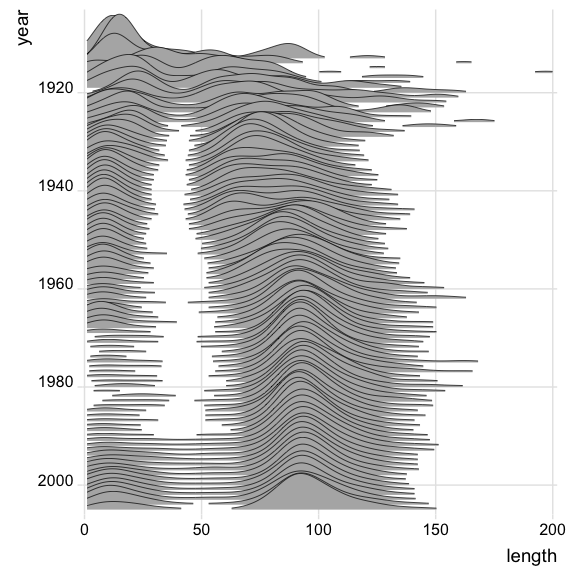
\includegraphics{./Images/ggridge.png}

Ce bookdown présent les éléments d'un cours de data science avec r. Il est reproductible, on peut en cloner les éléments à partir du \href{https://github.com/BenaventC/DataScienceBook}{repository}. Le texte est encore hasardeux mais les codes sont vérifiés. Il sera dynamique, modifié à mesure de nos cours, séminaires et ateliers.

L'illustration de couverture représente l'évolution de la longueur des films de la base \href{https://www.imdb.com/}{Imbd} et raconte en chiffres un aspect de l'histoire du cinéma. Jusqu'aux années 30, la longueur est hétérogène puis elle se se stabilise : les courts-métrages ont une durée de l'ordre de 15 mn qui se raccourcit avec les décennies, ce genre menace de disparaître dans les années 80 et reprend du poil de la bête dans les années 2000. Les films longs voient leur longueur s'accroître et se stabiliser autour d'un peu moins de 100 mn, soit une heure et quarante minutes. On observera enfin qu'au cours des années 1990 les films de taille intermédiaires réapparaissent. On devinera dans cette évolution l'émergence de standards, ou de conventions. Dans ce graphique il y a tous les éléments des data sciences contemporaines : un jeu de données riche et systématique, un modèle statistique fondamental avec la notion de densité de probabilité, une mesure, un critère de comparaison.

Les diagrammes ridges, c'est ainsi qu'on les appele, sont inspirés de la pochette de l'album \href{https://www.youtube.com/watch?v=7PtvIr2oiaE}{Unknown Pleasures de Joy division} sorti en pleine période New Wave, en 1979. Un article de Vice en rappele l'\href{https://i-d.vice.com/fr/article/pabjam/pourquoi-cette-pochette-dalbum-de-joy-division-a-inspire-le-monde-entier}{origine et le destin du graphisme} qu'on connait mieux imprimé sur des t-shirt que dans les cours de statistiques.

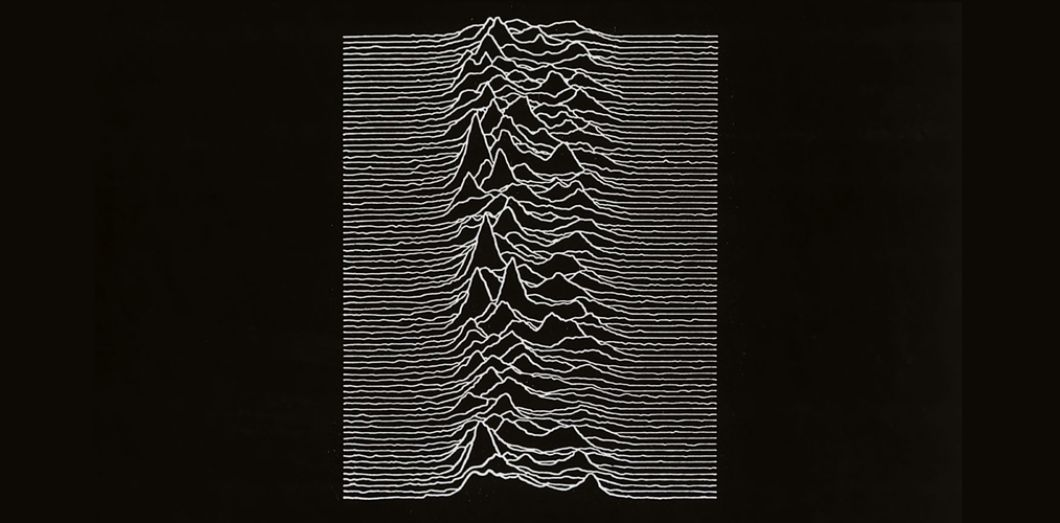
\includegraphics{./Images/joydivisiondetail.jpg}
\newpage

\hypertarget{plan-du-manuel}{%
\section{Plan du manuel}\label{plan-du-manuel}}

C'est un projet en cours, Le plan général projeté est le suivant. Certains chapitres sont publiés ( mêmes incomplets) d'autres sont dans les limbes. On les ajoutera progressivement.

\begin{itemize}
\tightlist
\item
  1 - L'environnement r x
\item
  2 - Installation et prise en main x
\item
  3 - Usage de ggplot - uni et bivarié x
\item
  4 - Usage de ggplot - multivarié x
\item
  5 - Tables avec flex
\item
  6 - Modèles factoriels (Psych) x
\item
  7 - AFC x
\item
  8 - MDS
\item
  9 - Clustering x
\item
  10 - Analyse de réseaux
\item
  11 - Analyse de variance et régression linéraire x
\item
  12 - Modèle linéaire généralisé x
\item
  13 - Modèles à décomposition d'erreur x
\item
  14 - Modèle d'équations structurelles (Lavaan)
\item
  15 - Times series
\item
  16 - Analyse spatiale et géographique
\item
  17 - Machine learning x
\end{itemize}

\hypertarget{les-jeux-de-donnuxe9es}{%
\section{Les jeux de données}\label{les-jeux-de-donnuxe9es}}

Au cours du développement, plusieurs cas pratiques - souvent réduit en volume pour rester exemplaire, seront employés. Les données sont partagées.

Voici la présentation des sets de données utilisées dans le syllabus. Ils sont disponibles dans le répertoire ``./data/''

\begin{itemize}
\tightlist
\item
  ESS : c'est une très belle base de données de sociologie
\item
  happydemics : observatoire de la présidentielle2022
\item
  NSPools
\item
  Arpur : commerce de paris
\item
  Botanic
\item
  \ldots{}
\end{itemize}

\hypertarget{le-cadre-technique-et-les-packages-utilisuxe9s}{%
\section{Le cadre technique et les packages utilisés}\label{le-cadre-technique-et-les-packages-utilisuxe9s}}

Ce \emph{syllabus} est écrit en \textbf{Markdown} \citep{allaire_rmarkdown_2021} et avec le package \textbf{Bookdown} \citep{R-bookdown}. Le code s'appuie sur \texttt{tidyverse} et emploie largement les ressources de \texttt{ggplot}. Les packages seront introduits au fur et à mesure mais un voici la liste complète.

\begin{Shaded}
\begin{Highlighting}[]
\FunctionTok{options}\NormalTok{(}\AttributeTok{tinytex.verbose =} \ConstantTok{TRUE}\NormalTok{)}
\NormalTok{knitr}\SpecialCharTok{::}\NormalTok{opts\_chunk}\SpecialCharTok{$}\FunctionTok{set}\NormalTok{(}\AttributeTok{echo =} \ConstantTok{TRUE}\NormalTok{, }\AttributeTok{include=}\ConstantTok{TRUE}\NormalTok{, }\AttributeTok{cache=}\ConstantTok{TRUE}\NormalTok{, }\AttributeTok{message=}\ConstantTok{FALSE}\NormalTok{, }\AttributeTok{warning=}\ConstantTok{FALSE}\NormalTok{)}

\CommentTok{\#boite à outils et dataviz}
\FunctionTok{library}\NormalTok{(tidyverse) }\CommentTok{\# inclut ggplot pour la viz, readr et }
\FunctionTok{library}\NormalTok{(cowplot) }\CommentTok{\#pour créer des graphiques composés}
\FunctionTok{library}\NormalTok{(ggridges) }\CommentTok{\# le joy division touch}
\FunctionTok{library}\NormalTok{(ggmosaic)}
\FunctionTok{library}\NormalTok{(ggcorrplot)}
\FunctionTok{library}\NormalTok{(corrplot) }\CommentTok{\#à supprimer}
\FunctionTok{library}\NormalTok{(ggthemes)}
\FunctionTok{library}\NormalTok{(colorspace) }\CommentTok{\#pour les couleurs}
\FunctionTok{library}\NormalTok{(wesanderson)}
\FunctionTok{library}\NormalTok{(RColorBrewer)}

\CommentTok{\#networks}
\FunctionTok{library}\NormalTok{(igraph)}
\FunctionTok{library}\NormalTok{(ggraph)}

\CommentTok{\# Accéder aux données}
\FunctionTok{library}\NormalTok{(rtweet)  }\CommentTok{\# une interface efficace pour interroger l\textquotesingle{}api de Twitter}

\CommentTok{\# NLP}
\FunctionTok{library}\NormalTok{(tokenizers)}
\FunctionTok{library}\NormalTok{(quanteda)}
\FunctionTok{library}\NormalTok{(quanteda.textstats)}
\FunctionTok{library}\NormalTok{(udpipe) }\CommentTok{\#annotation syntaxique}
\FunctionTok{library}\NormalTok{(tidytext)}
\FunctionTok{library}\NormalTok{(cleanNLP) }\CommentTok{\#annotation syntaxique}

\CommentTok{\#sentiment}
\FunctionTok{library}\NormalTok{(syuzhet)             }\CommentTok{\#analyse du sentimeent}

\CommentTok{\#mise en page des tableaux}
\FunctionTok{library}\NormalTok{(flextable)}

\CommentTok{\#statistiques et modèles}
\FunctionTok{library}\NormalTok{(lme4) }\CommentTok{\#pour des modèles plus complexe que les mco}
\FunctionTok{library}\NormalTok{(jtools) }\CommentTok{\#une série d\textquotesingle{}utiltaire pour bien représenter les résultats}
\FunctionTok{library}\NormalTok{(interactions) }\CommentTok{\#traitement des interactions}
\FunctionTok{library}\NormalTok{(nlme)}\CommentTok{\#pour les hlm}
\FunctionTok{library}\NormalTok{(psych) }\CommentTok{\#pour la psychometrie}

\CommentTok{\#ACP et AFCM}
\FunctionTok{library}\NormalTok{(}\StringTok{"FactoMineR"}\NormalTok{)}
\FunctionTok{library}\NormalTok{(}\StringTok{"factoextra"}\NormalTok{)}

\CommentTok{\#ML}
\FunctionTok{library}\NormalTok{(caret)}

\CommentTok{\#regression}
\FunctionTok{library}\NormalTok{(lme4)}
\FunctionTok{library}\NormalTok{(jtools)}
\FunctionTok{library}\NormalTok{(interactions)}
\FunctionTok{library}\NormalTok{(betareg)}
\FunctionTok{library}\NormalTok{(lavaan)}

\CommentTok{\# Utilitaires}
\FunctionTok{library}\NormalTok{(citr) }\CommentTok{\#pour insérer des références dans le markdown}

\FunctionTok{library}\NormalTok{(MASS)}


\CommentTok{\#config plot}
\FunctionTok{theme\_set}\NormalTok{(}\FunctionTok{theme\_minimal}\NormalTok{())}
\end{Highlighting}
\end{Shaded}

L'ensemble du code est disponible \href{https://github.com/BenaventC/Datasciences}{sur github}. A ce stade c'est encore embryonnaire. Les proches et nos étudiants pourrons cependant y voir l'évolution du projet et de la \href{https://benaventc.github.io/Datascience/}{progression}. Une version pdf est disponible ici.

Quelques conventions d'écriture du code r

\begin{itemize}
\tightlist
\item
  On dénomme les data frames de manière générale \texttt{df}, les tableaux intermédiaires sont appelé systématiquement \texttt{foo}
\item
  Gestion des palettes de couleurs
  ** une couleur :'' royalblue''
  ** deux couleurs
  ** 3 à 7 couleurs
\item
  On emploie autant que possible le dialecte tidy.
\item
  Les chunks sont notés en 4 chiffres : 2 pour le chapitre et deux pour le chunck. 0502 est le second chunk du chapitre 5.
\item
  On commente au maximum les lignes de code pour épargner le corps du texte et le rendre lisible
\end{itemize}

\hypertarget{intro}{%
\chapter{Introduction aux data sciences}\label{intro}}

L'objet du manuel est de donner un aperçu général des méthodes d'analyses de données et de data sciences Mais avant de s'engager dans les procédures une réflexion épistémologique et historique peut être utile. Si les méthodes sont puissantes, inventives, ils faut aussi s'interroger sur leur conditions d'émergences.
La discipline fût la statistique, elle alimenta milles champs spécifiques : économétrie, psychométrie, biostatistiques. Derrières les problèmes l'avance des mathématiques pour caractériser les modèles proposés. Elle s'est laissée aller à d'autres terminologies : analyse des données, data mining, Machien learning, deep learning.

\hypertarget{science-art-technique-et-pratiques}{%
\section{Science, art, technique et pratiques}\label{science-art-technique-et-pratiques}}

Plutôt que le terme consacré de data sciences, il vaudrait mieux parler de data ingénierie dans la mesure où le data scientiste participe à un processus de production qui va de l'acquisition des données à leur propagation dans l'organisation ou la société. La technique domine sur la science et l'unité se trouve dans l'intégration de ce processus. La révolution des données vient de l'interopérabilité croissante de ces techniques et d'une intégration qui fluidifie le passage d'une étape à une autre. Standards et langages en sont les éléments clés.

Du côté des sciences, ce dont bénéficie l'univers des data sciences, c'est l'héritage de cultures statistiques foisonnantes qui après s'être développées dans leur cocon disciplinaire, se retrouvent désormais rassemblées dans un même langage. Bien sur il y a de manière sous-jascente les mathématiques et les statistiques qui construisent les fondements des modèles et des techniques.

Mais leur développement s'est fait souvent quand le scientifique se retrouve face à un problème où une observation. Prenons le cas des psychologues qui ont inventé l'analyse factorielle dans le but de pouvoir tester certains de leurs concepts : un degré d'intelligence, une personnalité, des attitudes.

Ou celui des écologues qui souhaitent estimer une population de poisson dans une rivière, problème qui a donné naissance aux modèles de capture/recapture. On pourrait ajouter les géographes avec les modèles d'analyse spatiale, les financiers face à la variabilité des cours des places boursières, etc. Celui des économètres est peut-être le plus évident. Les biostatisticiens sont des contributeurs importants.

Ce que la technique apporte c'est l'intégration par un langage et donc un ensemble de conventions, incarnées par r et python, algorithmes, et de programmes qui ne sont plus spécifiques à un domaine, mais peuvent circuler de l'un à l'autre. C'est ainsi que le catalogues de toutes les techniques psychométriques devient accessible aux autres disciplines par le biais d'un package en particulier, psych. De la même manière l'outillage des linguiste devient accessible aux autres disciplines, pensons aux économiste qui intégrent dans le indicateurs des sources textuelle telle que l'analyse du sentiment. ( ref)

L'interopérabilité apportée par ces langages ne se définit pas que par l'algorithme qui aurait été porté d'un autre langage vers celui-ci (des cas de réécriture ?) mais aussi par des programme passerelle qui à partir de r permettent d'activité des algorithme écrit en C, en javascript ou tout autre langage ``plus informatique'' et souvent plus efficace.

\hypertarget{une-courte-histoires-des-logiciels-statistiques}{%
\section{Une courte histoires des logiciels statistiques}\label{une-courte-histoires-des-logiciels-statistiques}}

Ce qu'on observe dans l'évolution des logiciels

\begin{itemize}
\tightlist
\item
  1980 : stat-itcf
\item
  1980 : SAS comme accès à r
\item
  1990 : SPSS
\item
  stata
\item
  1997 : s dès 976 puis r, 1996 fre sofsware as r. le CRAN nait en 1997. 2003 création dez r foundation.
\item
  1991 - 2001: Python - Guido van Rossum - Python Software Foundation, créée en 2001
\item
  keras
\item
  tensor flow
\end{itemize}

\url{http://www.deenov.com/blog-deenov/histoire-du-logiciel-spad.aspx}

Un des grand mouvement du domaine est l'hésitation entre le programmatique et le no-code. La pression commerciale conduit certains acteurs à encourager l'usage de sur-couche logiciel qui débarrasse l'utilisateur de l'exigence techniques, il peut se laisser guider par l'intuition, mais l'aliène en dissimulant la mécanique profonde des processus de traitement des données.

Le succès de python et de r réside dans

\begin{itemize}
\tightlist
\item
  La modularisation : langage de base /fonction/ package et notion de dépendance
\item
  L'interopérabilité pas toujours parfaite ( versions, classes de données)
\item
  La cumulativité : les fonction s'ajoutent aux fonctions, se sédimentent
\item
  L'accès
\end{itemize}

\hypertarget{le-processus-de-traitement-des-donnuxe9es}{%
\section{Le processus de traitement des données}\label{le-processus-de-traitement-des-donnuxe9es}}

Les data sciences ne sont finalement que l'intégration d'un flot de traitement des données qui va de l'acquisition à la divulgation.

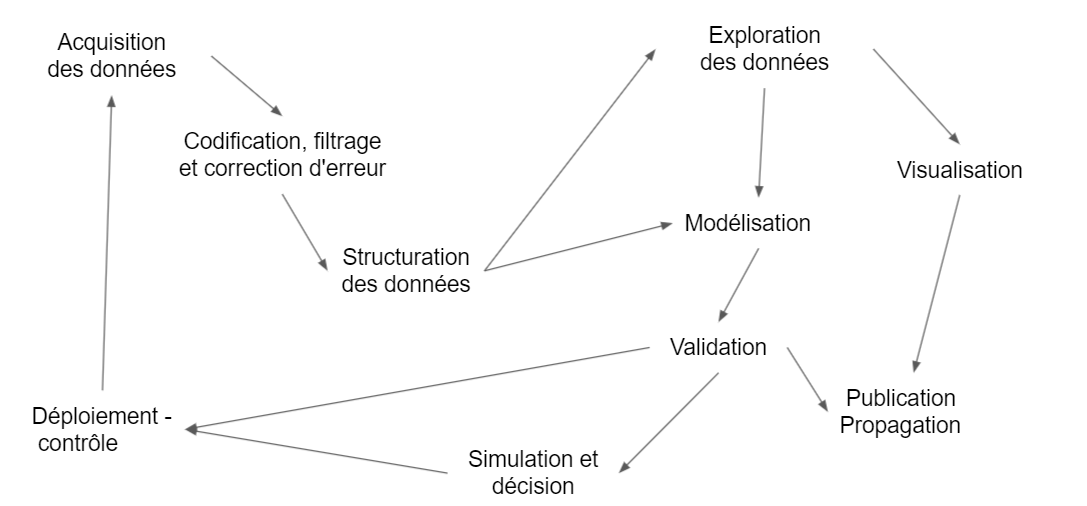
\includegraphics{./Images/datascience2.png}

\begin{itemize}
\tightlist
\item
  Acquisition
\item
  Codification , filtrage et correction d'erreur
\item
  Structuration des données : api, open data
\item
  Exploration
\item
  Modélisation :
\item
  validation : tests versus AB testing
\item
  Simulation et décision
\item
  Vizualisation et sensemaking
\item
  Déploiement :
\item
  Contrôle :
\item
  Publication : dash board, pdf , slide etc, webb site
\end{itemize}

\hypertarget{les-facteurs-sociaux-du-duxe9veloppement-des-datasciences}{%
\section{Les facteurs sociaux du développement des datasciences}\label{les-facteurs-sociaux-du-duxe9veloppement-des-datasciences}}

Ces développements sont favorisés par un environnement fertile dont quatre facteurs se renforcent mutuellement. La constitution d'un système de communication commun organisé autour de peu de langage, et d'un ensemble de normes de données mais aussi la vitalité d'une communauté. La multiplicité des sources de données et l'évolution des technologies de la mesure et du nombre constitue un second groupe de facteurs.

\hypertarget{une-lingua-franca}{%
\subsection{Une lingua franca}\label{une-lingua-franca}}

La lingua franca est la langue des ports et du commerce de la méditerranée au XIVème siècle, un mélange de langage qui sert l'échange, un commun pourrait-on dire aujourd'hui. C'est ce que sont devenus python et r parmi d'autres, la seconde langue après l'anglais qui s'est imposé comme la langue d'écriture. Le langage des scientifiques est sans doute désormais un pidgin, un créole d'anglais, et de r ou de python, sans compter les sparc, les C+++ ou javascript. Les langues de la donnée se mêlent volontiers, elle sont de plus en plus agnostique.

L'environnement r par exemple devient de plus en plus ouverts à python, à la fois de manière directe en permettant de coder dans un même document des calculs en r pluis en python, mais aussi de manière indirecte parce que prolifèrent des packages passerelles permettant d'aller chercher des ressources écrites dans un autre langage.

\hypertarget{une-communautuxe9}{%
\subsection{Une communauté}\label{une-communautuxe9}}

Le second facteur, intimement lié au premier, est la constitution d'une large communauté de développeurs et utilisateurs qui se retrouvent aujourd'hui dans des plateformes de dépôts (Github, Gitlab), de plateformes de type quora (StalkOverFlow), de tutoriaux, de blogs (BloggeR), de journaux (Journal of Statistical Software) et de bookdown. Des ressources abondantes sont disponibles et facilitent la formation des chercheurs et des data scientists. Toutes les conditions sont réunies pour engendrer une effervescence créative.

Cette communauté se reproduit à petite échelles dans les procédures de laboratoire et les conventions de travail en commun des chercheurs. Elle peut se développer autant verticalement qu'horizontalement : des hubs qui concentrent l'ensemble des acteurs et des ressources, qu'un grand nombre de micro communauté focalisés sur des problèmes très locaux.

\hypertarget{la-multiplication-des-sources-de-donnuxe9es.}{%
\subsection{La multiplication des sources de données.}\label{la-multiplication-des-sources-de-donnuxe9es.}}

Le troisième est la multiplication des sources de données et leur facilité d'accès. Les données privées, et en particulier celles des réseaux sociaux, même si un péage doit être payé pour accéder aux APIs, popularisent le traitement de données massives.

Le mouvement des données ouvertes (open data) proposent et facilitent accès à des milliers de corps de données : retards de la SNCF, grand débat, le formidable travail de l'Insee, european survey etc.

\hypertarget{de-la-statistique-uxe0-lia}{%
\subsection{de la statistique à l'IA}\label{de-la-statistique-uxe0-lia}}

Le retour au boites noires dans les années 2000. Ce qui distingue les statistiques traditionnelles de l'approche machine learning réside d'abord par une approche de la modélisation différente.

Les modèles statistiques et économétriques considèrent une structure de relation, la spécification du modèle (ex : le modèle linéaire), mais aussi des modèles de distribution des erreurs qui définissent le cadre d'estimation. L'évaluation passe par le test des hypothèses sur les paramètres et par la qualité d'ajustement.

Le machine learning, se concentre sur la valeur prédictive, et considère n'importe quelle spécification même si elle est peu intelligible et comprend de grandes quantités de paramètres sur lesquels aucun test n'est produit.

Les deux approches ont plutôt tendance à ce compléter, les première testant des théories, les secondes procurant aux première de nouvelles hypothèse par de nouvelle mesure. Pour en donner un exemple simple, l'analyse de sentiment emploie des modèles complexes pour le prédire avec le seul texte, l'IA permet d'enrichir des données empiriques par exemple en testant en finance la relation de cet indicateurs aux prix de marché. Un autre exemple en marketing.

Les méthodes disponibles se sont accumulées depuis ces dernières 20 années. faisons-en une courte liste.

\begin{itemize}
\tightlist
\item
  1956 :perceptron
\item
  1963 : arbre de décision
\item
  2005 : CNN
\item
  2008 : lda topic
\item
  2013 : word2vec
\item
  2018 : transformers
\item
  \ldots.
\end{itemize}

KNN, SVM, rf et le retour des réseaux de neurones.

\hypertarget{conclusion}{%
\section{Conclusion}\label{conclusion}}

Il ne reste plus qu'à soulever le capot et de mettre les mains dans le cambouis.

Et à se rappeler que si la nécessité de se faire remarquer à conduit les acteurs du domaine à envisager des data sciences, que c'est d'abord un art d'écriture, et une pratique qui permet à leurs artisans de s'échanger des secrets de fabrique.

On remerciera tous ceux qui développent des Packages, nous aurons le point de vue de ceux qui les utilisent. Ce cours est aussi un livre de recette, celui d'un chercheur en sciences sociales qui picore dans l'immensité de la production pour trouver des procédures reproductibles par ses étudiants.

\hypertarget{prise-en-main-de-r}{%
\chapter{Prise en main de r}\label{prise-en-main-de-r}}

Pour démarrer :

\begin{itemize}
\tightlist
\item
  1 - Télécharger et installer r sur le site du Comprehensive r Archive Network
\item
  2 - Télécharger et installer Rstudio.(version free)
\item
  3 - Dans le cadre de cet atelier, on adopte la méthode du \href{https://rmarkdown.rstudio.com/lesson-1.html}{rmarkdown}. On recommande fortement de lire l'ouvrage de référence, même si la prise en main est très rapide.
\item
  4 - Il est désormais indispensable d'utiliser le package \texttt{tidyverse} et en particulier les fonctions de manipulation et de pipe (\%\textgreater\%) fournies par \texttt{dplyr}. Ce sera donc le premier package à installer (attention, il appele de nombreuses dépendences, l'installation peut prendre plusieurs minutes )
\end{itemize}

\hypertarget{la-convention-du-rmarkdown}{%
\section{La convention du Rmarkdown}\label{la-convention-du-rmarkdown}}

Différentes manières d'interagir avec r sont possibles : la première est le mode console, pour de petite opérations et un utilisateur chevronné, celà peut être commode car rapide mais très rapidement on sera amené à enregistrer les opérations dans des scripts. Une idée novatrice a été d'intégrer l'ensemble des élements dans un seul document : le script découpé en petits éléments : des chunks, le commentaire et l'analyse verbabe dans un format texte, et le résultat. Dans l'univers python il s'agit des carnets Jupiter, pour r c'est le rmarkdown.

C'est un dialecte du markdown générique adapté au langage r. On recommande au lecteur d'en lire \href{https://bookdown.org/yihui/rmarkdown/}{le manuel} et de le garder dans ses onglets.

Quelques éléments de base :

un document markdown est composé de plusieurs éléments

\begin{enumerate}
\def\labelenumi{\arabic{enumi}.}
\tightlist
\item
  Yalm : dans cet entête les éléments essentiels sont définis et paramétrés
\item
  Texte : il suit les conventions de mise en forme du html :

  \begin{itemize}
  \tightlist
  \item
    des \# pour les niveau de titres
  \item
    une syntaxe (x){[}.xxx{]} pour des liens vers les URLS ou des images.
  \end{itemize}
\item
  Les chunks sont isolés par 3 tiks au début et à la fin.
\item
  Résultats apparaissent sous les chunks après avoir été exécutés
\end{enumerate}

Ce document peut être publié sous différents formats : html, pdf ou même word.

Il comprend les éléments suivants :

\begin{itemize}
\tightlist
\item
  Plan
\item
  Texte
\item
  Code
\item
  Résultats
\item
  Bibliographie
\item
  Références
\item
  Liens
\item
  Images
\end{itemize}

\hypertarget{lire-les-donnuxe9es}{%
\section{Lire les données}\label{lire-les-donnuxe9es}}

La première étape c'est la lecture des données. On commence par lecture de fichiers locaux, dont les formats sont multiples : csv, tsv, xlsx, Spss, etc\ldots{} Pour chacun d'eux existe une fonction dédiée.
Le package \texttt{readr} contribue à cette tâche pour les fichiers *.csv.

\begin{Shaded}
\begin{Highlighting}[]
\NormalTok{df }\OtherTok{\textless{}{-}} \FunctionTok{read\_csv}\NormalTok{(}\StringTok{"./Data/BXL\_listings.csv"}\NormalTok{)}
\FunctionTok{head}\NormalTok{(df,}\DecValTok{5}\NormalTok{)}
\end{Highlighting}
\end{Shaded}

\begin{verbatim}
## # A tibble: 5 x 16
##      id name       host_id host_~1 neigh~2 neigh~3 latit~4 longi~5 room_~6 price
##   <dbl> <chr>        <dbl> <chr>   <lgl>   <chr>     <dbl>   <dbl> <chr>   <dbl>
## 1  2352 Triplex-2~    2582 Oda     NA      Molenb~    50.9    4.31 Entire~    91
## 2  2354 COURT/Lon~    2582 Oda     NA      Molenb~    50.9    4.31 Entire~    74
## 3 45145 B&B Welco~  199370 <NA>    NA      Bruxel~    50.9    4.37 Hotel ~   120
## 4 48180 Top Apart~  219560 Ahmet   NA      Woluwe~    50.8    4.41 Entire~   200
## 5 52796 Bright ap~  244722 Pierre  NA      Ixelles    50.8    4.36 Entire~    74
## # ... with 6 more variables: minimum_nights <dbl>, number_of_reviews <dbl>,
## #   last_review <date>, reviews_per_month <dbl>,
## #   calculated_host_listings_count <dbl>, availability_365 <dbl>, and
## #   abbreviated variable names 1: host_name, 2: neighbourhood_group,
## #   3: neighbourhood, 4: latitude, 5: longitude, 6: room_type
\end{verbatim}

Il est possible aussi d'accéder en direct aux données du web, c'est bien utile pour s'assurer que les données sont bien fraîches. Par exemple une connexion à \href{https://github.com/nsppolls/nsppolls}{Nsppolls} qui propose une compilation de tous les sondages d'intention de vote de la présidentielle 2022.

\begin{Shaded}
\begin{Highlighting}[]
\NormalTok{df\_pol }\OtherTok{\textless{}{-}} \FunctionTok{read\_delim}\NormalTok{(}\StringTok{"https://raw.githubusercontent.com/nsppolls/nsppolls/master/presidentielle.csv"}\NormalTok{, }
                     \AttributeTok{delim =} \StringTok{","}\NormalTok{, }\AttributeTok{escape\_double =} \ConstantTok{FALSE}\NormalTok{, }\AttributeTok{trim\_ws =} \ConstantTok{TRUE}\NormalTok{)}
\end{Highlighting}
\end{Shaded}

Bien d'autre possibilités sont offertes, on pourra utiliser des API, des programmes de scrapping., ire en bouche des fichiers dans un répertoire, interroger des bases SQL des \href{https://sql.sh/sgbd}{SGBD}) ou d'autres systèmes.

\hypertarget{la-diversituxe9-des-formats}{%
\subsection{La diversité des formats}\label{la-diversituxe9-des-formats}}

Peu de formats échappent à r, ils peuvent faire appel à des packages spécifiques

\begin{itemize}
\tightlist
\item
  excell
\item
  Json
\item
  shape et autre données géographiques.
\item
  les formats bibliographiques sont plus exotique : bib et ris
\item
  les xml pourront donner des maux de têtes.
\end{itemize}

\hypertarget{dplyr-pour-manipuler-les-donnuxe9es}{%
\section{\texorpdfstring{\texttt{Dplyr} pour manipuler les données}{Dplyr pour manipuler les données}}\label{dplyr-pour-manipuler-les-donnuxe9es}}

Dès lors que les données sont chargées en mémoire il va souvent être nécessaire d'en travailler, l'aspect et la structure. L'aspect concerne les formats et les significations, les recodages. La structure est relative à la forme des tableaux. Il faudra souvent traiter les données brutes pour proposer à nos modèles des structures appropriées.

\texttt{Dplyr} est un des packages essentiels de la suite tidyverse. Il permet de manipuler aisément les données et mérite une étude approfondie. Un \href{https://dplyr.tidyverse.org/articles/dplyr.html}{point de départ} ou en français : \href{http://larmarange.github.io/analyse-R/manipuler-les-donnees-avec-dplyr.html}{dplyr}.

Deux idées sont au coeur de \texttt{Dplyr} d'abord celle du pipe, ensuite celle du verbe. \texttt{Dplyr} encourage une approche processus et performative.

\hypertarget{des-pipes}{%
\subsection{Des pipes \%\textgreater\%}\label{des-pipes}}

Une grand part de l'intérêt de dplyr est de reprendre un opérateur de magritr très utile : le pipe noté \texttt{data\ \%\textgreater{}\%\ f()\ \%\textgreater{}\%\ g()..}. Celui ci permet de passer le résultat de l'opération à gauche f() sur les données \texttt{data}, dans la fonction g() à droite.

Un exemple simple : dans la ligne de code suivante, une première fonction lit le fichier CSV, et envoie le résultat de cette lecture dans une fonction graphique élémentaire: compter les occurrences des modalités de la variable room\_type.

\begin{Shaded}
\begin{Highlighting}[]
\NormalTok{g }\OtherTok{\textless{}{-}} \FunctionTok{read\_csv}\NormalTok{(}\StringTok{"./Data/BXL\_listings.csv"}\NormalTok{) }\SpecialCharTok{\%\textgreater{}\%} 
  \FunctionTok{ggplot}\NormalTok{(}\FunctionTok{aes}\NormalTok{(}\AttributeTok{x=}\NormalTok{room\_type))}\SpecialCharTok{+}
  \FunctionTok{geom\_bar}\NormalTok{()}\SpecialCharTok{+}
  \FunctionTok{coord\_flip}\NormalTok{()}\SpecialCharTok{+}
  \FunctionTok{labs}\NormalTok{(}\AttributeTok{x=}\ConstantTok{NULL}\NormalTok{, }\AttributeTok{y=} \StringTok{"Fréquence"}\NormalTok{, }\AttributeTok{title=}\StringTok{" Distribution des types de logement à Bruxelles en 2020"}\NormalTok{)}
\NormalTok{g}
\end{Highlighting}
\end{Shaded}

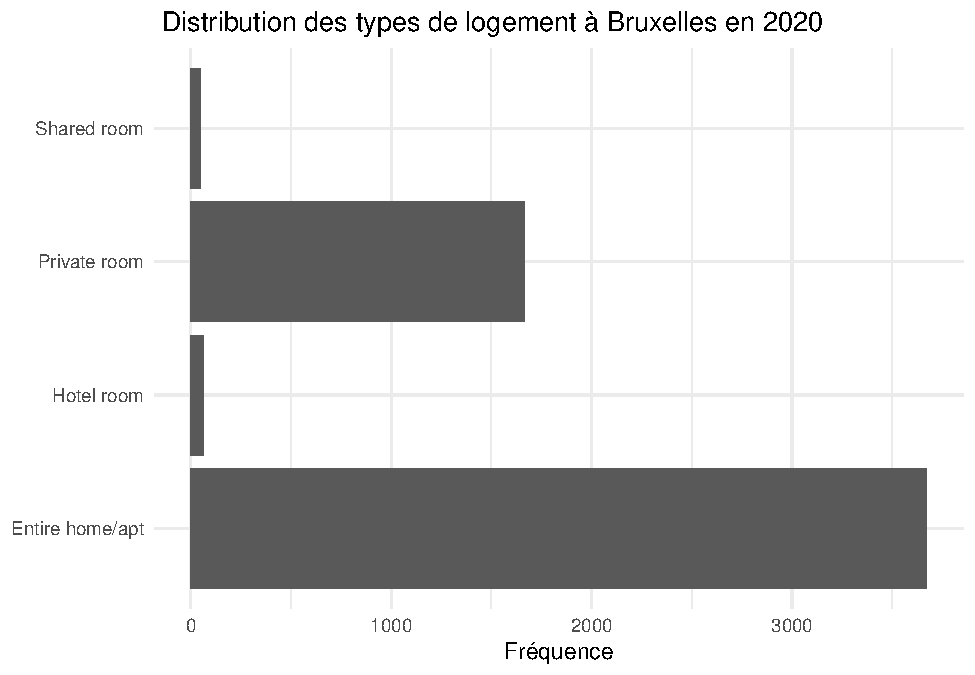
\includegraphics{bookdown-demo_files/figure-latex/0203-1.pdf}

\hypertarget{des-verbes}{%
\subsection{Des verbes}\label{des-verbes}}

L'originalité de \texttt{dplyr}est de définir les fonctions comme des verbes. Chaque verbe désigne une action particulière. On va les examiner progressivement.
* transformer une variable,
* filtrer les observations selon un critère,
* isoler des variables,
* les grouper pour en calculer des résultats statistiques (somme, moyenne, variance, max min etc),
* les déployer selon un format long ou les distribuer en différents critères,
* les fusionner enfin.

\hypertarget{mutate}{%
\subsubsection{Mutate}\label{mutate}}

En Français c'est ``transformer''. On modifie la valeur d'une variable par une fonction plus ou moins complexe, éventuellement en ajoutant des conditions.

Dans notre exemple, faisant au plus simple, puisque la distribution est asymétrique, une transformation du prix par les log10 peut donner des résultats intéressants. Et c'est le cas, on retrouve une distribution qui semble être gaussienne.

\begin{Shaded}
\begin{Highlighting}[]
\NormalTok{g }\OtherTok{\textless{}{-}} \FunctionTok{read\_csv}\NormalTok{(}\StringTok{"./Data/BXL\_listings.csv"}\NormalTok{) }\SpecialCharTok{\%\textgreater{}\%} 
  \FunctionTok{mutate}\NormalTok{(}\AttributeTok{price=}\FunctionTok{log10}\NormalTok{(price))}\SpecialCharTok{\%\textgreater{}\%}
  \FunctionTok{ggplot}\NormalTok{(}\FunctionTok{aes}\NormalTok{(}\AttributeTok{x=}\NormalTok{price))}\SpecialCharTok{+}
  \FunctionTok{geom\_histogram}\NormalTok{()}
\NormalTok{g}
\end{Highlighting}
\end{Shaded}

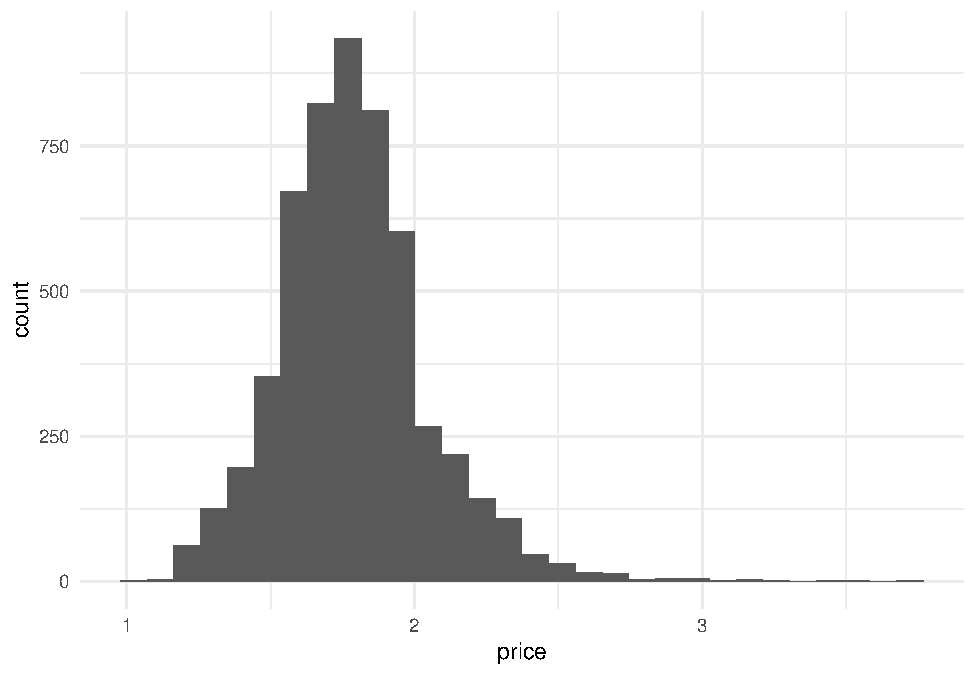
\includegraphics{bookdown-demo_files/figure-latex/0204-1.pdf}

\hypertarget{filter}{%
\subsubsection{Filter}\label{filter}}

On peut vouloir se concentrer sur une sous population. Par exemple les chambres privées.

\begin{Shaded}
\begin{Highlighting}[]
\NormalTok{g }\OtherTok{\textless{}{-}} \FunctionTok{read\_csv}\NormalTok{(}\StringTok{"./Data/BXL\_listings.csv"}\NormalTok{) }\SpecialCharTok{\%\textgreater{}\%} 
  \FunctionTok{filter}\NormalTok{(room\_type}\SpecialCharTok{==}\StringTok{"Private room"}\NormalTok{ ) }\SpecialCharTok{\%\textgreater{}\%} 
    \FunctionTok{mutate}\NormalTok{(}\AttributeTok{price=}\NormalTok{price)}\SpecialCharTok{\%\textgreater{}\%}
  \FunctionTok{ggplot}\NormalTok{(}\FunctionTok{aes}\NormalTok{(}\AttributeTok{x=}\FunctionTok{log10}\NormalTok{(price)))}\SpecialCharTok{+}
  \FunctionTok{geom\_histogram}\NormalTok{()}
\NormalTok{g}
\end{Highlighting}
\end{Shaded}

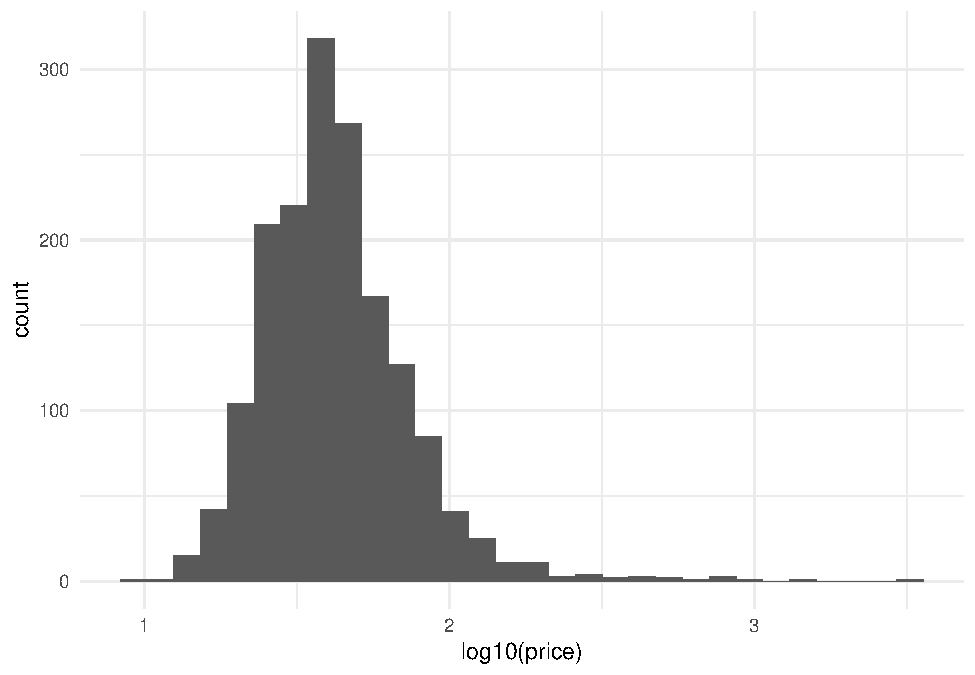
\includegraphics{bookdown-demo_files/figure-latex/0205-1.pdf}

\hypertarget{select}{%
\subsubsection{select}\label{select}}

On peut sélectionner des colonnes pour créer un tableau spécifique. On en profite pour introduire `\href{https://ardata-fr.github.io/flextable-book/index.html}{flextable}' , une solution élégante pour éditer des tableaux en html.

\begin{Shaded}
\begin{Highlighting}[]
\NormalTok{foo }\OtherTok{\textless{}{-}} \FunctionTok{read\_csv}\NormalTok{(}\StringTok{"./Data/BXL\_listings.csv"}\NormalTok{) }\SpecialCharTok{\%\textgreater{}\%}
\NormalTok{  dplyr}\SpecialCharTok{::}\FunctionTok{select}\NormalTok{(room\_type,price) }

\NormalTok{ft }\OtherTok{\textless{}{-}} \FunctionTok{flextable}\NormalTok{(foo[ }\FunctionTok{sample.int}\NormalTok{(}\DecValTok{10}\NormalTok{),])}\SpecialCharTok{\%\textgreater{}\%}
   \FunctionTok{set\_header\_labels}\NormalTok{(}\AttributeTok{room\_type=}\StringTok{"Type de logement"}\NormalTok{,}
  \AttributeTok{price =} \StringTok{"Prix en euros"}\NormalTok{)}\SpecialCharTok{\%\textgreater{}\%}
  \FunctionTok{theme\_vanilla}\NormalTok{()}\SpecialCharTok{\%\textgreater{}\%} \FunctionTok{fontsize}\NormalTok{(}\AttributeTok{size =} \DecValTok{9}\NormalTok{)}\SpecialCharTok{\%\textgreater{}\%}
  \FunctionTok{autofit}\NormalTok{()}
\NormalTok{ft}
\end{Highlighting}
\end{Shaded}

\providecommand{\docline}[3]{\noalign{\global\setlength{\arrayrulewidth}{#1}}\arrayrulecolor[HTML]{#2}\cline{#3}}

\setlength{\tabcolsep}{2pt}

\renewcommand*{\arraystretch}{1.5}

\begin{longtable}[c]{|p{1.58in}|p{1.25in}}



\hhline{>{\arrayrulecolor[HTML]{666666}\global\arrayrulewidth=2pt}->{\arrayrulecolor[HTML]{666666}\global\arrayrulewidth=2pt}-}

\multicolumn{1}{!{\color[HTML]{000000}\vrule width 0pt}>{\raggedright}p{\dimexpr 1.58in+0\tabcolsep+0\arrayrulewidth}}{\fontsize{11}{11}\selectfont{\textcolor[HTML]{000000}{\global\setmainfont{Arial}{\textbf{Type\ de\ logement}}}}} & \multicolumn{1}{!{\color[HTML]{000000}\vrule width 0pt}>{\raggedleft}p{\dimexpr 1.25in+0\tabcolsep+0\arrayrulewidth}!{\color[HTML]{000000}\vrule width 0pt}}{\fontsize{11}{11}\selectfont{\textcolor[HTML]{000000}{\global\setmainfont{Arial}{\textbf{Prix\ en\ euros}}}}} \\

\noalign{\global\setlength{\arrayrulewidth}{2pt}}\arrayrulecolor[HTML]{666666}\cline{1-2}

\endfirsthead

\hhline{>{\arrayrulecolor[HTML]{666666}\global\arrayrulewidth=2pt}->{\arrayrulecolor[HTML]{666666}\global\arrayrulewidth=2pt}-}

\multicolumn{1}{!{\color[HTML]{000000}\vrule width 0pt}>{\raggedright}p{\dimexpr 1.58in+0\tabcolsep+0\arrayrulewidth}}{\fontsize{11}{11}\selectfont{\textcolor[HTML]{000000}{\global\setmainfont{Arial}{\textbf{Type\ de\ logement}}}}} & \multicolumn{1}{!{\color[HTML]{000000}\vrule width 0pt}>{\raggedleft}p{\dimexpr 1.25in+0\tabcolsep+0\arrayrulewidth}!{\color[HTML]{000000}\vrule width 0pt}}{\fontsize{11}{11}\selectfont{\textcolor[HTML]{000000}{\global\setmainfont{Arial}{\textbf{Prix\ en\ euros}}}}} \\

\noalign{\global\setlength{\arrayrulewidth}{2pt}}\arrayrulecolor[HTML]{666666}\cline{1-2}\endhead



\multicolumn{1}{!{\color[HTML]{000000}\vrule width 0pt}>{\raggedright}p{\dimexpr 1.58in+0\tabcolsep+0\arrayrulewidth}}{\fontsize{9}{9}\selectfont{\textcolor[HTML]{000000}{\global\setmainfont{Arial}{Entire\ home/apt}}}} & \multicolumn{1}{!{\color[HTML]{000000}\vrule width 0pt}>{\raggedleft}p{\dimexpr 1.25in+0\tabcolsep+0\arrayrulewidth}!{\color[HTML]{000000}\vrule width 0pt}}{\fontsize{9}{9}\selectfont{\textcolor[HTML]{000000}{\global\setmainfont{Arial}{65}}}} \\

\noalign{\global\setlength{\arrayrulewidth}{0.5pt}}\arrayrulecolor[HTML]{666666}\cline{1-2}



\multicolumn{1}{!{\color[HTML]{000000}\vrule width 0pt}>{\raggedright}p{\dimexpr 1.58in+0\tabcolsep+0\arrayrulewidth}}{\fontsize{9}{9}\selectfont{\textcolor[HTML]{000000}{\global\setmainfont{Arial}{Entire\ home/apt}}}} & \multicolumn{1}{!{\color[HTML]{000000}\vrule width 0pt}>{\raggedleft}p{\dimexpr 1.25in+0\tabcolsep+0\arrayrulewidth}!{\color[HTML]{000000}\vrule width 0pt}}{\fontsize{9}{9}\selectfont{\textcolor[HTML]{000000}{\global\setmainfont{Arial}{85}}}} \\

\noalign{\global\setlength{\arrayrulewidth}{0.5pt}}\arrayrulecolor[HTML]{666666}\cline{1-2}



\multicolumn{1}{!{\color[HTML]{000000}\vrule width 0pt}>{\raggedright}p{\dimexpr 1.58in+0\tabcolsep+0\arrayrulewidth}}{\fontsize{9}{9}\selectfont{\textcolor[HTML]{000000}{\global\setmainfont{Arial}{Entire\ home/apt}}}} & \multicolumn{1}{!{\color[HTML]{000000}\vrule width 0pt}>{\raggedleft}p{\dimexpr 1.25in+0\tabcolsep+0\arrayrulewidth}!{\color[HTML]{000000}\vrule width 0pt}}{\fontsize{9}{9}\selectfont{\textcolor[HTML]{000000}{\global\setmainfont{Arial}{74}}}} \\

\noalign{\global\setlength{\arrayrulewidth}{0.5pt}}\arrayrulecolor[HTML]{666666}\cline{1-2}



\multicolumn{1}{!{\color[HTML]{000000}\vrule width 0pt}>{\raggedright}p{\dimexpr 1.58in+0\tabcolsep+0\arrayrulewidth}}{\fontsize{9}{9}\selectfont{\textcolor[HTML]{000000}{\global\setmainfont{Arial}{Entire\ home/apt}}}} & \multicolumn{1}{!{\color[HTML]{000000}\vrule width 0pt}>{\raggedleft}p{\dimexpr 1.25in+0\tabcolsep+0\arrayrulewidth}!{\color[HTML]{000000}\vrule width 0pt}}{\fontsize{9}{9}\selectfont{\textcolor[HTML]{000000}{\global\setmainfont{Arial}{80}}}} \\

\noalign{\global\setlength{\arrayrulewidth}{0.5pt}}\arrayrulecolor[HTML]{666666}\cline{1-2}



\multicolumn{1}{!{\color[HTML]{000000}\vrule width 0pt}>{\raggedright}p{\dimexpr 1.58in+0\tabcolsep+0\arrayrulewidth}}{\fontsize{9}{9}\selectfont{\textcolor[HTML]{000000}{\global\setmainfont{Arial}{Hotel\ room}}}} & \multicolumn{1}{!{\color[HTML]{000000}\vrule width 0pt}>{\raggedleft}p{\dimexpr 1.25in+0\tabcolsep+0\arrayrulewidth}!{\color[HTML]{000000}\vrule width 0pt}}{\fontsize{9}{9}\selectfont{\textcolor[HTML]{000000}{\global\setmainfont{Arial}{120}}}} \\

\noalign{\global\setlength{\arrayrulewidth}{0.5pt}}\arrayrulecolor[HTML]{666666}\cline{1-2}



\multicolumn{1}{!{\color[HTML]{000000}\vrule width 0pt}>{\raggedright}p{\dimexpr 1.58in+0\tabcolsep+0\arrayrulewidth}}{\fontsize{9}{9}\selectfont{\textcolor[HTML]{000000}{\global\setmainfont{Arial}{Entire\ home/apt}}}} & \multicolumn{1}{!{\color[HTML]{000000}\vrule width 0pt}>{\raggedleft}p{\dimexpr 1.25in+0\tabcolsep+0\arrayrulewidth}!{\color[HTML]{000000}\vrule width 0pt}}{\fontsize{9}{9}\selectfont{\textcolor[HTML]{000000}{\global\setmainfont{Arial}{80}}}} \\

\noalign{\global\setlength{\arrayrulewidth}{0.5pt}}\arrayrulecolor[HTML]{666666}\cline{1-2}



\multicolumn{1}{!{\color[HTML]{000000}\vrule width 0pt}>{\raggedright}p{\dimexpr 1.58in+0\tabcolsep+0\arrayrulewidth}}{\fontsize{9}{9}\selectfont{\textcolor[HTML]{000000}{\global\setmainfont{Arial}{Entire\ home/apt}}}} & \multicolumn{1}{!{\color[HTML]{000000}\vrule width 0pt}>{\raggedleft}p{\dimexpr 1.25in+0\tabcolsep+0\arrayrulewidth}!{\color[HTML]{000000}\vrule width 0pt}}{\fontsize{9}{9}\selectfont{\textcolor[HTML]{000000}{\global\setmainfont{Arial}{95}}}} \\

\noalign{\global\setlength{\arrayrulewidth}{0.5pt}}\arrayrulecolor[HTML]{666666}\cline{1-2}



\multicolumn{1}{!{\color[HTML]{000000}\vrule width 0pt}>{\raggedright}p{\dimexpr 1.58in+0\tabcolsep+0\arrayrulewidth}}{\fontsize{9}{9}\selectfont{\textcolor[HTML]{000000}{\global\setmainfont{Arial}{Entire\ home/apt}}}} & \multicolumn{1}{!{\color[HTML]{000000}\vrule width 0pt}>{\raggedleft}p{\dimexpr 1.25in+0\tabcolsep+0\arrayrulewidth}!{\color[HTML]{000000}\vrule width 0pt}}{\fontsize{9}{9}\selectfont{\textcolor[HTML]{000000}{\global\setmainfont{Arial}{91}}}} \\

\noalign{\global\setlength{\arrayrulewidth}{0.5pt}}\arrayrulecolor[HTML]{666666}\cline{1-2}



\multicolumn{1}{!{\color[HTML]{000000}\vrule width 0pt}>{\raggedright}p{\dimexpr 1.58in+0\tabcolsep+0\arrayrulewidth}}{\fontsize{9}{9}\selectfont{\textcolor[HTML]{000000}{\global\setmainfont{Arial}{Entire\ home/apt}}}} & \multicolumn{1}{!{\color[HTML]{000000}\vrule width 0pt}>{\raggedleft}p{\dimexpr 1.25in+0\tabcolsep+0\arrayrulewidth}!{\color[HTML]{000000}\vrule width 0pt}}{\fontsize{9}{9}\selectfont{\textcolor[HTML]{000000}{\global\setmainfont{Arial}{74}}}} \\

\noalign{\global\setlength{\arrayrulewidth}{0.5pt}}\arrayrulecolor[HTML]{666666}\cline{1-2}



\multicolumn{1}{!{\color[HTML]{000000}\vrule width 0pt}>{\raggedright}p{\dimexpr 1.58in+0\tabcolsep+0\arrayrulewidth}}{\fontsize{9}{9}\selectfont{\textcolor[HTML]{000000}{\global\setmainfont{Arial}{Entire\ home/apt}}}} & \multicolumn{1}{!{\color[HTML]{000000}\vrule width 0pt}>{\raggedleft}p{\dimexpr 1.25in+0\tabcolsep+0\arrayrulewidth}!{\color[HTML]{000000}\vrule width 0pt}}{\fontsize{9}{9}\selectfont{\textcolor[HTML]{000000}{\global\setmainfont{Arial}{200}}}} \\

\noalign{\global\setlength{\arrayrulewidth}{2pt}}\arrayrulecolor[HTML]{666666}\cline{1-2}



\end{longtable}

\hypertarget{group_by-et-summarize}{%
\subsubsection{Group\_by et summarize}\label{group_by-et-summarize}}

c'est une opération clé, en groupant les observations selon les modalités d'une variables, on peut construire des tableaux agrégés avec \texttt{summarise} qui permet de calculer de nombreuses statistiques : somme, moyenne, variance, max, min .. à travers les groupes.

\begin{Shaded}
\begin{Highlighting}[]
\NormalTok{foo }\OtherTok{\textless{}{-}} \FunctionTok{read\_csv}\NormalTok{(}\StringTok{"./Data/BXL\_listings.csv"}\NormalTok{)}\SpecialCharTok{\%\textgreater{}\%} 
\NormalTok{  dplyr}\SpecialCharTok{::}\FunctionTok{select}\NormalTok{(neighbourhood, price)}\SpecialCharTok{\%\textgreater{}\%}
    \FunctionTok{group\_by}\NormalTok{(neighbourhood ) }\SpecialCharTok{\%\textgreater{}\%} 
  \FunctionTok{summarise}\NormalTok{(}\AttributeTok{averageprice=}\FunctionTok{round}\NormalTok{(}\FunctionTok{mean}\NormalTok{(price),}\DecValTok{1}\NormalTok{),}
            \AttributeTok{nombreoffre=}\FunctionTok{n}\NormalTok{())}

\CommentTok{\#mise en forme flextable}
\NormalTok{ft }\OtherTok{\textless{}{-}} \FunctionTok{flextable}\NormalTok{(foo)}\SpecialCharTok{\%\textgreater{}\%} 
  \FunctionTok{set\_header\_labels}\NormalTok{(}\AttributeTok{neighbourhood=}\StringTok{"Quartier"}\NormalTok{,}
  \AttributeTok{averageprice =} \StringTok{"Prix en euros"}\NormalTok{,}
  \AttributeTok{nombreoffre=}\StringTok{"Nombre d\textquotesingle{}offre"}\NormalTok{, }\AttributeTok{size=}\DecValTok{9}\NormalTok{)}\SpecialCharTok{\%\textgreater{}\%}  
  \FunctionTok{fontsize}\NormalTok{(}\AttributeTok{size =} \DecValTok{9}\NormalTok{)}\SpecialCharTok{\%\textgreater{}\%}
  \FunctionTok{theme\_vanilla}\NormalTok{() }
\NormalTok{ft}
\end{Highlighting}
\end{Shaded}

\providecommand{\docline}[3]{\noalign{\global\setlength{\arrayrulewidth}{#1}}\arrayrulecolor[HTML]{#2}\cline{#3}}

\setlength{\tabcolsep}{2pt}

\renewcommand*{\arraystretch}{1.5}

\begin{longtable}[c]{|p{0.75in}|p{0.75in}|p{0.75in}}



\hhline{>{\arrayrulecolor[HTML]{666666}\global\arrayrulewidth=2pt}->{\arrayrulecolor[HTML]{666666}\global\arrayrulewidth=2pt}->{\arrayrulecolor[HTML]{666666}\global\arrayrulewidth=2pt}-}

\multicolumn{1}{!{\color[HTML]{000000}\vrule width 0pt}>{\raggedright}p{\dimexpr 0.75in+0\tabcolsep+0\arrayrulewidth}}{\fontsize{11}{11}\selectfont{\textcolor[HTML]{000000}{\global\setmainfont{Arial}{\textbf{Quartier}}}}} & \multicolumn{1}{!{\color[HTML]{000000}\vrule width 0pt}>{\raggedleft}p{\dimexpr 0.75in+0\tabcolsep+0\arrayrulewidth}}{\fontsize{11}{11}\selectfont{\textcolor[HTML]{000000}{\global\setmainfont{Arial}{\textbf{Prix\ en\ euros}}}}} & \multicolumn{1}{!{\color[HTML]{000000}\vrule width 0pt}>{\raggedleft}p{\dimexpr 0.75in+0\tabcolsep+0\arrayrulewidth}!{\color[HTML]{000000}\vrule width 0pt}}{\fontsize{11}{11}\selectfont{\textcolor[HTML]{000000}{\global\setmainfont{Arial}{\textbf{Nombre\ d'offre}}}}} \\

\noalign{\global\setlength{\arrayrulewidth}{2pt}}\arrayrulecolor[HTML]{666666}\cline{1-3}

\endfirsthead

\hhline{>{\arrayrulecolor[HTML]{666666}\global\arrayrulewidth=2pt}->{\arrayrulecolor[HTML]{666666}\global\arrayrulewidth=2pt}->{\arrayrulecolor[HTML]{666666}\global\arrayrulewidth=2pt}-}

\multicolumn{1}{!{\color[HTML]{000000}\vrule width 0pt}>{\raggedright}p{\dimexpr 0.75in+0\tabcolsep+0\arrayrulewidth}}{\fontsize{11}{11}\selectfont{\textcolor[HTML]{000000}{\global\setmainfont{Arial}{\textbf{Quartier}}}}} & \multicolumn{1}{!{\color[HTML]{000000}\vrule width 0pt}>{\raggedleft}p{\dimexpr 0.75in+0\tabcolsep+0\arrayrulewidth}}{\fontsize{11}{11}\selectfont{\textcolor[HTML]{000000}{\global\setmainfont{Arial}{\textbf{Prix\ en\ euros}}}}} & \multicolumn{1}{!{\color[HTML]{000000}\vrule width 0pt}>{\raggedleft}p{\dimexpr 0.75in+0\tabcolsep+0\arrayrulewidth}!{\color[HTML]{000000}\vrule width 0pt}}{\fontsize{11}{11}\selectfont{\textcolor[HTML]{000000}{\global\setmainfont{Arial}{\textbf{Nombre\ d'offre}}}}} \\

\noalign{\global\setlength{\arrayrulewidth}{2pt}}\arrayrulecolor[HTML]{666666}\cline{1-3}\endhead



\multicolumn{1}{!{\color[HTML]{000000}\vrule width 0pt}>{\raggedright}p{\dimexpr 0.75in+0\tabcolsep+0\arrayrulewidth}}{\fontsize{9}{9}\selectfont{\textcolor[HTML]{000000}{\global\setmainfont{Arial}{Anderlecht}}}} & \multicolumn{1}{!{\color[HTML]{000000}\vrule width 0pt}>{\raggedleft}p{\dimexpr 0.75in+0\tabcolsep+0\arrayrulewidth}}{\fontsize{9}{9}\selectfont{\textcolor[HTML]{000000}{\global\setmainfont{Arial}{71.9}}}} & \multicolumn{1}{!{\color[HTML]{000000}\vrule width 0pt}>{\raggedleft}p{\dimexpr 0.75in+0\tabcolsep+0\arrayrulewidth}!{\color[HTML]{000000}\vrule width 0pt}}{\fontsize{9}{9}\selectfont{\textcolor[HTML]{000000}{\global\setmainfont{Arial}{232}}}} \\

\noalign{\global\setlength{\arrayrulewidth}{0.5pt}}\arrayrulecolor[HTML]{666666}\cline{1-3}



\multicolumn{1}{!{\color[HTML]{000000}\vrule width 0pt}>{\raggedright}p{\dimexpr 0.75in+0\tabcolsep+0\arrayrulewidth}}{\fontsize{9}{9}\selectfont{\textcolor[HTML]{000000}{\global\setmainfont{Arial}{Auderghem}}}} & \multicolumn{1}{!{\color[HTML]{000000}\vrule width 0pt}>{\raggedleft}p{\dimexpr 0.75in+0\tabcolsep+0\arrayrulewidth}}{\fontsize{9}{9}\selectfont{\textcolor[HTML]{000000}{\global\setmainfont{Arial}{66.3}}}} & \multicolumn{1}{!{\color[HTML]{000000}\vrule width 0pt}>{\raggedleft}p{\dimexpr 0.75in+0\tabcolsep+0\arrayrulewidth}!{\color[HTML]{000000}\vrule width 0pt}}{\fontsize{9}{9}\selectfont{\textcolor[HTML]{000000}{\global\setmainfont{Arial}{77}}}} \\

\noalign{\global\setlength{\arrayrulewidth}{0.5pt}}\arrayrulecolor[HTML]{666666}\cline{1-3}



\multicolumn{1}{!{\color[HTML]{000000}\vrule width 0pt}>{\raggedright}p{\dimexpr 0.75in+0\tabcolsep+0\arrayrulewidth}}{\fontsize{9}{9}\selectfont{\textcolor[HTML]{000000}{\global\setmainfont{Arial}{Berchem-Sainte-Agathe}}}} & \multicolumn{1}{!{\color[HTML]{000000}\vrule width 0pt}>{\raggedleft}p{\dimexpr 0.75in+0\tabcolsep+0\arrayrulewidth}}{\fontsize{9}{9}\selectfont{\textcolor[HTML]{000000}{\global\setmainfont{Arial}{65.9}}}} & \multicolumn{1}{!{\color[HTML]{000000}\vrule width 0pt}>{\raggedleft}p{\dimexpr 0.75in+0\tabcolsep+0\arrayrulewidth}!{\color[HTML]{000000}\vrule width 0pt}}{\fontsize{9}{9}\selectfont{\textcolor[HTML]{000000}{\global\setmainfont{Arial}{31}}}} \\

\noalign{\global\setlength{\arrayrulewidth}{0.5pt}}\arrayrulecolor[HTML]{666666}\cline{1-3}



\multicolumn{1}{!{\color[HTML]{000000}\vrule width 0pt}>{\raggedright}p{\dimexpr 0.75in+0\tabcolsep+0\arrayrulewidth}}{\fontsize{9}{9}\selectfont{\textcolor[HTML]{000000}{\global\setmainfont{Arial}{Bruxelles}}}} & \multicolumn{1}{!{\color[HTML]{000000}\vrule width 0pt}>{\raggedleft}p{\dimexpr 0.75in+0\tabcolsep+0\arrayrulewidth}}{\fontsize{9}{9}\selectfont{\textcolor[HTML]{000000}{\global\setmainfont{Arial}{91.0}}}} & \multicolumn{1}{!{\color[HTML]{000000}\vrule width 0pt}>{\raggedleft}p{\dimexpr 0.75in+0\tabcolsep+0\arrayrulewidth}!{\color[HTML]{000000}\vrule width 0pt}}{\fontsize{9}{9}\selectfont{\textcolor[HTML]{000000}{\global\setmainfont{Arial}{1,759}}}} \\

\noalign{\global\setlength{\arrayrulewidth}{0.5pt}}\arrayrulecolor[HTML]{666666}\cline{1-3}



\multicolumn{1}{!{\color[HTML]{000000}\vrule width 0pt}>{\raggedright}p{\dimexpr 0.75in+0\tabcolsep+0\arrayrulewidth}}{\fontsize{9}{9}\selectfont{\textcolor[HTML]{000000}{\global\setmainfont{Arial}{Etterbeek}}}} & \multicolumn{1}{!{\color[HTML]{000000}\vrule width 0pt}>{\raggedleft}p{\dimexpr 0.75in+0\tabcolsep+0\arrayrulewidth}}{\fontsize{9}{9}\selectfont{\textcolor[HTML]{000000}{\global\setmainfont{Arial}{75.8}}}} & \multicolumn{1}{!{\color[HTML]{000000}\vrule width 0pt}>{\raggedleft}p{\dimexpr 0.75in+0\tabcolsep+0\arrayrulewidth}!{\color[HTML]{000000}\vrule width 0pt}}{\fontsize{9}{9}\selectfont{\textcolor[HTML]{000000}{\global\setmainfont{Arial}{296}}}} \\

\noalign{\global\setlength{\arrayrulewidth}{0.5pt}}\arrayrulecolor[HTML]{666666}\cline{1-3}



\multicolumn{1}{!{\color[HTML]{000000}\vrule width 0pt}>{\raggedright}p{\dimexpr 0.75in+0\tabcolsep+0\arrayrulewidth}}{\fontsize{9}{9}\selectfont{\textcolor[HTML]{000000}{\global\setmainfont{Arial}{Evere}}}} & \multicolumn{1}{!{\color[HTML]{000000}\vrule width 0pt}>{\raggedleft}p{\dimexpr 0.75in+0\tabcolsep+0\arrayrulewidth}}{\fontsize{9}{9}\selectfont{\textcolor[HTML]{000000}{\global\setmainfont{Arial}{70.0}}}} & \multicolumn{1}{!{\color[HTML]{000000}\vrule width 0pt}>{\raggedleft}p{\dimexpr 0.75in+0\tabcolsep+0\arrayrulewidth}!{\color[HTML]{000000}\vrule width 0pt}}{\fontsize{9}{9}\selectfont{\textcolor[HTML]{000000}{\global\setmainfont{Arial}{41}}}} \\

\noalign{\global\setlength{\arrayrulewidth}{0.5pt}}\arrayrulecolor[HTML]{666666}\cline{1-3}



\multicolumn{1}{!{\color[HTML]{000000}\vrule width 0pt}>{\raggedright}p{\dimexpr 0.75in+0\tabcolsep+0\arrayrulewidth}}{\fontsize{9}{9}\selectfont{\textcolor[HTML]{000000}{\global\setmainfont{Arial}{Forest}}}} & \multicolumn{1}{!{\color[HTML]{000000}\vrule width 0pt}>{\raggedleft}p{\dimexpr 0.75in+0\tabcolsep+0\arrayrulewidth}}{\fontsize{9}{9}\selectfont{\textcolor[HTML]{000000}{\global\setmainfont{Arial}{64.9}}}} & \multicolumn{1}{!{\color[HTML]{000000}\vrule width 0pt}>{\raggedleft}p{\dimexpr 0.75in+0\tabcolsep+0\arrayrulewidth}!{\color[HTML]{000000}\vrule width 0pt}}{\fontsize{9}{9}\selectfont{\textcolor[HTML]{000000}{\global\setmainfont{Arial}{226}}}} \\

\noalign{\global\setlength{\arrayrulewidth}{0.5pt}}\arrayrulecolor[HTML]{666666}\cline{1-3}



\multicolumn{1}{!{\color[HTML]{000000}\vrule width 0pt}>{\raggedright}p{\dimexpr 0.75in+0\tabcolsep+0\arrayrulewidth}}{\fontsize{9}{9}\selectfont{\textcolor[HTML]{000000}{\global\setmainfont{Arial}{Ganshoren}}}} & \multicolumn{1}{!{\color[HTML]{000000}\vrule width 0pt}>{\raggedleft}p{\dimexpr 0.75in+0\tabcolsep+0\arrayrulewidth}}{\fontsize{9}{9}\selectfont{\textcolor[HTML]{000000}{\global\setmainfont{Arial}{50.5}}}} & \multicolumn{1}{!{\color[HTML]{000000}\vrule width 0pt}>{\raggedleft}p{\dimexpr 0.75in+0\tabcolsep+0\arrayrulewidth}!{\color[HTML]{000000}\vrule width 0pt}}{\fontsize{9}{9}\selectfont{\textcolor[HTML]{000000}{\global\setmainfont{Arial}{21}}}} \\

\noalign{\global\setlength{\arrayrulewidth}{0.5pt}}\arrayrulecolor[HTML]{666666}\cline{1-3}



\multicolumn{1}{!{\color[HTML]{000000}\vrule width 0pt}>{\raggedright}p{\dimexpr 0.75in+0\tabcolsep+0\arrayrulewidth}}{\fontsize{9}{9}\selectfont{\textcolor[HTML]{000000}{\global\setmainfont{Arial}{Ixelles}}}} & \multicolumn{1}{!{\color[HTML]{000000}\vrule width 0pt}>{\raggedleft}p{\dimexpr 0.75in+0\tabcolsep+0\arrayrulewidth}}{\fontsize{9}{9}\selectfont{\textcolor[HTML]{000000}{\global\setmainfont{Arial}{81.5}}}} & \multicolumn{1}{!{\color[HTML]{000000}\vrule width 0pt}>{\raggedleft}p{\dimexpr 0.75in+0\tabcolsep+0\arrayrulewidth}!{\color[HTML]{000000}\vrule width 0pt}}{\fontsize{9}{9}\selectfont{\textcolor[HTML]{000000}{\global\setmainfont{Arial}{849}}}} \\

\noalign{\global\setlength{\arrayrulewidth}{0.5pt}}\arrayrulecolor[HTML]{666666}\cline{1-3}



\multicolumn{1}{!{\color[HTML]{000000}\vrule width 0pt}>{\raggedright}p{\dimexpr 0.75in+0\tabcolsep+0\arrayrulewidth}}{\fontsize{9}{9}\selectfont{\textcolor[HTML]{000000}{\global\setmainfont{Arial}{Jette}}}} & \multicolumn{1}{!{\color[HTML]{000000}\vrule width 0pt}>{\raggedleft}p{\dimexpr 0.75in+0\tabcolsep+0\arrayrulewidth}}{\fontsize{9}{9}\selectfont{\textcolor[HTML]{000000}{\global\setmainfont{Arial}{70.3}}}} & \multicolumn{1}{!{\color[HTML]{000000}\vrule width 0pt}>{\raggedleft}p{\dimexpr 0.75in+0\tabcolsep+0\arrayrulewidth}!{\color[HTML]{000000}\vrule width 0pt}}{\fontsize{9}{9}\selectfont{\textcolor[HTML]{000000}{\global\setmainfont{Arial}{75}}}} \\

\noalign{\global\setlength{\arrayrulewidth}{0.5pt}}\arrayrulecolor[HTML]{666666}\cline{1-3}



\multicolumn{1}{!{\color[HTML]{000000}\vrule width 0pt}>{\raggedright}p{\dimexpr 0.75in+0\tabcolsep+0\arrayrulewidth}}{\fontsize{9}{9}\selectfont{\textcolor[HTML]{000000}{\global\setmainfont{Arial}{Koekelberg}}}} & \multicolumn{1}{!{\color[HTML]{000000}\vrule width 0pt}>{\raggedleft}p{\dimexpr 0.75in+0\tabcolsep+0\arrayrulewidth}}{\fontsize{9}{9}\selectfont{\textcolor[HTML]{000000}{\global\setmainfont{Arial}{70.7}}}} & \multicolumn{1}{!{\color[HTML]{000000}\vrule width 0pt}>{\raggedleft}p{\dimexpr 0.75in+0\tabcolsep+0\arrayrulewidth}!{\color[HTML]{000000}\vrule width 0pt}}{\fontsize{9}{9}\selectfont{\textcolor[HTML]{000000}{\global\setmainfont{Arial}{37}}}} \\

\noalign{\global\setlength{\arrayrulewidth}{0.5pt}}\arrayrulecolor[HTML]{666666}\cline{1-3}



\multicolumn{1}{!{\color[HTML]{000000}\vrule width 0pt}>{\raggedright}p{\dimexpr 0.75in+0\tabcolsep+0\arrayrulewidth}}{\fontsize{9}{9}\selectfont{\textcolor[HTML]{000000}{\global\setmainfont{Arial}{Molenbeek-Saint-Jean}}}} & \multicolumn{1}{!{\color[HTML]{000000}\vrule width 0pt}>{\raggedleft}p{\dimexpr 0.75in+0\tabcolsep+0\arrayrulewidth}}{\fontsize{9}{9}\selectfont{\textcolor[HTML]{000000}{\global\setmainfont{Arial}{67.4}}}} & \multicolumn{1}{!{\color[HTML]{000000}\vrule width 0pt}>{\raggedleft}p{\dimexpr 0.75in+0\tabcolsep+0\arrayrulewidth}!{\color[HTML]{000000}\vrule width 0pt}}{\fontsize{9}{9}\selectfont{\textcolor[HTML]{000000}{\global\setmainfont{Arial}{179}}}} \\

\noalign{\global\setlength{\arrayrulewidth}{0.5pt}}\arrayrulecolor[HTML]{666666}\cline{1-3}



\multicolumn{1}{!{\color[HTML]{000000}\vrule width 0pt}>{\raggedright}p{\dimexpr 0.75in+0\tabcolsep+0\arrayrulewidth}}{\fontsize{9}{9}\selectfont{\textcolor[HTML]{000000}{\global\setmainfont{Arial}{Saint-Gilles}}}} & \multicolumn{1}{!{\color[HTML]{000000}\vrule width 0pt}>{\raggedleft}p{\dimexpr 0.75in+0\tabcolsep+0\arrayrulewidth}}{\fontsize{9}{9}\selectfont{\textcolor[HTML]{000000}{\global\setmainfont{Arial}{76.1}}}} & \multicolumn{1}{!{\color[HTML]{000000}\vrule width 0pt}>{\raggedleft}p{\dimexpr 0.75in+0\tabcolsep+0\arrayrulewidth}!{\color[HTML]{000000}\vrule width 0pt}}{\fontsize{9}{9}\selectfont{\textcolor[HTML]{000000}{\global\setmainfont{Arial}{589}}}} \\

\noalign{\global\setlength{\arrayrulewidth}{0.5pt}}\arrayrulecolor[HTML]{666666}\cline{1-3}



\multicolumn{1}{!{\color[HTML]{000000}\vrule width 0pt}>{\raggedright}p{\dimexpr 0.75in+0\tabcolsep+0\arrayrulewidth}}{\fontsize{9}{9}\selectfont{\textcolor[HTML]{000000}{\global\setmainfont{Arial}{Saint-Josse-ten-Noode}}}} & \multicolumn{1}{!{\color[HTML]{000000}\vrule width 0pt}>{\raggedleft}p{\dimexpr 0.75in+0\tabcolsep+0\arrayrulewidth}}{\fontsize{9}{9}\selectfont{\textcolor[HTML]{000000}{\global\setmainfont{Arial}{55.2}}}} & \multicolumn{1}{!{\color[HTML]{000000}\vrule width 0pt}>{\raggedleft}p{\dimexpr 0.75in+0\tabcolsep+0\arrayrulewidth}!{\color[HTML]{000000}\vrule width 0pt}}{\fontsize{9}{9}\selectfont{\textcolor[HTML]{000000}{\global\setmainfont{Arial}{136}}}} \\

\noalign{\global\setlength{\arrayrulewidth}{0.5pt}}\arrayrulecolor[HTML]{666666}\cline{1-3}



\multicolumn{1}{!{\color[HTML]{000000}\vrule width 0pt}>{\raggedright}p{\dimexpr 0.75in+0\tabcolsep+0\arrayrulewidth}}{\fontsize{9}{9}\selectfont{\textcolor[HTML]{000000}{\global\setmainfont{Arial}{Schaerbeek}}}} & \multicolumn{1}{!{\color[HTML]{000000}\vrule width 0pt}>{\raggedleft}p{\dimexpr 0.75in+0\tabcolsep+0\arrayrulewidth}}{\fontsize{9}{9}\selectfont{\textcolor[HTML]{000000}{\global\setmainfont{Arial}{61.9}}}} & \multicolumn{1}{!{\color[HTML]{000000}\vrule width 0pt}>{\raggedleft}p{\dimexpr 0.75in+0\tabcolsep+0\arrayrulewidth}!{\color[HTML]{000000}\vrule width 0pt}}{\fontsize{9}{9}\selectfont{\textcolor[HTML]{000000}{\global\setmainfont{Arial}{364}}}} \\

\noalign{\global\setlength{\arrayrulewidth}{0.5pt}}\arrayrulecolor[HTML]{666666}\cline{1-3}



\multicolumn{1}{!{\color[HTML]{000000}\vrule width 0pt}>{\raggedright}p{\dimexpr 0.75in+0\tabcolsep+0\arrayrulewidth}}{\fontsize{9}{9}\selectfont{\textcolor[HTML]{000000}{\global\setmainfont{Arial}{Uccle}}}} & \multicolumn{1}{!{\color[HTML]{000000}\vrule width 0pt}>{\raggedleft}p{\dimexpr 0.75in+0\tabcolsep+0\arrayrulewidth}}{\fontsize{9}{9}\selectfont{\textcolor[HTML]{000000}{\global\setmainfont{Arial}{75.5}}}} & \multicolumn{1}{!{\color[HTML]{000000}\vrule width 0pt}>{\raggedleft}p{\dimexpr 0.75in+0\tabcolsep+0\arrayrulewidth}!{\color[HTML]{000000}\vrule width 0pt}}{\fontsize{9}{9}\selectfont{\textcolor[HTML]{000000}{\global\setmainfont{Arial}{274}}}} \\

\noalign{\global\setlength{\arrayrulewidth}{0.5pt}}\arrayrulecolor[HTML]{666666}\cline{1-3}



\multicolumn{1}{!{\color[HTML]{000000}\vrule width 0pt}>{\raggedright}p{\dimexpr 0.75in+0\tabcolsep+0\arrayrulewidth}}{\fontsize{9}{9}\selectfont{\textcolor[HTML]{000000}{\global\setmainfont{Arial}{Watermael-Boitsfort}}}} & \multicolumn{1}{!{\color[HTML]{000000}\vrule width 0pt}>{\raggedleft}p{\dimexpr 0.75in+0\tabcolsep+0\arrayrulewidth}}{\fontsize{9}{9}\selectfont{\textcolor[HTML]{000000}{\global\setmainfont{Arial}{74.8}}}} & \multicolumn{1}{!{\color[HTML]{000000}\vrule width 0pt}>{\raggedleft}p{\dimexpr 0.75in+0\tabcolsep+0\arrayrulewidth}!{\color[HTML]{000000}\vrule width 0pt}}{\fontsize{9}{9}\selectfont{\textcolor[HTML]{000000}{\global\setmainfont{Arial}{65}}}} \\

\noalign{\global\setlength{\arrayrulewidth}{0.5pt}}\arrayrulecolor[HTML]{666666}\cline{1-3}



\multicolumn{1}{!{\color[HTML]{000000}\vrule width 0pt}>{\raggedright}p{\dimexpr 0.75in+0\tabcolsep+0\arrayrulewidth}}{\fontsize{9}{9}\selectfont{\textcolor[HTML]{000000}{\global\setmainfont{Arial}{Woluwe-Saint-Lambert}}}} & \multicolumn{1}{!{\color[HTML]{000000}\vrule width 0pt}>{\raggedleft}p{\dimexpr 0.75in+0\tabcolsep+0\arrayrulewidth}}{\fontsize{9}{9}\selectfont{\textcolor[HTML]{000000}{\global\setmainfont{Arial}{62.5}}}} & \multicolumn{1}{!{\color[HTML]{000000}\vrule width 0pt}>{\raggedleft}p{\dimexpr 0.75in+0\tabcolsep+0\arrayrulewidth}!{\color[HTML]{000000}\vrule width 0pt}}{\fontsize{9}{9}\selectfont{\textcolor[HTML]{000000}{\global\setmainfont{Arial}{121}}}} \\

\noalign{\global\setlength{\arrayrulewidth}{0.5pt}}\arrayrulecolor[HTML]{666666}\cline{1-3}



\multicolumn{1}{!{\color[HTML]{000000}\vrule width 0pt}>{\raggedright}p{\dimexpr 0.75in+0\tabcolsep+0\arrayrulewidth}}{\fontsize{9}{9}\selectfont{\textcolor[HTML]{000000}{\global\setmainfont{Arial}{Woluwe-Saint-Pierre}}}} & \multicolumn{1}{!{\color[HTML]{000000}\vrule width 0pt}>{\raggedleft}p{\dimexpr 0.75in+0\tabcolsep+0\arrayrulewidth}}{\fontsize{9}{9}\selectfont{\textcolor[HTML]{000000}{\global\setmainfont{Arial}{111.0}}}} & \multicolumn{1}{!{\color[HTML]{000000}\vrule width 0pt}>{\raggedleft}p{\dimexpr 0.75in+0\tabcolsep+0\arrayrulewidth}!{\color[HTML]{000000}\vrule width 0pt}}{\fontsize{9}{9}\selectfont{\textcolor[HTML]{000000}{\global\setmainfont{Arial}{81}}}} \\

\noalign{\global\setlength{\arrayrulewidth}{2pt}}\arrayrulecolor[HTML]{666666}\cline{1-3}



\end{longtable}

\hypertarget{pivot_wider-et-pivot_longer}{%
\subsubsection{Pivot\_wider et pivot\_longer}\label{pivot_wider-et-pivot_longer}}

Si pour l'habitué des feuilles de calculs, les données croisent des observations avec des variables, ce format n'est pas le seul moyen de représenter des données, et pas forcément le meilleur.

Une théorie des tidy data a été proposé par wickham : Un ensemble de données est une collection de valeurs, généralement des nombres (si elles sont quantitatives) ou des chaînes de caractères (si elles sont qualitatives). Les valeurs sont organisées de deux manières. Chaque valeur appartient à une variable et à une observation. Une variable contient toutes les valeurs qui mesurent le même attribut sous-jacent (comme la hauteur, la température, la durée) dans différentes unités. Une observation contient toutes les valeurs mesurées sur la même unité (comme une personne, ou un jour, ou une course) à travers les attributs.

\begin{figure}
\centering
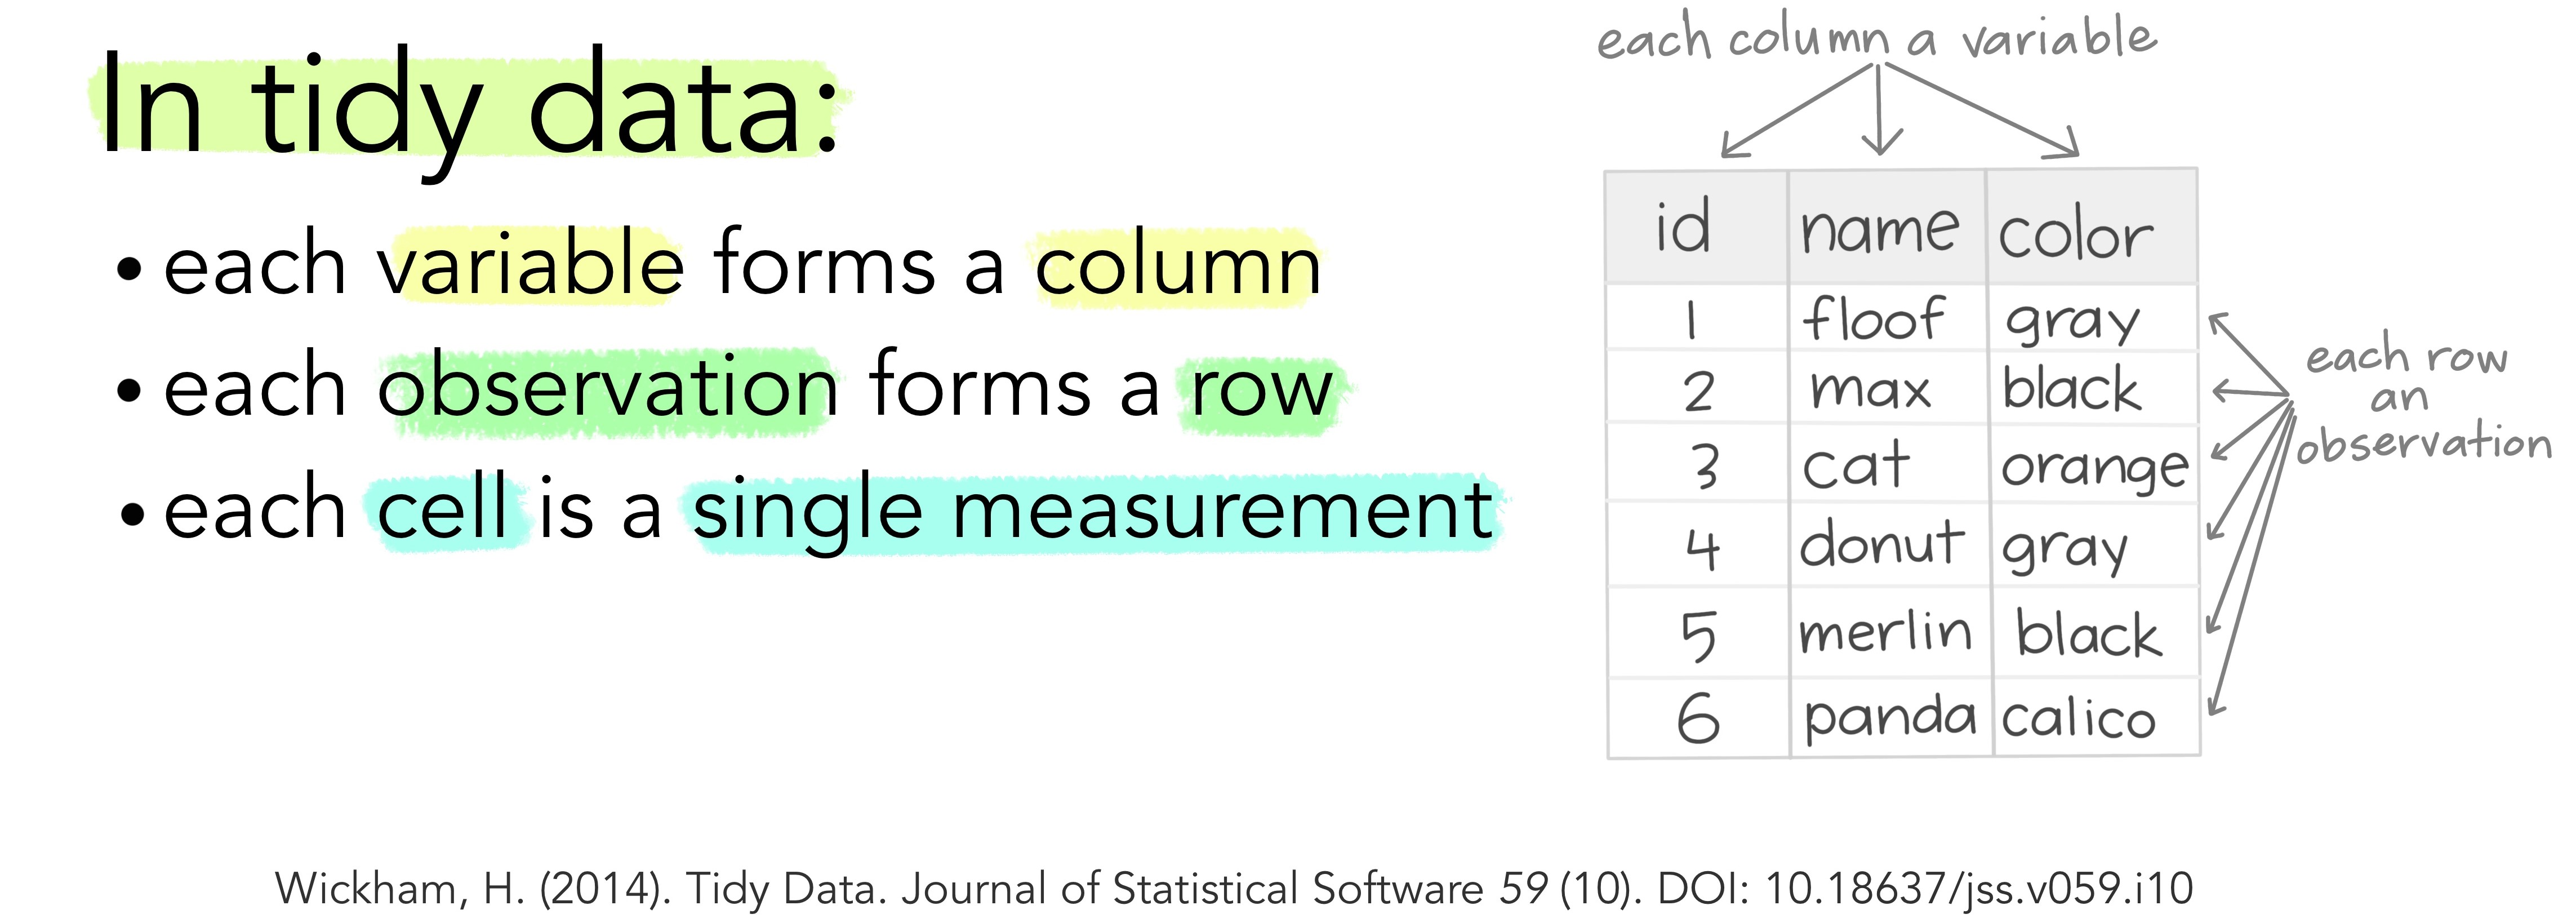
\includegraphics{./Images/tidydata_1.jpg}
\caption{merge}
\end{figure}

Pour passer d'un tableau individu x variable à une structure ordonnée, la fonction pivot\_longer est particulièrement appropriée. En voici l'anatomie.

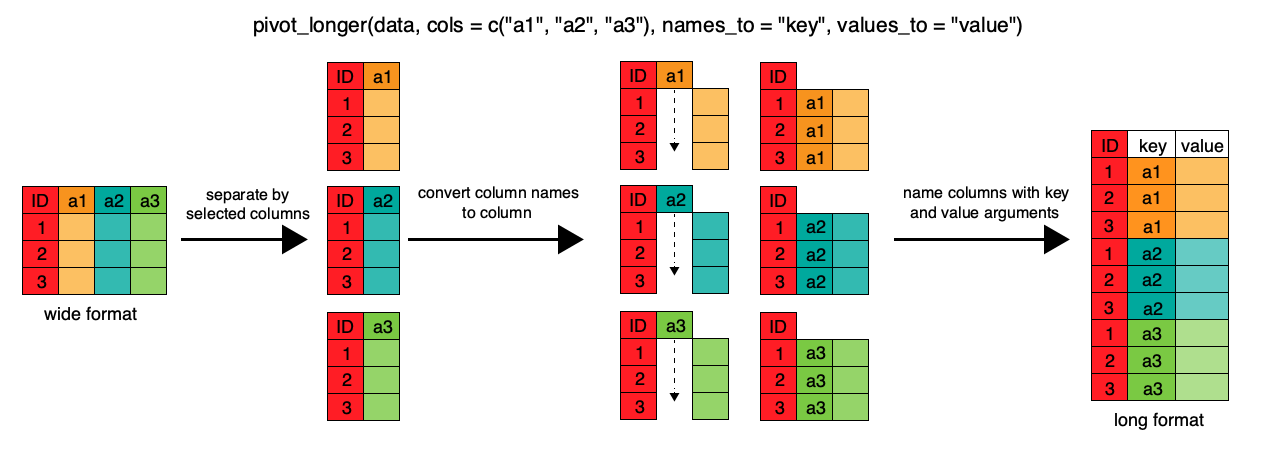
\includegraphics{./Images/pivot_longer.png}
Et un exemple numérique :

\begin{Shaded}
\begin{Highlighting}[]
\NormalTok{foo }\OtherTok{\textless{}{-}}\NormalTok{ foo }\SpecialCharTok{\%\textgreater{}\%}
  \FunctionTok{pivot\_longer}\NormalTok{(}\SpecialCharTok{{-}}\NormalTok{neighbourhood,}\AttributeTok{names\_to=} \StringTok{"Variables"}\NormalTok{,}\AttributeTok{values\_to =} \StringTok{"Values"}\NormalTok{)}

\FunctionTok{ggplot}\NormalTok{(foo, }\FunctionTok{aes}\NormalTok{(}\AttributeTok{x=}\NormalTok{neighbourhood, }\AttributeTok{y=}\NormalTok{Values, }\AttributeTok{group=}\NormalTok{Variables))}\SpecialCharTok{+}
  \FunctionTok{geom\_line}\NormalTok{()}\SpecialCharTok{+}\FunctionTok{facet\_wrap}\NormalTok{(}\FunctionTok{vars}\NormalTok{(Variables),}\AttributeTok{scales=}\StringTok{"free"}\NormalTok{)}\SpecialCharTok{+}
  \FunctionTok{coord\_flip}\NormalTok{()}
\end{Highlighting}
\end{Shaded}

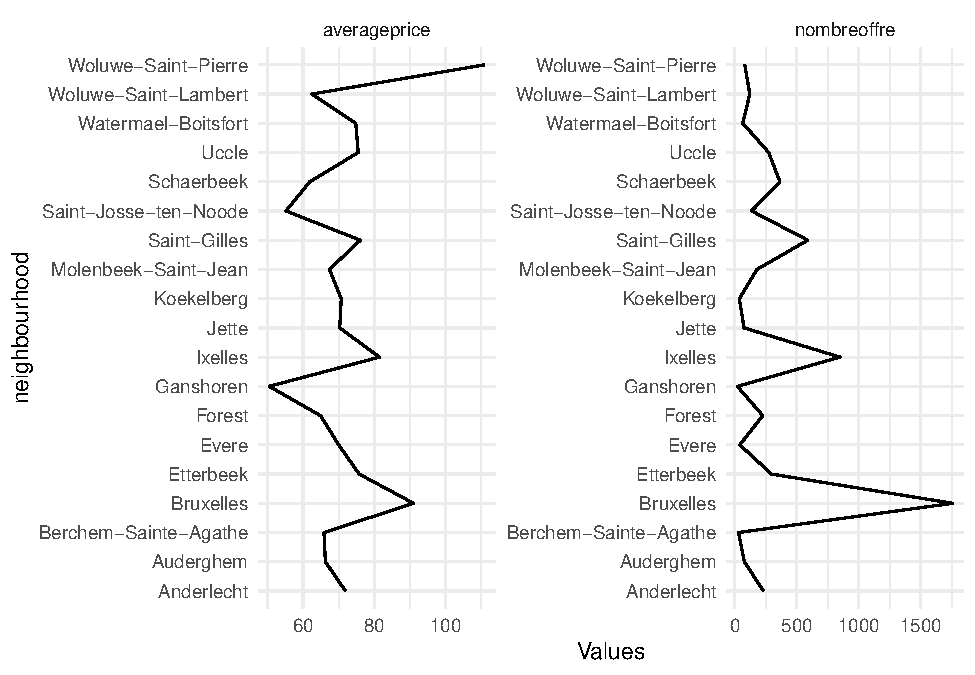
\includegraphics{bookdown-demo_files/figure-latex/0208-1.pdf}

L'opération inverste est de partir d'un tableau long vers un tableau large.
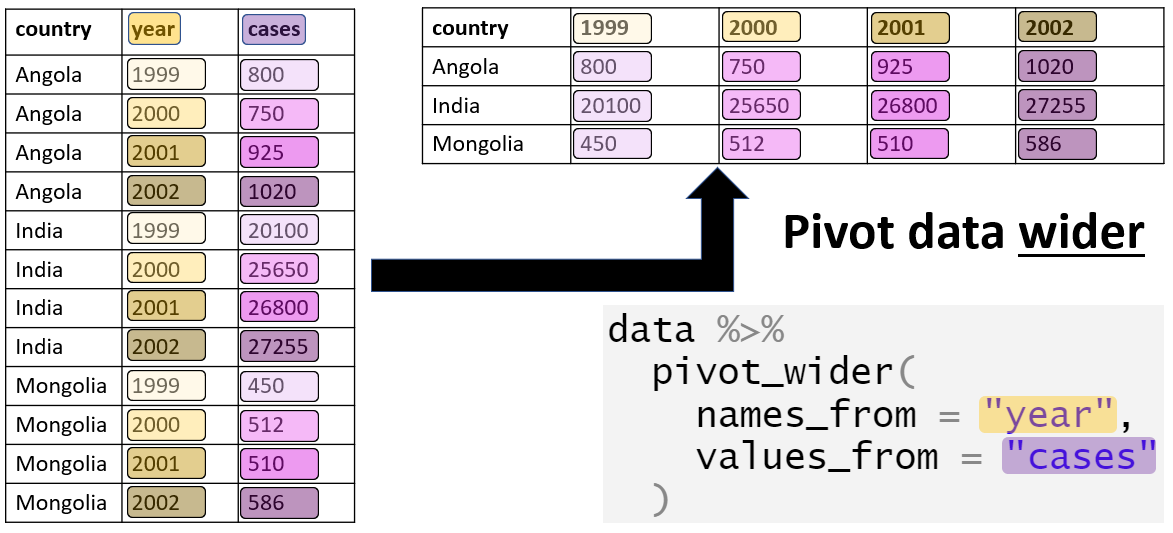
\includegraphics{./Images/pivot_wider.png}

On remarquera que l'usage de cette fonction est nécessaire dans l'emploi de ggplot qui suit la logique des tidy data, ou données ordonnées

\hypertarget{fusionner-les-donnuxe9es}{%
\subsection{Fusionner les données}\label{fusionner-les-donnuxe9es}}

On sera souvent amené à construire des tableaux de données en les enrichissant par d'autres tableaux et à fusionner les données.

Le cas le plus simple est d'ajouter d'autres observations à un fichier de données. On distingue deux cas :

\begin{itemize}
\tightlist
\item
  les deux tableaux concernent les mêmes individus classé dans le même ordre, seules les colonnes diffèrent. On utilisera la fonction \texttt{cbind()}
\item
  si les variables sont identiques mais que les individus sont différents on peut concatène des données avec \texttt{rbind()} (L'équivalent de DPLYR est row\_bind et column\_bind)
\end{itemize}

\begin{Shaded}
\begin{Highlighting}[]
\NormalTok{x1}\OtherTok{\textless{}{-}}\FunctionTok{as.data.frame}\NormalTok{(}\FunctionTok{c}\NormalTok{(}\DecValTok{1}\NormalTok{,}\DecValTok{2}\NormalTok{,}\DecValTok{3}\NormalTok{,}\DecValTok{4}\NormalTok{,}\DecValTok{5}\NormalTok{)) }\SpecialCharTok{\%\textgreater{}\%}\FunctionTok{rename}\NormalTok{(}\AttributeTok{x=}\DecValTok{1}\NormalTok{)}

\NormalTok{y}\OtherTok{\textless{}{-}}\FunctionTok{as.data.frame}\NormalTok{(}\FunctionTok{c}\NormalTok{(}\StringTok{"a"}\NormalTok{,}\StringTok{"b"}\NormalTok{,}\StringTok{"c"}\NormalTok{,}\StringTok{"d"}\NormalTok{,}\StringTok{"e"}\NormalTok{))  }\SpecialCharTok{\%\textgreater{}\%}\FunctionTok{rename}\NormalTok{(}\AttributeTok{y=}\DecValTok{1}\NormalTok{)}

\NormalTok{z}\OtherTok{\textless{}{-}}\FunctionTok{cbind}\NormalTok{(x1,y)}

\NormalTok{ft}\OtherTok{\textless{}{-}}\FunctionTok{flextable}\NormalTok{(z)}
\NormalTok{ft}
\end{Highlighting}
\end{Shaded}

\providecommand{\docline}[3]{\noalign{\global\setlength{\arrayrulewidth}{#1}}\arrayrulecolor[HTML]{#2}\cline{#3}}

\setlength{\tabcolsep}{2pt}

\renewcommand*{\arraystretch}{1.5}

\begin{longtable}[c]{|p{0.75in}|p{0.75in}}



\hhline{>{\arrayrulecolor[HTML]{666666}\global\arrayrulewidth=2pt}->{\arrayrulecolor[HTML]{666666}\global\arrayrulewidth=2pt}-}

\multicolumn{1}{!{\color[HTML]{000000}\vrule width 0pt}>{\raggedleft}p{\dimexpr 0.75in+0\tabcolsep+0\arrayrulewidth}}{\fontsize{11}{11}\selectfont{\textcolor[HTML]{000000}{\global\setmainfont{Arial}{x}}}} & \multicolumn{1}{!{\color[HTML]{000000}\vrule width 0pt}>{\raggedright}p{\dimexpr 0.75in+0\tabcolsep+0\arrayrulewidth}!{\color[HTML]{000000}\vrule width 0pt}}{\fontsize{11}{11}\selectfont{\textcolor[HTML]{000000}{\global\setmainfont{Arial}{y}}}} \\

\noalign{\global\setlength{\arrayrulewidth}{2pt}}\arrayrulecolor[HTML]{666666}\cline{1-2}

\endfirsthead

\hhline{>{\arrayrulecolor[HTML]{666666}\global\arrayrulewidth=2pt}->{\arrayrulecolor[HTML]{666666}\global\arrayrulewidth=2pt}-}

\multicolumn{1}{!{\color[HTML]{000000}\vrule width 0pt}>{\raggedleft}p{\dimexpr 0.75in+0\tabcolsep+0\arrayrulewidth}}{\fontsize{11}{11}\selectfont{\textcolor[HTML]{000000}{\global\setmainfont{Arial}{x}}}} & \multicolumn{1}{!{\color[HTML]{000000}\vrule width 0pt}>{\raggedright}p{\dimexpr 0.75in+0\tabcolsep+0\arrayrulewidth}!{\color[HTML]{000000}\vrule width 0pt}}{\fontsize{11}{11}\selectfont{\textcolor[HTML]{000000}{\global\setmainfont{Arial}{y}}}} \\

\noalign{\global\setlength{\arrayrulewidth}{2pt}}\arrayrulecolor[HTML]{666666}\cline{1-2}\endhead



\multicolumn{1}{!{\color[HTML]{000000}\vrule width 0pt}>{\raggedleft}p{\dimexpr 0.75in+0\tabcolsep+0\arrayrulewidth}}{\fontsize{11}{11}\selectfont{\textcolor[HTML]{000000}{\global\setmainfont{Arial}{1}}}} & \multicolumn{1}{!{\color[HTML]{000000}\vrule width 0pt}>{\raggedright}p{\dimexpr 0.75in+0\tabcolsep+0\arrayrulewidth}!{\color[HTML]{000000}\vrule width 0pt}}{\fontsize{11}{11}\selectfont{\textcolor[HTML]{000000}{\global\setmainfont{Arial}{a}}}} \\





\multicolumn{1}{!{\color[HTML]{000000}\vrule width 0pt}>{\raggedleft}p{\dimexpr 0.75in+0\tabcolsep+0\arrayrulewidth}}{\fontsize{11}{11}\selectfont{\textcolor[HTML]{000000}{\global\setmainfont{Arial}{2}}}} & \multicolumn{1}{!{\color[HTML]{000000}\vrule width 0pt}>{\raggedright}p{\dimexpr 0.75in+0\tabcolsep+0\arrayrulewidth}!{\color[HTML]{000000}\vrule width 0pt}}{\fontsize{11}{11}\selectfont{\textcolor[HTML]{000000}{\global\setmainfont{Arial}{b}}}} \\





\multicolumn{1}{!{\color[HTML]{000000}\vrule width 0pt}>{\raggedleft}p{\dimexpr 0.75in+0\tabcolsep+0\arrayrulewidth}}{\fontsize{11}{11}\selectfont{\textcolor[HTML]{000000}{\global\setmainfont{Arial}{3}}}} & \multicolumn{1}{!{\color[HTML]{000000}\vrule width 0pt}>{\raggedright}p{\dimexpr 0.75in+0\tabcolsep+0\arrayrulewidth}!{\color[HTML]{000000}\vrule width 0pt}}{\fontsize{11}{11}\selectfont{\textcolor[HTML]{000000}{\global\setmainfont{Arial}{c}}}} \\





\multicolumn{1}{!{\color[HTML]{000000}\vrule width 0pt}>{\raggedleft}p{\dimexpr 0.75in+0\tabcolsep+0\arrayrulewidth}}{\fontsize{11}{11}\selectfont{\textcolor[HTML]{000000}{\global\setmainfont{Arial}{4}}}} & \multicolumn{1}{!{\color[HTML]{000000}\vrule width 0pt}>{\raggedright}p{\dimexpr 0.75in+0\tabcolsep+0\arrayrulewidth}!{\color[HTML]{000000}\vrule width 0pt}}{\fontsize{11}{11}\selectfont{\textcolor[HTML]{000000}{\global\setmainfont{Arial}{d}}}} \\





\multicolumn{1}{!{\color[HTML]{000000}\vrule width 0pt}>{\raggedleft}p{\dimexpr 0.75in+0\tabcolsep+0\arrayrulewidth}}{\fontsize{11}{11}\selectfont{\textcolor[HTML]{000000}{\global\setmainfont{Arial}{5}}}} & \multicolumn{1}{!{\color[HTML]{000000}\vrule width 0pt}>{\raggedright}p{\dimexpr 0.75in+0\tabcolsep+0\arrayrulewidth}!{\color[HTML]{000000}\vrule width 0pt}}{\fontsize{11}{11}\selectfont{\textcolor[HTML]{000000}{\global\setmainfont{Arial}{e}}}} \\

\noalign{\global\setlength{\arrayrulewidth}{2pt}}\arrayrulecolor[HTML]{666666}\cline{1-2}



\end{longtable}

\begin{Shaded}
\begin{Highlighting}[]
\NormalTok{x2}\OtherTok{\textless{}{-}}\FunctionTok{as.data.frame}\NormalTok{(}\FunctionTok{c}\NormalTok{(}\DecValTok{9}\NormalTok{,}\DecValTok{8}\NormalTok{,}\DecValTok{7}\NormalTok{,}\DecValTok{6}\NormalTok{)) }\SpecialCharTok{\%\textgreater{}\%}\FunctionTok{rename}\NormalTok{(}\AttributeTok{x=}\DecValTok{1}\NormalTok{)}

\NormalTok{w}\OtherTok{\textless{}{-}}\FunctionTok{rbind}\NormalTok{(x1,x2)}

\NormalTok{ft}\OtherTok{\textless{}{-}}\FunctionTok{flextable}\NormalTok{(w)}
\NormalTok{ft}
\end{Highlighting}
\end{Shaded}

\providecommand{\docline}[3]{\noalign{\global\setlength{\arrayrulewidth}{#1}}\arrayrulecolor[HTML]{#2}\cline{#3}}

\setlength{\tabcolsep}{2pt}

\renewcommand*{\arraystretch}{1.5}

\begin{longtable}[c]{|p{0.75in}}



\hhline{>{\arrayrulecolor[HTML]{666666}\global\arrayrulewidth=2pt}-}

\multicolumn{1}{!{\color[HTML]{000000}\vrule width 0pt}>{\raggedleft}p{\dimexpr 0.75in+0\tabcolsep+0\arrayrulewidth}!{\color[HTML]{000000}\vrule width 0pt}}{\fontsize{11}{11}\selectfont{\textcolor[HTML]{000000}{\global\setmainfont{Arial}{x}}}} \\

\noalign{\global\setlength{\arrayrulewidth}{2pt}}\arrayrulecolor[HTML]{666666}\cline{1-1}

\endfirsthead

\hhline{>{\arrayrulecolor[HTML]{666666}\global\arrayrulewidth=2pt}-}

\multicolumn{1}{!{\color[HTML]{000000}\vrule width 0pt}>{\raggedleft}p{\dimexpr 0.75in+0\tabcolsep+0\arrayrulewidth}!{\color[HTML]{000000}\vrule width 0pt}}{\fontsize{11}{11}\selectfont{\textcolor[HTML]{000000}{\global\setmainfont{Arial}{x}}}} \\

\noalign{\global\setlength{\arrayrulewidth}{2pt}}\arrayrulecolor[HTML]{666666}\cline{1-1}\endhead



\multicolumn{1}{!{\color[HTML]{000000}\vrule width 0pt}>{\raggedleft}p{\dimexpr 0.75in+0\tabcolsep+0\arrayrulewidth}!{\color[HTML]{000000}\vrule width 0pt}}{\fontsize{11}{11}\selectfont{\textcolor[HTML]{000000}{\global\setmainfont{Arial}{1}}}} \\





\multicolumn{1}{!{\color[HTML]{000000}\vrule width 0pt}>{\raggedleft}p{\dimexpr 0.75in+0\tabcolsep+0\arrayrulewidth}!{\color[HTML]{000000}\vrule width 0pt}}{\fontsize{11}{11}\selectfont{\textcolor[HTML]{000000}{\global\setmainfont{Arial}{2}}}} \\





\multicolumn{1}{!{\color[HTML]{000000}\vrule width 0pt}>{\raggedleft}p{\dimexpr 0.75in+0\tabcolsep+0\arrayrulewidth}!{\color[HTML]{000000}\vrule width 0pt}}{\fontsize{11}{11}\selectfont{\textcolor[HTML]{000000}{\global\setmainfont{Arial}{3}}}} \\





\multicolumn{1}{!{\color[HTML]{000000}\vrule width 0pt}>{\raggedleft}p{\dimexpr 0.75in+0\tabcolsep+0\arrayrulewidth}!{\color[HTML]{000000}\vrule width 0pt}}{\fontsize{11}{11}\selectfont{\textcolor[HTML]{000000}{\global\setmainfont{Arial}{4}}}} \\





\multicolumn{1}{!{\color[HTML]{000000}\vrule width 0pt}>{\raggedleft}p{\dimexpr 0.75in+0\tabcolsep+0\arrayrulewidth}!{\color[HTML]{000000}\vrule width 0pt}}{\fontsize{11}{11}\selectfont{\textcolor[HTML]{000000}{\global\setmainfont{Arial}{5}}}} \\





\multicolumn{1}{!{\color[HTML]{000000}\vrule width 0pt}>{\raggedleft}p{\dimexpr 0.75in+0\tabcolsep+0\arrayrulewidth}!{\color[HTML]{000000}\vrule width 0pt}}{\fontsize{11}{11}\selectfont{\textcolor[HTML]{000000}{\global\setmainfont{Arial}{9}}}} \\





\multicolumn{1}{!{\color[HTML]{000000}\vrule width 0pt}>{\raggedleft}p{\dimexpr 0.75in+0\tabcolsep+0\arrayrulewidth}!{\color[HTML]{000000}\vrule width 0pt}}{\fontsize{11}{11}\selectfont{\textcolor[HTML]{000000}{\global\setmainfont{Arial}{8}}}} \\





\multicolumn{1}{!{\color[HTML]{000000}\vrule width 0pt}>{\raggedleft}p{\dimexpr 0.75in+0\tabcolsep+0\arrayrulewidth}!{\color[HTML]{000000}\vrule width 0pt}}{\fontsize{11}{11}\selectfont{\textcolor[HTML]{000000}{\global\setmainfont{Arial}{7}}}} \\





\multicolumn{1}{!{\color[HTML]{000000}\vrule width 0pt}>{\raggedleft}p{\dimexpr 0.75in+0\tabcolsep+0\arrayrulewidth}!{\color[HTML]{000000}\vrule width 0pt}}{\fontsize{11}{11}\selectfont{\textcolor[HTML]{000000}{\global\setmainfont{Arial}{6}}}} \\

\noalign{\global\setlength{\arrayrulewidth}{2pt}}\arrayrulecolor[HTML]{666666}\cline{1-1}



\end{longtable}

mais très souvent on sera dans des cas différents et la fusion des données devra suivre des index

\begin{figure}
\centering
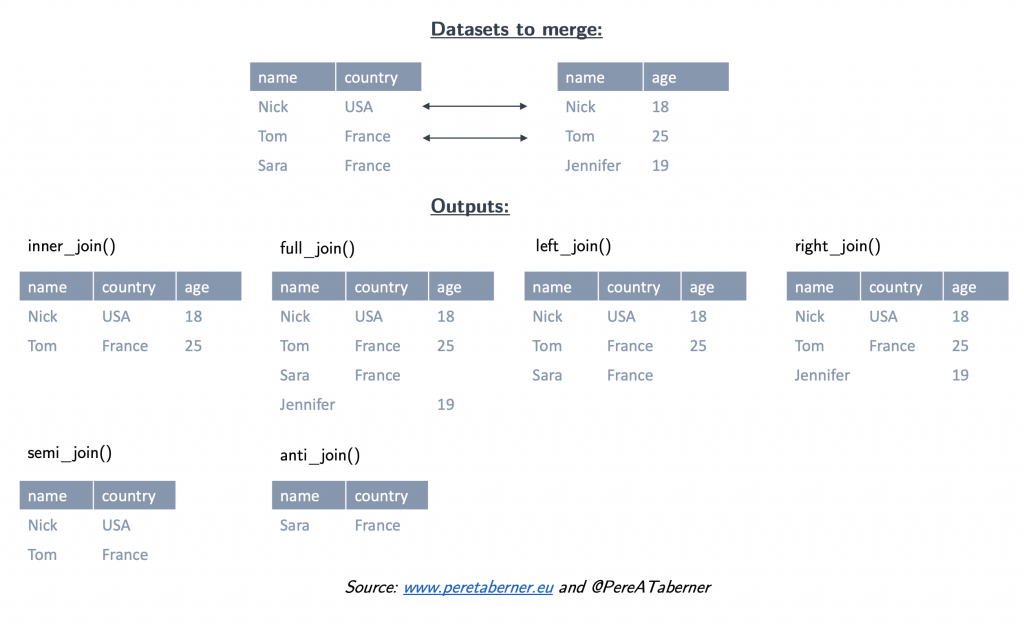
\includegraphics{./Images/merge_ex-1024x624.png}
\caption{merge}
\end{figure}

Plusieurs types de fusion sont proposées.

\begin{figure}
\centering
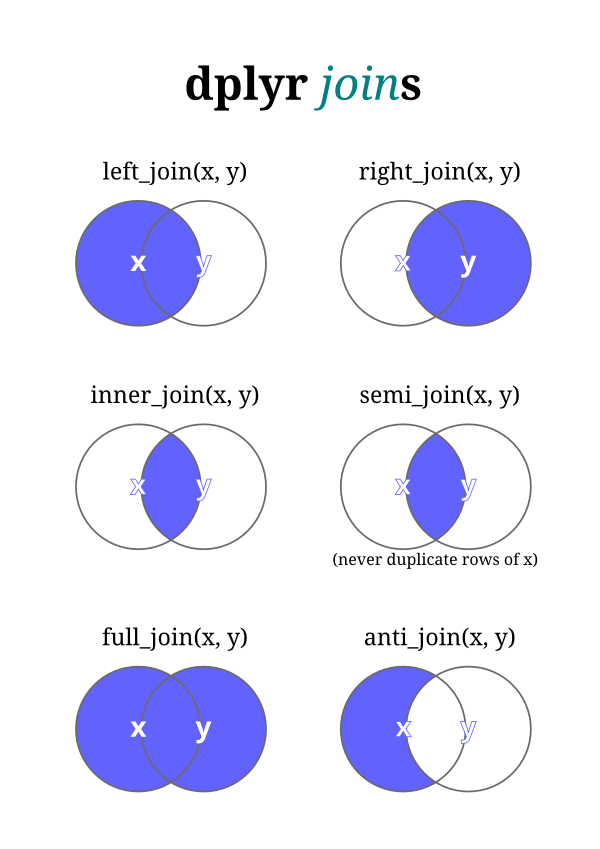
\includegraphics{./Images/join_diagram.png}
\caption{Mode de fusions}
\end{figure}

genérale

fusion à gauche

fusion à droite

(Voir ce cours){[}\url{https://coletl.github.io/tidy_intro/lessons/dplyr_join/dplyr_join.html}{]}

\hypertarget{introduction-uxe0-la-grammaire-des-graphiques-et-uxe0-ggplot}{%
\chapter{Introduction à la grammaire des graphiques et à ggplot}\label{introduction-uxe0-la-grammaire-des-graphiques-et-uxe0-ggplot}}

Nous avons appris à lire des données, à les manipuler, Nous allons nous intéresser à la manière de les représenter en introduisant le concept de grammaire des graphiques et en appliquant ggplot au traitement des données univariées.

\hypertarget{la-grammaire-des-graphiques}{%
\section{La grammaire des graphiques}\label{la-grammaire-des-graphiques}}

C'est sans doute une des percées conceptuelles la plus intéressante des data sciences. La représentation graphiques des données fait l'objet à la fois d'une explosion créative mais aussi d'une synthèse théorique. C'est l'apport de la grammaire des graphiques.

Ces outils s'appuient sur l'idée de \href{https://www.goodreads.com/book/show/2549408.The_Grammar_of_Graphics}{grammaire des graphiques}. En voici un \href{https://cfss.uchicago.edu/notes/grammar-of-graphics/}{clair résumé}.En français il y a toujours le \href{http://larmarange.github.io/analyse-R/intro-ggplot2.html}{larmarange}

\hypertarget{un-moduxe8le-en-couche}{%
\subsection{Un modèle en couche}\label{un-moduxe8le-en-couche}}

Celle-ci met un ordre dans les éléments qui composent un graphique et les superpose.

\begin{figure}
\centering

\includegraphics{./Images/graphiclayers.png}
\caption{layers}
\end{figure}

\begin{itemize}
\tightlist
\item
  l'aesthetic definit les éléments que l'on veut représenter : ce qu'on met en abscisse, ce qu'on met en ordonnné, les groupes que l'on veut distinguer.
\item
  la geométrie (geom\_x)qui définit la forme de représentation
\item
  les échelles (scale\_x)
\item
  Labelisation (labs)
\item
  les templates
\item
  le facetting
\end{itemize}

ggplot est construit selon cette structure. Voici le \href{https://ggplot2-book.org/}{book de référence}, qui est au centre de ce cours. On aura besoin de manière assez systématique de manipuler les données avant de les représenter, \href{http://larmarange.github.io/analyse-R/manipuler-les-donnees-avec-dplyr.html}{dplyr} nous permet de le faire aisément.

\hypertarget{une-typologie-des-repruxe9sentations}{%
\subsection{Une typologie des représentations}\label{une-typologie-des-repruxe9sentations}}

Un point de départ fondamental est la \href{https://www.r-graph-gallery.com/}{gallery de ggplot},, elle présente de manière synthétique la plupart les types de figures qui peuvent être représentées, avec du code facilement reproductible.

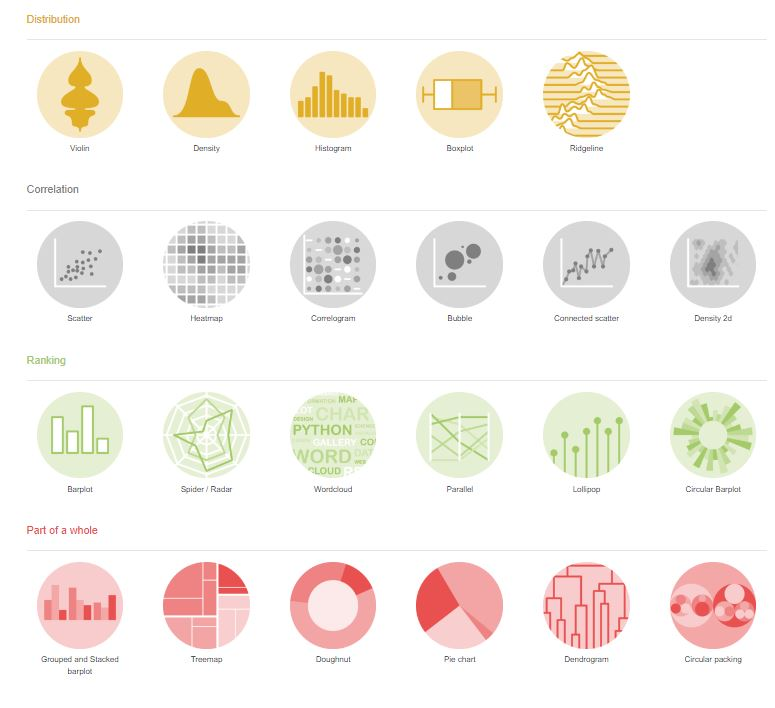
\includegraphics{./Images/ggplotGallery1.jpg}
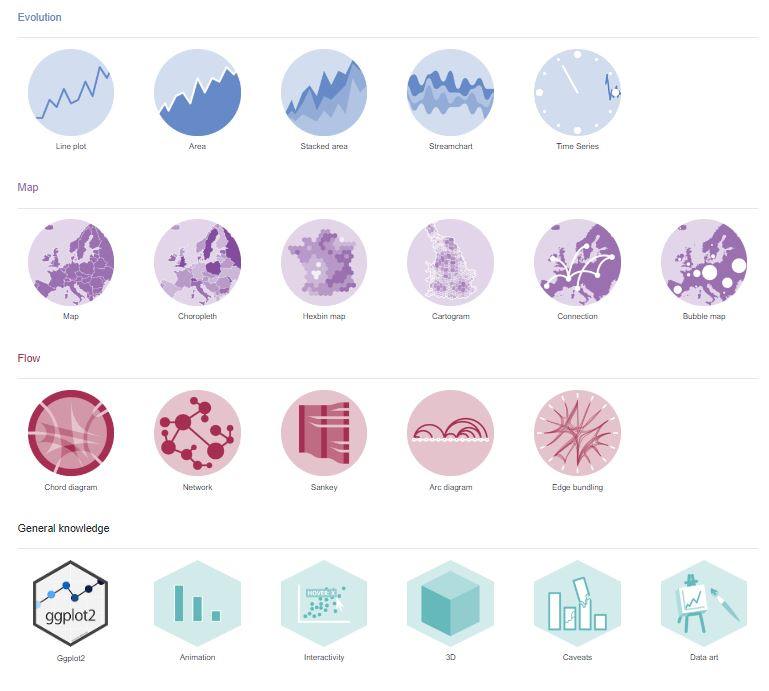
\includegraphics{./Images/ggplotGallery2.jpg}
Une classification simple

\begin{itemize}
\tightlist
\item
  Analyse univariée : une seule variable quantitative ou qualitative.
\item
  Analyse bivariée : deux variables quali ou quanti/
\item
  Analyse multivariée

  \begin{itemize}
  \tightlist
  \item
    les variables sont quantitatives : on analyse des matrices de corrélations
  \item
    les variables sont qualitatives : on analyse des tableaux croisés
  \end{itemize}
\item
  Analyse temporelles :
\item
  Analyse géospatiale : les chloroplèthes.
\item
  Analyse de réseaux : représenter des noeuds et les arcs qui les relient. Depuis Moreno,
\item
  analyse d'arbres : ils sont des sortes de réseaux mais avec une structure hiérarchiques. le dendogramme est le plus connus.
\item
  Diagramme de flux
\end{itemize}

\hypertarget{lesthuxe9tique}{%
\subsection{L'esthétique}\label{lesthuxe9tique}}

L'art des couleurs tient dans les palettes on aimera celles de \href{https://github.com/karthik/wesanderson}{Wes Anderson}, on peut adorer \href{https://nschiett.github.io/fishualize/index.html}{\texttt{fishualize}} si on a un faible pour les poissons tropicaux.

Pour la théorie voir \ldots{}

Si l'on est pas créatif on se reportera à des modèles, certains étant fameux. On laisse le lecteur les rechercher ici ou là . A titre d'exemple, \href{https://rpubs.com/ysittaa/BMIsitta}{une belle leçon}, pour reproduire le célèbre \href{https://www.economist.com/big-mac-index}{BigMac index} de The Economist.

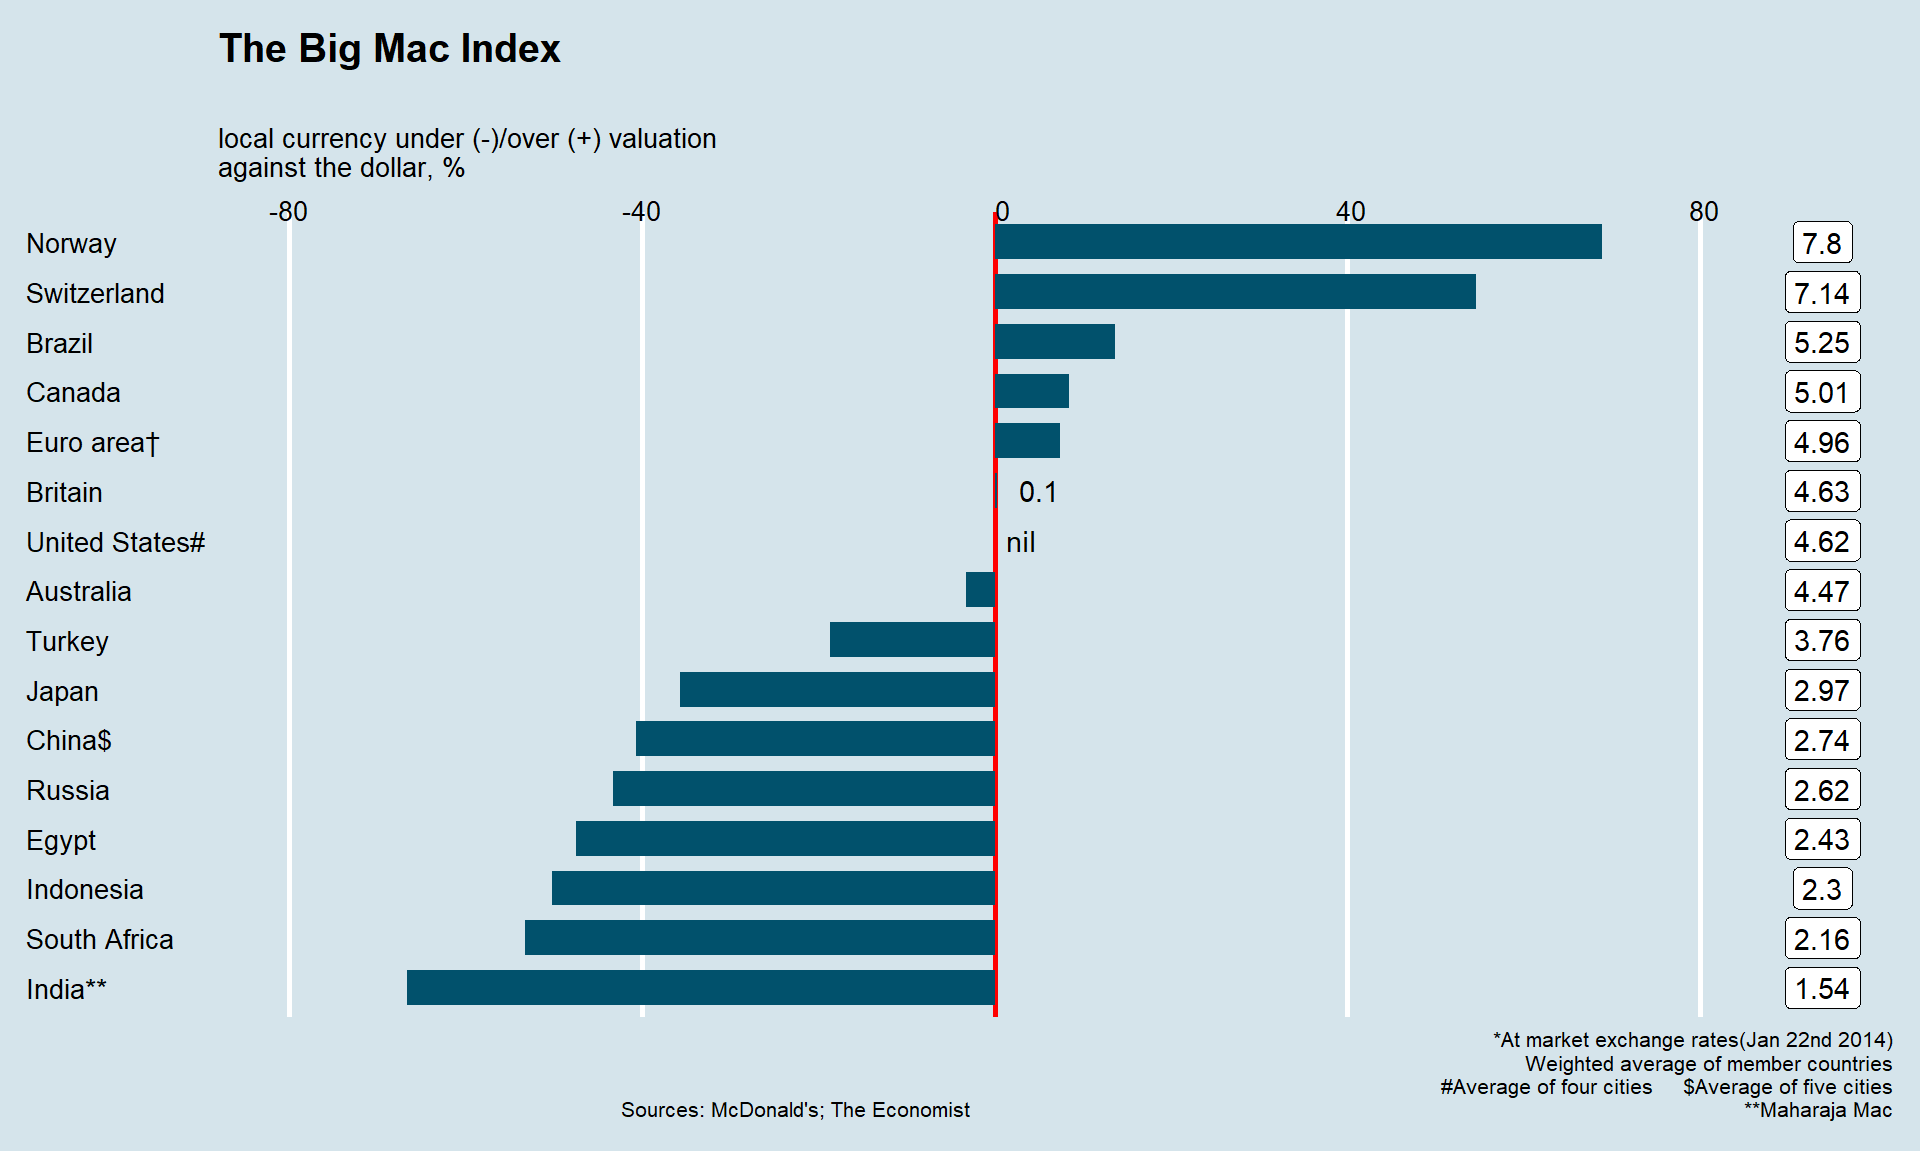
\includegraphics{./Images/Bigmacindex.png}
\#\# Application à l'analyse univariée

Les données sont extraites de l'ESS, une sélection est disponible \href{}{ici}. Elle couvre les 9 vagues et concernent la France et L'Allemagne. Les variables dépendantes (celles que l'on veut étudier et expliquer) sont les 9 items de la confiance, les variable considérées comme indépendantes (ou explicatives) sont une sélection de variables socio-démographiques : âge, genre, perception du pouvoir d'achat, orientation politique, type d'habitat.

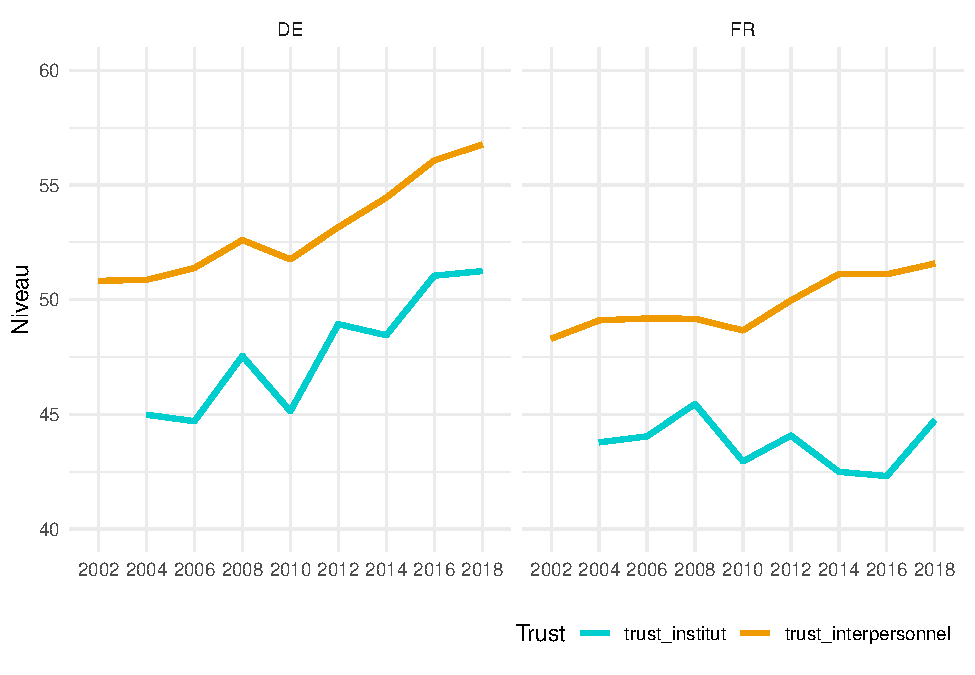
\includegraphics{bookdown-demo_files/figure-latex/301-1.pdf}
L'analyse univarié, comme son nom l'indique, ne s'intéresse qu'à une seule variable. Celle-ci peut être \textbf{quantitative} ou \textbf{qualitative} et ne comporter qu'un nombre limité de modalités entre lesquels aucune comparaison de grandeur ne peut être faite. Les premières ont le plus souvent dans r un format numérique, les autres correspondent au format \emph{factor}.

\hypertarget{le-cas-des-variables-quantitatives}{%
\subsection{Le cas des variables quantitatives}\label{le-cas-des-variables-quantitatives}}

Les variables quantitatives décrivent une variable dont les valeurs décrivent les quantités d'une grandeur. Elle peuvent être discrètes (dénombrement du d'un nombre d'unités) - le nombre d'habitant), ou continue (le nombre de km parcourus). l'\textbf{histogramme} est l'outil de base pour représenter la distribution d'une telle variable. Il représente pour des intervalles de valeurs donnés, la fréquence des observations.

Sa syntaxe simple comporte d'abord la définition de la variable et de la source de données, puis une des ``géométrie'' de ggplot : la fonction \texttt{geom\_histogram}. Dans notre exemple, on va représenter le score de confiance institutionnelle pour la France en se concentrant sur la dernière vague d'enquête.

\begin{Shaded}
\begin{Highlighting}[]
\NormalTok{df}\OtherTok{\textless{}{-}}\FunctionTok{readRDS}\NormalTok{(}\StringTok{"./data/dfTrust.rds)"}\NormalTok{)}

\CommentTok{\#filtrage sur 2018 et la France.}

\NormalTok{foo}\OtherTok{\textless{}{-}}\NormalTok{df}\SpecialCharTok{\%\textgreater{}\%}
  \FunctionTok{filter}\NormalTok{(Year}\SpecialCharTok{==}\StringTok{"2018"} \SpecialCharTok{\&}\NormalTok{ cntry}\SpecialCharTok{==}\StringTok{"FR"} \SpecialCharTok{\&} \SpecialCharTok{!}\FunctionTok{is.na}\NormalTok{(trust\_institut)) }

\CommentTok{\# on stocke le diagramme dans l\textquotesingle{}objet g00, }
\CommentTok{\# pour le réutiliser ultérieurement et pouvoir le compléter.}

\NormalTok{g00}\OtherTok{\textless{}{-}}\FunctionTok{ggplot}\NormalTok{(foo,}\FunctionTok{aes}\NormalTok{(}\AttributeTok{x=}\NormalTok{trust\_institut))}\SpecialCharTok{+}
  \FunctionTok{geom\_histogram}\NormalTok{()}

\NormalTok{g00}
\end{Highlighting}
\end{Shaded}

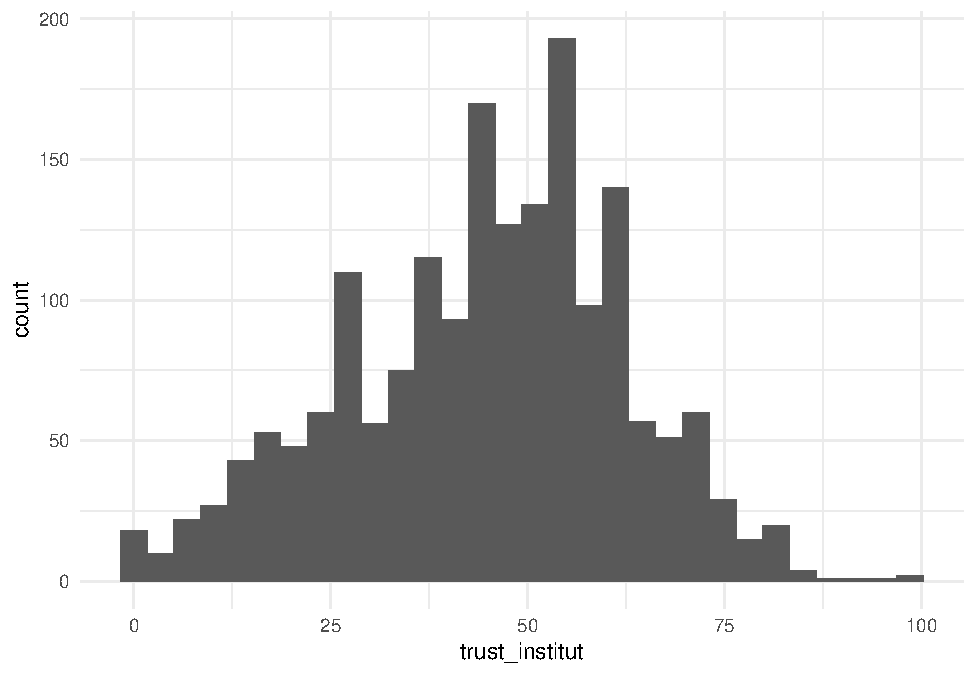
\includegraphics{bookdown-demo_files/figure-latex/302-1.pdf}

\begin{Shaded}
\begin{Highlighting}[]
\NormalTok{g00}\SpecialCharTok{+}\FunctionTok{labs}\NormalTok{(}\AttributeTok{title=}\StringTok{"Distribution de la confiance institutionnelle en France et en 2018"}\NormalTok{,}
         \AttributeTok{x=}\StringTok{"Confiance institutionnelle"}\NormalTok{, }\AttributeTok{y=}\StringTok{"Fréquence"}\NormalTok{)}
\end{Highlighting}
\end{Shaded}

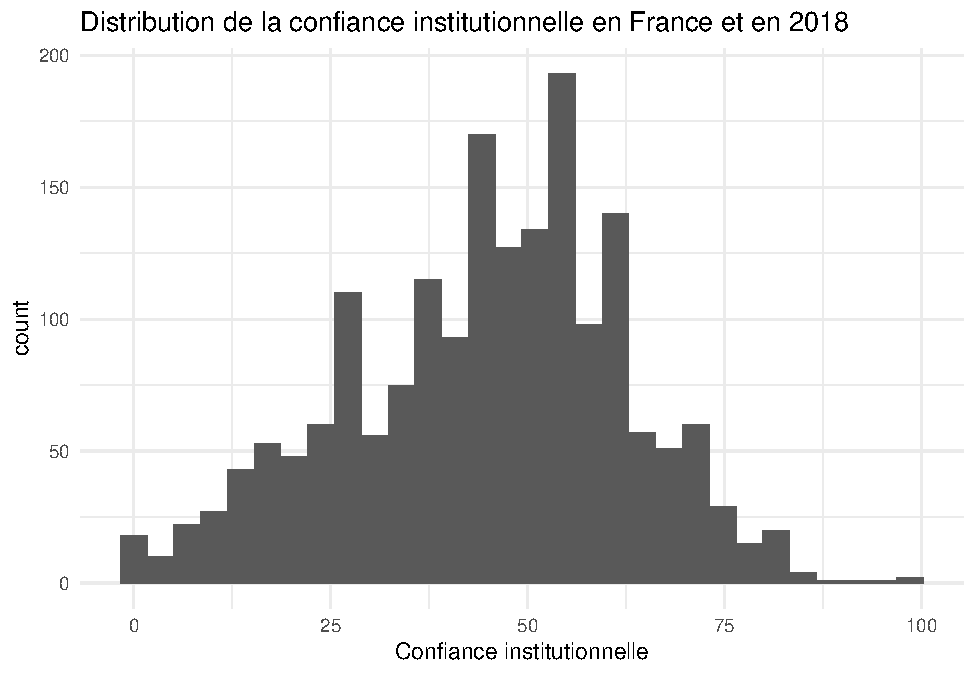
\includegraphics{bookdown-demo_files/figure-latex/302-2.pdf}

On va améliorer l'aspect en

\begin{enumerate}
\def\labelenumi{\arabic{enumi}.}
\tightlist
\item
  modifiant la couleur et la largeur des barres,
\item
  ajoutant un thème,
\item
  en précisant les éléments textuels (titres, label)
\item
  en calculant et en représentant la valeur moyenne et l'écart-type . Pour ces statistiques, on emploie les fonction de base : mean, sd et round.
\end{enumerate}

On notera que le titre est défini par la concaténation de plusieurs chaines de caractères avec la fonction \texttt{paste0}. On peut ainsi injecter dans le graphique des éléments externes au jeu de données.

\begin{Shaded}
\begin{Highlighting}[]
\CommentTok{\#on calcule la moyenne}
\NormalTok{moy}\OtherTok{=}\FunctionTok{mean}\NormalTok{(foo}\SpecialCharTok{$}\NormalTok{trust\_institut, }\AttributeTok{na.rm=}\ConstantTok{TRUE}\NormalTok{)}
\NormalTok{sd}\OtherTok{=}\FunctionTok{sd}\NormalTok{(foo}\SpecialCharTok{$}\NormalTok{trust\_institut, }\AttributeTok{na.rm=}\ConstantTok{TRUE}\NormalTok{)}

\CommentTok{\#avec tous les éléments}
\NormalTok{g01 }\OtherTok{\textless{}{-}}\FunctionTok{ggplot}\NormalTok{(foo,}\FunctionTok{aes}\NormalTok{(}\AttributeTok{x=}\NormalTok{trust\_institut))}\SpecialCharTok{+}
  \FunctionTok{geom\_histogram}\NormalTok{(}\AttributeTok{binwidth=}\DecValTok{5}\NormalTok{,}\AttributeTok{fill=}\StringTok{"pink"}\NormalTok{)}\SpecialCharTok{+}
  \FunctionTok{labs}\NormalTok{(}\AttributeTok{title=} \StringTok{"Distribution de la confiance institutionnelle"}\NormalTok{, }
       \AttributeTok{subtitle=} \FunctionTok{paste0}\NormalTok{(}\StringTok{"moyenne = "}\NormalTok{,}\FunctionTok{round}\NormalTok{(moy,}\DecValTok{2}\NormalTok{), }\StringTok{" {-} écart{-}type = "}\NormalTok{, }\FunctionTok{round}\NormalTok{(sd,}\DecValTok{2}\NormalTok{)),}
       \AttributeTok{caption=}\StringTok{"ESS2002{-}2018"}\NormalTok{,}
       \AttributeTok{y=} \StringTok{"Fréquence"}\NormalTok{,}
       \AttributeTok{x=}\StringTok{"Confiance (index de 0 à 100)"}\NormalTok{)}\SpecialCharTok{+}
    \FunctionTok{geom\_vline}\NormalTok{(}\AttributeTok{xintercept=}\NormalTok{moy, }\AttributeTok{color=}\StringTok{"red"}\NormalTok{,}\AttributeTok{size=}\FloatTok{1.5}\NormalTok{)}\SpecialCharTok{+}
        \FunctionTok{geom\_segment}\NormalTok{(}\AttributeTok{y =} \DecValTok{0}\NormalTok{, }\AttributeTok{yend=}\DecValTok{0}\NormalTok{,}\AttributeTok{x=}\NormalTok{moy}\SpecialCharTok{{-}}\NormalTok{sd,}\AttributeTok{xend=}\NormalTok{moy}\SpecialCharTok{+}\NormalTok{sd, }\AttributeTok{color=}\StringTok{"orange"}\NormalTok{,}\AttributeTok{size=}\FloatTok{1.5}\NormalTok{)}

\NormalTok{g01}
\end{Highlighting}
\end{Shaded}

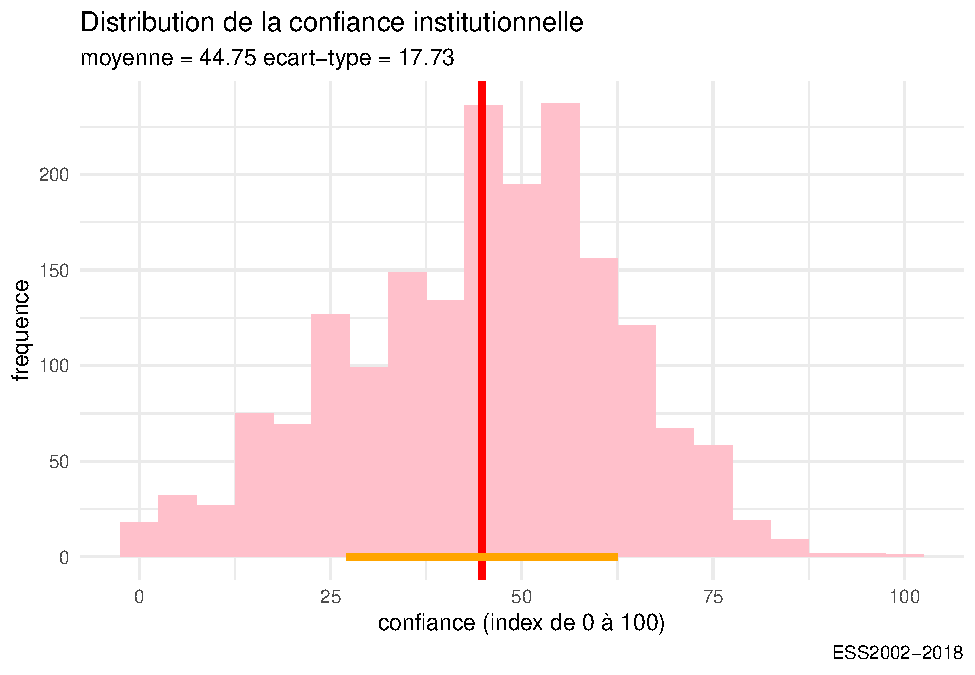
\includegraphics{bookdown-demo_files/figure-latex/303-1.pdf}

On peut souhaiter normaliser un tel graphe et prendre pour convention que la surface soit égale à 1. On représentera donc une fonction de densité de probabilité, à laquelle on peut associer une fonction cumulée de la distribution.

On en profite pour introduire l'usage de \href{https://cran.r-project.org/web/packages/cowplot/vignettes/introduction.html}{\texttt{cowplot}} qui permet d'associer des graphiques en un seul document.

\begin{Shaded}
\begin{Highlighting}[]
\NormalTok{g04}\OtherTok{\textless{}{-}}\FunctionTok{ggplot}\NormalTok{(foo,}\FunctionTok{aes}\NormalTok{(}\AttributeTok{x=}\NormalTok{trust\_institut))}\SpecialCharTok{+} 
  \FunctionTok{geom\_density}\NormalTok{(}\AttributeTok{fill=}\StringTok{"pink2"}\NormalTok{) }\SpecialCharTok{+}
  \FunctionTok{labs}\NormalTok{(}\AttributeTok{title=} \StringTok{"Fonction de densité de probabilité"}\NormalTok{, }
       \AttributeTok{caption=}\StringTok{"ESS2002{-}2018"}\NormalTok{,}
       \AttributeTok{y=} \StringTok{"Fréquence"}\NormalTok{,}
       \AttributeTok{x=}\StringTok{"Confiance (index de 1 à 100)"}\NormalTok{) }

\NormalTok{g05}\OtherTok{\textless{}{-}}\FunctionTok{ggplot}\NormalTok{(foo,}\FunctionTok{aes}\NormalTok{(}\AttributeTok{x=}\NormalTok{trust\_institut))}\SpecialCharTok{+} 
  \FunctionTok{stat\_ecdf}\NormalTok{(}\AttributeTok{geom =} \StringTok{"step"}\NormalTok{)}\SpecialCharTok{+}
  \FunctionTok{labs}\NormalTok{(}\AttributeTok{title=} \StringTok{"Fonction de distribution empirique cumulée"}\NormalTok{, }
       \AttributeTok{caption=}\StringTok{"ESS2002{-}2018"}\NormalTok{,}
       \AttributeTok{y=} \StringTok{"Fréquence"}\NormalTok{,}
       \AttributeTok{x=}\StringTok{"Confiance (index de 1 à 100)"}\NormalTok{) }

\FunctionTok{plot\_grid}\NormalTok{(g04, g05, }\AttributeTok{labels =} \FunctionTok{c}\NormalTok{(}\StringTok{\textquotesingle{}A\textquotesingle{}}\NormalTok{, }\StringTok{\textquotesingle{}B\textquotesingle{}}\NormalTok{), }\AttributeTok{label\_size =} \DecValTok{12}\NormalTok{)}
\end{Highlighting}
\end{Shaded}

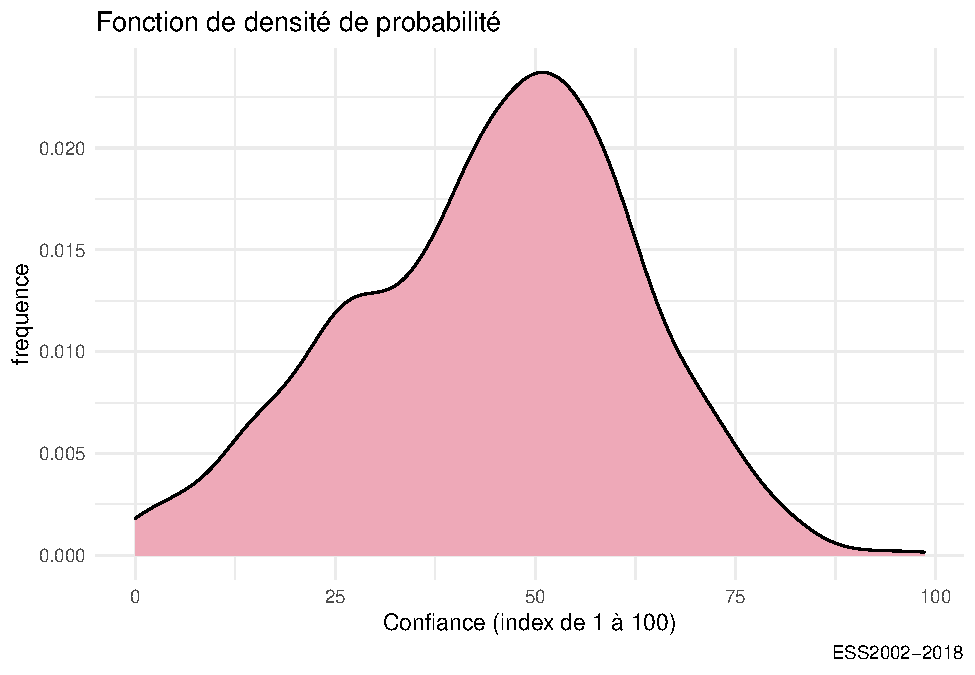
\includegraphics{bookdown-demo_files/figure-latex/304-1.pdf}
Enfin on peut examiner par rapport à une distribution théorique, en l'occurrence une distribution gaussienne, ou normale, de paramètres égaux à la moyenne et la variance empirique de la distribution. C'est ce que \texttt{stat\_function} permet de réaliser.

L'ajustement est convenable même si on observe une déviation sur la droite. C'est pourquoi on calcule aussi la Kurtosis et le skewness de la distribution.

\begin{Shaded}
\begin{Highlighting}[]
\CommentTok{\#On a déjà calculé la moyenne : mean}
\CommentTok{\#il nous manque l\textquotesingle{}écart{-}type et }
\NormalTok{sd}\OtherTok{\textless{}{-}}\FunctionTok{sd}\NormalTok{(foo}\SpecialCharTok{$}\NormalTok{trust\_institut, }\AttributeTok{na.rm=}\ConstantTok{TRUE}\NormalTok{)}
\FunctionTok{library}\NormalTok{(moments)}
\NormalTok{sk}\OtherTok{\textless{}{-}}\FunctionTok{skewness}\NormalTok{(foo}\SpecialCharTok{$}\NormalTok{trust\_institut)}
\NormalTok{ks}\OtherTok{\textless{}{-}}\FunctionTok{kurtosis}\NormalTok{(foo}\SpecialCharTok{$}\NormalTok{trust\_institut)}


\NormalTok{g05}\OtherTok{\textless{}{-}}\FunctionTok{ggplot}\NormalTok{(foo,}\FunctionTok{aes}\NormalTok{(}\AttributeTok{x=}\NormalTok{trust\_institut))}\SpecialCharTok{+}   
  \FunctionTok{labs}\NormalTok{(}\AttributeTok{title=} \StringTok{"Distribution de la confiance institutionnelle"}\NormalTok{, }\AttributeTok{caption=}\StringTok{"ESS2002{-}2018"}\NormalTok{,}\AttributeTok{y=} \StringTok{"frequence"}\NormalTok{,}\AttributeTok{x=}\StringTok{"confiance (index de 0 à 100)"}\NormalTok{) }\SpecialCharTok{+}
  \FunctionTok{geom\_density}\NormalTok{(}\AttributeTok{fill=}\StringTok{"pink2"}\NormalTok{)}\SpecialCharTok{+}
  \FunctionTok{stat\_function}\NormalTok{(}\AttributeTok{fun =}\NormalTok{ dnorm,}\AttributeTok{color=}\StringTok{"red"}\NormalTok{,}\AttributeTok{size=}\FloatTok{1.2}\NormalTok{, }\AttributeTok{args =} \FunctionTok{list}\NormalTok{(}\AttributeTok{mean =}\NormalTok{moy, }\AttributeTok{sd=}\NormalTok{sd))}
   
\NormalTok{g05}
\end{Highlighting}
\end{Shaded}

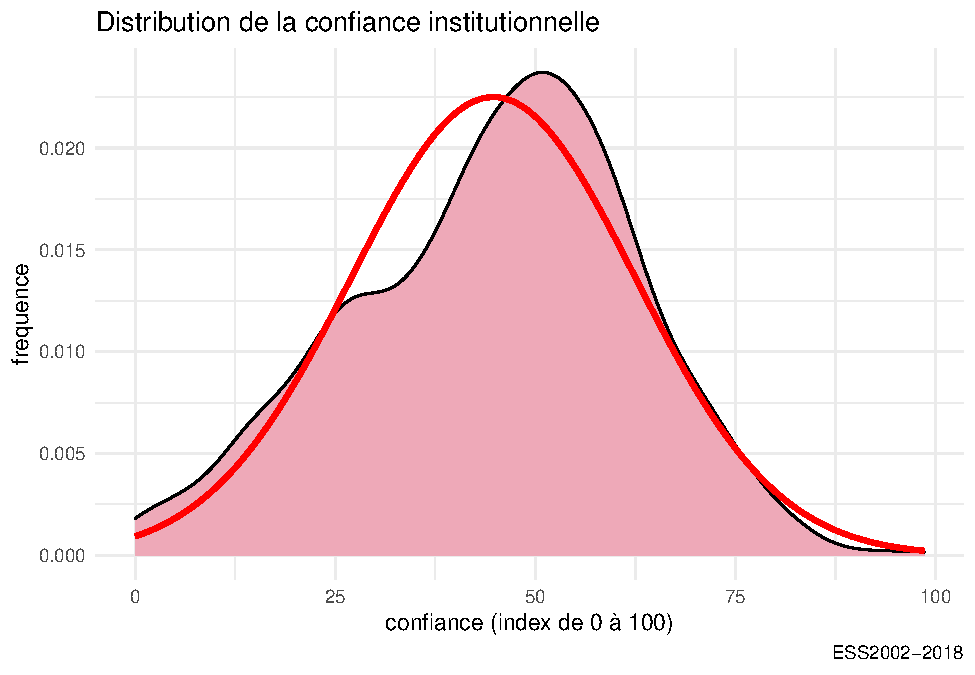
\includegraphics{bookdown-demo_files/figure-latex/305-1.pdf}

Un grand classique du test de normalité d'une distribution est le diagramme QQ.

\begin{Shaded}
\begin{Highlighting}[]
\NormalTok{g06 }\OtherTok{\textless{}{-}} \FunctionTok{ggplot}\NormalTok{(foo, }\FunctionTok{aes}\NormalTok{(}\AttributeTok{sample =}\NormalTok{ trust\_institut)) }\SpecialCharTok{+} 
  \FunctionTok{stat\_qq}\NormalTok{() }\SpecialCharTok{+} \FunctionTok{stat\_qq\_line}\NormalTok{()}\SpecialCharTok{+} 
  \FunctionTok{labs}\NormalTok{(}\AttributeTok{title=} \StringTok{"QQplot confiance interpersonnelle"}\NormalTok{, }
       \AttributeTok{caption=}\StringTok{"ESS2002{-}2018"}\NormalTok{,}
       \AttributeTok{y=} \StringTok{"Echantillon"}\NormalTok{,}\AttributeTok{x=}\StringTok{"Théorique"}\NormalTok{) }
\NormalTok{g06}
\end{Highlighting}
\end{Shaded}

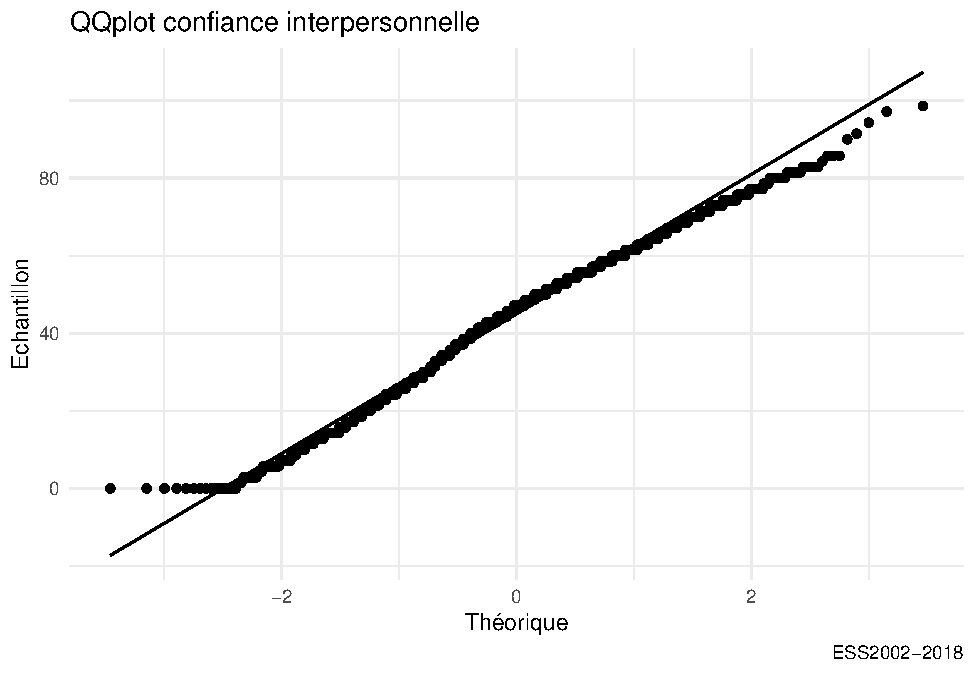
\includegraphics{bookdown-demo_files/figure-latex/306-1.pdf}

On finit cette étude détaillée par l'ajustement d'abord d'un modèle (loi normale) aux données. Ensuite d'un modèle de mélange ( Mixture model) par lequel on définit la loi de distribution sous-jascente, comme un mélange entre deux populations normale de paramètres distincts.

\url{https://tinyheero.github.io/2015/10/13/mixture-model.html}

\begin{Shaded}
\begin{Highlighting}[]
\NormalTok{df0}\OtherTok{\textless{}{-}}\NormalTok{df }\SpecialCharTok{\%\textgreater{}\%} 
  \FunctionTok{na.omit}\NormalTok{() }
\CommentTok{\#library(MASS)}
\NormalTok{fit}\OtherTok{\textless{}{-}}\FunctionTok{fitdistr}\NormalTok{(df0}\SpecialCharTok{$}\NormalTok{trust\_interpersonnel,}\StringTok{"normal"}\NormalTok{) }
\NormalTok{param}\OtherTok{\textless{}{-}}\FunctionTok{as.data.frame}\NormalTok{(fit}\SpecialCharTok{$}\NormalTok{estimate)}
\NormalTok{mean}\OtherTok{\textless{}{-}}\NormalTok{param[,}\DecValTok{1}\NormalTok{]}
\NormalTok{sd}\OtherTok{\textless{}{-}}\NormalTok{param[,}\DecValTok{1}\NormalTok{]}

\NormalTok{g07}\OtherTok{\textless{}{-}}\NormalTok{ g05}\SpecialCharTok{+}\FunctionTok{stat\_function}\NormalTok{(}\AttributeTok{fun =}\NormalTok{  dnorm ,}\AttributeTok{color=}\StringTok{"orange"}\NormalTok{,}\AttributeTok{size=}\FloatTok{1.2}\NormalTok{, }\AttributeTok{args =} \FunctionTok{list}\NormalTok{( }\AttributeTok{mean=}\NormalTok{mean,  }\AttributeTok{sd=}\NormalTok{sd))}
\NormalTok{g07}
\end{Highlighting}
\end{Shaded}

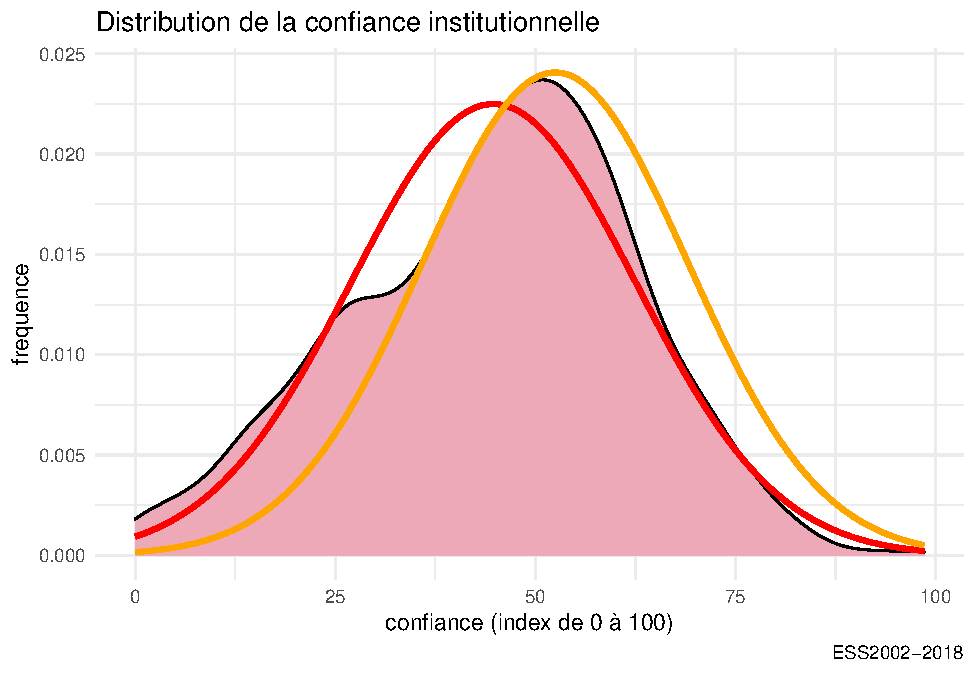
\includegraphics{bookdown-demo_files/figure-latex/307-1.pdf}

\begin{Shaded}
\begin{Highlighting}[]
\FunctionTok{library}\NormalTok{(mixtools)}
\NormalTok{trust }\OtherTok{=}\NormalTok{ foo}\SpecialCharTok{$}\NormalTok{trust\_institut}
\NormalTok{mixmdl }\OtherTok{=} \FunctionTok{normalmixEM}\NormalTok{(trust, }\AttributeTok{k=}\DecValTok{2}\NormalTok{)}
\end{Highlighting}
\end{Shaded}

\begin{verbatim}
## number of iterations= 237
\end{verbatim}

\begin{Shaded}
\begin{Highlighting}[]
\NormalTok{mixmdl}\SpecialCharTok{$}\NormalTok{mu}
\end{Highlighting}
\end{Shaded}

\begin{verbatim}
## [1] 20.77247 50.86798
\end{verbatim}

\begin{Shaded}
\begin{Highlighting}[]
\NormalTok{mixmdl}\SpecialCharTok{$}\NormalTok{sigma}
\end{Highlighting}
\end{Shaded}

\begin{verbatim}
## [1] 10.37739 13.51802
\end{verbatim}

\begin{Shaded}
\begin{Highlighting}[]
\NormalTok{mixmdl}\SpecialCharTok{$}\NormalTok{lambda}
\end{Highlighting}
\end{Shaded}

\begin{verbatim}
## [1] 0.2034332 0.7965668
\end{verbatim}

\begin{Shaded}
\begin{Highlighting}[]
\FunctionTok{plot}\NormalTok{(mixmdl,}\AttributeTok{which=}\DecValTok{2}\NormalTok{)}
\FunctionTok{lines}\NormalTok{(}\FunctionTok{density}\NormalTok{(trust), }\AttributeTok{lty=}\DecValTok{2}\NormalTok{, }\AttributeTok{lwd=}\DecValTok{2}\NormalTok{)}
\end{Highlighting}
\end{Shaded}

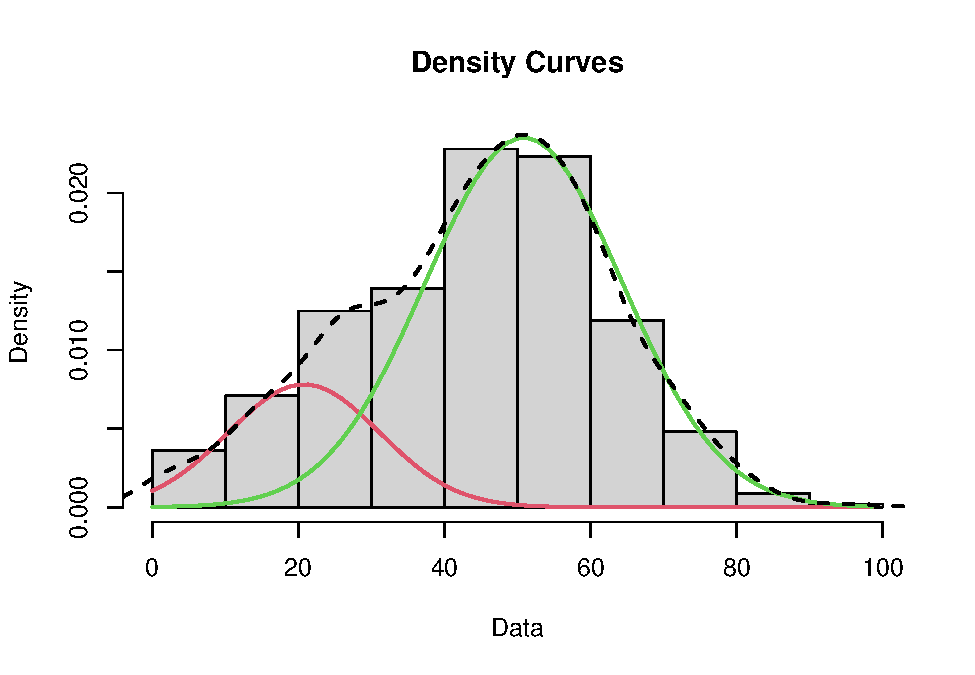
\includegraphics{bookdown-demo_files/figure-latex/307-2.pdf}

Finalement si notre distribution est univariée, car n'étudiant qu'une variable, on peut quand distinguer deux population distinctes.

\hypertarget{dautres-muxe9thodes}{%
\subsection{D'autres méthodes}\label{dautres-muxe9thodes}}

Il n'y a pas que l'histogramme ou le diagramme de densité, d'autres méthodes sont utiles, surtout quand on veut comparer des groupes (ce sera l'objet du prochain chapitre). Il s'agit du diagramme à moustache et du diagramme en violon.

\begin{Shaded}
\begin{Highlighting}[]
\NormalTok{g0306 }\OtherTok{\textless{}{-}} \FunctionTok{ggplot}\NormalTok{(foo, }\FunctionTok{aes}\NormalTok{(}\AttributeTok{y =}\NormalTok{ trust\_institut, }\AttributeTok{x=}\DecValTok{1}\NormalTok{)) }\SpecialCharTok{+} 
\FunctionTok{geom\_boxplot}\NormalTok{(}\AttributeTok{fill=}\StringTok{"Grey"}\NormalTok{) }

\NormalTok{g0307 }\OtherTok{\textless{}{-}} \FunctionTok{ggplot}\NormalTok{(foo, }\FunctionTok{aes}\NormalTok{(}\AttributeTok{x=}\DecValTok{1}\NormalTok{,}\AttributeTok{y =}\NormalTok{ trust\_institut)) }\SpecialCharTok{+} 
\FunctionTok{geom\_violin}\NormalTok{(}\AttributeTok{fill=}\StringTok{"Gold"}\NormalTok{) }\SpecialCharTok{+} \FunctionTok{labs}\NormalTok{(}\AttributeTok{x=}\StringTok{"density"}\NormalTok{)}

\FunctionTok{plot\_grid}\NormalTok{(g0306, g0307, }\AttributeTok{labels =} \FunctionTok{c}\NormalTok{(}\StringTok{"Boxplot"}\NormalTok{,}\StringTok{"Violin plot"}\NormalTok{),}
  \AttributeTok{label\_size =} \DecValTok{12}
\NormalTok{)}
\end{Highlighting}
\end{Shaded}

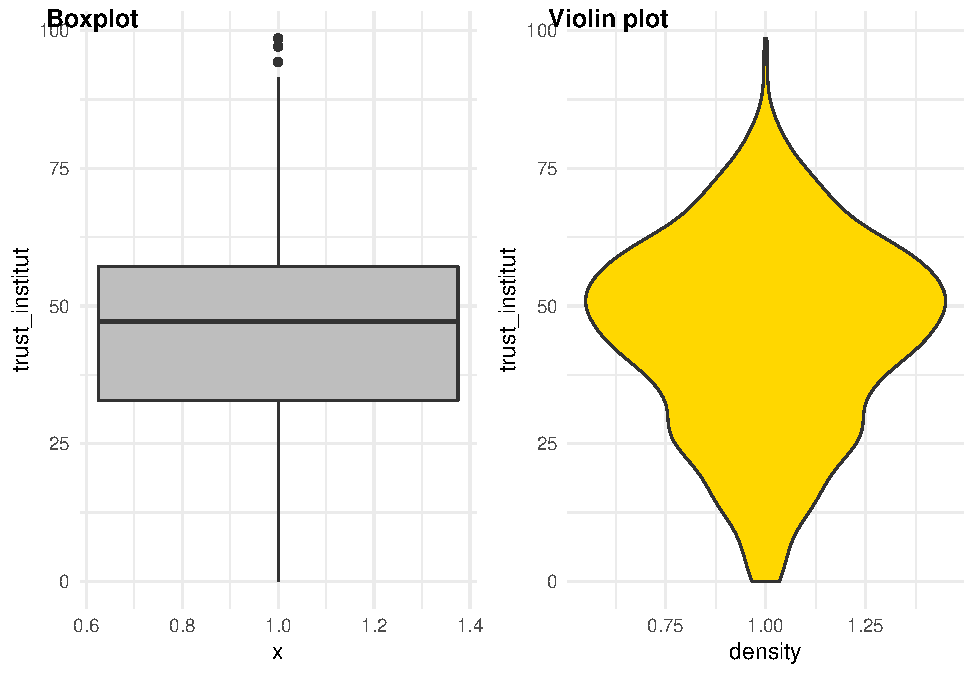
\includegraphics{bookdown-demo_files/figure-latex/308a-1.pdf}

\hypertarget{quand-la-variable-est-qualitative}{%
\subsection{Quand la variable est qualitative}\label{quand-la-variable-est-qualitative}}

Quand la variable est qualitative, que ses modalités sont discrètes, la manière de représenter la plus commune est le fameux \emph{camembert} que les experts abhorrent, n diagramme en barre représente mieux les proportions.

\begin{Shaded}
\begin{Highlighting}[]
\NormalTok{g08}\OtherTok{\textless{}{-}}\FunctionTok{ggplot}\NormalTok{(df,}\FunctionTok{aes}\NormalTok{(}\AttributeTok{x=}\NormalTok{age))}\SpecialCharTok{+}
  \FunctionTok{geom\_bar}\NormalTok{(}\AttributeTok{fill=}\StringTok{"skyblue"}\NormalTok{)}\SpecialCharTok{+}
  \FunctionTok{labs}\NormalTok{(}\AttributeTok{title=} \StringTok{"Distribution par classe d\textquotesingle{}âge"}\NormalTok{, }
       \AttributeTok{caption=}\StringTok{"ESS2002{-}2018"}\NormalTok{,}
       \AttributeTok{y=} \StringTok{"fréquence"}\NormalTok{,}
       \AttributeTok{x=}\StringTok{"Classes d\textquotesingle{}âge"}\NormalTok{) }
\NormalTok{g08}
\end{Highlighting}
\end{Shaded}

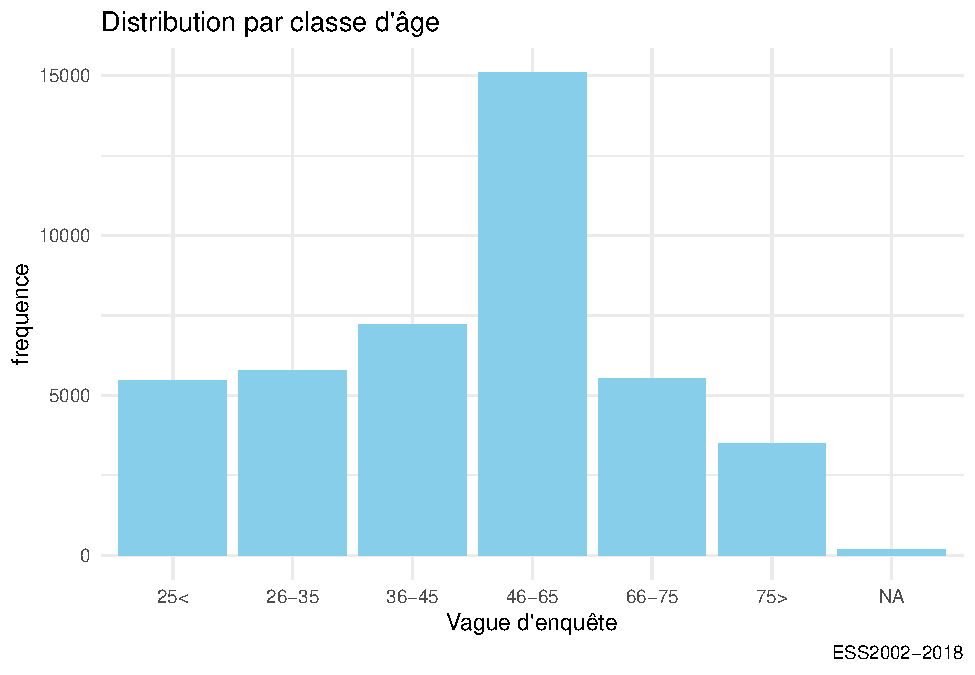
\includegraphics{bookdown-demo_files/figure-latex/308-1.pdf}

Avec quelques améliorations : contrôle de la couleurs des barres, ajout des \% et pivot pour une meilleure lecture.

\begin{Shaded}
\begin{Highlighting}[]
\NormalTok{foo}\OtherTok{\textless{}{-}}\NormalTok{df }\SpecialCharTok{\%\textgreater{}\%}
  \FunctionTok{filter}\NormalTok{(}\SpecialCharTok{!}\FunctionTok{is.na}\NormalTok{(age))}

\NormalTok{g10}\OtherTok{\textless{}{-}}\FunctionTok{ggplot}\NormalTok{(foo,}\FunctionTok{aes}\NormalTok{(}\AttributeTok{x=}\NormalTok{age, }\AttributeTok{y =} \FunctionTok{prop.table}\NormalTok{(}\FunctionTok{stat}\NormalTok{(count)),}\AttributeTok{label =}\NormalTok{ scales}\SpecialCharTok{::}\FunctionTok{percent}\NormalTok{(}\FunctionTok{prop.table}\NormalTok{(}\FunctionTok{stat}\NormalTok{(count)))))}\SpecialCharTok{+}
  \FunctionTok{geom\_bar}\NormalTok{(}\FunctionTok{aes}\NormalTok{(}\AttributeTok{fill =}\NormalTok{ age)) }\SpecialCharTok{+}  
  \FunctionTok{coord\_flip}\NormalTok{()}\SpecialCharTok{+} 
  \FunctionTok{labs}\NormalTok{(}\AttributeTok{title=} \StringTok{"Répartition de la population par classe d\textquotesingle{}âge"}\NormalTok{, }\AttributeTok{caption=}\StringTok{"ESS2002{-}2018"}\NormalTok{,}\AttributeTok{y=} \StringTok{"\%"}\NormalTok{,}\AttributeTok{x=}\StringTok{"classes d\textquotesingle{}age"}\NormalTok{) }\SpecialCharTok{+}
  \FunctionTok{scale\_y\_continuous}\NormalTok{(}\AttributeTok{labels =}\NormalTok{ scales}\SpecialCharTok{::}\NormalTok{percent)}\SpecialCharTok{+} \CommentTok{\#contrôle de l\textquotesingle{}échelle des \% et du format}
  \FunctionTok{scale\_fill\_brewer}\NormalTok{()}\SpecialCharTok{+}
  \FunctionTok{geom\_text}\NormalTok{(}\AttributeTok{stat =} \StringTok{\textquotesingle{}count\textquotesingle{}}\NormalTok{,}\AttributeTok{position =} \FunctionTok{position\_dodge}\NormalTok{(.}\DecValTok{9}\NormalTok{),  }\AttributeTok{hjust =} \DecValTok{1}\NormalTok{, }\AttributeTok{size =} \DecValTok{3}\NormalTok{)}


\NormalTok{g10}
\end{Highlighting}
\end{Shaded}

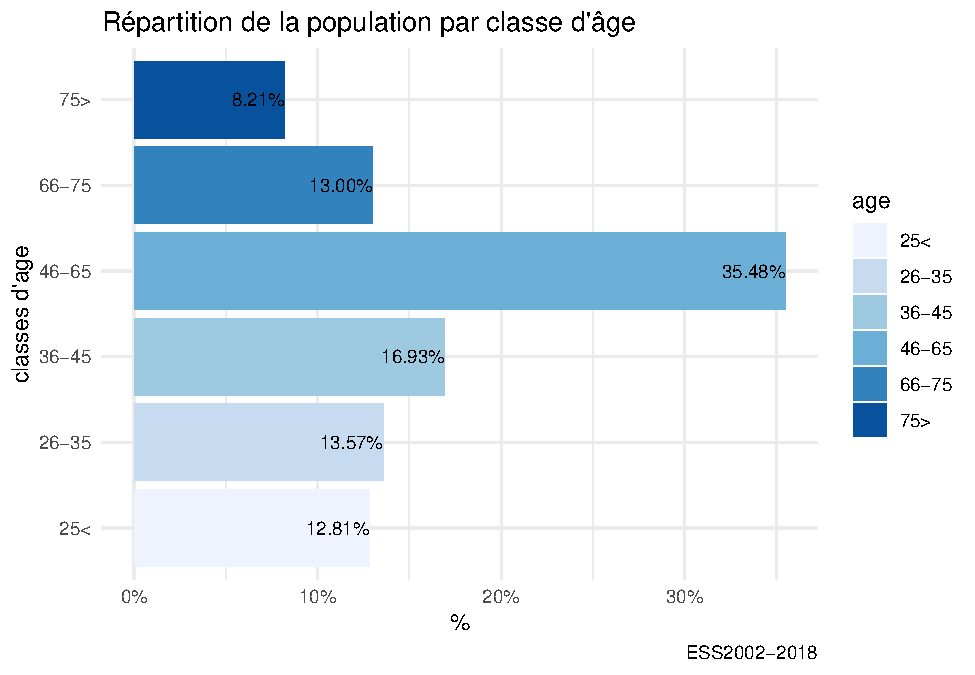
\includegraphics{bookdown-demo_files/figure-latex/309-1.pdf}

\begin{Shaded}
\begin{Highlighting}[]
\NormalTok{g11}\OtherTok{\textless{}{-}}\FunctionTok{ggplot}\NormalTok{(foo,}\FunctionTok{aes}\NormalTok{(}\AttributeTok{x=}\FunctionTok{factor}\NormalTok{(}\DecValTok{1}\NormalTok{),}\AttributeTok{fill=}\NormalTok{age, }\AttributeTok{y =} \FunctionTok{prop.table}\NormalTok{(}\FunctionTok{stat}\NormalTok{(count)),}\AttributeTok{label =}\NormalTok{scales}\SpecialCharTok{::}\FunctionTok{percent}\NormalTok{(}\FunctionTok{prop.table}\NormalTok{(}\FunctionTok{stat}\NormalTok{(count)))))}\SpecialCharTok{+}
  \FunctionTok{geom\_bar}\NormalTok{(}\AttributeTok{width=}\DecValTok{1}\NormalTok{) }\SpecialCharTok{+}  
  \FunctionTok{coord\_flip}\NormalTok{()}\SpecialCharTok{+} 
  \FunctionTok{labs}\NormalTok{(}\AttributeTok{title=} \StringTok{"Répartition de la population par classe d\textquotesingle{}âge"}\NormalTok{, }\AttributeTok{caption=}\StringTok{"ESS2002{-}2018"}\NormalTok{,}\AttributeTok{y=} \StringTok{"\%"}\NormalTok{,}\AttributeTok{x=}\StringTok{"classes d\textquotesingle{}age"}\NormalTok{) }\SpecialCharTok{+}
  \FunctionTok{geom\_text}\NormalTok{(}\AttributeTok{stat =} \StringTok{\textquotesingle{}count\textquotesingle{}}\NormalTok{,}\AttributeTok{position =} \FunctionTok{position\_dodge}\NormalTok{(.}\DecValTok{9}\NormalTok{),  }\AttributeTok{hjust =} \DecValTok{1}\NormalTok{, }\AttributeTok{size =} \DecValTok{3}\NormalTok{)}

\NormalTok{g11}
\end{Highlighting}
\end{Shaded}

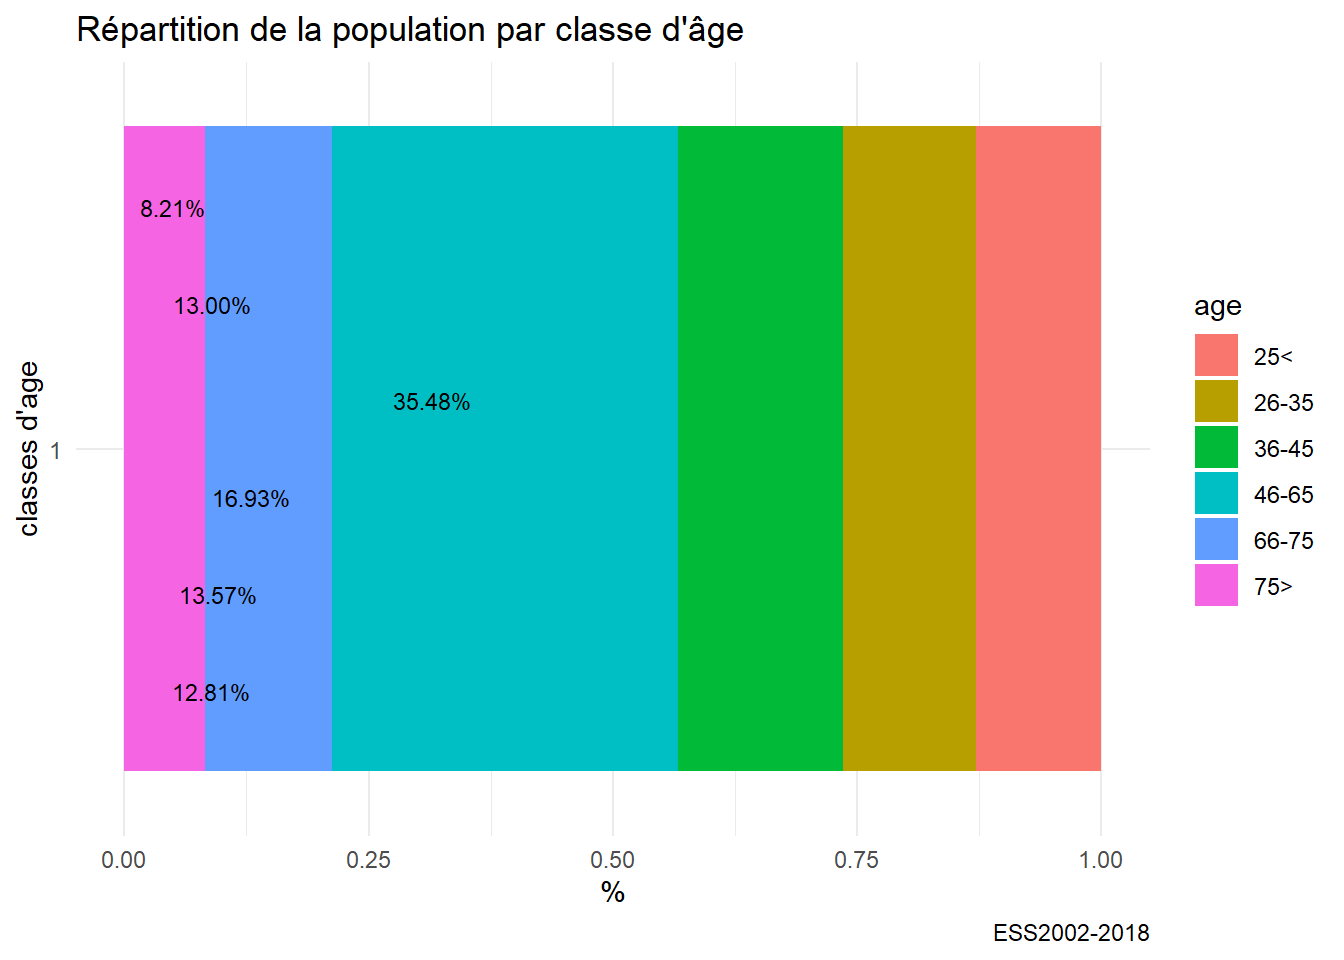
\includegraphics{bookdown-demo_files/figure-latex/309-2.pdf}

si on tient au diagramme en secteur

\begin{Shaded}
\begin{Highlighting}[]
\NormalTok{foo}\OtherTok{\textless{}{-}}\NormalTok{df }\SpecialCharTok{\%\textgreater{}\%}\FunctionTok{filter}\NormalTok{(}\SpecialCharTok{!}\FunctionTok{is.na}\NormalTok{(age))}
\NormalTok{g10}\OtherTok{\textless{}{-}}\FunctionTok{ggplot}\NormalTok{(foo,}\FunctionTok{aes}\NormalTok{(}\AttributeTok{x=}\StringTok{""}\NormalTok{, }\AttributeTok{y =} \FunctionTok{prop.table}\NormalTok{(}\FunctionTok{stat}\NormalTok{(count)),}
                    \AttributeTok{label =}\NormalTok{ scales}\SpecialCharTok{::}\FunctionTok{percent}\NormalTok{(}\FunctionTok{prop.table}\NormalTok{(}\FunctionTok{stat}\NormalTok{(count)))))}\SpecialCharTok{+}
  \FunctionTok{geom\_bar}\NormalTok{(}\FunctionTok{aes}\NormalTok{(}\AttributeTok{fill =}\NormalTok{ age)) }\SpecialCharTok{+}  
  \FunctionTok{labs}\NormalTok{(}\AttributeTok{title=} \StringTok{"Répartition de la population par classe d\textquotesingle{}âge"}\NormalTok{, }
       \AttributeTok{caption=}\StringTok{"ESS2002{-}2018"}\NormalTok{,}\AttributeTok{y=} \StringTok{"\%"}\NormalTok{,}\AttributeTok{x=}\StringTok{"classes d\textquotesingle{}age"}\NormalTok{) }\SpecialCharTok{+}
  \FunctionTok{geom\_text}\NormalTok{(}\AttributeTok{stat =} \StringTok{\textquotesingle{}count\textquotesingle{}}\NormalTok{,}\AttributeTok{position =} \FunctionTok{position\_dodge}\NormalTok{(.}\DecValTok{9}\NormalTok{),  }\AttributeTok{hjust =} \DecValTok{1}\NormalTok{, }\AttributeTok{size =} \DecValTok{3}\NormalTok{) }\SpecialCharTok{+} 
  \FunctionTok{coord\_polar}\NormalTok{(}\StringTok{"y"}\NormalTok{, }\AttributeTok{start=}\DecValTok{0}\NormalTok{)}

\NormalTok{g10}
\end{Highlighting}
\end{Shaded}

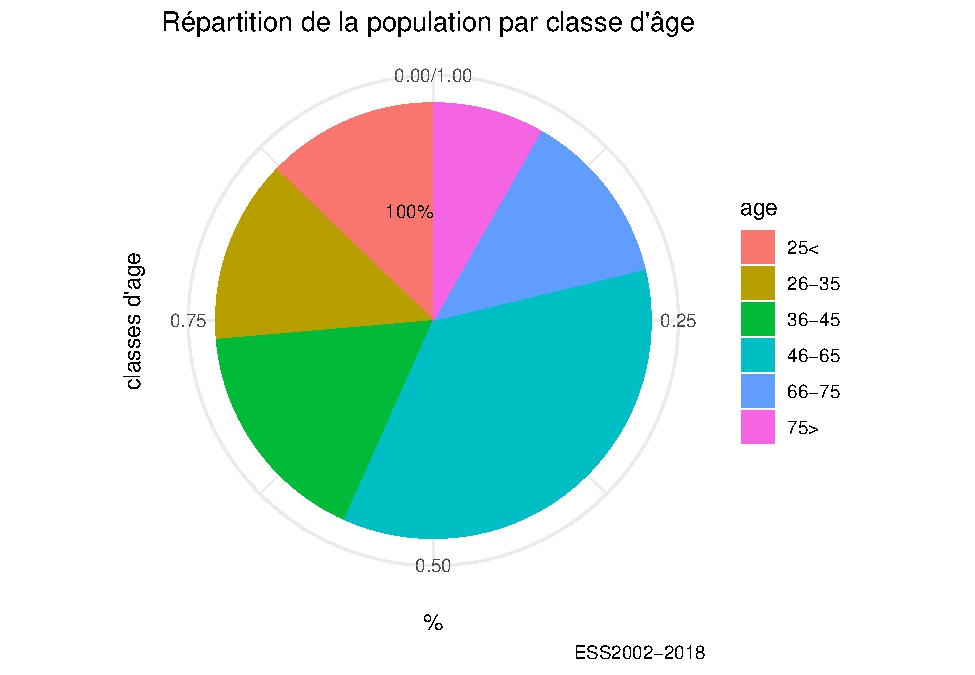
\includegraphics{bookdown-demo_files/figure-latex/310-1.pdf}
\url{https://cran.r-project.org/web/packages/treemapify/vignettes/introduction-to-treemapify.html}

si on tient au diagramme en cercle, autant opter pour un treemap avec la bibliothèque treemapifi

\begin{Shaded}
\begin{Highlighting}[]
\FunctionTok{library}\NormalTok{(treemapify)}
\NormalTok{tree1}\OtherTok{\textless{}{-}}\NormalTok{df }\SpecialCharTok{\%\textgreater{}\%} 
  \FunctionTok{mutate}\NormalTok{(}\AttributeTok{n=}\DecValTok{1}\NormalTok{)}\SpecialCharTok{\%\textgreater{}\%}\FunctionTok{group\_by}\NormalTok{(age) }\SpecialCharTok{\%\textgreater{}\%} 
  \FunctionTok{summarize}\NormalTok{(}\AttributeTok{n=}\FunctionTok{sum}\NormalTok{(n)) }\SpecialCharTok{\%\textgreater{}\%}
  \FunctionTok{filter}\NormalTok{(}\SpecialCharTok{!}\FunctionTok{is.na}\NormalTok{(age))}

\NormalTok{g11 }\OtherTok{\textless{}{-}} \FunctionTok{ggplot}\NormalTok{(tree1, }\FunctionTok{aes}\NormalTok{(}\AttributeTok{area =}\NormalTok{ n, }\AttributeTok{fill=}\NormalTok{n),}\AttributeTok{label=}\NormalTok{age) }\SpecialCharTok{+}
  \FunctionTok{geom\_treemap}\NormalTok{() }\SpecialCharTok{+}
  \FunctionTok{geom\_treemap\_text}\NormalTok{(}\FunctionTok{aes}\NormalTok{(}\AttributeTok{label=}\NormalTok{age),}\AttributeTok{colour =} \StringTok{"white"}\NormalTok{, }\AttributeTok{place =} \StringTok{"centre"}\NormalTok{,}\AttributeTok{grow =} \ConstantTok{FALSE}\NormalTok{)}\SpecialCharTok{+}
  \FunctionTok{labs}\NormalTok{(}\AttributeTok{title=} \StringTok{"Répartition de la population par classe d\textquotesingle{}âge"}\NormalTok{, }\AttributeTok{caption=}\StringTok{"ESS2002{-}2018"}\NormalTok{,}\AttributeTok{y=} \ConstantTok{NULL}\NormalTok{,}\AttributeTok{x=}\ConstantTok{NULL}\NormalTok{) }

\NormalTok{g11}
\end{Highlighting}
\end{Shaded}

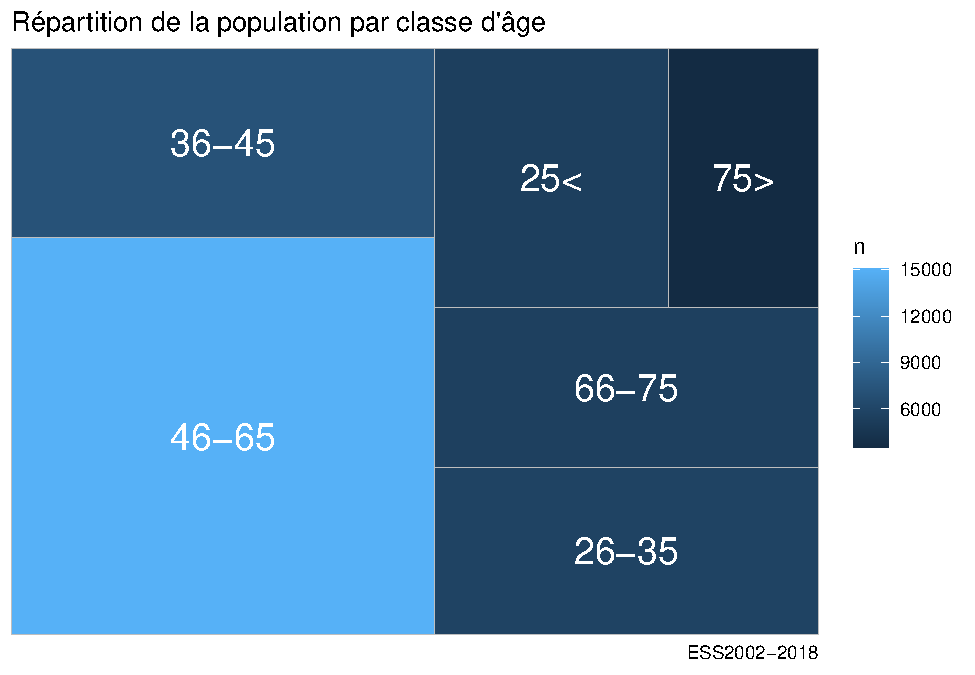
\includegraphics{bookdown-demo_files/figure-latex/311-1.pdf}

\hypertarget{analyse-bi-variuxe9e}{%
\chapter{Analyse bi variée}\label{analyse-bi-variuxe9e}}

Comme son nom l'indique, il s'agit d'examiner la relation entre deux variables et d'étudier leur distribution conjointe. On distinguera 3 situations et on examinera pour chaune les modes de représentations graphiques ainsi que les tests associés qui permette de s'assurer que la relation apparente est effective.

\begin{enumerate}
\def\labelenumi{\alph{enumi})}
\item
  Deux variables quantitatives : scatterplot et corélations
\item
  deux variable qualitatives : tableau croisé et test du chi2
\item
  une variable quanti et une variable quali. Compariaons de moyennes et ANOVA
\item
  par comparer des distribution de plusieurs groupes (variables catégorielles)
\item
  par comparer des moyennes d'une variable dépendante en fonction de plusieurs variables indépendantes catégorielle
\item
  mesurer l'association entre deux variables qualitatives
\end{enumerate}

\hypertarget{diagrammes-xy---la-magie-des-corruxe9lations}{%
\section{Diagrammes xy - la magie des corrélations}\label{diagrammes-xy---la-magie-des-corruxe9lations}}

Venons en à analyser les relations entre deux variables quantitatives.

\begin{Shaded}
\begin{Highlighting}[]
\NormalTok{foo}\OtherTok{\textless{}{-}}\NormalTok{df }\SpecialCharTok{\%\textgreater{}\%}
  \FunctionTok{filter}\NormalTok{(cntry}\SpecialCharTok{==}\StringTok{"FR"} \SpecialCharTok{\&}\NormalTok{ Year}\SpecialCharTok{==}\StringTok{"2018"}\NormalTok{) }\CommentTok{\#selection de l\textquotesingle{}echantillon}

\NormalTok{g31}\OtherTok{\textless{}{-}} \FunctionTok{ggplot}\NormalTok{(foo, }\FunctionTok{aes}\NormalTok{(}\AttributeTok{x=}\NormalTok{ trust\_interpersonnel,}\AttributeTok{y=}\NormalTok{trust\_institut)) }\SpecialCharTok{+}
  \FunctionTok{geom\_point}\NormalTok{( }\AttributeTok{size=}\FloatTok{0.1}\NormalTok{)}
     
\NormalTok{g31}
\end{Highlighting}
\end{Shaded}

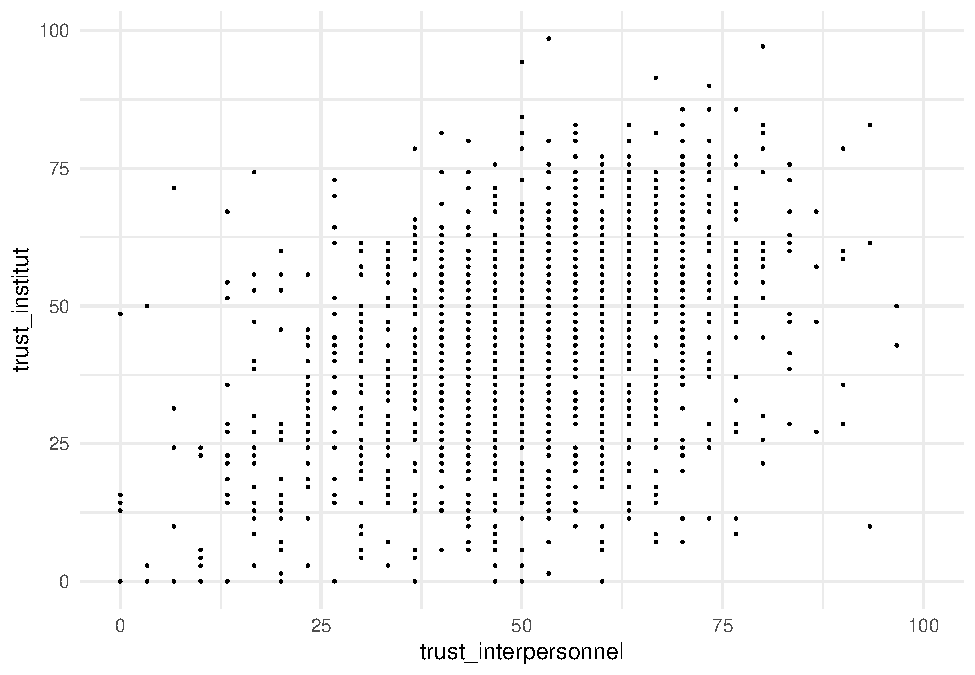
\includegraphics{bookdown-demo_files/figure-latex/412-1.pdf}

Ce graphe est peu clair, il y a trop de points qui prennent des valeurs discrètes. Une astuce est de donner une position aléatoire pour sur disperser, on fait mieux apparaitre la densité de points. On ajoute la représentation de deux courbe d'ajustement, l'une linéraire et l'autre non linéaires.

Mais en attendant en voici un calcul élémentaire.

le calcul de la variance

\[{SS}_{xx} = \sum (x - \bar{x})^2 = \sum x^2 - \frac {(\sum x)^2}{n}\]
le calcul de la covariance

\[{SS}_{xy} = \sum (x - \bar{x})(y - \bar{y}) = \sum xy - \frac {(\sum x)(\sum y)}{n}\]
et la corrélation qui est le rapport de la covariance sur la racine carrée du produit des variances de x et y.

\[r = \frac {{SS}_{xy}}{\sqrt {{SS}_{xx}{SS}_{yy}}}\]

La corrélation est de l'ordre d'un peu plus de 0,40 ce qui est assez élevé mais laisse une certaine indépendance des variables. Elle désignent des objets liés mais distinct. On peut tester l'hypothèse qu'en réalité cette corrélation est nulle. Le test conduit au rejet de l'hypothèse nulle de manière très nette, compte-tenu de l'échantillon l'intervalle de confiance est compris entre 0.36 et 0.44.

\begin{Shaded}
\begin{Highlighting}[]
\CommentTok{\#psych}
\NormalTok{r}\OtherTok{\textless{}{-}}\FunctionTok{cor.test}\NormalTok{(foo}\SpecialCharTok{$}\NormalTok{trust\_interpersonnel, foo}\SpecialCharTok{$}\NormalTok{trust\_institut) }\CommentTok{\#le test vient du package psych}
\NormalTok{r}
\end{Highlighting}
\end{Shaded}

\begin{verbatim}
## 
##  Pearson's product-moment correlation
## 
## data:  foo$trust_interpersonnel and foo$trust_institut
## t = 18.861, df = 1821, p-value < 2.2e-16
## alternative hypothesis: true correlation is not equal to 0
## 95 percent confidence interval:
##  0.3651235 0.4419644
## sample estimates:
##      cor 
## 0.404257
\end{verbatim}

\begin{Shaded}
\begin{Highlighting}[]
\NormalTok{rp}\OtherTok{\textless{}{-}}\FunctionTok{round}\NormalTok{(r}\SpecialCharTok{$}\NormalTok{estimate,}\DecValTok{3}\NormalTok{)}
\NormalTok{rp}
\end{Highlighting}
\end{Shaded}

\begin{verbatim}
##   cor 
## 0.404
\end{verbatim}

Améliorons le graphe On peut souhaiter ajouter une droite des moindre carrés (calculée pour chaque vague d'enquête pour évaluer la stabilité de la relation dans le temps). Les lignes sont parallèles, la corrélation ne change pas dans le temps, c'est une relation stable. Les deux formes de confiance vont dans le meme sens. On verra dans un autre chapitre comment calculer ces droites de corrélations.

\begin{Shaded}
\begin{Highlighting}[]
\FunctionTok{library}\NormalTok{(ggExtra)}
\NormalTok{g32}\OtherTok{\textless{}{-}}\FunctionTok{ggplot}\NormalTok{(foo, }\FunctionTok{aes}\NormalTok{(}\AttributeTok{x=}\NormalTok{ trust\_interpersonnel,}\AttributeTok{y=}\NormalTok{trust\_institut)) }\SpecialCharTok{+}
  \FunctionTok{geom\_point}\NormalTok{(}\AttributeTok{position =} \StringTok{"jitter"}\NormalTok{, }\AttributeTok{size=}\FloatTok{0.1}\NormalTok{, }\AttributeTok{color=}\StringTok{"grey"}\NormalTok{)}\SpecialCharTok{+}
  \FunctionTok{geom\_smooth}\NormalTok{(}\AttributeTok{method=}\StringTok{"lm"}\NormalTok{, }\AttributeTok{se=}\ConstantTok{TRUE}\NormalTok{) }\SpecialCharTok{+}
  \FunctionTok{geom\_smooth}\NormalTok{(}\AttributeTok{method=}\StringTok{"gam"}\NormalTok{,}\AttributeTok{color=}\StringTok{"red"}\NormalTok{)     }\SpecialCharTok{+}
  \FunctionTok{labs}\NormalTok{(}\AttributeTok{title =} \StringTok{"Relation entre confiance }\SpecialCharTok{\textbackslash{}n}\StringTok{institutionnelle et interpersonnelle"}\NormalTok{, }
       \AttributeTok{subtitle =} \FunctionTok{paste}\NormalTok{(}\StringTok{"r de pearson: "}\NormalTok{,rp ),}
       \AttributeTok{x=} \StringTok{"Confiance interpersonnelle"}\NormalTok{,}
       \AttributeTok{y=}\StringTok{" Confiance institutionnelle"}\NormalTok{)}

\FunctionTok{ggMarginal}\NormalTok{(g32  ,}\AttributeTok{type =} \StringTok{"density"}\NormalTok{, }\AttributeTok{fill =} \StringTok{"Royalblue1"}\NormalTok{, }\AttributeTok{alpha=}\NormalTok{.}\DecValTok{5}\NormalTok{)}
\end{Highlighting}
\end{Shaded}

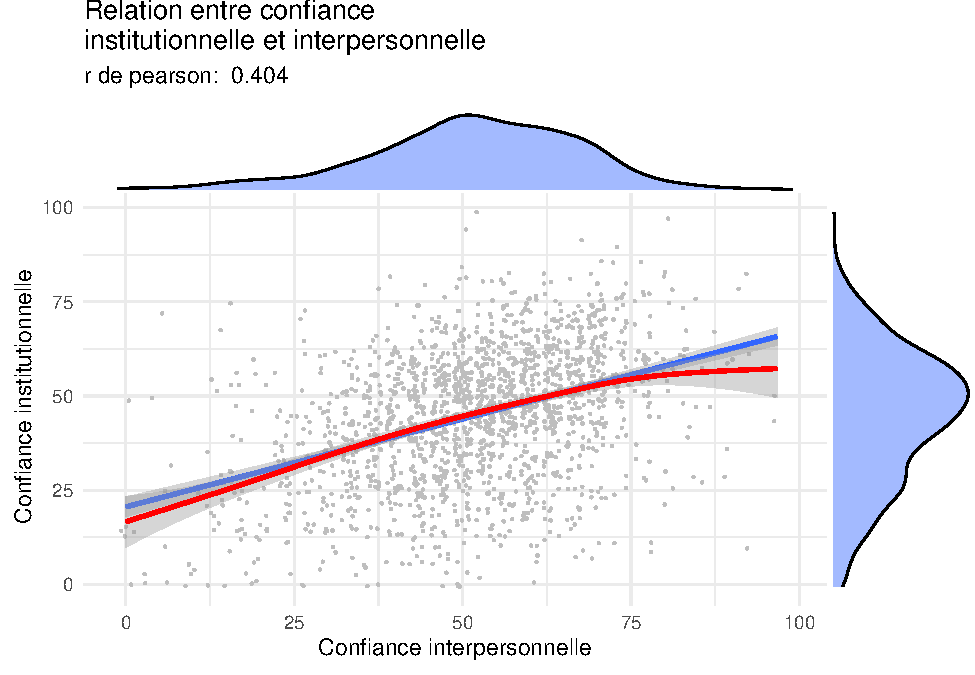
\includegraphics{bookdown-demo_files/figure-latex/0415-1.pdf}
Une autre façon de représenter est celle de carte de densité de probabilité.

\begin{Shaded}
\begin{Highlighting}[]
\NormalTok{g32}\OtherTok{\textless{}{-}}\FunctionTok{ggplot}\NormalTok{(foo, }\FunctionTok{aes}\NormalTok{(}\AttributeTok{x=}\NormalTok{ trust\_interpersonnel,}\AttributeTok{y=}\NormalTok{trust\_institut)) }\SpecialCharTok{+}
  \FunctionTok{geom\_point}\NormalTok{(}\AttributeTok{position =} \StringTok{"jitter"}\NormalTok{, }\AttributeTok{size=}\FloatTok{0.1}\NormalTok{, }\AttributeTok{color=}\StringTok{"grey"}\NormalTok{)}\SpecialCharTok{+}\FunctionTok{geom\_density2d}\NormalTok{()}\SpecialCharTok{+}
  \FunctionTok{labs}\NormalTok{(}\AttributeTok{title =} \StringTok{"Relation entre confiance institutionnelle et interpersonnelles"}\NormalTok{, }\AttributeTok{subtitle =} \FunctionTok{paste}\NormalTok{(}\StringTok{"r de pearson: "}\NormalTok{,rp ))}
  
\NormalTok{g33}\OtherTok{\textless{}{-}}\FunctionTok{ggplot}\NormalTok{(foo, }\FunctionTok{aes}\NormalTok{(}\AttributeTok{x=}\NormalTok{ trust\_interpersonnel,}\AttributeTok{y=}\NormalTok{trust\_institut)) }\SpecialCharTok{+}
  \FunctionTok{geom\_density2d\_filled}\NormalTok{(}\FunctionTok{aes}\NormalTok{(}\AttributeTok{fill =}\NormalTok{ ..level.., }\AttributeTok{color =}\NormalTok{ ..level..),}
    \AttributeTok{contour\_var =} \StringTok{"density"}\NormalTok{)}\SpecialCharTok{+}
  \FunctionTok{labs}\NormalTok{(}\AttributeTok{title =} \StringTok{"Relation entre confiance institutionnelle et interpersonnelles"}\NormalTok{, }\AttributeTok{subtitle =} \FunctionTok{paste}\NormalTok{(}\StringTok{"r de pearson: "}\NormalTok{,rp ))}\SpecialCharTok{+}\FunctionTok{theme}\NormalTok{(}\AttributeTok{legend.position =} \StringTok{"none"}\NormalTok{)}
  

\FunctionTok{plot\_grid}\NormalTok{(g32, g33, }\AttributeTok{labels =} \FunctionTok{c}\NormalTok{(}\StringTok{\textquotesingle{}A\textquotesingle{}}\NormalTok{, }\StringTok{\textquotesingle{}B\textquotesingle{}}\NormalTok{), }\AttributeTok{label\_size =} \DecValTok{12}\NormalTok{)}
\end{Highlighting}
\end{Shaded}

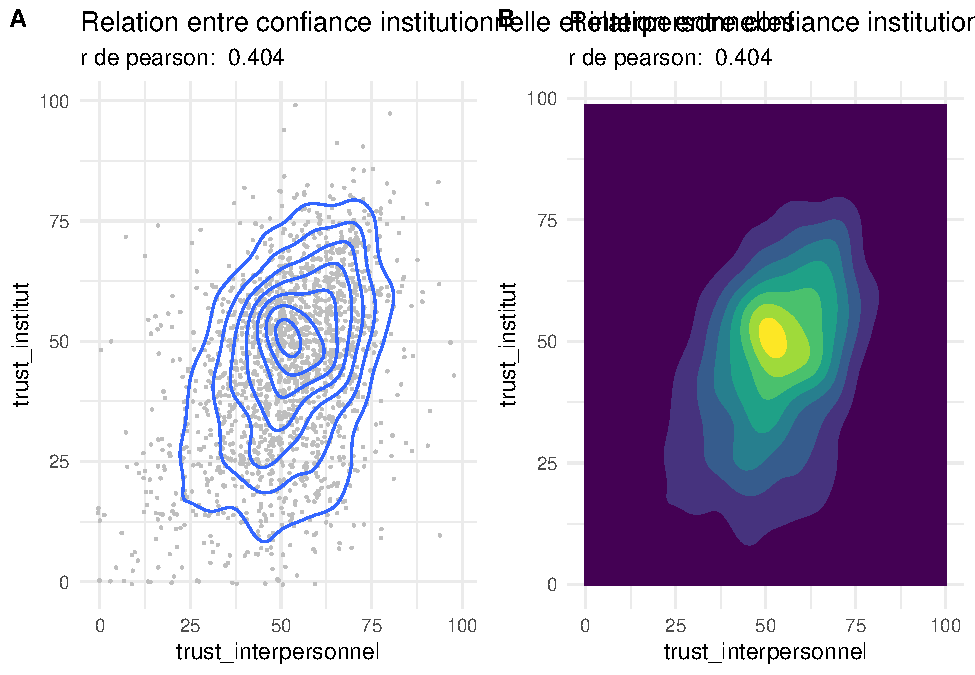
\includegraphics{bookdown-demo_files/figure-latex/416-1.pdf}

\hypertarget{comparer-les-distributions-et-des-moyennes}{%
\section{Comparer les distributions et des moyennes}\label{comparer-les-distributions-et-des-moyennes}}

Dans notre base on a pris les données de l'Allemagne et de la France. On va comparer leur distribution. Et tant qu'à faire, puisque qu'on a deux variables, on va faire deux comparaisons : par pays et par type de confiance.

A cette fin, nous construisons un tableau de données spécifique.

\begin{Shaded}
\begin{Highlighting}[]
\CommentTok{\#on recode en facteur la variable}

\NormalTok{foo }\OtherTok{\textless{}{-}}\NormalTok{ df }\SpecialCharTok{\%\textgreater{}\%} 
\NormalTok{  dplyr}\SpecialCharTok{::}\FunctionTok{select}\NormalTok{(cntry,trust\_institut, Year,trust\_interpersonnel) }\SpecialCharTok{\%\textgreater{}\%}
  \FunctionTok{filter}\NormalTok{( Year}\SpecialCharTok{==}\StringTok{"2018"}\NormalTok{) }\SpecialCharTok{\%\textgreater{}\%} 
\NormalTok{ dplyr}\SpecialCharTok{::}\FunctionTok{select}\NormalTok{(}\SpecialCharTok{{-}}\NormalTok{Year)}\SpecialCharTok{\%\textgreater{}\%}
 \FunctionTok{drop\_na}\NormalTok{() }\SpecialCharTok{\%\textgreater{}\%}
  \FunctionTok{gather}\NormalTok{(variable, value, }\SpecialCharTok{{-}}\NormalTok{cntry) }\CommentTok{\#attention plutôt utiliser pivot\_longer}

\FunctionTok{head}\NormalTok{(foo)}
\end{Highlighting}
\end{Shaded}

\begin{verbatim}
## # A tibble: 6 x 3
##   cntry        variable       value
##   <chr+lbl>    <chr>          <dbl>
## 1 DE [Germany] trust_institut  58.6
## 2 DE [Germany] trust_institut  65.7
## 3 DE [Germany] trust_institut  58.6
## 4 DE [Germany] trust_institut  65.7
## 5 DE [Germany] trust_institut  48.6
## 6 DE [Germany] trust_institut  37.1
\end{verbatim}

Pour la représentation, en plus de la représentation en terme de densité, on va choisir une méthode de violon et de boxplot. On utilise une couche de ``facetting'' pour éclater ainsi la distribution des deux variables selon un critère de pays.

\begin{Shaded}
\begin{Highlighting}[]
\CommentTok{\#on peut utiliser "facet"}
\NormalTok{g20}\OtherTok{\textless{}{-}}\FunctionTok{ggplot}\NormalTok{(foo,}\FunctionTok{aes}\NormalTok{(}\AttributeTok{x=}\NormalTok{value))}\SpecialCharTok{+} \FunctionTok{geom\_density}\NormalTok{(}\AttributeTok{binwidth=}\DecValTok{10}\NormalTok{, }\AttributeTok{fill=}\StringTok{"pink"}\NormalTok{)}\SpecialCharTok{+} \FunctionTok{facet\_grid}\NormalTok{(cntry}\SpecialCharTok{\textasciitilde{}}\NormalTok{variable)}\SpecialCharTok{+}   
  \FunctionTok{labs}\NormalTok{(}\AttributeTok{title=} \StringTok{"Confiance institutionnnelle"}\NormalTok{, }\AttributeTok{caption=}\StringTok{"ESS2002{-}2018"}\NormalTok{,}\AttributeTok{y=} \StringTok{"frequence"}\NormalTok{,}\AttributeTok{x=}\StringTok{"Confiance"}\NormalTok{)}
\NormalTok{g20}
\end{Highlighting}
\end{Shaded}

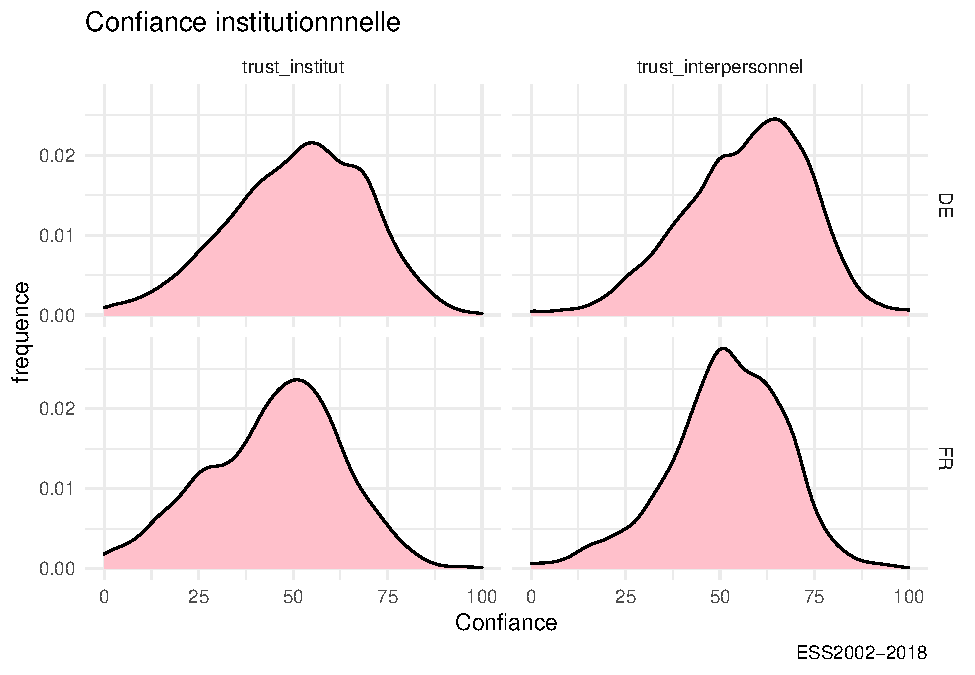
\includegraphics{bookdown-demo_files/figure-latex/418-1.pdf}

\begin{Shaded}
\begin{Highlighting}[]
\NormalTok{g21}\OtherTok{\textless{}{-}}\FunctionTok{ggplot}\NormalTok{(foo,}\FunctionTok{aes}\NormalTok{(}\AttributeTok{x=}\NormalTok{variable, }\AttributeTok{y=}\NormalTok{value))}\SpecialCharTok{+} 
  \FunctionTok{geom\_violin}\NormalTok{( }\AttributeTok{fill=}\StringTok{"pink"}\NormalTok{) }\SpecialCharTok{+} 
  \FunctionTok{geom\_boxplot}\NormalTok{(}\AttributeTok{width=}\FloatTok{0.1}\NormalTok{)}\SpecialCharTok{+}
  \FunctionTok{facet\_grid}\NormalTok{(cntry}\SpecialCharTok{\textasciitilde{}}\NormalTok{.)}\SpecialCharTok{+}   
  \FunctionTok{labs}\NormalTok{(}\AttributeTok{title=} \StringTok{"Confiance institutionnnelle"}\NormalTok{, }\AttributeTok{caption=}\StringTok{"ESS2002{-}2018"}\NormalTok{,}\AttributeTok{y=} \StringTok{"frequence"}\NormalTok{,}\AttributeTok{x=}\StringTok{"Confiance"}\NormalTok{)}
\NormalTok{g21}
\end{Highlighting}
\end{Shaded}

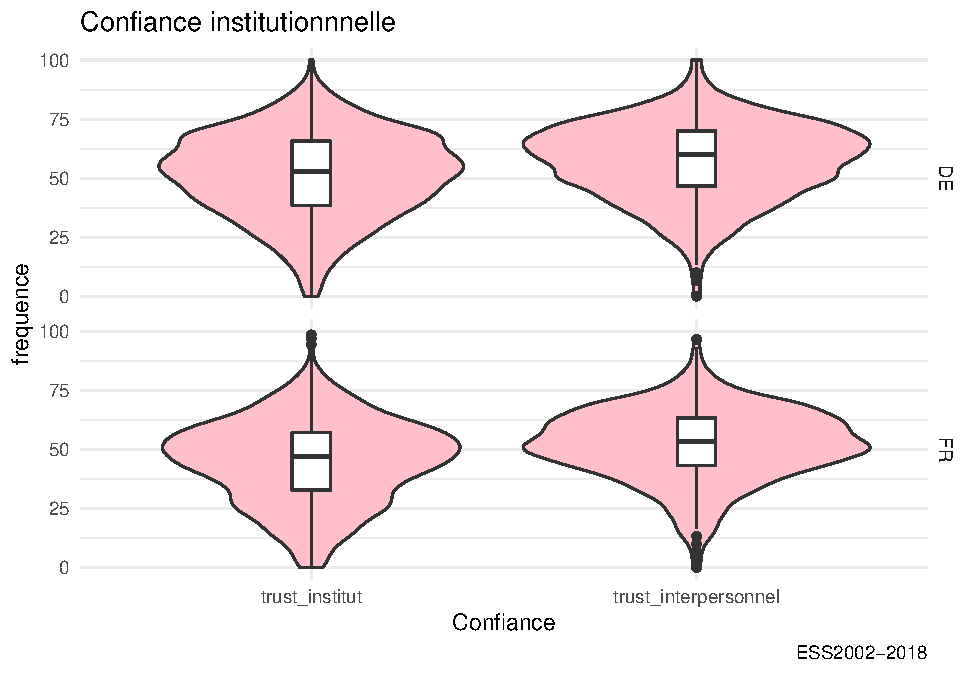
\includegraphics{bookdown-demo_files/figure-latex/418-2.pdf}

\hypertarget{comparaison-de-moyennes}{%
\subsection{Comparaison de moyennes}\label{comparaison-de-moyennes}}

Comparer des distributions est une étape initiale nécesséaire, mais en général on sera plutôt intéresser de comparer des moyennes. Par exemple, on souhaiterais savoir si les degrés de confiances institutionnnelle et interpersonnelles varient en France selon les situations de revenu.

Calculons d'abord ces moyennes avec la fonction group\_by et summarise.

\begin{Shaded}
\begin{Highlighting}[]
\NormalTok{df\_wave}\OtherTok{\textless{}{-}}\NormalTok{df }\SpecialCharTok{\%\textgreater{}\%} \FunctionTok{filter}\NormalTok{(cntry}\SpecialCharTok{==}\StringTok{"FR"} \SpecialCharTok{\&}\NormalTok{ Year}\SpecialCharTok{==}\StringTok{"2018"}\NormalTok{) }\SpecialCharTok{\%\textgreater{}\%}
  \FunctionTok{group\_by}\NormalTok{(revenu) }\SpecialCharTok{\%\textgreater{}\%} 
  \FunctionTok{summarise}\NormalTok{(}\AttributeTok{trust\_interpersonnel=}\FunctionTok{mean}\NormalTok{(trust\_interpersonnel, }\AttributeTok{na.rm=}\ConstantTok{TRUE}\NormalTok{),}
            \AttributeTok{trust\_institut =}\FunctionTok{mean}\NormalTok{(trust\_institut, }\AttributeTok{na.rm=}\ConstantTok{TRUE}\NormalTok{)) }\SpecialCharTok{\%\textgreater{}\%}
  \FunctionTok{filter}\NormalTok{(}\SpecialCharTok{!}\FunctionTok{is.na}\NormalTok{(revenu)) }\SpecialCharTok{\%\textgreater{}\%}                                              \CommentTok{\#filtrer les valeurs manquantes}
  \FunctionTok{gather}\NormalTok{(variable, value, }\SpecialCharTok{{-}}\NormalTok{revenu)                                        }\CommentTok{\#fichier long ( pivot longer is better)}
\FunctionTok{head}\NormalTok{(df\_wave)}
\end{Highlighting}
\end{Shaded}

\begin{verbatim}
## # A tibble: 6 x 3
##   revenu                        variable             value
##   <fct>                         <chr>                <dbl>
## 1 Vie confortable               trust_interpersonnel  55.6
## 2 Se débrouille avec son revenu trust_interpersonnel  51.7
## 3 Revenu insuffisant            trust_interpersonnel  46.7
## 4 Revenu très insuffisant       trust_interpersonnel  41.4
## 5 Vie confortable               trust_institut        50.2
## 6 Se débrouille avec son revenu trust_institut        44.1
\end{verbatim}

Représentons ces moyennes graphiquement avec un geom\_bar.

\begin{Shaded}
\begin{Highlighting}[]
\NormalTok{g06a}\OtherTok{\textless{}{-}}\FunctionTok{ggplot}\NormalTok{(df\_wave,}\FunctionTok{aes}\NormalTok{(}\AttributeTok{x=}\NormalTok{revenu,}\AttributeTok{y=}\NormalTok{value, }\AttributeTok{group=}\NormalTok{variable))}\SpecialCharTok{+}
  \FunctionTok{geom\_bar}\NormalTok{(}\AttributeTok{stat=}\StringTok{"identity"}\NormalTok{,}\FunctionTok{aes}\NormalTok{(}\AttributeTok{fill=}\NormalTok{variable), }\AttributeTok{position =}\FunctionTok{position\_dodge}\NormalTok{())}\SpecialCharTok{+}            \CommentTok{\#dodge pour mettre les barres l\textquotesingle{}une à côté de l\textquotesingle{}autre}
  \FunctionTok{labs}\NormalTok{(}\AttributeTok{title=} \StringTok{"Confiance institutionnnelle"}\NormalTok{, }\AttributeTok{caption=}\StringTok{"ESS2002{-}2018"}\NormalTok{,}\AttributeTok{y=} \StringTok{"frequence"}\NormalTok{,}\AttributeTok{x=}\StringTok{"Niveau de Confiance"}\NormalTok{)}\SpecialCharTok{+}
  \FunctionTok{coord\_flip}\NormalTok{()}

\NormalTok{g06a}
\end{Highlighting}
\end{Shaded}

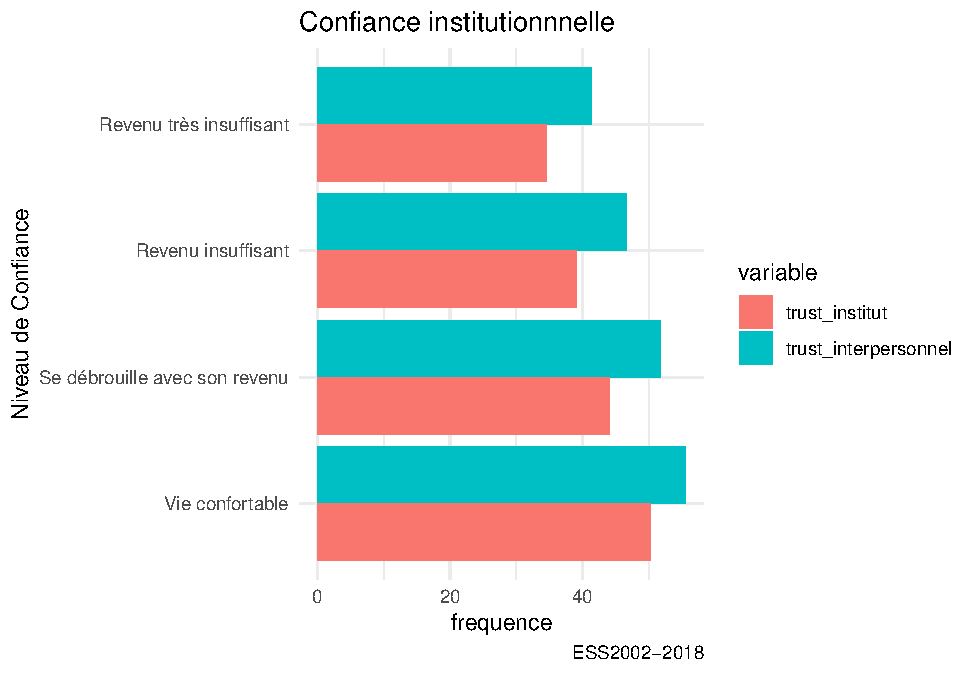
\includegraphics{bookdown-demo_files/figure-latex/0420-1.pdf}

On a une solution mais pas la meilleure, on perd l'idée de variance et ce serait bien d'ajouter des barres d'intervalle de confiances , un diagramme en lignes serait plus élégant. On en profite pour corriger l'aspect des labels peu lisibles en les inclinants, et à choisir une échelle qui omettent les valeur supérieur à 70 et inférieure à 30 pour donner une vision plus respectueuses de la totalité de l'échelle qui va de 0 à 100.

Au passage on emploie à nouveau cowplot pour combiner les graphes, et ici plus précisément partager la légende des deux graphiques.

On observera que si le niveau de confiance diminue avec le revenu, la confiance interpersonnelle est plus forte, et de manière parallèle, à la confiance institutionnelle. On remarquera enfin que c'est pour les revenu les plus faibles que l'estimation est la plus imprécise ou la variance la plus grande.

\begin{Shaded}
\begin{Highlighting}[]
\NormalTok{df\_wave2}\OtherTok{\textless{}{-}}\NormalTok{df }\SpecialCharTok{\%\textgreater{}\%} 
  \FunctionTok{filter}\NormalTok{(cntry}\SpecialCharTok{==}\StringTok{"FR"} \SpecialCharTok{\&}\NormalTok{ Year}\SpecialCharTok{==}\StringTok{"2018"}\NormalTok{)}\SpecialCharTok{\%\textgreater{}\%}
  \FunctionTok{group\_by}\NormalTok{(revenu) }\SpecialCharTok{\%\textgreater{}\%} 
  \FunctionTok{mutate}\NormalTok{(}\AttributeTok{n=}\DecValTok{1}\NormalTok{) }\SpecialCharTok{\%\textgreater{}\%}
  \FunctionTok{summarise}\NormalTok{(}\AttributeTok{trust\_interpersonnel\_se=}\FunctionTok{sd}\NormalTok{(trust\_interpersonnel, }\AttributeTok{na.rm=}\ConstantTok{TRUE}\NormalTok{), }\CommentTok{\#on calcule l\textquotesingle{}écartype des deux variables}
            \AttributeTok{trust\_institut\_se =}\FunctionTok{sd}\NormalTok{(trust\_institut, }\AttributeTok{na.rm=}\ConstantTok{TRUE}\NormalTok{),}
            \AttributeTok{n=}\FunctionTok{sum}\NormalTok{(n),}
            \AttributeTok{trust\_interpersonnel\_se=} \DecValTok{2}\SpecialCharTok{*}\NormalTok{trust\_interpersonnel\_se}\SpecialCharTok{/}\FunctionTok{sqrt}\NormalTok{(n), }\CommentTok{\# on calcule l\textquotesingle{}erreur type d\textquotesingle{}échantillonnage}
            \AttributeTok{trust\_institut\_se=}\DecValTok{2}\SpecialCharTok{*}\NormalTok{trust\_institut\_se}\SpecialCharTok{/}\FunctionTok{sqrt}\NormalTok{(n)}
\NormalTok{            ) }\SpecialCharTok{\%\textgreater{}\%}\NormalTok{ dplyr}\SpecialCharTok{::}\FunctionTok{select}\NormalTok{(}\SpecialCharTok{{-}}\NormalTok{n) }\SpecialCharTok{\%\textgreater{}\%}
  \FunctionTok{filter}\NormalTok{(}\SpecialCharTok{!}\FunctionTok{is.na}\NormalTok{(revenu)) }\SpecialCharTok{\%\textgreater{}\%} 
  \FunctionTok{gather}\NormalTok{(variable, value, }\SpecialCharTok{{-}}\NormalTok{revenu) }\SpecialCharTok{\%\textgreater{}\%} \CommentTok{\#on passe en format long}
\NormalTok{  dplyr}\SpecialCharTok{::}\FunctionTok{select}\NormalTok{(}\SpecialCharTok{{-}}\NormalTok{revenu,}\SpecialCharTok{{-}}\NormalTok{variable)}\SpecialCharTok{\%\textgreater{}\%}
  \FunctionTok{rename}\NormalTok{(}\AttributeTok{se=}\NormalTok{value)}
  
\NormalTok{df\_wave3}\OtherTok{\textless{}{-}}\FunctionTok{cbind}\NormalTok{(df\_wave,df\_wave2) }\CommentTok{\#on concatène les moyennes et les erreurs types}

\CommentTok{\#on peut enfin produire le graphique}

\NormalTok{g06a}\OtherTok{\textless{}{-}}\FunctionTok{ggplot}\NormalTok{(df\_wave3,}\FunctionTok{aes}\NormalTok{(}\AttributeTok{x=}\NormalTok{revenu,}\AttributeTok{y=}\NormalTok{value, }\AttributeTok{group=}\NormalTok{variable))}\SpecialCharTok{+}
  \FunctionTok{geom\_line}\NormalTok{(}\AttributeTok{stat=}\StringTok{"identity"}\NormalTok{,}\FunctionTok{aes}\NormalTok{(}\AttributeTok{color=}\NormalTok{variable), }\AttributeTok{size=}\FloatTok{1.5}\NormalTok{)}\SpecialCharTok{+} 
  \FunctionTok{geom\_errorbar}\NormalTok{(}\FunctionTok{aes}\NormalTok{(}\AttributeTok{ymin=}\NormalTok{value}\SpecialCharTok{{-}}\NormalTok{se, }\AttributeTok{ymax=}\NormalTok{value}\SpecialCharTok{+}\NormalTok{se, }\AttributeTok{color=}\NormalTok{variable), }\AttributeTok{width=}\NormalTok{.}\DecValTok{2}\NormalTok{,}\AttributeTok{position=}\FunctionTok{position\_dodge}\NormalTok{(}\DecValTok{0}\NormalTok{))}\SpecialCharTok{+}
  \FunctionTok{labs}\NormalTok{(}\AttributeTok{title=} \StringTok{"Confiance et revenu"}\NormalTok{,}\AttributeTok{y=} \StringTok{"Moyenne"}\NormalTok{,}\AttributeTok{x=}\ConstantTok{NULL}\NormalTok{)}\SpecialCharTok{+}
  \FunctionTok{theme}\NormalTok{(}\AttributeTok{axis.text.x =} \FunctionTok{element\_text}\NormalTok{( }\AttributeTok{angle=}\DecValTok{45}\NormalTok{, }\AttributeTok{hjust =}\DecValTok{1}\NormalTok{)) }\CommentTok{\#on controle l\textquotesingle{}angle et la position horizontale du label}

  
\NormalTok{g06b}\OtherTok{\textless{}{-}}\FunctionTok{ggplot}\NormalTok{(df\_wave3,}\FunctionTok{aes}\NormalTok{(}\AttributeTok{x=}\NormalTok{revenu,}\AttributeTok{y=}\NormalTok{value, }\AttributeTok{group=}\NormalTok{variable))}\SpecialCharTok{+}
  \FunctionTok{geom\_line}\NormalTok{(}\AttributeTok{stat=}\StringTok{"identity"}\NormalTok{,}\FunctionTok{aes}\NormalTok{(}\AttributeTok{color=}\NormalTok{variable), }\AttributeTok{size=}\FloatTok{1.5}\NormalTok{)}\SpecialCharTok{+} 
  \FunctionTok{geom\_errorbar}\NormalTok{(}\FunctionTok{aes}\NormalTok{(}\AttributeTok{ymin=}\NormalTok{value}\SpecialCharTok{{-}}\NormalTok{se, }\AttributeTok{ymax=}\NormalTok{value}\SpecialCharTok{+}\NormalTok{se, }\AttributeTok{color=}\NormalTok{variable), }\AttributeTok{width=}\NormalTok{.}\DecValTok{2}\NormalTok{,}\AttributeTok{position=}\FunctionTok{position\_dodge}\NormalTok{(}\DecValTok{0}\NormalTok{))}\SpecialCharTok{+}
  \FunctionTok{ylim}\NormalTok{(}\DecValTok{0}\NormalTok{,}\DecValTok{100}\NormalTok{)}\SpecialCharTok{+}
  \FunctionTok{labs}\NormalTok{(}\AttributeTok{title=} \StringTok{""}\NormalTok{,}\AttributeTok{y=} \StringTok{"Moyenne"}\NormalTok{,}\AttributeTok{x=}\ConstantTok{NULL}\NormalTok{)}\SpecialCharTok{+}
  \FunctionTok{theme}\NormalTok{(}\AttributeTok{axis.text.x =} \FunctionTok{element\_text}\NormalTok{( }\AttributeTok{angle=}\DecValTok{45}\NormalTok{, }\AttributeTok{hjust =}\DecValTok{1}\NormalTok{)) }\CommentTok{\#on controle l\textquotesingle{}angle et la position horizontale du label}

\NormalTok{prow }\OtherTok{\textless{}{-}} \FunctionTok{plot\_grid}\NormalTok{(}
\NormalTok{  g06a }\SpecialCharTok{+} \FunctionTok{theme}\NormalTok{(}\AttributeTok{legend.position=}\StringTok{"none"}\NormalTok{),}
\NormalTok{  g06b }\SpecialCharTok{+} \FunctionTok{theme}\NormalTok{(}\AttributeTok{legend.position=}\StringTok{"none"}\NormalTok{),}
  \AttributeTok{align =} \StringTok{\textquotesingle{}vh\textquotesingle{}}\NormalTok{,}
  \AttributeTok{labels =} \FunctionTok{c}\NormalTok{(}\StringTok{"A"}\NormalTok{, }\StringTok{"B"}\NormalTok{, }\StringTok{"C"}\NormalTok{),}
  \AttributeTok{hjust =} \SpecialCharTok{{-}}\DecValTok{1}\NormalTok{,}
  \AttributeTok{nrow =} \DecValTok{1}
\NormalTok{)}
\CommentTok{\# extract a legend that is laid out horizontally}
\NormalTok{legend\_b }\OtherTok{\textless{}{-}} \FunctionTok{get\_legend}\NormalTok{(}
\NormalTok{  g06a }\SpecialCharTok{+} 
    \FunctionTok{guides}\NormalTok{(}\AttributeTok{color =} \FunctionTok{guide\_legend}\NormalTok{(}\AttributeTok{nrow =} \DecValTok{1}\NormalTok{)) }\SpecialCharTok{+}
    \FunctionTok{theme}\NormalTok{(}\AttributeTok{legend.position =} \StringTok{"bottom"}\NormalTok{)}
\NormalTok{)}

\CommentTok{\# add the legend underneath the row we made earlier. Give it 10\%}
\CommentTok{\# of the height of one plot (via rel\_heights).}
\FunctionTok{plot\_grid}\NormalTok{(prow, legend\_b, }\AttributeTok{ncol =} \DecValTok{1}\NormalTok{, }\AttributeTok{rel\_heights =} \FunctionTok{c}\NormalTok{(}\DecValTok{1}\NormalTok{, .}\DecValTok{1}\NormalTok{))}
\end{Highlighting}
\end{Shaded}

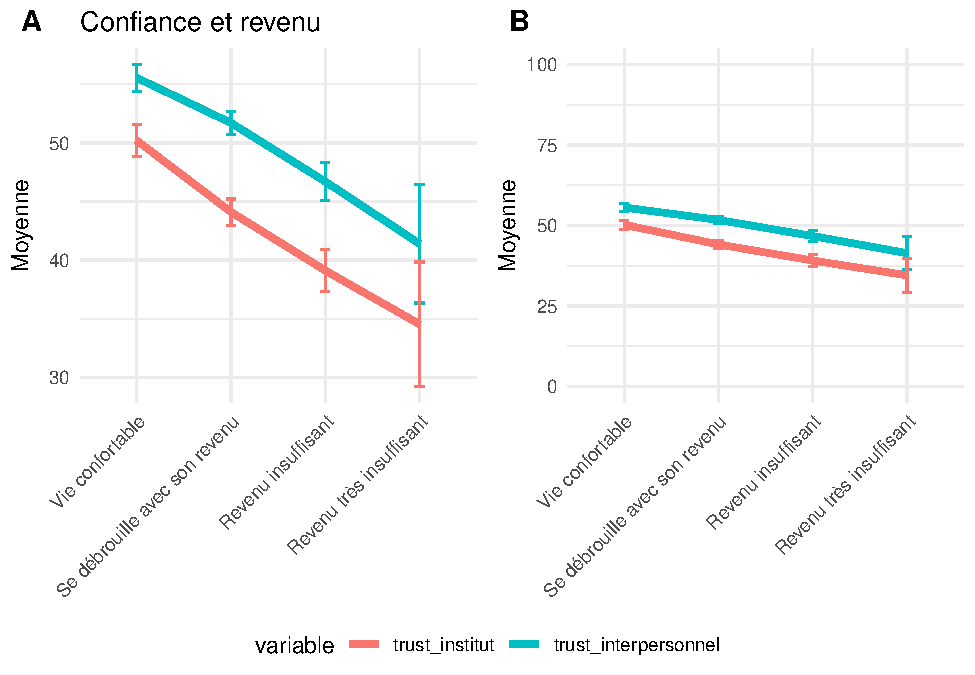
\includegraphics{bookdown-demo_files/figure-latex/0422-1.pdf}

La visualisation est utile, encore faut-il qu'on soit bien certain que les variations ne soit pas le produit du hasard, des fluctuations d'échantillonnage. Si en moyenne la perception du pouvoir d'achat est associée à des moyennes de confiance décroissantes, les différences observées sont-elle significatives? Dans les représentations précédentes c'est le choix de l'échelle qui oriente l'analyse.

On a un besoin d'un test plus objectif. Celui est le très classique test d'analyse de variance (ANOVA).

Celui-çi est le test d'analyse de variance qui consiste à comparer la variance à l'intérieur des groupes ( intra), et la variance entre les moyennes des groupes (inter ou between).

On note qu'ici on introduit la méthode flextable pour présenter des tableaux au formats scientifique. L'astuce ici est d'utiliser aussi xtable.

\begin{Shaded}
\begin{Highlighting}[]
\NormalTok{foo}\OtherTok{\textless{}{-}}\NormalTok{df }\SpecialCharTok{\%\textgreater{}\%} 
  \FunctionTok{filter}\NormalTok{(cntry}\SpecialCharTok{==}\StringTok{"FR"} \SpecialCharTok{\&}\NormalTok{ Year}\SpecialCharTok{==}\StringTok{"2018"}\NormalTok{) }\SpecialCharTok{\%\textgreater{}\%} 
  \FunctionTok{drop\_na}\NormalTok{() }\CommentTok{\#selection des données}

\NormalTok{fit}\OtherTok{\textless{}{-}}\FunctionTok{lm}\NormalTok{(trust\_institut}\SpecialCharTok{\textasciitilde{}}\NormalTok{revenu, foo) }\CommentTok{\#calcul du modèle linéaire}

\FunctionTok{anova}\NormalTok{(fit) }\CommentTok{\#test d\textquotesingle{}analyse de variance}
\end{Highlighting}
\end{Shaded}

\begin{verbatim}
## Analysis of Variance Table
## 
## Response: trust_institut
##             Df Sum Sq Mean Sq F value    Pr(>F)    
## revenu       3  27651  9217.1  32.052 < 2.2e-16 ***
## Residuals 1686 484846   287.6                      
## ---
## Signif. codes:  0 '***' 0.001 '**' 0.01 '*' 0.05 '.' 0.1 ' ' 1
\end{verbatim}

\begin{Shaded}
\begin{Highlighting}[]
\FunctionTok{library}\NormalTok{(xtable) }\CommentTok{\#xtable transforme en table certains type d\textquotesingle{}objet dont les résultats de l\textquotesingle{}anova}
\NormalTok{ft }\OtherTok{\textless{}{-}} \FunctionTok{xtable\_to\_flextable}\NormalTok{(}\FunctionTok{xtable}\NormalTok{(}\FunctionTok{anova}\NormalTok{(fit)), }\AttributeTok{hline.after =} \FunctionTok{c}\NormalTok{(}\DecValTok{0}\NormalTok{,}\DecValTok{2}\NormalTok{)) }\CommentTok{\#la fonction permet d\textquotesingle{}exploiter flextable.}
\NormalTok{ft}
\end{Highlighting}
\end{Shaded}

\providecommand{\docline}[3]{\noalign{\global\setlength{\arrayrulewidth}{#1}}\arrayrulecolor[HTML]{#2}\cline{#3}}

\setlength{\tabcolsep}{2pt}

\renewcommand*{\arraystretch}{1.5}

\begin{longtable}[c]{|p{1.01in}|p{0.67in}|p{0.96in}|p{0.91in}|p{0.81in}|p{0.73in}}



\hhline{~~~~~~}

\multicolumn{1}{!{\color[HTML]{000000}\vrule width 0pt}>{\raggedright}p{\dimexpr 1.01in+0\tabcolsep+0\arrayrulewidth}}{\fontsize{11}{11}\selectfont{\textcolor[HTML]{000000}{\global\setmainfont{Arial}{\textbf{}}}}} & \multicolumn{1}{!{\color[HTML]{000000}\vrule width 0pt}>{\raggedleft}p{\dimexpr 0.67in+0\tabcolsep+0\arrayrulewidth}}{\fontsize{11}{11}\selectfont{\textcolor[HTML]{000000}{\global\setmainfont{Arial}{\textbf{Df}}}}} & \multicolumn{1}{!{\color[HTML]{000000}\vrule width 0pt}>{\raggedleft}p{\dimexpr 0.96in+0\tabcolsep+0\arrayrulewidth}}{\fontsize{11}{11}\selectfont{\textcolor[HTML]{000000}{\global\setmainfont{Arial}{\textbf{Sum\ Sq}}}}} & \multicolumn{1}{!{\color[HTML]{000000}\vrule width 0pt}>{\raggedleft}p{\dimexpr 0.91in+0\tabcolsep+0\arrayrulewidth}}{\fontsize{11}{11}\selectfont{\textcolor[HTML]{000000}{\global\setmainfont{Arial}{\textbf{Mean\ Sq}}}}} & \multicolumn{1}{!{\color[HTML]{000000}\vrule width 0pt}>{\raggedleft}p{\dimexpr 0.81in+0\tabcolsep+0\arrayrulewidth}}{\fontsize{11}{11}\selectfont{\textcolor[HTML]{000000}{\global\setmainfont{Arial}{\textbf{F\ value}}}}} & \multicolumn{1}{!{\color[HTML]{000000}\vrule width 0pt}>{\raggedleft}p{\dimexpr 0.73in+0\tabcolsep+0\arrayrulewidth}!{\color[HTML]{000000}\vrule width 0pt}}{\fontsize{11}{11}\selectfont{\textcolor[HTML]{000000}{\global\setmainfont{Arial}{\textbf{Pr(>F)}}}}} \\

\noalign{\global\setlength{\arrayrulewidth}{1pt}}\arrayrulecolor[HTML]{000000}\cline{1-6}

\endfirsthead

\hhline{~~~~~~}

\multicolumn{1}{!{\color[HTML]{000000}\vrule width 0pt}>{\raggedright}p{\dimexpr 1.01in+0\tabcolsep+0\arrayrulewidth}}{\fontsize{11}{11}\selectfont{\textcolor[HTML]{000000}{\global\setmainfont{Arial}{\textbf{}}}}} & \multicolumn{1}{!{\color[HTML]{000000}\vrule width 0pt}>{\raggedleft}p{\dimexpr 0.67in+0\tabcolsep+0\arrayrulewidth}}{\fontsize{11}{11}\selectfont{\textcolor[HTML]{000000}{\global\setmainfont{Arial}{\textbf{Df}}}}} & \multicolumn{1}{!{\color[HTML]{000000}\vrule width 0pt}>{\raggedleft}p{\dimexpr 0.96in+0\tabcolsep+0\arrayrulewidth}}{\fontsize{11}{11}\selectfont{\textcolor[HTML]{000000}{\global\setmainfont{Arial}{\textbf{Sum\ Sq}}}}} & \multicolumn{1}{!{\color[HTML]{000000}\vrule width 0pt}>{\raggedleft}p{\dimexpr 0.91in+0\tabcolsep+0\arrayrulewidth}}{\fontsize{11}{11}\selectfont{\textcolor[HTML]{000000}{\global\setmainfont{Arial}{\textbf{Mean\ Sq}}}}} & \multicolumn{1}{!{\color[HTML]{000000}\vrule width 0pt}>{\raggedleft}p{\dimexpr 0.81in+0\tabcolsep+0\arrayrulewidth}}{\fontsize{11}{11}\selectfont{\textcolor[HTML]{000000}{\global\setmainfont{Arial}{\textbf{F\ value}}}}} & \multicolumn{1}{!{\color[HTML]{000000}\vrule width 0pt}>{\raggedleft}p{\dimexpr 0.73in+0\tabcolsep+0\arrayrulewidth}!{\color[HTML]{000000}\vrule width 0pt}}{\fontsize{11}{11}\selectfont{\textcolor[HTML]{000000}{\global\setmainfont{Arial}{\textbf{Pr(>F)}}}}} \\

\noalign{\global\setlength{\arrayrulewidth}{1pt}}\arrayrulecolor[HTML]{000000}\cline{1-6}\endhead



\multicolumn{1}{!{\color[HTML]{000000}\vrule width 0pt}>{\raggedright}p{\dimexpr 1.01in+0\tabcolsep+0\arrayrulewidth}}{\fontsize{11}{11}\selectfont{\textcolor[HTML]{000000}{\global\setmainfont{Arial}{\textbf{revenu}}}}} & \multicolumn{1}{!{\color[HTML]{000000}\vrule width 0pt}>{\raggedleft}p{\dimexpr 0.67in+0\tabcolsep+0\arrayrulewidth}}{\fontsize{11}{11}\selectfont{\textcolor[HTML]{000000}{\global\setmainfont{Arial}{3}}}} & \multicolumn{1}{!{\color[HTML]{000000}\vrule width 0pt}>{\raggedleft}p{\dimexpr 0.96in+0\tabcolsep+0\arrayrulewidth}}{\fontsize{11}{11}\selectfont{\textcolor[HTML]{000000}{\global\setmainfont{Arial}{27,651.4}}}} & \multicolumn{1}{!{\color[HTML]{000000}\vrule width 0pt}>{\raggedleft}p{\dimexpr 0.91in+0\tabcolsep+0\arrayrulewidth}}{\fontsize{11}{11}\selectfont{\textcolor[HTML]{000000}{\global\setmainfont{Arial}{9,217.1}}}} & \multicolumn{1}{!{\color[HTML]{000000}\vrule width 0pt}>{\raggedleft}p{\dimexpr 0.81in+0\tabcolsep+0\arrayrulewidth}}{\fontsize{11}{11}\selectfont{\textcolor[HTML]{000000}{\global\setmainfont{Arial}{32.1}}}} & \multicolumn{1}{!{\color[HTML]{000000}\vrule width 0pt}>{\raggedleft}p{\dimexpr 0.73in+0\tabcolsep+0\arrayrulewidth}!{\color[HTML]{000000}\vrule width 0pt}}{\fontsize{11}{11}\selectfont{\textcolor[HTML]{000000}{\global\setmainfont{Arial}{0.0}}}} \\





\multicolumn{1}{!{\color[HTML]{000000}\vrule width 0pt}>{\raggedright}p{\dimexpr 1.01in+0\tabcolsep+0\arrayrulewidth}}{\fontsize{11}{11}\selectfont{\textcolor[HTML]{000000}{\global\setmainfont{Arial}{\textbf{Residuals}}}}} & \multicolumn{1}{!{\color[HTML]{000000}\vrule width 0pt}>{\raggedleft}p{\dimexpr 0.67in+0\tabcolsep+0\arrayrulewidth}}{\fontsize{11}{11}\selectfont{\textcolor[HTML]{000000}{\global\setmainfont{Arial}{1,686}}}} & \multicolumn{1}{!{\color[HTML]{000000}\vrule width 0pt}>{\raggedleft}p{\dimexpr 0.96in+0\tabcolsep+0\arrayrulewidth}}{\fontsize{11}{11}\selectfont{\textcolor[HTML]{000000}{\global\setmainfont{Arial}{484,845.7}}}} & \multicolumn{1}{!{\color[HTML]{000000}\vrule width 0pt}>{\raggedleft}p{\dimexpr 0.91in+0\tabcolsep+0\arrayrulewidth}}{\fontsize{11}{11}\selectfont{\textcolor[HTML]{000000}{\global\setmainfont{Arial}{287.6}}}} & \multicolumn{1}{!{\color[HTML]{000000}\vrule width 0pt}>{\raggedleft}p{\dimexpr 0.81in+0\tabcolsep+0\arrayrulewidth}}{\fontsize{11}{11}\selectfont{\textcolor[HTML]{000000}{\global\setmainfont{Arial}{}}}} & \multicolumn{1}{!{\color[HTML]{000000}\vrule width 0pt}>{\raggedleft}p{\dimexpr 0.73in+0\tabcolsep+0\arrayrulewidth}!{\color[HTML]{000000}\vrule width 0pt}}{\fontsize{11}{11}\selectfont{\textcolor[HTML]{000000}{\global\setmainfont{Arial}{}}}} \\

\noalign{\global\setlength{\arrayrulewidth}{1pt}}\arrayrulecolor[HTML]{000000}\cline{1-6}



\end{longtable}

\hypertarget{deux-variables-qualitatives}{%
\subsection{Deux variables qualitatives}\label{deux-variables-qualitatives}}

L'étude de la relation éventuelle entre deux variables qualitative s'apprécie traditionnellement par une méthode de tableau croisé.

\hypertarget{tableau-croisuxe9}{%
\subsubsection{Tableau croisé}\label{tableau-croisuxe9}}

Pour calculer le tableau croisé on utilise la fonction très simple \texttt{table} et la fonction \texttt{prop.table}

\begin{Shaded}
\begin{Highlighting}[]
\NormalTok{t}\OtherTok{\textless{}{-}}\FunctionTok{table}\NormalTok{(foo}\SpecialCharTok{$}\NormalTok{revenu,foo}\SpecialCharTok{$}\NormalTok{habitat)}
\NormalTok{t}
\end{Highlighting}
\end{Shaded}

\begin{verbatim}
##                                
##                                 Big city Suburbs Town Village Countryside
##   Vie confortable                    118      82  161     142          31
##   Se débrouille avec son revenu      120     109  275     227          58
##   Revenu insuffisant                  48      38  129      88          22
##   Revenu très insuffisant              9       5   18      10           0
\end{verbatim}

\begin{Shaded}
\begin{Highlighting}[]
\FunctionTok{prop.table}\NormalTok{(t,}\DecValTok{2}\NormalTok{)}
\end{Highlighting}
\end{Shaded}

\begin{verbatim}
##                                
##                                   Big city    Suburbs       Town    Village
##   Vie confortable               0.40000000 0.35042735 0.27615780 0.30406852
##   Se débrouille avec son revenu 0.40677966 0.46581197 0.47169811 0.48608137
##   Revenu insuffisant            0.16271186 0.16239316 0.22126930 0.18843683
##   Revenu très insuffisant       0.03050847 0.02136752 0.03087479 0.02141328
##                                
##                                 Countryside
##   Vie confortable                0.27927928
##   Se débrouille avec son revenu  0.52252252
##   Revenu insuffisant             0.19819820
##   Revenu très insuffisant        0.00000000
\end{verbatim}

Mais ce n'est pas esthétique, avec la fonction \texttt{proc\_freq} de flextable on obtient une meilleure présentation. Elle nous donne en peu de mots les effectif par cellule, les pourcentages en lignes, et en colonnes.

\begin{Shaded}
\begin{Highlighting}[]
\NormalTok{ft1}\OtherTok{\textless{}{-}} \FunctionTok{proc\_freq}\NormalTok{(foo, }\StringTok{"revenu"}\NormalTok{, }\StringTok{"habitat"}\NormalTok{, }\AttributeTok{include.table\_percent =} \ConstantTok{FALSE}\NormalTok{,}
                \AttributeTok{include.row\_percent =} \ConstantTok{FALSE}\NormalTok{, }\AttributeTok{include.column\_total =} \ConstantTok{FALSE}\NormalTok{,}
  \AttributeTok{include.column\_percent =} \ConstantTok{TRUE}\NormalTok{)}
\NormalTok{ft1}
\end{Highlighting}
\end{Shaded}

\providecommand{\docline}[3]{\noalign{\global\setlength{\arrayrulewidth}{#1}}\arrayrulecolor[HTML]{#2}\cline{#3}}

\setlength{\tabcolsep}{2pt}

\renewcommand*{\arraystretch}{1.5}

\begin{longtable}[c]{|p{2.34in}|p{1.01in}|p{1.26in}|p{1.26in}|p{1.26in}|p{1.26in}|p{1.10in}|p{0.62in}}



\hhline{~~~~~~~~}

\multicolumn{2}{!{\color[HTML]{FFFFFF}\vrule width 0pt}>{\centering}p{\dimexpr 3.35in+2\tabcolsep+1\arrayrulewidth}}{\fontsize{11}{11}\selectfont{\textcolor[HTML]{000000}{\global\setmainfont{Arial}{\textbf{}}}}} & \multicolumn{6}{!{\color[HTML]{FFFFFF}\vrule width 0pt}>{\centering}p{\dimexpr 6.77in+10\tabcolsep+5\arrayrulewidth}!{\color[HTML]{FFFFFF}\vrule width 0pt}}{\fontsize{11}{11}\selectfont{\textcolor[HTML]{000000}{\global\setmainfont{Arial}{\textbf{habitat}}}}} \\

\noalign{\global\setlength{\arrayrulewidth}{1pt}}\arrayrulecolor[HTML]{000000}\cline{1-8}

\multicolumn{1}{!{\color[HTML]{000000}\vrule width 0pt}>{\centering}p{\dimexpr 2.34in+0\tabcolsep+0\arrayrulewidth}}{\fontsize{11}{11}\selectfont{\textcolor[HTML]{000000}{\global\setmainfont{Arial}{\textbf{revenu}}}}} & \multicolumn{1}{!{\color[HTML]{000000}\vrule width 0pt}>{\centering}p{\dimexpr 1.01in+0\tabcolsep+0\arrayrulewidth}}{\fontsize{11}{11}\selectfont{\textcolor[HTML]{000000}{\global\setmainfont{Arial}{\textbf{label}}}}} & \multicolumn{1}{!{\color[HTML]{000000}\vrule width 0pt}>{\centering}p{\dimexpr 1.26in+0\tabcolsep+0\arrayrulewidth}}{\fontsize{11}{11}\selectfont{\textcolor[HTML]{000000}{\global\setmainfont{Arial}{\textbf{Big\ city}}}}} & \multicolumn{1}{!{\color[HTML]{000000}\vrule width 0pt}>{\centering}p{\dimexpr 1.26in+0\tabcolsep+0\arrayrulewidth}}{\fontsize{11}{11}\selectfont{\textcolor[HTML]{000000}{\global\setmainfont{Arial}{\textbf{Suburbs}}}}} & \multicolumn{1}{!{\color[HTML]{000000}\vrule width 0pt}>{\centering}p{\dimexpr 1.26in+0\tabcolsep+0\arrayrulewidth}}{\fontsize{11}{11}\selectfont{\textcolor[HTML]{000000}{\global\setmainfont{Arial}{\textbf{Town}}}}} & \multicolumn{1}{!{\color[HTML]{000000}\vrule width 0pt}>{\centering}p{\dimexpr 1.26in+0\tabcolsep+0\arrayrulewidth}}{\fontsize{11}{11}\selectfont{\textcolor[HTML]{000000}{\global\setmainfont{Arial}{\textbf{Village}}}}} & \multicolumn{1}{!{\color[HTML]{000000}\vrule width 0pt}>{\centering}p{\dimexpr 1.1in+0\tabcolsep+0\arrayrulewidth}}{\fontsize{11}{11}\selectfont{\textcolor[HTML]{000000}{\global\setmainfont{Arial}{\textbf{Countryside}}}}} & \multicolumn{1}{!{\color[HTML]{000000}\vrule width 0pt}>{\centering}p{\dimexpr 0.62in+0\tabcolsep+0\arrayrulewidth}!{\color[HTML]{000000}\vrule width 0pt}}{\fontsize{11}{11}\selectfont{\textcolor[HTML]{000000}{\global\setmainfont{Arial}{\textbf{Total}}}}} \\

\noalign{\global\setlength{\arrayrulewidth}{2pt}}\arrayrulecolor[HTML]{000000}\cline{1-8}

\endfirsthead

\hhline{~~~~~~~~}

\multicolumn{2}{!{\color[HTML]{FFFFFF}\vrule width 0pt}>{\centering}p{\dimexpr 3.35in+2\tabcolsep+1\arrayrulewidth}}{\fontsize{11}{11}\selectfont{\textcolor[HTML]{000000}{\global\setmainfont{Arial}{\textbf{}}}}} & \multicolumn{6}{!{\color[HTML]{FFFFFF}\vrule width 0pt}>{\centering}p{\dimexpr 6.77in+10\tabcolsep+5\arrayrulewidth}!{\color[HTML]{FFFFFF}\vrule width 0pt}}{\fontsize{11}{11}\selectfont{\textcolor[HTML]{000000}{\global\setmainfont{Arial}{\textbf{habitat}}}}} \\

\noalign{\global\setlength{\arrayrulewidth}{1pt}}\arrayrulecolor[HTML]{000000}\cline{1-8}



\multicolumn{1}{!{\color[HTML]{000000}\vrule width 0pt}>{\centering}p{\dimexpr 2.34in+0\tabcolsep+0\arrayrulewidth}}{\fontsize{11}{11}\selectfont{\textcolor[HTML]{000000}{\global\setmainfont{Arial}{\textbf{revenu}}}}} & \multicolumn{1}{!{\color[HTML]{000000}\vrule width 0pt}>{\centering}p{\dimexpr 1.01in+0\tabcolsep+0\arrayrulewidth}}{\fontsize{11}{11}\selectfont{\textcolor[HTML]{000000}{\global\setmainfont{Arial}{\textbf{label}}}}} & \multicolumn{1}{!{\color[HTML]{000000}\vrule width 0pt}>{\centering}p{\dimexpr 1.26in+0\tabcolsep+0\arrayrulewidth}}{\fontsize{11}{11}\selectfont{\textcolor[HTML]{000000}{\global\setmainfont{Arial}{\textbf{Big\ city}}}}} & \multicolumn{1}{!{\color[HTML]{000000}\vrule width 0pt}>{\centering}p{\dimexpr 1.26in+0\tabcolsep+0\arrayrulewidth}}{\fontsize{11}{11}\selectfont{\textcolor[HTML]{000000}{\global\setmainfont{Arial}{\textbf{Suburbs}}}}} & \multicolumn{1}{!{\color[HTML]{000000}\vrule width 0pt}>{\centering}p{\dimexpr 1.26in+0\tabcolsep+0\arrayrulewidth}}{\fontsize{11}{11}\selectfont{\textcolor[HTML]{000000}{\global\setmainfont{Arial}{\textbf{Town}}}}} & \multicolumn{1}{!{\color[HTML]{000000}\vrule width 0pt}>{\centering}p{\dimexpr 1.26in+0\tabcolsep+0\arrayrulewidth}}{\fontsize{11}{11}\selectfont{\textcolor[HTML]{000000}{\global\setmainfont{Arial}{\textbf{Village}}}}} & \multicolumn{1}{!{\color[HTML]{000000}\vrule width 0pt}>{\centering}p{\dimexpr 1.1in+0\tabcolsep+0\arrayrulewidth}}{\fontsize{11}{11}\selectfont{\textcolor[HTML]{000000}{\global\setmainfont{Arial}{\textbf{Countryside}}}}} & \multicolumn{1}{!{\color[HTML]{000000}\vrule width 0pt}>{\centering}p{\dimexpr 0.62in+0\tabcolsep+0\arrayrulewidth}!{\color[HTML]{000000}\vrule width 0pt}}{\fontsize{11}{11}\selectfont{\textcolor[HTML]{000000}{\global\setmainfont{Arial}{\textbf{Total}}}}} \\

\noalign{\global\setlength{\arrayrulewidth}{2pt}}\arrayrulecolor[HTML]{000000}\cline{1-8}\endhead



\multicolumn{1}{!{\color[HTML]{000000}\vrule width 0pt}>{\centering}p{\dimexpr 2.34in+0\tabcolsep+0\arrayrulewidth}}{} & \multicolumn{1}{!{\color[HTML]{000000}\vrule width 0pt}>{\centering}p{\dimexpr 1.01in+0\tabcolsep+0\arrayrulewidth}}{\fontsize{11}{11}\selectfont{\textcolor[HTML]{000000}{\global\setmainfont{Arial}{Frequency}}}} & \multicolumn{1}{!{\color[HTML]{000000}\vrule width 0pt}>{\centering}p{\dimexpr 1.26in+0\tabcolsep+0\arrayrulewidth}}{\fontsize{11}{11}\selectfont{\textcolor[HTML]{000000}{\global\setmainfont{Arial}{118}}}} & \multicolumn{1}{!{\color[HTML]{000000}\vrule width 0pt}>{\centering}p{\dimexpr 1.26in+0\tabcolsep+0\arrayrulewidth}}{\fontsize{11}{11}\selectfont{\textcolor[HTML]{000000}{\global\setmainfont{Arial}{82}}}} & \multicolumn{1}{!{\color[HTML]{000000}\vrule width 0pt}>{\centering}p{\dimexpr 1.26in+0\tabcolsep+0\arrayrulewidth}}{\fontsize{11}{11}\selectfont{\textcolor[HTML]{000000}{\global\setmainfont{Arial}{161}}}} & \multicolumn{1}{!{\color[HTML]{000000}\vrule width 0pt}>{\centering}p{\dimexpr 1.26in+0\tabcolsep+0\arrayrulewidth}}{\fontsize{11}{11}\selectfont{\textcolor[HTML]{000000}{\global\setmainfont{Arial}{142}}}} & \multicolumn{1}{!{\color[HTML]{000000}\vrule width 0pt}>{\centering}p{\dimexpr 1.1in+0\tabcolsep+0\arrayrulewidth}}{\fontsize{11}{11}\selectfont{\textcolor[HTML]{000000}{\global\setmainfont{Arial}{31}}}} & \multicolumn{1}{!{\color[HTML]{000000}\vrule width 0pt}>{\centering}p{\dimexpr 0.62in+0\tabcolsep+0\arrayrulewidth}!{\color[HTML]{000000}\vrule width 0pt}}{\fontsize{11}{11}\selectfont{\textcolor[HTML]{000000}{\global\setmainfont{Arial}{534}}}} \\





\multicolumn{1}{!{\color[HTML]{000000}\vrule width 0pt}>{\centering}p{\dimexpr 2.34in+0\tabcolsep+0\arrayrulewidth}}{\multirow[t]{-2}{*}{\fontsize{11}{11}\selectfont{\textcolor[HTML]{000000}{\global\setmainfont{Arial}{\textbf{Vie\ confortable}}}}}} & \multicolumn{1}{!{\color[HTML]{000000}\vrule width 0pt}>{\centering}p{\dimexpr 1.01in+0\tabcolsep+0\arrayrulewidth}}{\fontsize{11}{11}\selectfont{\textcolor[HTML]{000000}{\global\setmainfont{Arial}{Col\ Pct}}}} & \multicolumn{1}{!{\color[HTML]{000000}\vrule width 0pt}>{\centering}p{\dimexpr 1.26in+0\tabcolsep+0\arrayrulewidth}}{\fontsize{11}{11}\selectfont{\textcolor[HTML]{000000}{\global\setmainfont{Arial}{40\%}}}} & \multicolumn{1}{!{\color[HTML]{000000}\vrule width 0pt}>{\centering}p{\dimexpr 1.26in+0\tabcolsep+0\arrayrulewidth}}{\fontsize{11}{11}\selectfont{\textcolor[HTML]{000000}{\global\setmainfont{Arial}{35.04\%}}}} & \multicolumn{1}{!{\color[HTML]{000000}\vrule width 0pt}>{\centering}p{\dimexpr 1.26in+0\tabcolsep+0\arrayrulewidth}}{\fontsize{11}{11}\selectfont{\textcolor[HTML]{000000}{\global\setmainfont{Arial}{27.62\%}}}} & \multicolumn{1}{!{\color[HTML]{000000}\vrule width 0pt}>{\centering}p{\dimexpr 1.26in+0\tabcolsep+0\arrayrulewidth}}{\fontsize{11}{11}\selectfont{\textcolor[HTML]{000000}{\global\setmainfont{Arial}{30.41\%}}}} & \multicolumn{1}{!{\color[HTML]{000000}\vrule width 0pt}>{\centering}p{\dimexpr 1.1in+0\tabcolsep+0\arrayrulewidth}}{\fontsize{11}{11}\selectfont{\textcolor[HTML]{000000}{\global\setmainfont{Arial}{27.93\%}}}} & \multicolumn{1}{!{\color[HTML]{000000}\vrule width 0pt}>{\centering}p{\dimexpr 0.62in+0\tabcolsep+0\arrayrulewidth}!{\color[HTML]{000000}\vrule width 0pt}}{\fontsize{11}{11}\selectfont{\textcolor[HTML]{000000}{\global\setmainfont{Arial}{}}}} \\





\multicolumn{1}{!{\color[HTML]{000000}\vrule width 0pt}>{\centering}p{\dimexpr 2.34in+0\tabcolsep+0\arrayrulewidth}}{} & \multicolumn{1}{!{\color[HTML]{000000}\vrule width 0pt}>{\centering}p{\dimexpr 1.01in+0\tabcolsep+0\arrayrulewidth}}{\fontsize{11}{11}\selectfont{\textcolor[HTML]{000000}{\global\setmainfont{Arial}{Frequency}}}} & \multicolumn{1}{!{\color[HTML]{000000}\vrule width 0pt}>{\centering}p{\dimexpr 1.26in+0\tabcolsep+0\arrayrulewidth}}{\fontsize{11}{11}\selectfont{\textcolor[HTML]{000000}{\global\setmainfont{Arial}{120}}}} & \multicolumn{1}{!{\color[HTML]{000000}\vrule width 0pt}>{\centering}p{\dimexpr 1.26in+0\tabcolsep+0\arrayrulewidth}}{\fontsize{11}{11}\selectfont{\textcolor[HTML]{000000}{\global\setmainfont{Arial}{109}}}} & \multicolumn{1}{!{\color[HTML]{000000}\vrule width 0pt}>{\centering}p{\dimexpr 1.26in+0\tabcolsep+0\arrayrulewidth}}{\fontsize{11}{11}\selectfont{\textcolor[HTML]{000000}{\global\setmainfont{Arial}{275}}}} & \multicolumn{1}{!{\color[HTML]{000000}\vrule width 0pt}>{\centering}p{\dimexpr 1.26in+0\tabcolsep+0\arrayrulewidth}}{\fontsize{11}{11}\selectfont{\textcolor[HTML]{000000}{\global\setmainfont{Arial}{227}}}} & \multicolumn{1}{!{\color[HTML]{000000}\vrule width 0pt}>{\centering}p{\dimexpr 1.1in+0\tabcolsep+0\arrayrulewidth}}{\fontsize{11}{11}\selectfont{\textcolor[HTML]{000000}{\global\setmainfont{Arial}{58}}}} & \multicolumn{1}{!{\color[HTML]{000000}\vrule width 0pt}>{\centering}p{\dimexpr 0.62in+0\tabcolsep+0\arrayrulewidth}!{\color[HTML]{000000}\vrule width 0pt}}{\fontsize{11}{11}\selectfont{\textcolor[HTML]{000000}{\global\setmainfont{Arial}{789}}}} \\





\multicolumn{1}{!{\color[HTML]{000000}\vrule width 0pt}>{\centering}p{\dimexpr 2.34in+0\tabcolsep+0\arrayrulewidth}}{\multirow[t]{-2}{*}{\fontsize{11}{11}\selectfont{\textcolor[HTML]{000000}{\global\setmainfont{Arial}{\textbf{Se\ débrouille\ avec\ son\ revenu}}}}}} & \multicolumn{1}{!{\color[HTML]{000000}\vrule width 0pt}>{\centering}p{\dimexpr 1.01in+0\tabcolsep+0\arrayrulewidth}}{\fontsize{11}{11}\selectfont{\textcolor[HTML]{000000}{\global\setmainfont{Arial}{Col\ Pct}}}} & \multicolumn{1}{!{\color[HTML]{000000}\vrule width 0pt}>{\centering}p{\dimexpr 1.26in+0\tabcolsep+0\arrayrulewidth}}{\fontsize{11}{11}\selectfont{\textcolor[HTML]{000000}{\global\setmainfont{Arial}{40.68\%}}}} & \multicolumn{1}{!{\color[HTML]{000000}\vrule width 0pt}>{\centering}p{\dimexpr 1.26in+0\tabcolsep+0\arrayrulewidth}}{\fontsize{11}{11}\selectfont{\textcolor[HTML]{000000}{\global\setmainfont{Arial}{46.58\%}}}} & \multicolumn{1}{!{\color[HTML]{000000}\vrule width 0pt}>{\centering}p{\dimexpr 1.26in+0\tabcolsep+0\arrayrulewidth}}{\fontsize{11}{11}\selectfont{\textcolor[HTML]{000000}{\global\setmainfont{Arial}{47.17\%}}}} & \multicolumn{1}{!{\color[HTML]{000000}\vrule width 0pt}>{\centering}p{\dimexpr 1.26in+0\tabcolsep+0\arrayrulewidth}}{\fontsize{11}{11}\selectfont{\textcolor[HTML]{000000}{\global\setmainfont{Arial}{48.61\%}}}} & \multicolumn{1}{!{\color[HTML]{000000}\vrule width 0pt}>{\centering}p{\dimexpr 1.1in+0\tabcolsep+0\arrayrulewidth}}{\fontsize{11}{11}\selectfont{\textcolor[HTML]{000000}{\global\setmainfont{Arial}{52.25\%}}}} & \multicolumn{1}{!{\color[HTML]{000000}\vrule width 0pt}>{\centering}p{\dimexpr 0.62in+0\tabcolsep+0\arrayrulewidth}!{\color[HTML]{000000}\vrule width 0pt}}{\fontsize{11}{11}\selectfont{\textcolor[HTML]{000000}{\global\setmainfont{Arial}{}}}} \\





\multicolumn{1}{!{\color[HTML]{000000}\vrule width 0pt}>{\centering}p{\dimexpr 2.34in+0\tabcolsep+0\arrayrulewidth}}{} & \multicolumn{1}{!{\color[HTML]{000000}\vrule width 0pt}>{\centering}p{\dimexpr 1.01in+0\tabcolsep+0\arrayrulewidth}}{\fontsize{11}{11}\selectfont{\textcolor[HTML]{000000}{\global\setmainfont{Arial}{Frequency}}}} & \multicolumn{1}{!{\color[HTML]{000000}\vrule width 0pt}>{\centering}p{\dimexpr 1.26in+0\tabcolsep+0\arrayrulewidth}}{\fontsize{11}{11}\selectfont{\textcolor[HTML]{000000}{\global\setmainfont{Arial}{48}}}} & \multicolumn{1}{!{\color[HTML]{000000}\vrule width 0pt}>{\centering}p{\dimexpr 1.26in+0\tabcolsep+0\arrayrulewidth}}{\fontsize{11}{11}\selectfont{\textcolor[HTML]{000000}{\global\setmainfont{Arial}{38}}}} & \multicolumn{1}{!{\color[HTML]{000000}\vrule width 0pt}>{\centering}p{\dimexpr 1.26in+0\tabcolsep+0\arrayrulewidth}}{\fontsize{11}{11}\selectfont{\textcolor[HTML]{000000}{\global\setmainfont{Arial}{129}}}} & \multicolumn{1}{!{\color[HTML]{000000}\vrule width 0pt}>{\centering}p{\dimexpr 1.26in+0\tabcolsep+0\arrayrulewidth}}{\fontsize{11}{11}\selectfont{\textcolor[HTML]{000000}{\global\setmainfont{Arial}{88}}}} & \multicolumn{1}{!{\color[HTML]{000000}\vrule width 0pt}>{\centering}p{\dimexpr 1.1in+0\tabcolsep+0\arrayrulewidth}}{\fontsize{11}{11}\selectfont{\textcolor[HTML]{000000}{\global\setmainfont{Arial}{22}}}} & \multicolumn{1}{!{\color[HTML]{000000}\vrule width 0pt}>{\centering}p{\dimexpr 0.62in+0\tabcolsep+0\arrayrulewidth}!{\color[HTML]{000000}\vrule width 0pt}}{\fontsize{11}{11}\selectfont{\textcolor[HTML]{000000}{\global\setmainfont{Arial}{325}}}} \\





\multicolumn{1}{!{\color[HTML]{000000}\vrule width 0pt}>{\centering}p{\dimexpr 2.34in+0\tabcolsep+0\arrayrulewidth}}{\multirow[t]{-2}{*}{\fontsize{11}{11}\selectfont{\textcolor[HTML]{000000}{\global\setmainfont{Arial}{\textbf{Revenu\ insuffisant}}}}}} & \multicolumn{1}{!{\color[HTML]{000000}\vrule width 0pt}>{\centering}p{\dimexpr 1.01in+0\tabcolsep+0\arrayrulewidth}}{\fontsize{11}{11}\selectfont{\textcolor[HTML]{000000}{\global\setmainfont{Arial}{Col\ Pct}}}} & \multicolumn{1}{!{\color[HTML]{000000}\vrule width 0pt}>{\centering}p{\dimexpr 1.26in+0\tabcolsep+0\arrayrulewidth}}{\fontsize{11}{11}\selectfont{\textcolor[HTML]{000000}{\global\setmainfont{Arial}{16.27\%}}}} & \multicolumn{1}{!{\color[HTML]{000000}\vrule width 0pt}>{\centering}p{\dimexpr 1.26in+0\tabcolsep+0\arrayrulewidth}}{\fontsize{11}{11}\selectfont{\textcolor[HTML]{000000}{\global\setmainfont{Arial}{16.24\%}}}} & \multicolumn{1}{!{\color[HTML]{000000}\vrule width 0pt}>{\centering}p{\dimexpr 1.26in+0\tabcolsep+0\arrayrulewidth}}{\fontsize{11}{11}\selectfont{\textcolor[HTML]{000000}{\global\setmainfont{Arial}{22.13\%}}}} & \multicolumn{1}{!{\color[HTML]{000000}\vrule width 0pt}>{\centering}p{\dimexpr 1.26in+0\tabcolsep+0\arrayrulewidth}}{\fontsize{11}{11}\selectfont{\textcolor[HTML]{000000}{\global\setmainfont{Arial}{18.84\%}}}} & \multicolumn{1}{!{\color[HTML]{000000}\vrule width 0pt}>{\centering}p{\dimexpr 1.1in+0\tabcolsep+0\arrayrulewidth}}{\fontsize{11}{11}\selectfont{\textcolor[HTML]{000000}{\global\setmainfont{Arial}{19.82\%}}}} & \multicolumn{1}{!{\color[HTML]{000000}\vrule width 0pt}>{\centering}p{\dimexpr 0.62in+0\tabcolsep+0\arrayrulewidth}!{\color[HTML]{000000}\vrule width 0pt}}{\fontsize{11}{11}\selectfont{\textcolor[HTML]{000000}{\global\setmainfont{Arial}{}}}} \\





\multicolumn{1}{!{\color[HTML]{000000}\vrule width 0pt}>{\centering}p{\dimexpr 2.34in+0\tabcolsep+0\arrayrulewidth}}{} & \multicolumn{1}{!{\color[HTML]{000000}\vrule width 0pt}>{\centering}p{\dimexpr 1.01in+0\tabcolsep+0\arrayrulewidth}}{\fontsize{11}{11}\selectfont{\textcolor[HTML]{000000}{\global\setmainfont{Arial}{Frequency}}}} & \multicolumn{1}{!{\color[HTML]{000000}\vrule width 0pt}>{\centering}p{\dimexpr 1.26in+0\tabcolsep+0\arrayrulewidth}}{\fontsize{11}{11}\selectfont{\textcolor[HTML]{000000}{\global\setmainfont{Arial}{9}}}} & \multicolumn{1}{!{\color[HTML]{000000}\vrule width 0pt}>{\centering}p{\dimexpr 1.26in+0\tabcolsep+0\arrayrulewidth}}{\fontsize{11}{11}\selectfont{\textcolor[HTML]{000000}{\global\setmainfont{Arial}{5}}}} & \multicolumn{1}{!{\color[HTML]{000000}\vrule width 0pt}>{\centering}p{\dimexpr 1.26in+0\tabcolsep+0\arrayrulewidth}}{\fontsize{11}{11}\selectfont{\textcolor[HTML]{000000}{\global\setmainfont{Arial}{18}}}} & \multicolumn{1}{!{\color[HTML]{000000}\vrule width 0pt}>{\centering}p{\dimexpr 1.26in+0\tabcolsep+0\arrayrulewidth}}{\fontsize{11}{11}\selectfont{\textcolor[HTML]{000000}{\global\setmainfont{Arial}{10}}}} & \multicolumn{1}{!{\color[HTML]{000000}\vrule width 0pt}>{\centering}p{\dimexpr 1.1in+0\tabcolsep+0\arrayrulewidth}}{\fontsize{11}{11}\selectfont{\textcolor[HTML]{000000}{\global\setmainfont{Arial}{0}}}} & \multicolumn{1}{!{\color[HTML]{000000}\vrule width 0pt}>{\centering}p{\dimexpr 0.62in+0\tabcolsep+0\arrayrulewidth}!{\color[HTML]{000000}\vrule width 0pt}}{\fontsize{11}{11}\selectfont{\textcolor[HTML]{000000}{\global\setmainfont{Arial}{42}}}} \\





\multicolumn{1}{!{\color[HTML]{000000}\vrule width 0pt}>{\centering}p{\dimexpr 2.34in+0\tabcolsep+0\arrayrulewidth}}{\multirow[t]{-2}{*}{\fontsize{11}{11}\selectfont{\textcolor[HTML]{000000}{\global\setmainfont{Arial}{\textbf{Revenu\ très\ insuffisant}}}}}} & \multicolumn{1}{!{\color[HTML]{000000}\vrule width 0pt}>{\centering}p{\dimexpr 1.01in+0\tabcolsep+0\arrayrulewidth}}{\fontsize{11}{11}\selectfont{\textcolor[HTML]{000000}{\global\setmainfont{Arial}{Col\ Pct}}}} & \multicolumn{1}{!{\color[HTML]{000000}\vrule width 0pt}>{\centering}p{\dimexpr 1.26in+0\tabcolsep+0\arrayrulewidth}}{\fontsize{11}{11}\selectfont{\textcolor[HTML]{000000}{\global\setmainfont{Arial}{3.05\%}}}} & \multicolumn{1}{!{\color[HTML]{000000}\vrule width 0pt}>{\centering}p{\dimexpr 1.26in+0\tabcolsep+0\arrayrulewidth}}{\fontsize{11}{11}\selectfont{\textcolor[HTML]{000000}{\global\setmainfont{Arial}{2.14\%}}}} & \multicolumn{1}{!{\color[HTML]{000000}\vrule width 0pt}>{\centering}p{\dimexpr 1.26in+0\tabcolsep+0\arrayrulewidth}}{\fontsize{11}{11}\selectfont{\textcolor[HTML]{000000}{\global\setmainfont{Arial}{3.09\%}}}} & \multicolumn{1}{!{\color[HTML]{000000}\vrule width 0pt}>{\centering}p{\dimexpr 1.26in+0\tabcolsep+0\arrayrulewidth}}{\fontsize{11}{11}\selectfont{\textcolor[HTML]{000000}{\global\setmainfont{Arial}{2.14\%}}}} & \multicolumn{1}{!{\color[HTML]{000000}\vrule width 0pt}>{\centering}p{\dimexpr 1.1in+0\tabcolsep+0\arrayrulewidth}}{\fontsize{11}{11}\selectfont{\textcolor[HTML]{000000}{\global\setmainfont{Arial}{0\%}}}} & \multicolumn{1}{!{\color[HTML]{000000}\vrule width 0pt}>{\centering}p{\dimexpr 0.62in+0\tabcolsep+0\arrayrulewidth}!{\color[HTML]{000000}\vrule width 0pt}}{\fontsize{11}{11}\selectfont{\textcolor[HTML]{000000}{\global\setmainfont{Arial}{}}}} \\

\noalign{\global\setlength{\arrayrulewidth}{2pt}}\arrayrulecolor[HTML]{666666}\cline{1-8}



\end{longtable}

\begin{Shaded}
\begin{Highlighting}[]
\NormalTok{ft2}\OtherTok{\textless{}{-}} \FunctionTok{proc\_freq}\NormalTok{(foo, }\StringTok{"revenu"}\NormalTok{, }\StringTok{"habitat"}\NormalTok{, }\AttributeTok{include.table\_percent =} \ConstantTok{FALSE}\NormalTok{,}
                \AttributeTok{include.row\_percent =} \ConstantTok{TRUE}\NormalTok{,}
  \AttributeTok{include.column\_percent =} \ConstantTok{FALSE}\NormalTok{)}
\NormalTok{ft2}
\end{Highlighting}
\end{Shaded}

\providecommand{\docline}[3]{\noalign{\global\setlength{\arrayrulewidth}{#1}}\arrayrulecolor[HTML]{#2}\cline{#3}}

\setlength{\tabcolsep}{2pt}

\renewcommand*{\arraystretch}{1.5}

\begin{longtable}[c]{|p{2.34in}|p{1.01in}|p{1.18in}|p{1.18in}|p{1.18in}|p{1.18in}|p{1.26in}|p{0.67in}}



\hhline{~~~~~~~~}

\multicolumn{2}{!{\color[HTML]{FFFFFF}\vrule width 0pt}>{\centering}p{\dimexpr 3.35in+2\tabcolsep+1\arrayrulewidth}}{\fontsize{11}{11}\selectfont{\textcolor[HTML]{000000}{\global\setmainfont{Arial}{\textbf{}}}}} & \multicolumn{6}{!{\color[HTML]{FFFFFF}\vrule width 0pt}>{\centering}p{\dimexpr 6.64in+10\tabcolsep+5\arrayrulewidth}!{\color[HTML]{FFFFFF}\vrule width 0pt}}{\fontsize{11}{11}\selectfont{\textcolor[HTML]{000000}{\global\setmainfont{Arial}{\textbf{habitat}}}}} \\

\noalign{\global\setlength{\arrayrulewidth}{1pt}}\arrayrulecolor[HTML]{000000}\cline{1-8}

\multicolumn{1}{!{\color[HTML]{000000}\vrule width 0pt}>{\centering}p{\dimexpr 2.34in+0\tabcolsep+0\arrayrulewidth}}{\fontsize{11}{11}\selectfont{\textcolor[HTML]{000000}{\global\setmainfont{Arial}{\textbf{revenu}}}}} & \multicolumn{1}{!{\color[HTML]{000000}\vrule width 0pt}>{\centering}p{\dimexpr 1.01in+0\tabcolsep+0\arrayrulewidth}}{\fontsize{11}{11}\selectfont{\textcolor[HTML]{000000}{\global\setmainfont{Arial}{\textbf{label}}}}} & \multicolumn{1}{!{\color[HTML]{000000}\vrule width 0pt}>{\centering}p{\dimexpr 1.18in+0\tabcolsep+0\arrayrulewidth}}{\fontsize{11}{11}\selectfont{\textcolor[HTML]{000000}{\global\setmainfont{Arial}{\textbf{Big\ city}}}}} & \multicolumn{1}{!{\color[HTML]{000000}\vrule width 0pt}>{\centering}p{\dimexpr 1.18in+0\tabcolsep+0\arrayrulewidth}}{\fontsize{11}{11}\selectfont{\textcolor[HTML]{000000}{\global\setmainfont{Arial}{\textbf{Suburbs}}}}} & \multicolumn{1}{!{\color[HTML]{000000}\vrule width 0pt}>{\centering}p{\dimexpr 1.18in+0\tabcolsep+0\arrayrulewidth}}{\fontsize{11}{11}\selectfont{\textcolor[HTML]{000000}{\global\setmainfont{Arial}{\textbf{Town}}}}} & \multicolumn{1}{!{\color[HTML]{000000}\vrule width 0pt}>{\centering}p{\dimexpr 1.18in+0\tabcolsep+0\arrayrulewidth}}{\fontsize{11}{11}\selectfont{\textcolor[HTML]{000000}{\global\setmainfont{Arial}{\textbf{Village}}}}} & \multicolumn{1}{!{\color[HTML]{000000}\vrule width 0pt}>{\centering}p{\dimexpr 1.26in+0\tabcolsep+0\arrayrulewidth}}{\fontsize{11}{11}\selectfont{\textcolor[HTML]{000000}{\global\setmainfont{Arial}{\textbf{Countryside}}}}} & \multicolumn{1}{!{\color[HTML]{000000}\vrule width 0pt}>{\centering}p{\dimexpr 0.67in+0\tabcolsep+0\arrayrulewidth}!{\color[HTML]{000000}\vrule width 0pt}}{\fontsize{11}{11}\selectfont{\textcolor[HTML]{000000}{\global\setmainfont{Arial}{\textbf{Total}}}}} \\

\noalign{\global\setlength{\arrayrulewidth}{2pt}}\arrayrulecolor[HTML]{000000}\cline{1-8}

\endfirsthead

\hhline{~~~~~~~~}

\multicolumn{2}{!{\color[HTML]{FFFFFF}\vrule width 0pt}>{\centering}p{\dimexpr 3.35in+2\tabcolsep+1\arrayrulewidth}}{\fontsize{11}{11}\selectfont{\textcolor[HTML]{000000}{\global\setmainfont{Arial}{\textbf{}}}}} & \multicolumn{6}{!{\color[HTML]{FFFFFF}\vrule width 0pt}>{\centering}p{\dimexpr 6.64in+10\tabcolsep+5\arrayrulewidth}!{\color[HTML]{FFFFFF}\vrule width 0pt}}{\fontsize{11}{11}\selectfont{\textcolor[HTML]{000000}{\global\setmainfont{Arial}{\textbf{habitat}}}}} \\

\noalign{\global\setlength{\arrayrulewidth}{1pt}}\arrayrulecolor[HTML]{000000}\cline{1-8}



\multicolumn{1}{!{\color[HTML]{000000}\vrule width 0pt}>{\centering}p{\dimexpr 2.34in+0\tabcolsep+0\arrayrulewidth}}{\fontsize{11}{11}\selectfont{\textcolor[HTML]{000000}{\global\setmainfont{Arial}{\textbf{revenu}}}}} & \multicolumn{1}{!{\color[HTML]{000000}\vrule width 0pt}>{\centering}p{\dimexpr 1.01in+0\tabcolsep+0\arrayrulewidth}}{\fontsize{11}{11}\selectfont{\textcolor[HTML]{000000}{\global\setmainfont{Arial}{\textbf{label}}}}} & \multicolumn{1}{!{\color[HTML]{000000}\vrule width 0pt}>{\centering}p{\dimexpr 1.18in+0\tabcolsep+0\arrayrulewidth}}{\fontsize{11}{11}\selectfont{\textcolor[HTML]{000000}{\global\setmainfont{Arial}{\textbf{Big\ city}}}}} & \multicolumn{1}{!{\color[HTML]{000000}\vrule width 0pt}>{\centering}p{\dimexpr 1.18in+0\tabcolsep+0\arrayrulewidth}}{\fontsize{11}{11}\selectfont{\textcolor[HTML]{000000}{\global\setmainfont{Arial}{\textbf{Suburbs}}}}} & \multicolumn{1}{!{\color[HTML]{000000}\vrule width 0pt}>{\centering}p{\dimexpr 1.18in+0\tabcolsep+0\arrayrulewidth}}{\fontsize{11}{11}\selectfont{\textcolor[HTML]{000000}{\global\setmainfont{Arial}{\textbf{Town}}}}} & \multicolumn{1}{!{\color[HTML]{000000}\vrule width 0pt}>{\centering}p{\dimexpr 1.18in+0\tabcolsep+0\arrayrulewidth}}{\fontsize{11}{11}\selectfont{\textcolor[HTML]{000000}{\global\setmainfont{Arial}{\textbf{Village}}}}} & \multicolumn{1}{!{\color[HTML]{000000}\vrule width 0pt}>{\centering}p{\dimexpr 1.26in+0\tabcolsep+0\arrayrulewidth}}{\fontsize{11}{11}\selectfont{\textcolor[HTML]{000000}{\global\setmainfont{Arial}{\textbf{Countryside}}}}} & \multicolumn{1}{!{\color[HTML]{000000}\vrule width 0pt}>{\centering}p{\dimexpr 0.67in+0\tabcolsep+0\arrayrulewidth}!{\color[HTML]{000000}\vrule width 0pt}}{\fontsize{11}{11}\selectfont{\textcolor[HTML]{000000}{\global\setmainfont{Arial}{\textbf{Total}}}}} \\

\noalign{\global\setlength{\arrayrulewidth}{2pt}}\arrayrulecolor[HTML]{000000}\cline{1-8}\endhead



\multicolumn{1}{!{\color[HTML]{000000}\vrule width 0pt}>{\centering}p{\dimexpr 2.34in+0\tabcolsep+0\arrayrulewidth}}{} & \multicolumn{1}{!{\color[HTML]{000000}\vrule width 0pt}>{\centering}p{\dimexpr 1.01in+0\tabcolsep+0\arrayrulewidth}}{\fontsize{11}{11}\selectfont{\textcolor[HTML]{000000}{\global\setmainfont{Arial}{Frequency}}}} & \multicolumn{1}{!{\color[HTML]{000000}\vrule width 0pt}>{\centering}p{\dimexpr 1.18in+0\tabcolsep+0\arrayrulewidth}}{\fontsize{11}{11}\selectfont{\textcolor[HTML]{000000}{\global\setmainfont{Arial}{118}}}} & \multicolumn{1}{!{\color[HTML]{000000}\vrule width 0pt}>{\centering}p{\dimexpr 1.18in+0\tabcolsep+0\arrayrulewidth}}{\fontsize{11}{11}\selectfont{\textcolor[HTML]{000000}{\global\setmainfont{Arial}{82}}}} & \multicolumn{1}{!{\color[HTML]{000000}\vrule width 0pt}>{\centering}p{\dimexpr 1.18in+0\tabcolsep+0\arrayrulewidth}}{\fontsize{11}{11}\selectfont{\textcolor[HTML]{000000}{\global\setmainfont{Arial}{161}}}} & \multicolumn{1}{!{\color[HTML]{000000}\vrule width 0pt}>{\centering}p{\dimexpr 1.18in+0\tabcolsep+0\arrayrulewidth}}{\fontsize{11}{11}\selectfont{\textcolor[HTML]{000000}{\global\setmainfont{Arial}{142}}}} & \multicolumn{1}{!{\color[HTML]{000000}\vrule width 0pt}>{\centering}p{\dimexpr 1.26in+0\tabcolsep+0\arrayrulewidth}}{\fontsize{11}{11}\selectfont{\textcolor[HTML]{000000}{\global\setmainfont{Arial}{31}}}} & \multicolumn{1}{!{\color[HTML]{000000}\vrule width 0pt}>{\centering}p{\dimexpr 0.67in+0\tabcolsep+0\arrayrulewidth}!{\color[HTML]{000000}\vrule width 0pt}}{\fontsize{11}{11}\selectfont{\textcolor[HTML]{000000}{\global\setmainfont{Arial}{534}}}} \\





\multicolumn{1}{!{\color[HTML]{000000}\vrule width 0pt}>{\centering}p{\dimexpr 2.34in+0\tabcolsep+0\arrayrulewidth}}{\multirow[t]{-2}{*}{\fontsize{11}{11}\selectfont{\textcolor[HTML]{000000}{\global\setmainfont{Arial}{\textbf{Vie\ confortable}}}}}} & \multicolumn{1}{!{\color[HTML]{000000}\vrule width 0pt}>{\centering}p{\dimexpr 1.01in+0\tabcolsep+0\arrayrulewidth}}{\fontsize{11}{11}\selectfont{\textcolor[HTML]{000000}{\global\setmainfont{Arial}{Row\ Pct}}}} & \multicolumn{1}{!{\color[HTML]{000000}\vrule width 0pt}>{\centering}p{\dimexpr 1.18in+0\tabcolsep+0\arrayrulewidth}}{\fontsize{11}{11}\selectfont{\textcolor[HTML]{000000}{\global\setmainfont{Arial}{22.1\%}}}} & \multicolumn{1}{!{\color[HTML]{000000}\vrule width 0pt}>{\centering}p{\dimexpr 1.18in+0\tabcolsep+0\arrayrulewidth}}{\fontsize{11}{11}\selectfont{\textcolor[HTML]{000000}{\global\setmainfont{Arial}{15.36\%}}}} & \multicolumn{1}{!{\color[HTML]{000000}\vrule width 0pt}>{\centering}p{\dimexpr 1.18in+0\tabcolsep+0\arrayrulewidth}}{\fontsize{11}{11}\selectfont{\textcolor[HTML]{000000}{\global\setmainfont{Arial}{30.15\%}}}} & \multicolumn{1}{!{\color[HTML]{000000}\vrule width 0pt}>{\centering}p{\dimexpr 1.18in+0\tabcolsep+0\arrayrulewidth}}{\fontsize{11}{11}\selectfont{\textcolor[HTML]{000000}{\global\setmainfont{Arial}{26.59\%}}}} & \multicolumn{1}{!{\color[HTML]{000000}\vrule width 0pt}>{\centering}p{\dimexpr 1.26in+0\tabcolsep+0\arrayrulewidth}}{\fontsize{11}{11}\selectfont{\textcolor[HTML]{000000}{\global\setmainfont{Arial}{5.81\%}}}} & \multicolumn{1}{!{\color[HTML]{000000}\vrule width 0pt}>{\centering}p{\dimexpr 0.67in+0\tabcolsep+0\arrayrulewidth}!{\color[HTML]{000000}\vrule width 0pt}}{\fontsize{11}{11}\selectfont{\textcolor[HTML]{000000}{\global\setmainfont{Arial}{}}}} \\





\multicolumn{1}{!{\color[HTML]{000000}\vrule width 0pt}>{\centering}p{\dimexpr 2.34in+0\tabcolsep+0\arrayrulewidth}}{} & \multicolumn{1}{!{\color[HTML]{000000}\vrule width 0pt}>{\centering}p{\dimexpr 1.01in+0\tabcolsep+0\arrayrulewidth}}{\fontsize{11}{11}\selectfont{\textcolor[HTML]{000000}{\global\setmainfont{Arial}{Frequency}}}} & \multicolumn{1}{!{\color[HTML]{000000}\vrule width 0pt}>{\centering}p{\dimexpr 1.18in+0\tabcolsep+0\arrayrulewidth}}{\fontsize{11}{11}\selectfont{\textcolor[HTML]{000000}{\global\setmainfont{Arial}{120}}}} & \multicolumn{1}{!{\color[HTML]{000000}\vrule width 0pt}>{\centering}p{\dimexpr 1.18in+0\tabcolsep+0\arrayrulewidth}}{\fontsize{11}{11}\selectfont{\textcolor[HTML]{000000}{\global\setmainfont{Arial}{109}}}} & \multicolumn{1}{!{\color[HTML]{000000}\vrule width 0pt}>{\centering}p{\dimexpr 1.18in+0\tabcolsep+0\arrayrulewidth}}{\fontsize{11}{11}\selectfont{\textcolor[HTML]{000000}{\global\setmainfont{Arial}{275}}}} & \multicolumn{1}{!{\color[HTML]{000000}\vrule width 0pt}>{\centering}p{\dimexpr 1.18in+0\tabcolsep+0\arrayrulewidth}}{\fontsize{11}{11}\selectfont{\textcolor[HTML]{000000}{\global\setmainfont{Arial}{227}}}} & \multicolumn{1}{!{\color[HTML]{000000}\vrule width 0pt}>{\centering}p{\dimexpr 1.26in+0\tabcolsep+0\arrayrulewidth}}{\fontsize{11}{11}\selectfont{\textcolor[HTML]{000000}{\global\setmainfont{Arial}{58}}}} & \multicolumn{1}{!{\color[HTML]{000000}\vrule width 0pt}>{\centering}p{\dimexpr 0.67in+0\tabcolsep+0\arrayrulewidth}!{\color[HTML]{000000}\vrule width 0pt}}{\fontsize{11}{11}\selectfont{\textcolor[HTML]{000000}{\global\setmainfont{Arial}{789}}}} \\





\multicolumn{1}{!{\color[HTML]{000000}\vrule width 0pt}>{\centering}p{\dimexpr 2.34in+0\tabcolsep+0\arrayrulewidth}}{\multirow[t]{-2}{*}{\fontsize{11}{11}\selectfont{\textcolor[HTML]{000000}{\global\setmainfont{Arial}{\textbf{Se\ débrouille\ avec\ son\ revenu}}}}}} & \multicolumn{1}{!{\color[HTML]{000000}\vrule width 0pt}>{\centering}p{\dimexpr 1.01in+0\tabcolsep+0\arrayrulewidth}}{\fontsize{11}{11}\selectfont{\textcolor[HTML]{000000}{\global\setmainfont{Arial}{Row\ Pct}}}} & \multicolumn{1}{!{\color[HTML]{000000}\vrule width 0pt}>{\centering}p{\dimexpr 1.18in+0\tabcolsep+0\arrayrulewidth}}{\fontsize{11}{11}\selectfont{\textcolor[HTML]{000000}{\global\setmainfont{Arial}{15.21\%}}}} & \multicolumn{1}{!{\color[HTML]{000000}\vrule width 0pt}>{\centering}p{\dimexpr 1.18in+0\tabcolsep+0\arrayrulewidth}}{\fontsize{11}{11}\selectfont{\textcolor[HTML]{000000}{\global\setmainfont{Arial}{13.81\%}}}} & \multicolumn{1}{!{\color[HTML]{000000}\vrule width 0pt}>{\centering}p{\dimexpr 1.18in+0\tabcolsep+0\arrayrulewidth}}{\fontsize{11}{11}\selectfont{\textcolor[HTML]{000000}{\global\setmainfont{Arial}{34.85\%}}}} & \multicolumn{1}{!{\color[HTML]{000000}\vrule width 0pt}>{\centering}p{\dimexpr 1.18in+0\tabcolsep+0\arrayrulewidth}}{\fontsize{11}{11}\selectfont{\textcolor[HTML]{000000}{\global\setmainfont{Arial}{28.77\%}}}} & \multicolumn{1}{!{\color[HTML]{000000}\vrule width 0pt}>{\centering}p{\dimexpr 1.26in+0\tabcolsep+0\arrayrulewidth}}{\fontsize{11}{11}\selectfont{\textcolor[HTML]{000000}{\global\setmainfont{Arial}{7.35\%}}}} & \multicolumn{1}{!{\color[HTML]{000000}\vrule width 0pt}>{\centering}p{\dimexpr 0.67in+0\tabcolsep+0\arrayrulewidth}!{\color[HTML]{000000}\vrule width 0pt}}{\fontsize{11}{11}\selectfont{\textcolor[HTML]{000000}{\global\setmainfont{Arial}{}}}} \\





\multicolumn{1}{!{\color[HTML]{000000}\vrule width 0pt}>{\centering}p{\dimexpr 2.34in+0\tabcolsep+0\arrayrulewidth}}{} & \multicolumn{1}{!{\color[HTML]{000000}\vrule width 0pt}>{\centering}p{\dimexpr 1.01in+0\tabcolsep+0\arrayrulewidth}}{\fontsize{11}{11}\selectfont{\textcolor[HTML]{000000}{\global\setmainfont{Arial}{Frequency}}}} & \multicolumn{1}{!{\color[HTML]{000000}\vrule width 0pt}>{\centering}p{\dimexpr 1.18in+0\tabcolsep+0\arrayrulewidth}}{\fontsize{11}{11}\selectfont{\textcolor[HTML]{000000}{\global\setmainfont{Arial}{48}}}} & \multicolumn{1}{!{\color[HTML]{000000}\vrule width 0pt}>{\centering}p{\dimexpr 1.18in+0\tabcolsep+0\arrayrulewidth}}{\fontsize{11}{11}\selectfont{\textcolor[HTML]{000000}{\global\setmainfont{Arial}{38}}}} & \multicolumn{1}{!{\color[HTML]{000000}\vrule width 0pt}>{\centering}p{\dimexpr 1.18in+0\tabcolsep+0\arrayrulewidth}}{\fontsize{11}{11}\selectfont{\textcolor[HTML]{000000}{\global\setmainfont{Arial}{129}}}} & \multicolumn{1}{!{\color[HTML]{000000}\vrule width 0pt}>{\centering}p{\dimexpr 1.18in+0\tabcolsep+0\arrayrulewidth}}{\fontsize{11}{11}\selectfont{\textcolor[HTML]{000000}{\global\setmainfont{Arial}{88}}}} & \multicolumn{1}{!{\color[HTML]{000000}\vrule width 0pt}>{\centering}p{\dimexpr 1.26in+0\tabcolsep+0\arrayrulewidth}}{\fontsize{11}{11}\selectfont{\textcolor[HTML]{000000}{\global\setmainfont{Arial}{22}}}} & \multicolumn{1}{!{\color[HTML]{000000}\vrule width 0pt}>{\centering}p{\dimexpr 0.67in+0\tabcolsep+0\arrayrulewidth}!{\color[HTML]{000000}\vrule width 0pt}}{\fontsize{11}{11}\selectfont{\textcolor[HTML]{000000}{\global\setmainfont{Arial}{325}}}} \\





\multicolumn{1}{!{\color[HTML]{000000}\vrule width 0pt}>{\centering}p{\dimexpr 2.34in+0\tabcolsep+0\arrayrulewidth}}{\multirow[t]{-2}{*}{\fontsize{11}{11}\selectfont{\textcolor[HTML]{000000}{\global\setmainfont{Arial}{\textbf{Revenu\ insuffisant}}}}}} & \multicolumn{1}{!{\color[HTML]{000000}\vrule width 0pt}>{\centering}p{\dimexpr 1.01in+0\tabcolsep+0\arrayrulewidth}}{\fontsize{11}{11}\selectfont{\textcolor[HTML]{000000}{\global\setmainfont{Arial}{Row\ Pct}}}} & \multicolumn{1}{!{\color[HTML]{000000}\vrule width 0pt}>{\centering}p{\dimexpr 1.18in+0\tabcolsep+0\arrayrulewidth}}{\fontsize{11}{11}\selectfont{\textcolor[HTML]{000000}{\global\setmainfont{Arial}{14.77\%}}}} & \multicolumn{1}{!{\color[HTML]{000000}\vrule width 0pt}>{\centering}p{\dimexpr 1.18in+0\tabcolsep+0\arrayrulewidth}}{\fontsize{11}{11}\selectfont{\textcolor[HTML]{000000}{\global\setmainfont{Arial}{11.69\%}}}} & \multicolumn{1}{!{\color[HTML]{000000}\vrule width 0pt}>{\centering}p{\dimexpr 1.18in+0\tabcolsep+0\arrayrulewidth}}{\fontsize{11}{11}\selectfont{\textcolor[HTML]{000000}{\global\setmainfont{Arial}{39.69\%}}}} & \multicolumn{1}{!{\color[HTML]{000000}\vrule width 0pt}>{\centering}p{\dimexpr 1.18in+0\tabcolsep+0\arrayrulewidth}}{\fontsize{11}{11}\selectfont{\textcolor[HTML]{000000}{\global\setmainfont{Arial}{27.08\%}}}} & \multicolumn{1}{!{\color[HTML]{000000}\vrule width 0pt}>{\centering}p{\dimexpr 1.26in+0\tabcolsep+0\arrayrulewidth}}{\fontsize{11}{11}\selectfont{\textcolor[HTML]{000000}{\global\setmainfont{Arial}{6.77\%}}}} & \multicolumn{1}{!{\color[HTML]{000000}\vrule width 0pt}>{\centering}p{\dimexpr 0.67in+0\tabcolsep+0\arrayrulewidth}!{\color[HTML]{000000}\vrule width 0pt}}{\fontsize{11}{11}\selectfont{\textcolor[HTML]{000000}{\global\setmainfont{Arial}{}}}} \\





\multicolumn{1}{!{\color[HTML]{000000}\vrule width 0pt}>{\centering}p{\dimexpr 2.34in+0\tabcolsep+0\arrayrulewidth}}{} & \multicolumn{1}{!{\color[HTML]{000000}\vrule width 0pt}>{\centering}p{\dimexpr 1.01in+0\tabcolsep+0\arrayrulewidth}}{\fontsize{11}{11}\selectfont{\textcolor[HTML]{000000}{\global\setmainfont{Arial}{Frequency}}}} & \multicolumn{1}{!{\color[HTML]{000000}\vrule width 0pt}>{\centering}p{\dimexpr 1.18in+0\tabcolsep+0\arrayrulewidth}}{\fontsize{11}{11}\selectfont{\textcolor[HTML]{000000}{\global\setmainfont{Arial}{9}}}} & \multicolumn{1}{!{\color[HTML]{000000}\vrule width 0pt}>{\centering}p{\dimexpr 1.18in+0\tabcolsep+0\arrayrulewidth}}{\fontsize{11}{11}\selectfont{\textcolor[HTML]{000000}{\global\setmainfont{Arial}{5}}}} & \multicolumn{1}{!{\color[HTML]{000000}\vrule width 0pt}>{\centering}p{\dimexpr 1.18in+0\tabcolsep+0\arrayrulewidth}}{\fontsize{11}{11}\selectfont{\textcolor[HTML]{000000}{\global\setmainfont{Arial}{18}}}} & \multicolumn{1}{!{\color[HTML]{000000}\vrule width 0pt}>{\centering}p{\dimexpr 1.18in+0\tabcolsep+0\arrayrulewidth}}{\fontsize{11}{11}\selectfont{\textcolor[HTML]{000000}{\global\setmainfont{Arial}{10}}}} & \multicolumn{1}{!{\color[HTML]{000000}\vrule width 0pt}>{\centering}p{\dimexpr 1.26in+0\tabcolsep+0\arrayrulewidth}}{\fontsize{11}{11}\selectfont{\textcolor[HTML]{000000}{\global\setmainfont{Arial}{0}}}} & \multicolumn{1}{!{\color[HTML]{000000}\vrule width 0pt}>{\centering}p{\dimexpr 0.67in+0\tabcolsep+0\arrayrulewidth}!{\color[HTML]{000000}\vrule width 0pt}}{\fontsize{11}{11}\selectfont{\textcolor[HTML]{000000}{\global\setmainfont{Arial}{42}}}} \\





\multicolumn{1}{!{\color[HTML]{000000}\vrule width 0pt}>{\centering}p{\dimexpr 2.34in+0\tabcolsep+0\arrayrulewidth}}{\multirow[t]{-2}{*}{\fontsize{11}{11}\selectfont{\textcolor[HTML]{000000}{\global\setmainfont{Arial}{\textbf{Revenu\ très\ insuffisant}}}}}} & \multicolumn{1}{!{\color[HTML]{000000}\vrule width 0pt}>{\centering}p{\dimexpr 1.01in+0\tabcolsep+0\arrayrulewidth}}{\fontsize{11}{11}\selectfont{\textcolor[HTML]{000000}{\global\setmainfont{Arial}{Row\ Pct}}}} & \multicolumn{1}{!{\color[HTML]{000000}\vrule width 0pt}>{\centering}p{\dimexpr 1.18in+0\tabcolsep+0\arrayrulewidth}}{\fontsize{11}{11}\selectfont{\textcolor[HTML]{000000}{\global\setmainfont{Arial}{21.43\%}}}} & \multicolumn{1}{!{\color[HTML]{000000}\vrule width 0pt}>{\centering}p{\dimexpr 1.18in+0\tabcolsep+0\arrayrulewidth}}{\fontsize{11}{11}\selectfont{\textcolor[HTML]{000000}{\global\setmainfont{Arial}{11.9\%}}}} & \multicolumn{1}{!{\color[HTML]{000000}\vrule width 0pt}>{\centering}p{\dimexpr 1.18in+0\tabcolsep+0\arrayrulewidth}}{\fontsize{11}{11}\selectfont{\textcolor[HTML]{000000}{\global\setmainfont{Arial}{42.86\%}}}} & \multicolumn{1}{!{\color[HTML]{000000}\vrule width 0pt}>{\centering}p{\dimexpr 1.18in+0\tabcolsep+0\arrayrulewidth}}{\fontsize{11}{11}\selectfont{\textcolor[HTML]{000000}{\global\setmainfont{Arial}{23.81\%}}}} & \multicolumn{1}{!{\color[HTML]{000000}\vrule width 0pt}>{\centering}p{\dimexpr 1.26in+0\tabcolsep+0\arrayrulewidth}}{\fontsize{11}{11}\selectfont{\textcolor[HTML]{000000}{\global\setmainfont{Arial}{0\%}}}} & \multicolumn{1}{!{\color[HTML]{000000}\vrule width 0pt}>{\centering}p{\dimexpr 0.67in+0\tabcolsep+0\arrayrulewidth}!{\color[HTML]{000000}\vrule width 0pt}}{\fontsize{11}{11}\selectfont{\textcolor[HTML]{000000}{\global\setmainfont{Arial}{}}}} \\





\multicolumn{1}{!{\color[HTML]{000000}\vrule width 0pt}>{\centering}p{\dimexpr 2.34in+0\tabcolsep+0\arrayrulewidth}}{\fontsize{11}{11}\selectfont{\textcolor[HTML]{000000}{\global\setmainfont{Arial}{\textbf{Total}}}}} & \multicolumn{1}{!{\color[HTML]{000000}\vrule width 0pt}>{\centering}p{\dimexpr 1.01in+0\tabcolsep+0\arrayrulewidth}}{\fontsize{11}{11}\selectfont{\textcolor[HTML]{000000}{\global\setmainfont{Arial}{Frequency}}}} & \multicolumn{1}{!{\color[HTML]{000000}\vrule width 0pt}>{\centering}p{\dimexpr 1.18in+0\tabcolsep+0\arrayrulewidth}}{\fontsize{11}{11}\selectfont{\textcolor[HTML]{000000}{\global\setmainfont{Arial}{295}}}} & \multicolumn{1}{!{\color[HTML]{000000}\vrule width 0pt}>{\centering}p{\dimexpr 1.18in+0\tabcolsep+0\arrayrulewidth}}{\fontsize{11}{11}\selectfont{\textcolor[HTML]{000000}{\global\setmainfont{Arial}{234}}}} & \multicolumn{1}{!{\color[HTML]{000000}\vrule width 0pt}>{\centering}p{\dimexpr 1.18in+0\tabcolsep+0\arrayrulewidth}}{\fontsize{11}{11}\selectfont{\textcolor[HTML]{000000}{\global\setmainfont{Arial}{583}}}} & \multicolumn{1}{!{\color[HTML]{000000}\vrule width 0pt}>{\centering}p{\dimexpr 1.18in+0\tabcolsep+0\arrayrulewidth}}{\fontsize{11}{11}\selectfont{\textcolor[HTML]{000000}{\global\setmainfont{Arial}{467}}}} & \multicolumn{1}{!{\color[HTML]{000000}\vrule width 0pt}>{\centering}p{\dimexpr 1.26in+0\tabcolsep+0\arrayrulewidth}}{\fontsize{11}{11}\selectfont{\textcolor[HTML]{000000}{\global\setmainfont{Arial}{111}}}} & \multicolumn{1}{!{\color[HTML]{000000}\vrule width 0pt}>{\centering}p{\dimexpr 0.67in+0\tabcolsep+0\arrayrulewidth}!{\color[HTML]{000000}\vrule width 0pt}}{\fontsize{11}{11}\selectfont{\textcolor[HTML]{000000}{\global\setmainfont{Arial}{1690}}}} \\

\noalign{\global\setlength{\arrayrulewidth}{2pt}}\arrayrulecolor[HTML]{666666}\cline{1-8}



\end{longtable}

\hypertarget{le-valeureux-chiuxb2}{%
\subsubsection{le valeureux chi²}\label{le-valeureux-chiuxb2}}

Le test du chi2 s'appuie sur une idée très simple qui de fait est un théorème : Si deux variables X et Y sont indépendantes, la fréquence de leur combinaison est le produit des fréquences marginales.

On peut donc sur cette base, calculer l'effectif attendu (expected frequency) puis le comparer à ce qu'on a observé pour chacune des cellules du tableau. On somme enfin ces écarts.

\[\chi^2 = \sum \frac {(O_{ij} - E_{ij})^2}{E_{ij}}\]

Naturellement , une même valeur de cette quantité pour un petit tableau( 2x2) n'a pas la même signification que si le tableau est grand( par ex 20x 10). On l'appréciera donc en fonction des degrés de liberté (n-1 x m-1).

Le test proprement dit consiste à examiner quelles sont les chances qu'on obtienne la valeur du chi2 calculé, pour un nombre de degré de liberté donné. Si cette probabilité est faible on rejetera l'hypothèse d'indépendance des deux variables.

Avec r la fonction chsq.test nous simplifie

\begin{Shaded}
\begin{Highlighting}[]
\NormalTok{chi2}\OtherTok{\textless{}{-}}\FunctionTok{chisq.test}\NormalTok{(t)}
\NormalTok{chi2}
\end{Highlighting}
\end{Shaded}

\begin{verbatim}
## 
##  Pearson's Chi-squared test
## 
## data:  t
## X-squared = 23.853, df = 12, p-value = 0.0213
\end{verbatim}

L'objet chi2 est une liste

\begin{Shaded}
\begin{Highlighting}[]
\CommentTok{\# On isole les éléments qui nous intéresse}

\CommentTok{\#library()}
\NormalTok{chi}\OtherTok{\textless{}{-}}\FunctionTok{round}\NormalTok{(chi2}\SpecialCharTok{$}\NormalTok{statistic,}\DecValTok{2}\NormalTok{)}
\NormalTok{p}\OtherTok{\textless{}{-}}\FunctionTok{round}\NormalTok{(chi2}\SpecialCharTok{$}\NormalTok{p.value,}\DecValTok{3}\NormalTok{)}
\CommentTok{\#V\textless{}{-}cramerV(t, digit=3) ( le package n\textquotesingle{}est plus maintenu)}
\end{Highlighting}
\end{Shaded}

\hypertarget{diagramme-en-mosaique}{%
\subsubsection{diagramme en mosaique}\label{diagramme-en-mosaique}}

Le diagramme en mosaïque détermine la largeur des barres en fonction de l'effectif de la variable en abscisse et leur hauteur en fonction de la variable en ordonnée. Les couleurs permettent de mieux comparer.
On s'aperçoit ici que les plus à l'aise avec leur revenu sont proportionnellement plus nombreux dans les grandes villes, et que ceux qui se débrouille sont plus fréquents dans les campagnes.

\begin{Shaded}
\begin{Highlighting}[]
\FunctionTok{library}\NormalTok{(ggmosaic)}
\NormalTok{g1 }\OtherTok{\textless{}{-}} \FunctionTok{ggplot}\NormalTok{(}\AttributeTok{data =}\NormalTok{ foo) }\SpecialCharTok{+}
  \FunctionTok{geom\_mosaic}\NormalTok{(}\FunctionTok{aes}\NormalTok{(}\AttributeTok{x=}\FunctionTok{product}\NormalTok{( revenu ,habitat), }\AttributeTok{fill =}\NormalTok{ revenu))}\SpecialCharTok{+}  
  \FunctionTok{theme}\NormalTok{(}\AttributeTok{axis.text.x =} \FunctionTok{element\_text}\NormalTok{(}\AttributeTok{angle =} \DecValTok{45}\NormalTok{, }\AttributeTok{hjust =} \SpecialCharTok{{-}}\FloatTok{0.1}\NormalTok{, }\AttributeTok{vjust =} \SpecialCharTok{{-}}\FloatTok{0.2}\NormalTok{))}\SpecialCharTok{+} 
  \FunctionTok{theme}\NormalTok{(}\AttributeTok{legend.position =} \StringTok{"none"}\NormalTok{)}\SpecialCharTok{+}
  \FunctionTok{labs}\NormalTok{(}\AttributeTok{title=}\StringTok{"Statut vaccinal }\SpecialCharTok{\textbackslash{}n}\StringTok{par genre"}\NormalTok{, }
       \AttributeTok{subtitle=}\FunctionTok{paste0}\NormalTok{(}\StringTok{"chi2 ="}\NormalTok{,chi, }\StringTok{" p = "}\NormalTok{, p, }\StringTok{" {-} V : "}\NormalTok{, V))}\SpecialCharTok{+}    
  \FunctionTok{scale\_fill\_brewer}\NormalTok{(}\AttributeTok{palette =} \StringTok{"RdYlGn"}\NormalTok{, }\AttributeTok{direction =} \SpecialCharTok{{-}}\DecValTok{1}\NormalTok{) }

\NormalTok{g1}
\end{Highlighting}
\end{Shaded}

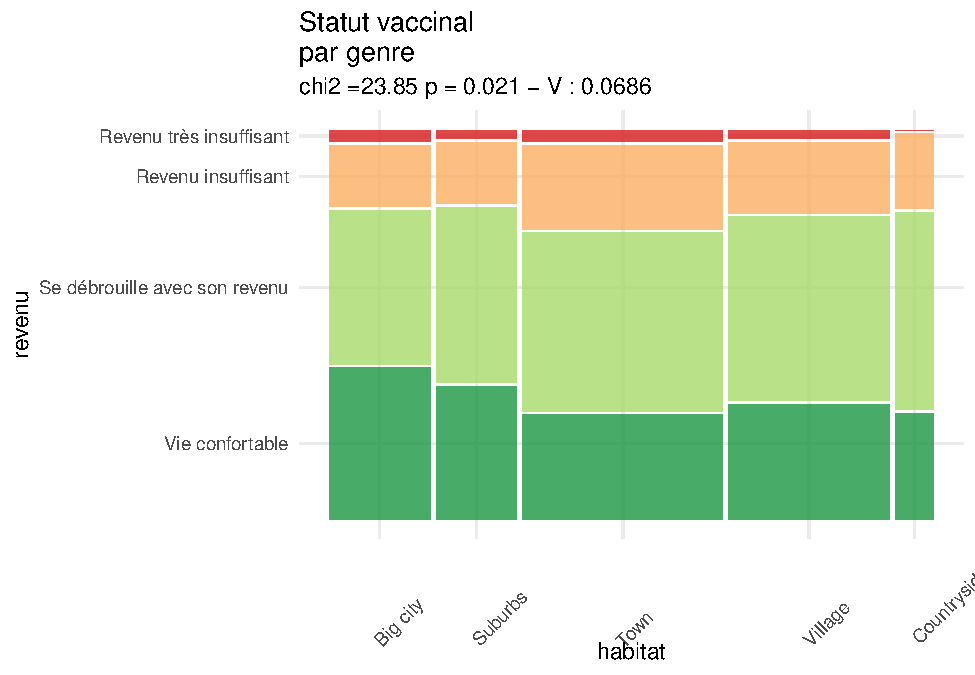
\includegraphics{bookdown-demo_files/figure-latex/0428-1.pdf}

\hypertarget{les-chi2s-partiels-et-des-cartes-de-chaleur.}{%
\subsubsection{les chi2s partiels et des cartes de chaleur.}\label{les-chi2s-partiels-et-des-cartes-de-chaleur.}}

Une carte de chaleur représente une grandeur par un gradient de couleur pour chaque cellule définie par des variable x et y.

Faisons un premier essai pour représenter les effectifs, plutôt qu'avoir un tableau de nombres on va obtenir un tableau de couleurs.

L'arbre qui apparait en ligne et en colonne correspond au résultat d'une classification hiérarchique que nous développons dans le chapitre X.

\begin{Shaded}
\begin{Highlighting}[]
\FunctionTok{library}\NormalTok{(pheatmap)}
\FunctionTok{library}\NormalTok{(viridis)}

\NormalTok{table2}\OtherTok{\textless{}{-}}\FunctionTok{as.data.frame}\NormalTok{(t) }\SpecialCharTok{\%\textgreater{}\%}
  \FunctionTok{pivot\_wider}\NormalTok{(}\AttributeTok{names\_from =}\NormalTok{ Var1, }\AttributeTok{values\_from =}\NormalTok{ Freq) }\SpecialCharTok{\%\textgreater{}\%}
  \FunctionTok{column\_to\_rownames}\NormalTok{( }\AttributeTok{var =} \StringTok{"Var2"}\NormalTok{)}
\FunctionTok{pheatmap}\NormalTok{(table2 , }\AttributeTok{color =} \FunctionTok{rocket}\NormalTok{(}\DecValTok{10}\NormalTok{,}\AttributeTok{direction =}\SpecialCharTok{{-}}\DecValTok{1}\NormalTok{))}
\end{Highlighting}
\end{Shaded}

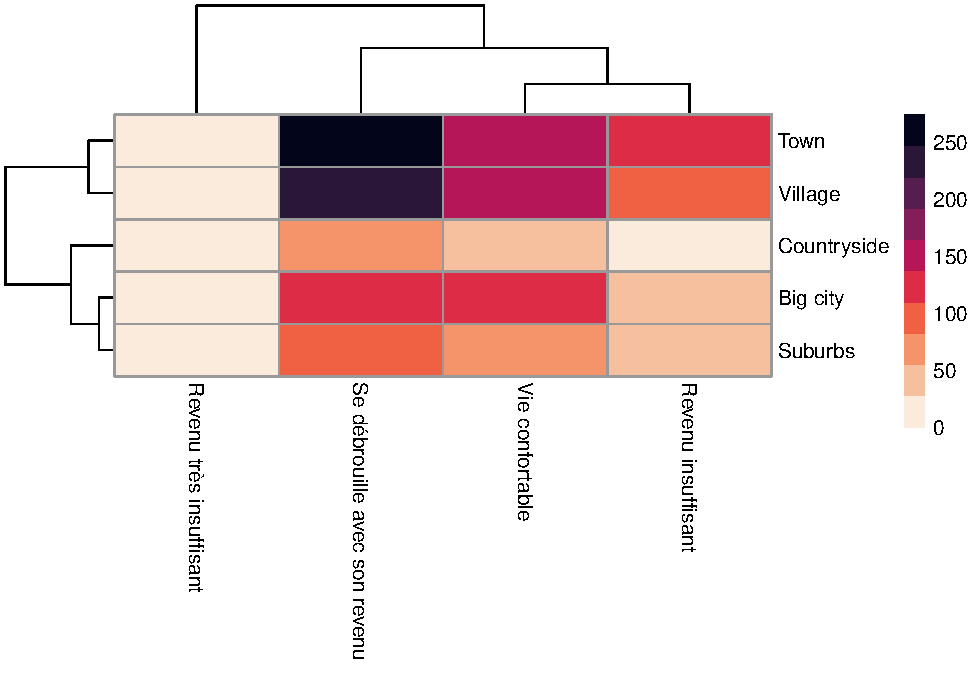
\includegraphics{bookdown-demo_files/figure-latex/0429-1.pdf}

On utilise la même technique mais en représenant une grandeur différentes : les tests du chi2 partiels, pour apprécier les sous ou les sur-représentation.

\begin{Shaded}
\begin{Highlighting}[]
\NormalTok{chi2df}\OtherTok{\textless{}{-}} \FunctionTok{as.data.frame}\NormalTok{(chi2}\SpecialCharTok{$}\NormalTok{stdres)}

\NormalTok{table2}\OtherTok{\textless{}{-}}\NormalTok{chi2df }\SpecialCharTok{\%\textgreater{}\%} 
  \FunctionTok{pivot\_wider}\NormalTok{(}\AttributeTok{names\_from =}\NormalTok{ Var1, }\AttributeTok{values\_from =}\NormalTok{ Freq) }\SpecialCharTok{\%\textgreater{}\%}
  \FunctionTok{column\_to\_rownames}\NormalTok{( }\AttributeTok{var =} \StringTok{"Var2"}\NormalTok{)}
\FunctionTok{pheatmap}\NormalTok{(table2 , }\AttributeTok{color =} \FunctionTok{brewer.pal}\NormalTok{(}\AttributeTok{n =} \DecValTok{9}\NormalTok{, }\AttributeTok{name =} \StringTok{"RdBu"}\NormalTok{))}
\end{Highlighting}
\end{Shaded}

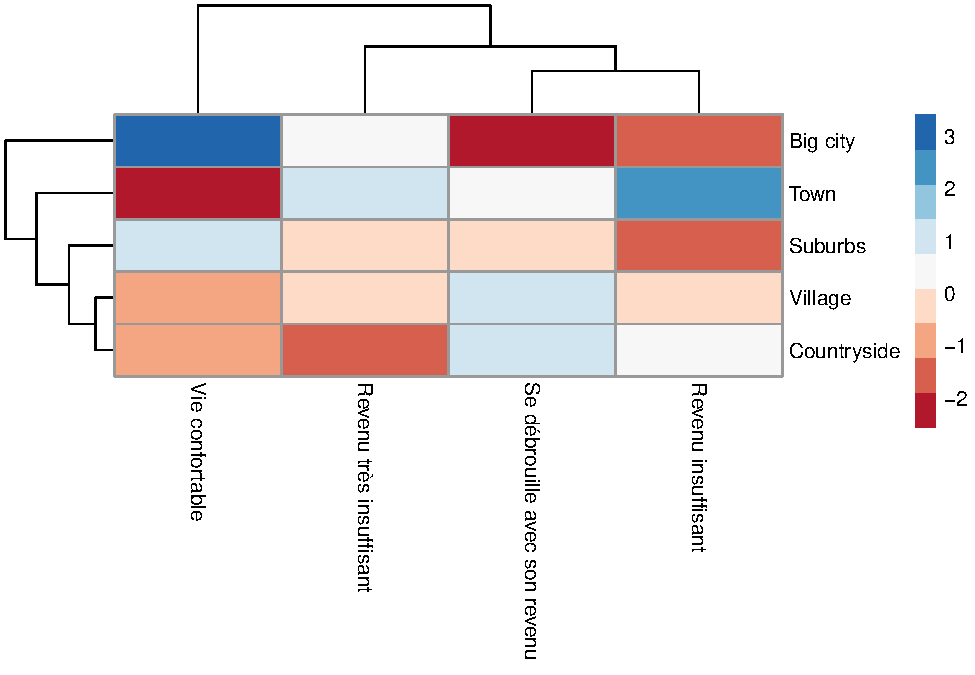
\includegraphics{bookdown-demo_files/figure-latex/0430-1.pdf}

\hypertarget{les-treemaps-cest-merveilleux}{%
\subsubsection{Les treemaps, c'est merveilleux}\label{les-treemaps-cest-merveilleux}}

D'autre graphiques et des emboîtements

\begin{Shaded}
\begin{Highlighting}[]
\FunctionTok{library}\NormalTok{(treemapify)}
\NormalTok{tree1}\OtherTok{\textless{}{-}}\NormalTok{df }\SpecialCharTok{\%\textgreater{}\%} \FunctionTok{mutate}\NormalTok{(}\AttributeTok{n=}\DecValTok{1}\NormalTok{)}\SpecialCharTok{\%\textgreater{}\%}\FunctionTok{group\_by}\NormalTok{(cntry,genre,habitat) }\SpecialCharTok{\%\textgreater{}\%} \FunctionTok{summarize}\NormalTok{(}\AttributeTok{n=}\FunctionTok{sum}\NormalTok{(n),}\AttributeTok{mean=}\FunctionTok{mean}\NormalTok{(trust\_interpersonnel, }\AttributeTok{na.rm=}\ConstantTok{TRUE}\NormalTok{))}

\NormalTok{g10 }\OtherTok{\textless{}{-}} \FunctionTok{ggplot}\NormalTok{(tree1, }\FunctionTok{aes}\NormalTok{(}\AttributeTok{area =}\NormalTok{ n, }\AttributeTok{fill=}\NormalTok{genre,}\AttributeTok{subgroup=}\NormalTok{cntry)) }\SpecialCharTok{+}
  \FunctionTok{geom\_treemap}\NormalTok{() }\SpecialCharTok{+}   
  \FunctionTok{geom\_treemap\_text}\NormalTok{(}\FunctionTok{aes}\NormalTok{(}\AttributeTok{label=}\NormalTok{habitat),}\AttributeTok{colour =} \StringTok{"white"}\NormalTok{, }\AttributeTok{place =} \StringTok{"centre"}\NormalTok{,}\AttributeTok{grow =} \ConstantTok{FALSE}\NormalTok{)}\SpecialCharTok{+}
      \FunctionTok{geom\_treemap\_subgroup\_text}\NormalTok{(}\AttributeTok{color=}\StringTok{"white"}\NormalTok{,}\AttributeTok{grow =} \ConstantTok{FALSE}\NormalTok{)}\SpecialCharTok{+}
  \FunctionTok{geom\_treemap\_subgroup\_border}\NormalTok{()}
\NormalTok{g10}
\end{Highlighting}
\end{Shaded}

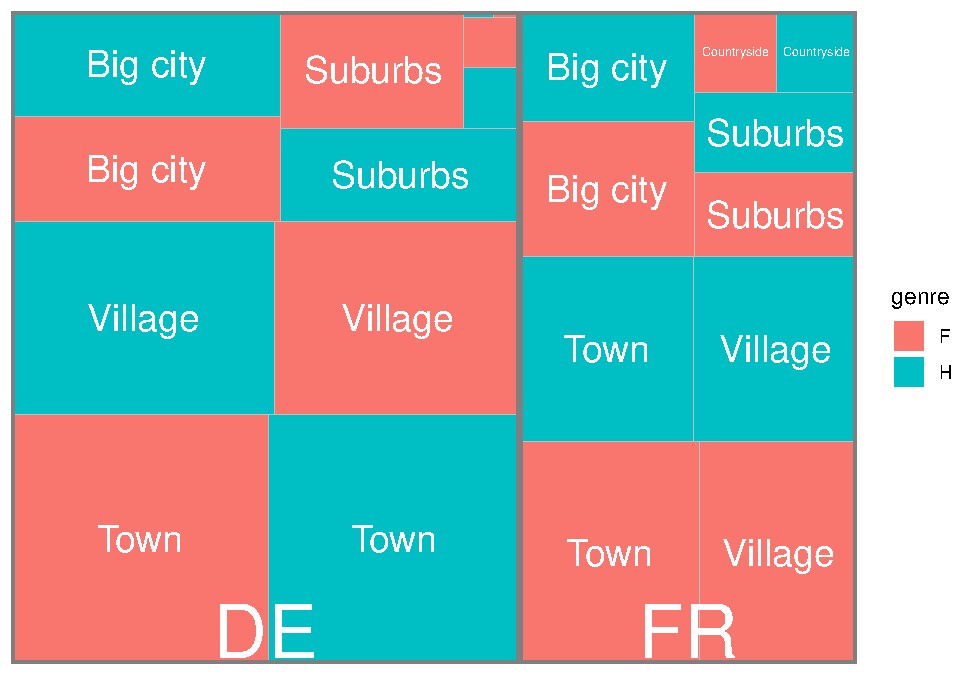
\includegraphics{bookdown-demo_files/figure-latex/0431-1.pdf}

\hypertarget{analyse-graphique-multivariuxe9e}{%
\chapter{Analyse graphique multivariée}\label{analyse-graphique-multivariuxe9e}}

Dans ce chapitre, on généralise à des ensembles de variables.

\hypertarget{la-confiance-institutionnelle-en-duxe9tail}{%
\section{La confiance institutionnelle, en détail}\label{la-confiance-institutionnelle-en-duxe9tail}}

On veut reprénter 6 variables, correspondant à 5 types d'habitats et 2 pays.

\begin{Shaded}
\begin{Highlighting}[]
\NormalTok{df}\OtherTok{\textless{}{-}}\FunctionTok{readRDS}\NormalTok{(}\StringTok{"./data/dfTrust.rds)"}\NormalTok{)}


\NormalTok{rad}\OtherTok{\textless{}{-}}\NormalTok{df }\SpecialCharTok{\%\textgreater{}\%} 
  \FunctionTok{group\_by}\NormalTok{ (habitat,cntry) }\SpecialCharTok{\%\textgreater{}\%} 
  \FunctionTok{summarize}\NormalTok{(}\AttributeTok{Partis=}\FunctionTok{mean}\NormalTok{(Partis, }\AttributeTok{na.rm=}\ConstantTok{TRUE}\NormalTok{),}
  \AttributeTok{Parlement=}\FunctionTok{mean}\NormalTok{(Parlement, }\AttributeTok{na.rm=}\ConstantTok{TRUE}\NormalTok{),}
  \AttributeTok{Politiques=}\FunctionTok{mean}\NormalTok{(Politiques, }\AttributeTok{na.rm=}\ConstantTok{TRUE}\NormalTok{),}
  \AttributeTok{Police=}\FunctionTok{mean}\NormalTok{(Police, }\AttributeTok{na.rm=}\ConstantTok{TRUE}\NormalTok{),}
  \AttributeTok{Justice=}\FunctionTok{mean}\NormalTok{(Justice, }\AttributeTok{na.rm=}\ConstantTok{TRUE}\NormalTok{),}
  \AttributeTok{NationsUnies=}\FunctionTok{mean}\NormalTok{(NationsUnies, }\AttributeTok{na.rm=}\ConstantTok{TRUE}\NormalTok{),}
  \AttributeTok{ParlementEurop=}\FunctionTok{mean}\NormalTok{(ParlementEurop, }\AttributeTok{na.rm=}\ConstantTok{TRUE}\NormalTok{)) }\SpecialCharTok{\%\textgreater{}\%} 
  \FunctionTok{filter}\NormalTok{(}\SpecialCharTok{!}\FunctionTok{is.na}\NormalTok{(habitat)) }\SpecialCharTok{\%\textgreater{}\%}
  \FunctionTok{gather}\NormalTok{(variable, value, }\SpecialCharTok{{-}}\NormalTok{habitat, }\SpecialCharTok{{-}}\NormalTok{cntry)}

\FunctionTok{ggplot}\NormalTok{(rad, }\FunctionTok{aes}\NormalTok{(}\AttributeTok{x=}\FunctionTok{reorder}\NormalTok{(variable, value),}\AttributeTok{y=}\NormalTok{value, }\AttributeTok{group=}\NormalTok{habitat))}\SpecialCharTok{+}
  \FunctionTok{geom\_line}\NormalTok{(}\FunctionTok{aes}\NormalTok{(}\AttributeTok{color=}\NormalTok{habitat), }\AttributeTok{size=}\DecValTok{2}\NormalTok{)}\SpecialCharTok{+}
  \FunctionTok{facet\_grid}\NormalTok{(.}\SpecialCharTok{\textasciitilde{}}\NormalTok{cntry) }\SpecialCharTok{+}\FunctionTok{coord\_flip}\NormalTok{()}\SpecialCharTok{+}
  \FunctionTok{scale\_color\_brewer}\NormalTok{(}\AttributeTok{type=}\StringTok{"div"}\NormalTok{,}\AttributeTok{palette=}\DecValTok{3}\NormalTok{)}\SpecialCharTok{+}\FunctionTok{labs}\NormalTok{(}\AttributeTok{title=} \StringTok{"Les éléments de la confiance institutionnelle"}\NormalTok{, }\AttributeTok{caption=}\StringTok{"ESS2002{-}2018"}\NormalTok{,}\AttributeTok{y=} \StringTok{"confiance (de 1 à 10)"}\NormalTok{,}\AttributeTok{x=}\StringTok{"institutions"}\NormalTok{) }
\end{Highlighting}
\end{Shaded}

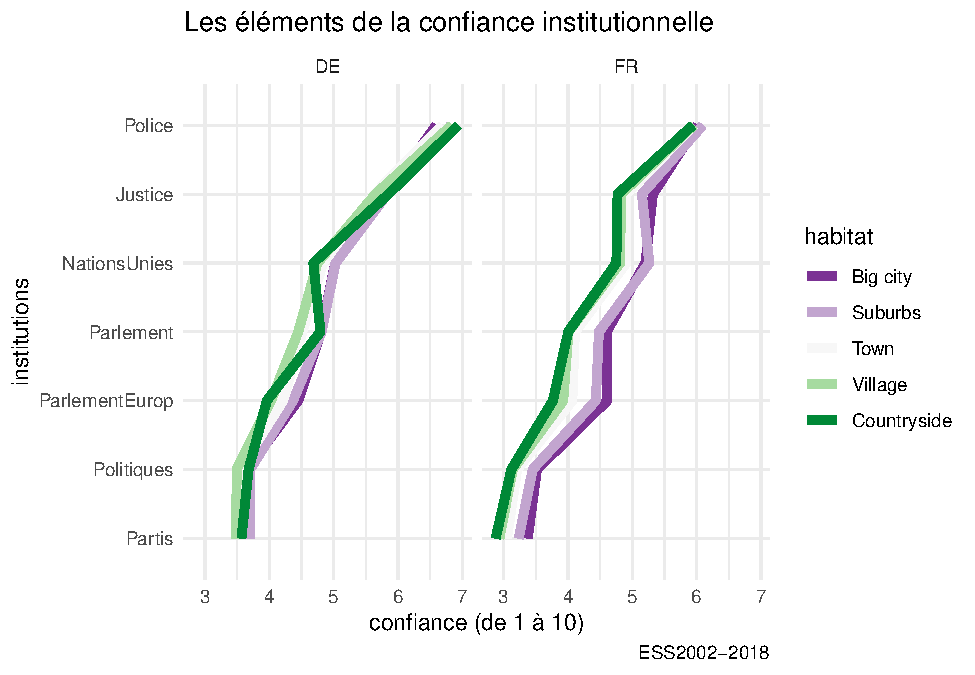
\includegraphics{bookdown-demo_files/figure-latex/0501-1.pdf}

Une autre variante qui donne l'évolution de l'évolution de les éléments de la confiance institutionnelle

\begin{Shaded}
\begin{Highlighting}[]
\NormalTok{rad}\OtherTok{\textless{}{-}}\NormalTok{df }\SpecialCharTok{\%\textgreater{}\%} 
  \FunctionTok{group\_by}\NormalTok{ (Year,cntry) }\SpecialCharTok{\%\textgreater{}\%} 
  \FunctionTok{summarize}\NormalTok{(}\AttributeTok{Partis=}\FunctionTok{mean}\NormalTok{(Partis, }\AttributeTok{na.rm=}\ConstantTok{TRUE}\NormalTok{),}
  \AttributeTok{Parlement=}\FunctionTok{mean}\NormalTok{(Parlement, }\AttributeTok{na.rm=}\ConstantTok{TRUE}\NormalTok{),}
  \AttributeTok{Politiques=}\FunctionTok{mean}\NormalTok{(Politiques, }\AttributeTok{na.rm=}\ConstantTok{TRUE}\NormalTok{),}
  \AttributeTok{Police=}\FunctionTok{mean}\NormalTok{(Police, }\AttributeTok{na.rm=}\ConstantTok{TRUE}\NormalTok{),}
  \AttributeTok{Justice=}\FunctionTok{mean}\NormalTok{(Justice, }\AttributeTok{na.rm=}\ConstantTok{TRUE}\NormalTok{),}
  \AttributeTok{NationsUnies=}\FunctionTok{mean}\NormalTok{(NationsUnies, }\AttributeTok{na.rm=}\ConstantTok{TRUE}\NormalTok{),}
  \AttributeTok{ParlementEurop=}\FunctionTok{mean}\NormalTok{(ParlementEurop, }\AttributeTok{na.rm=}\ConstantTok{TRUE}\NormalTok{)) }\SpecialCharTok{\%\textgreater{}\%} 
  \FunctionTok{gather}\NormalTok{(variable, value, }\SpecialCharTok{{-}}\NormalTok{Year, }\SpecialCharTok{{-}}\NormalTok{cntry)}

\FunctionTok{ggplot}\NormalTok{(rad, }\FunctionTok{aes}\NormalTok{(}\AttributeTok{x=}\NormalTok{Year,}\AttributeTok{y=}\NormalTok{value, }\AttributeTok{group=}\NormalTok{variable))}\SpecialCharTok{+}
  \FunctionTok{geom\_line}\NormalTok{(}\FunctionTok{aes}\NormalTok{(}\AttributeTok{color=}\NormalTok{variable), }\AttributeTok{size=}\FloatTok{1.2}\NormalTok{)}\SpecialCharTok{+}
  \FunctionTok{facet\_wrap}\NormalTok{(.}\SpecialCharTok{\textasciitilde{}}\NormalTok{cntry, }\AttributeTok{nrow=}\DecValTok{1}\NormalTok{) }\SpecialCharTok{+}
  \FunctionTok{scale\_color\_brewer}\NormalTok{(}\AttributeTok{palette=}\StringTok{"Spectral"}\NormalTok{)}\SpecialCharTok{+}\FunctionTok{labs}\NormalTok{(}\AttributeTok{title=} \StringTok{"Les éléments de la confiance institutionnelle"}\NormalTok{, }\AttributeTok{caption=}\StringTok{"ESS2002{-}2018"}\NormalTok{,}\AttributeTok{y=} \StringTok{"confiance (de 1 à 10)"}\NormalTok{,}\AttributeTok{x=}\StringTok{"institutions"}\NormalTok{) }
\end{Highlighting}
\end{Shaded}

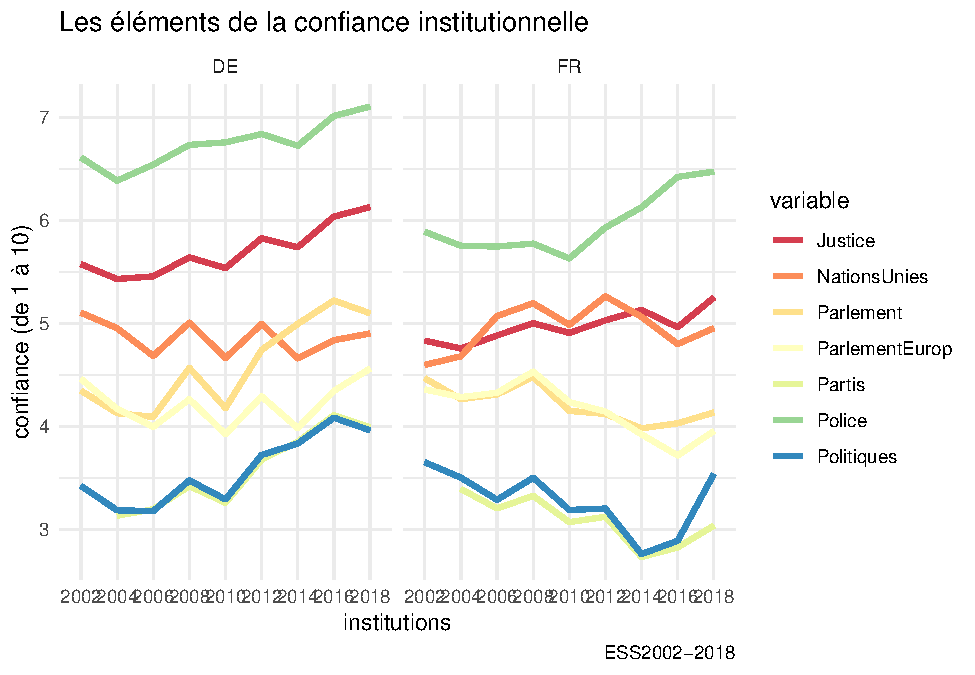
\includegraphics{bookdown-demo_files/figure-latex/0503-1.pdf}

La différence entre les deux pays est claire, la rupture est accusée plus fortement en France qu'en Allemagne. L'explication n'est sans doute pas culturelle mais démographique, un coup d'oeil à la carte des densité permet de comprendre mieux : \url{https://www.populationdata.net/cartes/allemagne-france-densite-de-population-2011/}.

On pourra tenté un graphe en radar. Mais il n'est pas si convaincant.

\begin{Shaded}
\begin{Highlighting}[]
\FunctionTok{library}\NormalTok{(fmsb)}

\NormalTok{rad}\OtherTok{\textless{}{-}}\NormalTok{df }\SpecialCharTok{\%\textgreater{}\%} \FunctionTok{filter}\NormalTok{(cntry}\SpecialCharTok{==}\StringTok{"FR"}\NormalTok{) }\SpecialCharTok{\%\textgreater{}\%}
  \FunctionTok{group\_by}\NormalTok{ (habitat) }\SpecialCharTok{\%\textgreater{}\%}
  \FunctionTok{summarize}\NormalTok{(}\AttributeTok{Partis=}\FunctionTok{mean}\NormalTok{(Partis, }\AttributeTok{na.rm=}\ConstantTok{TRUE}\NormalTok{),}
  \AttributeTok{Parlement=}\FunctionTok{mean}\NormalTok{(Parlement, }\AttributeTok{na.rm=}\ConstantTok{TRUE}\NormalTok{),}
  \AttributeTok{Politiques=}\FunctionTok{mean}\NormalTok{(Politiques, }\AttributeTok{na.rm=}\ConstantTok{TRUE}\NormalTok{),}
  \AttributeTok{Police=}\FunctionTok{mean}\NormalTok{(Police, }\AttributeTok{na.rm=}\ConstantTok{TRUE}\NormalTok{),}
  \AttributeTok{Justice=}\FunctionTok{mean}\NormalTok{(Justice, }\AttributeTok{na.rm=}\ConstantTok{TRUE}\NormalTok{),}
  \AttributeTok{NationsUnies=}\FunctionTok{mean}\NormalTok{(NationsUnies, }\AttributeTok{na.rm=}\ConstantTok{TRUE}\NormalTok{),}
  \AttributeTok{ParlementEurop=}\FunctionTok{mean}\NormalTok{(ParlementEurop, }\AttributeTok{na.rm=}\ConstantTok{TRUE}\NormalTok{)) }\SpecialCharTok{\%\textgreater{}\%} 
  \FunctionTok{filter}\NormalTok{(}\SpecialCharTok{!}\FunctionTok{is.na}\NormalTok{(habitat)) }\SpecialCharTok{\%\textgreater{}\%} 
\NormalTok{  dplyr}\SpecialCharTok{::}\FunctionTok{select}\NormalTok{(}\SpecialCharTok{{-}}\NormalTok{habitat)}

\CommentTok{\#on doit indiquer les valeurs minimale et maximale {-} la fonction rep permet de repeter (ici 7 fois pour les 7 variables/col)}
\NormalTok{data }\OtherTok{\textless{}{-}} \FunctionTok{rbind}\NormalTok{(}\FunctionTok{rep}\NormalTok{(}\DecValTok{7}\NormalTok{,}\DecValTok{7}\NormalTok{) , }\FunctionTok{rep}\NormalTok{(}\DecValTok{3}\NormalTok{,}\DecValTok{7}\NormalTok{) , rad)}
\CommentTok{\#l\textquotesingle{}autre method c\textquotesingle{}est ce choisir maxmin=FALSE}

\CommentTok{\#rownames(rad) \textless{}{-} c("big city", "suburbs" ,"town","village", "countryside")}
\FunctionTok{radarchart}\NormalTok{(rad, }\AttributeTok{axistype=}\DecValTok{0}\NormalTok{, }\AttributeTok{seg=}\DecValTok{4}\NormalTok{, }\AttributeTok{title=}\StringTok{"Moyenne par institution"}\NormalTok{, }\AttributeTok{maxmin=}\ConstantTok{FALSE}\NormalTok{)}
\FunctionTok{legend}\NormalTok{(}\AttributeTok{x=}\FloatTok{0.7}\NormalTok{, }\AttributeTok{y=}\DecValTok{1}\NormalTok{, }\AttributeTok{legend =} \FunctionTok{rownames}\NormalTok{(rad), }\AttributeTok{bty =} \StringTok{"n"}\NormalTok{,}\AttributeTok{text.col =} \StringTok{"grey"}\NormalTok{, }\AttributeTok{cex=}\FloatTok{1.2}\NormalTok{, }\AttributeTok{pt.cex=}\DecValTok{3}\NormalTok{)}
\end{Highlighting}
\end{Shaded}

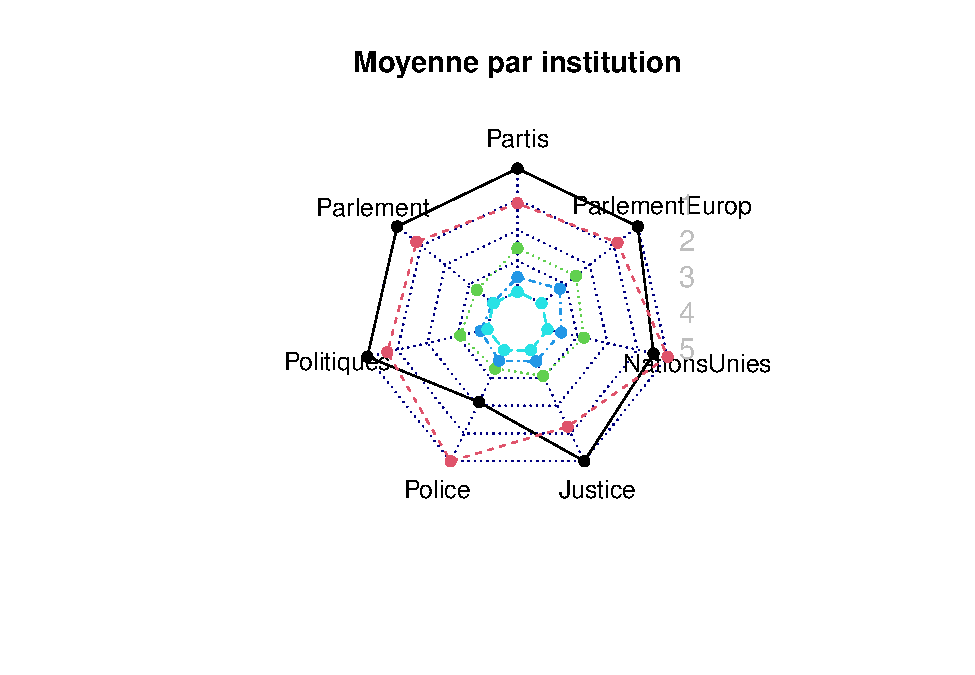
\includegraphics{bookdown-demo_files/figure-latex/0504-1.pdf}

\hypertarget{table-de-corruxe9lation}{%
\section{Table de corrélation}\label{table-de-corruxe9lation}}

Comparer les moyennes est une chose, on souhaiter en plus savoir quelle structure de corrélation les caractérisent. Rien de plus simple

\begin{Shaded}
\begin{Highlighting}[]
\FunctionTok{library}\NormalTok{(ggcorrplot)}
\NormalTok{df}\OtherTok{\textless{}{-}}\FunctionTok{readRDS}\NormalTok{(}\StringTok{"./data/dfTrust.rds)"}\NormalTok{)}\SpecialCharTok{\%\textgreater{}\%}\FunctionTok{filter}\NormalTok{(Year}\SpecialCharTok{==}\DecValTok{2018}\NormalTok{)}

\NormalTok{foo}\OtherTok{\textless{}{-}}\NormalTok{df }\SpecialCharTok{\%\textgreater{}\%}\NormalTok{ dplyr}\SpecialCharTok{::}\FunctionTok{select}\NormalTok{(NationsUnies,ParlementEurop, Parlement, Justice, Police, Politiques, Partis) }\SpecialCharTok{\%\textgreater{}\%} 
  \FunctionTok{drop\_na}\NormalTok{()}
\NormalTok{r}\OtherTok{\textless{}{-}}\FunctionTok{cor}\NormalTok{(foo)}

\FunctionTok{ggcorrplot}\NormalTok{(r, }\AttributeTok{hc.order =} \ConstantTok{TRUE}\NormalTok{, }\AttributeTok{type =} \StringTok{"lower"}\NormalTok{,}
   \AttributeTok{lab =} \ConstantTok{TRUE}\NormalTok{)}
\end{Highlighting}
\end{Shaded}

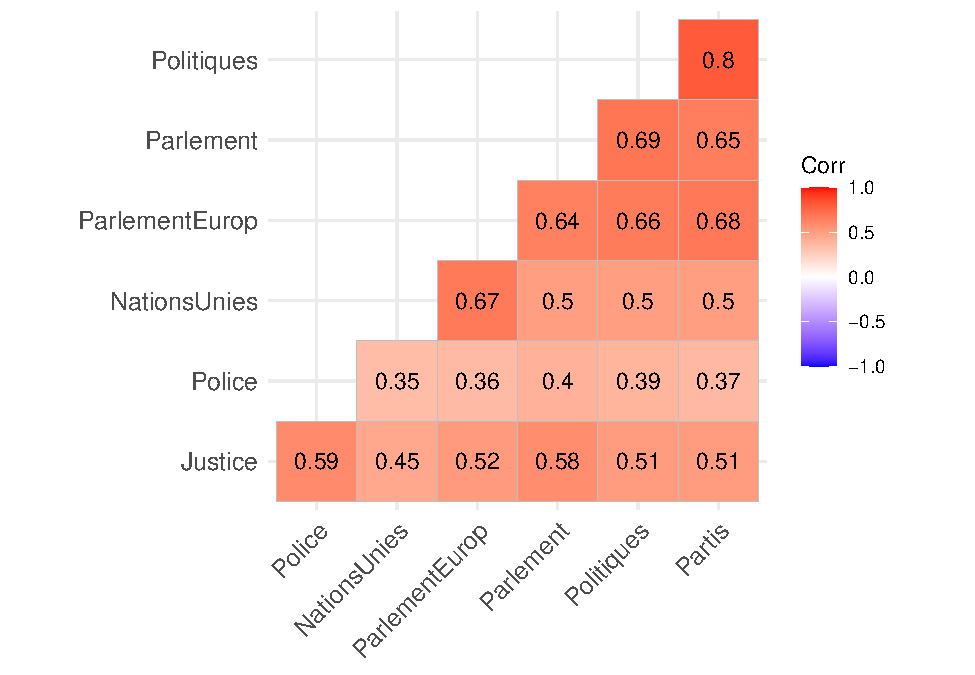
\includegraphics{bookdown-demo_files/figure-latex/0505-1.pdf}

\begin{Shaded}
\begin{Highlighting}[]
\NormalTok{g}\OtherTok{\textless{}{-}}\FunctionTok{paste0}\NormalTok{(}\StringTok{"./plot/g1"}\NormalTok{,}\StringTok{".jpg"}\NormalTok{)}
\FunctionTok{ggsave}\NormalTok{(g,}\AttributeTok{plot=}\FunctionTok{last\_plot}\NormalTok{(), }\AttributeTok{width =} \DecValTok{27}\NormalTok{, }\AttributeTok{height =} \DecValTok{19}\NormalTok{, }\AttributeTok{units =} \StringTok{"cm"}\NormalTok{)}
\end{Highlighting}
\end{Shaded}

\hypertarget{un-cas-plus-complexe-pruxe9sidentielle2020}{%
\section{Un cas plus complexe : présidentielle2020}\label{un-cas-plus-complexe-pruxe9sidentielle2020}}

Nsppolls cumulent les sondages publiés des grands instituts. On utilise ces données , ainsi qu'une boucle, pour explorer différents paramètre d'un modèle de lissage.

Le but : mieux percevoir les tendance par une sorte de méta-analyse des différents sondages :

\hypertarget{une-boucle-pour-produire-de-multiple-graphe-en-variant-un-paramuxe8tre}{%
\section{une boucle pour produire de multiple graphe en variant un paramètre}\label{une-boucle-pour-produire-de-multiple-graphe-en-variant-un-paramuxe8tre}}

\begin{Shaded}
\begin{Highlighting}[]
\FunctionTok{library}\NormalTok{(lubridate)}
\NormalTok{alph}\OtherTok{\textless{}{-}}\NormalTok{.}\DecValTok{5}

\ControlFlowTok{for}\NormalTok{ (alph }\ControlFlowTok{in} \FunctionTok{seq}\NormalTok{(}\AttributeTok{from=}\DecValTok{0}\NormalTok{, }\AttributeTok{to=} \DecValTok{1}\NormalTok{, }\AttributeTok{by=}\NormalTok{.}\DecValTok{05}\NormalTok{))\{}
\NormalTok{df\_pol }\OtherTok{\textless{}{-}} \FunctionTok{read\_delim}\NormalTok{(}\StringTok{"https://raw.githubusercontent.com/nsppolls/nsppolls/master/presidentielle.csv"}\NormalTok{, }
                     \AttributeTok{delim =} \StringTok{","}\NormalTok{, }\AttributeTok{escape\_double =} \ConstantTok{FALSE}\NormalTok{, }\AttributeTok{trim\_ws =} \ConstantTok{TRUE}\NormalTok{)}\SpecialCharTok{\%\textgreater{}\%}
  \FunctionTok{filter}\NormalTok{(tour}\SpecialCharTok{==}\StringTok{"Premier tour"}\NormalTok{) }\SpecialCharTok{\%\textgreater{}\%}\FunctionTok{filter}\NormalTok{(candidat}\SpecialCharTok{==}\StringTok{"Eric Zemmour"}\SpecialCharTok{|}
\NormalTok{                                           candidat}\SpecialCharTok{==} \StringTok{"Marine Le Pen"}\SpecialCharTok{|}
\NormalTok{                                           candidat}\SpecialCharTok{==} \StringTok{"Emmanuel Macron"}\SpecialCharTok{|}
\NormalTok{                                           candidat}\SpecialCharTok{==} \StringTok{"Jean{-}Luc Mélenchon"}\SpecialCharTok{|}
\NormalTok{                                           candidat}\SpecialCharTok{==} \StringTok{"Yannick Jadot"}\SpecialCharTok{|}
\NormalTok{                                           candidat}\SpecialCharTok{==} \StringTok{"Valérie Pécresse"}\SpecialCharTok{|} 
\NormalTok{                                           candidat}\SpecialCharTok{==}\StringTok{"Fabien Roussel"}\SpecialCharTok{|}
\NormalTok{                                           candidat}\SpecialCharTok{==}\StringTok{"Anne Hidalgo"}\NormalTok{) }\SpecialCharTok{\%\textgreater{}\%}
  \FunctionTok{filter}\NormalTok{(fin\_enquete}\SpecialCharTok{\textgreater{}}\FunctionTok{ymd}\NormalTok{(}\StringTok{"2022{-}01{-}09"}\NormalTok{)) }\CommentTok{\# on commence en septembre , octobre est{-}il meilleur ?}


\FunctionTok{table}\NormalTok{(df\_pol}\SpecialCharTok{$}\NormalTok{candidat)}
\NormalTok{SensiP1}\OtherTok{\textless{}{-}}\FunctionTok{c}\NormalTok{(}\StringTok{"pink"}\NormalTok{, }\StringTok{"orange"}\NormalTok{, }\StringTok{"gray20"}\NormalTok{, }\StringTok{"red"}\NormalTok{,}\StringTok{"firebrick"}\NormalTok{, }\StringTok{"Royalblue"}\NormalTok{, }\StringTok{" skyblue"}\NormalTok{, }\StringTok{"Chartreuse"}\NormalTok{)}

\FunctionTok{ggplot}\NormalTok{(df\_pol, }\FunctionTok{aes}\NormalTok{(}\AttributeTok{y=}\NormalTok{intentions, }\AttributeTok{x=}\NormalTok{fin\_enquete))}\SpecialCharTok{+}
  \FunctionTok{geom\_point}\NormalTok{(}\FunctionTok{aes}\NormalTok{(}\AttributeTok{color=}\NormalTok{candidat), }\AttributeTok{size=}\NormalTok{.}\DecValTok{5}\NormalTok{, }\AttributeTok{alpha=}\DecValTok{1}\SpecialCharTok{{-}}\NormalTok{alph)}\SpecialCharTok{+}
  \FunctionTok{geom\_smooth}\NormalTok{(}\AttributeTok{span =}\NormalTok{ alph, }\FunctionTok{aes}\NormalTok{(}\AttributeTok{col=}\NormalTok{candidat,}\AttributeTok{fill=}\NormalTok{candidat), }\AttributeTok{alpha=}\FloatTok{0.2}\NormalTok{)}\SpecialCharTok{+}
  \FunctionTok{scale\_color\_manual}\NormalTok{(}\AttributeTok{values=}\NormalTok{SensiP1)}\SpecialCharTok{+}  
  \FunctionTok{scale\_fill\_manual}\NormalTok{(}\AttributeTok{values=}\NormalTok{SensiP1)}\SpecialCharTok{+} 
  \FunctionTok{labs}\NormalTok{(}\AttributeTok{title=} \StringTok{"Evolution des intentions de vote \#présidentielle2022 1er tour"}\NormalTok{,}
       \AttributeTok{subtitle =}\FunctionTok{paste}\NormalTok{(}\StringTok{"Lissage méthode loess. alpha="}\NormalTok{,alph, }\StringTok{" {-} ci=95\%"}\NormalTok{),}
       \AttributeTok{caption =} \StringTok{"data @nsppolls viz @benavent"}\NormalTok{,}
       \AttributeTok{x=}\ConstantTok{NULL}\NormalTok{)}\SpecialCharTok{+}\FunctionTok{theme\_minimal}\NormalTok{()}\SpecialCharTok{+}\FunctionTok{scale\_x\_date}\NormalTok{(}\AttributeTok{date\_breaks =} \StringTok{"1 month"}\NormalTok{, }\AttributeTok{date\_minor\_breaks =} \StringTok{"1 week"}\NormalTok{,}
             \AttributeTok{date\_labels =} \StringTok{"\%B"}\NormalTok{)}

\NormalTok{sondage\_nsppolls}\OtherTok{\textless{}{-}}\FunctionTok{paste0}\NormalTok{(}\StringTok{"./nsppolls/sondage\_nsppolls"}\NormalTok{, alph}\SpecialCharTok{*}\DecValTok{20}\NormalTok{, }\StringTok{".jpg"}\NormalTok{)}
\FunctionTok{ggsave}\NormalTok{(sondage\_nsppolls,}\AttributeTok{plot=}\FunctionTok{last\_plot}\NormalTok{(), }\AttributeTok{width =} \DecValTok{27}\NormalTok{, }\AttributeTok{height =} \DecValTok{19}\NormalTok{, }\AttributeTok{units =} \StringTok{"cm"}\NormalTok{)}

\NormalTok{\}}


\NormalTok{n}\OtherTok{\textless{}{-}}\NormalTok{df\_pol}\SpecialCharTok{\%\textgreater{}\%}
  \FunctionTok{mutate}\NormalTok{(}\AttributeTok{n=}\DecValTok{1}\NormalTok{)}\SpecialCharTok{\%\textgreater{}\%}
  \FunctionTok{group\_by}\NormalTok{(id)}\SpecialCharTok{\%\textgreater{}\%}\FunctionTok{summarise}\NormalTok{(}\AttributeTok{n=}\FunctionTok{sum}\NormalTok{(n))}
\CommentTok{\#nombre de sondage}
\NormalTok{n}\OtherTok{\textless{}{-}}\FunctionTok{nrow}\NormalTok{(n)}
\end{Highlighting}
\end{Shaded}

Pour créer le gif on emplie magick. On a pris soin de sauvegarder les graphes dans un répertoire propre, ça facilite la lecture en boucle et la fabrication du gif.

\begin{Shaded}
\begin{Highlighting}[]
\FunctionTok{library}\NormalTok{(magick)}

\CommentTok{\#gif                                                     }

\CommentTok{\#on constitue une liste des noms des fichier *.jpg que l\textquotesingle{}on veut associer                                                     }
\NormalTok{frames }\OtherTok{\textless{}{-}} \FunctionTok{paste0}\NormalTok{(}\StringTok{"./nsppolls/"}\NormalTok{,}\StringTok{"sondage\_nsppolls"}\NormalTok{, }\DecValTok{0}\SpecialCharTok{:}\DecValTok{20}\NormalTok{,}\StringTok{".jpg"}\NormalTok{)}

\CommentTok{\#on lit et on stoke dans m les images}
\NormalTok{m }\OtherTok{\textless{}{-}} \FunctionTok{image\_read}\NormalTok{(frames)}

\CommentTok{\#on fabrique et on sauvergarde le gif}
\NormalTok{m }\OtherTok{\textless{}{-}} \FunctionTok{image\_animate}\NormalTok{(m, }\AttributeTok{fps=}\DecValTok{1}\NormalTok{)}
\FunctionTok{image\_write}\NormalTok{(m, }\StringTok{"./plot/sondages\_lissage.gif"}\NormalTok{)}
\end{Highlighting}
\end{Shaded}

\hypertarget{effet-sondeur}{%
\subsection{effet sondeur}\label{effet-sondeur}}

pour anticiper sur le chapitre suivant

\begin{Shaded}
\begin{Highlighting}[]
\NormalTok{foo}\OtherTok{\textless{}{-}}\NormalTok{df\_pol}\SpecialCharTok{\%\textgreater{}\%}
\NormalTok{  dplyr}\SpecialCharTok{::}\FunctionTok{select}\NormalTok{(candidat, intentions, fin\_enquete, echantillon,nom\_institut)}\SpecialCharTok{\%\textgreater{}\%}
  \FunctionTok{group\_by}\NormalTok{(nom\_institut, candidat)}\SpecialCharTok{\%\textgreater{}\%}
  \FunctionTok{summarise}\NormalTok{(}\AttributeTok{moy=}\FunctionTok{mean}\NormalTok{(intentions, }\AttributeTok{na.rm=}\ConstantTok{TRUE}\NormalTok{),}
            \AttributeTok{std=}\FunctionTok{sd}\NormalTok{(intentions, }\AttributeTok{na.rm=}\ConstantTok{TRUE}\NormalTok{))}


\NormalTok{SensiP2}\OtherTok{\textless{}{-}}\FunctionTok{c}\NormalTok{(}\StringTok{"gray90"}\NormalTok{,}\StringTok{"gray20"}\NormalTok{, }\StringTok{"Royalblue"}\NormalTok{, }\StringTok{"skyblue"}\NormalTok{, }\StringTok{"orange"}\NormalTok{, }\StringTok{"yellow"}\NormalTok{, }\StringTok{"pink"}\NormalTok{, }\StringTok{"firebrick"}\NormalTok{, }\StringTok{"green"}\NormalTok{, }\StringTok{"gold1"}\NormalTok{, }\StringTok{"gold2"}\NormalTok{)}


\NormalTok{g}\OtherTok{\textless{}{-}}\FunctionTok{ggplot}\NormalTok{(foo,}\FunctionTok{aes}\NormalTok{(}\AttributeTok{x=}\NormalTok{candidat,}\AttributeTok{y=}\NormalTok{moy))}\SpecialCharTok{+}
  \FunctionTok{geom\_segment}\NormalTok{(}\FunctionTok{aes}\NormalTok{(}\AttributeTok{x =}\NormalTok{ candidat, }
                   \AttributeTok{y =} \SpecialCharTok{{-}}\NormalTok{std}\SpecialCharTok{+}\NormalTok{moy, }
                   \AttributeTok{xend =}\NormalTok{ candidat, }
                   \AttributeTok{yend =}\NormalTok{ std}\SpecialCharTok{+}\NormalTok{moy, }
                   \AttributeTok{color =}\NormalTok{ nom\_institut), }\AttributeTok{size=}\FloatTok{1.2}\NormalTok{)}\SpecialCharTok{+}
    \FunctionTok{geom\_point}\NormalTok{(}\FunctionTok{aes}\NormalTok{(}\AttributeTok{color=}\NormalTok{nom\_institut), }\AttributeTok{size=}\DecValTok{2}\NormalTok{)}\SpecialCharTok{+}
  \FunctionTok{scale\_color\_manual}\NormalTok{(}\AttributeTok{values =}\NormalTok{ SensiP2)}\SpecialCharTok{+}
  \FunctionTok{theme\_minimal}\NormalTok{()}\SpecialCharTok{+}
  \FunctionTok{coord\_flip}\NormalTok{()}
\NormalTok{g}
\end{Highlighting}
\end{Shaded}

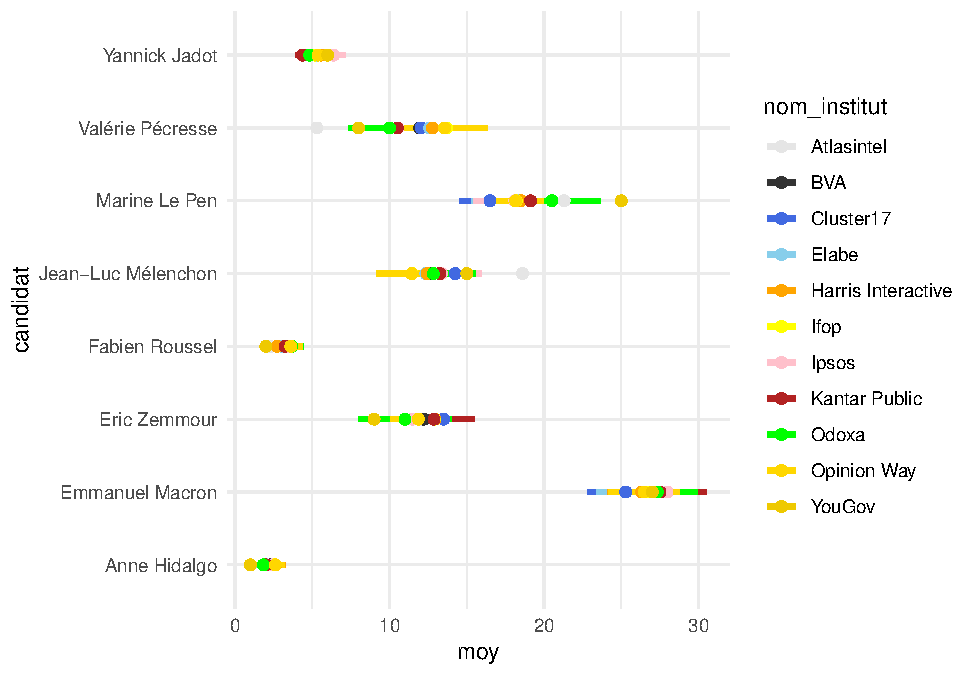
\includegraphics{bookdown-demo_files/figure-latex/0510-1.pdf}

\hypertarget{moduxe9liser-le-biais-du-sondeur}{%
\section{Modéliser le biais du sondeur}\label{moduxe9liser-le-biais-du-sondeur}}

\url{http://www.stat.yale.edu/Courses/1997-98/101/anovareg.htm}

\begin{Shaded}
\begin{Highlighting}[]
\NormalTok{df\_pol}\SpecialCharTok{$}\NormalTok{tps}\OtherTok{\textless{}{-}}\DecValTok{2}
\NormalTok{df\_pol}\SpecialCharTok{$}\NormalTok{tps[df\_pol}\SpecialCharTok{$}\NormalTok{fin\_enquete }\SpecialCharTok{\textless{}} \FunctionTok{ymd}\NormalTok{(}\StringTok{"2022{-}01{-}31"}\NormalTok{)]}\OtherTok{\textless{}{-}}\DecValTok{1}

\NormalTok{df\_pol}\SpecialCharTok{$}\NormalTok{tps[df\_pol}\SpecialCharTok{$}\NormalTok{fin\_enquete }\SpecialCharTok{\textgreater{}} \FunctionTok{ymd}\NormalTok{(}\StringTok{"2022{-}03{-}01"}\NormalTok{)]}\OtherTok{\textless{}{-}}\DecValTok{3}

\NormalTok{df\_pol}\SpecialCharTok{$}\NormalTok{tps}\OtherTok{\textless{}{-}} \FunctionTok{as.factor}\NormalTok{(df\_pol}\SpecialCharTok{$}\NormalTok{tps)}

\NormalTok{fit1}\OtherTok{\textless{}{-}} \FunctionTok{lm}\NormalTok{(intentions}\SpecialCharTok{\textasciitilde{}}\NormalTok{candidat}\SpecialCharTok{*}\NormalTok{tps,}\AttributeTok{data=}\NormalTok{df\_pol)}
\FunctionTok{anova}\NormalTok{(fit1)}
\end{Highlighting}
\end{Shaded}

\begin{verbatim}
## Analysis of Variance Table
## 
## Response: intentions
##                Df Sum Sq Mean Sq    F value    Pr(>F)    
## candidat        7 122735 17533.6 10705.9435 < 2.2e-16 ***
## tps             2     25    12.7     7.7658 0.0004363 ***
## candidat:tps   14   4534   323.9   197.7554 < 2.2e-16 ***
## Residuals    2096   3433     1.6                         
## ---
## Signif. codes:  0 '***' 0.001 '**' 0.01 '*' 0.05 '.' 0.1 ' ' 1
\end{verbatim}

\begin{Shaded}
\begin{Highlighting}[]
\NormalTok{fit2}\OtherTok{\textless{}{-}} \FunctionTok{lm}\NormalTok{(intentions}\SpecialCharTok{\textasciitilde{}}\NormalTok{candidat}\SpecialCharTok{*}\NormalTok{tps}\SpecialCharTok{+}\NormalTok{candidat}\SpecialCharTok{*}\NormalTok{nom\_institut,}\AttributeTok{data=}\NormalTok{df\_pol)}
\FunctionTok{anova}\NormalTok{(fit2)}
\end{Highlighting}
\end{Shaded}

\begin{verbatim}
## Analysis of Variance Table
## 
## Response: intentions
##                         Df Sum Sq Mean Sq    F value    Pr(>F)    
## candidat                 7 122735 17533.6 12742.2074 < 2.2e-16 ***
## tps                      2     25    12.7     9.2428  0.000101 ***
## nom_institut            10     25     2.5     1.8283  0.051096 .  
## candidat:tps            14   4534   323.9   235.3684 < 2.2e-16 ***
## candidat:nom_institut   70    633     9.0     6.5768 < 2.2e-16 ***
## Residuals             2016   2774     1.4                         
## ---
## Signif. codes:  0 '***' 0.001 '**' 0.01 '*' 0.05 '.' 0.1 ' ' 1
\end{verbatim}

\begin{Shaded}
\begin{Highlighting}[]
\FunctionTok{anova}\NormalTok{(fit1,fit2)}
\end{Highlighting}
\end{Shaded}

\begin{verbatim}
## Analysis of Variance Table
## 
## Model 1: intentions ~ candidat * tps
## Model 2: intentions ~ candidat * tps + candidat * nom_institut
##   Res.Df    RSS Df Sum of Sq      F    Pr(>F)    
## 1   2096 3432.7                                  
## 2   2016 2774.1 80    658.65 5.9832 < 2.2e-16 ***
## ---
## Signif. codes:  0 '***' 0.001 '**' 0.01 '*' 0.05 '.' 0.1 ' ' 1
\end{verbatim}

\begin{Shaded}
\begin{Highlighting}[]
\FunctionTok{summary}\NormalTok{(fit1)}
\end{Highlighting}
\end{Shaded}

\begin{verbatim}
## 
## Call:
## lm(formula = intentions ~ candidat * tps, data = df_pol)
## 
## Residuals:
##     Min      1Q  Median      3Q     Max 
## -5.2585 -0.6350 -0.0278  0.6021  5.6493 
## 
## Coefficients:
##                                 Estimate Std. Error t value Pr(>|t|)    
## (Intercept)                       3.1765     0.1792  17.726  < 2e-16 ***
## candidatEmmanuel Macron          21.5392     0.2534  84.992  < 2e-16 ***
## candidatEric Zemmour              9.7549     0.2534  38.492  < 2e-16 ***
## candidatFabien Roussel           -0.8039     0.2534  -3.172 0.001535 ** 
## candidatJean-Luc Mélenchon        6.4118     0.2534  25.300  < 2e-16 ***
## candidatMarine Le Pen            13.7353     0.2534  54.198  < 2e-16 ***
## candidatValérie Pécresse         13.2255     0.2534  52.187  < 2e-16 ***
## candidatYannick Jadot             2.7255     0.2534  10.755  < 2e-16 ***
## tps2                             -0.6765     0.2342  -2.888 0.003915 ** 
## tps3                             -0.9765     0.2089  -4.674 3.14e-06 ***
## candidatEmmanuel Macron:tps2      0.6844     0.3312   2.066 0.038934 *  
## candidatEric Zemmour:tps2         2.0645     0.3312   6.233 5.52e-10 ***
## candidatFabien Roussel:tps2       2.1511     0.3312   6.494 1.04e-10 ***
## candidatJean-Luc Mélenchon:tps2   1.6438     0.3312   4.963 7.52e-07 ***
## candidatMarine Le Pen:tps2        0.5842     0.3312   1.764 0.077955 .  
## candidatValérie Pécresse:tps2    -0.9616     0.3312  -2.903 0.003734 ** 
## candidatYannick Jadot:tps2       -0.1630     0.3312  -0.492 0.622725    
## candidatEmmanuel Macron:tps3      4.6819     0.2955  15.847  < 2e-16 ***
## candidatEric Zemmour:tps3        -1.0570     0.2955  -3.578 0.000355 ***
## candidatFabien Roussel:tps3       2.0919     0.2955   7.080 1.95e-12 ***
## candidatJean-Luc Mélenchon:tps3   5.1319     0.2955  17.370  < 2e-16 ***
## candidatMarine Le Pen:tps3        3.4154     0.2955  11.560  < 2e-16 ***
## candidatValérie Pécresse:tps3    -4.8670     0.2955 -16.473  < 2e-16 ***
## candidatYannick Jadot:tps3        0.4724     0.2955   1.599 0.109995    
## ---
## Signif. codes:  0 '***' 0.001 '**' 0.01 '*' 0.05 '.' 0.1 ' ' 1
## 
## Residual standard error: 1.28 on 2096 degrees of freedom
## Multiple R-squared:  0.9737, Adjusted R-squared:  0.9735 
## F-statistic:  3379 on 23 and 2096 DF,  p-value: < 2.2e-16
\end{verbatim}

\begin{Shaded}
\begin{Highlighting}[]
\FunctionTok{summary}\NormalTok{(fit2)}
\end{Highlighting}
\end{Shaded}

\begin{verbatim}
## 
## Call:
## lm(formula = intentions ~ candidat * tps + candidat * nom_institut, 
##     data = df_pol)
## 
## Residuals:
##     Min      1Q  Median      3Q     Max 
## -4.7981 -0.5456 -0.0272  0.5924  5.2019 
## 
## Coefficients:
##                                                           Estimate Std. Error
## (Intercept)                                                3.39409    1.18971
## candidatEmmanuel Macron                                   20.60082    1.68251
## candidatEric Zemmour                                      10.59844    1.68251
## candidatFabien Roussel                                    -2.19508    1.68251
## candidatJean-Luc Mélenchon                                11.04593    1.68251
## candidatMarine Le Pen                                     15.30968    1.68251
## candidatValérie Pécresse                                   7.55835    1.68251
## candidatYannick Jadot                                      2.30826    1.68251
## tps2                                                      -0.68106    0.21565
## tps3                                                      -0.99409    0.19847
## nom_institutBVA                                           -0.30224    1.23753
## nom_institutCluster17                                     -0.84531    1.21657
## nom_institutElabe                                         -0.71509    1.21215
## nom_institutHarris Interactive                            -0.18347    1.21291
## nom_institutIfop                                          -0.18249    1.18474
## nom_institutIpsos                                         -0.08904    1.19038
## nom_institutKantar Public                                 -0.47826    1.31223
## nom_institutOdoxa                                         -0.67101    1.35576
## nom_institutOpinion Way                                   -0.04925    1.18126
## nom_institutYouGov                                        -1.40000    1.65893
## candidatEmmanuel Macron:tps2                               0.73921    0.30498
## candidatEric Zemmour:tps2                                  2.12294    0.30498
## candidatFabien Roussel:tps2                                2.12788    0.30498
## candidatJean-Luc Mélenchon:tps2                            1.71555    0.30498
## candidatMarine Le Pen:tps2                                 0.60025    0.30498
## candidatValérie Pécresse:tps2                             -0.97779    0.30498
## candidatYannick Jadot:tps2                                -0.15932    0.30498
## candidatEmmanuel Macron:tps3                               4.79918    0.28068
## candidatEric Zemmour:tps3                                 -0.99844    0.28068
## candidatFabien Roussel:tps3                                2.09508    0.28068
## candidatJean-Luc Mélenchon:tps3                            5.15407    0.28068
## candidatMarine Le Pen:tps3                                 3.59032    0.28068
## candidatValérie Pécresse:tps3                             -4.65835    0.28068
## candidatYannick Jadot:tps3                                 0.29174    0.28068
## candidatEmmanuel Macron:nom_institutBVA                    0.75768    1.75014
## candidatEric Zemmour:nom_institutBVA                      -0.46013    1.75014
## candidatFabien Roussel:nom_institutBVA                     1.43661    1.75014
## candidatJean-Luc Mélenchon:nom_institutBVA                -4.47432    1.75014
## candidatMarine Le Pen:nom_institutBVA                     -1.61439    1.75014
## candidatValérie Pécresse:nom_institutBVA                   5.43117    1.75014
## candidatYannick Jadot:nom_institutBVA                      0.47709    1.75014
## candidatEmmanuel Macron:nom_institutCluster17              0.21696    1.72049
## candidatEric Zemmour:nom_institutCluster17                 0.93708    1.72049
## candidatFabien Roussel:nom_institutCluster17               1.75386    1.72049
## candidatJean-Luc Mélenchon:nom_institutCluster17          -1.72026    1.72049
## candidatMarine Le Pen:nom_institutCluster17               -2.63348    1.72049
## candidatValérie Pécresse:nom_institutCluster17             5.22876    1.72049
## candidatYannick Jadot:nom_institutCluster17                0.59139    1.72049
## candidatEmmanuel Macron:nom_institutElabe                  1.38103    1.71424
## candidatEric Zemmour:nom_institutElabe                    -1.35629    1.71424
## candidatFabien Roussel:nom_institutElabe                   1.64477    1.71424
## candidatJean-Luc Mélenchon:nom_institutElabe              -3.52444    1.71424
## candidatMarine Le Pen:nom_institutElabe                   -0.78677    1.71424
## candidatValérie Pécresse:nom_institutElabe                 5.34773    1.71424
## candidatYannick Jadot:nom_institutElabe                    0.80139    1.71424
## candidatEmmanuel Macron:nom_institutHarris Interactive     1.05598    1.71531
## candidatEric Zemmour:nom_institutHarris Interactive       -0.57494    1.71531
## candidatFabien Roussel:nom_institutHarris Interactive      0.83821    1.71531
## candidatJean-Luc Mélenchon:nom_institutHarris Interactive -3.70231    1.71531
## candidatMarine Le Pen:nom_institutHarris Interactive      -0.96863    1.71531
## candidatValérie Pécresse:nom_institutHarris Interactive    4.65034    1.71531
## candidatYannick Jadot:nom_institutHarris Interactive       0.56962    1.71531
## candidatEmmanuel Macron:nom_institutIfop                   1.34434    1.67547
## candidatEric Zemmour:nom_institutIfop                     -0.55201    1.67547
## candidatFabien Roussel:nom_institutIfop                    1.38693    1.67547
## candidatJean-Luc Mélenchon:nom_institutIfop               -4.84893    1.67547
## candidatMarine Le Pen:nom_institutIfop                    -1.37146    1.67547
## candidatValérie Pécresse:nom_institutIfop                  5.78598    1.67547
## candidatYannick Jadot:nom_institutIfop                     0.22809    1.67547
## candidatEmmanuel Macron:nom_institutIpsos                  0.79936    1.68345
## candidatEric Zemmour:nom_institutIpsos                    -0.87532    1.68345
## candidatFabien Roussel:nom_institutIpsos                   1.26446    1.68345
## candidatJean-Luc Mélenchon:nom_institutIpsos              -4.62283    1.68345
## candidatMarine Le Pen:nom_institutIpsos                   -2.71909    1.68345
## candidatValérie Pécresse:nom_institutIpsos                 4.63358    1.68345
## candidatYannick Jadot:nom_institutIpsos                    1.44225    1.68345
## candidatEmmanuel Macron:nom_institutKantar Public          1.11499    1.85577
## candidatEric Zemmour:nom_institutKantar Public             0.49465    1.85577
## candidatFabien Roussel:nom_institutKantar Public           1.34180    1.85577
## candidatJean-Luc Mélenchon:nom_institutKantar Public      -4.09037    1.85577
## candidatMarine Le Pen:nom_institutKantar Public           -1.02748    1.85577
## candidatValérie Pécresse:nom_institutKantar Public         4.67986    1.85577
## candidatYannick Jadot:nom_institutKantar Public           -0.11224    1.85577
## candidatEmmanuel Macron:nom_institutOdoxa                  1.45332    1.91734
## candidatEric Zemmour:nom_institutOdoxa                    -1.47379    1.91734
## candidatFabien Roussel:nom_institutOdoxa                   1.92240    1.91734
## candidatJean-Luc Mélenchon:nom_institutOdoxa              -4.05383    1.91734
## candidatMarine Le Pen:nom_institutOdoxa                    0.76336    1.91734
## candidatValérie Pécresse:nom_institutOdoxa                 4.03981    1.91734
## candidatYannick Jadot:nom_institutOdoxa                    0.55035    1.91734
## candidatEmmanuel Macron:nom_institutOpinion Way            0.50026    1.67056
## candidatEric Zemmour:nom_institutOpinion Way              -1.46076    1.67056
## candidatFabien Roussel:nom_institutOpinion Way             1.44706    1.67056
## candidatJean-Luc Mélenchon:nom_institutOpinion Way        -5.45426    1.67056
## candidatMarine Le Pen:nom_institutOpinion Way             -1.84075    1.67056
## candidatValérie Pécresse:nom_institutOpinion Way           6.12136    1.67056
## candidatYannick Jadot:nom_institutOpinion Way              0.33856    1.67056
## candidatEmmanuel Macron:nom_institutYouGov                 0.60000    2.34608
## candidatEric Zemmour:nom_institutYouGov                   -1.60000    2.34608
## candidatFabien Roussel:nom_institutYouGov                  1.10000    2.34608
## candidatJean-Luc Mélenchon:nom_institutYouGov             -2.20000    2.34608
## candidatMarine Le Pen:nom_institutYouGov                   5.10000    2.34608
## candidatValérie Pécresse:nom_institutYouGov                4.10000    2.34608
## candidatYannick Jadot:nom_institutYouGov                   2.40000    2.34608
##                                                           t value Pr(>|t|)    
## (Intercept)                                                 2.853 0.004377 ** 
## candidatEmmanuel Macron                                    12.244  < 2e-16 ***
## candidatEric Zemmour                                        6.299 3.66e-10 ***
## candidatFabien Roussel                                     -1.305 0.192163    
## candidatJean-Luc Mélenchon                                  6.565 6.59e-11 ***
## candidatMarine Le Pen                                       9.099  < 2e-16 ***
## candidatValérie Pécresse                                    4.492 7.44e-06 ***
## candidatYannick Jadot                                       1.372 0.170242    
## tps2                                                       -3.158 0.001611 ** 
## tps3                                                       -5.009 5.96e-07 ***
## nom_institutBVA                                            -0.244 0.807081    
## nom_institutCluster17                                      -0.695 0.487241    
## nom_institutElabe                                          -0.590 0.555298    
## nom_institutHarris Interactive                             -0.151 0.879779    
## nom_institutIfop                                           -0.154 0.877598    
## nom_institutIpsos                                          -0.075 0.940383    
## nom_institutKantar Public                                  -0.364 0.715551    
## nom_institutOdoxa                                          -0.495 0.620703    
## nom_institutOpinion Way                                    -0.042 0.966747    
## nom_institutYouGov                                         -0.844 0.398816    
## candidatEmmanuel Macron:tps2                                2.424 0.015445 *  
## candidatEric Zemmour:tps2                                   6.961 4.55e-12 ***
## candidatFabien Roussel:tps2                                 6.977 4.07e-12 ***
## candidatJean-Luc Mélenchon:tps2                             5.625 2.11e-08 ***
## candidatMarine Le Pen:tps2                                  1.968 0.049184 *  
## candidatValérie Pécresse:tps2                              -3.206 0.001367 ** 
## candidatYannick Jadot:tps2                                 -0.522 0.601458    
## candidatEmmanuel Macron:tps3                               17.098  < 2e-16 ***
## candidatEric Zemmour:tps3                                  -3.557 0.000383 ***
## candidatFabien Roussel:tps3                                 7.464 1.24e-13 ***
## candidatJean-Luc Mélenchon:tps3                            18.363  < 2e-16 ***
## candidatMarine Le Pen:tps3                                 12.791  < 2e-16 ***
## candidatValérie Pécresse:tps3                             -16.597  < 2e-16 ***
## candidatYannick Jadot:tps3                                  1.039 0.298749    
## candidatEmmanuel Macron:nom_institutBVA                     0.433 0.665115    
## candidatEric Zemmour:nom_institutBVA                       -0.263 0.792645    
## candidatFabien Roussel:nom_institutBVA                      0.821 0.411826    
## candidatJean-Luc Mélenchon:nom_institutBVA                 -2.557 0.010644 *  
## candidatMarine Le Pen:nom_institutBVA                      -0.922 0.356411    
## candidatValérie Pécresse:nom_institutBVA                    3.103 0.001940 ** 
## candidatYannick Jadot:nom_institutBVA                       0.273 0.785186    
## candidatEmmanuel Macron:nom_institutCluster17               0.126 0.899664    
## candidatEric Zemmour:nom_institutCluster17                  0.545 0.586049    
## candidatFabien Roussel:nom_institutCluster17                1.019 0.308139    
## candidatJean-Luc Mélenchon:nom_institutCluster17           -1.000 0.317496    
## candidatMarine Le Pen:nom_institutCluster17                -1.531 0.126012    
## candidatValérie Pécresse:nom_institutCluster17              3.039 0.002403 ** 
## candidatYannick Jadot:nom_institutCluster17                 0.344 0.731085    
## candidatEmmanuel Macron:nom_institutElabe                   0.806 0.420553    
## candidatEric Zemmour:nom_institutElabe                     -0.791 0.428924    
## candidatFabien Roussel:nom_institutElabe                    0.959 0.337434    
## candidatJean-Luc Mélenchon:nom_institutElabe               -2.056 0.039913 *  
## candidatMarine Le Pen:nom_institutElabe                    -0.459 0.646309    
## candidatValérie Pécresse:nom_institutElabe                  3.120 0.001837 ** 
## candidatYannick Jadot:nom_institutElabe                     0.467 0.640200    
## candidatEmmanuel Macron:nom_institutHarris Interactive      0.616 0.538214    
## candidatEric Zemmour:nom_institutHarris Interactive        -0.335 0.737521    
## candidatFabien Roussel:nom_institutHarris Interactive       0.489 0.625133    
## candidatJean-Luc Mélenchon:nom_institutHarris Interactive  -2.158 0.031015 *  
## candidatMarine Le Pen:nom_institutHarris Interactive       -0.565 0.572343    
## candidatValérie Pécresse:nom_institutHarris Interactive     2.711 0.006763 ** 
## candidatYannick Jadot:nom_institutHarris Interactive        0.332 0.739863    
## candidatEmmanuel Macron:nom_institutIfop                    0.802 0.422437    
## candidatEric Zemmour:nom_institutIfop                      -0.329 0.741837    
## candidatFabien Roussel:nom_institutIfop                     0.828 0.407892    
## candidatJean-Luc Mélenchon:nom_institutIfop                -2.894 0.003844 ** 
## candidatMarine Le Pen:nom_institutIfop                     -0.819 0.413138    
## candidatValérie Pécresse:nom_institutIfop                   3.453 0.000565 ***
## candidatYannick Jadot:nom_institutIfop                      0.136 0.891729    
## candidatEmmanuel Macron:nom_institutIpsos                   0.475 0.634955    
## candidatEric Zemmour:nom_institutIpsos                     -0.520 0.603149    
## candidatFabien Roussel:nom_institutIpsos                    0.751 0.452670    
## candidatJean-Luc Mélenchon:nom_institutIpsos               -2.746 0.006085 ** 
## candidatMarine Le Pen:nom_institutIpsos                    -1.615 0.106425    
## candidatValérie Pécresse:nom_institutIpsos                  2.752 0.005968 ** 
## candidatYannick Jadot:nom_institutIpsos                     0.857 0.391697    
## candidatEmmanuel Macron:nom_institutKantar Public           0.601 0.548025    
## candidatEric Zemmour:nom_institutKantar Public              0.267 0.789843    
## candidatFabien Roussel:nom_institutKantar Public            0.723 0.469738    
## candidatJean-Luc Mélenchon:nom_institutKantar Public       -2.204 0.027628 *  
## candidatMarine Le Pen:nom_institutKantar Public            -0.554 0.579867    
## candidatValérie Pécresse:nom_institutKantar Public          2.522 0.011753 *  
## candidatYannick Jadot:nom_institutKantar Public            -0.060 0.951779    
## candidatEmmanuel Macron:nom_institutOdoxa                   0.758 0.448546    
## candidatEric Zemmour:nom_institutOdoxa                     -0.769 0.442182    
## candidatFabien Roussel:nom_institutOdoxa                    1.003 0.316155    
## candidatJean-Luc Mélenchon:nom_institutOdoxa               -2.114 0.034612 *  
## candidatMarine Le Pen:nom_institutOdoxa                     0.398 0.690574    
## candidatValérie Pécresse:nom_institutOdoxa                  2.107 0.035242 *  
## candidatYannick Jadot:nom_institutOdoxa                     0.287 0.774112    
## candidatEmmanuel Macron:nom_institutOpinion Way             0.299 0.764623    
## candidatEric Zemmour:nom_institutOpinion Way               -0.874 0.381997    
## candidatFabien Roussel:nom_institutOpinion Way              0.866 0.386475    
## candidatJean-Luc Mélenchon:nom_institutOpinion Way         -3.265 0.001113 ** 
## candidatMarine Le Pen:nom_institutOpinion Way              -1.102 0.270647    
## candidatValérie Pécresse:nom_institutOpinion Way            3.664 0.000254 ***
## candidatYannick Jadot:nom_institutOpinion Way               0.203 0.839420    
## candidatEmmanuel Macron:nom_institutYouGov                  0.256 0.798174    
## candidatEric Zemmour:nom_institutYouGov                    -0.682 0.495325    
## candidatFabien Roussel:nom_institutYouGov                   0.469 0.639216    
## candidatJean-Luc Mélenchon:nom_institutYouGov              -0.938 0.348494    
## candidatMarine Le Pen:nom_institutYouGov                    2.174 0.029834 *  
## candidatValérie Pécresse:nom_institutYouGov                 1.748 0.080687 .  
## candidatYannick Jadot:nom_institutYouGov                    1.023 0.306439    
## ---
## Signif. codes:  0 '***' 0.001 '**' 0.01 '*' 0.05 '.' 0.1 ' ' 1
## 
## Residual standard error: 1.173 on 2016 degrees of freedom
## Multiple R-squared:  0.9788, Adjusted R-squared:  0.9777 
## F-statistic: 902.8 on 103 and 2016 DF,  p-value: < 2.2e-16
\end{verbatim}

\begin{Shaded}
\begin{Highlighting}[]
\FunctionTok{library}\NormalTok{(jtools)}

\FunctionTok{library}\NormalTok{(interactions)}
\FunctionTok{cat\_plot}\NormalTok{(fit2, }\AttributeTok{pred=}\NormalTok{candidat,}\AttributeTok{modx=}\NormalTok{ nom\_institut, }\AttributeTok{color.class=}\StringTok{"Spectral"}\NormalTok{)}\SpecialCharTok{+}
  \FunctionTok{scale\_color\_manual}\NormalTok{(}\AttributeTok{values =}\NormalTok{ SensiP2)}\SpecialCharTok{+}\FunctionTok{coord\_flip}\NormalTok{()}
\end{Highlighting}
\end{Shaded}

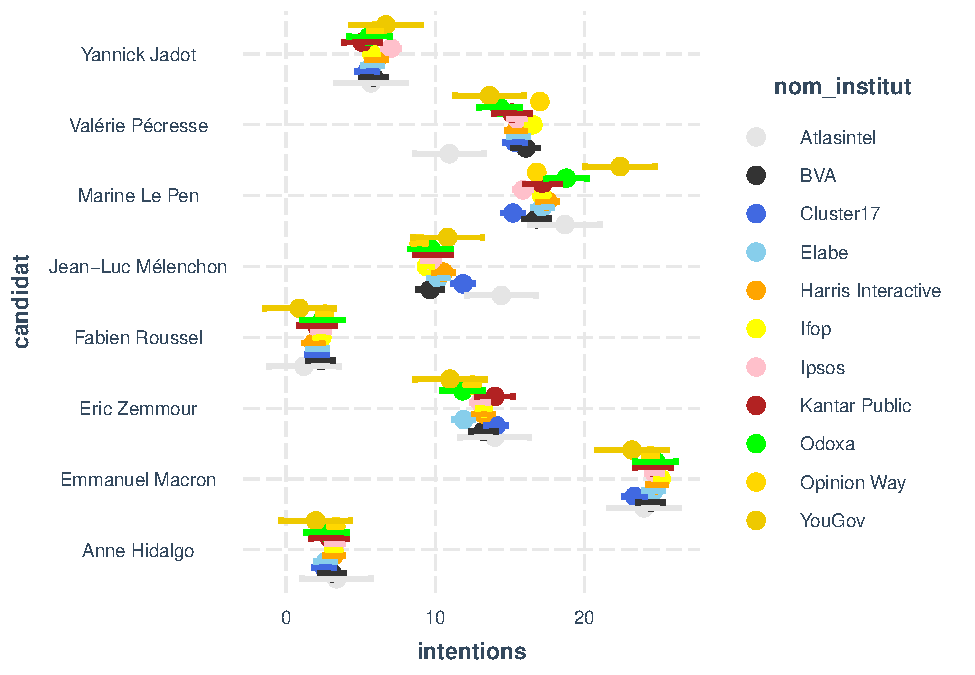
\includegraphics{bookdown-demo_files/figure-latex/biais-1.pdf}

\begin{Shaded}
\begin{Highlighting}[]
\FunctionTok{cat\_plot}\NormalTok{(fit2, }\AttributeTok{pred=}\NormalTok{ tps,}\AttributeTok{modx=}\NormalTok{candidat, }\AttributeTok{color.class=}\StringTok{"Spectral"}\NormalTok{, }\AttributeTok{dodge.width=}\DecValTok{0}\NormalTok{)}\SpecialCharTok{+}
  \FunctionTok{scale\_color\_manual}\NormalTok{(}\AttributeTok{values =}\NormalTok{ SensiP2)}\SpecialCharTok{+}\FunctionTok{geom\_line}\NormalTok{(}\FunctionTok{aes}\NormalTok{(}\AttributeTok{color=}\NormalTok{candidat))}
\end{Highlighting}
\end{Shaded}

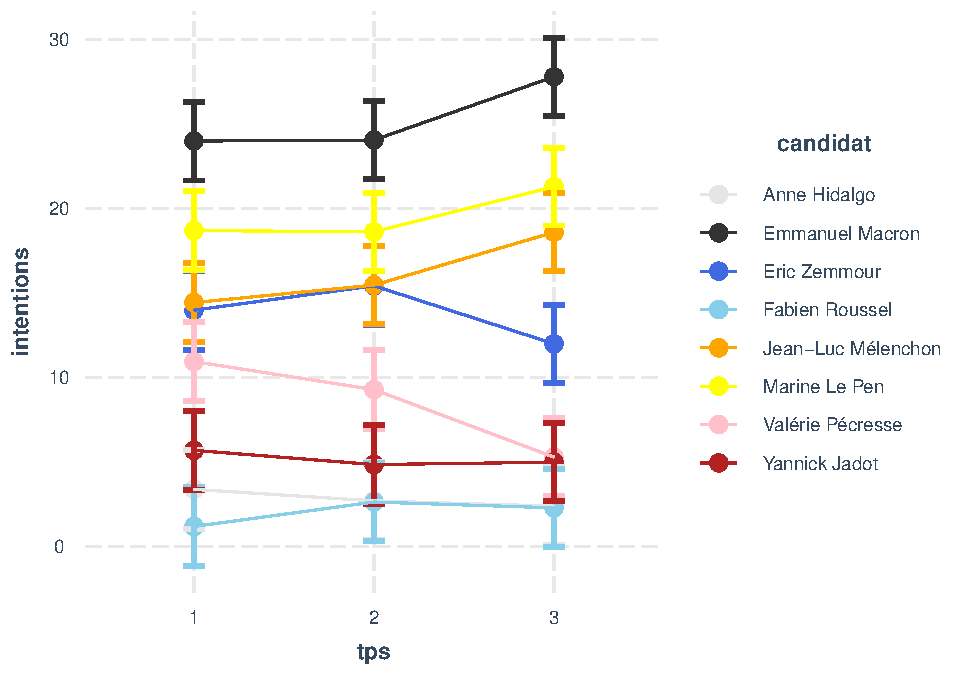
\includegraphics{bookdown-demo_files/figure-latex/biais-2.pdf}

\hypertarget{donnuxe9es-guxe9ographique}{%
\chapter{Données géographique}\label{donnuxe9es-guxe9ographique}}

voir étude de cas \href{http://r.benavent.fr/map.html}{Airbnb} avec le package sf

\hypertarget{analyses-factorielles-exploratoires}{%
\chapter{Analyses factorielles exploratoires}\label{analyses-factorielles-exploratoires}}

\hypertarget{origine-et-histoire}{%
\section{Origine et histoire}\label{origine-et-histoire}}

Par analyse factorielle, on entend finalement un ensemble de méthodes dont l'objectif est d'extraire d'un ensemble multivariée de données, un petit nombre de dimensions, les facteurs, qui rendent compte de l'essentiel des variations. On peut en distinguer deux écoles, l'une alimentée par des questions de psychométrie, plutôt américaine, et l'autre française s'intéresse aux variables qualitatives, et à une perspective plus descriptive.

\hypertarget{une-petite-histoire-de-la-psychomuxe9trie}{%
\subsection{Une petite histoire de la psychométrie}\label{une-petite-histoire-de-la-psychomuxe9trie}}

L'analyse factorielle trouve son origine, en psychologie, dans l'intuition que dans des épreuves multiples un facteur principal contrôle les variation des items (les performance à différents tests). Mais c'est avec \citet{thurstone_multiple_1931} que l'idée prend toute son ampleur en permettant que plusieurs facteurs traduisent la structure de la matrice de corrélations entre les tests. Spearman, Hotelling,.

Dans le monde de la gestion et en particulier de la GRH et du marketing, largement inspirés par la psychologie et la psychologie sociale, ces méthodes se sont propagées et ont formalisé un processus d'étude largement fondé sur ces techniques. Il est bien connu sous le terme de paradigme de Churchill qui synthésise une manière de construire et de développer des échelles multi-items de mesure par questionnaire.

Un grand virage c'est produit avec les méthodes d'équations structurelles qui ont permis le développement de méthodes à variables latente, dont la finalité est confirmatoire.

\hypertarget{luxe9cole-franuxe7aise-de-lanalyse-des-donnuxe9es-appliquuxe9e-aux-sciences-sociales}{%
\subsection{L'école française de l'analyse des données appliquée aux sciences sociales}\label{luxe9cole-franuxe7aise-de-lanalyse-des-donnuxe9es-appliquuxe9e-aux-sciences-sociales}}

dès le début des années 60

Un personnage : Emile Benzekri

Boudieu en premier applicateurs

Une école Française : pagès, escoffier, morisseau, Husson a repris le flambleau en développant FactoMiner.

Une série de logiciels : Alceste, Statitcf

\hypertarget{le-moduxe8le-en-facteurs-communs-et-spuxe9cifiques}{%
\section{Le modèle en facteurs communs et spécifiques}\label{le-moduxe8le-en-facteurs-communs-et-spuxe9cifiques}}

\hypertarget{un-peu-de-thuxe9orie}{%
\subsection{Un peu de théorie}\label{un-peu-de-thuxe9orie}}

La première historiquement est celle des psychologues et en particulier le modèle en terme de facteurs communs et spécifiques. Elle vise à partir de l'analyse d'une matrice de corrélation à identifier des éléments de structures sous-jascents.

La structure du modèle factoriel peut être présentée de manière simple. On supposera que chaque variables observées peut être décrites comme composées de facteurs généraux (\(F_{ik}\)) et de facteurs spécifiques \$ \varepsilon\_\{i\}\$. Le modèle suppose ainsi que la valeur de l'individu i pour la variable j, dépend de k facteurs sous-jacents, les facteurs communs, et d'un terme spécifique à l'item.

\[x_{ij}= a_{1j}F_{i1} + a_{2j}F_{i2} + \cdots + a_{jk}F_{ik}+\varepsilon_{ij}\]
On peut représenter cela de manière graphique, en utilisant les conventions symboliques des modèles structurels qu'on examine dans le chapitre SEM. On y verra d'ailleurs comment ce modèle peut être spécifié de manière confirmatoire. On remarquera que dans cette structure les facteurs peuvent être corrélés.

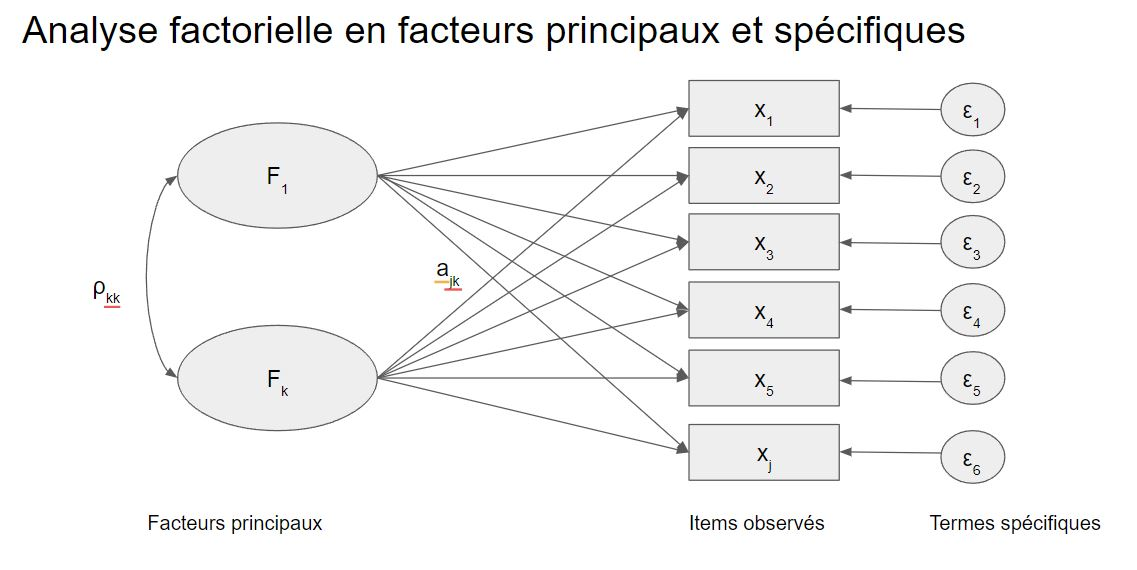
\includegraphics{./Images/FA01.jpg}
Certains lecteurs seront surpris de cette présentation, ils sont sans doute plus habitués à factoriser en employant une méthode de l' ACP. Effectivement cette méthode sur laquelle on va revenir avec plus de détail dans la seconde section de ce chapitre, est une des techniques qui permettent d'approcher le modèle théorique que l'on vient de présenter. Elle n'est pas la seule.

L'estimation du modèle requiert deux décisions : l'une sur la méthode d'extraction des facteurs, et l'autre sur la méthode de rotation.

Les méthodes d'extraction :
* ACP
* ML

Les méthodes de rotation.

\begin{itemize}
\tightlist
\item
  Varimax
\item
  Promax
\item
  Oblimin
\item
  \ldots{}
\end{itemize}

L'objectif des méthodes d'analyses factorielles est de réduire un ensemble de variables à un petit nombre de dimensions qui résument l'essentiel de l'information.

\hypertarget{ressources}{%
\subsection{Ressources}\label{ressources}}

On utilise principalement le package \texttt{psych} développé par Revelle et dédié à la psychométrie. Il couvre le plus complètement le champs de l'analyse factorielle et de la psychométrie.

S'y ajoutent deux fonctions très utiles pour représenter les résultats des analyses sous une forme lisible et au standard des publications scientifiques. Elles utilisent les ressources de \texttt{flextable}.

\begin{Shaded}
\begin{Highlighting}[]
\CommentTok{\# Une fonction utile pour créer }

\NormalTok{flex }\OtherTok{\textless{}{-}} \ControlFlowTok{function}\NormalTok{(data, }\AttributeTok{title=}\ConstantTok{NULL}\NormalTok{) \{}
  \CommentTok{\# this grabs the data and converts it to a flextbale}
  \FunctionTok{flextable}\NormalTok{(data) }\SpecialCharTok{\%\textgreater{}\%}
  \CommentTok{\# this makes the table fill the page width}
  \FunctionTok{set\_table\_properties}\NormalTok{(}\AttributeTok{layout =} \StringTok{"autofit"}\NormalTok{, }\AttributeTok{width =} \DecValTok{1}\NormalTok{) }\SpecialCharTok{\%\textgreater{}\%}
  \CommentTok{\# font size}
  \FunctionTok{fontsize}\NormalTok{(}\AttributeTok{size=}\DecValTok{10}\NormalTok{, }\AttributeTok{part=}\StringTok{"all"}\NormalTok{) }\SpecialCharTok{\%\textgreater{}\%}
    \CommentTok{\#this adds a ttitlecreates an automatic table number}
      \FunctionTok{set\_caption}\NormalTok{(title, }
                  \AttributeTok{autonum =}\NormalTok{ officer}\SpecialCharTok{::}\FunctionTok{run\_autonum}\NormalTok{(}\AttributeTok{seq\_id =} \StringTok{"tab"}\NormalTok{, }
                                                 \AttributeTok{pre\_label =} \StringTok{"Table "}\NormalTok{, }
                                                 \AttributeTok{post\_label =} \StringTok{"}\SpecialCharTok{\textbackslash{}n}\StringTok{"}\NormalTok{, }
                                                 \AttributeTok{bkm =} \StringTok{"anytable"}\NormalTok{)) }\SpecialCharTok{\%\textgreater{}\%}
  \CommentTok{\# font type}
  \FunctionTok{font}\NormalTok{(}\AttributeTok{fontname=}\StringTok{"Times New Roman"}\NormalTok{, }\AttributeTok{part=}\StringTok{"all"}\NormalTok{)}
\NormalTok{\}}

\CommentTok{\#Une seconde fonction pour le tableaux des loadings}

\NormalTok{fa\_table }\OtherTok{\textless{}{-}} \ControlFlowTok{function}\NormalTok{(x, cut) \{}
  \CommentTok{\#get sorted loadings}
\NormalTok{  loadings }\OtherTok{\textless{}{-}} \FunctionTok{fa.sort}\NormalTok{(x)}\SpecialCharTok{$}\NormalTok{loadings }\SpecialCharTok{\%\textgreater{}\%} \FunctionTok{round}\NormalTok{(}\DecValTok{3}\NormalTok{)}
  \CommentTok{\#supress loadings}
\NormalTok{  loadings[loadings }\SpecialCharTok{\textless{}}\NormalTok{ cut] }\OtherTok{\textless{}{-}} \StringTok{""}
  \CommentTok{\#get additional info}
\NormalTok{  add\_info }\OtherTok{\textless{}{-}} \FunctionTok{cbind}\NormalTok{(x}\SpecialCharTok{$}\NormalTok{communality, }
\NormalTok{                    x}\SpecialCharTok{$}\NormalTok{uniquenesses,}
\NormalTok{                    x}\SpecialCharTok{$}\NormalTok{complexity) }\SpecialCharTok{\%\textgreater{}\%}
    \CommentTok{\# make it a data frame}
    \FunctionTok{as.data.frame}\NormalTok{() }\SpecialCharTok{\%\textgreater{}\%}
    \CommentTok{\# column names}
    \FunctionTok{rename}\NormalTok{(}\StringTok{"Communality"} \OtherTok{=}\NormalTok{ V1,}
           \StringTok{"Uniqueness"} \OtherTok{=}\NormalTok{ V2,}
           \StringTok{"Complexity"} \OtherTok{=}\NormalTok{ V3) }\SpecialCharTok{\%\textgreater{}\%}
    \CommentTok{\#get the item names from the vector}
    \FunctionTok{rownames\_to\_column}\NormalTok{(}\StringTok{"item"}\NormalTok{)}
  \CommentTok{\#build table}
\NormalTok{  loadings }\SpecialCharTok{\%\textgreater{}\%}
    \FunctionTok{unclass}\NormalTok{() }\SpecialCharTok{\%\textgreater{}\%}
    \FunctionTok{as.data.frame}\NormalTok{() }\SpecialCharTok{\%\textgreater{}\%}
    \FunctionTok{rownames\_to\_column}\NormalTok{(}\StringTok{"item"}\NormalTok{) }\SpecialCharTok{\%\textgreater{}\%}
    \FunctionTok{left\_join}\NormalTok{(add\_info) }\SpecialCharTok{\%\textgreater{}\%}
    \FunctionTok{mutate}\NormalTok{(}\FunctionTok{across}\NormalTok{(}\FunctionTok{where}\NormalTok{(is.numeric), round, }\DecValTok{3}\NormalTok{))}
\NormalTok{\}}
\end{Highlighting}
\end{Shaded}

\hypertarget{cas-dapplication}{%
\section{Cas d'application}\label{cas-dapplication}}

Pour appliquer la méthode on va s'intéresser à l'échelle des valeurs de \citet{schwartz_les_2006}, qui sont mesurées dan différents pays au cours des différentes vagues de l'enquête European Social Survey.

Les variables mesurées sont un ensemble de 21 questions qui proposent des niveaux d'importances accordées à 21 questions, ou items, dont voici les formulation en anglais. Les répondants ont le choix sur une échelle de 0 à 10 qui va de ``pas du tout important'' à ``très important''. On se concentre sur les observations de la dernière vague.

Cette échelle a été développée par Schwartz

En voici les items dans leur formulation anglaise.

\begin{itemize}
\tightlist
\item
  IPCRTIV Important to think new ideas and being creative
\item
  IMPRICH Important to be rich, have money and expensive things
\item
  IPEQOPT Important that people are treated equally and have equal opportunities
\item
  IPSHABT Important to show abilities and be admired
\item
  IMPSAFE Important to live in secure and safe surroundings
\item
  IMPDIFF Important to try new and different things in life
\item
  IPFRULE Important to do what is told and follow rules
\item
  IPUDRST Important to understand different people
\item
  IPMODST Important to be humble and modest, not draw attention
\item
  IPGDTIM Important to have a good time
\item
  IMPFREE Important to make own decisions and be free
\item
  IPHLPPL Important to help people and care for others well-being
\item
  IPSUCES Important to be successful and that people recognise achievements
\item
  IPSTRGV Important that government is strong and ensures safety
\item
  IPADVNT Important to seek adventures and have an exciting life
\item
  IPBHPRP Important to behave properly
\item
  IPRSPOT Important to get respect from others
\item
  IPLYLFR Important to be loyal to friends and devote to people close
\item
  IMPENV Important to care for nature and environment
\item
  IMPTRAD Important to follow traditions and customs
\item
  IMPFUN Important to seek fun and things that give pleasure
\end{itemize}

\begin{Shaded}
\begin{Highlighting}[]
\CommentTok{\# On renomme les variables pour une meilleure lecture et on selectionne }
\CommentTok{\# le tableau de données utile à l\textquotesingle{}analyse.}

\NormalTok{df }\OtherTok{\textless{}{-}} \FunctionTok{read\_csv}\NormalTok{(}\StringTok{"./Data/ESS1{-}9e01\_1.csv"}\NormalTok{) }\SpecialCharTok{\%\textgreater{}\%}
  \FunctionTok{rename}\NormalTok{(}
    \AttributeTok{V\_creative=}\NormalTok{ipcrtiv,}
    \AttributeTok{V\_richness=}\NormalTok{ imprich,}
    \AttributeTok{V\_justice =}\NormalTok{ipeqopt, }
    \AttributeTok{V\_admiration=}\NormalTok{ipshabt, }
    \AttributeTok{V\_security=}\NormalTok{impsafe, }
    \AttributeTok{V\_novelty=}\NormalTok{impdiff, }
    \AttributeTok{V\_conformism=}\NormalTok{ipfrule, }
    \AttributeTok{V\_openmindedness=}\NormalTok{ipudrst, }
    \AttributeTok{V\_modesty=}\NormalTok{ipmodst, }
    \AttributeTok{V\_fun=}\NormalTok{ipgdtim, }
    \AttributeTok{V\_autonomy=}\NormalTok{impfree, }
    \AttributeTok{V\_Care=}\NormalTok{iphlppl, }
    \AttributeTok{V\_Success=}\NormalTok{ipsuces,}
    \AttributeTok{V\_Autority =}\NormalTok{ipstrgv, }
    \AttributeTok{V\_Adventures=}\NormalTok{ipadvnt,}
    \AttributeTok{V\_wellbehavior=}\NormalTok{ipbhprp,}
    \AttributeTok{V\_respect=}\NormalTok{iprspot,}
    \AttributeTok{V\_loyalty=}\NormalTok{iplylfr,}
    \AttributeTok{V\_environnement=}\NormalTok{impenv,}
    \AttributeTok{V\_tradition=}\NormalTok{imptrad, }
    \AttributeTok{V\_pleasure=}\NormalTok{impfun)}

\NormalTok{foo1}\OtherTok{\textless{}{-}}\NormalTok{df }\SpecialCharTok{\%\textgreater{}\%} \FunctionTok{filter}\NormalTok{(essround}\SpecialCharTok{==}\DecValTok{9}\NormalTok{)}\SpecialCharTok{\%\textgreater{}\%}
\NormalTok{  dplyr}\SpecialCharTok{::}\FunctionTok{select}\NormalTok{(}\FunctionTok{matches}\NormalTok{(}\StringTok{"V\_.*"}\NormalTok{), cntry) }\SpecialCharTok{\%\textgreater{}\%} \CommentTok{\#notons la selection fondée sur des regex}
  \FunctionTok{drop\_na}\NormalTok{()}
\end{Highlighting}
\end{Shaded}

\hypertarget{examen-de-la-matrice-de-corruxe9lation}{%
\subsection{Examen de la matrice de corrélation}\label{examen-de-la-matrice-de-corruxe9lation}}

Calculons la matrice de corrélation, et présentons là en organisant l'ordre des variables selon leur corrélation. A ce stade indiquons qu'il s'agit de mettre un ordre dans les variables, tel que des variables fortement corrélées soient adjascentes (on revient sur la méthode utilisée dans le chapitre suivant).

On s'aperçoit qu'une structure émerge. Quatre groupes de variables peuvent être discernés:
* la jouissance
* le succès social
* l'ouverture aux autres
* la sécurité

Dans le filigrane de la matrice de corrélation, on devine une structure factorielle.

\begin{Shaded}
\begin{Highlighting}[]
\NormalTok{foo}\OtherTok{\textless{}{-}}\NormalTok{ foo1 }\SpecialCharTok{\%\textgreater{}\%} 
\NormalTok{  dplyr}\SpecialCharTok{::}\FunctionTok{select}\NormalTok{(}\FunctionTok{matches}\NormalTok{(}\StringTok{"V\_.*"}\NormalTok{))}

\NormalTok{M }\OtherTok{\textless{}{-}} \FunctionTok{cor}\NormalTok{(foo)}

\FunctionTok{ggcorrplot}\NormalTok{(M, }\AttributeTok{hc.order =} \ConstantTok{TRUE}\NormalTok{, }\AttributeTok{type =} \StringTok{"lower"}\NormalTok{,}
   \AttributeTok{outline.col =} \StringTok{"white"}\NormalTok{,}
   \AttributeTok{ggtheme =}\NormalTok{ ggplot2}\SpecialCharTok{::}\NormalTok{theme\_gray,}
   \AttributeTok{colors =} \FunctionTok{c}\NormalTok{(}\StringTok{"\#6D9EC1"}\NormalTok{, }\StringTok{"white"}\NormalTok{, }\StringTok{"\#E46726"}\NormalTok{), }\AttributeTok{lab =} \ConstantTok{TRUE}\NormalTok{, }\AttributeTok{lab\_size =} \DecValTok{4}\NormalTok{)}
\end{Highlighting}
\end{Shaded}

\includegraphics{bookdown-demo_files/figure-latex/0603b-1.pdf}

\hypertarget{moduxe8le-factoriel}{%
\subsection{Modèle factoriel}\label{moduxe8le-factoriel}}

Testons un modèle d'analyse factorielle à 4 dimensions. Nous l'augmentons d'un procédure de rotation oblimin pour un meilleur ajustement.

\begin{Shaded}
\begin{Highlighting}[]
\NormalTok{fa }\OtherTok{\textless{}{-}} \FunctionTok{fa}\NormalTok{(foo,}\DecValTok{4}\NormalTok{, }\AttributeTok{rotate=}\StringTok{"oblimin"}\NormalTok{)  }\CommentTok{\#principal axis }

\FunctionTok{fa\_table}\NormalTok{(fa, .}\DecValTok{30}\NormalTok{)}\SpecialCharTok{\%\textgreater{}\%}
  \FunctionTok{flex}\NormalTok{(}\StringTok{"A Pretty Factor Analysis Table"}\NormalTok{)}
\end{Highlighting}
\end{Shaded}

\providecommand{\docline}[3]{\noalign{\global\setlength{\arrayrulewidth}{#1}}\arrayrulecolor[HTML]{#2}\cline{#3}}

\setlength{\tabcolsep}{2pt}

\renewcommand*{\arraystretch}{1.5}

\begin{longtable}[c]{cccccccc}

\caption{A Pretty Factor Analysis Table}\label{tab:anytable}\\

\hhline{>{\arrayrulecolor[HTML]{666666}\global\arrayrulewidth=2pt}->{\arrayrulecolor[HTML]{666666}\global\arrayrulewidth=2pt}->{\arrayrulecolor[HTML]{666666}\global\arrayrulewidth=2pt}->{\arrayrulecolor[HTML]{666666}\global\arrayrulewidth=2pt}->{\arrayrulecolor[HTML]{666666}\global\arrayrulewidth=2pt}->{\arrayrulecolor[HTML]{666666}\global\arrayrulewidth=2pt}->{\arrayrulecolor[HTML]{666666}\global\arrayrulewidth=2pt}->{\arrayrulecolor[HTML]{666666}\global\arrayrulewidth=2pt}-}

\multicolumn{1}{!{\color[HTML]{000000}\vrule width 0pt}>{}l}{\fontsize{10}{10}\selectfont{\textcolor[HTML]{000000}{\global\setmainfont{Times New Roman}{item}}}} & \multicolumn{1}{!{\color[HTML]{000000}\vrule width 0pt}>{}l}{\fontsize{10}{10}\selectfont{\textcolor[HTML]{000000}{\global\setmainfont{Times New Roman}{MR1}}}} & \multicolumn{1}{!{\color[HTML]{000000}\vrule width 0pt}>{}l}{\fontsize{10}{10}\selectfont{\textcolor[HTML]{000000}{\global\setmainfont{Times New Roman}{MR4}}}} & \multicolumn{1}{!{\color[HTML]{000000}\vrule width 0pt}>{}l}{\fontsize{10}{10}\selectfont{\textcolor[HTML]{000000}{\global\setmainfont{Times New Roman}{MR3}}}} & \multicolumn{1}{!{\color[HTML]{000000}\vrule width 0pt}>{}l}{\fontsize{10}{10}\selectfont{\textcolor[HTML]{000000}{\global\setmainfont{Times New Roman}{MR2}}}} & \multicolumn{1}{!{\color[HTML]{000000}\vrule width 0pt}>{}r}{\fontsize{10}{10}\selectfont{\textcolor[HTML]{000000}{\global\setmainfont{Times New Roman}{Communality}}}} & \multicolumn{1}{!{\color[HTML]{000000}\vrule width 0pt}>{}r}{\fontsize{10}{10}\selectfont{\textcolor[HTML]{000000}{\global\setmainfont{Times New Roman}{Uniqueness}}}} & \multicolumn{1}{!{\color[HTML]{000000}\vrule width 0pt}>{}r!{\color[HTML]{000000}\vrule width 0pt}}{\fontsize{10}{10}\selectfont{\textcolor[HTML]{000000}{\global\setmainfont{Times New Roman}{Complexity}}}} \\

\noalign{\global\setlength{\arrayrulewidth}{2pt}}\arrayrulecolor[HTML]{666666}\cline{1-8}

\endfirsthead

\hhline{>{\arrayrulecolor[HTML]{666666}\global\arrayrulewidth=2pt}->{\arrayrulecolor[HTML]{666666}\global\arrayrulewidth=2pt}->{\arrayrulecolor[HTML]{666666}\global\arrayrulewidth=2pt}->{\arrayrulecolor[HTML]{666666}\global\arrayrulewidth=2pt}->{\arrayrulecolor[HTML]{666666}\global\arrayrulewidth=2pt}->{\arrayrulecolor[HTML]{666666}\global\arrayrulewidth=2pt}->{\arrayrulecolor[HTML]{666666}\global\arrayrulewidth=2pt}->{\arrayrulecolor[HTML]{666666}\global\arrayrulewidth=2pt}-}

\multicolumn{1}{!{\color[HTML]{000000}\vrule width 0pt}>{}l}{\fontsize{10}{10}\selectfont{\textcolor[HTML]{000000}{\global\setmainfont{Times New Roman}{item}}}} & \multicolumn{1}{!{\color[HTML]{000000}\vrule width 0pt}>{}l}{\fontsize{10}{10}\selectfont{\textcolor[HTML]{000000}{\global\setmainfont{Times New Roman}{MR1}}}} & \multicolumn{1}{!{\color[HTML]{000000}\vrule width 0pt}>{}l}{\fontsize{10}{10}\selectfont{\textcolor[HTML]{000000}{\global\setmainfont{Times New Roman}{MR4}}}} & \multicolumn{1}{!{\color[HTML]{000000}\vrule width 0pt}>{}l}{\fontsize{10}{10}\selectfont{\textcolor[HTML]{000000}{\global\setmainfont{Times New Roman}{MR3}}}} & \multicolumn{1}{!{\color[HTML]{000000}\vrule width 0pt}>{}l}{\fontsize{10}{10}\selectfont{\textcolor[HTML]{000000}{\global\setmainfont{Times New Roman}{MR2}}}} & \multicolumn{1}{!{\color[HTML]{000000}\vrule width 0pt}>{}r}{\fontsize{10}{10}\selectfont{\textcolor[HTML]{000000}{\global\setmainfont{Times New Roman}{Communality}}}} & \multicolumn{1}{!{\color[HTML]{000000}\vrule width 0pt}>{}r}{\fontsize{10}{10}\selectfont{\textcolor[HTML]{000000}{\global\setmainfont{Times New Roman}{Uniqueness}}}} & \multicolumn{1}{!{\color[HTML]{000000}\vrule width 0pt}>{}r!{\color[HTML]{000000}\vrule width 0pt}}{\fontsize{10}{10}\selectfont{\textcolor[HTML]{000000}{\global\setmainfont{Times New Roman}{Complexity}}}} \\

\noalign{\global\setlength{\arrayrulewidth}{2pt}}\arrayrulecolor[HTML]{666666}\cline{1-8}\endhead



\multicolumn{1}{!{\color[HTML]{000000}\vrule width 0pt}>{}l}{\fontsize{10}{10}\selectfont{\textcolor[HTML]{000000}{\global\setmainfont{Times New Roman}{V\_openmindedness}}}} & \multicolumn{1}{!{\color[HTML]{000000}\vrule width 0pt}>{}l}{\fontsize{10}{10}\selectfont{\textcolor[HTML]{000000}{\global\setmainfont{Times New Roman}{0.692}}}} & \multicolumn{1}{!{\color[HTML]{000000}\vrule width 0pt}>{}l}{\fontsize{10}{10}\selectfont{\textcolor[HTML]{000000}{\global\setmainfont{Times New Roman}{}}}} & \multicolumn{1}{!{\color[HTML]{000000}\vrule width 0pt}>{}l}{\fontsize{10}{10}\selectfont{\textcolor[HTML]{000000}{\global\setmainfont{Times New Roman}{}}}} & \multicolumn{1}{!{\color[HTML]{000000}\vrule width 0pt}>{}l}{\fontsize{10}{10}\selectfont{\textcolor[HTML]{000000}{\global\setmainfont{Times New Roman}{}}}} & \multicolumn{1}{!{\color[HTML]{000000}\vrule width 0pt}>{}r}{\fontsize{10}{10}\selectfont{\textcolor[HTML]{000000}{\global\setmainfont{Times New Roman}{0.472}}}} & \multicolumn{1}{!{\color[HTML]{000000}\vrule width 0pt}>{}r}{\fontsize{10}{10}\selectfont{\textcolor[HTML]{000000}{\global\setmainfont{Times New Roman}{0.528}}}} & \multicolumn{1}{!{\color[HTML]{000000}\vrule width 0pt}>{}r!{\color[HTML]{000000}\vrule width 0pt}}{\fontsize{10}{10}\selectfont{\textcolor[HTML]{000000}{\global\setmainfont{Times New Roman}{1.002}}}} \\





\multicolumn{1}{!{\color[HTML]{000000}\vrule width 0pt}>{}l}{\fontsize{10}{10}\selectfont{\textcolor[HTML]{000000}{\global\setmainfont{Times New Roman}{V\_justice}}}} & \multicolumn{1}{!{\color[HTML]{000000}\vrule width 0pt}>{}l}{\fontsize{10}{10}\selectfont{\textcolor[HTML]{000000}{\global\setmainfont{Times New Roman}{0.665}}}} & \multicolumn{1}{!{\color[HTML]{000000}\vrule width 0pt}>{}l}{\fontsize{10}{10}\selectfont{\textcolor[HTML]{000000}{\global\setmainfont{Times New Roman}{}}}} & \multicolumn{1}{!{\color[HTML]{000000}\vrule width 0pt}>{}l}{\fontsize{10}{10}\selectfont{\textcolor[HTML]{000000}{\global\setmainfont{Times New Roman}{}}}} & \multicolumn{1}{!{\color[HTML]{000000}\vrule width 0pt}>{}l}{\fontsize{10}{10}\selectfont{\textcolor[HTML]{000000}{\global\setmainfont{Times New Roman}{}}}} & \multicolumn{1}{!{\color[HTML]{000000}\vrule width 0pt}>{}r}{\fontsize{10}{10}\selectfont{\textcolor[HTML]{000000}{\global\setmainfont{Times New Roman}{0.399}}}} & \multicolumn{1}{!{\color[HTML]{000000}\vrule width 0pt}>{}r}{\fontsize{10}{10}\selectfont{\textcolor[HTML]{000000}{\global\setmainfont{Times New Roman}{0.601}}}} & \multicolumn{1}{!{\color[HTML]{000000}\vrule width 0pt}>{}r!{\color[HTML]{000000}\vrule width 0pt}}{\fontsize{10}{10}\selectfont{\textcolor[HTML]{000000}{\global\setmainfont{Times New Roman}{1.044}}}} \\





\multicolumn{1}{!{\color[HTML]{000000}\vrule width 0pt}>{}l}{\fontsize{10}{10}\selectfont{\textcolor[HTML]{000000}{\global\setmainfont{Times New Roman}{V\_Care}}}} & \multicolumn{1}{!{\color[HTML]{000000}\vrule width 0pt}>{}l}{\fontsize{10}{10}\selectfont{\textcolor[HTML]{000000}{\global\setmainfont{Times New Roman}{0.621}}}} & \multicolumn{1}{!{\color[HTML]{000000}\vrule width 0pt}>{}l}{\fontsize{10}{10}\selectfont{\textcolor[HTML]{000000}{\global\setmainfont{Times New Roman}{}}}} & \multicolumn{1}{!{\color[HTML]{000000}\vrule width 0pt}>{}l}{\fontsize{10}{10}\selectfont{\textcolor[HTML]{000000}{\global\setmainfont{Times New Roman}{}}}} & \multicolumn{1}{!{\color[HTML]{000000}\vrule width 0pt}>{}l}{\fontsize{10}{10}\selectfont{\textcolor[HTML]{000000}{\global\setmainfont{Times New Roman}{}}}} & \multicolumn{1}{!{\color[HTML]{000000}\vrule width 0pt}>{}r}{\fontsize{10}{10}\selectfont{\textcolor[HTML]{000000}{\global\setmainfont{Times New Roman}{0.516}}}} & \multicolumn{1}{!{\color[HTML]{000000}\vrule width 0pt}>{}r}{\fontsize{10}{10}\selectfont{\textcolor[HTML]{000000}{\global\setmainfont{Times New Roman}{0.484}}}} & \multicolumn{1}{!{\color[HTML]{000000}\vrule width 0pt}>{}r!{\color[HTML]{000000}\vrule width 0pt}}{\fontsize{10}{10}\selectfont{\textcolor[HTML]{000000}{\global\setmainfont{Times New Roman}{1.145}}}} \\





\multicolumn{1}{!{\color[HTML]{000000}\vrule width 0pt}>{}l}{\fontsize{10}{10}\selectfont{\textcolor[HTML]{000000}{\global\setmainfont{Times New Roman}{V\_environnement}}}} & \multicolumn{1}{!{\color[HTML]{000000}\vrule width 0pt}>{}l}{\fontsize{10}{10}\selectfont{\textcolor[HTML]{000000}{\global\setmainfont{Times New Roman}{0.561}}}} & \multicolumn{1}{!{\color[HTML]{000000}\vrule width 0pt}>{}l}{\fontsize{10}{10}\selectfont{\textcolor[HTML]{000000}{\global\setmainfont{Times New Roman}{}}}} & \multicolumn{1}{!{\color[HTML]{000000}\vrule width 0pt}>{}l}{\fontsize{10}{10}\selectfont{\textcolor[HTML]{000000}{\global\setmainfont{Times New Roman}{}}}} & \multicolumn{1}{!{\color[HTML]{000000}\vrule width 0pt}>{}l}{\fontsize{10}{10}\selectfont{\textcolor[HTML]{000000}{\global\setmainfont{Times New Roman}{}}}} & \multicolumn{1}{!{\color[HTML]{000000}\vrule width 0pt}>{}r}{\fontsize{10}{10}\selectfont{\textcolor[HTML]{000000}{\global\setmainfont{Times New Roman}{0.427}}}} & \multicolumn{1}{!{\color[HTML]{000000}\vrule width 0pt}>{}r}{\fontsize{10}{10}\selectfont{\textcolor[HTML]{000000}{\global\setmainfont{Times New Roman}{0.573}}}} & \multicolumn{1}{!{\color[HTML]{000000}\vrule width 0pt}>{}r!{\color[HTML]{000000}\vrule width 0pt}}{\fontsize{10}{10}\selectfont{\textcolor[HTML]{000000}{\global\setmainfont{Times New Roman}{1.171}}}} \\





\multicolumn{1}{!{\color[HTML]{000000}\vrule width 0pt}>{}l}{\fontsize{10}{10}\selectfont{\textcolor[HTML]{000000}{\global\setmainfont{Times New Roman}{V\_loyalty}}}} & \multicolumn{1}{!{\color[HTML]{000000}\vrule width 0pt}>{}l}{\fontsize{10}{10}\selectfont{\textcolor[HTML]{000000}{\global\setmainfont{Times New Roman}{0.518}}}} & \multicolumn{1}{!{\color[HTML]{000000}\vrule width 0pt}>{}l}{\fontsize{10}{10}\selectfont{\textcolor[HTML]{000000}{\global\setmainfont{Times New Roman}{}}}} & \multicolumn{1}{!{\color[HTML]{000000}\vrule width 0pt}>{}l}{\fontsize{10}{10}\selectfont{\textcolor[HTML]{000000}{\global\setmainfont{Times New Roman}{}}}} & \multicolumn{1}{!{\color[HTML]{000000}\vrule width 0pt}>{}l}{\fontsize{10}{10}\selectfont{\textcolor[HTML]{000000}{\global\setmainfont{Times New Roman}{}}}} & \multicolumn{1}{!{\color[HTML]{000000}\vrule width 0pt}>{}r}{\fontsize{10}{10}\selectfont{\textcolor[HTML]{000000}{\global\setmainfont{Times New Roman}{0.493}}}} & \multicolumn{1}{!{\color[HTML]{000000}\vrule width 0pt}>{}r}{\fontsize{10}{10}\selectfont{\textcolor[HTML]{000000}{\global\setmainfont{Times New Roman}{0.507}}}} & \multicolumn{1}{!{\color[HTML]{000000}\vrule width 0pt}>{}r!{\color[HTML]{000000}\vrule width 0pt}}{\fontsize{10}{10}\selectfont{\textcolor[HTML]{000000}{\global\setmainfont{Times New Roman}{1.570}}}} \\





\multicolumn{1}{!{\color[HTML]{000000}\vrule width 0pt}>{}l}{\fontsize{10}{10}\selectfont{\textcolor[HTML]{000000}{\global\setmainfont{Times New Roman}{V\_autonomy}}}} & \multicolumn{1}{!{\color[HTML]{000000}\vrule width 0pt}>{}l}{\fontsize{10}{10}\selectfont{\textcolor[HTML]{000000}{\global\setmainfont{Times New Roman}{0.438}}}} & \multicolumn{1}{!{\color[HTML]{000000}\vrule width 0pt}>{}l}{\fontsize{10}{10}\selectfont{\textcolor[HTML]{000000}{\global\setmainfont{Times New Roman}{}}}} & \multicolumn{1}{!{\color[HTML]{000000}\vrule width 0pt}>{}l}{\fontsize{10}{10}\selectfont{\textcolor[HTML]{000000}{\global\setmainfont{Times New Roman}{}}}} & \multicolumn{1}{!{\color[HTML]{000000}\vrule width 0pt}>{}l}{\fontsize{10}{10}\selectfont{\textcolor[HTML]{000000}{\global\setmainfont{Times New Roman}{}}}} & \multicolumn{1}{!{\color[HTML]{000000}\vrule width 0pt}>{}r}{\fontsize{10}{10}\selectfont{\textcolor[HTML]{000000}{\global\setmainfont{Times New Roman}{0.364}}}} & \multicolumn{1}{!{\color[HTML]{000000}\vrule width 0pt}>{}r}{\fontsize{10}{10}\selectfont{\textcolor[HTML]{000000}{\global\setmainfont{Times New Roman}{0.636}}}} & \multicolumn{1}{!{\color[HTML]{000000}\vrule width 0pt}>{}r!{\color[HTML]{000000}\vrule width 0pt}}{\fontsize{10}{10}\selectfont{\textcolor[HTML]{000000}{\global\setmainfont{Times New Roman}{1.603}}}} \\





\multicolumn{1}{!{\color[HTML]{000000}\vrule width 0pt}>{}l}{\fontsize{10}{10}\selectfont{\textcolor[HTML]{000000}{\global\setmainfont{Times New Roman}{V\_creative}}}} & \multicolumn{1}{!{\color[HTML]{000000}\vrule width 0pt}>{}l}{\fontsize{10}{10}\selectfont{\textcolor[HTML]{000000}{\global\setmainfont{Times New Roman}{0.429}}}} & \multicolumn{1}{!{\color[HTML]{000000}\vrule width 0pt}>{}l}{\fontsize{10}{10}\selectfont{\textcolor[HTML]{000000}{\global\setmainfont{Times New Roman}{}}}} & \multicolumn{1}{!{\color[HTML]{000000}\vrule width 0pt}>{}l}{\fontsize{10}{10}\selectfont{\textcolor[HTML]{000000}{\global\setmainfont{Times New Roman}{}}}} & \multicolumn{1}{!{\color[HTML]{000000}\vrule width 0pt}>{}l}{\fontsize{10}{10}\selectfont{\textcolor[HTML]{000000}{\global\setmainfont{Times New Roman}{}}}} & \multicolumn{1}{!{\color[HTML]{000000}\vrule width 0pt}>{}r}{\fontsize{10}{10}\selectfont{\textcolor[HTML]{000000}{\global\setmainfont{Times New Roman}{0.341}}}} & \multicolumn{1}{!{\color[HTML]{000000}\vrule width 0pt}>{}r}{\fontsize{10}{10}\selectfont{\textcolor[HTML]{000000}{\global\setmainfont{Times New Roman}{0.659}}}} & \multicolumn{1}{!{\color[HTML]{000000}\vrule width 0pt}>{}r!{\color[HTML]{000000}\vrule width 0pt}}{\fontsize{10}{10}\selectfont{\textcolor[HTML]{000000}{\global\setmainfont{Times New Roman}{2.225}}}} \\





\multicolumn{1}{!{\color[HTML]{000000}\vrule width 0pt}>{}l}{\fontsize{10}{10}\selectfont{\textcolor[HTML]{000000}{\global\setmainfont{Times New Roman}{V\_modesty}}}} & \multicolumn{1}{!{\color[HTML]{000000}\vrule width 0pt}>{}l}{\fontsize{10}{10}\selectfont{\textcolor[HTML]{000000}{\global\setmainfont{Times New Roman}{0.421}}}} & \multicolumn{1}{!{\color[HTML]{000000}\vrule width 0pt}>{}l}{\fontsize{10}{10}\selectfont{\textcolor[HTML]{000000}{\global\setmainfont{Times New Roman}{}}}} & \multicolumn{1}{!{\color[HTML]{000000}\vrule width 0pt}>{}l}{\fontsize{10}{10}\selectfont{\textcolor[HTML]{000000}{\global\setmainfont{Times New Roman}{0.301}}}} & \multicolumn{1}{!{\color[HTML]{000000}\vrule width 0pt}>{}l}{\fontsize{10}{10}\selectfont{\textcolor[HTML]{000000}{\global\setmainfont{Times New Roman}{}}}} & \multicolumn{1}{!{\color[HTML]{000000}\vrule width 0pt}>{}r}{\fontsize{10}{10}\selectfont{\textcolor[HTML]{000000}{\global\setmainfont{Times New Roman}{0.339}}}} & \multicolumn{1}{!{\color[HTML]{000000}\vrule width 0pt}>{}r}{\fontsize{10}{10}\selectfont{\textcolor[HTML]{000000}{\global\setmainfont{Times New Roman}{0.661}}}} & \multicolumn{1}{!{\color[HTML]{000000}\vrule width 0pt}>{}r!{\color[HTML]{000000}\vrule width 0pt}}{\fontsize{10}{10}\selectfont{\textcolor[HTML]{000000}{\global\setmainfont{Times New Roman}{1.967}}}} \\





\multicolumn{1}{!{\color[HTML]{000000}\vrule width 0pt}>{}l}{\fontsize{10}{10}\selectfont{\textcolor[HTML]{000000}{\global\setmainfont{Times New Roman}{V\_admiration}}}} & \multicolumn{1}{!{\color[HTML]{000000}\vrule width 0pt}>{}l}{\fontsize{10}{10}\selectfont{\textcolor[HTML]{000000}{\global\setmainfont{Times New Roman}{}}}} & \multicolumn{1}{!{\color[HTML]{000000}\vrule width 0pt}>{}l}{\fontsize{10}{10}\selectfont{\textcolor[HTML]{000000}{\global\setmainfont{Times New Roman}{0.697}}}} & \multicolumn{1}{!{\color[HTML]{000000}\vrule width 0pt}>{}l}{\fontsize{10}{10}\selectfont{\textcolor[HTML]{000000}{\global\setmainfont{Times New Roman}{}}}} & \multicolumn{1}{!{\color[HTML]{000000}\vrule width 0pt}>{}l}{\fontsize{10}{10}\selectfont{\textcolor[HTML]{000000}{\global\setmainfont{Times New Roman}{}}}} & \multicolumn{1}{!{\color[HTML]{000000}\vrule width 0pt}>{}r}{\fontsize{10}{10}\selectfont{\textcolor[HTML]{000000}{\global\setmainfont{Times New Roman}{0.505}}}} & \multicolumn{1}{!{\color[HTML]{000000}\vrule width 0pt}>{}r}{\fontsize{10}{10}\selectfont{\textcolor[HTML]{000000}{\global\setmainfont{Times New Roman}{0.495}}}} & \multicolumn{1}{!{\color[HTML]{000000}\vrule width 0pt}>{}r!{\color[HTML]{000000}\vrule width 0pt}}{\fontsize{10}{10}\selectfont{\textcolor[HTML]{000000}{\global\setmainfont{Times New Roman}{1.049}}}} \\





\multicolumn{1}{!{\color[HTML]{000000}\vrule width 0pt}>{}l}{\fontsize{10}{10}\selectfont{\textcolor[HTML]{000000}{\global\setmainfont{Times New Roman}{V\_Success}}}} & \multicolumn{1}{!{\color[HTML]{000000}\vrule width 0pt}>{}l}{\fontsize{10}{10}\selectfont{\textcolor[HTML]{000000}{\global\setmainfont{Times New Roman}{}}}} & \multicolumn{1}{!{\color[HTML]{000000}\vrule width 0pt}>{}l}{\fontsize{10}{10}\selectfont{\textcolor[HTML]{000000}{\global\setmainfont{Times New Roman}{0.644}}}} & \multicolumn{1}{!{\color[HTML]{000000}\vrule width 0pt}>{}l}{\fontsize{10}{10}\selectfont{\textcolor[HTML]{000000}{\global\setmainfont{Times New Roman}{}}}} & \multicolumn{1}{!{\color[HTML]{000000}\vrule width 0pt}>{}l}{\fontsize{10}{10}\selectfont{\textcolor[HTML]{000000}{\global\setmainfont{Times New Roman}{}}}} & \multicolumn{1}{!{\color[HTML]{000000}\vrule width 0pt}>{}r}{\fontsize{10}{10}\selectfont{\textcolor[HTML]{000000}{\global\setmainfont{Times New Roman}{0.539}}}} & \multicolumn{1}{!{\color[HTML]{000000}\vrule width 0pt}>{}r}{\fontsize{10}{10}\selectfont{\textcolor[HTML]{000000}{\global\setmainfont{Times New Roman}{0.461}}}} & \multicolumn{1}{!{\color[HTML]{000000}\vrule width 0pt}>{}r!{\color[HTML]{000000}\vrule width 0pt}}{\fontsize{10}{10}\selectfont{\textcolor[HTML]{000000}{\global\setmainfont{Times New Roman}{1.094}}}} \\





\multicolumn{1}{!{\color[HTML]{000000}\vrule width 0pt}>{}l}{\fontsize{10}{10}\selectfont{\textcolor[HTML]{000000}{\global\setmainfont{Times New Roman}{V\_richness}}}} & \multicolumn{1}{!{\color[HTML]{000000}\vrule width 0pt}>{}l}{\fontsize{10}{10}\selectfont{\textcolor[HTML]{000000}{\global\setmainfont{Times New Roman}{}}}} & \multicolumn{1}{!{\color[HTML]{000000}\vrule width 0pt}>{}l}{\fontsize{10}{10}\selectfont{\textcolor[HTML]{000000}{\global\setmainfont{Times New Roman}{0.526}}}} & \multicolumn{1}{!{\color[HTML]{000000}\vrule width 0pt}>{}l}{\fontsize{10}{10}\selectfont{\textcolor[HTML]{000000}{\global\setmainfont{Times New Roman}{}}}} & \multicolumn{1}{!{\color[HTML]{000000}\vrule width 0pt}>{}l}{\fontsize{10}{10}\selectfont{\textcolor[HTML]{000000}{\global\setmainfont{Times New Roman}{}}}} & \multicolumn{1}{!{\color[HTML]{000000}\vrule width 0pt}>{}r}{\fontsize{10}{10}\selectfont{\textcolor[HTML]{000000}{\global\setmainfont{Times New Roman}{0.336}}}} & \multicolumn{1}{!{\color[HTML]{000000}\vrule width 0pt}>{}r}{\fontsize{10}{10}\selectfont{\textcolor[HTML]{000000}{\global\setmainfont{Times New Roman}{0.664}}}} & \multicolumn{1}{!{\color[HTML]{000000}\vrule width 0pt}>{}r!{\color[HTML]{000000}\vrule width 0pt}}{\fontsize{10}{10}\selectfont{\textcolor[HTML]{000000}{\global\setmainfont{Times New Roman}{1.402}}}} \\





\multicolumn{1}{!{\color[HTML]{000000}\vrule width 0pt}>{}l}{\fontsize{10}{10}\selectfont{\textcolor[HTML]{000000}{\global\setmainfont{Times New Roman}{V\_respect}}}} & \multicolumn{1}{!{\color[HTML]{000000}\vrule width 0pt}>{}l}{\fontsize{10}{10}\selectfont{\textcolor[HTML]{000000}{\global\setmainfont{Times New Roman}{}}}} & \multicolumn{1}{!{\color[HTML]{000000}\vrule width 0pt}>{}l}{\fontsize{10}{10}\selectfont{\textcolor[HTML]{000000}{\global\setmainfont{Times New Roman}{0.419}}}} & \multicolumn{1}{!{\color[HTML]{000000}\vrule width 0pt}>{}l}{\fontsize{10}{10}\selectfont{\textcolor[HTML]{000000}{\global\setmainfont{Times New Roman}{0.379}}}} & \multicolumn{1}{!{\color[HTML]{000000}\vrule width 0pt}>{}l}{\fontsize{10}{10}\selectfont{\textcolor[HTML]{000000}{\global\setmainfont{Times New Roman}{}}}} & \multicolumn{1}{!{\color[HTML]{000000}\vrule width 0pt}>{}r}{\fontsize{10}{10}\selectfont{\textcolor[HTML]{000000}{\global\setmainfont{Times New Roman}{0.383}}}} & \multicolumn{1}{!{\color[HTML]{000000}\vrule width 0pt}>{}r}{\fontsize{10}{10}\selectfont{\textcolor[HTML]{000000}{\global\setmainfont{Times New Roman}{0.617}}}} & \multicolumn{1}{!{\color[HTML]{000000}\vrule width 0pt}>{}r!{\color[HTML]{000000}\vrule width 0pt}}{\fontsize{10}{10}\selectfont{\textcolor[HTML]{000000}{\global\setmainfont{Times New Roman}{2.157}}}} \\





\multicolumn{1}{!{\color[HTML]{000000}\vrule width 0pt}>{}l}{\fontsize{10}{10}\selectfont{\textcolor[HTML]{000000}{\global\setmainfont{Times New Roman}{V\_wellbehavior}}}} & \multicolumn{1}{!{\color[HTML]{000000}\vrule width 0pt}>{}l}{\fontsize{10}{10}\selectfont{\textcolor[HTML]{000000}{\global\setmainfont{Times New Roman}{}}}} & \multicolumn{1}{!{\color[HTML]{000000}\vrule width 0pt}>{}l}{\fontsize{10}{10}\selectfont{\textcolor[HTML]{000000}{\global\setmainfont{Times New Roman}{}}}} & \multicolumn{1}{!{\color[HTML]{000000}\vrule width 0pt}>{}l}{\fontsize{10}{10}\selectfont{\textcolor[HTML]{000000}{\global\setmainfont{Times New Roman}{0.604}}}} & \multicolumn{1}{!{\color[HTML]{000000}\vrule width 0pt}>{}l}{\fontsize{10}{10}\selectfont{\textcolor[HTML]{000000}{\global\setmainfont{Times New Roman}{}}}} & \multicolumn{1}{!{\color[HTML]{000000}\vrule width 0pt}>{}r}{\fontsize{10}{10}\selectfont{\textcolor[HTML]{000000}{\global\setmainfont{Times New Roman}{0.461}}}} & \multicolumn{1}{!{\color[HTML]{000000}\vrule width 0pt}>{}r}{\fontsize{10}{10}\selectfont{\textcolor[HTML]{000000}{\global\setmainfont{Times New Roman}{0.539}}}} & \multicolumn{1}{!{\color[HTML]{000000}\vrule width 0pt}>{}r!{\color[HTML]{000000}\vrule width 0pt}}{\fontsize{10}{10}\selectfont{\textcolor[HTML]{000000}{\global\setmainfont{Times New Roman}{1.094}}}} \\





\multicolumn{1}{!{\color[HTML]{000000}\vrule width 0pt}>{}l}{\fontsize{10}{10}\selectfont{\textcolor[HTML]{000000}{\global\setmainfont{Times New Roman}{V\_tradition}}}} & \multicolumn{1}{!{\color[HTML]{000000}\vrule width 0pt}>{}l}{\fontsize{10}{10}\selectfont{\textcolor[HTML]{000000}{\global\setmainfont{Times New Roman}{}}}} & \multicolumn{1}{!{\color[HTML]{000000}\vrule width 0pt}>{}l}{\fontsize{10}{10}\selectfont{\textcolor[HTML]{000000}{\global\setmainfont{Times New Roman}{}}}} & \multicolumn{1}{!{\color[HTML]{000000}\vrule width 0pt}>{}l}{\fontsize{10}{10}\selectfont{\textcolor[HTML]{000000}{\global\setmainfont{Times New Roman}{0.531}}}} & \multicolumn{1}{!{\color[HTML]{000000}\vrule width 0pt}>{}l}{\fontsize{10}{10}\selectfont{\textcolor[HTML]{000000}{\global\setmainfont{Times New Roman}{}}}} & \multicolumn{1}{!{\color[HTML]{000000}\vrule width 0pt}>{}r}{\fontsize{10}{10}\selectfont{\textcolor[HTML]{000000}{\global\setmainfont{Times New Roman}{0.323}}}} & \multicolumn{1}{!{\color[HTML]{000000}\vrule width 0pt}>{}r}{\fontsize{10}{10}\selectfont{\textcolor[HTML]{000000}{\global\setmainfont{Times New Roman}{0.677}}}} & \multicolumn{1}{!{\color[HTML]{000000}\vrule width 0pt}>{}r!{\color[HTML]{000000}\vrule width 0pt}}{\fontsize{10}{10}\selectfont{\textcolor[HTML]{000000}{\global\setmainfont{Times New Roman}{1.111}}}} \\





\multicolumn{1}{!{\color[HTML]{000000}\vrule width 0pt}>{}l}{\fontsize{10}{10}\selectfont{\textcolor[HTML]{000000}{\global\setmainfont{Times New Roman}{V\_conformism}}}} & \multicolumn{1}{!{\color[HTML]{000000}\vrule width 0pt}>{}l}{\fontsize{10}{10}\selectfont{\textcolor[HTML]{000000}{\global\setmainfont{Times New Roman}{}}}} & \multicolumn{1}{!{\color[HTML]{000000}\vrule width 0pt}>{}l}{\fontsize{10}{10}\selectfont{\textcolor[HTML]{000000}{\global\setmainfont{Times New Roman}{}}}} & \multicolumn{1}{!{\color[HTML]{000000}\vrule width 0pt}>{}l}{\fontsize{10}{10}\selectfont{\textcolor[HTML]{000000}{\global\setmainfont{Times New Roman}{0.464}}}} & \multicolumn{1}{!{\color[HTML]{000000}\vrule width 0pt}>{}l}{\fontsize{10}{10}\selectfont{\textcolor[HTML]{000000}{\global\setmainfont{Times New Roman}{}}}} & \multicolumn{1}{!{\color[HTML]{000000}\vrule width 0pt}>{}r}{\fontsize{10}{10}\selectfont{\textcolor[HTML]{000000}{\global\setmainfont{Times New Roman}{0.265}}}} & \multicolumn{1}{!{\color[HTML]{000000}\vrule width 0pt}>{}r}{\fontsize{10}{10}\selectfont{\textcolor[HTML]{000000}{\global\setmainfont{Times New Roman}{0.735}}}} & \multicolumn{1}{!{\color[HTML]{000000}\vrule width 0pt}>{}r!{\color[HTML]{000000}\vrule width 0pt}}{\fontsize{10}{10}\selectfont{\textcolor[HTML]{000000}{\global\setmainfont{Times New Roman}{1.166}}}} \\





\multicolumn{1}{!{\color[HTML]{000000}\vrule width 0pt}>{}l}{\fontsize{10}{10}\selectfont{\textcolor[HTML]{000000}{\global\setmainfont{Times New Roman}{V\_security}}}} & \multicolumn{1}{!{\color[HTML]{000000}\vrule width 0pt}>{}l}{\fontsize{10}{10}\selectfont{\textcolor[HTML]{000000}{\global\setmainfont{Times New Roman}{}}}} & \multicolumn{1}{!{\color[HTML]{000000}\vrule width 0pt}>{}l}{\fontsize{10}{10}\selectfont{\textcolor[HTML]{000000}{\global\setmainfont{Times New Roman}{}}}} & \multicolumn{1}{!{\color[HTML]{000000}\vrule width 0pt}>{}l}{\fontsize{10}{10}\selectfont{\textcolor[HTML]{000000}{\global\setmainfont{Times New Roman}{0.445}}}} & \multicolumn{1}{!{\color[HTML]{000000}\vrule width 0pt}>{}l}{\fontsize{10}{10}\selectfont{\textcolor[HTML]{000000}{\global\setmainfont{Times New Roman}{}}}} & \multicolumn{1}{!{\color[HTML]{000000}\vrule width 0pt}>{}r}{\fontsize{10}{10}\selectfont{\textcolor[HTML]{000000}{\global\setmainfont{Times New Roman}{0.386}}}} & \multicolumn{1}{!{\color[HTML]{000000}\vrule width 0pt}>{}r}{\fontsize{10}{10}\selectfont{\textcolor[HTML]{000000}{\global\setmainfont{Times New Roman}{0.614}}}} & \multicolumn{1}{!{\color[HTML]{000000}\vrule width 0pt}>{}r!{\color[HTML]{000000}\vrule width 0pt}}{\fontsize{10}{10}\selectfont{\textcolor[HTML]{000000}{\global\setmainfont{Times New Roman}{2.047}}}} \\





\multicolumn{1}{!{\color[HTML]{000000}\vrule width 0pt}>{}l}{\fontsize{10}{10}\selectfont{\textcolor[HTML]{000000}{\global\setmainfont{Times New Roman}{V\_Autority}}}} & \multicolumn{1}{!{\color[HTML]{000000}\vrule width 0pt}>{}l}{\fontsize{10}{10}\selectfont{\textcolor[HTML]{000000}{\global\setmainfont{Times New Roman}{}}}} & \multicolumn{1}{!{\color[HTML]{000000}\vrule width 0pt}>{}l}{\fontsize{10}{10}\selectfont{\textcolor[HTML]{000000}{\global\setmainfont{Times New Roman}{}}}} & \multicolumn{1}{!{\color[HTML]{000000}\vrule width 0pt}>{}l}{\fontsize{10}{10}\selectfont{\textcolor[HTML]{000000}{\global\setmainfont{Times New Roman}{0.395}}}} & \multicolumn{1}{!{\color[HTML]{000000}\vrule width 0pt}>{}l}{\fontsize{10}{10}\selectfont{\textcolor[HTML]{000000}{\global\setmainfont{Times New Roman}{}}}} & \multicolumn{1}{!{\color[HTML]{000000}\vrule width 0pt}>{}r}{\fontsize{10}{10}\selectfont{\textcolor[HTML]{000000}{\global\setmainfont{Times New Roman}{0.369}}}} & \multicolumn{1}{!{\color[HTML]{000000}\vrule width 0pt}>{}r}{\fontsize{10}{10}\selectfont{\textcolor[HTML]{000000}{\global\setmainfont{Times New Roman}{0.631}}}} & \multicolumn{1}{!{\color[HTML]{000000}\vrule width 0pt}>{}r!{\color[HTML]{000000}\vrule width 0pt}}{\fontsize{10}{10}\selectfont{\textcolor[HTML]{000000}{\global\setmainfont{Times New Roman}{1.921}}}} \\





\multicolumn{1}{!{\color[HTML]{000000}\vrule width 0pt}>{}l}{\fontsize{10}{10}\selectfont{\textcolor[HTML]{000000}{\global\setmainfont{Times New Roman}{V\_pleasure}}}} & \multicolumn{1}{!{\color[HTML]{000000}\vrule width 0pt}>{}l}{\fontsize{10}{10}\selectfont{\textcolor[HTML]{000000}{\global\setmainfont{Times New Roman}{}}}} & \multicolumn{1}{!{\color[HTML]{000000}\vrule width 0pt}>{}l}{\fontsize{10}{10}\selectfont{\textcolor[HTML]{000000}{\global\setmainfont{Times New Roman}{}}}} & \multicolumn{1}{!{\color[HTML]{000000}\vrule width 0pt}>{}l}{\fontsize{10}{10}\selectfont{\textcolor[HTML]{000000}{\global\setmainfont{Times New Roman}{}}}} & \multicolumn{1}{!{\color[HTML]{000000}\vrule width 0pt}>{}l}{\fontsize{10}{10}\selectfont{\textcolor[HTML]{000000}{\global\setmainfont{Times New Roman}{0.758}}}} & \multicolumn{1}{!{\color[HTML]{000000}\vrule width 0pt}>{}r}{\fontsize{10}{10}\selectfont{\textcolor[HTML]{000000}{\global\setmainfont{Times New Roman}{0.561}}}} & \multicolumn{1}{!{\color[HTML]{000000}\vrule width 0pt}>{}r}{\fontsize{10}{10}\selectfont{\textcolor[HTML]{000000}{\global\setmainfont{Times New Roman}{0.439}}}} & \multicolumn{1}{!{\color[HTML]{000000}\vrule width 0pt}>{}r!{\color[HTML]{000000}\vrule width 0pt}}{\fontsize{10}{10}\selectfont{\textcolor[HTML]{000000}{\global\setmainfont{Times New Roman}{1.035}}}} \\





\multicolumn{1}{!{\color[HTML]{000000}\vrule width 0pt}>{}l}{\fontsize{10}{10}\selectfont{\textcolor[HTML]{000000}{\global\setmainfont{Times New Roman}{V\_fun}}}} & \multicolumn{1}{!{\color[HTML]{000000}\vrule width 0pt}>{}l}{\fontsize{10}{10}\selectfont{\textcolor[HTML]{000000}{\global\setmainfont{Times New Roman}{}}}} & \multicolumn{1}{!{\color[HTML]{000000}\vrule width 0pt}>{}l}{\fontsize{10}{10}\selectfont{\textcolor[HTML]{000000}{\global\setmainfont{Times New Roman}{}}}} & \multicolumn{1}{!{\color[HTML]{000000}\vrule width 0pt}>{}l}{\fontsize{10}{10}\selectfont{\textcolor[HTML]{000000}{\global\setmainfont{Times New Roman}{}}}} & \multicolumn{1}{!{\color[HTML]{000000}\vrule width 0pt}>{}l}{\fontsize{10}{10}\selectfont{\textcolor[HTML]{000000}{\global\setmainfont{Times New Roman}{0.531}}}} & \multicolumn{1}{!{\color[HTML]{000000}\vrule width 0pt}>{}r}{\fontsize{10}{10}\selectfont{\textcolor[HTML]{000000}{\global\setmainfont{Times New Roman}{0.413}}}} & \multicolumn{1}{!{\color[HTML]{000000}\vrule width 0pt}>{}r}{\fontsize{10}{10}\selectfont{\textcolor[HTML]{000000}{\global\setmainfont{Times New Roman}{0.587}}}} & \multicolumn{1}{!{\color[HTML]{000000}\vrule width 0pt}>{}r!{\color[HTML]{000000}\vrule width 0pt}}{\fontsize{10}{10}\selectfont{\textcolor[HTML]{000000}{\global\setmainfont{Times New Roman}{1.145}}}} \\





\multicolumn{1}{!{\color[HTML]{000000}\vrule width 0pt}>{}l}{\fontsize{10}{10}\selectfont{\textcolor[HTML]{000000}{\global\setmainfont{Times New Roman}{V\_Adventures}}}} & \multicolumn{1}{!{\color[HTML]{000000}\vrule width 0pt}>{}l}{\fontsize{10}{10}\selectfont{\textcolor[HTML]{000000}{\global\setmainfont{Times New Roman}{}}}} & \multicolumn{1}{!{\color[HTML]{000000}\vrule width 0pt}>{}l}{\fontsize{10}{10}\selectfont{\textcolor[HTML]{000000}{\global\setmainfont{Times New Roman}{}}}} & \multicolumn{1}{!{\color[HTML]{000000}\vrule width 0pt}>{}l}{\fontsize{10}{10}\selectfont{\textcolor[HTML]{000000}{\global\setmainfont{Times New Roman}{}}}} & \multicolumn{1}{!{\color[HTML]{000000}\vrule width 0pt}>{}l}{\fontsize{10}{10}\selectfont{\textcolor[HTML]{000000}{\global\setmainfont{Times New Roman}{0.506}}}} & \multicolumn{1}{!{\color[HTML]{000000}\vrule width 0pt}>{}r}{\fontsize{10}{10}\selectfont{\textcolor[HTML]{000000}{\global\setmainfont{Times New Roman}{0.465}}}} & \multicolumn{1}{!{\color[HTML]{000000}\vrule width 0pt}>{}r}{\fontsize{10}{10}\selectfont{\textcolor[HTML]{000000}{\global\setmainfont{Times New Roman}{0.535}}}} & \multicolumn{1}{!{\color[HTML]{000000}\vrule width 0pt}>{}r!{\color[HTML]{000000}\vrule width 0pt}}{\fontsize{10}{10}\selectfont{\textcolor[HTML]{000000}{\global\setmainfont{Times New Roman}{1.829}}}} \\





\multicolumn{1}{!{\color[HTML]{000000}\vrule width 0pt}>{}l}{\fontsize{10}{10}\selectfont{\textcolor[HTML]{000000}{\global\setmainfont{Times New Roman}{V\_novelty}}}} & \multicolumn{1}{!{\color[HTML]{000000}\vrule width 0pt}>{}l}{\fontsize{10}{10}\selectfont{\textcolor[HTML]{000000}{\global\setmainfont{Times New Roman}{}}}} & \multicolumn{1}{!{\color[HTML]{000000}\vrule width 0pt}>{}l}{\fontsize{10}{10}\selectfont{\textcolor[HTML]{000000}{\global\setmainfont{Times New Roman}{}}}} & \multicolumn{1}{!{\color[HTML]{000000}\vrule width 0pt}>{}l}{\fontsize{10}{10}\selectfont{\textcolor[HTML]{000000}{\global\setmainfont{Times New Roman}{}}}} & \multicolumn{1}{!{\color[HTML]{000000}\vrule width 0pt}>{}l}{\fontsize{10}{10}\selectfont{\textcolor[HTML]{000000}{\global\setmainfont{Times New Roman}{0.392}}}} & \multicolumn{1}{!{\color[HTML]{000000}\vrule width 0pt}>{}r}{\fontsize{10}{10}\selectfont{\textcolor[HTML]{000000}{\global\setmainfont{Times New Roman}{0.431}}}} & \multicolumn{1}{!{\color[HTML]{000000}\vrule width 0pt}>{}r}{\fontsize{10}{10}\selectfont{\textcolor[HTML]{000000}{\global\setmainfont{Times New Roman}{0.569}}}} & \multicolumn{1}{!{\color[HTML]{000000}\vrule width 0pt}>{}r!{\color[HTML]{000000}\vrule width 0pt}}{\fontsize{10}{10}\selectfont{\textcolor[HTML]{000000}{\global\setmainfont{Times New Roman}{2.553}}}} \\

\noalign{\global\setlength{\arrayrulewidth}{2pt}}\arrayrulecolor[HTML]{666666}\cline{1-8}



\end{longtable}

\begin{Shaded}
\begin{Highlighting}[]
\NormalTok{fa[[}\StringTok{"Vaccounted"}\NormalTok{]] }\SpecialCharTok{\%\textgreater{}\%}
  \FunctionTok{as.data.frame}\NormalTok{() }\SpecialCharTok{\%\textgreater{}\%}
  \FunctionTok{rownames\_to\_column}\NormalTok{(}\StringTok{"Property"}\NormalTok{) }\SpecialCharTok{\%\textgreater{}\%}
    \FunctionTok{mutate}\NormalTok{(}\FunctionTok{across}\NormalTok{(}\FunctionTok{where}\NormalTok{(is.numeric), round, }\DecValTok{3}\NormalTok{)) }\SpecialCharTok{\%\textgreater{}\%}
    \FunctionTok{flex}\NormalTok{(}\StringTok{"Eigenvalues and Variance Explained for Oblimin Factor Solution"}\NormalTok{)}
\end{Highlighting}
\end{Shaded}

\providecommand{\docline}[3]{\noalign{\global\setlength{\arrayrulewidth}{#1}}\arrayrulecolor[HTML]{#2}\cline{#3}}

\setlength{\tabcolsep}{2pt}

\renewcommand*{\arraystretch}{1.5}

\begin{longtable}[c]{ccccc}

\caption{Eigenvalues and Variance Explained for Oblimin Factor Solution}\label{tab:anytable}\\

\hhline{>{\arrayrulecolor[HTML]{666666}\global\arrayrulewidth=2pt}->{\arrayrulecolor[HTML]{666666}\global\arrayrulewidth=2pt}->{\arrayrulecolor[HTML]{666666}\global\arrayrulewidth=2pt}->{\arrayrulecolor[HTML]{666666}\global\arrayrulewidth=2pt}->{\arrayrulecolor[HTML]{666666}\global\arrayrulewidth=2pt}-}

\multicolumn{1}{!{\color[HTML]{000000}\vrule width 0pt}>{}l}{\fontsize{10}{10}\selectfont{\textcolor[HTML]{000000}{\global\setmainfont{Times New Roman}{Property}}}} & \multicolumn{1}{!{\color[HTML]{000000}\vrule width 0pt}>{}r}{\fontsize{10}{10}\selectfont{\textcolor[HTML]{000000}{\global\setmainfont{Times New Roman}{MR1}}}} & \multicolumn{1}{!{\color[HTML]{000000}\vrule width 0pt}>{}r}{\fontsize{10}{10}\selectfont{\textcolor[HTML]{000000}{\global\setmainfont{Times New Roman}{MR4}}}} & \multicolumn{1}{!{\color[HTML]{000000}\vrule width 0pt}>{}r}{\fontsize{10}{10}\selectfont{\textcolor[HTML]{000000}{\global\setmainfont{Times New Roman}{MR3}}}} & \multicolumn{1}{!{\color[HTML]{000000}\vrule width 0pt}>{}r!{\color[HTML]{000000}\vrule width 0pt}}{\fontsize{10}{10}\selectfont{\textcolor[HTML]{000000}{\global\setmainfont{Times New Roman}{MR2}}}} \\

\noalign{\global\setlength{\arrayrulewidth}{2pt}}\arrayrulecolor[HTML]{666666}\cline{1-5}

\endfirsthead

\hhline{>{\arrayrulecolor[HTML]{666666}\global\arrayrulewidth=2pt}->{\arrayrulecolor[HTML]{666666}\global\arrayrulewidth=2pt}->{\arrayrulecolor[HTML]{666666}\global\arrayrulewidth=2pt}->{\arrayrulecolor[HTML]{666666}\global\arrayrulewidth=2pt}->{\arrayrulecolor[HTML]{666666}\global\arrayrulewidth=2pt}-}

\multicolumn{1}{!{\color[HTML]{000000}\vrule width 0pt}>{}l}{\fontsize{10}{10}\selectfont{\textcolor[HTML]{000000}{\global\setmainfont{Times New Roman}{Property}}}} & \multicolumn{1}{!{\color[HTML]{000000}\vrule width 0pt}>{}r}{\fontsize{10}{10}\selectfont{\textcolor[HTML]{000000}{\global\setmainfont{Times New Roman}{MR1}}}} & \multicolumn{1}{!{\color[HTML]{000000}\vrule width 0pt}>{}r}{\fontsize{10}{10}\selectfont{\textcolor[HTML]{000000}{\global\setmainfont{Times New Roman}{MR4}}}} & \multicolumn{1}{!{\color[HTML]{000000}\vrule width 0pt}>{}r}{\fontsize{10}{10}\selectfont{\textcolor[HTML]{000000}{\global\setmainfont{Times New Roman}{MR3}}}} & \multicolumn{1}{!{\color[HTML]{000000}\vrule width 0pt}>{}r!{\color[HTML]{000000}\vrule width 0pt}}{\fontsize{10}{10}\selectfont{\textcolor[HTML]{000000}{\global\setmainfont{Times New Roman}{MR2}}}} \\

\noalign{\global\setlength{\arrayrulewidth}{2pt}}\arrayrulecolor[HTML]{666666}\cline{1-5}\endhead



\multicolumn{1}{!{\color[HTML]{000000}\vrule width 0pt}>{}l}{\fontsize{10}{10}\selectfont{\textcolor[HTML]{000000}{\global\setmainfont{Times New Roman}{SS\ loadings}}}} & \multicolumn{1}{!{\color[HTML]{000000}\vrule width 0pt}>{}r}{\fontsize{10}{10}\selectfont{\textcolor[HTML]{000000}{\global\setmainfont{Times New Roman}{3.122}}}} & \multicolumn{1}{!{\color[HTML]{000000}\vrule width 0pt}>{}r}{\fontsize{10}{10}\selectfont{\textcolor[HTML]{000000}{\global\setmainfont{Times New Roman}{1.958}}}} & \multicolumn{1}{!{\color[HTML]{000000}\vrule width 0pt}>{}r}{\fontsize{10}{10}\selectfont{\textcolor[HTML]{000000}{\global\setmainfont{Times New Roman}{1.897}}}} & \multicolumn{1}{!{\color[HTML]{000000}\vrule width 0pt}>{}r!{\color[HTML]{000000}\vrule width 0pt}}{\fontsize{10}{10}\selectfont{\textcolor[HTML]{000000}{\global\setmainfont{Times New Roman}{1.813}}}} \\





\multicolumn{1}{!{\color[HTML]{000000}\vrule width 0pt}>{}l}{\fontsize{10}{10}\selectfont{\textcolor[HTML]{000000}{\global\setmainfont{Times New Roman}{Proportion\ Var}}}} & \multicolumn{1}{!{\color[HTML]{000000}\vrule width 0pt}>{}r}{\fontsize{10}{10}\selectfont{\textcolor[HTML]{000000}{\global\setmainfont{Times New Roman}{0.149}}}} & \multicolumn{1}{!{\color[HTML]{000000}\vrule width 0pt}>{}r}{\fontsize{10}{10}\selectfont{\textcolor[HTML]{000000}{\global\setmainfont{Times New Roman}{0.093}}}} & \multicolumn{1}{!{\color[HTML]{000000}\vrule width 0pt}>{}r}{\fontsize{10}{10}\selectfont{\textcolor[HTML]{000000}{\global\setmainfont{Times New Roman}{0.090}}}} & \multicolumn{1}{!{\color[HTML]{000000}\vrule width 0pt}>{}r!{\color[HTML]{000000}\vrule width 0pt}}{\fontsize{10}{10}\selectfont{\textcolor[HTML]{000000}{\global\setmainfont{Times New Roman}{0.086}}}} \\





\multicolumn{1}{!{\color[HTML]{000000}\vrule width 0pt}>{}l}{\fontsize{10}{10}\selectfont{\textcolor[HTML]{000000}{\global\setmainfont{Times New Roman}{Cumulative\ Var}}}} & \multicolumn{1}{!{\color[HTML]{000000}\vrule width 0pt}>{}r}{\fontsize{10}{10}\selectfont{\textcolor[HTML]{000000}{\global\setmainfont{Times New Roman}{0.149}}}} & \multicolumn{1}{!{\color[HTML]{000000}\vrule width 0pt}>{}r}{\fontsize{10}{10}\selectfont{\textcolor[HTML]{000000}{\global\setmainfont{Times New Roman}{0.242}}}} & \multicolumn{1}{!{\color[HTML]{000000}\vrule width 0pt}>{}r}{\fontsize{10}{10}\selectfont{\textcolor[HTML]{000000}{\global\setmainfont{Times New Roman}{0.332}}}} & \multicolumn{1}{!{\color[HTML]{000000}\vrule width 0pt}>{}r!{\color[HTML]{000000}\vrule width 0pt}}{\fontsize{10}{10}\selectfont{\textcolor[HTML]{000000}{\global\setmainfont{Times New Roman}{0.419}}}} \\





\multicolumn{1}{!{\color[HTML]{000000}\vrule width 0pt}>{}l}{\fontsize{10}{10}\selectfont{\textcolor[HTML]{000000}{\global\setmainfont{Times New Roman}{Proportion\ Explained}}}} & \multicolumn{1}{!{\color[HTML]{000000}\vrule width 0pt}>{}r}{\fontsize{10}{10}\selectfont{\textcolor[HTML]{000000}{\global\setmainfont{Times New Roman}{0.355}}}} & \multicolumn{1}{!{\color[HTML]{000000}\vrule width 0pt}>{}r}{\fontsize{10}{10}\selectfont{\textcolor[HTML]{000000}{\global\setmainfont{Times New Roman}{0.223}}}} & \multicolumn{1}{!{\color[HTML]{000000}\vrule width 0pt}>{}r}{\fontsize{10}{10}\selectfont{\textcolor[HTML]{000000}{\global\setmainfont{Times New Roman}{0.216}}}} & \multicolumn{1}{!{\color[HTML]{000000}\vrule width 0pt}>{}r!{\color[HTML]{000000}\vrule width 0pt}}{\fontsize{10}{10}\selectfont{\textcolor[HTML]{000000}{\global\setmainfont{Times New Roman}{0.206}}}} \\





\multicolumn{1}{!{\color[HTML]{000000}\vrule width 0pt}>{}l}{\fontsize{10}{10}\selectfont{\textcolor[HTML]{000000}{\global\setmainfont{Times New Roman}{Cumulative\ Proportion}}}} & \multicolumn{1}{!{\color[HTML]{000000}\vrule width 0pt}>{}r}{\fontsize{10}{10}\selectfont{\textcolor[HTML]{000000}{\global\setmainfont{Times New Roman}{0.355}}}} & \multicolumn{1}{!{\color[HTML]{000000}\vrule width 0pt}>{}r}{\fontsize{10}{10}\selectfont{\textcolor[HTML]{000000}{\global\setmainfont{Times New Roman}{0.578}}}} & \multicolumn{1}{!{\color[HTML]{000000}\vrule width 0pt}>{}r}{\fontsize{10}{10}\selectfont{\textcolor[HTML]{000000}{\global\setmainfont{Times New Roman}{0.794}}}} & \multicolumn{1}{!{\color[HTML]{000000}\vrule width 0pt}>{}r!{\color[HTML]{000000}\vrule width 0pt}}{\fontsize{10}{10}\selectfont{\textcolor[HTML]{000000}{\global\setmainfont{Times New Roman}{1.000}}}} \\

\noalign{\global\setlength{\arrayrulewidth}{2pt}}\arrayrulecolor[HTML]{666666}\cline{1-5}



\end{longtable}

Le set de données que nous avons traité est composé de 15 échantillons venant d'autant de pays. Puisque nous avons réduits les 22 mesures initiales à 4 grands facteurs, il est temps d'analyser les différences entre les pays.

On va d'abord récupérer les scores de chaque observation sur les quatre dimensions obtenues qu'on ajoute à notre fichier de travail pour récupérer la variable pays.

\begin{Shaded}
\begin{Highlighting}[]
\CommentTok{\#récupérer les scores}
\NormalTok{scores}\OtherTok{\textless{}{-}}\NormalTok{fa}\SpecialCharTok{$}\NormalTok{scores}
\NormalTok{scores}\OtherTok{\textless{}{-}}\FunctionTok{as.data.frame}\NormalTok{(}\FunctionTok{unclass}\NormalTok{(scores))}

\CommentTok{\#matcher pour récupérer la variable pays et renommer pour plus de lisibilité}
\NormalTok{df\_typo}\OtherTok{\textless{}{-}}\FunctionTok{cbind}\NormalTok{(foo1, scores) }\SpecialCharTok{\%\textgreater{}\%} 
  \FunctionTok{rename}\NormalTok{(}\AttributeTok{F\_Altruisme =}\NormalTok{ MR1, }
        \AttributeTok{F\_Conservatisme=}\NormalTok{MR2,}
        \AttributeTok{F\_Performance=}\NormalTok{MR4,}
        \AttributeTok{F\_Hedonisme=}\NormalTok{MR3)}

\CommentTok{\# On calcule les scores moyens par pays et les erreurs d\textquotesingle{}échantillonnage}
\NormalTok{df\_g }\OtherTok{\textless{}{-}}\NormalTok{ df\_typo }\SpecialCharTok{\%\textgreater{}\%} 
\NormalTok{  dplyr}\SpecialCharTok{::}\FunctionTok{select}\NormalTok{(}\FunctionTok{matches}\NormalTok{(}\StringTok{"F\_.*"}\NormalTok{), cntry)}\SpecialCharTok{\%\textgreater{}\%}
  \FunctionTok{gather}\NormalTok{(variable, value,}\SpecialCharTok{{-}}\NormalTok{cntry)}\SpecialCharTok{\%\textgreater{}\%}
  \FunctionTok{mutate}\NormalTok{(}\AttributeTok{n=}\DecValTok{1}\NormalTok{)}\SpecialCharTok{\%\textgreater{}\%}
  \FunctionTok{group\_by}\NormalTok{(variable,cntry)}\SpecialCharTok{\%\textgreater{}\%} 
  \FunctionTok{summarize}\NormalTok{(}\AttributeTok{mean=}\FunctionTok{mean}\NormalTok{(value),}
            \AttributeTok{n=}\FunctionTok{sum}\NormalTok{(n),}
            \AttributeTok{se=}\FunctionTok{sd}\NormalTok{(value)}\SpecialCharTok{/}\FunctionTok{sqrt}\NormalTok{(n))}

\CommentTok{\#on représente les résultats}
\FunctionTok{ggplot}\NormalTok{(df\_g,}\FunctionTok{aes}\NormalTok{(}\AttributeTok{x=}\NormalTok{variable, }\AttributeTok{y=}\NormalTok{mean))}\SpecialCharTok{+}
  \FunctionTok{geom\_bar}\NormalTok{(}\AttributeTok{stat=}\StringTok{"identity"}\NormalTok{,}\FunctionTok{aes}\NormalTok{(}\AttributeTok{fill=}\NormalTok{cntry), }\AttributeTok{size=}\FloatTok{1.5}\NormalTok{)}\SpecialCharTok{+} 
  \FunctionTok{coord\_flip}\NormalTok{()}\SpecialCharTok{+}
  \FunctionTok{geom\_errorbar}\NormalTok{(}\FunctionTok{aes}\NormalTok{(}\AttributeTok{ymin=}\NormalTok{mean}\SpecialCharTok{{-}}\NormalTok{se, }\AttributeTok{ymax=}\NormalTok{mean}\SpecialCharTok{+}\NormalTok{se), }\AttributeTok{width=}\NormalTok{.}\DecValTok{2}\NormalTok{, }\AttributeTok{position=}\FunctionTok{position\_dodge}\NormalTok{(.}\DecValTok{9}\NormalTok{)) }\SpecialCharTok{+}
  \FunctionTok{facet\_wrap}\NormalTok{(}\FunctionTok{vars}\NormalTok{(cntry ),}\AttributeTok{ncol=}\DecValTok{3}\NormalTok{)}
\end{Highlighting}
\end{Shaded}

\includegraphics{bookdown-demo_files/figure-latex/0605-1.pdf}
\#\# Analyse en composante principale

L'ACP, dont l'optique est différente dans le sens où l'on cherche moins à rendre compte d'une structure sous-jascente à la matrice de corrélation , qu'à réduire l'information dans un espace limité.

\hypertarget{le-probluxe8me-thuxe9orique}{%
\subsection{le problème théorique}\label{le-probluxe8me-thuxe9orique}}

De manière intuitive l'ACP est la technique qui permet de représenter un poisson, une structure, sous son jour le plus intelligible, c'est à dire celui qui magnifie ses variations.

Examinons un poisson sous différentes projections. La première image rend mieux compte de la forme du poisson que la seconde, elle ne diffère que par la projection. De l'une à l'autre il n'y a qu'y rotation à 90°C vers la droite. C'est la même image, le même phénomène mais représenté selon deux perspectives, deux bases en terme de mathématiques. On comprend que pour représenter un objet au mieux dans un faible nombre de dimensions, il faut trouver la base vectorielle qui maximise les variations de taille.

résoudre ce problème est ce que fait l'ACP

\begin{figure}
\centering
\includegraphics{./Images/ACp_poisson.jpg}
\caption{Modèle Factoriel exploratoire - EFA}
\end{figure}

\hypertarget{une-repruxe9sentation-symbolique}{%
\subsection{Une représentation symbolique}\label{une-repruxe9sentation-symbolique}}

L'idée va donc être de décomposer une matrice de variance-covariance (ou de corrélation) en respectant une contraintes : faire en sorte que le maximum de variance soit capturée par la première dimension, puis par les suivantes successivement. La solution à ce problème se trouve dans la résolution d'un problème matriciel. Il faut procéder à un changement de base, autrement dit à un changement de référentiel.

La matrice de variance-covariance, ou de corrélation, si on a, au préalable, centré et standardisé les valeurs des variables, est obtenue simplement en multipliant la matrice de données (individus x variable) par sa transposée.

\[\Sigma = XX^t\]
Comme \[\Sigma\] est symétrique, elle est diagonalisable et peut-être représentée par une matrice de score W et une matrice diagonale D.

\[\Sigma_{e} =WDW^T\]
où D est la matrice diagonale des valeurs propres et W la matrice des composantes comprenant les j variables ( en ligne) et les k dimensions (en colonne). L'équivalence suppose que le nombre de composantes est égal au nombre de variables initiales, Cependant l'usage conduit à ne retenir qu'un petit nombre de dimensions de telles sorte à ce que la différence entre \(\Sigma\) et \(\Sigma_{e}\) soit relativement petite. La matrice de score comprend autant de lignes que d'individus et de colonnes que de dimensions-sous-jascentes.

On remarquera que dans ce modèles on a autant de composantes que de variables, mais que ces dernières représentent une part décroissante de la variance. Certaines composantes n'ont pas de sens on se concentrera sur les premières rejoignant l'idée de l'analyse factorielle : peu de composantes, de facteurs, rendent compte des variations des données.

On restera cependant conscient que l'ACP n'est au fond qu'une manière de représenter les données, juste une projection. Ne retenir que les premières composantes va au-delà du modèle, c'est une démarche qui consiste à considérer que seules les premières composantes sont significatives, en apportant du sens, et les dernières peuvent être négligée. C'est une manière approximative de rejoindre le modèle factoriel, une solution simple pour en obtenir une solution.

\hypertarget{application}{%
\subsection{Application}\label{application}}

En guise d'application on va utiliser un tout petit jeu de données issu de l'analyse précédente : le tableau des profils pays, sur les 21 valeurs de @\{schwartz\_les\_2006, Avec cette procédure d'agrégation on réduit fortement la variance individuelle, pour ne garder que des différences en moyenne d'un pays à l'autre.

Le plus ici ne va plus être de comprendre la structure profonde des données, mais simplement de représenter ces différences dans un espace de dimension réduite.

\begin{Shaded}
\begin{Highlighting}[]
\NormalTok{foo}\OtherTok{\textless{}{-}}\NormalTok{foo1}\SpecialCharTok{\%\textgreater{}\%}
  \FunctionTok{group\_by}\NormalTok{(cntry)}\SpecialCharTok{\%\textgreater{}\%}  
  \FunctionTok{summarise}\NormalTok{(}\FunctionTok{across}\NormalTok{(V\_creative}\SpecialCharTok{:}\NormalTok{V\_pleasure, }\SpecialCharTok{\textasciitilde{}} \FunctionTok{mean}\NormalTok{(.x, }\AttributeTok{na.rm =} \ConstantTok{TRUE}\NormalTok{)))}
\CommentTok{\#on note la fonction qui permet de résumer plusieurs variables à la fois}

\NormalTok{X}\OtherTok{\textless{}{-}}\NormalTok{ foo}\SpecialCharTok{\%\textgreater{}\%}
\NormalTok{  dplyr}\SpecialCharTok{::}\FunctionTok{select}\NormalTok{(}\SpecialCharTok{{-}}\NormalTok{cntry)}\SpecialCharTok{\%\textgreater{}\%}
  \FunctionTok{as.data.frame}\NormalTok{()}
\FunctionTok{rownames}\NormalTok{(X) }\OtherTok{\textless{}{-}}\NormalTok{ foo}\SpecialCharTok{$}\NormalTok{cntry}
\end{Highlighting}
\end{Shaded}

Plusieurs bibliothèque, en plus de la fonction de base princomp, propose une solution d' ACP. On choisit d'utiliser celle du package \texttt{Factominer} qu'on accompagne de la bibliothèque \texttt{factoextra} pour ses ressources graphiques.

Les résultats portent sur 3 éléments : les valeurs propres de chacune des dimensions retenues, les coordonnées des vecteurs variables, et celles des points individus.

\begin{Shaded}
\begin{Highlighting}[]
\CommentTok{\#ACP}
\NormalTok{res.pca}\OtherTok{\textless{}{-}}\FunctionTok{PCA}\NormalTok{(X, }\AttributeTok{scale.unit =} \ConstantTok{TRUE}\NormalTok{, }\AttributeTok{ncp =} \DecValTok{2}\NormalTok{, }\AttributeTok{graph =} \ConstantTok{FALSE}\NormalTok{)}

\FunctionTok{fviz\_screeplot}\NormalTok{(res.pca, }\AttributeTok{ncp=}\DecValTok{21}\NormalTok{)}
\end{Highlighting}
\end{Shaded}

\includegraphics{bookdown-demo_files/figure-latex/0607-1.pdf}

\begin{Shaded}
\begin{Highlighting}[]
\NormalTok{x}\OtherTok{\textless{}{-}}\NormalTok{res.pca}\SpecialCharTok{$}\NormalTok{eig}
\end{Highlighting}
\end{Shaded}

Le premier élément d'analyse et le graphe des éboulis (ou scree plot) qui représente les variances projetées sur chacune des composantes. Ici deux composantes représentent les deux tiers.

On représente les corrélations des valeurs aux deux composantes par un corrélogramme qui distingue nettement une composante d'ouverture aux autres, et une composante plus autoritaire et égocentrée.

Le biplot permet en plus de représenter les individus qui sont dans ce cas les différents pays. On laisse au lecteur de comprendre les différences entre les pays.

\begin{Shaded}
\begin{Highlighting}[]
\FunctionTok{library}\NormalTok{(}\StringTok{"corrplot"}\NormalTok{)}
\FunctionTok{corrplot}\NormalTok{(}\FunctionTok{t}\NormalTok{(res.pca}\SpecialCharTok{$}\NormalTok{var}\SpecialCharTok{$}\NormalTok{cos2), }\AttributeTok{is.corr=}\ConstantTok{FALSE}\NormalTok{, }\AttributeTok{tl.cex =} \FloatTok{0.8}\NormalTok{)}
\end{Highlighting}
\end{Shaded}

\includegraphics{bookdown-demo_files/figure-latex/0609-1.pdf}

\begin{Shaded}
\begin{Highlighting}[]
\DocumentationTok{\#\#\# ce merveilleux bi plot}

\FunctionTok{fviz\_pca\_biplot}\NormalTok{(res.pca, }\AttributeTok{col.ind =} \StringTok{"cos2"}\NormalTok{, }\AttributeTok{labelsize =} \DecValTok{3}\NormalTok{,}
             \AttributeTok{gradient.cols =} \FunctionTok{c}\NormalTok{(}\StringTok{"\#00AFBB"}\NormalTok{, }\StringTok{"\#E7B800"}\NormalTok{, }\StringTok{"\#FC4E07"}\NormalTok{),}
             \AttributeTok{repel =} \ConstantTok{TRUE}\NormalTok{ )}\CommentTok{\# Biplot des individus et variables}
\end{Highlighting}
\end{Shaded}

\includegraphics{bookdown-demo_files/figure-latex/0609-2.pdf}

\hypertarget{une-guxe9nuxe9ralisation-de-lacp-lafc}{%
\section{Une généralisation de l'ACP : l'AFC}\label{une-guxe9nuxe9ralisation-de-lacp-lafc}}

L'AFC trouve une application remarquable dans l'analyse de tableaux croisés. Elle est une méthode de réprésentation des profils lignes et colonnes: on s'aperçoit que deux analyses peuvent être menées : l'une sur les colonnes, et l'autre sur les lignes. Dans les deux cas cette analyse peut se faire en comparant les colonnes (lignes) selon la formule suivante

\[d_{i,j}= (f_{.i}-f_{.j})^2\]
L'idée maintenant est claire : on mène deux acp, en ligne et en colonne, et on projettent conjointement ( dans un même espace)

\begin{Shaded}
\begin{Highlighting}[]
\FunctionTok{library}\NormalTok{(readr)}
\NormalTok{BDCOM\_2020 }\OtherTok{\textless{}{-}} \FunctionTok{read\_csv}\NormalTok{(}\StringTok{"Data//BDCOM/BDCOM\_2020.csv"}\NormalTok{) }\SpecialCharTok{\%\textgreater{}\%}\FunctionTok{rename}\NormalTok{(}\AttributeTok{CODACT=}\NormalTok{CODE\_ACTIVITE)}
\NormalTok{BDCOM\_2017\_CODACT\_OD }\OtherTok{\textless{}{-}} \FunctionTok{read\_delim}\NormalTok{(}\StringTok{"Data/BDCOM/BDCOM\_2017\_CODACT\_OD.csv"}\NormalTok{, }
                                   \AttributeTok{delim =} \StringTok{";"}\NormalTok{, }\AttributeTok{escape\_double =} \ConstantTok{FALSE}\NormalTok{, }\AttributeTok{trim\_ws =} \ConstantTok{TRUE}\NormalTok{)}

\NormalTok{df}\OtherTok{\textless{}{-}}\NormalTok{BDCOM\_2020}\SpecialCharTok{\%\textgreater{}\%}\FunctionTok{left\_join}\NormalTok{(BDCOM\_2017\_CODACT\_OD, }\AttributeTok{by =} \StringTok{"CODACT"}\NormalTok{)}\SpecialCharTok{\%\textgreater{}\%}\FunctionTok{rename}\NormalTok{(}\AttributeTok{ACT=}\DecValTok{27}\NormalTok{)}
\NormalTok{t}\OtherTok{\textless{}{-}}\FunctionTok{table}\NormalTok{(df}\SpecialCharTok{$}\NormalTok{ARRONDISSEMENT,df}\SpecialCharTok{$}\NormalTok{ACT )}

\NormalTok{res.ca }\OtherTok{\textless{}{-}} \FunctionTok{CA}\NormalTok{(t, }
             \AttributeTok{graph =} \ConstantTok{FALSE}\NormalTok{)}

\FunctionTok{fviz\_ca\_biplot}\NormalTok{(res.ca, }\AttributeTok{labelsize =} \DecValTok{2}\NormalTok{, }\AttributeTok{repel=}\ConstantTok{TRUE}\NormalTok{)}\SpecialCharTok{+}
  \FunctionTok{theme}\NormalTok{(}\AttributeTok{text =} \FunctionTok{element\_text}\NormalTok{(}\AttributeTok{size =}\DecValTok{7}\NormalTok{)) }\SpecialCharTok{+}\FunctionTok{xlim}\NormalTok{(}\SpecialCharTok{{-}}\FloatTok{0.75}\NormalTok{, }\DecValTok{1}\NormalTok{)}\SpecialCharTok{+}\FunctionTok{ylim}\NormalTok{(}\SpecialCharTok{{-}}\NormalTok{.}\DecValTok{75}\NormalTok{,}\FloatTok{0.75}\NormalTok{)}
\end{Highlighting}
\end{Shaded}

\includegraphics{bookdown-demo_files/figure-latex/0610-1.pdf}

règles d'interprétation

\begin{itemize}
\tightlist
\item
  le point (0,0) représente le barycentre du nuage de point,et donc l'invidu moyens
\item
  les lignes/colonne les plus excentrée sont les moins fréquentes, la distance d'une modalité d'une variable à une autres, indique la correspondance des deux modalités qui partagent les mêmes individus.
\item
  l'inertie totale est chi²/n et donc une véritable méthode : analyse de la décomposition du khi2.
\end{itemize}

Dans notre exemple on note de suite les arrondissement 2 et 3 qui sont les plus proches de la catégorie commerce de gros.

On note aussi une disposition linéaire qui opposent les arrondissements excentrés, aux arrondissements du centre. Un univers commercial résidentiel vs un univers de transit (spectacles et grands magasins)

\hypertarget{afcm-multiple}{%
\subsection{AFCM multiple}\label{afcm-multiple}}

Très rapidement la méthode a été appliquée à une généralisation des tableaux croisés : le tableau de burt, ou son équivalent : le tableau disjonctif complet.

exemple

La mise en oeuvre par factominer permet d'employer une techniques de représentation de variables complémentaires : elles n'interviennent pas dans le calcul de la configuration factorielles, mais leurs positions dans l'espace sont calculées comme le barycentre des individus qui possède le trait considéré. Leur projection a un rôle illustratif.

\begin{Shaded}
\begin{Highlighting}[]
\FunctionTok{library}\NormalTok{(FactoMineR)}

\NormalTok{foo}\OtherTok{\textless{}{-}}\NormalTok{df}\SpecialCharTok{\%\textgreater{}\%}\NormalTok{ dplyr}\SpecialCharTok{::}\FunctionTok{select}\NormalTok{(ACT, SURFACE, SITUATION, LIBACT, ARRONDISSEMENT)}\SpecialCharTok{\%\textgreater{}\%}
  \FunctionTok{as.matrix}\NormalTok{()}

\NormalTok{res}\OtherTok{\textless{}{-}}\FunctionTok{MCA}\NormalTok{(foo,}\AttributeTok{graph =} \ConstantTok{FALSE}\NormalTok{,}\AttributeTok{quali.sup=}\DecValTok{5}\NormalTok{)}

\FunctionTok{fviz\_mca\_var}\NormalTok{(res, }\AttributeTok{labelsize =} \DecValTok{2}\NormalTok{, }\AttributeTok{repel=}\ConstantTok{TRUE}\NormalTok{)}
\end{Highlighting}
\end{Shaded}

\includegraphics{bookdown-demo_files/figure-latex/0611-1.pdf}

remarques complémentaires :
* pas de signification de l'inertie globale qui dépend de la structure du tableau ( nombres de variables et de leurs modalités)

\hypertarget{duxe9veloppements}{%
\section{Développements}\label{duxe9veloppements}}

derrière les méthodes il y a un principe mathématique fondamental qui est au fondement de bien d'autres méthodes factorielles. C'est celle de la Singular Variance décomposition dont l'ACP est finalement un cas particulier.

\hypertarget{le-svd}{%
\subsection{le SVD}\label{le-svd}}

Le modèle mathématique fondamental

décomposer une matrice en plusieurs matrices
l'acp une application à une matrice de nature particulières : la matrice de covariance ou de corrélation si standardisée

de nombreuses autres applications :

\begin{itemize}
\tightlist
\item
  à des matrices de comptage
\item
  compression d'image
\item
  information retrieval
\end{itemize}

d'autres méthodes s'appuient sur ce principe fondamental, et permettent de traiter des données textuelle .

On reporte le lecteur au chapitre X de du \href{https://benaventc.github.io/NLPBook/}{book NLP}.

\hypertarget{acm-analyse-canonique-analyse-discriminante}{%
\subsection{ACM , analyse canonique , analyse discriminante}\label{acm-analyse-canonique-analyse-discriminante}}

Si ACP, AFC et AFCM ont pris le devant de la scène, bien d'autre méthodes analogues ont été développées

\begin{itemize}
\tightlist
\item
  ACM
\item
  Analyse canonique
\item
  Analyse factorielle discriminante qui a perdu du terrain au profit du modèle de régression logistique.
\end{itemize}

Un regain avec le machine learning et LSA, NFM etc..

\hypertarget{en-conclusion}{%
\section{En conclusion}\label{en-conclusion}}

\begin{enumerate}
\def\labelenumi{\arabic{enumi})}
\item
  une idée essentielle : réduire de nombreuses variables à un petit jeu de variables synthétiques
\item
  des méthodes au cœur de l'analyse des données
\item
  une autre idée essentielle : celle de vectoriser les données qu'on observe.
\end{enumerate}

\hypertarget{clus}{%
\chapter{Clustering}\label{clus}}

L'objectif des méthodes de classification automatique est de regrouper des observations qui se ressemblent sur un ensemble multidimensionnel de caractéristiques.

insérer image

Dans ce chapitre nous examinons deux familles de méthodes qui le distingue par la procédure de calcul : hierarchique d'une part, non hiérarchique de l'autre. On garde pour le chapître suivant l'étude des modèles de décisions qui ont une longue et riche histoire en marketing et ont préparé le développement de certains modèles de machine learning.

\hypertarget{les-muxe9thodes-hiuxe9rarchiques-ascendantes}{%
\section{Les méthodes hiérarchiques ascendantes}\label{les-muxe9thodes-hiuxe9rarchiques-ascendantes}}

Elles trouvent leur origine en biologie où dès les années 1930 Sokal et Sneath\citep{sneath_numerical_1973} ont proposé des méthodes pour analyser l'évolution des espèces. L'idée réside dans la comparison de specimens sur la base d'un certains nombre de caractéristiques, d'abord des caractères phénotypiques, puis dans ce domaine en s'appuyant sur les caractéristiques génétiques. Nous n'entrerons pas dans une discussion plus approfondis mais signalons que ces choix déterminent des méthodes et des hypothèses très différentes et largement débattues (cladistique etc)

Prenons le cas de différences phénotypiques et le tableau suivant.

tableau

Le but du jeu est de regrouper successivement les spécimens en fonction de leur ressemblance. L'algorithme consiste simplement à 1) calculer toutes les ressemblances deux à deux et 2) à fondre en une classe les deux éléments qui se ressemble le plus. On réitère l'opération jusqu'à ce qu'on obtienne plus qu'une classe.

Le résultat est une arborescence dont chaque noeud représente un regrouppement de classe à un certain niveau de distance.

figure

Leurs variétés dépend de deux paramètres :

\begin{itemize}
\tightlist
\item
  le choix de la mesure de dissimilarités : Une distance euclidienne ? Son carré ? Une distance binaire comme l'indice de Jaccard?
\item
  le choix de la méthode d'agrégation : que choisit-on pour calculer la distance entre deux classes A et B : la plus grande des distances entre les éléments de A et ceux de B ? La plus petite ? La distance moyennes, la médiane ?
\end{itemize}

\hypertarget{mise-en-oeuvre}{%
\subsection{Mise en oeuvre}\label{mise-en-oeuvre}}

On utilise l'enquête d'happydemics sur la période de fin mars.

\begin{Shaded}
\begin{Highlighting}[]
\FunctionTok{library}\NormalTok{(lubridate)}
\NormalTok{df}\OtherTok{\textless{}{-}}\FunctionTok{readRDS}\NormalTok{(}\StringTok{"./data/last.rds"}\NormalTok{) }\SpecialCharTok{\%\textgreater{}\%}
  \FunctionTok{filter}\NormalTok{(date2}\SpecialCharTok{\textgreater{}=}\FunctionTok{make\_datetime}\NormalTok{(}\AttributeTok{year=}\DecValTok{2022}\NormalTok{, }\AttributeTok{month=}\DecValTok{3}\NormalTok{, }\AttributeTok{day =} \DecValTok{19}\NormalTok{))}


\NormalTok{n\_t}\OtherTok{\textless{}{-}}\FunctionTok{nrow}\NormalTok{(df)}

\NormalTok{period}\OtherTok{\textless{}{-}}\StringTok{" apres le 19 mars"}
\end{Highlighting}
\end{Shaded}

Il y a un trick de traitement des données. La question QCM a été encodée en une colonne, ajoutant les chaines de caractère des 16 thématiques avec un séparateurs \$ .

\begin{Shaded}
\begin{Highlighting}[]
\NormalTok{foo }\OtherTok{\textless{}{-}}\FunctionTok{as.data.frame}\NormalTok{(}\FunctionTok{str\_split\_fixed}\NormalTok{(df}\SpecialCharTok{$}\NormalTok{themes, }\StringTok{"}\SpecialCharTok{\textbackslash{}\textbackslash{}}\StringTok{$"}\NormalTok{,}\AttributeTok{n=}\DecValTok{3}\NormalTok{)) }\CommentTok{\# On splite la colonne thème en autant de thème possibles}

\NormalTok{foo1}\OtherTok{\textless{}{-}}\FunctionTok{cbind}\NormalTok{(df,foo)}\SpecialCharTok{\%\textgreater{}\%}
  \FunctionTok{rename}\NormalTok{(}\AttributeTok{V1=}\DecValTok{23}\NormalTok{, }\AttributeTok{V2=}\DecValTok{24}\NormalTok{, }\AttributeTok{V3=}\DecValTok{25}\NormalTok{) }\SpecialCharTok{\%\textgreater{}\%}
\NormalTok{  dplyr}\SpecialCharTok{::}\FunctionTok{select}\NormalTok{(id,V1,V2,V3)}\SpecialCharTok{\%\textgreater{}\%} 
  \FunctionTok{pivot\_longer}\NormalTok{(}\SpecialCharTok{!}\NormalTok{id,}\AttributeTok{names\_to=}\StringTok{"rank"}\NormalTok{,}\AttributeTok{values\_to=}\StringTok{"theme"}\NormalTok{)}\SpecialCharTok{\%\textgreater{}\%} 
  \FunctionTok{mutate}\NormalTok{(}\AttributeTok{rank=}\FunctionTok{ifelse}\NormalTok{(rank}\SpecialCharTok{==}\StringTok{"V1"}\NormalTok{, }\DecValTok{3}\NormalTok{,}\FunctionTok{ifelse}\NormalTok{(rank}\SpecialCharTok{==}\StringTok{"V2"}\NormalTok{, }\DecValTok{2}\NormalTok{, }\FunctionTok{ifelse}\NormalTok{(rank}\SpecialCharTok{==}\StringTok{"V3"}\NormalTok{,}\DecValTok{1}\NormalTok{, }\DecValTok{0}\NormalTok{)))) }\SpecialCharTok{\%\textgreater{}\%} \CommentTok{\#on recode les rangs par un facteur d\textquotesingle{}importance de à 0 à 3}
  \FunctionTok{filter}\NormalTok{(theme}\SpecialCharTok{!=}\StringTok{""}\NormalTok{)}\SpecialCharTok{\%\textgreater{}\%}  
  \FunctionTok{mutate}\NormalTok{(}\AttributeTok{theme=}\FunctionTok{str\_trim}\NormalTok{(theme))}\SpecialCharTok{\%\textgreater{}\%}
  \FunctionTok{mutate}\NormalTok{(}\AttributeTok{r=}\FunctionTok{as.numeric}\NormalTok{(rank))}\SpecialCharTok{\%\textgreater{}\%}
\NormalTok{  dplyr}\SpecialCharTok{::}\FunctionTok{select}\NormalTok{(}\SpecialCharTok{{-}}\NormalTok{rank)}


\NormalTok{n1}\OtherTok{\textless{}{-}}\FunctionTok{nrow}\NormalTok{(df) }\CommentTok{\# le nombre d\textquotesingle{}individus}
\NormalTok{n2}\OtherTok{\textless{}{-}}\FunctionTok{nrow}\NormalTok{(foo1) }\CommentTok{\#le nombre de mentions}
\end{Highlighting}
\end{Shaded}

Dans une première étape faisons le bilan global

\begin{Shaded}
\begin{Highlighting}[]
\CommentTok{\#on calcule la proportion et la pénétration des items}

\NormalTok{foo2 }\OtherTok{\textless{}{-}}\NormalTok{foo1}\SpecialCharTok{\%\textgreater{}\%} 
  \FunctionTok{mutate}\NormalTok{(}\AttributeTok{m=}\DecValTok{1}\NormalTok{)}\SpecialCharTok{\%\textgreater{}\%}
  \FunctionTok{group\_by}\NormalTok{(theme)}\SpecialCharTok{\%\textgreater{}\%}
  \FunctionTok{summarise}\NormalTok{(}\AttributeTok{frequence=}\FunctionTok{sum}\NormalTok{(m),}
            \AttributeTok{proportion=}\NormalTok{frequence}\SpecialCharTok{/}\NormalTok{n2,}
            \AttributeTok{penetration=}\NormalTok{frequence}\SpecialCharTok{/}\NormalTok{n1)}


\NormalTok{col}\OtherTok{\textless{}{-}}\FunctionTok{c}\NormalTok{(}\StringTok{"\#F1BB7B"}\NormalTok{,}
       \StringTok{"\#FD6467"}\NormalTok{,}
       \StringTok{"\#FD6467"}\NormalTok{,}
       \StringTok{"\#FD6467"}\NormalTok{,}
       \StringTok{"\#5B1A18"}\NormalTok{,}
       \StringTok{"\#5B1A18"}\NormalTok{,}
       \StringTok{"\#5B1A18"}\NormalTok{,}
       \StringTok{"\#F1BB7B"}\NormalTok{,}
       \StringTok{"\#FD6467"}\NormalTok{,}
       \StringTok{"\#F1BB7B"}\NormalTok{,}
       \StringTok{"\#F1BB7B"}\NormalTok{,}
       \StringTok{"\#F1BB7B"}\NormalTok{,}
       \StringTok{"\#F1BB7B"}\NormalTok{,}
       \StringTok{"\#5B1A18"}\NormalTok{,}
       \StringTok{"\#FD6467"}\NormalTok{,}
       \StringTok{"\#F1BB7B"}\NormalTok{,}
       \StringTok{"\#F1BB7B"}
\NormalTok{       )}

\NormalTok{brks}\OtherTok{\textless{}{-}}\FunctionTok{c}\NormalTok{(}\FloatTok{0.1}\NormalTok{, }\FloatTok{0.2}\NormalTok{, }\FloatTok{0.3}\NormalTok{,}\FloatTok{0.4}\NormalTok{,}\FloatTok{0.5}\NormalTok{,}\FloatTok{0.6}\NormalTok{)}
\FunctionTok{ggplot}\NormalTok{(foo2,}\FunctionTok{aes}\NormalTok{(}\AttributeTok{x=}\FunctionTok{reorder}\NormalTok{(theme, frequence), }\AttributeTok{y=}\NormalTok{penetration))}\SpecialCharTok{+}
  \FunctionTok{geom\_bar}\NormalTok{(}\AttributeTok{stat=}\StringTok{"identity"}\NormalTok{, }\FunctionTok{aes}\NormalTok{(}\AttributeTok{fill=}\NormalTok{theme))}\SpecialCharTok{+}
  \FunctionTok{coord\_flip}\NormalTok{()}\SpecialCharTok{+}
  \FunctionTok{scale\_fill\_manual}\NormalTok{(}\AttributeTok{values=}\NormalTok{col)}\SpecialCharTok{+}
  \FunctionTok{labs}\NormalTok{(}\AttributeTok{title =} \StringTok{"Pénétration des thèmes dans la population"}\NormalTok{,}
       \AttributeTok{x=}\ConstantTok{NULL}\NormalTok{, }
       \AttributeTok{y=} \StringTok{"\% de la population"}\NormalTok{, }
       \AttributeTok{caption =} \StringTok{"data @happydemics dataviz @benavent"}\NormalTok{)}\SpecialCharTok{+}
  \FunctionTok{theme\_minimal}\NormalTok{()}\SpecialCharTok{+}
  \FunctionTok{theme}\NormalTok{(}\AttributeTok{legend.position =} \StringTok{"none"}\NormalTok{)}\SpecialCharTok{+} 
  \FunctionTok{scale\_y\_continuous}\NormalTok{(}\AttributeTok{breaks =}\NormalTok{ brks, }\AttributeTok{labels =}\NormalTok{ scales}\SpecialCharTok{::}\FunctionTok{percent}\NormalTok{(brks))}
\end{Highlighting}
\end{Shaded}

\includegraphics{bookdown-demo_files/figure-latex/0812-1.pdf}

\begin{Shaded}
\begin{Highlighting}[]
\FunctionTok{ggsave}\NormalTok{(}\FunctionTok{paste0}\NormalTok{(}\StringTok{"./plot/theme\_"}\NormalTok{,period,}\StringTok{".jpg"}\NormalTok{),}\AttributeTok{plot=}\FunctionTok{last\_plot}\NormalTok{(), }\AttributeTok{width =} \DecValTok{27}\NormalTok{, }\AttributeTok{height =} \DecValTok{17}\NormalTok{, }\AttributeTok{units =} \StringTok{"cm"}\NormalTok{)}
\end{Highlighting}
\end{Shaded}

\hypertarget{segmentation-simplifiuxe9e}{%
\section{segmentation simplifiée}\label{segmentation-simplifiuxe9e}}

On commence va reconstruire un tableaux des individus x les thèmes. On garde les rangs comme indicateurs de l'importance .

\begin{Shaded}
\begin{Highlighting}[]
\NormalTok{foo3}\OtherTok{\textless{}{-}}\NormalTok{foo1}\SpecialCharTok{\%\textgreater{}\%}  
  \FunctionTok{pivot\_wider}\NormalTok{(}\AttributeTok{names\_from=}\StringTok{"theme"}\NormalTok{, }\AttributeTok{values\_from=}\StringTok{"r"}\NormalTok{) }\SpecialCharTok{\%\textgreater{}\%}
  \FunctionTok{replace}\NormalTok{(}\FunctionTok{is.na}\NormalTok{(.), }\DecValTok{0}\NormalTok{)}
\FunctionTok{head}\NormalTok{(foo3, }\DecValTok{8}\NormalTok{)}
\end{Highlighting}
\end{Shaded}

\begin{verbatim}
## # A tibble: 8 x 17
##       id L'imm~1 Le po~2 L'édu~3 L'éga~4 Les r~5 L'env~6 Le se~7 L'ins~8 La sa~9
##    <dbl>   <dbl>   <dbl>   <dbl>   <dbl>   <dbl>   <dbl>   <dbl>   <dbl>   <dbl>
## 1 2.36e8       3       0       0       0       0       0       0       0       0
## 2 2.36e8       0       3       2       1       0       0       0       0       0
## 3 2.36e8       0       3       0       0       2       0       0       0       0
## 4 2.36e8       0       0       0       0       3       2       1       0       0
## 5 2.36e8       0       1       0       0       3       0       2       0       0
## 6 2.36e8       0       2       3       0       0       1       0       0       0
## 7 2.36e8       0       0       3       2       0       1       0       0       0
## 8 2.36e8       1       2       0       0       0       0       0       3       0
## # ... with 7 more variables: `Le chômage` <dbl>, `L'économie` <dbl>,
## #   `La science et la technologie` <dbl>, `L'identité nationale` <dbl>,
## #   `La sécurité nationale` <dbl>, `L'union Européenne` <dbl>,
## #   `La culture` <dbl>, and abbreviated variable names 1: `L'immigration`,
## #   2: `Le pouvoir d'achat`, 3: `L'éducation`, 4: `L'égalité Homme/Femme`,
## #   5: `Les retraites`, 6: `L'environnement`, 7: `Le service public`,
## #   8: `L'insécurité`, 9: `La santé`
\end{verbatim}

On calcule un tableau de distance et on performe la classification automatique. dans cet essai on tente un modèle à 8 groupes.

\begin{Shaded}
\begin{Highlighting}[]
\NormalTok{foo4}\OtherTok{\textless{}{-}}\NormalTok{foo3[,}\DecValTok{2}\SpecialCharTok{:}\DecValTok{17}\NormalTok{]}

\CommentTok{\#distance}
\NormalTok{d}\OtherTok{\textless{}{-}}\FunctionTok{dist}\NormalTok{(foo4)}

\CommentTok{\#clustering}
\NormalTok{h.D  }\OtherTok{\textless{}{-}} \FunctionTok{hclust}\NormalTok{(d, }\AttributeTok{method=}\StringTok{"ward.D"}\NormalTok{)}

\CommentTok{\#dendogramme}
\FunctionTok{plot}\NormalTok{(h.D,  }\AttributeTok{hang=}\SpecialCharTok{{-}}\DecValTok{1}\NormalTok{)}

\CommentTok{\#identification des clusters}
\FunctionTok{rect.hclust}\NormalTok{(h.D , }\AttributeTok{k =} \DecValTok{8}\NormalTok{, }\AttributeTok{border =} \DecValTok{2}\SpecialCharTok{:}\DecValTok{6}\NormalTok{)}
\end{Highlighting}
\end{Shaded}

\includegraphics{bookdown-demo_files/figure-latex/0814-1.pdf}

\begin{Shaded}
\begin{Highlighting}[]
\CommentTok{\#attribution des clusters}
\NormalTok{memb }\OtherTok{\textless{}{-}} \FunctionTok{cutree}\NormalTok{(h.D, }\AttributeTok{k =} \DecValTok{8}\NormalTok{)}

\CommentTok{\#maj du fichier de données avec l\textquotesingle{}appartenace des individus aux groupes}
\NormalTok{foo5}\OtherTok{\textless{}{-}}\FunctionTok{cbind}\NormalTok{(foo4, memb)}
\end{Highlighting}
\end{Shaded}

Il reste à décrire les différents types sur les 16 variables qui les décrivent. On choisit une méthode de barre ordonnée avec un facetting par groupe.

\begin{Shaded}
\begin{Highlighting}[]
\NormalTok{foo6}\OtherTok{\textless{}{-}}\NormalTok{foo5 }\SpecialCharTok{\%\textgreater{}\%} 
  \FunctionTok{group\_by}\NormalTok{(memb) }\SpecialCharTok{\%\textgreater{}\%}
  \FunctionTok{pivot\_longer}\NormalTok{(}\SpecialCharTok{{-}}\NormalTok{memb,}\AttributeTok{names\_to=}\StringTok{"Thèmes"}\NormalTok{,}\AttributeTok{values\_to=}\StringTok{"Valeurs"}\NormalTok{)}\SpecialCharTok{\%\textgreater{}\%}
  \FunctionTok{group\_by}\NormalTok{(memb,Thèmes)}\SpecialCharTok{\%\textgreater{}\%}
  \FunctionTok{summarise}\NormalTok{(}\AttributeTok{Valeurs=}\FunctionTok{mean}\NormalTok{(Valeurs))}

\NormalTok{foo6}\SpecialCharTok{$}\NormalTok{group[foo6}\SpecialCharTok{$}\NormalTok{memb}\SpecialCharTok{==}\DecValTok{1}\NormalTok{]}\OtherTok{\textless{}{-}}\StringTok{"multicritère"}
\NormalTok{foo6}\SpecialCharTok{$}\NormalTok{group[foo6}\SpecialCharTok{$}\NormalTok{memb}\SpecialCharTok{==}\DecValTok{2}\NormalTok{]}\OtherTok{\textless{}{-}}\StringTok{"Santé/Educ"}
\NormalTok{foo6}\SpecialCharTok{$}\NormalTok{group[foo6}\SpecialCharTok{$}\NormalTok{memb}\SpecialCharTok{==}\DecValTok{3}\NormalTok{]}\OtherTok{\textless{}{-}}\StringTok{"Pouvoir d\textquotesingle{}achat/nretraites"}
\NormalTok{foo6}\SpecialCharTok{$}\NormalTok{group[foo6}\SpecialCharTok{$}\NormalTok{memb}\SpecialCharTok{==}\DecValTok{5}\NormalTok{]}\OtherTok{\textless{}{-}}\StringTok{"Immigration/nInsécurité "}
\NormalTok{foo6}\SpecialCharTok{$}\NormalTok{group[foo6}\SpecialCharTok{$}\NormalTok{memb}\SpecialCharTok{==}\DecValTok{4}\NormalTok{]}\OtherTok{\textless{}{-}}\StringTok{"égalité h/F"}
\NormalTok{foo6}\SpecialCharTok{$}\NormalTok{group[foo6}\SpecialCharTok{$}\NormalTok{memb}\SpecialCharTok{==}\DecValTok{6}\NormalTok{]}\OtherTok{\textless{}{-}}\StringTok{"Pouvoir d\textquotesingle{}achat/nSanté"}
\NormalTok{foo6}\SpecialCharTok{$}\NormalTok{group[foo6}\SpecialCharTok{$}\NormalTok{memb}\SpecialCharTok{==}\DecValTok{7}\NormalTok{]}\OtherTok{\textless{}{-}}\StringTok{"Economie"}
\NormalTok{foo6}\SpecialCharTok{$}\NormalTok{group[foo6}\SpecialCharTok{$}\NormalTok{memb}\SpecialCharTok{==}\DecValTok{8}\NormalTok{]}\OtherTok{\textless{}{-}}\StringTok{"Environnement"}

\FunctionTok{library}\NormalTok{(scales)}
\NormalTok{brks}\OtherTok{\textless{}{-}}\FunctionTok{c}\NormalTok{(}\FloatTok{0.5}\NormalTok{,}\DecValTok{1}\NormalTok{,}\FloatTok{1.5}\NormalTok{,}\DecValTok{2}\NormalTok{, }\FloatTok{2.5}\NormalTok{,}\DecValTok{3}\NormalTok{)}
\NormalTok{p2}\OtherTok{\textless{}{-}} \FunctionTok{ggplot}\NormalTok{(foo6, }\FunctionTok{aes}\NormalTok{(}\AttributeTok{x=}\FunctionTok{reorder}\NormalTok{(Thèmes, Valeurs), }\AttributeTok{y=}\NormalTok{Valeurs))}\SpecialCharTok{+}
  \FunctionTok{geom\_bar}\NormalTok{(}\AttributeTok{stat=}\StringTok{"identity"}\NormalTok{,}\FunctionTok{aes}\NormalTok{(}\AttributeTok{fill=}\FunctionTok{as.factor}\NormalTok{(Thèmes)))}\SpecialCharTok{+}
  \FunctionTok{facet\_wrap}\NormalTok{(}\FunctionTok{vars}\NormalTok{(group), }\AttributeTok{ncol=}\DecValTok{4}\NormalTok{)}\SpecialCharTok{+}
  \FunctionTok{coord\_flip}\NormalTok{()}\SpecialCharTok{+}
  \FunctionTok{scale\_fill\_manual}\NormalTok{(}\AttributeTok{values=}\NormalTok{col)}\SpecialCharTok{+}
  \FunctionTok{theme\_minimal}\NormalTok{()}\SpecialCharTok{+}
  \FunctionTok{scale\_y\_continuous}\NormalTok{(}\AttributeTok{breaks=}\NormalTok{brks)}\SpecialCharTok{+} 
  \FunctionTok{theme}\NormalTok{(}\AttributeTok{legend.position =} \StringTok{"none"}\NormalTok{, }\AttributeTok{axis.text=}\FunctionTok{element\_text}\NormalTok{(}\AttributeTok{size=}\DecValTok{7}\NormalTok{),}\AttributeTok{axis.text.x=}\FunctionTok{element\_text}\NormalTok{(}\AttributeTok{angle =} \DecValTok{45}\NormalTok{, }\AttributeTok{vjust =} \FloatTok{0.5}\NormalTok{, }\AttributeTok{size=}\DecValTok{2}\NormalTok{))}\SpecialCharTok{+} 
  \FunctionTok{labs}\NormalTok{(}\AttributeTok{title =} \StringTok{"Profils des segments}\SpecialCharTok{\textbackslash{}n}\StringTok{par importance des thématiques"}\NormalTok{, }\AttributeTok{x=}\ConstantTok{NULL}\NormalTok{, }\AttributeTok{y=}\StringTok{"importance moyenne (de 0 à 3)"}\NormalTok{) }

\NormalTok{p2}
\end{Highlighting}
\end{Shaded}

\includegraphics{bookdown-demo_files/figure-latex/0815-1.pdf}

\begin{Shaded}
\begin{Highlighting}[]
\FunctionTok{ggsave}\NormalTok{(}\StringTok{"./plot/g\_segment\_p2.jpg"}\NormalTok{,}\AttributeTok{plot=}\FunctionTok{last\_plot}\NormalTok{(), }\AttributeTok{width =} \DecValTok{27}\NormalTok{, }\AttributeTok{height =} \DecValTok{17}\NormalTok{, }\AttributeTok{units =} \StringTok{"cm"}\NormalTok{)}

\FunctionTok{library}\NormalTok{(wesanderson)}
\NormalTok{seg\_col}\OtherTok{\textless{}{-}}\FunctionTok{wes\_palette}\NormalTok{(}\StringTok{"Zissou1"}\NormalTok{, }\DecValTok{8}\NormalTok{, }\AttributeTok{type =} \StringTok{"continuous"}\NormalTok{)}
\NormalTok{n}\OtherTok{\textless{}{-}}\FunctionTok{nrow}\NormalTok{(foo5)}
\NormalTok{foo6}\OtherTok{\textless{}{-}}\NormalTok{foo5 }\SpecialCharTok{\%\textgreater{}\%} \FunctionTok{mutate}\NormalTok{(}\AttributeTok{n=}\DecValTok{1}\NormalTok{) }\SpecialCharTok{\%\textgreater{}\%}
  \FunctionTok{group\_by}\NormalTok{(memb)}\SpecialCharTok{\%\textgreater{}\%}
  \FunctionTok{summarise}\NormalTok{(}\AttributeTok{freq=}\FunctionTok{sum}\NormalTok{(n, }\AttributeTok{na.rm=}\ConstantTok{TRUE}\NormalTok{))}\SpecialCharTok{\%\textgreater{}\%} \FunctionTok{mutate}\NormalTok{( }\AttributeTok{freq=}\NormalTok{freq}\SpecialCharTok{/}\NormalTok{n)}


\NormalTok{foo6}\SpecialCharTok{$}\NormalTok{group[foo6}\SpecialCharTok{$}\NormalTok{memb}\SpecialCharTok{==}\DecValTok{1}\NormalTok{]}\OtherTok{\textless{}{-}}\StringTok{"multicritère"}
\NormalTok{foo6}\SpecialCharTok{$}\NormalTok{group[foo6}\SpecialCharTok{$}\NormalTok{memb}\SpecialCharTok{==}\DecValTok{2}\NormalTok{]}\OtherTok{\textless{}{-}}\StringTok{"Santé/Educ"}
\NormalTok{foo6}\SpecialCharTok{$}\NormalTok{group[foo6}\SpecialCharTok{$}\NormalTok{memb}\SpecialCharTok{==}\DecValTok{3}\NormalTok{]}\OtherTok{\textless{}{-}}\StringTok{"Pouvoir d\textquotesingle{}achat/nretraites"}
\NormalTok{foo6}\SpecialCharTok{$}\NormalTok{group[foo6}\SpecialCharTok{$}\NormalTok{memb}\SpecialCharTok{==}\DecValTok{5}\NormalTok{]}\OtherTok{\textless{}{-}}\StringTok{"Immigration/nInsécurité "}
\NormalTok{foo6}\SpecialCharTok{$}\NormalTok{group[foo6}\SpecialCharTok{$}\NormalTok{memb}\SpecialCharTok{==}\DecValTok{4}\NormalTok{]}\OtherTok{\textless{}{-}}\StringTok{"égalité h/F"}
\NormalTok{foo6}\SpecialCharTok{$}\NormalTok{group[foo6}\SpecialCharTok{$}\NormalTok{memb}\SpecialCharTok{==}\DecValTok{6}\NormalTok{]}\OtherTok{\textless{}{-}}\StringTok{"Pouvoir d\textquotesingle{}achat/nSanté"}
\NormalTok{foo6}\SpecialCharTok{$}\NormalTok{group[foo6}\SpecialCharTok{$}\NormalTok{memb}\SpecialCharTok{==}\DecValTok{7}\NormalTok{]}\OtherTok{\textless{}{-}}\StringTok{"Economie"}
\NormalTok{foo6}\SpecialCharTok{$}\NormalTok{group[foo6}\SpecialCharTok{$}\NormalTok{memb}\SpecialCharTok{==}\DecValTok{8}\NormalTok{]}\OtherTok{\textless{}{-}}\StringTok{"Environnement"}


\NormalTok{p1}\OtherTok{\textless{}{-}} \FunctionTok{ggplot}\NormalTok{(foo6, }\FunctionTok{aes}\NormalTok{(}\AttributeTok{x=}\NormalTok{group, }\AttributeTok{y=}\NormalTok{freq))}\SpecialCharTok{+}
  \FunctionTok{geom\_bar}\NormalTok{(}\AttributeTok{stat=}\StringTok{"identity"}\NormalTok{, }\FunctionTok{aes}\NormalTok{(}\AttributeTok{fill=}\NormalTok{group))}\SpecialCharTok{+}
  \FunctionTok{scale\_fill\_manual}\NormalTok{(}\AttributeTok{values=}\NormalTok{seg\_col) }\SpecialCharTok{+} 
  \FunctionTok{theme\_minimal}\NormalTok{()}\SpecialCharTok{+} 
  \FunctionTok{labs}\NormalTok{(}\AttributeTok{title=}\StringTok{"Poids des segments"}\NormalTok{, }\AttributeTok{x=}\ConstantTok{NULL}\NormalTok{, }\AttributeTok{y=}\StringTok{"Proportion"}\NormalTok{)}\SpecialCharTok{+}  
  \FunctionTok{scale\_y\_continuous}\NormalTok{(}\AttributeTok{breaks=}\NormalTok{brks,}\AttributeTok{labels=}\NormalTok{percent)}\SpecialCharTok{+}  
  \FunctionTok{theme}\NormalTok{(}\AttributeTok{legend.position =} \StringTok{"none"}\NormalTok{)}

\FunctionTok{ggsave}\NormalTok{(}\StringTok{"./plot/g\_segment\_p1.jpg"}\NormalTok{,}\AttributeTok{plot=}\FunctionTok{last\_plot}\NormalTok{(), }\AttributeTok{width =} \DecValTok{27}\NormalTok{, }\AttributeTok{height =} \DecValTok{17}\NormalTok{, }\AttributeTok{units =} \StringTok{"cm"}\NormalTok{)}

\FunctionTok{plot\_grid}\NormalTok{(p1, p2, }\AttributeTok{labels =} \FunctionTok{c}\NormalTok{(}\StringTok{\textquotesingle{}A\textquotesingle{}}\NormalTok{, }\StringTok{\textquotesingle{}B\textquotesingle{}}\NormalTok{), }\AttributeTok{label\_size =} \DecValTok{12}\NormalTok{, }\AttributeTok{ncol=}\DecValTok{1}\NormalTok{,}\AttributeTok{rel\_heights =}  \FunctionTok{c}\NormalTok{(}\DecValTok{1}\NormalTok{, }\DecValTok{2}\NormalTok{))}
\end{Highlighting}
\end{Shaded}

\includegraphics{bookdown-demo_files/figure-latex/0815-2.pdf}

\begin{Shaded}
\begin{Highlighting}[]
\FunctionTok{ggsave}\NormalTok{(}\StringTok{"./plot/g\_segment.jpg"}\NormalTok{,}\AttributeTok{plot=}\FunctionTok{last\_plot}\NormalTok{(), }\AttributeTok{width =} \DecValTok{27}\NormalTok{, }\AttributeTok{height =} \DecValTok{17}\NormalTok{, }\AttributeTok{units =} \StringTok{"cm"}\NormalTok{)}
\end{Highlighting}
\end{Shaded}

\hypertarget{tableaux-croisuxe9s-de-la-typologie-et-des-crituxe8res-sociaux-duxe9mos}{%
\section{tableaux croisés de la typologie et des critères sociaux démos}\label{tableaux-croisuxe9s-de-la-typologie-et-des-crituxe8res-sociaux-duxe9mos}}

On revient à une approche descriptive, on croisant successivement notre variable typologie avec les critères socio-demo qui ont été mesurés dans l'enquête.

( une boucle simplifierait ! )

\begin{Shaded}
\begin{Highlighting}[]
\NormalTok{df}\OtherTok{\textless{}{-}}\FunctionTok{cbind}\NormalTok{(df,foo5)}

\NormalTok{df}\SpecialCharTok{$}\NormalTok{group[df}\SpecialCharTok{$}\NormalTok{memb}\SpecialCharTok{==}\DecValTok{1}\NormalTok{]}\OtherTok{\textless{}{-}}\StringTok{"multicritère"}
\NormalTok{df}\SpecialCharTok{$}\NormalTok{group[df}\SpecialCharTok{$}\NormalTok{memb}\SpecialCharTok{==}\DecValTok{2}\NormalTok{]}\OtherTok{\textless{}{-}}\StringTok{"Santé/Educ"}
\NormalTok{df}\SpecialCharTok{$}\NormalTok{group[df}\SpecialCharTok{$}\NormalTok{memb}\SpecialCharTok{==}\DecValTok{3}\NormalTok{]}\OtherTok{\textless{}{-}}\StringTok{"Pouvoir d\textquotesingle{}achat/nretraites"}
\NormalTok{df}\SpecialCharTok{$}\NormalTok{group[df}\SpecialCharTok{$}\NormalTok{memb}\SpecialCharTok{==}\DecValTok{5}\NormalTok{]}\OtherTok{\textless{}{-}}\StringTok{"Immigration/nInsécurité "}
\NormalTok{df}\SpecialCharTok{$}\NormalTok{group[df}\SpecialCharTok{$}\NormalTok{memb}\SpecialCharTok{==}\DecValTok{4}\NormalTok{]}\OtherTok{\textless{}{-}}\StringTok{"égalité h/F"}
\NormalTok{df}\SpecialCharTok{$}\NormalTok{group[df}\SpecialCharTok{$}\NormalTok{memb}\SpecialCharTok{==}\DecValTok{6}\NormalTok{]}\OtherTok{\textless{}{-}}\StringTok{"Pouvoir d\textquotesingle{}achat/nSanté"}
\NormalTok{df}\SpecialCharTok{$}\NormalTok{group[df}\SpecialCharTok{$}\NormalTok{memb}\SpecialCharTok{==}\DecValTok{7}\NormalTok{]}\OtherTok{\textless{}{-}}\StringTok{"Economie"}
\NormalTok{df}\SpecialCharTok{$}\NormalTok{group[df}\SpecialCharTok{$}\NormalTok{memb}\SpecialCharTok{==}\DecValTok{8}\NormalTok{]}\OtherTok{\textless{}{-}}\StringTok{"Environnement"}


\NormalTok{foo}\OtherTok{\textless{}{-}}\NormalTok{df }\SpecialCharTok{\%\textgreater{}\%} 
  \FunctionTok{group\_by}\NormalTok{(group, Sensibilité) }\SpecialCharTok{\%\textgreater{}\%} 
   \FunctionTok{summarize}\NormalTok{(}\AttributeTok{n=}\FunctionTok{n}\NormalTok{())}\SpecialCharTok{\%\textgreater{}\%}
  \FunctionTok{mutate}\NormalTok{(}\AttributeTok{prop=}\FunctionTok{round}\NormalTok{(n}\SpecialCharTok{/}\FunctionTok{sum}\NormalTok{(n),}\DecValTok{3}\NormalTok{), }\AttributeTok{cum=}\DecValTok{1} \SpecialCharTok{{-}}\NormalTok{ (}\FunctionTok{cumsum}\NormalTok{(prop)}\SpecialCharTok{{-}}\NormalTok{prop}\SpecialCharTok{/}\DecValTok{2}\NormalTok{))}

\NormalTok{g01}\OtherTok{\textless{}{-}}\FunctionTok{ggplot}\NormalTok{(foo,}\FunctionTok{aes}\NormalTok{(}\AttributeTok{x=}\NormalTok{group, }\AttributeTok{y=}\NormalTok{prop, }\AttributeTok{group=}\NormalTok{Sensibilité))}\SpecialCharTok{+}
  \FunctionTok{geom\_bar}\NormalTok{(}\AttributeTok{stat=}\StringTok{"identity"}\NormalTok{,}\FunctionTok{aes}\NormalTok{(}\AttributeTok{y =}\NormalTok{ prop, }\AttributeTok{fill=}\NormalTok{Sensibilité)) }\SpecialCharTok{+} 
 \FunctionTok{scale\_y\_continuous}\NormalTok{(}\AttributeTok{breaks =}\NormalTok{ brks, }\AttributeTok{labels =}\NormalTok{ scales}\SpecialCharTok{::}\FunctionTok{percent}\NormalTok{(brks)) }\SpecialCharTok{+}
  \FunctionTok{scale\_fill\_manual}\NormalTok{(}\AttributeTok{values=}\NormalTok{SensiP2) }\SpecialCharTok{+} 
  \FunctionTok{geom\_text}\NormalTok{(}\FunctionTok{aes}\NormalTok{(}\AttributeTok{label =}\NormalTok{ prop, }\AttributeTok{y=}\NormalTok{cum),}\AttributeTok{size=}\DecValTok{2}\NormalTok{,}\AttributeTok{color=}\StringTok{"white"}\NormalTok{, }\AttributeTok{vjust =} \FloatTok{0.5}\NormalTok{)}\SpecialCharTok{+}
  \FunctionTok{coord\_flip}\NormalTok{()}\SpecialCharTok{+}
  \FunctionTok{labs}\NormalTok{(}\AttributeTok{title =} \StringTok{"Types d\textquotesingle{}attentes par sensibilité politique "}\NormalTok{, }
       \AttributeTok{x=}\ConstantTok{NULL}\NormalTok{, }\AttributeTok{y=}\ConstantTok{NULL}\NormalTok{,)}\SpecialCharTok{+}
  \FunctionTok{theme\_bw}\NormalTok{()}\SpecialCharTok{+}  \FunctionTok{theme}\NormalTok{(}\AttributeTok{axis.text.x =} \FunctionTok{element\_text}\NormalTok{(}\AttributeTok{size =} \DecValTok{7}\NormalTok{), }\AttributeTok{legend.text =} \FunctionTok{element\_text}\NormalTok{(}\AttributeTok{size =} \DecValTok{7}\NormalTok{)) }



\FunctionTok{ggsave}\NormalTok{(}\StringTok{"./plot/g\_segment01.jpg"}\NormalTok{,}\AttributeTok{plot=}\FunctionTok{last\_plot}\NormalTok{(), }\AttributeTok{width =} \DecValTok{27}\NormalTok{, }\AttributeTok{height =} \DecValTok{17}\NormalTok{, }\AttributeTok{units =} \StringTok{"cm"}\NormalTok{)}


\NormalTok{foo}\OtherTok{\textless{}{-}}\NormalTok{df }\SpecialCharTok{\%\textgreater{}\%} 
  \FunctionTok{group\_by}\NormalTok{(group, Age) }\SpecialCharTok{\%\textgreater{}\%} 
   \FunctionTok{summarize}\NormalTok{(}\AttributeTok{n=}\FunctionTok{n}\NormalTok{())}\SpecialCharTok{\%\textgreater{}\%}
  \FunctionTok{mutate}\NormalTok{(}\AttributeTok{prop=}\FunctionTok{round}\NormalTok{(n}\SpecialCharTok{/}\FunctionTok{sum}\NormalTok{(n),}\DecValTok{3}\NormalTok{), }\AttributeTok{cum=}\DecValTok{1} \SpecialCharTok{{-}}\NormalTok{ (}\FunctionTok{cumsum}\NormalTok{(prop)}\SpecialCharTok{{-}}\NormalTok{prop}\SpecialCharTok{/}\DecValTok{2}\NormalTok{))}

\NormalTok{g02}\OtherTok{\textless{}{-}}\FunctionTok{ggplot}\NormalTok{(foo,}\FunctionTok{aes}\NormalTok{(}\AttributeTok{x=}\NormalTok{group, }\AttributeTok{y=}\NormalTok{prop, }\AttributeTok{group=}\NormalTok{Age))}\SpecialCharTok{+}
  \FunctionTok{geom\_bar}\NormalTok{(}\AttributeTok{stat=}\StringTok{"identity"}\NormalTok{,}\FunctionTok{aes}\NormalTok{(}\AttributeTok{y =}\NormalTok{ prop, }\AttributeTok{fill=}\NormalTok{Age)) }\SpecialCharTok{+} 
 \FunctionTok{scale\_y\_continuous}\NormalTok{(}\AttributeTok{breaks =}\NormalTok{ brks, }\AttributeTok{labels =}\NormalTok{ scales}\SpecialCharTok{::}\FunctionTok{percent}\NormalTok{(brks)) }\SpecialCharTok{+}
  \FunctionTok{scale\_fill\_brewer}\NormalTok{(}\AttributeTok{palette=}\StringTok{"Spectral"}\NormalTok{) }\SpecialCharTok{+} \FunctionTok{geom\_text}\NormalTok{(}\FunctionTok{aes}\NormalTok{(}\AttributeTok{label =}\NormalTok{ prop, }\AttributeTok{y=}\NormalTok{cum),}\AttributeTok{size=}\DecValTok{2}\NormalTok{,}\AttributeTok{color=}\StringTok{"white"}\NormalTok{, }\AttributeTok{vjust =} \FloatTok{0.5}\NormalTok{)}\SpecialCharTok{+}
  \FunctionTok{coord\_flip}\NormalTok{()}\SpecialCharTok{+}
  \FunctionTok{labs}\NormalTok{(}\AttributeTok{title =} \StringTok{"Types d\textquotesingle{}attentes par classe d\textquotesingle{}âge "}\NormalTok{, }
       \AttributeTok{x=}\ConstantTok{NULL}\NormalTok{, }\AttributeTok{y=}\ConstantTok{NULL}\NormalTok{,)}\SpecialCharTok{+}\FunctionTok{theme\_bw}\NormalTok{()  }\SpecialCharTok{+}
  \FunctionTok{theme}\NormalTok{(}\AttributeTok{axis.text.x =} \FunctionTok{element\_text}\NormalTok{(}\AttributeTok{size =} \DecValTok{7}\NormalTok{), }\AttributeTok{legend.text =} \FunctionTok{element\_text}\NormalTok{(}\AttributeTok{size =} \DecValTok{7}\NormalTok{)) }



\FunctionTok{ggsave}\NormalTok{(}\StringTok{"./plot/g\_segment02.jpg"}\NormalTok{,}\AttributeTok{plot=}\FunctionTok{last\_plot}\NormalTok{(), }\AttributeTok{width =} \DecValTok{27}\NormalTok{, }\AttributeTok{height =} \DecValTok{17}\NormalTok{, }\AttributeTok{units =} \StringTok{"cm"}\NormalTok{)}


\NormalTok{foo}\OtherTok{\textless{}{-}}\NormalTok{df }\SpecialCharTok{\%\textgreater{}\%} 
  \FunctionTok{group\_by}\NormalTok{(group, Sexe) }\SpecialCharTok{\%\textgreater{}\%} 
   \FunctionTok{summarize}\NormalTok{(}\AttributeTok{n=}\FunctionTok{n}\NormalTok{())}\SpecialCharTok{\%\textgreater{}\%}
  \FunctionTok{mutate}\NormalTok{(}\AttributeTok{prop=}\FunctionTok{round}\NormalTok{(n}\SpecialCharTok{/}\FunctionTok{sum}\NormalTok{(n),}\DecValTok{3}\NormalTok{), }\AttributeTok{cum=}\DecValTok{1} \SpecialCharTok{{-}}\NormalTok{ (}\FunctionTok{cumsum}\NormalTok{(prop)}\SpecialCharTok{{-}}\NormalTok{prop}\SpecialCharTok{/}\DecValTok{2}\NormalTok{))}

\NormalTok{g03}\OtherTok{\textless{}{-}}\FunctionTok{ggplot}\NormalTok{(foo,}\FunctionTok{aes}\NormalTok{(}\AttributeTok{x=}\NormalTok{group, }\AttributeTok{y=}\NormalTok{prop, }\AttributeTok{group=}\NormalTok{Sexe))}\SpecialCharTok{+}
  \FunctionTok{geom\_bar}\NormalTok{(}\AttributeTok{stat=}\StringTok{"identity"}\NormalTok{,}\FunctionTok{aes}\NormalTok{(}\AttributeTok{y =}\NormalTok{ prop, }\AttributeTok{fill=}\NormalTok{Sexe)) }\SpecialCharTok{+} 
 \FunctionTok{scale\_y\_continuous}\NormalTok{(}\AttributeTok{breaks =}\NormalTok{ brks, }\AttributeTok{labels =}\NormalTok{ scales}\SpecialCharTok{::}\FunctionTok{percent}\NormalTok{(brks)) }\SpecialCharTok{+}
  \FunctionTok{scale\_fill\_brewer}\NormalTok{(}\AttributeTok{palette=}\StringTok{"Spectral"}\NormalTok{) }\SpecialCharTok{+} \FunctionTok{geom\_text}\NormalTok{(}\FunctionTok{aes}\NormalTok{(}\AttributeTok{label =}\NormalTok{ prop, }\AttributeTok{y=}\NormalTok{cum),}\AttributeTok{size=}\DecValTok{2}\NormalTok{,}\AttributeTok{color=}\StringTok{"white"}\NormalTok{, }\AttributeTok{vjust =} \FloatTok{0.5}\NormalTok{)}\SpecialCharTok{+}
  \FunctionTok{coord\_flip}\NormalTok{()}\SpecialCharTok{+}  \FunctionTok{theme\_bw}\NormalTok{()}\SpecialCharTok{+}
  \FunctionTok{labs}\NormalTok{(}\AttributeTok{title =} \StringTok{"Types d\textquotesingle{}attentes par genre "}\NormalTok{, }
       \AttributeTok{x=}\ConstantTok{NULL}\NormalTok{, }\AttributeTok{y=}\ConstantTok{NULL}\NormalTok{,)}\SpecialCharTok{+}
  \FunctionTok{theme}\NormalTok{(}\AttributeTok{axis.text.x =} \FunctionTok{element\_text}\NormalTok{(}\AttributeTok{size =} \DecValTok{7}\NormalTok{), }\AttributeTok{legend.text =} \FunctionTok{element\_text}\NormalTok{(}\AttributeTok{size =} \DecValTok{7}\NormalTok{))}

\FunctionTok{ggsave}\NormalTok{(}\StringTok{"./plot/g\_segment03.jpg"}\NormalTok{,}\AttributeTok{plot=}\FunctionTok{last\_plot}\NormalTok{(), }\AttributeTok{width =} \DecValTok{27}\NormalTok{, }\AttributeTok{height =} \DecValTok{17}\NormalTok{, }\AttributeTok{units =} \StringTok{"cm"}\NormalTok{)}

\NormalTok{foo}\OtherTok{\textless{}{-}}\NormalTok{df }\SpecialCharTok{\%\textgreater{}\%} 
  \FunctionTok{group\_by}\NormalTok{(group, Education) }\SpecialCharTok{\%\textgreater{}\%} 
   \FunctionTok{summarize}\NormalTok{(}\AttributeTok{n=}\FunctionTok{n}\NormalTok{())}\SpecialCharTok{\%\textgreater{}\%}
  \FunctionTok{mutate}\NormalTok{(}\AttributeTok{prop=}\FunctionTok{round}\NormalTok{(n}\SpecialCharTok{/}\FunctionTok{sum}\NormalTok{(n),}\DecValTok{3}\NormalTok{), }\AttributeTok{cum=}\DecValTok{1} \SpecialCharTok{{-}}\NormalTok{ (}\FunctionTok{cumsum}\NormalTok{(prop)}\SpecialCharTok{{-}}\NormalTok{prop}\SpecialCharTok{/}\DecValTok{2}\NormalTok{))}

\NormalTok{g04}\OtherTok{\textless{}{-}}\FunctionTok{ggplot}\NormalTok{(foo,}\FunctionTok{aes}\NormalTok{(}\AttributeTok{x=}\NormalTok{group, }\AttributeTok{y=}\NormalTok{prop, }\AttributeTok{group=}\NormalTok{Education))}\SpecialCharTok{+}
  \FunctionTok{geom\_bar}\NormalTok{(}\AttributeTok{stat=}\StringTok{"identity"}\NormalTok{,}\FunctionTok{aes}\NormalTok{(}\AttributeTok{y =}\NormalTok{ prop, }\AttributeTok{fill=}\NormalTok{Education)) }\SpecialCharTok{+} 
 \FunctionTok{scale\_y\_continuous}\NormalTok{(}\AttributeTok{breaks =}\NormalTok{ brks, }\AttributeTok{labels =}\NormalTok{ scales}\SpecialCharTok{::}\FunctionTok{percent}\NormalTok{(brks)) }\SpecialCharTok{+}
  \FunctionTok{scale\_fill\_brewer}\NormalTok{(}\AttributeTok{palette=}\StringTok{"Spectral"}\NormalTok{) }\SpecialCharTok{+} 
  \FunctionTok{geom\_text}\NormalTok{(}\FunctionTok{aes}\NormalTok{(}\AttributeTok{label =}\NormalTok{ prop, }\AttributeTok{y=}\NormalTok{cum),}\AttributeTok{size=}\FloatTok{1.5}\NormalTok{,}\AttributeTok{color=}\StringTok{"white"}\NormalTok{, }\AttributeTok{vjust =} \FloatTok{0.5}\NormalTok{)}\SpecialCharTok{+}
  \FunctionTok{coord\_flip}\NormalTok{()}\SpecialCharTok{+}\FunctionTok{theme\_bw}\NormalTok{()}\SpecialCharTok{+}
  \FunctionTok{labs}\NormalTok{(}\AttributeTok{title =} \StringTok{"Types d\textquotesingle{}attentes par niveau d\textquotesingle{}éducation "}\NormalTok{, }
       \AttributeTok{x=}\ConstantTok{NULL}\NormalTok{, }\AttributeTok{y=}\ConstantTok{NULL}\NormalTok{,)}\SpecialCharTok{+}
  \FunctionTok{theme}\NormalTok{(}\AttributeTok{axis.text.x =} \FunctionTok{element\_text}\NormalTok{(}\AttributeTok{size =} \DecValTok{7}\NormalTok{), }\AttributeTok{legend.text =} \FunctionTok{element\_text}\NormalTok{(}\AttributeTok{size =} \DecValTok{7}\NormalTok{)) }
  


\FunctionTok{ggsave}\NormalTok{(}\StringTok{"./plot/g\_segment04.jpg"}\NormalTok{,}\AttributeTok{plot=}\FunctionTok{last\_plot}\NormalTok{(), }\AttributeTok{width =} \DecValTok{27}\NormalTok{, }\AttributeTok{height =} \DecValTok{17}\NormalTok{, }\AttributeTok{units =} \StringTok{"cm"}\NormalTok{)}


\FunctionTok{plot\_grid}\NormalTok{(g01, g02, g04,g03,  }\AttributeTok{labels =} \FunctionTok{c}\NormalTok{(}\StringTok{\textquotesingle{}A\textquotesingle{}}\NormalTok{, }\StringTok{\textquotesingle{}B\textquotesingle{}}\NormalTok{, }\StringTok{\textquotesingle{}C\textquotesingle{}}\NormalTok{, }\StringTok{\textquotesingle{}D\textquotesingle{}}\NormalTok{), }\AttributeTok{label\_size =} \DecValTok{11}\NormalTok{, }\AttributeTok{ncol=}\DecValTok{2}\NormalTok{,}\AttributeTok{rel\_widths =}  \FunctionTok{c}\NormalTok{(}\DecValTok{3}\NormalTok{, }\DecValTok{2}\NormalTok{))}
\end{Highlighting}
\end{Shaded}

\includegraphics{bookdown-demo_files/figure-latex/0817-1.pdf}

\begin{Shaded}
\begin{Highlighting}[]
\FunctionTok{ggsave}\NormalTok{(}\StringTok{"./plot/g\_segment05.jpg"}\NormalTok{,}\AttributeTok{plot=}\FunctionTok{last\_plot}\NormalTok{(), }\AttributeTok{width =} \DecValTok{27}\NormalTok{, }\AttributeTok{height =} \DecValTok{17}\NormalTok{, }\AttributeTok{units =} \StringTok{"cm"}\NormalTok{)}
\end{Highlighting}
\end{Shaded}

\hypertarget{afcm-pour-une-synthuxe8se}{%
\section{AFCM pour une synthèse}\label{afcm-pour-une-synthuxe8se}}

C'est le bon moment de donner une seconde illustration de l'utilité de l'AFCM. Pourquoi ne pas synthétiser en une carte l'ensemble des relations statistiques.

\begin{Shaded}
\begin{Highlighting}[]
\FunctionTok{library}\NormalTok{(FactoMineR)}
\FunctionTok{library}\NormalTok{(factoextra)}
\NormalTok{X}\OtherTok{\textless{}{-}}\NormalTok{df }\SpecialCharTok{\%\textgreater{}\%}\NormalTok{ dplyr}\SpecialCharTok{::}\FunctionTok{select}\NormalTok{( group, Age, Sexe, Sensibilité, Situation2)}
\NormalTok{res}\OtherTok{\textless{}{-}}\FunctionTok{MCA}\NormalTok{(X, }\AttributeTok{graph =}\ConstantTok{FALSE}\NormalTok{)}

\NormalTok{foo}\OtherTok{\textless{}{-}}\FunctionTok{as.data.frame}\NormalTok{(res}\SpecialCharTok{$}\NormalTok{var}\SpecialCharTok{$}\NormalTok{coord) }\SpecialCharTok{\%\textgreater{}\%}
  \FunctionTok{rownames\_to\_column}\NormalTok{(}\AttributeTok{var=}\StringTok{"var"}\NormalTok{)}\SpecialCharTok{\%\textgreater{}\%}
  \FunctionTok{rename}\NormalTok{(}\AttributeTok{dim1=}\DecValTok{2}\NormalTok{, }\AttributeTok{dim2=}\DecValTok{3}\NormalTok{) }\SpecialCharTok{\%\textgreater{}\%} 
  \FunctionTok{add\_rownames}\NormalTok{(}\AttributeTok{var =} \StringTok{"rowname"}\NormalTok{)}

\NormalTok{foo}\SpecialCharTok{$}\NormalTok{rowname}\OtherTok{\textless{}{-}}\FunctionTok{as.numeric}\NormalTok{(foo}\SpecialCharTok{$}\NormalTok{rowname) }
\NormalTok{foo}\OtherTok{\textless{}{-}}\NormalTok{foo }\SpecialCharTok{\%\textgreater{}\%}   \FunctionTok{mutate}\NormalTok{(}\AttributeTok{label=}\FunctionTok{ifelse}\NormalTok{(rowname}\SpecialCharTok{\textless{}}\DecValTok{9}\NormalTok{, }\StringTok{"groupe"}\NormalTok{, }\StringTok{""}\NormalTok{))}



\FunctionTok{ggplot}\NormalTok{(foo, }\FunctionTok{aes}\NormalTok{(}\AttributeTok{x=}\NormalTok{dim1, }\AttributeTok{y=}\NormalTok{dim2, }\AttributeTok{label=}\NormalTok{ var) )}\SpecialCharTok{+}
  \FunctionTok{geom\_point}\NormalTok{()}\SpecialCharTok{+}
  \FunctionTok{geom\_text}\NormalTok{(}\FunctionTok{aes}\NormalTok{(}\AttributeTok{label=}\NormalTok{var, }\AttributeTok{color=}\NormalTok{label),}\AttributeTok{size=}\DecValTok{3}\NormalTok{)}\SpecialCharTok{+}
  \FunctionTok{theme\_bw}\NormalTok{()}\SpecialCharTok{+}\FunctionTok{labs}\NormalTok{( }\AttributeTok{title=} \StringTok{"AFCM"}\NormalTok{)}
\end{Highlighting}
\end{Shaded}

\includegraphics{bookdown-demo_files/figure-latex/0820-1.pdf}

\begin{Shaded}
\begin{Highlighting}[]
  \FunctionTok{theme}\NormalTok{(}\AttributeTok{legend.position =} \StringTok{"none"}\NormalTok{)}
\end{Highlighting}
\end{Shaded}

\begin{verbatim}
## List of 1
##  $ legend.position: chr "none"
##  - attr(*, "class")= chr [1:2] "theme" "gg"
##  - attr(*, "complete")= logi FALSE
##  - attr(*, "validate")= logi TRUE
\end{verbatim}

\hypertarget{forces-et-limites}{%
\subsection{Forces et limites}\label{forces-et-limites}}

\begin{itemize}
\tightlist
\item
  forces : graphiques, complète
\item
  limites : petite population
\end{itemize}

\hypertarget{les-muxe9thodes-non-hiuxe9rarchiques}{%
\section{Les méthodes non-hiérarchiques}\label{les-muxe9thodes-non-hiuxe9rarchiques}}

La première d'entre elles est la méthode k-means dont le principe est très simple : plutôt que de calculer toutes les distances entre tous les objets, on va se concentrer sur les distances en k group supposés et les n individus. L'hyperparamètre est ici le nombre de groupes

\hypertarget{principe}{%
\subsection{principe}\label{principe}}

\hypertarget{application-1}{%
\subsection{Application}\label{application-1}}

\hypertarget{le-probluxe8me-de-la-duxe9termination-du-nombre-optimal-de-groupe}{%
\subsection{Le problème de la détermination du nombre optimal de groupe}\label{le-probluxe8me-de-la-duxe9termination-du-nombre-optimal-de-groupe}}

\begin{itemize}
\tightlist
\item
  méthode du coude
\item
  méthode silhouette
\item
  gap statistics
\end{itemize}

\hypertarget{autres-muxe9thodes}{%
\section{Autres méthodes}\label{autres-muxe9thodes}}

de nombreuses variantes sont disponibles

\begin{itemize}
\tightlist
\item
  mediane
\item
  kernel
\item
  les méthodes fuzzy : l'appartenance n'est pas exclusive mais probabilistique
\item
  les méthode de classes latentes
\item
  les méthodes de densités s'appuie sur l'idée que la continuité d'un groupe s'exprime en terme s de densités
  ** paramètriques
  ** non - paramètriques \url{http://www.sthda.com/english/wiki/wiki.php?id_contents=7940}
\end{itemize}

: \url{https://link.springer.com/referenceworkentry/10.1007\%2F978-0-387-30164-8_211}

\hypertarget{conclusion-1}{%
\section{Conclusion}\label{conclusion-1}}

\hypertarget{ruxe9gression}{%
\chapter{Régression}\label{ruxe9gression}}

\hypertarget{quelques-uxe9luxe9ments-de-thuxe9orie}{%
\section{Quelques éléments de théorie}\label{quelques-uxe9luxe9ments-de-thuxe9orie}}

En statistique, la régression linéaire multiple est une méthode qui étend la régression linéaire simple pour décrire les variations d'une variable endogène associée aux variations de plusieurs variables exogènes.

Modèle théorique
Étant donné un échantillon (Yi, Xi1, \ldots, Xip) avec i ∈ \{1, n\} , on cherche à expliquer, avec le plus de précision possible, les valeurs prises par Yi, dite variable endogène, à partir d'une série de variables explicatives Xi1, \ldots, Xip. Le modèle théorique, formulé en termes de variables aléatoires, prend la forme suivante.

\[{y_{i}=a_{0}+a_{1}x_{i1}+a_{2}x_{i2}+\ldots +a_{p}x_{ip}+\varepsilon _{i},\qquad i=1,\ldots,n}\]
où εi est l'erreur du modèle qui exprime l'information manquante dans l'explication linéaire, c'est la partie stochastique, la relation linéaire capturant la partie déterministe. Les enjeux sont :

\begin{itemize}
\tightlist
\item
  estimer les paramètres a0, a1, \ldots, ap en exploitant les observations ;
\item
  évaluer la précision de ces estimateurs ;
\item
  mesurer le pouvoir explicatif du modèle ;
\item
  évaluer l'influence des variables dans le modèle :globalement et pour chacune des variables ;
\item
  évaluer la qualité du modèle lors de la prédiction (intervalle de prédiction) ;
\item
  détecter les observations qui peuvent influencer exagérément les résultats (points atypiques).
\end{itemize}

Soit de manière compacte en notation matricielle, on peut écrire plus simplement :

\[y=Xa+\varepsilon\]
où

y est de dimension (n, 1). C'est le vecteur des valeurs des n individu i que l'on cherche à prédire.
X est de dimension (n, p+1) où p est le nombre de variable. (le +1 correspond au terme constant)
a est de dimension (p+1, 1), c'est le tableau des paramètres associés que l'on cherche à estimer.La première colonne de la matrice X sert à indiquer que la régression est effectuée avec constante (ici \(a_{0}\).
ε est de dimension (n, 1); c'est l'écart entre les valeurs observées et les valeur calculée.

Un certain nombre d'hypothèses sont ajoutées pour déterminer les propriétés des estimateurs (biais, convergence) ; et leurs lois de distributions (pour les estimations par intervalle et les tests d'hypothèses).

Il existe principalement deux catégories d'hypothèses :

\begin{itemize}
\tightlist
\item
  Hypothèses stochastiques
  H1 : Les \(X_j\) sont déterminées sans erreurs ( pas d'erreur de mesure)
  H2 : \({\mathbb{E}(\varepsilon_{i})=0}\) Le modèle est bien spécifié en moyenne
  H3 : \({\text{Var}(\varepsilon_{i})}=\sigma^{2}\)\$ avec \[\forall{i}\ne{j} \]. C'est l'hypothèse d'homoscédasticité des erreurs (variance constante)
  H4 : \({\mathrm{cov}(\varepsilon _{i},\varepsilon _{j})}=0\) avec \$\forall{i}\ne{j} \$. Pas d'autocorrélation des erreurs.
  H5 : \({\mathrm {cov} (X_{i},\varepsilon _{j})}=0\) avec \(\forall{i}\ne{j}\) Les erreurs sont linéairement indépendantes des variables exogènes.
  H6 : \(\varepsilon\sim{\mathcal{N}}_{n}(0,\sigma^{2})\) Les erreurs suivent une loi normale multidimensionnelle
\end{itemize}

(H6 implique les hypothèses H2, H3 et H4, la réciproque étant fausse car les trois hypothèses réunies n'impliquent pas que ε soit un vecteur gaussien).

Hypothèses structurelles
H7 : absence de colinéarité entre les variables explicatives,
H8 : \({{\frac {1}{n}}X^{T}X}\) tend vers une matrice finie non singulière Q lorsque n → +∞ ;
H9 : \({n>p+1\,}\) Le nombre d'observations est strictement supérieur au nombre de variables + 1 (la constante). S'il y avait égalité, le nombre d'équations serait égal au nombre d'inconnues aj, la droite de régression passerait par tous les points.

La méthode d'estimation des paramètres est celle des moindres carrés ordinaires. Elle consiste à Minimiser la somme des carrés des erreurs
la somme des carrés des résidus.

\(\displaystyle \min \sum _{i=1}^{n}{\hat {\epsilon }}_{i}^{2}=\min _{{\hat {a}}_{0},.,{\hat {a}}_{p}}\sum _{i=1}^{n}(y_{i}-{\hat {a}}_{0}-{\hat {a}}_{1}x_{i,1}-\cdots -{\hat {a}}_{p}x_{i,p})^{2}\)

La solution est trouvée en dérivant cette quantité par rapport à chacun des paramètres et en l'égalant à 0. La solution obtenue est l'estimateur des moindres carrés ordinaires, il s'écrit :

\(\displaystyle{\hat{a}}=(X^{T}X)^{-1}X^{T}Y\qquad\) est l'estimateur qui minimise la somme des carrés des résidus. Ici la solution est analytique, d'autre méthodes d'estimation demandent des procédures itératives.

\hypertarget{une-uxe9tude-de-cas-les-offres-blablacar}{%
\section{Une étude de cas : les offres Blablacar}\label{une-uxe9tude-de-cas-les-offres-blablacar}}

C'est un jeu de données scrappé sur un site de covoiturage constitué de 13000 offres proposées sur différents types de trajet à un moment donné (au cours de 2016). Le but va être de tester l'effet des signaux de qualité sur les taux de réservation, et de mieux comprendre la nature d'une plateforme qui étant de fait une place de marché se propose d'être collaborative.

Si elles ne sont plus d'actualité, elle permettent cependant une étude intéressante des facteurs qui encourage la demande dans un moment où le modèle DREAMS de Blablacar était mis en avant pour résoudre le problème de la confiance dans le monde digital : comment échanger avec des inconnus.

\begin{Shaded}
\begin{Highlighting}[]
\NormalTok{df }\OtherTok{\textless{}{-}} \FunctionTok{read\_delim}\NormalTok{(}\StringTok{"./data/covoit.csv"}\NormalTok{, }\StringTok{";"}\NormalTok{, }\AttributeTok{escape\_double =} \ConstantTok{FALSE}\NormalTok{, }\AttributeTok{trim\_ws =} \ConstantTok{TRUE}\NormalTok{)}
\NormalTok{df}\OtherTok{\textless{}{-}}\NormalTok{ df}\SpecialCharTok{\%\textgreater{}\%}\NormalTok{ dplyr}\SpecialCharTok{::}\FunctionTok{rename}\NormalTok{(}\AttributeTok{Places=}\StringTok{\textasciigrave{}}\AttributeTok{Places Restantes}\StringTok{\textasciigrave{}}\NormalTok{, }
                  \AttributeTok{Depart=}\StringTok{\textasciigrave{}}\AttributeTok{Ville Depart Capture}\StringTok{\textasciigrave{}}\NormalTok{,}
                  \AttributeTok{Arrivee=}\StringTok{\textasciigrave{}}\AttributeTok{Ville Arrivee Capture}\StringTok{\textasciigrave{}}\NormalTok{,}
                  \AttributeTok{Flex=}\StringTok{\textasciigrave{}}\AttributeTok{Flexibilite Horaire}\StringTok{\textasciigrave{}}
\NormalTok{                  )}
\NormalTok{df}\OtherTok{\textless{}{-}}\NormalTok{df }\SpecialCharTok{\%\textgreater{}\%} 
  \FunctionTok{filter}\NormalTok{( Distance}\SpecialCharTok{\textless{}}\DecValTok{1200}\NormalTok{)}

\CommentTok{\#on recode le nombre de places restantes par une approximation }
\CommentTok{\#du taux de réservation}
\NormalTok{df}\SpecialCharTok{$}\NormalTok{Occup}\OtherTok{\textless{}{-}} \ConstantTok{NA}
\NormalTok{df}\SpecialCharTok{$}\NormalTok{Occup[df}\SpecialCharTok{$}\NormalTok{Places}\SpecialCharTok{==}\DecValTok{0}\NormalTok{]}\OtherTok{\textless{}{-}}\DecValTok{1}
\NormalTok{df}\SpecialCharTok{$}\NormalTok{Occup[df}\SpecialCharTok{$}\NormalTok{Places}\SpecialCharTok{==}\DecValTok{1}\NormalTok{]}\OtherTok{\textless{}{-}}\NormalTok{.}\DecValTok{75}
\NormalTok{df}\SpecialCharTok{$}\NormalTok{Occup[df}\SpecialCharTok{$}\NormalTok{Places}\SpecialCharTok{==}\DecValTok{2}\NormalTok{]}\OtherTok{\textless{}{-}}\NormalTok{.}\DecValTok{50}
\NormalTok{df}\SpecialCharTok{$}\NormalTok{Occup[df}\SpecialCharTok{$}\NormalTok{Places}\SpecialCharTok{==}\DecValTok{3}\NormalTok{]}\OtherTok{\textless{}{-}}\NormalTok{.}\DecValTok{25}
\NormalTok{df}\SpecialCharTok{$}\NormalTok{Occup[df}\SpecialCharTok{$}\NormalTok{Places}\SpecialCharTok{==}\DecValTok{4}\NormalTok{]}\OtherTok{\textless{}{-}}\DecValTok{0}
\NormalTok{df}\SpecialCharTok{$}\NormalTok{Occup[df}\SpecialCharTok{$}\NormalTok{Places}\SpecialCharTok{\textgreater{}=}\DecValTok{4}\NormalTok{]}\OtherTok{\textless{}{-}}\DecValTok{0}

\CommentTok{\#l\textquotesingle{}expérience peut se capter par le nombre de voyages}
\NormalTok{df}\SpecialCharTok{$}\NormalTok{Nombre[}\FunctionTok{is.na}\NormalTok{(df}\SpecialCharTok{$}\NormalTok{Nombre)]}\OtherTok{\textless{}{-}}\DecValTok{0}
\end{Highlighting}
\end{Shaded}

Voici la liste des requêtes et le nombre d'offres obtenues pour chacune d'elle. On observe la domination des trajet inter-régionaux avec Nantes-Rennes, Toulouse-Montpellier et Bordeaux-Toulouse. Les trajets ont été échantillonnés pour représenter différents niveaux d'échelle de distance, les courts trajets, les trajets de 100 à 200 km, ceux à 300-400 et une minorité de distances plus longues, ce qui explique la concentration à certains niveaux.

La distribution ne représente pas la distribution de la demande des trajets ou de l'offre, mais un pool d'offres obtenus pour une séries de requête relatives à un trajet donné, un jour donné.

\begin{Shaded}
\begin{Highlighting}[]
\NormalTok{trajet}\OtherTok{\textless{}{-}}\FunctionTok{table}\NormalTok{(df}\SpecialCharTok{$}\NormalTok{Depart, df}\SpecialCharTok{$}\NormalTok{Arrivee)}
\NormalTok{df}\SpecialCharTok{$}\NormalTok{trajet}\OtherTok{\textless{}{-}}\FunctionTok{paste0}\NormalTok{(df}\SpecialCharTok{$}\NormalTok{Depart,}\StringTok{"{-}"}\NormalTok{,df}\SpecialCharTok{$}\NormalTok{Arrivee)}
\NormalTok{foo}\OtherTok{\textless{}{-}}\NormalTok{df }\SpecialCharTok{\%\textgreater{}\%} \FunctionTok{mutate}\NormalTok{(}\AttributeTok{n=}\DecValTok{1}\NormalTok{)}\SpecialCharTok{\%\textgreater{}\%}
  \FunctionTok{group\_by}\NormalTok{(trajet)}\SpecialCharTok{\%\textgreater{}\%}
  \FunctionTok{summarise}\NormalTok{(}\AttributeTok{n=}\FunctionTok{sum}\NormalTok{(n))}\SpecialCharTok{\%\textgreater{}\%}\FunctionTok{filter}\NormalTok{(n}\SpecialCharTok{\textgreater{}}\DecValTok{0}\NormalTok{)}

\NormalTok{g01}\OtherTok{\textless{}{-}}\FunctionTok{ggplot}\NormalTok{(foo,}\FunctionTok{aes}\NormalTok{(}\AttributeTok{x=}\FunctionTok{reorder}\NormalTok{(trajet,n), }\AttributeTok{y=}\NormalTok{n))}\SpecialCharTok{+}
  \FunctionTok{geom\_bar}\NormalTok{(}\AttributeTok{stat=}\StringTok{"identity"}\NormalTok{, }\AttributeTok{fill=}\StringTok{"coral1"}\NormalTok{)}\SpecialCharTok{+}
  \FunctionTok{coord\_flip}\NormalTok{()}\SpecialCharTok{+}
  \FunctionTok{labs}\NormalTok{(}\AttributeTok{title=}\StringTok{"Trajets les plus fréquents"}\NormalTok{, }\AttributeTok{x=}\ConstantTok{NULL}\NormalTok{, }\AttributeTok{y=}\StringTok{"Fréquence"}\NormalTok{)}

\NormalTok{g02}\OtherTok{\textless{}{-}}\FunctionTok{ggplot}\NormalTok{(df, }\FunctionTok{aes}\NormalTok{(}\AttributeTok{x=}\NormalTok{Distance))}\SpecialCharTok{+}
  \FunctionTok{geom\_histogram}\NormalTok{(}\AttributeTok{fill=}\StringTok{"Chartreuse4"}\NormalTok{,}\AttributeTok{binwidth =} \DecValTok{25}\NormalTok{) }\SpecialCharTok{+}
  \FunctionTok{labs}\NormalTok{(}\AttributeTok{title =} \StringTok{"Distribution de la distance des trajets"}\NormalTok{, }
       \AttributeTok{y=}\StringTok{"Fréquence"}\NormalTok{, }
       \AttributeTok{x=} \StringTok{"Distance (en km)"}\NormalTok{)}

\FunctionTok{plot\_grid}\NormalTok{(}
\NormalTok{  g01, g02,}
  \AttributeTok{labels =} \StringTok{"AUTO"}\NormalTok{, }\AttributeTok{ncol =} \DecValTok{2}
\NormalTok{)}
\end{Highlighting}
\end{Shaded}

\includegraphics{bookdown-demo_files/figure-latex/0902-1.pdf}
\#\#\# Les caractérisques de l'offre

l'offre se détermine par plusieurs éléments

\begin{itemize}
\tightlist
\item
  le véhicule
\item
  le conducteur
\item
  les conditions du trajets
\end{itemize}

\hypertarget{le-vuxe9hicule}{%
\subsubsection{Le véhicule}\label{le-vuxe9hicule}}

Rôle de la marque et du standing du véhicule mérite plus de recodage. Il est très subjectif, ici on privilégie les origines nationales qui expriment un style, un esprit d'automobile.

\begin{Shaded}
\begin{Highlighting}[]
\NormalTok{df}\SpecialCharTok{$}\NormalTok{Marque[df}\SpecialCharTok{$}\NormalTok{Marque}\SpecialCharTok{==}\StringTok{"Alfa{-}romeo"}\NormalTok{]}\OtherTok{\textless{}{-}}\StringTok{"Alfa Romeo, Lancia"}
\NormalTok{df}\SpecialCharTok{$}\NormalTok{Marque[df}\SpecialCharTok{$}\NormalTok{Marque}\SpecialCharTok{==}\StringTok{"Alfa Romeo"}\NormalTok{]}\OtherTok{\textless{}{-}}\StringTok{"Alfa Romeo, Lancia"}
\NormalTok{df}\SpecialCharTok{$}\NormalTok{Marque[df}\SpecialCharTok{$}\NormalTok{Marque}\SpecialCharTok{==}\StringTok{"Lancia"}\NormalTok{]}\OtherTok{\textless{}{-}}\StringTok{"Alfa Romeo, Lancia"}
\NormalTok{df}\SpecialCharTok{$}\NormalTok{Marque[df}\SpecialCharTok{$}\NormalTok{Marque}\SpecialCharTok{==}\StringTok{"Volvo"}\NormalTok{]}\OtherTok{\textless{}{-}}\StringTok{"Volvo, Saab"}
\NormalTok{df}\SpecialCharTok{$}\NormalTok{Marque[df}\SpecialCharTok{$}\NormalTok{Marque}\SpecialCharTok{==}\StringTok{"Zx"}\NormalTok{]}\OtherTok{\textless{}{-}}\StringTok{"Citroen"}
\NormalTok{df}\SpecialCharTok{$}\NormalTok{Marque[df}\SpecialCharTok{$}\NormalTok{Marque}\SpecialCharTok{==}\StringTok{"Saab"}\NormalTok{]}\OtherTok{\textless{}{-}}\StringTok{"Volvo, Saab"}
\NormalTok{df}\SpecialCharTok{$}\NormalTok{Marque[df}\SpecialCharTok{$}\NormalTok{Marque}\SpecialCharTok{==}\StringTok{"Audi{-}quattro"}\NormalTok{]}\OtherTok{\textless{}{-}}\StringTok{"Audi"}
\NormalTok{df}\SpecialCharTok{$}\NormalTok{Marque[df}\SpecialCharTok{$}\NormalTok{Marque}\SpecialCharTok{==}\StringTok{"Mercedes"}\NormalTok{]}\OtherTok{\textless{}{-}}\StringTok{"Mercedes{-}benz"}
\NormalTok{df}\SpecialCharTok{$}\NormalTok{Marque[df}\SpecialCharTok{$}\NormalTok{Marque}\SpecialCharTok{==}\StringTok{"Vw"}\NormalTok{]}\OtherTok{\textless{}{-}}\StringTok{"Volkswagen"}

\NormalTok{df}\SpecialCharTok{$}\NormalTok{Marque[df}\SpecialCharTok{$}\NormalTok{Marque}\SpecialCharTok{==}\StringTok{"Kia"}\NormalTok{]}\OtherTok{\textless{}{-}}\StringTok{"Autres Asie"}
\NormalTok{df}\SpecialCharTok{$}\NormalTok{Marque[df}\SpecialCharTok{$}\NormalTok{Marque}\SpecialCharTok{==}\StringTok{"Honda"}\NormalTok{]}\OtherTok{\textless{}{-}}\StringTok{"Autres Asie"}
\NormalTok{df}\SpecialCharTok{$}\NormalTok{Marque[df}\SpecialCharTok{$}\NormalTok{Marque}\SpecialCharTok{==}\StringTok{"Mazda"}\NormalTok{]}\OtherTok{\textless{}{-}}\StringTok{"Autres Asie"}
\NormalTok{df}\SpecialCharTok{$}\NormalTok{Marque[df}\SpecialCharTok{$}\NormalTok{Marque}\SpecialCharTok{==}\StringTok{"Suzuki"}\NormalTok{]}\OtherTok{\textless{}{-}}\StringTok{"Autres Asie"}
\NormalTok{df}\SpecialCharTok{$}\NormalTok{Marque[df}\SpecialCharTok{$}\NormalTok{Marque}\SpecialCharTok{==}\StringTok{"Isuzu"}\NormalTok{]}\OtherTok{\textless{}{-}}\StringTok{"Autres Asie"}
\NormalTok{df}\SpecialCharTok{$}\NormalTok{Marque[df}\SpecialCharTok{$}\NormalTok{Marque}\SpecialCharTok{==}\StringTok{"Mitsubishi"}\NormalTok{]}\OtherTok{\textless{}{-}}\StringTok{"Autres Asie"}
\NormalTok{df}\SpecialCharTok{$}\NormalTok{Marque[df}\SpecialCharTok{$}\NormalTok{Marque}\SpecialCharTok{==}\StringTok{"Lexus"}\NormalTok{]}\OtherTok{\textless{}{-}}\StringTok{"Autres Asie"}
\NormalTok{df}\SpecialCharTok{$}\NormalTok{Marque[df}\SpecialCharTok{$}\NormalTok{Marque}\SpecialCharTok{==}\StringTok{"Subaru"}\NormalTok{]}\OtherTok{\textless{}{-}}\StringTok{"Autres Asie"}
\NormalTok{df}\SpecialCharTok{$}\NormalTok{Marque[df}\SpecialCharTok{$}\NormalTok{Marque}\SpecialCharTok{==}\StringTok{"Daewoo"}\NormalTok{]}\OtherTok{\textless{}{-}}\StringTok{"Autres Asie"}
\NormalTok{df}\SpecialCharTok{$}\NormalTok{Marque[df}\SpecialCharTok{$}\NormalTok{Marque}\SpecialCharTok{==}\StringTok{"Huanghai"}\NormalTok{]}\OtherTok{\textless{}{-}}\StringTok{"Autres Asie"}


\NormalTok{df}\SpecialCharTok{$}\NormalTok{Marque[df}\SpecialCharTok{$}\NormalTok{Marque}\SpecialCharTok{==}\StringTok{"Land"}\NormalTok{]}\OtherTok{\textless{}{-}}\StringTok{"Rover, jaguar, mini"}
\NormalTok{df}\SpecialCharTok{$}\NormalTok{Marque[df}\SpecialCharTok{$}\NormalTok{Marque}\SpecialCharTok{==}\StringTok{"Rover"}\NormalTok{]}\OtherTok{\textless{}{-}}\StringTok{"Rover, jaguar, mini"}
\NormalTok{df}\SpecialCharTok{$}\NormalTok{Marque[df}\SpecialCharTok{$}\NormalTok{Marque}\SpecialCharTok{==}\StringTok{"Jaguar"}\NormalTok{]}\OtherTok{\textless{}{-}}\StringTok{"Rover, jaguar, mini"}
\NormalTok{df}\SpecialCharTok{$}\NormalTok{Marque[df}\SpecialCharTok{$}\NormalTok{Marque}\SpecialCharTok{==}\StringTok{"Abarth"}\NormalTok{]}\OtherTok{\textless{}{-}}\StringTok{"Rover, jaguar, mini"}
\NormalTok{df}\SpecialCharTok{$}\NormalTok{Marque[df}\SpecialCharTok{$}\NormalTok{Marque}\SpecialCharTok{==}\StringTok{"Ldv"}\NormalTok{]}\OtherTok{\textless{}{-}}\StringTok{"Rover, jaguar, mini"}
\NormalTok{df}\SpecialCharTok{$}\NormalTok{Marque[df}\SpecialCharTok{$}\NormalTok{Marque}\SpecialCharTok{==}\StringTok{"Austin"}\NormalTok{]}\OtherTok{\textless{}{-}}\StringTok{"Rover, jaguar, mini"}
\NormalTok{df}\SpecialCharTok{$}\NormalTok{Marque[df}\SpecialCharTok{$}\NormalTok{Marque}\SpecialCharTok{==}\StringTok{"Mini"}\NormalTok{]}\OtherTok{\textless{}{-}}\StringTok{"Rover, jaguar, mini"}
\NormalTok{df}\SpecialCharTok{$}\NormalTok{Marque[df}\SpecialCharTok{$}\NormalTok{Marque}\SpecialCharTok{==}\StringTok{"Chevrolet"}\NormalTok{]}\OtherTok{\textless{}{-}}\StringTok{"Autres US"}
\NormalTok{df}\SpecialCharTok{$}\NormalTok{Marque[df}\SpecialCharTok{$}\NormalTok{Marque}\SpecialCharTok{==}\StringTok{"Chrysler"}\NormalTok{]}\OtherTok{\textless{}{-}}\StringTok{"Autres US"}
\NormalTok{df}\SpecialCharTok{$}\NormalTok{Marque[df}\SpecialCharTok{$}\NormalTok{Marque}\SpecialCharTok{==}\StringTok{"Jeep"}\NormalTok{]}\OtherTok{\textless{}{-}}\StringTok{"Autres US"}
\NormalTok{df}\SpecialCharTok{$}\NormalTok{Marque[df}\SpecialCharTok{$}\NormalTok{Marque}\SpecialCharTok{==}\StringTok{"Dodge"}\NormalTok{]}\OtherTok{\textless{}{-}}\StringTok{"Autres US"}
\NormalTok{df}\SpecialCharTok{$}\NormalTok{Marque[df}\SpecialCharTok{$}\NormalTok{Marque}\SpecialCharTok{==}\StringTok{"Lamborghini"}\NormalTok{]}\OtherTok{\textless{}{-}}\StringTok{"Sport"}
\NormalTok{df}\SpecialCharTok{$}\NormalTok{Marque[df}\SpecialCharTok{$}\NormalTok{Marque}\SpecialCharTok{==}\StringTok{"Maserati"}\NormalTok{]}\OtherTok{\textless{}{-}}\StringTok{"Sport"}
\NormalTok{df}\SpecialCharTok{$}\NormalTok{Marque[df}\SpecialCharTok{$}\NormalTok{Marque}\SpecialCharTok{==}\StringTok{"Porsche"}\NormalTok{]}\OtherTok{\textless{}{-}}\StringTok{"Sport"}
\NormalTok{df}\SpecialCharTok{$}\NormalTok{Marque[df}\SpecialCharTok{$}\NormalTok{Marque}\SpecialCharTok{==}\StringTok{"Ac"}\NormalTok{]}\OtherTok{\textless{}{-}}\StringTok{"Autres"}
\NormalTok{df}\SpecialCharTok{$}\NormalTok{Marque[df}\SpecialCharTok{$}\NormalTok{Marque}\SpecialCharTok{==}\StringTok{"Acura"}\NormalTok{]}\OtherTok{\textless{}{-}}\StringTok{"Autres"}
\NormalTok{df}\SpecialCharTok{$}\NormalTok{Marque[df}\SpecialCharTok{$}\NormalTok{Marque}\SpecialCharTok{==}\StringTok{"eacute"}\NormalTok{]}\OtherTok{\textless{}{-}}\StringTok{"Autres"}
\NormalTok{df}\SpecialCharTok{$}\NormalTok{Marque[df}\SpecialCharTok{$}\NormalTok{Marque}\SpecialCharTok{==}\StringTok{"Iveco"}\NormalTok{]}\OtherTok{\textless{}{-}}\StringTok{"Autres"}
\NormalTok{df}\SpecialCharTok{$}\NormalTok{Marque[df}\SpecialCharTok{$}\NormalTok{Marque}\SpecialCharTok{==}\StringTok{"Camping{-}car"}\NormalTok{]}\OtherTok{\textless{}{-}}\StringTok{"Autres"}
\NormalTok{df}\SpecialCharTok{$}\NormalTok{Marque[df}\SpecialCharTok{$}\NormalTok{Marque}\SpecialCharTok{==}\StringTok{"Infiniti"}\NormalTok{]}\OtherTok{\textless{}{-}}\StringTok{"Autres"}
\NormalTok{df}\SpecialCharTok{$}\NormalTok{Marque[df}\SpecialCharTok{$}\NormalTok{Marque}\SpecialCharTok{==}\StringTok{"Admiral"}\NormalTok{]}\OtherTok{\textless{}{-}}\StringTok{"Autres"}
\NormalTok{df}\SpecialCharTok{$}\NormalTok{Marque[df}\SpecialCharTok{$}\NormalTok{Marque}\SpecialCharTok{==}\StringTok{"Sport"}\NormalTok{]}\OtherTok{\textless{}{-}}\StringTok{"Autres"}

\NormalTok{foo}\OtherTok{\textless{}{-}}\NormalTok{df }\SpecialCharTok{\%\textgreater{}\%}
  \FunctionTok{group\_by}\NormalTok{(Marque)}\SpecialCharTok{\%\textgreater{}\%}
  \FunctionTok{summarise}\NormalTok{(}\AttributeTok{n=}\FunctionTok{n}\NormalTok{())}\SpecialCharTok{\%\textgreater{}\%}
  \FunctionTok{drop\_na}\NormalTok{()}

\FunctionTok{ggplot}\NormalTok{(foo, }\FunctionTok{aes}\NormalTok{(}\AttributeTok{x=}\FunctionTok{reorder}\NormalTok{(Marque, n), }\AttributeTok{y=}\NormalTok{n))}\SpecialCharTok{+}
  \FunctionTok{geom\_bar}\NormalTok{(}\AttributeTok{stat=}\StringTok{"identity"}\NormalTok{,}\AttributeTok{fill=}\StringTok{"Chartreuse4"}\NormalTok{) }\SpecialCharTok{+}
    \FunctionTok{coord\_flip}\NormalTok{() }\SpecialCharTok{+}
    \FunctionTok{scale\_y\_log10}\NormalTok{()}\SpecialCharTok{+}
    \FunctionTok{labs}\NormalTok{(}\AttributeTok{title=} \StringTok{"Distribution des offres par marque"}\NormalTok{, }\AttributeTok{x=}\ConstantTok{NULL}\NormalTok{)}
\end{Highlighting}
\end{Shaded}

\includegraphics{bookdown-demo_files/figure-latex/0903-1.pdf}

\hypertarget{luxe2ge-et-lexpuxe9rience-du-capitaine}{%
\subsubsection{L'âge et l'expérience du capitaine}\label{luxe2ge-et-lexpuxe9rience-du-capitaine}}

On distingue deux populations en terme d'âge, une en dessous de la trentaine, l'autre de 40 à 50 ans. On Jette un coup d'oeil ensuite sur la relation entre l'âge et la note qui culmine à 30 ans et baisse avec les décades. Est-ce l'effet d'une inadéquation des âges? La demande est-elle plus jeune que l'offre? Cela crée-t-il un biais systématique d'évaluation?

Le conducteur se manifeste au travers de 3 critères : le statut attribué par blablacar, son expérience traduite par le nombre de voyages qu'il a fait ( et pour lesquels il a été évalué). La note moyenne obtenue des passagers.

\begin{Shaded}
\begin{Highlighting}[]
\NormalTok{g03}\OtherTok{\textless{}{-}}\FunctionTok{ggplot}\NormalTok{(df, }\FunctionTok{aes}\NormalTok{(}\AttributeTok{x=}\NormalTok{Age))}\SpecialCharTok{+}
  \FunctionTok{geom\_histogram}\NormalTok{(}\AttributeTok{fill=}\StringTok{"Chartreuse4"}\NormalTok{, }\AttributeTok{binwidth =} \DecValTok{2}\NormalTok{)}\SpecialCharTok{+}
  \FunctionTok{labs}\NormalTok{(}\AttributeTok{title=}\StringTok{"Distribution par }\SpecialCharTok{\textbackslash{}n}\StringTok{âge"}\NormalTok{, }\AttributeTok{y=}\StringTok{"Fréquence des offres"}\NormalTok{)}\SpecialCharTok{+}\FunctionTok{xlim}\NormalTok{ (}\DecValTok{18}\NormalTok{, }\DecValTok{80}\NormalTok{)}

\NormalTok{df}\SpecialCharTok{$}\NormalTok{Statut}\OtherTok{\textless{}{-}}\FunctionTok{as.factor}\NormalTok{(df}\SpecialCharTok{$}\NormalTok{Statut)}
\NormalTok{df}\SpecialCharTok{$}\NormalTok{Statut }\OtherTok{\textless{}{-}} \FunctionTok{factor}\NormalTok{(df}\SpecialCharTok{$}\NormalTok{Statut, }\AttributeTok{ordered =} \ConstantTok{TRUE}\NormalTok{, }
                                \AttributeTok{levels =} \FunctionTok{c}\NormalTok{(}\StringTok{"Ambassadeur"}\NormalTok{, }\StringTok{"Expert"}\NormalTok{,  }\StringTok{"Habitue"}\NormalTok{, }\StringTok{"Confirme"}\NormalTok{,}\StringTok{"Pas de Statut"}\NormalTok{))}

\NormalTok{g04}\OtherTok{\textless{}{-}}\FunctionTok{ggplot}\NormalTok{(df, }\FunctionTok{aes}\NormalTok{(}\AttributeTok{x=}\NormalTok{Statut))}\SpecialCharTok{+}
  \FunctionTok{geom\_bar}\NormalTok{(}\AttributeTok{fill=}\StringTok{"Chartreuse4"}\NormalTok{) }\SpecialCharTok{+}
  \FunctionTok{coord\_flip}\NormalTok{()}\SpecialCharTok{+}
  \FunctionTok{labs}\NormalTok{(}\AttributeTok{title =} \StringTok{"Statut des }\SpecialCharTok{\textbackslash{}n}\StringTok{conducteurs"}\NormalTok{, }\AttributeTok{y=}\StringTok{"Fréquence des offres"}\NormalTok{)}

\NormalTok{mean}\OtherTok{\textless{}{-}}\FunctionTok{round}\NormalTok{(}\FunctionTok{mean}\NormalTok{(df}\SpecialCharTok{$}\NormalTok{Nombre,}\AttributeTok{na.rm=}\ConstantTok{TRUE}\NormalTok{),}\DecValTok{2}\NormalTok{)}

\NormalTok{g05}\OtherTok{\textless{}{-}}\FunctionTok{ggplot}\NormalTok{(df, }\FunctionTok{aes}\NormalTok{(}\AttributeTok{x=}\NormalTok{Nombre))}\SpecialCharTok{+}
  \FunctionTok{geom\_histogram}\NormalTok{(}\AttributeTok{fill=}\StringTok{"Chartreuse4"}\NormalTok{, }\AttributeTok{binwidth =} \DecValTok{5}\NormalTok{)}\SpecialCharTok{+}
  \FunctionTok{labs}\NormalTok{(}\AttributeTok{title =} \StringTok{"Distribution du nombre }\SpecialCharTok{\textbackslash{}n}\StringTok{de trajets"}\NormalTok{, }\AttributeTok{y=}\StringTok{" Fréquence des offres"}\NormalTok{,}
       \AttributeTok{subtitle =}\FunctionTok{paste0}\NormalTok{(}\StringTok{"Moyenne="}\NormalTok{, mean),}
       \AttributeTok{x=}\StringTok{"nombre de voyages"}\NormalTok{)}\SpecialCharTok{+}
  \FunctionTok{xlim}\NormalTok{(}\DecValTok{0}\NormalTok{,}\DecValTok{250}\NormalTok{)}


\FunctionTok{plot\_grid}\NormalTok{(}
\NormalTok{  g03, g05,g04,}
  \AttributeTok{labels =} \StringTok{"AUTO"}\NormalTok{, }\AttributeTok{ncol =} \DecValTok{3}
\NormalTok{)}
\end{Highlighting}
\end{Shaded}

\includegraphics{bookdown-demo_files/figure-latex/0904-1.pdf}

L'expérience se distribue de manière très inégale, une minorité de conducteurs ayant réalisé plus de 50 voyages, une très grande majorité en ayant fait moins d'une vingtaine de voyages.

Examinons le statut et notamment en comparant l'expérience et l'évaluation.

\begin{Shaded}
\begin{Highlighting}[]
\NormalTok{foo}\OtherTok{\textless{}{-}}\NormalTok{df }\SpecialCharTok{\%\textgreater{}\%} 
  \FunctionTok{group\_by}\NormalTok{(Statut)}\SpecialCharTok{\%\textgreater{}\%}
  \FunctionTok{summarise}\NormalTok{(}\AttributeTok{Note=}\FunctionTok{mean}\NormalTok{(Note,}\AttributeTok{na.rm=}\ConstantTok{TRUE}\NormalTok{),}
            \AttributeTok{Nombre=}\FunctionTok{mean}\NormalTok{(Nombre,}\AttributeTok{na.rm=}\ConstantTok{TRUE}\NormalTok{),}
            \AttributeTok{Age=}\FunctionTok{round}\NormalTok{(}\FunctionTok{mean}\NormalTok{(Age,}\AttributeTok{na.rm=}\ConstantTok{TRUE}\NormalTok{),}\DecValTok{0}\NormalTok{))}\SpecialCharTok{\%\textgreater{}\%}
  \FunctionTok{pivot\_longer}\NormalTok{(}\SpecialCharTok{{-}}\NormalTok{Statut,}\AttributeTok{names\_to =} \StringTok{"variable"}\NormalTok{,}\AttributeTok{values\_to =} \StringTok{"Moyenne"}\NormalTok{ )}


\FunctionTok{ggplot}\NormalTok{(foo, }\FunctionTok{aes}\NormalTok{(}\AttributeTok{x=}\NormalTok{Statut, }\AttributeTok{y=}\NormalTok{Moyenne,}\AttributeTok{group=}\NormalTok{variable))}\SpecialCharTok{+}
  \FunctionTok{geom\_line}\NormalTok{(}\FunctionTok{aes}\NormalTok{(}\AttributeTok{color=}\NormalTok{variable), }\AttributeTok{size=}\DecValTok{2}\NormalTok{)}\SpecialCharTok{+}
  \FunctionTok{coord\_flip}\NormalTok{()}\SpecialCharTok{+}
  \FunctionTok{facet\_wrap}\NormalTok{(}\FunctionTok{vars}\NormalTok{(variable),}\AttributeTok{scales =}\StringTok{"free"}\NormalTok{, }\AttributeTok{ncol=}\DecValTok{3}\NormalTok{)}\SpecialCharTok{+}  
  \FunctionTok{labs}\NormalTok{(}\AttributeTok{title =} \StringTok{"Statuts des conducteur"}\NormalTok{, }\AttributeTok{x=}\ConstantTok{NULL}\NormalTok{, }\AttributeTok{y=}\ConstantTok{NULL}\NormalTok{)}\SpecialCharTok{+}
  \FunctionTok{scale\_color\_manual}\NormalTok{(}\AttributeTok{values=}\FunctionTok{c}\NormalTok{(}\StringTok{"skyblue4"}\NormalTok{, }\StringTok{"coral2"}\NormalTok{, }\StringTok{"Gold2"}\NormalTok{))}
\end{Highlighting}
\end{Shaded}

\includegraphics{bookdown-demo_files/figure-latex/0905-1.pdf}

\hypertarget{le-trajet}{%
\subsubsection{Le trajet}\label{le-trajet}}

Le conducteur peut être flexible dans l'horaire de départ ou pas. Un recodage est cependant nécessaire.Le trajet peut être strict ou comporter des détours. Là aussi besoin d'un peu de recodage.

\begin{Shaded}
\begin{Highlighting}[]
\NormalTok{df}\SpecialCharTok{$}\NormalTok{Flex[df}\SpecialCharTok{$}\NormalTok{Flex}\SpecialCharTok{!=}\StringTok{"Depart pile a l\textquotesingle{}heure"} \SpecialCharTok{\&}\NormalTok{ df}\SpecialCharTok{$}\NormalTok{Flex}\SpecialCharTok{!=}\StringTok{"Pas d\textquotesingle{}indication"}\NormalTok{]}\OtherTok{\textless{}{-}}\StringTok{"Voir avec le conducteur"}
\NormalTok{df}\SpecialCharTok{$}\NormalTok{Flex[}\FunctionTok{is.na}\NormalTok{(df}\SpecialCharTok{$}\NormalTok{Flex)]}\OtherTok{\textless{}{-}}\StringTok{"Pas d\textquotesingle{}indication"}
\NormalTok{g07}\OtherTok{\textless{}{-}}\FunctionTok{ggplot}\NormalTok{(df, }\FunctionTok{aes}\NormalTok{(}\AttributeTok{x=}\NormalTok{Flex))}\SpecialCharTok{+}
  \FunctionTok{geom\_bar}\NormalTok{(}\AttributeTok{fill=}\StringTok{"Chartreuse4"}\NormalTok{)}\SpecialCharTok{+}
  \FunctionTok{coord\_flip}\NormalTok{()}\SpecialCharTok{+}
  \FunctionTok{labs}\NormalTok{(}\AttributeTok{title=}\StringTok{"Flexibilité de l\textquotesingle{}horaire de départ"}\NormalTok{, }\AttributeTok{x=}\ConstantTok{NULL}\NormalTok{, }\AttributeTok{y=}\StringTok{"Fréquence"}\NormalTok{)}

\NormalTok{df}\SpecialCharTok{$}\NormalTok{Detour[df}\SpecialCharTok{$}\NormalTok{Detour}\SpecialCharTok{==}\StringTok{"De 30 minutes max"}\NormalTok{]}\OtherTok{\textless{}{-}}\StringTok{"Plus de 15 mn"}
\NormalTok{df}\SpecialCharTok{$}\NormalTok{Detour[df}\SpecialCharTok{$}\NormalTok{Detour}\SpecialCharTok{==}\StringTok{"Autant que possible"}\NormalTok{]}\OtherTok{\textless{}{-}}\StringTok{"Plus de 15 mn"}
\NormalTok{g08}\OtherTok{\textless{}{-}}\FunctionTok{ggplot}\NormalTok{(df, }\FunctionTok{aes}\NormalTok{(}\AttributeTok{x=}\NormalTok{Detour))}\SpecialCharTok{+}\FunctionTok{geom\_bar}\NormalTok{(}\AttributeTok{fill=}\StringTok{"Chartreuse4"}\NormalTok{)  }\SpecialCharTok{+}
  \FunctionTok{coord\_flip}\NormalTok{()}\SpecialCharTok{+}\FunctionTok{labs}\NormalTok{(}\AttributeTok{title=}\StringTok{"Acceptation des détours à l\textquotesingle{}arrivée"}\NormalTok{, }\AttributeTok{x=}\ConstantTok{NULL}\NormalTok{)}

\FunctionTok{plot\_grid}\NormalTok{(}
\NormalTok{  g07, g08,}
  \AttributeTok{labels =} \StringTok{"AUTO"}\NormalTok{, }\AttributeTok{ncol =} \DecValTok{2}
\NormalTok{)}
\end{Highlighting}
\end{Shaded}

\includegraphics{bookdown-demo_files/figure-latex/0906-1.pdf}

\hypertarget{notes-prix-et-taux-doccupations}{%
\section{Notes, prix et taux d'occupations}\label{notes-prix-et-taux-doccupations}}

Les notes sont en moyenne de 4.45 et fortement déviées à droite, réduisant la capacité de discrimination.

\begin{Shaded}
\begin{Highlighting}[]
\NormalTok{mean}\OtherTok{\textless{}{-}}\FunctionTok{round}\NormalTok{(}\FunctionTok{mean}\NormalTok{(df}\SpecialCharTok{$}\NormalTok{Note,}\AttributeTok{na.rm=}\ConstantTok{TRUE}\NormalTok{),}\DecValTok{2}\NormalTok{)}
\FunctionTok{ggplot}\NormalTok{(df, }\FunctionTok{aes}\NormalTok{(}\AttributeTok{x=}\NormalTok{Note))}\SpecialCharTok{+}
  \FunctionTok{geom\_histogram}\NormalTok{(}\AttributeTok{fill=}\StringTok{"coral2"}\NormalTok{,}\AttributeTok{binwidth =}\NormalTok{ .}\DecValTok{2}\NormalTok{)}\SpecialCharTok{+}
  \FunctionTok{theme\_bw}\NormalTok{() }\SpecialCharTok{+}
  \FunctionTok{labs}\NormalTok{(}\AttributeTok{title =} \StringTok{"Distribution des notes des conducteurs"}\NormalTok{, }\AttributeTok{subtitle =}\FunctionTok{paste0}\NormalTok{(}\StringTok{"Moyenne="}\NormalTok{, mean))}
\end{Highlighting}
\end{Shaded}

\includegraphics{bookdown-demo_files/figure-latex/0907-1.pdf}
\#\# Analyse des prix

Au premier examen la distribution des prix semble être multimodale, elle est étroitement associée à la distribution des distance et de notre stratégie d'échantillonage des paires départ/destination.

Le prix est une multiplication de la distance par un tarif kilométrique, même si la relation ne semble pas tout à faire linéaire. La convexité de la courbe signale une sorte de rendement croissant avec la distance (incorporation du prix des péages ou effet de rareté ?).

C'est pourquoi on calcule un tarif au km, qui lui n'est plus corrélé ou à peine à la distance parcourue. Voici les résultats principaux.

\begin{Shaded}
\begin{Highlighting}[]
\NormalTok{g20}\OtherTok{\textless{}{-}}\FunctionTok{ggplot}\NormalTok{(df, }\FunctionTok{aes}\NormalTok{(}\AttributeTok{x=}\NormalTok{Prix))}\SpecialCharTok{+}\FunctionTok{geom\_bar}\NormalTok{(}\AttributeTok{fill=}\StringTok{"firebrick2"}\NormalTok{)  }\SpecialCharTok{+}
  \FunctionTok{labs}\NormalTok{(}\AttributeTok{title =} \StringTok{"Distribution des prix"}\NormalTok{,}
       \AttributeTok{x=}\StringTok{"Prix du trajet"}\NormalTok{)}

\NormalTok{g21}\OtherTok{\textless{}{-}}\FunctionTok{ggplot}\NormalTok{(df, }\FunctionTok{aes}\NormalTok{(}\AttributeTok{x=}\NormalTok{Distance, }\AttributeTok{y=}\NormalTok{Prix))}\SpecialCharTok{+}
  \FunctionTok{geom\_point}\NormalTok{(}\AttributeTok{color=}\StringTok{"firebrick2"}\NormalTok{, }\AttributeTok{alpha =}\FloatTok{0.5}\NormalTok{) }\SpecialCharTok{+}
  \FunctionTok{geom\_smooth}\NormalTok{(}\AttributeTok{method=}\StringTok{"gam"}\NormalTok{)}\SpecialCharTok{+}\FunctionTok{scale\_x\_log10}\NormalTok{()}\SpecialCharTok{+}
  \FunctionTok{labs}\NormalTok{(}\AttributeTok{title =} \StringTok{"Corrélation des distances et des prix"}\NormalTok{, }\AttributeTok{x=} \StringTok{"Distance en km"}\NormalTok{)}

\NormalTok{df}\SpecialCharTok{$}\NormalTok{prix\_km}\OtherTok{\textless{}{-}}\NormalTok{df}\SpecialCharTok{$}\NormalTok{Prix}\SpecialCharTok{/}\NormalTok{df}\SpecialCharTok{$}\NormalTok{Distance}

\NormalTok{g22}\OtherTok{\textless{}{-}}\FunctionTok{ggplot}\NormalTok{(df, }\FunctionTok{aes}\NormalTok{(}\AttributeTok{x=}\NormalTok{prix\_km))}\SpecialCharTok{+}
  \FunctionTok{geom\_histogram}\NormalTok{(}\AttributeTok{fill=}\StringTok{"firebrick3"}\NormalTok{, }\AttributeTok{binwidth =} \FloatTok{0.005}\NormalTok{)  }\SpecialCharTok{+}
  \FunctionTok{labs}\NormalTok{(}\AttributeTok{title =} \StringTok{"Distribution des prix au km"}\NormalTok{, }\AttributeTok{x=}\StringTok{"Prix au km (euros)"}\NormalTok{)}\SpecialCharTok{+}\FunctionTok{xlim}\NormalTok{(}\DecValTok{0}\NormalTok{,}\FloatTok{0.15}\NormalTok{)}
\NormalTok{g23}\OtherTok{\textless{}{-}}\FunctionTok{ggplot}\NormalTok{(df, }\FunctionTok{aes}\NormalTok{(}\AttributeTok{x=}\NormalTok{Distance, }\AttributeTok{y=}\NormalTok{prix\_km))}\SpecialCharTok{+}
  \FunctionTok{geom\_point}\NormalTok{(}\AttributeTok{color=}\StringTok{"firebrick3"}\NormalTok{) }\SpecialCharTok{+}
  \FunctionTok{geom\_smooth}\NormalTok{(}\AttributeTok{method=}\StringTok{"gam"}\NormalTok{)}\SpecialCharTok{+}
  \FunctionTok{scale\_x\_log10}\NormalTok{()}\SpecialCharTok{+}\FunctionTok{labs}\NormalTok{(}\AttributeTok{x=}\StringTok{"Distance en km"}\NormalTok{)}\SpecialCharTok{+}
  \FunctionTok{ylim}\NormalTok{(}\DecValTok{0}\NormalTok{,}\FloatTok{0.15}\NormalTok{)}

\FunctionTok{plot\_grid}\NormalTok{(}
\NormalTok{  g20, g21,g22,g23,}
  \AttributeTok{labels =} \StringTok{"AUTO"}\NormalTok{, }\AttributeTok{ncol =} \DecValTok{2}
\NormalTok{)}
\end{Highlighting}
\end{Shaded}

\includegraphics{bookdown-demo_files/figure-latex/0908-1.pdf}

\hypertarget{analyser-la-demande-quest-ce-qui-duxe9termine-le-taux-doccupation}{%
\section{Analyser la demande : qu'est ce qui détermine le taux d'occupation ?}\label{analyser-la-demande-quest-ce-qui-duxe9termine-le-taux-doccupation}}

On utilise la variable nombre de place restante qu'on traduit par un indicateur codé de 0 (tout est libre) à 1 (la voiture est pleine). En voici la distribution.

\begin{Shaded}
\begin{Highlighting}[]
\FunctionTok{ggplot}\NormalTok{(df, }\FunctionTok{aes}\NormalTok{(}\AttributeTok{x=}\NormalTok{Occup))}\SpecialCharTok{+}
  \FunctionTok{geom\_bar}\NormalTok{(}\AttributeTok{fill=}\StringTok{"gold3"}\NormalTok{)  }\SpecialCharTok{+}
  \FunctionTok{labs}\NormalTok{(}\AttributeTok{title=}\StringTok{"Distribution du taux d\textquotesingle{}occupation des véhicules"}\NormalTok{, }
       \AttributeTok{y=}\StringTok{"Nombre d\textquotesingle{}offres"}\NormalTok{, }\AttributeTok{x=} \StringTok{"Taux d\textquotesingle{}occupation"}\NormalTok{)}
\end{Highlighting}
\end{Shaded}

\includegraphics{bookdown-demo_files/figure-latex/0909-1.pdf}

\hypertarget{un-moduxe8le-ols}{%
\subsection{Un modèle OLS}\label{un-moduxe8le-ols}}

On commence par un modèle simple et linéaire où l'on cherche à expliquer, prédire, le taux d'occupation du véhicule en fonction des variables dont nous disposons. La flexibilité de l'horaire et la possibilité de détour n'affecte pas vraiment le taux de réservation. Si les autres variables ont des relations significatives ( avec des valeur t très élevées), on notera que la variance expliquée est faible.

Le remplissage des voiture est une affaire de loto. Ce qui se comprend, car la probabilité qu'une offre et une demande coïncide est relativement faible si on retient une plage horaire étroite pour le passager qui l'élargira pour accroître le choix au prix d'un effort de recherche supplémentaire.

\begin{Shaded}
\begin{Highlighting}[]
\NormalTok{df}\SpecialCharTok{$}\NormalTok{AgeClasse}\OtherTok{\textless{}{-}} \FunctionTok{round}\NormalTok{(df}\SpecialCharTok{$}\NormalTok{Age}\SpecialCharTok{/}\DecValTok{10}\NormalTok{,}\DecValTok{0}\NormalTok{)}\SpecialCharTok{*}\DecValTok{10}
\NormalTok{df}\SpecialCharTok{$}\NormalTok{AgeClasse[df}\SpecialCharTok{$}\NormalTok{AgeClasse}\SpecialCharTok{==}\DecValTok{80}\NormalTok{]}\OtherTok{\textless{}{-}}\DecValTok{70}
\NormalTok{df}\SpecialCharTok{$}\NormalTok{AgeClasse[df}\SpecialCharTok{$}\NormalTok{AgeClasse}\SpecialCharTok{==}\DecValTok{90}\NormalTok{]}\OtherTok{\textless{}{-}}\DecValTok{70}
\NormalTok{df}\SpecialCharTok{$}\NormalTok{AgeClasse[df}\SpecialCharTok{$}\NormalTok{AgeClasse}\SpecialCharTok{==}\DecValTok{100}\NormalTok{]}\OtherTok{\textless{}{-}}\DecValTok{70}
\NormalTok{df}\SpecialCharTok{$}\NormalTok{AgeClasse}\OtherTok{\textless{}{-}}\FunctionTok{as.factor}\NormalTok{(df}\SpecialCharTok{$}\NormalTok{AgeClasse)}

\NormalTok{fit0}\OtherTok{\textless{}{-}}\FunctionTok{lm}\NormalTok{(Occup}\SpecialCharTok{\textasciitilde{}}\NormalTok{AgeClasse}\SpecialCharTok{+}\FunctionTok{log}\NormalTok{(Distance}\SpecialCharTok{+}\DecValTok{1}\NormalTok{)}\SpecialCharTok{+}\NormalTok{prix\_km}\SpecialCharTok{+}
\NormalTok{           Flex}\SpecialCharTok{+}\NormalTok{Detour}\SpecialCharTok{+}\NormalTok{Autoroute}\SpecialCharTok{+}\FunctionTok{log}\NormalTok{(Nombre}\SpecialCharTok{+}\DecValTok{1}\NormalTok{)}\SpecialCharTok{+}\NormalTok{Note, }\AttributeTok{data=}\NormalTok{df)}
\NormalTok{fit1}\OtherTok{\textless{}{-}}\FunctionTok{lm}\NormalTok{(Occup}\SpecialCharTok{\textasciitilde{}}\NormalTok{AgeClasse}\SpecialCharTok{+}\FunctionTok{log}\NormalTok{(Distance}\SpecialCharTok{+}\DecValTok{1}\NormalTok{)}\SpecialCharTok{+}\NormalTok{prix\_km}\SpecialCharTok{+}
\NormalTok{           Flex}\SpecialCharTok{+}\NormalTok{Detour}\SpecialCharTok{+}\NormalTok{Autoroute}\SpecialCharTok{+}\FunctionTok{log}\NormalTok{(Nombre}\SpecialCharTok{+}\DecValTok{1}\NormalTok{)}\SpecialCharTok{*}\NormalTok{Note, }\AttributeTok{data=}\NormalTok{df)}
\NormalTok{fit\_logit}\OtherTok{\textless{}{-}}\FunctionTok{lm}\NormalTok{(Occup}\SpecialCharTok{\textasciitilde{}}\NormalTok{AgeClasse}\SpecialCharTok{+}\NormalTok{ Marque}\SpecialCharTok{+}\FunctionTok{log}\NormalTok{(Distance}\SpecialCharTok{+}\DecValTok{1}\NormalTok{)}\SpecialCharTok{+}\NormalTok{prix\_km}\SpecialCharTok{+}
\NormalTok{                Flex}\SpecialCharTok{+}\NormalTok{Detour}\SpecialCharTok{+}\NormalTok{Autoroute}\SpecialCharTok{+}\FunctionTok{log}\NormalTok{(Nombre}\SpecialCharTok{+}\DecValTok{1}\NormalTok{)}\SpecialCharTok{*}\NormalTok{Note, }\AttributeTok{data=}\NormalTok{df)}

\FunctionTok{export\_summs}\NormalTok{(fit0, fit1,}\AttributeTok{plot.distributions =} \ConstantTok{TRUE}\NormalTok{,}\AttributeTok{scale =} \ConstantTok{FALSE}\NormalTok{, }\AttributeTok{digits =} \DecValTok{3}\NormalTok{)}
\end{Highlighting}
\end{Shaded}

 
  \providecommand{\huxb}[2]{\arrayrulecolor[RGB]{#1}\global\arrayrulewidth=#2pt}
  \providecommand{\huxvb}[2]{\color[RGB]{#1}\vrule width #2pt}
  \providecommand{\huxtpad}[1]{\rule{0pt}{#1}}
  \providecommand{\huxbpad}[1]{\rule[-#1]{0pt}{#1}}

\begin{table}[ht]
\begin{centerbox}
\begin{threeparttable}
\captionsetup{justification=centering,singlelinecheck=off}
\caption{\label{tab:0910} }
 \setlength{\tabcolsep}{0pt}
\begin{tabular}{l l l}


\hhline{>{\huxb{0, 0, 0}{0.8}}->{\huxb{0, 0, 0}{0.8}}->{\huxb{0, 0, 0}{0.8}}-}
\arrayrulecolor{black}

\multicolumn{1}{!{\huxvb{0, 0, 0}{0}}c!{\huxvb{0, 0, 0}{0}}}{\huxtpad{6pt + 1em}\centering \hspace{6pt}  \hspace{6pt}\huxbpad{6pt}} &
\multicolumn{1}{c!{\huxvb{0, 0, 0}{0}}}{\huxtpad{6pt + 1em}\centering \hspace{6pt} Model 1 \hspace{6pt}\huxbpad{6pt}} &
\multicolumn{1}{c!{\huxvb{0, 0, 0}{0}}}{\huxtpad{6pt + 1em}\centering \hspace{6pt} Model 2 \hspace{6pt}\huxbpad{6pt}} \tabularnewline[-0.5pt]


\hhline{>{\huxb{255, 255, 255}{0.4}}->{\huxb{0, 0, 0}{0.4}}->{\huxb{0, 0, 0}{0.4}}-}
\arrayrulecolor{black}

\multicolumn{1}{!{\huxvb{0, 0, 0}{0}}l!{\huxvb{0, 0, 0}{0}}}{\huxtpad{6pt + 1em}\raggedright \hspace{6pt} (Intercept) \hspace{6pt}\huxbpad{6pt}} &
\multicolumn{1}{r!{\huxvb{0, 0, 0}{0}}}{\huxtpad{6pt + 1em}\raggedleft \hspace{6pt} 0.217 *** \hspace{6pt}\huxbpad{6pt}} &
\multicolumn{1}{r!{\huxvb{0, 0, 0}{0}}}{\huxtpad{6pt + 1em}\raggedleft \hspace{6pt} 0.495 *** \hspace{6pt}\huxbpad{6pt}} \tabularnewline[-0.5pt]


\hhline{}
\arrayrulecolor{black}

\multicolumn{1}{!{\huxvb{0, 0, 0}{0}}l!{\huxvb{0, 0, 0}{0}}}{\huxtpad{6pt + 1em}\raggedright \hspace{6pt}  \hspace{6pt}\huxbpad{6pt}} &
\multicolumn{1}{r!{\huxvb{0, 0, 0}{0}}}{\huxtpad{6pt + 1em}\raggedleft \hspace{6pt} (0.053)\hphantom{0}\hphantom{0}\hphantom{0} \hspace{6pt}\huxbpad{6pt}} &
\multicolumn{1}{r!{\huxvb{0, 0, 0}{0}}}{\huxtpad{6pt + 1em}\raggedleft \hspace{6pt} (0.080)\hphantom{0}\hphantom{0}\hphantom{0} \hspace{6pt}\huxbpad{6pt}} \tabularnewline[-0.5pt]


\hhline{}
\arrayrulecolor{black}

\multicolumn{1}{!{\huxvb{0, 0, 0}{0}}l!{\huxvb{0, 0, 0}{0}}}{\huxtpad{6pt + 1em}\raggedright \hspace{6pt} AgeClasse30 \hspace{6pt}\huxbpad{6pt}} &
\multicolumn{1}{r!{\huxvb{0, 0, 0}{0}}}{\huxtpad{6pt + 1em}\raggedleft \hspace{6pt} -0.007\hphantom{0}\hphantom{0}\hphantom{0}\hphantom{0} \hspace{6pt}\huxbpad{6pt}} &
\multicolumn{1}{r!{\huxvb{0, 0, 0}{0}}}{\huxtpad{6pt + 1em}\raggedleft \hspace{6pt} -0.007\hphantom{0}\hphantom{0}\hphantom{0}\hphantom{0} \hspace{6pt}\huxbpad{6pt}} \tabularnewline[-0.5pt]


\hhline{}
\arrayrulecolor{black}

\multicolumn{1}{!{\huxvb{0, 0, 0}{0}}l!{\huxvb{0, 0, 0}{0}}}{\huxtpad{6pt + 1em}\raggedright \hspace{6pt}  \hspace{6pt}\huxbpad{6pt}} &
\multicolumn{1}{r!{\huxvb{0, 0, 0}{0}}}{\huxtpad{6pt + 1em}\raggedleft \hspace{6pt} (0.007)\hphantom{0}\hphantom{0}\hphantom{0} \hspace{6pt}\huxbpad{6pt}} &
\multicolumn{1}{r!{\huxvb{0, 0, 0}{0}}}{\huxtpad{6pt + 1em}\raggedleft \hspace{6pt} (0.007)\hphantom{0}\hphantom{0}\hphantom{0} \hspace{6pt}\huxbpad{6pt}} \tabularnewline[-0.5pt]


\hhline{}
\arrayrulecolor{black}

\multicolumn{1}{!{\huxvb{0, 0, 0}{0}}l!{\huxvb{0, 0, 0}{0}}}{\huxtpad{6pt + 1em}\raggedright \hspace{6pt} AgeClasse40 \hspace{6pt}\huxbpad{6pt}} &
\multicolumn{1}{r!{\huxvb{0, 0, 0}{0}}}{\huxtpad{6pt + 1em}\raggedleft \hspace{6pt} -0.054 *** \hspace{6pt}\huxbpad{6pt}} &
\multicolumn{1}{r!{\huxvb{0, 0, 0}{0}}}{\huxtpad{6pt + 1em}\raggedleft \hspace{6pt} -0.053 *** \hspace{6pt}\huxbpad{6pt}} \tabularnewline[-0.5pt]


\hhline{}
\arrayrulecolor{black}

\multicolumn{1}{!{\huxvb{0, 0, 0}{0}}l!{\huxvb{0, 0, 0}{0}}}{\huxtpad{6pt + 1em}\raggedright \hspace{6pt}  \hspace{6pt}\huxbpad{6pt}} &
\multicolumn{1}{r!{\huxvb{0, 0, 0}{0}}}{\huxtpad{6pt + 1em}\raggedleft \hspace{6pt} (0.008)\hphantom{0}\hphantom{0}\hphantom{0} \hspace{6pt}\huxbpad{6pt}} &
\multicolumn{1}{r!{\huxvb{0, 0, 0}{0}}}{\huxtpad{6pt + 1em}\raggedleft \hspace{6pt} (0.008)\hphantom{0}\hphantom{0}\hphantom{0} \hspace{6pt}\huxbpad{6pt}} \tabularnewline[-0.5pt]


\hhline{}
\arrayrulecolor{black}

\multicolumn{1}{!{\huxvb{0, 0, 0}{0}}l!{\huxvb{0, 0, 0}{0}}}{\huxtpad{6pt + 1em}\raggedright \hspace{6pt} AgeClasse50 \hspace{6pt}\huxbpad{6pt}} &
\multicolumn{1}{r!{\huxvb{0, 0, 0}{0}}}{\huxtpad{6pt + 1em}\raggedleft \hspace{6pt} -0.039 *** \hspace{6pt}\huxbpad{6pt}} &
\multicolumn{1}{r!{\huxvb{0, 0, 0}{0}}}{\huxtpad{6pt + 1em}\raggedleft \hspace{6pt} -0.038 *** \hspace{6pt}\huxbpad{6pt}} \tabularnewline[-0.5pt]


\hhline{}
\arrayrulecolor{black}

\multicolumn{1}{!{\huxvb{0, 0, 0}{0}}l!{\huxvb{0, 0, 0}{0}}}{\huxtpad{6pt + 1em}\raggedright \hspace{6pt}  \hspace{6pt}\huxbpad{6pt}} &
\multicolumn{1}{r!{\huxvb{0, 0, 0}{0}}}{\huxtpad{6pt + 1em}\raggedleft \hspace{6pt} (0.009)\hphantom{0}\hphantom{0}\hphantom{0} \hspace{6pt}\huxbpad{6pt}} &
\multicolumn{1}{r!{\huxvb{0, 0, 0}{0}}}{\huxtpad{6pt + 1em}\raggedleft \hspace{6pt} (0.009)\hphantom{0}\hphantom{0}\hphantom{0} \hspace{6pt}\huxbpad{6pt}} \tabularnewline[-0.5pt]


\hhline{}
\arrayrulecolor{black}

\multicolumn{1}{!{\huxvb{0, 0, 0}{0}}l!{\huxvb{0, 0, 0}{0}}}{\huxtpad{6pt + 1em}\raggedright \hspace{6pt} AgeClasse60 \hspace{6pt}\huxbpad{6pt}} &
\multicolumn{1}{r!{\huxvb{0, 0, 0}{0}}}{\huxtpad{6pt + 1em}\raggedleft \hspace{6pt} -0.018\hphantom{0}\hphantom{0}\hphantom{0}\hphantom{0} \hspace{6pt}\huxbpad{6pt}} &
\multicolumn{1}{r!{\huxvb{0, 0, 0}{0}}}{\huxtpad{6pt + 1em}\raggedleft \hspace{6pt} -0.017\hphantom{0}\hphantom{0}\hphantom{0}\hphantom{0} \hspace{6pt}\huxbpad{6pt}} \tabularnewline[-0.5pt]


\hhline{}
\arrayrulecolor{black}

\multicolumn{1}{!{\huxvb{0, 0, 0}{0}}l!{\huxvb{0, 0, 0}{0}}}{\huxtpad{6pt + 1em}\raggedright \hspace{6pt}  \hspace{6pt}\huxbpad{6pt}} &
\multicolumn{1}{r!{\huxvb{0, 0, 0}{0}}}{\huxtpad{6pt + 1em}\raggedleft \hspace{6pt} (0.010)\hphantom{0}\hphantom{0}\hphantom{0} \hspace{6pt}\huxbpad{6pt}} &
\multicolumn{1}{r!{\huxvb{0, 0, 0}{0}}}{\huxtpad{6pt + 1em}\raggedleft \hspace{6pt} (0.010)\hphantom{0}\hphantom{0}\hphantom{0} \hspace{6pt}\huxbpad{6pt}} \tabularnewline[-0.5pt]


\hhline{}
\arrayrulecolor{black}

\multicolumn{1}{!{\huxvb{0, 0, 0}{0}}l!{\huxvb{0, 0, 0}{0}}}{\huxtpad{6pt + 1em}\raggedright \hspace{6pt} AgeClasse70 \hspace{6pt}\huxbpad{6pt}} &
\multicolumn{1}{r!{\huxvb{0, 0, 0}{0}}}{\huxtpad{6pt + 1em}\raggedleft \hspace{6pt} -0.024\hphantom{0}\hphantom{0}\hphantom{0}\hphantom{0} \hspace{6pt}\huxbpad{6pt}} &
\multicolumn{1}{r!{\huxvb{0, 0, 0}{0}}}{\huxtpad{6pt + 1em}\raggedleft \hspace{6pt} -0.023\hphantom{0}\hphantom{0}\hphantom{0}\hphantom{0} \hspace{6pt}\huxbpad{6pt}} \tabularnewline[-0.5pt]


\hhline{}
\arrayrulecolor{black}

\multicolumn{1}{!{\huxvb{0, 0, 0}{0}}l!{\huxvb{0, 0, 0}{0}}}{\huxtpad{6pt + 1em}\raggedright \hspace{6pt}  \hspace{6pt}\huxbpad{6pt}} &
\multicolumn{1}{r!{\huxvb{0, 0, 0}{0}}}{\huxtpad{6pt + 1em}\raggedleft \hspace{6pt} (0.023)\hphantom{0}\hphantom{0}\hphantom{0} \hspace{6pt}\huxbpad{6pt}} &
\multicolumn{1}{r!{\huxvb{0, 0, 0}{0}}}{\huxtpad{6pt + 1em}\raggedleft \hspace{6pt} (0.023)\hphantom{0}\hphantom{0}\hphantom{0} \hspace{6pt}\huxbpad{6pt}} \tabularnewline[-0.5pt]


\hhline{}
\arrayrulecolor{black}

\multicolumn{1}{!{\huxvb{0, 0, 0}{0}}l!{\huxvb{0, 0, 0}{0}}}{\huxtpad{6pt + 1em}\raggedright \hspace{6pt} log(Distance + 1) \hspace{6pt}\huxbpad{6pt}} &
\multicolumn{1}{r!{\huxvb{0, 0, 0}{0}}}{\huxtpad{6pt + 1em}\raggedleft \hspace{6pt} 0.029 *** \hspace{6pt}\huxbpad{6pt}} &
\multicolumn{1}{r!{\huxvb{0, 0, 0}{0}}}{\huxtpad{6pt + 1em}\raggedleft \hspace{6pt} 0.027 *** \hspace{6pt}\huxbpad{6pt}} \tabularnewline[-0.5pt]


\hhline{}
\arrayrulecolor{black}

\multicolumn{1}{!{\huxvb{0, 0, 0}{0}}l!{\huxvb{0, 0, 0}{0}}}{\huxtpad{6pt + 1em}\raggedright \hspace{6pt}  \hspace{6pt}\huxbpad{6pt}} &
\multicolumn{1}{r!{\huxvb{0, 0, 0}{0}}}{\huxtpad{6pt + 1em}\raggedleft \hspace{6pt} (0.006)\hphantom{0}\hphantom{0}\hphantom{0} \hspace{6pt}\huxbpad{6pt}} &
\multicolumn{1}{r!{\huxvb{0, 0, 0}{0}}}{\huxtpad{6pt + 1em}\raggedleft \hspace{6pt} (0.006)\hphantom{0}\hphantom{0}\hphantom{0} \hspace{6pt}\huxbpad{6pt}} \tabularnewline[-0.5pt]


\hhline{}
\arrayrulecolor{black}

\multicolumn{1}{!{\huxvb{0, 0, 0}{0}}l!{\huxvb{0, 0, 0}{0}}}{\huxtpad{6pt + 1em}\raggedright \hspace{6pt} prix\_km \hspace{6pt}\huxbpad{6pt}} &
\multicolumn{1}{r!{\huxvb{0, 0, 0}{0}}}{\huxtpad{6pt + 1em}\raggedleft \hspace{6pt} -3.896 *** \hspace{6pt}\huxbpad{6pt}} &
\multicolumn{1}{r!{\huxvb{0, 0, 0}{0}}}{\huxtpad{6pt + 1em}\raggedleft \hspace{6pt} -3.910 *** \hspace{6pt}\huxbpad{6pt}} \tabularnewline[-0.5pt]


\hhline{}
\arrayrulecolor{black}

\multicolumn{1}{!{\huxvb{0, 0, 0}{0}}l!{\huxvb{0, 0, 0}{0}}}{\huxtpad{6pt + 1em}\raggedright \hspace{6pt}  \hspace{6pt}\huxbpad{6pt}} &
\multicolumn{1}{r!{\huxvb{0, 0, 0}{0}}}{\huxtpad{6pt + 1em}\raggedleft \hspace{6pt} (0.386)\hphantom{0}\hphantom{0}\hphantom{0} \hspace{6pt}\huxbpad{6pt}} &
\multicolumn{1}{r!{\huxvb{0, 0, 0}{0}}}{\huxtpad{6pt + 1em}\raggedleft \hspace{6pt} (0.385)\hphantom{0}\hphantom{0}\hphantom{0} \hspace{6pt}\huxbpad{6pt}} \tabularnewline[-0.5pt]


\hhline{}
\arrayrulecolor{black}

\multicolumn{1}{!{\huxvb{0, 0, 0}{0}}l!{\huxvb{0, 0, 0}{0}}}{\huxtpad{6pt + 1em}\raggedright \hspace{6pt} FlexPas d'indication \hspace{6pt}\huxbpad{6pt}} &
\multicolumn{1}{r!{\huxvb{0, 0, 0}{0}}}{\huxtpad{6pt + 1em}\raggedleft \hspace{6pt} 0.012 *\hphantom{0}\hphantom{0} \hspace{6pt}\huxbpad{6pt}} &
\multicolumn{1}{r!{\huxvb{0, 0, 0}{0}}}{\huxtpad{6pt + 1em}\raggedleft \hspace{6pt} 0.012 *\hphantom{0}\hphantom{0} \hspace{6pt}\huxbpad{6pt}} \tabularnewline[-0.5pt]


\hhline{}
\arrayrulecolor{black}

\multicolumn{1}{!{\huxvb{0, 0, 0}{0}}l!{\huxvb{0, 0, 0}{0}}}{\huxtpad{6pt + 1em}\raggedright \hspace{6pt}  \hspace{6pt}\huxbpad{6pt}} &
\multicolumn{1}{r!{\huxvb{0, 0, 0}{0}}}{\huxtpad{6pt + 1em}\raggedleft \hspace{6pt} (0.006)\hphantom{0}\hphantom{0}\hphantom{0} \hspace{6pt}\huxbpad{6pt}} &
\multicolumn{1}{r!{\huxvb{0, 0, 0}{0}}}{\huxtpad{6pt + 1em}\raggedleft \hspace{6pt} (0.006)\hphantom{0}\hphantom{0}\hphantom{0} \hspace{6pt}\huxbpad{6pt}} \tabularnewline[-0.5pt]


\hhline{}
\arrayrulecolor{black}

\multicolumn{1}{!{\huxvb{0, 0, 0}{0}}l!{\huxvb{0, 0, 0}{0}}}{\huxtpad{6pt + 1em}\raggedright \hspace{6pt} FlexVoir avec le conducteur \hspace{6pt}\huxbpad{6pt}} &
\multicolumn{1}{r!{\huxvb{0, 0, 0}{0}}}{\huxtpad{6pt + 1em}\raggedleft \hspace{6pt} 0.012\hphantom{0}\hphantom{0}\hphantom{0}\hphantom{0} \hspace{6pt}\huxbpad{6pt}} &
\multicolumn{1}{r!{\huxvb{0, 0, 0}{0}}}{\huxtpad{6pt + 1em}\raggedleft \hspace{6pt} 0.013\hphantom{0}\hphantom{0}\hphantom{0}\hphantom{0} \hspace{6pt}\huxbpad{6pt}} \tabularnewline[-0.5pt]


\hhline{}
\arrayrulecolor{black}

\multicolumn{1}{!{\huxvb{0, 0, 0}{0}}l!{\huxvb{0, 0, 0}{0}}}{\huxtpad{6pt + 1em}\raggedright \hspace{6pt}  \hspace{6pt}\huxbpad{6pt}} &
\multicolumn{1}{r!{\huxvb{0, 0, 0}{0}}}{\huxtpad{6pt + 1em}\raggedleft \hspace{6pt} (0.025)\hphantom{0}\hphantom{0}\hphantom{0} \hspace{6pt}\huxbpad{6pt}} &
\multicolumn{1}{r!{\huxvb{0, 0, 0}{0}}}{\huxtpad{6pt + 1em}\raggedleft \hspace{6pt} (0.025)\hphantom{0}\hphantom{0}\hphantom{0} \hspace{6pt}\huxbpad{6pt}} \tabularnewline[-0.5pt]


\hhline{}
\arrayrulecolor{black}

\multicolumn{1}{!{\huxvb{0, 0, 0}{0}}l!{\huxvb{0, 0, 0}{0}}}{\huxtpad{6pt + 1em}\raggedright \hspace{6pt} DetourDe 15 minutes max \hspace{6pt}\huxbpad{6pt}} &
\multicolumn{1}{r!{\huxvb{0, 0, 0}{0}}}{\huxtpad{6pt + 1em}\raggedleft \hspace{6pt} -0.004\hphantom{0}\hphantom{0}\hphantom{0}\hphantom{0} \hspace{6pt}\huxbpad{6pt}} &
\multicolumn{1}{r!{\huxvb{0, 0, 0}{0}}}{\huxtpad{6pt + 1em}\raggedleft \hspace{6pt} -0.004\hphantom{0}\hphantom{0}\hphantom{0}\hphantom{0} \hspace{6pt}\huxbpad{6pt}} \tabularnewline[-0.5pt]


\hhline{}
\arrayrulecolor{black}

\multicolumn{1}{!{\huxvb{0, 0, 0}{0}}l!{\huxvb{0, 0, 0}{0}}}{\huxtpad{6pt + 1em}\raggedright \hspace{6pt}  \hspace{6pt}\huxbpad{6pt}} &
\multicolumn{1}{r!{\huxvb{0, 0, 0}{0}}}{\huxtpad{6pt + 1em}\raggedleft \hspace{6pt} (0.006)\hphantom{0}\hphantom{0}\hphantom{0} \hspace{6pt}\huxbpad{6pt}} &
\multicolumn{1}{r!{\huxvb{0, 0, 0}{0}}}{\huxtpad{6pt + 1em}\raggedleft \hspace{6pt} (0.006)\hphantom{0}\hphantom{0}\hphantom{0} \hspace{6pt}\huxbpad{6pt}} \tabularnewline[-0.5pt]


\hhline{}
\arrayrulecolor{black}

\multicolumn{1}{!{\huxvb{0, 0, 0}{0}}l!{\huxvb{0, 0, 0}{0}}}{\huxtpad{6pt + 1em}\raggedright \hspace{6pt} DetourPlus de 15 mn \hspace{6pt}\huxbpad{6pt}} &
\multicolumn{1}{r!{\huxvb{0, 0, 0}{0}}}{\huxtpad{6pt + 1em}\raggedleft \hspace{6pt} -0.065 *\hphantom{0}\hphantom{0} \hspace{6pt}\huxbpad{6pt}} &
\multicolumn{1}{r!{\huxvb{0, 0, 0}{0}}}{\huxtpad{6pt + 1em}\raggedleft \hspace{6pt} -0.064 *\hphantom{0}\hphantom{0} \hspace{6pt}\huxbpad{6pt}} \tabularnewline[-0.5pt]


\hhline{}
\arrayrulecolor{black}

\multicolumn{1}{!{\huxvb{0, 0, 0}{0}}l!{\huxvb{0, 0, 0}{0}}}{\huxtpad{6pt + 1em}\raggedright \hspace{6pt}  \hspace{6pt}\huxbpad{6pt}} &
\multicolumn{1}{r!{\huxvb{0, 0, 0}{0}}}{\huxtpad{6pt + 1em}\raggedleft \hspace{6pt} (0.027)\hphantom{0}\hphantom{0}\hphantom{0} \hspace{6pt}\huxbpad{6pt}} &
\multicolumn{1}{r!{\huxvb{0, 0, 0}{0}}}{\huxtpad{6pt + 1em}\raggedleft \hspace{6pt} (0.027)\hphantom{0}\hphantom{0}\hphantom{0} \hspace{6pt}\huxbpad{6pt}} \tabularnewline[-0.5pt]


\hhline{}
\arrayrulecolor{black}

\multicolumn{1}{!{\huxvb{0, 0, 0}{0}}l!{\huxvb{0, 0, 0}{0}}}{\huxtpad{6pt + 1em}\raggedright \hspace{6pt} AutorouteOui \hspace{6pt}\huxbpad{6pt}} &
\multicolumn{1}{r!{\huxvb{0, 0, 0}{0}}}{\huxtpad{6pt + 1em}\raggedleft \hspace{6pt} 0.119 *** \hspace{6pt}\huxbpad{6pt}} &
\multicolumn{1}{r!{\huxvb{0, 0, 0}{0}}}{\huxtpad{6pt + 1em}\raggedleft \hspace{6pt} 0.121 *** \hspace{6pt}\huxbpad{6pt}} \tabularnewline[-0.5pt]


\hhline{}
\arrayrulecolor{black}

\multicolumn{1}{!{\huxvb{0, 0, 0}{0}}l!{\huxvb{0, 0, 0}{0}}}{\huxtpad{6pt + 1em}\raggedright \hspace{6pt}  \hspace{6pt}\huxbpad{6pt}} &
\multicolumn{1}{r!{\huxvb{0, 0, 0}{0}}}{\huxtpad{6pt + 1em}\raggedleft \hspace{6pt} (0.016)\hphantom{0}\hphantom{0}\hphantom{0} \hspace{6pt}\huxbpad{6pt}} &
\multicolumn{1}{r!{\huxvb{0, 0, 0}{0}}}{\huxtpad{6pt + 1em}\raggedleft \hspace{6pt} (0.016)\hphantom{0}\hphantom{0}\hphantom{0} \hspace{6pt}\huxbpad{6pt}} \tabularnewline[-0.5pt]


\hhline{}
\arrayrulecolor{black}

\multicolumn{1}{!{\huxvb{0, 0, 0}{0}}l!{\huxvb{0, 0, 0}{0}}}{\huxtpad{6pt + 1em}\raggedright \hspace{6pt} log(Nombre + 1) \hspace{6pt}\huxbpad{6pt}} &
\multicolumn{1}{r!{\huxvb{0, 0, 0}{0}}}{\huxtpad{6pt + 1em}\raggedleft \hspace{6pt} -0.010 *** \hspace{6pt}\huxbpad{6pt}} &
\multicolumn{1}{r!{\huxvb{0, 0, 0}{0}}}{\huxtpad{6pt + 1em}\raggedleft \hspace{6pt} -0.152 *** \hspace{6pt}\huxbpad{6pt}} \tabularnewline[-0.5pt]


\hhline{}
\arrayrulecolor{black}

\multicolumn{1}{!{\huxvb{0, 0, 0}{0}}l!{\huxvb{0, 0, 0}{0}}}{\huxtpad{6pt + 1em}\raggedright \hspace{6pt}  \hspace{6pt}\huxbpad{6pt}} &
\multicolumn{1}{r!{\huxvb{0, 0, 0}{0}}}{\huxtpad{6pt + 1em}\raggedleft \hspace{6pt} (0.002)\hphantom{0}\hphantom{0}\hphantom{0} \hspace{6pt}\huxbpad{6pt}} &
\multicolumn{1}{r!{\huxvb{0, 0, 0}{0}}}{\huxtpad{6pt + 1em}\raggedleft \hspace{6pt} (0.030)\hphantom{0}\hphantom{0}\hphantom{0} \hspace{6pt}\huxbpad{6pt}} \tabularnewline[-0.5pt]


\hhline{}
\arrayrulecolor{black}

\multicolumn{1}{!{\huxvb{0, 0, 0}{0}}l!{\huxvb{0, 0, 0}{0}}}{\huxtpad{6pt + 1em}\raggedright \hspace{6pt} Note \hspace{6pt}\huxbpad{6pt}} &
\multicolumn{1}{r!{\huxvb{0, 0, 0}{0}}}{\huxtpad{6pt + 1em}\raggedleft \hspace{6pt} 0.062 *** \hspace{6pt}\huxbpad{6pt}} &
\multicolumn{1}{r!{\huxvb{0, 0, 0}{0}}}{\huxtpad{6pt + 1em}\raggedleft \hspace{6pt} 0.002\hphantom{0}\hphantom{0}\hphantom{0}\hphantom{0} \hspace{6pt}\huxbpad{6pt}} \tabularnewline[-0.5pt]


\hhline{}
\arrayrulecolor{black}

\multicolumn{1}{!{\huxvb{0, 0, 0}{0}}l!{\huxvb{0, 0, 0}{0}}}{\huxtpad{6pt + 1em}\raggedright \hspace{6pt}  \hspace{6pt}\huxbpad{6pt}} &
\multicolumn{1}{r!{\huxvb{0, 0, 0}{0}}}{\huxtpad{6pt + 1em}\raggedleft \hspace{6pt} (0.008)\hphantom{0}\hphantom{0}\hphantom{0} \hspace{6pt}\huxbpad{6pt}} &
\multicolumn{1}{r!{\huxvb{0, 0, 0}{0}}}{\huxtpad{6pt + 1em}\raggedleft \hspace{6pt} (0.015)\hphantom{0}\hphantom{0}\hphantom{0} \hspace{6pt}\huxbpad{6pt}} \tabularnewline[-0.5pt]


\hhline{}
\arrayrulecolor{black}

\multicolumn{1}{!{\huxvb{0, 0, 0}{0}}l!{\huxvb{0, 0, 0}{0}}}{\huxtpad{6pt + 1em}\raggedright \hspace{6pt} log(Nombre + 1):Note \hspace{6pt}\huxbpad{6pt}} &
\multicolumn{1}{r!{\huxvb{0, 0, 0}{0}}}{\huxtpad{6pt + 1em}\raggedleft \hspace{6pt} \hphantom{0}\hphantom{0}\hphantom{0}\hphantom{0}\hphantom{0}\hphantom{0}\hphantom{0}\hphantom{0} \hspace{6pt}\huxbpad{6pt}} &
\multicolumn{1}{r!{\huxvb{0, 0, 0}{0}}}{\huxtpad{6pt + 1em}\raggedleft \hspace{6pt} 0.032 *** \hspace{6pt}\huxbpad{6pt}} \tabularnewline[-0.5pt]


\hhline{}
\arrayrulecolor{black}

\multicolumn{1}{!{\huxvb{0, 0, 0}{0}}l!{\huxvb{0, 0, 0}{0}}}{\huxtpad{6pt + 1em}\raggedright \hspace{6pt}  \hspace{6pt}\huxbpad{6pt}} &
\multicolumn{1}{r!{\huxvb{0, 0, 0}{0}}}{\huxtpad{6pt + 1em}\raggedleft \hspace{6pt} \hphantom{0}\hphantom{0}\hphantom{0}\hphantom{0}\hphantom{0}\hphantom{0}\hphantom{0}\hphantom{0} \hspace{6pt}\huxbpad{6pt}} &
\multicolumn{1}{r!{\huxvb{0, 0, 0}{0}}}{\huxtpad{6pt + 1em}\raggedleft \hspace{6pt} (0.007)\hphantom{0}\hphantom{0}\hphantom{0} \hspace{6pt}\huxbpad{6pt}} \tabularnewline[-0.5pt]


\hhline{>{\huxb{255, 255, 255}{0.4}}->{\huxb{0, 0, 0}{0.4}}->{\huxb{0, 0, 0}{0.4}}-}
\arrayrulecolor{black}

\multicolumn{1}{!{\huxvb{0, 0, 0}{0}}l!{\huxvb{0, 0, 0}{0}}}{\huxtpad{6pt + 1em}\raggedright \hspace{6pt} N \hspace{6pt}\huxbpad{6pt}} &
\multicolumn{1}{r!{\huxvb{0, 0, 0}{0}}}{\huxtpad{6pt + 1em}\raggedleft \hspace{6pt} 11719\hphantom{0}\hphantom{0}\hphantom{0}\hphantom{0}\hphantom{0}\hphantom{0}\hphantom{0}\hphantom{0} \hspace{6pt}\huxbpad{6pt}} &
\multicolumn{1}{r!{\huxvb{0, 0, 0}{0}}}{\huxtpad{6pt + 1em}\raggedleft \hspace{6pt} 11719\hphantom{0}\hphantom{0}\hphantom{0}\hphantom{0}\hphantom{0}\hphantom{0}\hphantom{0}\hphantom{0} \hspace{6pt}\huxbpad{6pt}} \tabularnewline[-0.5pt]


\hhline{}
\arrayrulecolor{black}

\multicolumn{1}{!{\huxvb{0, 0, 0}{0}}l!{\huxvb{0, 0, 0}{0}}}{\huxtpad{6pt + 1em}\raggedright \hspace{6pt} R2 \hspace{6pt}\huxbpad{6pt}} &
\multicolumn{1}{r!{\huxvb{0, 0, 0}{0}}}{\huxtpad{6pt + 1em}\raggedleft \hspace{6pt} 0.027\hphantom{0}\hphantom{0}\hphantom{0}\hphantom{0} \hspace{6pt}\huxbpad{6pt}} &
\multicolumn{1}{r!{\huxvb{0, 0, 0}{0}}}{\huxtpad{6pt + 1em}\raggedleft \hspace{6pt} 0.029\hphantom{0}\hphantom{0}\hphantom{0}\hphantom{0} \hspace{6pt}\huxbpad{6pt}} \tabularnewline[-0.5pt]


\hhline{>{\huxb{0, 0, 0}{0.8}}->{\huxb{0, 0, 0}{0.8}}->{\huxb{0, 0, 0}{0.8}}-}
\arrayrulecolor{black}

\multicolumn{3}{!{\huxvb{0, 0, 0}{0}}l!{\huxvb{0, 0, 0}{0}}}{\huxtpad{6pt + 1em}\raggedright \hspace{6pt}  *** p $<$ 0.001;  ** p $<$ 0.01;  * p $<$ 0.05. \hspace{6pt}\huxbpad{6pt}} \tabularnewline[-0.5pt]


\hhline{}
\arrayrulecolor{black}
\end{tabular}
\end{threeparttable}\par\end{centerbox}

\end{table}
 

\begin{Shaded}
\begin{Highlighting}[]
\FunctionTok{plot\_summs}\NormalTok{(fit0, fit1,}\AttributeTok{plot.distributions =} \ConstantTok{TRUE}\NormalTok{,  }
           \AttributeTok{omit.coefs=}\FunctionTok{c}\NormalTok{(}\StringTok{"MarqueAudi"}\NormalTok{, }
                        \StringTok{"MarqueAutres"}\NormalTok{, }
                        \StringTok{"MarqueAutres Asie"}\NormalTok{ ,}
                        \StringTok{"MarqueAutres US"}\NormalTok{,}
                        \StringTok{"MarqueBmw"}\NormalTok{,                }
                        \StringTok{"MarqueCitroen"}\NormalTok{ , }\StringTok{"MarqueDacia"}\NormalTok{,}\StringTok{"MarqueFiat"}\NormalTok{,}
                        \StringTok{"MarqueFord"}\NormalTok{,}
                        \StringTok{"MarqueHyundai"}\NormalTok{,}
                        \StringTok{"MarqueMercedes{-}benz"}\NormalTok{,}\StringTok{"MarqueNissan"}\NormalTok{,}\StringTok{"MarqueOpel"}\NormalTok{,}
                        \StringTok{"MarquePeugeot"}\NormalTok{,}\StringTok{"MarqueRenault "}\NormalTok{,}
                        \StringTok{"MarqueRover, jaguar, mini"}\NormalTok{,}
                        \StringTok{"MarqueSeat"}\NormalTok{,}
                        \StringTok{"MarqueSkoda"}\NormalTok{,}\StringTok{"MarqueToyota"}\NormalTok{,}
                        \StringTok{"MarqueVolkswagen"}\NormalTok{,}\StringTok{"MarqueVolvo"}\NormalTok{, }\StringTok{"Saab"}\NormalTok{))}
\end{Highlighting}
\end{Shaded}

\includegraphics{bookdown-demo_files/figure-latex/0910-1.pdf}

Le modèle tient même s'il explique très peu de variance. Les tests sont cependant significatifs et même si l'effet est faible il est notable.

Voici des diagrammes d'effets qui représentent la valeur de la variable dépendante pour une plage de variation des variables indépendantes prises une à une, en fonction du modèle. On voit ainsi plus clairement que le taux d'occupation passe de 20\% environ quand la note est de 3 (les notes inférieures sont rares!) à 45\% quand la moyenne du conducteur frôle les 5.

\begin{Shaded}
\begin{Highlighting}[]
\NormalTok{g10}\OtherTok{\textless{}{-}}\FunctionTok{effect\_plot}\NormalTok{(fit1, }\AttributeTok{pred=}\NormalTok{AgeClasse,}\AttributeTok{interval =} \ConstantTok{TRUE}\NormalTok{ ,}\AttributeTok{data=}\NormalTok{df)}\SpecialCharTok{+}
  \FunctionTok{geom\_line}\NormalTok{(}\AttributeTok{color=}\StringTok{"gold3"}\NormalTok{,}\AttributeTok{size=}\DecValTok{2}\NormalTok{)}\SpecialCharTok{+}
  \FunctionTok{labs}\NormalTok{(}\AttributeTok{title=}\StringTok{"Effet de l\textquotesingle{}âge sur le taux d\textquotesingle{}occupation"}\NormalTok{,}
       \AttributeTok{x=}\StringTok{"Classe d\textquotesingle{}âge"}\NormalTok{,}
       \AttributeTok{y=}\StringTok{"Taux d\textquotesingle{}occupation"}
\NormalTok{       )}
\NormalTok{g11}\OtherTok{\textless{}{-}}\FunctionTok{effect\_plot}\NormalTok{(fit1, }\AttributeTok{pred=}\NormalTok{Flex,}\AttributeTok{interval =} \ConstantTok{TRUE}\NormalTok{  ,}\AttributeTok{data=}\NormalTok{df)}\SpecialCharTok{+}
  \FunctionTok{geom\_line}\NormalTok{(}\AttributeTok{color=}\StringTok{"gold3"}\NormalTok{,}\AttributeTok{size=}\DecValTok{2}\NormalTok{)}\SpecialCharTok{+}
  \FunctionTok{labs}\NormalTok{(}\AttributeTok{title=}\StringTok{"Effet de la flexibilité au départ"}\NormalTok{,}
       \AttributeTok{y=}\StringTok{"Taux d\textquotesingle{}occupation"}\NormalTok{)}
\NormalTok{g12}\OtherTok{\textless{}{-}}\FunctionTok{effect\_plot}\NormalTok{(fit1, }\AttributeTok{pred=}\NormalTok{Autoroute,}\AttributeTok{interval =} \ConstantTok{TRUE}\NormalTok{  ,}\AttributeTok{data=}\NormalTok{df)}\SpecialCharTok{+}
  \FunctionTok{geom\_line}\NormalTok{(}\AttributeTok{color=}\StringTok{"gold3"}\NormalTok{,}\AttributeTok{size=}\DecValTok{2}\NormalTok{)}\SpecialCharTok{+}
  \FunctionTok{labs}\NormalTok{(}\AttributeTok{title=}\StringTok{"Effet de l\textquotesingle{}autoroute"}\NormalTok{,}
       \AttributeTok{y=}\StringTok{"Taux d\textquotesingle{}occupation"}\NormalTok{)}

\NormalTok{g13}\OtherTok{\textless{}{-}}\FunctionTok{effect\_plot}\NormalTok{(fit1, }\AttributeTok{pred=}\NormalTok{Detour, }\AttributeTok{interval =} \ConstantTok{TRUE}\NormalTok{ ,}\AttributeTok{data=}\NormalTok{df)}\SpecialCharTok{+}
  \FunctionTok{geom\_line}\NormalTok{(}\AttributeTok{color=}\StringTok{"gold3"}\NormalTok{,}\AttributeTok{size=}\DecValTok{2}\NormalTok{)}\SpecialCharTok{+}
  \FunctionTok{labs}\NormalTok{(}\AttributeTok{title=}\StringTok{"Effet des conditions d\textquotesingle{}arrivée"}\NormalTok{, }\AttributeTok{x=}\StringTok{"Détour"}\NormalTok{,}
       \AttributeTok{y=}\StringTok{"Taux d\textquotesingle{}occupation"}\NormalTok{)}

\FunctionTok{plot\_grid}\NormalTok{(}
\NormalTok{  g10, g11,g12,g13,}
  \AttributeTok{labels =} \StringTok{"AUTO"}\NormalTok{, }\AttributeTok{ncol =} \DecValTok{2}
\NormalTok{)}
\end{Highlighting}
\end{Shaded}

\includegraphics{bookdown-demo_files/figure-latex/0911-1.pdf}

\begin{Shaded}
\begin{Highlighting}[]
\NormalTok{g16}\OtherTok{\textless{}{-}}\FunctionTok{effect\_plot}\NormalTok{(fit1, }\AttributeTok{pred=}\NormalTok{Note,}\AttributeTok{interval =} \ConstantTok{TRUE}\NormalTok{ ,}\AttributeTok{data=}\NormalTok{df)}\SpecialCharTok{+}
  \FunctionTok{geom\_line}\NormalTok{(}\AttributeTok{color=}\StringTok{"gold3"}\NormalTok{,}\AttributeTok{size=}\DecValTok{2}\NormalTok{)}\SpecialCharTok{+}
  \FunctionTok{labs}\NormalTok{(}\AttributeTok{title=}\StringTok{"Effet de la note"}\NormalTok{,}
       \AttributeTok{y=}\StringTok{"Taux d\textquotesingle{}occupation"}\NormalTok{)}
\NormalTok{g17}\OtherTok{\textless{}{-}}\FunctionTok{effect\_plot}\NormalTok{(fit1, }\AttributeTok{pred=}\NormalTok{Nombre,}\AttributeTok{interval =} \ConstantTok{TRUE}\NormalTok{  ,}\AttributeTok{data=}\NormalTok{df)}\SpecialCharTok{+}
  \FunctionTok{geom\_line}\NormalTok{(}\AttributeTok{color=}\StringTok{"gold3"}\NormalTok{,}\AttributeTok{size=}\DecValTok{2}\NormalTok{)}\SpecialCharTok{+}
  \FunctionTok{labs}\NormalTok{(}\AttributeTok{title=}\StringTok{"Effet du nombre de trajets"}\NormalTok{,}
       \AttributeTok{y=}\StringTok{"Taux d\textquotesingle{}occupation"}\NormalTok{)}
\NormalTok{g18}\OtherTok{\textless{}{-}}\FunctionTok{effect\_plot}\NormalTok{(fit1, }\AttributeTok{pred=}\NormalTok{Distance,}\AttributeTok{interval =} \ConstantTok{TRUE}\NormalTok{  ,}\AttributeTok{data=}\NormalTok{df)}\SpecialCharTok{+}
  \FunctionTok{geom\_line}\NormalTok{(}\AttributeTok{color=}\StringTok{"gold3"}\NormalTok{,}\AttributeTok{size=}\DecValTok{2}\NormalTok{)}\SpecialCharTok{+}
  \FunctionTok{labs}\NormalTok{(}\AttributeTok{title=}\StringTok{"Effet de la distance"}\NormalTok{,}
       \AttributeTok{y=}\StringTok{"Taux d\textquotesingle{}occupation"}\NormalTok{)}
\NormalTok{g19}\OtherTok{\textless{}{-}}\FunctionTok{interact\_plot}\NormalTok{(fit1, }\AttributeTok{pred=}\NormalTok{Nombre,}\AttributeTok{modx=}\NormalTok{Note,}\AttributeTok{interval =} \ConstantTok{TRUE}\NormalTok{  ,}\AttributeTok{data=}\NormalTok{df)}\SpecialCharTok{+}
  \FunctionTok{geom\_line}\NormalTok{(}\AttributeTok{color=}\StringTok{"gold3"}\NormalTok{,}\AttributeTok{size=}\DecValTok{2}\NormalTok{)}\SpecialCharTok{+}
  \FunctionTok{labs}\NormalTok{(}\AttributeTok{title=}\StringTok{"Effet d\textquotesingle{}interaction nombre de trajets x note"}\NormalTok{,}
       \AttributeTok{y=}\StringTok{"Taux d\textquotesingle{}occupation"}\NormalTok{)}

\FunctionTok{plot\_grid}\NormalTok{(}
\NormalTok{  g16, g17,g18,g19,}
  \AttributeTok{labels =} \StringTok{"AUTO"}\NormalTok{, }\AttributeTok{ncol =} \DecValTok{2}
\NormalTok{)}
\end{Highlighting}
\end{Shaded}

\includegraphics{bookdown-demo_files/figure-latex/0911-2.pdf}

La particularité du modèle est le terme d'interaction. L'expérience du conducteur traduite par le nombre de trajets qu'il a effectué est gage de sécurité, de confiance, pourvu que ses notes soient bonnes. On s'attend à ce que si elle sont moins bonnes, le nombre de voyages réalisés en amplifiera l'impact négatif. L'expérience signale aussi la crédibilité de la note, et on peut raisonnablement penser que plus ce nombre est grand et plus le signal, positif ou négatif est crédible. Ici la note module l'effet de crédibilité.

L'analyse de l'interaction est claire : quand les contenus sont négatifs , l'expérience du conducteur aggrave la réticence et le taux d'occupation se réduit. Quand les notes vont meilleures que la moyenne.L'amplification par l'expérience de l'effet des notes sur la réservation est moindre. L'interaction est significative (t=8.76). Reste à comprendre pourquoi la tendance générale reste à une relation négative entre le taux de remplissage et le nombre de trajet effectué . Est-ce le résultat d'une participation fréquente à la plateforme, à un comportement particulier des conducteurs très actifs (opportunisme) ? Une explication complémentaire peut venir de ceux qui pratique occasionnellement le covoiturage, leur activité étant plus rare , elle est peut être plus planifiée, et les offres sont présentes depuis plus longtemps que celles des utilisateurs fréquents qui publieraient leurs annonces de la veille au lendemain. Ceci mérite une analyse plus approfondie que nous ne mènerons pas ici.

\hypertarget{autres-moduxe8les}{%
\section{Autres modèles}\label{autres-moduxe8les}}

Dans la pratique la construction d'un modèle de régression dépend de trois éléments :

\begin{itemize}
\tightlist
\item
  la spécification fonctionnelle qui définit f(y, X) autrement dit ce qui relie ce qu'on observe à ce qui peut lui être corrélé de manière linéaires ou moins linéaires. La forme fonctionnelle dépend largement de la variable dépendante et de sa distribution :
\end{itemize}

** normale :
** log-normale voire exponentielle
** binaire
** proportionnelle
** dénombrement. Il s'agit des données de comptages : un nombre d'achat au cours d'une période par exemple. poisson, NBD
** Les durées sont positives,

Dans ce cas on va utiliser une méthode de modèle linéaire généralisé (GLM) qui reposent sur 3 éléments:

\begin{itemize}
\tightlist
\item
  Un prédicteur linéaire \[\eta\] qui décrit la combinaison linéaire des variables explicatives.
\end{itemize}

\[\eta=\sum_{n=1}^{10}\beta_{0}+\beta_{i}x_{i}\]

\begin{itemize}
\tightlist
\item
  Une fonction de lien : Contrairement aux modèles linéaires classiques, les valeurs prédites par le prédicteur linéaire ne correspondent pas à la prédiction moyenne d'une observation, mais à une transformation mathématique. Les beta sont estimés après transformation des réponses selon la fonction de lien choisie.
\end{itemize}

\[g(\mu_{y})=\eta\]

Par exemple, pour les données de comptage :

\[log(\mu_{y})=\eta\]
ou dans le cas de données binaire (modèle de régression logistique)

\[log(\frac{\mu_{y}}{1-\mu_{y}})=\eta\]

Le but de la fonction de lien est de contraindre les valeurs prédites à être dans l'échelle des valeurs observées. Ainsi, dans le cas des données de comptage, qui sont obligatoirement positives, ou nulles, la fonction de lien log contraint les valeurs prédites par le prédicteur linéaire à devenir également positives ou nulles après l'emploi de la fonction inverse du log.

\begin{itemize}
\tightlist
\item
  La structure d'erreur : A une fonction de lien donnée, correspond généralement une structure d'erreur particulière.Il s'agit d'une famille de distribution des erreurs. Par exemple, pour les données de comptage, la fonction de lien est le log et la structure d'erreur correspondante est la distribution de Poisson. Cette structure d'erreur, permet notamment de spécifier correctement la relation entre la moyenne et la variance. Cette relation est utilisée par l'approche de maximum de vraisemblance pour estimer les coefficients des paramètres (les beta) du GLM.
\end{itemize}

Ici un tableau récapitulatif des structures d'erreurs, fonctions de lien, fonctions de moyennes et fonctions de variance des données de type numériques continues non bornée, de comptage et binaire.

\includegraphics{./images/GLM.jpg}
* Estimation par une méthode de maximum de vraisemblance et de déviance qui est en quelque sorte une généralisation de la variance.

\hypertarget{ruxe9gression-logistique}{%
\subsection{Régression logistique}\label{ruxe9gression-logistique}}

Sur les même données mais en considérant le taux d'occupation plus sérieusement : il est compris entre 0 et 1 et se prête don à un modèle logistique, car le taux d'occupation va de 0 à 100\% même si nous n'avons que 4 niveaux. ça fait un modèle plus réaliste qui ajuste la valeur prédite entre 0 et 1.

Pour mieux prendre en compte l'hétérogénéité du set de données (composée par un échantillon de requêtes) on introduit les trajets comme composante aléatoire. l'estimation est réalisée avec \texttt{lme4}

Les effets semblent être ici plus pertinent et sensibles mais surtout l'effet d'interaction semble renforcé. L'effet de la note est là clairement amplifié pour les notes négatives mais aussi pour les notes positives.

\begin{Shaded}
\begin{Highlighting}[]
\NormalTok{fit\_logit}\OtherTok{\textless{}{-}}\FunctionTok{glm}\NormalTok{(Occup}\SpecialCharTok{\textasciitilde{}}\NormalTok{Age}\SpecialCharTok{+}\FunctionTok{log}\NormalTok{(Distance}\SpecialCharTok{+}\DecValTok{1}\NormalTok{)}\SpecialCharTok{+}\NormalTok{prix\_km}\SpecialCharTok{+}\NormalTok{Flex}\SpecialCharTok{+}\NormalTok{Detour}\SpecialCharTok{+}\NormalTok{Autoroute}\SpecialCharTok{+}\FunctionTok{log}\NormalTok{(Nombre}\SpecialCharTok{+}\DecValTok{1}\NormalTok{)}\SpecialCharTok{*}\NormalTok{Note,}\AttributeTok{family=}\StringTok{"binomial"}\NormalTok{, }\AttributeTok{data=}\NormalTok{df)}

\FunctionTok{summ}\NormalTok{(fit\_logit)}
\end{Highlighting}
\end{Shaded}

\begin{table}[!h]
\centering
\begin{tabular}{lr}
\toprule
\cellcolor{gray!6}{Observations} & \cellcolor{gray!6}{11719 (1586 missing obs. deleted)}\\
Dependent variable & Occup\\
\cellcolor{gray!6}{Type} & \cellcolor{gray!6}{Generalized linear model}\\
Family & binomial\\
\cellcolor{gray!6}{Link} & \cellcolor{gray!6}{logit}\\
\bottomrule
\end{tabular}
\end{table} \begin{table}[!h]
\centering
\begin{tabular}{lr}
\toprule
\cellcolor{gray!6}{$\chi^2$(11)} & \cellcolor{gray!6}{106.04}\\
Pseudo-R² (Cragg-Uhler) & 0.02\\
\cellcolor{gray!6}{Pseudo-R² (McFadden)} & \cellcolor{gray!6}{0.01}\\
AIC & 15784.58\\
\cellcolor{gray!6}{BIC} & \cellcolor{gray!6}{15873.00}\\
\bottomrule
\end{tabular}
\end{table} \begin{table}[!h]
\centering
\begin{threeparttable}
\begin{tabular}{lrrrr}
\toprule
  & Est. & S.E. & z val. & p\\
\midrule
\cellcolor{gray!6}{(Intercept)} & \cellcolor{gray!6}{0.07} & \cellcolor{gray!6}{0.56} & \cellcolor{gray!6}{0.13} & \cellcolor{gray!6}{0.90}\\
Age & -0.00 & 0.00 & -2.61 & 0.01\\
\cellcolor{gray!6}{log(Distance + 1)} & \cellcolor{gray!6}{0.11} & \cellcolor{gray!6}{0.04} & \cellcolor{gray!6}{2.79} & \cellcolor{gray!6}{0.01}\\
prix\_km & -16.30 & 2.72 & -6.00 & 0.00\\
\cellcolor{gray!6}{FlexPas d'indication} & \cellcolor{gray!6}{0.05} & \cellcolor{gray!6}{0.04} & \cellcolor{gray!6}{1.20} & \cellcolor{gray!6}{0.23}\\
\addlinespace
FlexVoir avec le conducteur & 0.05 & 0.17 & 0.29 & 0.77\\
\cellcolor{gray!6}{DetourDe 15 minutes max} & \cellcolor{gray!6}{-0.01} & \cellcolor{gray!6}{0.04} & \cellcolor{gray!6}{-0.24} & \cellcolor{gray!6}{0.81}\\
DetourPlus de 15 mn & -0.27 & 0.19 & -1.39 & 0.16\\
\cellcolor{gray!6}{AutorouteOui} & \cellcolor{gray!6}{0.50} & \cellcolor{gray!6}{0.11} & \cellcolor{gray!6}{4.50} & \cellcolor{gray!6}{0.00}\\
log(Nombre + 1) & -0.64 & 0.21 & -2.97 & 0.00\\
\addlinespace
\cellcolor{gray!6}{Note} & \cellcolor{gray!6}{0.00} & \cellcolor{gray!6}{0.11} & \cellcolor{gray!6}{0.01} & \cellcolor{gray!6}{0.99}\\
log(Nombre + 1):Note & 0.13 & 0.05 & 2.77 & 0.01\\
\bottomrule
\end{tabular}
\begin{tablenotes}
\item Standard errors: MLE
\end{tablenotes}
\end{threeparttable}
\end{table}

\begin{Shaded}
\begin{Highlighting}[]
\NormalTok{g10}\OtherTok{\textless{}{-}}\FunctionTok{effect\_plot}\NormalTok{(fit\_logit, }\AttributeTok{pred=}\NormalTok{AgeClasse,}\AttributeTok{interval =} \ConstantTok{TRUE}\NormalTok{ ,}\AttributeTok{data=}\NormalTok{df)}\SpecialCharTok{+}
  \FunctionTok{geom\_line}\NormalTok{(}\AttributeTok{color=}\StringTok{"gold3"}\NormalTok{,}\AttributeTok{size=}\DecValTok{2}\NormalTok{)}\SpecialCharTok{+}
  \FunctionTok{labs}\NormalTok{(}\AttributeTok{title=}\StringTok{"Effet de l\textquotesingle{}âge sur le taux d\textquotesingle{}occupation"}\NormalTok{,}\AttributeTok{x=}\StringTok{"Classe d\textquotesingle{}âge"}\NormalTok{,}
       \AttributeTok{y=}\StringTok{"Taux d\textquotesingle{}occupation"}\NormalTok{)}

\NormalTok{g11}\OtherTok{\textless{}{-}}\FunctionTok{effect\_plot}\NormalTok{(fit\_logit, }\AttributeTok{pred=}\NormalTok{Flex,}\AttributeTok{interval =} \ConstantTok{TRUE}\NormalTok{  ,}\AttributeTok{data=}\NormalTok{df)}\SpecialCharTok{+}
  \FunctionTok{geom\_line}\NormalTok{(}\AttributeTok{color=}\StringTok{"gold3"}\NormalTok{,}\AttributeTok{size=}\DecValTok{2}\NormalTok{)}\SpecialCharTok{+}
  \FunctionTok{labs}\NormalTok{(}\AttributeTok{title=}\StringTok{"Effet de la flexibilité au départ sur le taux d\textquotesingle{}occupation"}\NormalTok{,}
       \AttributeTok{y=}\StringTok{"Taux d\textquotesingle{}occupation"}\NormalTok{)}


\NormalTok{g12}\OtherTok{\textless{}{-}}\FunctionTok{effect\_plot}\NormalTok{(fit\_logit, }\AttributeTok{pred=}\NormalTok{Autoroute,}\AttributeTok{interval =} \ConstantTok{TRUE}\NormalTok{  ,}\AttributeTok{data=}\NormalTok{df)}\SpecialCharTok{+}
  \FunctionTok{geom\_line}\NormalTok{(}\AttributeTok{color=}\StringTok{"gold3"}\NormalTok{,}\AttributeTok{size=}\DecValTok{2}\NormalTok{)}\SpecialCharTok{+}
  \FunctionTok{labs}\NormalTok{(}\AttributeTok{title=}\StringTok{"Effet de l\textquotesingle{}autoroute sur le taux d\textquotesingle{}occupation"}\NormalTok{,}
       \AttributeTok{y=}\StringTok{"Taux d\textquotesingle{}occupation"}\NormalTok{)}

\NormalTok{g13}\OtherTok{\textless{}{-}}\FunctionTok{effect\_plot}\NormalTok{(fit\_logit, }\AttributeTok{pred=}\NormalTok{Detour, }\AttributeTok{interval =} \ConstantTok{TRUE}\NormalTok{ ,}\AttributeTok{data=}\NormalTok{df)}\SpecialCharTok{+}
  \FunctionTok{geom\_line}\NormalTok{(}\AttributeTok{color=}\StringTok{"gold3"}\NormalTok{,}\AttributeTok{size=}\DecValTok{2}\NormalTok{)}\SpecialCharTok{+}
  \FunctionTok{labs}\NormalTok{(}\AttributeTok{title=}\StringTok{"Effet des conditions d\textquotesingle{}arrivée sur le taux d\textquotesingle{}occupation"}\NormalTok{, }\AttributeTok{x=}\StringTok{"Détour"}\NormalTok{,}
       \AttributeTok{y=}\StringTok{"Taux d\textquotesingle{}occupation"}\NormalTok{)}

\FunctionTok{plot\_grid}\NormalTok{(}
\NormalTok{  g10, g11,g12,g13,}
  \AttributeTok{labels =} \StringTok{"AUTO"}\NormalTok{, }\AttributeTok{ncol =} \DecValTok{2}
\NormalTok{)}
\end{Highlighting}
\end{Shaded}

\includegraphics{bookdown-demo_files/figure-latex/0912-1.pdf}

\begin{Shaded}
\begin{Highlighting}[]
\NormalTok{g16}\OtherTok{\textless{}{-}}\FunctionTok{effect\_plot}\NormalTok{(fit\_logit, }\AttributeTok{pred=}\NormalTok{Note,}\AttributeTok{interval =} \ConstantTok{TRUE}\NormalTok{ ,}\AttributeTok{data=}\NormalTok{df)}\SpecialCharTok{+}
  \FunctionTok{geom\_line}\NormalTok{(}\AttributeTok{color=}\StringTok{"gold3"}\NormalTok{,}\AttributeTok{size=}\DecValTok{2}\NormalTok{)}\SpecialCharTok{+}
  \FunctionTok{labs}\NormalTok{(}\AttributeTok{title=}\StringTok{"Effet de la note"}\NormalTok{,}
       \AttributeTok{y=}\StringTok{"Taux d\textquotesingle{}occupation"}\NormalTok{)}
\NormalTok{g17}\OtherTok{\textless{}{-}}\FunctionTok{effect\_plot}\NormalTok{(fit\_logit, }\AttributeTok{pred=}\NormalTok{Nombre,}\AttributeTok{interval =} \ConstantTok{TRUE}\NormalTok{  ,}\AttributeTok{data=}\NormalTok{df)}\SpecialCharTok{+}
  \FunctionTok{geom\_line}\NormalTok{(}\AttributeTok{color=}\StringTok{"gold3"}\NormalTok{,}\AttributeTok{size=}\DecValTok{2}\NormalTok{)}\SpecialCharTok{+}
  \FunctionTok{labs}\NormalTok{(}\AttributeTok{title=}\StringTok{"Effet du nombre de trajets"}\NormalTok{,}
       \AttributeTok{y=}\StringTok{"Taux d\textquotesingle{}occupation"}\NormalTok{)}
\NormalTok{g18}\OtherTok{\textless{}{-}}\FunctionTok{effect\_plot}\NormalTok{(fit\_logit, }\AttributeTok{pred=}\NormalTok{Distance,}\AttributeTok{interval =} \ConstantTok{TRUE}\NormalTok{  ,}\AttributeTok{data=}\NormalTok{df)}\SpecialCharTok{+}
  \FunctionTok{geom\_line}\NormalTok{(}\AttributeTok{color=}\StringTok{"gold3"}\NormalTok{,}\AttributeTok{size=}\DecValTok{2}\NormalTok{)}\SpecialCharTok{+}
  \FunctionTok{labs}\NormalTok{(}\AttributeTok{title=}\StringTok{"Effet de la distance"}\NormalTok{,}
       \AttributeTok{y=}\StringTok{"Taux d\textquotesingle{}occupation"}\NormalTok{)}
\NormalTok{g19}\OtherTok{\textless{}{-}}\FunctionTok{interact\_plot}\NormalTok{(fit\_logit, }\AttributeTok{pred=}\NormalTok{Nombre,}\AttributeTok{modx=}\NormalTok{Note,}\AttributeTok{interval =} \ConstantTok{TRUE}\NormalTok{  ,}\AttributeTok{data=}\NormalTok{df)}\SpecialCharTok{+}
  \FunctionTok{geom\_line}\NormalTok{(}\AttributeTok{color=}\StringTok{"gold3"}\NormalTok{,}\AttributeTok{size=}\DecValTok{2}\NormalTok{)}\SpecialCharTok{+}
  \FunctionTok{labs}\NormalTok{(}\AttributeTok{title=}\StringTok{"Effet d\textquotesingle{}interaction nombre de trajets x note"}\NormalTok{,}
       \AttributeTok{y=}\StringTok{"Taux d\textquotesingle{}occupation"}\NormalTok{)}

\FunctionTok{plot\_grid}\NormalTok{(}
\NormalTok{  g16, g17,g18,g19,}
  \AttributeTok{labels =} \StringTok{"AUTO"}\NormalTok{, }\AttributeTok{ncol =} \DecValTok{2}
\NormalTok{)}
\end{Highlighting}
\end{Shaded}

\includegraphics{bookdown-demo_files/figure-latex/0912-2.pdf}

\hypertarget{moduxe8le-de-comptage}{%
\subsection{Modèle de comptage}\label{moduxe8le-de-comptage}}

et un dernier qui revient aux données originelles : le comptage des place disponibles. Dans ce type de situation (données de comptage), on considère que ce type de variable se distribue selon une loi de poisson, dont la propriété est l'égalité de la moyenne et de l'écart-type.

On s'assure qu'il n'y ait pas de sur-dispersion en calculant le ratio de la variance résiduelle par le nombre de degré de liberté. Il est ici de l'ordre de 1 et donc on conclura à une absence de sur-dispersion, même si en comparant la distribution empiriques du nombre de places restantes à la distribution théorique d'une loi de poisson, l'ajustement n'est pas parfait.

\begin{Shaded}
\begin{Highlighting}[]
\NormalTok{mean\_places}\OtherTok{\textless{}{-}}\FunctionTok{mean}\NormalTok{(df}\SpecialCharTok{$}\NormalTok{Places)}
\NormalTok{mean\_sd}\OtherTok{\textless{}{-}}\FunctionTok{sd}\NormalTok{(df}\SpecialCharTok{$}\NormalTok{Places)}

\FunctionTok{set.seed}\NormalTok{(}\DecValTok{1234}\NormalTok{) }\CommentTok{\# permet de simuler toujours les mêmes comptages.}
\NormalTok{theoretic\_count }\OtherTok{\textless{}{-}}\FunctionTok{rpois}\NormalTok{(}\FunctionTok{nrow}\NormalTok{(df),mean\_places)}

\CommentTok{\# on incorpore ces comptages théoriques dans un data frame}
\NormalTok{tc\_df }\OtherTok{\textless{}{-}}\FunctionTok{data.frame}\NormalTok{(theoretic\_count)}


\FunctionTok{ggplot}\NormalTok{(df,}\FunctionTok{aes}\NormalTok{(Places))}\SpecialCharTok{+}
   \FunctionTok{geom\_bar}\NormalTok{(}\AttributeTok{fill=}\StringTok{"\#1E90FF"}\NormalTok{, }\AttributeTok{alpha=}\FloatTok{0.5}\NormalTok{)}\SpecialCharTok{+}
   \FunctionTok{geom\_bar}\NormalTok{(}\AttributeTok{data=}\NormalTok{tc\_df, }\FunctionTok{aes}\NormalTok{(theoretic\_count,}\AttributeTok{fill=}\StringTok{"\#1E90FF"}\NormalTok{, }\AttributeTok{alpha=}\FloatTok{0.5}\NormalTok{))}\SpecialCharTok{+}
   \FunctionTok{theme\_classic}\NormalTok{()}\CommentTok{\#+   theme(legend.position="none") }
\end{Highlighting}
\end{Shaded}

\includegraphics{bookdown-demo_files/figure-latex/0913-1.pdf}

\begin{Shaded}
\begin{Highlighting}[]
\NormalTok{df}\SpecialCharTok{$}\NormalTok{Occup[df}\SpecialCharTok{$}\NormalTok{Occup}\SpecialCharTok{==}\DecValTok{1}\NormalTok{]}\OtherTok{\textless{}{-}}\NormalTok{.}\DecValTok{999}
\NormalTok{df}\SpecialCharTok{$}\NormalTok{Occup[df}\SpecialCharTok{$}\NormalTok{Occup}\SpecialCharTok{==}\DecValTok{0}\NormalTok{]}\OtherTok{\textless{}{-}}\NormalTok{.}\DecValTok{001}

\NormalTok{fit\_poisson }\OtherTok{\textless{}{-}} \FunctionTok{glm}\NormalTok{(Places}\SpecialCharTok{\textasciitilde{}}\NormalTok{Age}\SpecialCharTok{+}\FunctionTok{log}\NormalTok{(Distance}\SpecialCharTok{+}\DecValTok{1}\NormalTok{)}\SpecialCharTok{+}\NormalTok{prix\_km}\SpecialCharTok{+}\NormalTok{Flex}\SpecialCharTok{+}\NormalTok{Detour}\SpecialCharTok{+}\NormalTok{Autoroute}\SpecialCharTok{+}\FunctionTok{log}\NormalTok{(Nombre}\SpecialCharTok{+}\DecValTok{1}\NormalTok{)}\SpecialCharTok{*}\NormalTok{Note, }\AttributeTok{family=}\StringTok{"poisson"}\NormalTok{,}\AttributeTok{data =}\NormalTok{ df)}

\FunctionTok{summary}\NormalTok{(fit\_poisson)}
\end{Highlighting}
\end{Shaded}

\begin{verbatim}
## 
## Call:
## glm(formula = Places ~ Age + log(Distance + 1) + prix_km + Flex + 
##     Detour + Autoroute + log(Nombre + 1) * Note, family = "poisson", 
##     data = df)
## 
## Deviance Residuals: 
##      Min        1Q    Median        3Q       Max  
## -2.51367  -0.74448   0.03874   0.60289   2.13066  
## 
## Coefficients:
##                               Estimate Std. Error z value Pr(>|z|)    
## (Intercept)                  0.6879101  0.1897188   3.626 0.000288 ***
## Age                          0.0019560  0.0005095   3.839 0.000123 ***
## log(Distance + 1)           -0.0513430  0.0137967  -3.721 0.000198 ***
## prix_km                      7.6872057  0.9123308   8.426  < 2e-16 ***
## FlexPas d'indication        -0.0236138  0.0140880  -1.676 0.093704 .  
## FlexVoir avec le conducteur -0.0109685  0.0595949  -0.184 0.853974    
## DetourDe 15 minutes max      0.0023592  0.0137864   0.171 0.864125    
## DetourPlus de 15 mn          0.1349013  0.0620044   2.176 0.029580 *  
## AutorouteOui                -0.2434932  0.0347369  -7.010 2.39e-12 ***
## log(Nombre + 1)              0.2883459  0.0713807   4.040 5.36e-05 ***
## Note                        -0.0088294  0.0362270  -0.244 0.807444    
## log(Nombre + 1):Note        -0.0592471  0.0159474  -3.715 0.000203 ***
## ---
## Signif. codes:  0 '***' 0.001 '**' 0.01 '*' 0.05 '.' 0.1 ' ' 1
## 
## (Dispersion parameter for poisson family taken to be 1)
## 
##     Null deviance: 11105  on 11718  degrees of freedom
## Residual deviance: 10889  on 11707  degrees of freedom
##   (1586 observations deleted due to missingness)
## AIC: 38248
## 
## Number of Fisher Scoring iterations: 5
\end{verbatim}

\begin{Shaded}
\begin{Highlighting}[]
\NormalTok{fit\_poisson2 }\OtherTok{\textless{}{-}} \FunctionTok{glm}\NormalTok{(Places}\SpecialCharTok{\textasciitilde{}}\NormalTok{Age}\SpecialCharTok{+}\FunctionTok{log}\NormalTok{(Distance}\SpecialCharTok{+}\DecValTok{1}\NormalTok{)}\SpecialCharTok{+}\NormalTok{prix\_km}\SpecialCharTok{+}\NormalTok{Flex}\SpecialCharTok{+}\NormalTok{Detour}\SpecialCharTok{+}\NormalTok{Autoroute}\SpecialCharTok{+}\FunctionTok{log}\NormalTok{(Nombre}\SpecialCharTok{+}\DecValTok{1}\NormalTok{)}\SpecialCharTok{*}\NormalTok{Note, }\AttributeTok{family=}\StringTok{"quasipoisson"}\NormalTok{,}\AttributeTok{data =}\NormalTok{ df)}

\FunctionTok{export\_summs}\NormalTok{(fit\_logit,fit\_poisson, fit\_poisson2)}
\end{Highlighting}
\end{Shaded}

 
  \providecommand{\huxb}[2]{\arrayrulecolor[RGB]{#1}\global\arrayrulewidth=#2pt}
  \providecommand{\huxvb}[2]{\color[RGB]{#1}\vrule width #2pt}
  \providecommand{\huxtpad}[1]{\rule{0pt}{#1}}
  \providecommand{\huxbpad}[1]{\rule[-#1]{0pt}{#1}}

\begin{table}[ht]
\begin{centerbox}
\begin{threeparttable}
\captionsetup{justification=centering,singlelinecheck=off}
\caption{\label{tab:0914} }
 \setlength{\tabcolsep}{0pt}
\begin{tabular}{l l l l}


\hhline{>{\huxb{0, 0, 0}{0.8}}->{\huxb{0, 0, 0}{0.8}}->{\huxb{0, 0, 0}{0.8}}->{\huxb{0, 0, 0}{0.8}}-}
\arrayrulecolor{black}

\multicolumn{1}{!{\huxvb{0, 0, 0}{0}}c!{\huxvb{0, 0, 0}{0}}}{\huxtpad{6pt + 1em}\centering \hspace{6pt}  \hspace{6pt}\huxbpad{6pt}} &
\multicolumn{1}{c!{\huxvb{0, 0, 0}{0}}}{\huxtpad{6pt + 1em}\centering \hspace{6pt} Model 1 \hspace{6pt}\huxbpad{6pt}} &
\multicolumn{1}{c!{\huxvb{0, 0, 0}{0}}}{\huxtpad{6pt + 1em}\centering \hspace{6pt} Model 2 \hspace{6pt}\huxbpad{6pt}} &
\multicolumn{1}{c!{\huxvb{0, 0, 0}{0}}}{\huxtpad{6pt + 1em}\centering \hspace{6pt} Model 3 \hspace{6pt}\huxbpad{6pt}} \tabularnewline[-0.5pt]


\hhline{>{\huxb{255, 255, 255}{0.4}}->{\huxb{0, 0, 0}{0.4}}->{\huxb{0, 0, 0}{0.4}}->{\huxb{0, 0, 0}{0.4}}-}
\arrayrulecolor{black}

\multicolumn{1}{!{\huxvb{0, 0, 0}{0}}l!{\huxvb{0, 0, 0}{0}}}{\huxtpad{6pt + 1em}\raggedright \hspace{6pt} (Intercept) \hspace{6pt}\huxbpad{6pt}} &
\multicolumn{1}{r!{\huxvb{0, 0, 0}{0}}}{\huxtpad{6pt + 1em}\raggedleft \hspace{6pt} 0.07\hphantom{0}\hphantom{0}\hphantom{0}\hphantom{0} \hspace{6pt}\huxbpad{6pt}} &
\multicolumn{1}{r!{\huxvb{0, 0, 0}{0}}}{\huxtpad{6pt + 1em}\raggedleft \hspace{6pt} 0.69 *** \hspace{6pt}\huxbpad{6pt}} &
\multicolumn{1}{r!{\huxvb{0, 0, 0}{0}}}{\huxtpad{6pt + 1em}\raggedleft \hspace{6pt} 0.69 *** \hspace{6pt}\huxbpad{6pt}} \tabularnewline[-0.5pt]


\hhline{}
\arrayrulecolor{black}

\multicolumn{1}{!{\huxvb{0, 0, 0}{0}}l!{\huxvb{0, 0, 0}{0}}}{\huxtpad{6pt + 1em}\raggedright \hspace{6pt}  \hspace{6pt}\huxbpad{6pt}} &
\multicolumn{1}{r!{\huxvb{0, 0, 0}{0}}}{\huxtpad{6pt + 1em}\raggedleft \hspace{6pt} (0.56)\hphantom{0}\hphantom{0}\hphantom{0} \hspace{6pt}\huxbpad{6pt}} &
\multicolumn{1}{r!{\huxvb{0, 0, 0}{0}}}{\huxtpad{6pt + 1em}\raggedleft \hspace{6pt} (0.19)\hphantom{0}\hphantom{0}\hphantom{0} \hspace{6pt}\huxbpad{6pt}} &
\multicolumn{1}{r!{\huxvb{0, 0, 0}{0}}}{\huxtpad{6pt + 1em}\raggedleft \hspace{6pt} (0.15)\hphantom{0}\hphantom{0}\hphantom{0} \hspace{6pt}\huxbpad{6pt}} \tabularnewline[-0.5pt]


\hhline{}
\arrayrulecolor{black}

\multicolumn{1}{!{\huxvb{0, 0, 0}{0}}l!{\huxvb{0, 0, 0}{0}}}{\huxtpad{6pt + 1em}\raggedright \hspace{6pt} Age \hspace{6pt}\huxbpad{6pt}} &
\multicolumn{1}{r!{\huxvb{0, 0, 0}{0}}}{\huxtpad{6pt + 1em}\raggedleft \hspace{6pt} -0.00 **\hphantom{0} \hspace{6pt}\huxbpad{6pt}} &
\multicolumn{1}{r!{\huxvb{0, 0, 0}{0}}}{\huxtpad{6pt + 1em}\raggedleft \hspace{6pt} 0.00 *** \hspace{6pt}\huxbpad{6pt}} &
\multicolumn{1}{r!{\huxvb{0, 0, 0}{0}}}{\huxtpad{6pt + 1em}\raggedleft \hspace{6pt} 0.00 *** \hspace{6pt}\huxbpad{6pt}} \tabularnewline[-0.5pt]


\hhline{}
\arrayrulecolor{black}

\multicolumn{1}{!{\huxvb{0, 0, 0}{0}}l!{\huxvb{0, 0, 0}{0}}}{\huxtpad{6pt + 1em}\raggedright \hspace{6pt}  \hspace{6pt}\huxbpad{6pt}} &
\multicolumn{1}{r!{\huxvb{0, 0, 0}{0}}}{\huxtpad{6pt + 1em}\raggedleft \hspace{6pt} (0.00)\hphantom{0}\hphantom{0}\hphantom{0} \hspace{6pt}\huxbpad{6pt}} &
\multicolumn{1}{r!{\huxvb{0, 0, 0}{0}}}{\huxtpad{6pt + 1em}\raggedleft \hspace{6pt} (0.00)\hphantom{0}\hphantom{0}\hphantom{0} \hspace{6pt}\huxbpad{6pt}} &
\multicolumn{1}{r!{\huxvb{0, 0, 0}{0}}}{\huxtpad{6pt + 1em}\raggedleft \hspace{6pt} (0.00)\hphantom{0}\hphantom{0}\hphantom{0} \hspace{6pt}\huxbpad{6pt}} \tabularnewline[-0.5pt]


\hhline{}
\arrayrulecolor{black}

\multicolumn{1}{!{\huxvb{0, 0, 0}{0}}l!{\huxvb{0, 0, 0}{0}}}{\huxtpad{6pt + 1em}\raggedright \hspace{6pt} log(Distance + 1) \hspace{6pt}\huxbpad{6pt}} &
\multicolumn{1}{r!{\huxvb{0, 0, 0}{0}}}{\huxtpad{6pt + 1em}\raggedleft \hspace{6pt} 0.11 **\hphantom{0} \hspace{6pt}\huxbpad{6pt}} &
\multicolumn{1}{r!{\huxvb{0, 0, 0}{0}}}{\huxtpad{6pt + 1em}\raggedleft \hspace{6pt} -0.05 *** \hspace{6pt}\huxbpad{6pt}} &
\multicolumn{1}{r!{\huxvb{0, 0, 0}{0}}}{\huxtpad{6pt + 1em}\raggedleft \hspace{6pt} -0.05 *** \hspace{6pt}\huxbpad{6pt}} \tabularnewline[-0.5pt]


\hhline{}
\arrayrulecolor{black}

\multicolumn{1}{!{\huxvb{0, 0, 0}{0}}l!{\huxvb{0, 0, 0}{0}}}{\huxtpad{6pt + 1em}\raggedright \hspace{6pt}  \hspace{6pt}\huxbpad{6pt}} &
\multicolumn{1}{r!{\huxvb{0, 0, 0}{0}}}{\huxtpad{6pt + 1em}\raggedleft \hspace{6pt} (0.04)\hphantom{0}\hphantom{0}\hphantom{0} \hspace{6pt}\huxbpad{6pt}} &
\multicolumn{1}{r!{\huxvb{0, 0, 0}{0}}}{\huxtpad{6pt + 1em}\raggedleft \hspace{6pt} (0.01)\hphantom{0}\hphantom{0}\hphantom{0} \hspace{6pt}\huxbpad{6pt}} &
\multicolumn{1}{r!{\huxvb{0, 0, 0}{0}}}{\huxtpad{6pt + 1em}\raggedleft \hspace{6pt} (0.01)\hphantom{0}\hphantom{0}\hphantom{0} \hspace{6pt}\huxbpad{6pt}} \tabularnewline[-0.5pt]


\hhline{}
\arrayrulecolor{black}

\multicolumn{1}{!{\huxvb{0, 0, 0}{0}}l!{\huxvb{0, 0, 0}{0}}}{\huxtpad{6pt + 1em}\raggedright \hspace{6pt} prix\_km \hspace{6pt}\huxbpad{6pt}} &
\multicolumn{1}{r!{\huxvb{0, 0, 0}{0}}}{\huxtpad{6pt + 1em}\raggedleft \hspace{6pt} -16.30 *** \hspace{6pt}\huxbpad{6pt}} &
\multicolumn{1}{r!{\huxvb{0, 0, 0}{0}}}{\huxtpad{6pt + 1em}\raggedleft \hspace{6pt} 7.69 *** \hspace{6pt}\huxbpad{6pt}} &
\multicolumn{1}{r!{\huxvb{0, 0, 0}{0}}}{\huxtpad{6pt + 1em}\raggedleft \hspace{6pt} 7.69 *** \hspace{6pt}\huxbpad{6pt}} \tabularnewline[-0.5pt]


\hhline{}
\arrayrulecolor{black}

\multicolumn{1}{!{\huxvb{0, 0, 0}{0}}l!{\huxvb{0, 0, 0}{0}}}{\huxtpad{6pt + 1em}\raggedright \hspace{6pt}  \hspace{6pt}\huxbpad{6pt}} &
\multicolumn{1}{r!{\huxvb{0, 0, 0}{0}}}{\huxtpad{6pt + 1em}\raggedleft \hspace{6pt} (2.72)\hphantom{0}\hphantom{0}\hphantom{0} \hspace{6pt}\huxbpad{6pt}} &
\multicolumn{1}{r!{\huxvb{0, 0, 0}{0}}}{\huxtpad{6pt + 1em}\raggedleft \hspace{6pt} (0.91)\hphantom{0}\hphantom{0}\hphantom{0} \hspace{6pt}\huxbpad{6pt}} &
\multicolumn{1}{r!{\huxvb{0, 0, 0}{0}}}{\huxtpad{6pt + 1em}\raggedleft \hspace{6pt} (0.75)\hphantom{0}\hphantom{0}\hphantom{0} \hspace{6pt}\huxbpad{6pt}} \tabularnewline[-0.5pt]


\hhline{}
\arrayrulecolor{black}

\multicolumn{1}{!{\huxvb{0, 0, 0}{0}}l!{\huxvb{0, 0, 0}{0}}}{\huxtpad{6pt + 1em}\raggedright \hspace{6pt} FlexPas d'indication \hspace{6pt}\huxbpad{6pt}} &
\multicolumn{1}{r!{\huxvb{0, 0, 0}{0}}}{\huxtpad{6pt + 1em}\raggedleft \hspace{6pt} 0.05\hphantom{0}\hphantom{0}\hphantom{0}\hphantom{0} \hspace{6pt}\huxbpad{6pt}} &
\multicolumn{1}{r!{\huxvb{0, 0, 0}{0}}}{\huxtpad{6pt + 1em}\raggedleft \hspace{6pt} -0.02\hphantom{0}\hphantom{0}\hphantom{0}\hphantom{0} \hspace{6pt}\huxbpad{6pt}} &
\multicolumn{1}{r!{\huxvb{0, 0, 0}{0}}}{\huxtpad{6pt + 1em}\raggedleft \hspace{6pt} -0.02 *\hphantom{0}\hphantom{0} \hspace{6pt}\huxbpad{6pt}} \tabularnewline[-0.5pt]


\hhline{}
\arrayrulecolor{black}

\multicolumn{1}{!{\huxvb{0, 0, 0}{0}}l!{\huxvb{0, 0, 0}{0}}}{\huxtpad{6pt + 1em}\raggedright \hspace{6pt}  \hspace{6pt}\huxbpad{6pt}} &
\multicolumn{1}{r!{\huxvb{0, 0, 0}{0}}}{\huxtpad{6pt + 1em}\raggedleft \hspace{6pt} (0.04)\hphantom{0}\hphantom{0}\hphantom{0} \hspace{6pt}\huxbpad{6pt}} &
\multicolumn{1}{r!{\huxvb{0, 0, 0}{0}}}{\huxtpad{6pt + 1em}\raggedleft \hspace{6pt} (0.01)\hphantom{0}\hphantom{0}\hphantom{0} \hspace{6pt}\huxbpad{6pt}} &
\multicolumn{1}{r!{\huxvb{0, 0, 0}{0}}}{\huxtpad{6pt + 1em}\raggedleft \hspace{6pt} (0.01)\hphantom{0}\hphantom{0}\hphantom{0} \hspace{6pt}\huxbpad{6pt}} \tabularnewline[-0.5pt]


\hhline{}
\arrayrulecolor{black}

\multicolumn{1}{!{\huxvb{0, 0, 0}{0}}l!{\huxvb{0, 0, 0}{0}}}{\huxtpad{6pt + 1em}\raggedright \hspace{6pt} FlexVoir avec le conducteur \hspace{6pt}\huxbpad{6pt}} &
\multicolumn{1}{r!{\huxvb{0, 0, 0}{0}}}{\huxtpad{6pt + 1em}\raggedleft \hspace{6pt} 0.05\hphantom{0}\hphantom{0}\hphantom{0}\hphantom{0} \hspace{6pt}\huxbpad{6pt}} &
\multicolumn{1}{r!{\huxvb{0, 0, 0}{0}}}{\huxtpad{6pt + 1em}\raggedleft \hspace{6pt} -0.01\hphantom{0}\hphantom{0}\hphantom{0}\hphantom{0} \hspace{6pt}\huxbpad{6pt}} &
\multicolumn{1}{r!{\huxvb{0, 0, 0}{0}}}{\huxtpad{6pt + 1em}\raggedleft \hspace{6pt} -0.01\hphantom{0}\hphantom{0}\hphantom{0}\hphantom{0} \hspace{6pt}\huxbpad{6pt}} \tabularnewline[-0.5pt]


\hhline{}
\arrayrulecolor{black}

\multicolumn{1}{!{\huxvb{0, 0, 0}{0}}l!{\huxvb{0, 0, 0}{0}}}{\huxtpad{6pt + 1em}\raggedright \hspace{6pt}  \hspace{6pt}\huxbpad{6pt}} &
\multicolumn{1}{r!{\huxvb{0, 0, 0}{0}}}{\huxtpad{6pt + 1em}\raggedleft \hspace{6pt} (0.17)\hphantom{0}\hphantom{0}\hphantom{0} \hspace{6pt}\huxbpad{6pt}} &
\multicolumn{1}{r!{\huxvb{0, 0, 0}{0}}}{\huxtpad{6pt + 1em}\raggedleft \hspace{6pt} (0.06)\hphantom{0}\hphantom{0}\hphantom{0} \hspace{6pt}\huxbpad{6pt}} &
\multicolumn{1}{r!{\huxvb{0, 0, 0}{0}}}{\huxtpad{6pt + 1em}\raggedleft \hspace{6pt} (0.05)\hphantom{0}\hphantom{0}\hphantom{0} \hspace{6pt}\huxbpad{6pt}} \tabularnewline[-0.5pt]


\hhline{}
\arrayrulecolor{black}

\multicolumn{1}{!{\huxvb{0, 0, 0}{0}}l!{\huxvb{0, 0, 0}{0}}}{\huxtpad{6pt + 1em}\raggedright \hspace{6pt} DetourDe 15 minutes max \hspace{6pt}\huxbpad{6pt}} &
\multicolumn{1}{r!{\huxvb{0, 0, 0}{0}}}{\huxtpad{6pt + 1em}\raggedleft \hspace{6pt} -0.01\hphantom{0}\hphantom{0}\hphantom{0}\hphantom{0} \hspace{6pt}\huxbpad{6pt}} &
\multicolumn{1}{r!{\huxvb{0, 0, 0}{0}}}{\huxtpad{6pt + 1em}\raggedleft \hspace{6pt} 0.00\hphantom{0}\hphantom{0}\hphantom{0}\hphantom{0} \hspace{6pt}\huxbpad{6pt}} &
\multicolumn{1}{r!{\huxvb{0, 0, 0}{0}}}{\huxtpad{6pt + 1em}\raggedleft \hspace{6pt} 0.00\hphantom{0}\hphantom{0}\hphantom{0}\hphantom{0} \hspace{6pt}\huxbpad{6pt}} \tabularnewline[-0.5pt]


\hhline{}
\arrayrulecolor{black}

\multicolumn{1}{!{\huxvb{0, 0, 0}{0}}l!{\huxvb{0, 0, 0}{0}}}{\huxtpad{6pt + 1em}\raggedright \hspace{6pt}  \hspace{6pt}\huxbpad{6pt}} &
\multicolumn{1}{r!{\huxvb{0, 0, 0}{0}}}{\huxtpad{6pt + 1em}\raggedleft \hspace{6pt} (0.04)\hphantom{0}\hphantom{0}\hphantom{0} \hspace{6pt}\huxbpad{6pt}} &
\multicolumn{1}{r!{\huxvb{0, 0, 0}{0}}}{\huxtpad{6pt + 1em}\raggedleft \hspace{6pt} (0.01)\hphantom{0}\hphantom{0}\hphantom{0} \hspace{6pt}\huxbpad{6pt}} &
\multicolumn{1}{r!{\huxvb{0, 0, 0}{0}}}{\huxtpad{6pt + 1em}\raggedleft \hspace{6pt} (0.01)\hphantom{0}\hphantom{0}\hphantom{0} \hspace{6pt}\huxbpad{6pt}} \tabularnewline[-0.5pt]


\hhline{}
\arrayrulecolor{black}

\multicolumn{1}{!{\huxvb{0, 0, 0}{0}}l!{\huxvb{0, 0, 0}{0}}}{\huxtpad{6pt + 1em}\raggedright \hspace{6pt} DetourPlus de 15 mn \hspace{6pt}\huxbpad{6pt}} &
\multicolumn{1}{r!{\huxvb{0, 0, 0}{0}}}{\huxtpad{6pt + 1em}\raggedleft \hspace{6pt} -0.27\hphantom{0}\hphantom{0}\hphantom{0}\hphantom{0} \hspace{6pt}\huxbpad{6pt}} &
\multicolumn{1}{r!{\huxvb{0, 0, 0}{0}}}{\huxtpad{6pt + 1em}\raggedleft \hspace{6pt} 0.13 *\hphantom{0}\hphantom{0} \hspace{6pt}\huxbpad{6pt}} &
\multicolumn{1}{r!{\huxvb{0, 0, 0}{0}}}{\huxtpad{6pt + 1em}\raggedleft \hspace{6pt} 0.13 **\hphantom{0} \hspace{6pt}\huxbpad{6pt}} \tabularnewline[-0.5pt]


\hhline{}
\arrayrulecolor{black}

\multicolumn{1}{!{\huxvb{0, 0, 0}{0}}l!{\huxvb{0, 0, 0}{0}}}{\huxtpad{6pt + 1em}\raggedright \hspace{6pt}  \hspace{6pt}\huxbpad{6pt}} &
\multicolumn{1}{r!{\huxvb{0, 0, 0}{0}}}{\huxtpad{6pt + 1em}\raggedleft \hspace{6pt} (0.19)\hphantom{0}\hphantom{0}\hphantom{0} \hspace{6pt}\huxbpad{6pt}} &
\multicolumn{1}{r!{\huxvb{0, 0, 0}{0}}}{\huxtpad{6pt + 1em}\raggedleft \hspace{6pt} (0.06)\hphantom{0}\hphantom{0}\hphantom{0} \hspace{6pt}\huxbpad{6pt}} &
\multicolumn{1}{r!{\huxvb{0, 0, 0}{0}}}{\huxtpad{6pt + 1em}\raggedleft \hspace{6pt} (0.05)\hphantom{0}\hphantom{0}\hphantom{0} \hspace{6pt}\huxbpad{6pt}} \tabularnewline[-0.5pt]


\hhline{}
\arrayrulecolor{black}

\multicolumn{1}{!{\huxvb{0, 0, 0}{0}}l!{\huxvb{0, 0, 0}{0}}}{\huxtpad{6pt + 1em}\raggedright \hspace{6pt} AutorouteOui \hspace{6pt}\huxbpad{6pt}} &
\multicolumn{1}{r!{\huxvb{0, 0, 0}{0}}}{\huxtpad{6pt + 1em}\raggedleft \hspace{6pt} 0.50 *** \hspace{6pt}\huxbpad{6pt}} &
\multicolumn{1}{r!{\huxvb{0, 0, 0}{0}}}{\huxtpad{6pt + 1em}\raggedleft \hspace{6pt} -0.24 *** \hspace{6pt}\huxbpad{6pt}} &
\multicolumn{1}{r!{\huxvb{0, 0, 0}{0}}}{\huxtpad{6pt + 1em}\raggedleft \hspace{6pt} -0.24 *** \hspace{6pt}\huxbpad{6pt}} \tabularnewline[-0.5pt]


\hhline{}
\arrayrulecolor{black}

\multicolumn{1}{!{\huxvb{0, 0, 0}{0}}l!{\huxvb{0, 0, 0}{0}}}{\huxtpad{6pt + 1em}\raggedright \hspace{6pt}  \hspace{6pt}\huxbpad{6pt}} &
\multicolumn{1}{r!{\huxvb{0, 0, 0}{0}}}{\huxtpad{6pt + 1em}\raggedleft \hspace{6pt} (0.11)\hphantom{0}\hphantom{0}\hphantom{0} \hspace{6pt}\huxbpad{6pt}} &
\multicolumn{1}{r!{\huxvb{0, 0, 0}{0}}}{\huxtpad{6pt + 1em}\raggedleft \hspace{6pt} (0.03)\hphantom{0}\hphantom{0}\hphantom{0} \hspace{6pt}\huxbpad{6pt}} &
\multicolumn{1}{r!{\huxvb{0, 0, 0}{0}}}{\huxtpad{6pt + 1em}\raggedleft \hspace{6pt} (0.03)\hphantom{0}\hphantom{0}\hphantom{0} \hspace{6pt}\huxbpad{6pt}} \tabularnewline[-0.5pt]


\hhline{}
\arrayrulecolor{black}

\multicolumn{1}{!{\huxvb{0, 0, 0}{0}}l!{\huxvb{0, 0, 0}{0}}}{\huxtpad{6pt + 1em}\raggedright \hspace{6pt} log(Nombre + 1) \hspace{6pt}\huxbpad{6pt}} &
\multicolumn{1}{r!{\huxvb{0, 0, 0}{0}}}{\huxtpad{6pt + 1em}\raggedleft \hspace{6pt} -0.64 **\hphantom{0} \hspace{6pt}\huxbpad{6pt}} &
\multicolumn{1}{r!{\huxvb{0, 0, 0}{0}}}{\huxtpad{6pt + 1em}\raggedleft \hspace{6pt} 0.29 *** \hspace{6pt}\huxbpad{6pt}} &
\multicolumn{1}{r!{\huxvb{0, 0, 0}{0}}}{\huxtpad{6pt + 1em}\raggedleft \hspace{6pt} 0.29 *** \hspace{6pt}\huxbpad{6pt}} \tabularnewline[-0.5pt]


\hhline{}
\arrayrulecolor{black}

\multicolumn{1}{!{\huxvb{0, 0, 0}{0}}l!{\huxvb{0, 0, 0}{0}}}{\huxtpad{6pt + 1em}\raggedright \hspace{6pt}  \hspace{6pt}\huxbpad{6pt}} &
\multicolumn{1}{r!{\huxvb{0, 0, 0}{0}}}{\huxtpad{6pt + 1em}\raggedleft \hspace{6pt} (0.21)\hphantom{0}\hphantom{0}\hphantom{0} \hspace{6pt}\huxbpad{6pt}} &
\multicolumn{1}{r!{\huxvb{0, 0, 0}{0}}}{\huxtpad{6pt + 1em}\raggedleft \hspace{6pt} (0.07)\hphantom{0}\hphantom{0}\hphantom{0} \hspace{6pt}\huxbpad{6pt}} &
\multicolumn{1}{r!{\huxvb{0, 0, 0}{0}}}{\huxtpad{6pt + 1em}\raggedleft \hspace{6pt} (0.06)\hphantom{0}\hphantom{0}\hphantom{0} \hspace{6pt}\huxbpad{6pt}} \tabularnewline[-0.5pt]


\hhline{}
\arrayrulecolor{black}

\multicolumn{1}{!{\huxvb{0, 0, 0}{0}}l!{\huxvb{0, 0, 0}{0}}}{\huxtpad{6pt + 1em}\raggedright \hspace{6pt} Note \hspace{6pt}\huxbpad{6pt}} &
\multicolumn{1}{r!{\huxvb{0, 0, 0}{0}}}{\huxtpad{6pt + 1em}\raggedleft \hspace{6pt} 0.00\hphantom{0}\hphantom{0}\hphantom{0}\hphantom{0} \hspace{6pt}\huxbpad{6pt}} &
\multicolumn{1}{r!{\huxvb{0, 0, 0}{0}}}{\huxtpad{6pt + 1em}\raggedleft \hspace{6pt} -0.01\hphantom{0}\hphantom{0}\hphantom{0}\hphantom{0} \hspace{6pt}\huxbpad{6pt}} &
\multicolumn{1}{r!{\huxvb{0, 0, 0}{0}}}{\huxtpad{6pt + 1em}\raggedleft \hspace{6pt} -0.01\hphantom{0}\hphantom{0}\hphantom{0}\hphantom{0} \hspace{6pt}\huxbpad{6pt}} \tabularnewline[-0.5pt]


\hhline{}
\arrayrulecolor{black}

\multicolumn{1}{!{\huxvb{0, 0, 0}{0}}l!{\huxvb{0, 0, 0}{0}}}{\huxtpad{6pt + 1em}\raggedright \hspace{6pt}  \hspace{6pt}\huxbpad{6pt}} &
\multicolumn{1}{r!{\huxvb{0, 0, 0}{0}}}{\huxtpad{6pt + 1em}\raggedleft \hspace{6pt} (0.11)\hphantom{0}\hphantom{0}\hphantom{0} \hspace{6pt}\huxbpad{6pt}} &
\multicolumn{1}{r!{\huxvb{0, 0, 0}{0}}}{\huxtpad{6pt + 1em}\raggedleft \hspace{6pt} (0.04)\hphantom{0}\hphantom{0}\hphantom{0} \hspace{6pt}\huxbpad{6pt}} &
\multicolumn{1}{r!{\huxvb{0, 0, 0}{0}}}{\huxtpad{6pt + 1em}\raggedleft \hspace{6pt} (0.03)\hphantom{0}\hphantom{0}\hphantom{0} \hspace{6pt}\huxbpad{6pt}} \tabularnewline[-0.5pt]


\hhline{}
\arrayrulecolor{black}

\multicolumn{1}{!{\huxvb{0, 0, 0}{0}}l!{\huxvb{0, 0, 0}{0}}}{\huxtpad{6pt + 1em}\raggedright \hspace{6pt} log(Nombre + 1):Note \hspace{6pt}\huxbpad{6pt}} &
\multicolumn{1}{r!{\huxvb{0, 0, 0}{0}}}{\huxtpad{6pt + 1em}\raggedleft \hspace{6pt} 0.13 **\hphantom{0} \hspace{6pt}\huxbpad{6pt}} &
\multicolumn{1}{r!{\huxvb{0, 0, 0}{0}}}{\huxtpad{6pt + 1em}\raggedleft \hspace{6pt} -0.06 *** \hspace{6pt}\huxbpad{6pt}} &
\multicolumn{1}{r!{\huxvb{0, 0, 0}{0}}}{\huxtpad{6pt + 1em}\raggedleft \hspace{6pt} -0.06 *** \hspace{6pt}\huxbpad{6pt}} \tabularnewline[-0.5pt]


\hhline{}
\arrayrulecolor{black}

\multicolumn{1}{!{\huxvb{0, 0, 0}{0}}l!{\huxvb{0, 0, 0}{0}}}{\huxtpad{6pt + 1em}\raggedright \hspace{6pt}  \hspace{6pt}\huxbpad{6pt}} &
\multicolumn{1}{r!{\huxvb{0, 0, 0}{0}}}{\huxtpad{6pt + 1em}\raggedleft \hspace{6pt} (0.05)\hphantom{0}\hphantom{0}\hphantom{0} \hspace{6pt}\huxbpad{6pt}} &
\multicolumn{1}{r!{\huxvb{0, 0, 0}{0}}}{\huxtpad{6pt + 1em}\raggedleft \hspace{6pt} (0.02)\hphantom{0}\hphantom{0}\hphantom{0} \hspace{6pt}\huxbpad{6pt}} &
\multicolumn{1}{r!{\huxvb{0, 0, 0}{0}}}{\huxtpad{6pt + 1em}\raggedleft \hspace{6pt} (0.01)\hphantom{0}\hphantom{0}\hphantom{0} \hspace{6pt}\huxbpad{6pt}} \tabularnewline[-0.5pt]


\hhline{>{\huxb{255, 255, 255}{0.4}}->{\huxb{0, 0, 0}{0.4}}->{\huxb{0, 0, 0}{0.4}}->{\huxb{0, 0, 0}{0.4}}-}
\arrayrulecolor{black}

\multicolumn{1}{!{\huxvb{0, 0, 0}{0}}l!{\huxvb{0, 0, 0}{0}}}{\huxtpad{6pt + 1em}\raggedright \hspace{6pt} N \hspace{6pt}\huxbpad{6pt}} &
\multicolumn{1}{r!{\huxvb{0, 0, 0}{0}}}{\huxtpad{6pt + 1em}\raggedleft \hspace{6pt} 11719\hphantom{0}\hphantom{0}\hphantom{0}\hphantom{0}\hphantom{0}\hphantom{0}\hphantom{0} \hspace{6pt}\huxbpad{6pt}} &
\multicolumn{1}{r!{\huxvb{0, 0, 0}{0}}}{\huxtpad{6pt + 1em}\raggedleft \hspace{6pt} 11719\hphantom{0}\hphantom{0}\hphantom{0}\hphantom{0}\hphantom{0}\hphantom{0}\hphantom{0} \hspace{6pt}\huxbpad{6pt}} &
\multicolumn{1}{r!{\huxvb{0, 0, 0}{0}}}{\huxtpad{6pt + 1em}\raggedleft \hspace{6pt} 11719\hphantom{0}\hphantom{0}\hphantom{0}\hphantom{0}\hphantom{0}\hphantom{0}\hphantom{0} \hspace{6pt}\huxbpad{6pt}} \tabularnewline[-0.5pt]


\hhline{}
\arrayrulecolor{black}

\multicolumn{1}{!{\huxvb{0, 0, 0}{0}}l!{\huxvb{0, 0, 0}{0}}}{\huxtpad{6pt + 1em}\raggedright \hspace{6pt} AIC \hspace{6pt}\huxbpad{6pt}} &
\multicolumn{1}{r!{\huxvb{0, 0, 0}{0}}}{\huxtpad{6pt + 1em}\raggedleft \hspace{6pt} 15784.58\hphantom{0}\hphantom{0}\hphantom{0}\hphantom{0} \hspace{6pt}\huxbpad{6pt}} &
\multicolumn{1}{r!{\huxvb{0, 0, 0}{0}}}{\huxtpad{6pt + 1em}\raggedleft \hspace{6pt} 38248.46\hphantom{0}\hphantom{0}\hphantom{0}\hphantom{0} \hspace{6pt}\huxbpad{6pt}} &
\multicolumn{1}{r!{\huxvb{0, 0, 0}{0}}}{\huxtpad{6pt + 1em}\raggedleft \hspace{6pt} \hphantom{0}\hphantom{0}\hphantom{0}\hphantom{0}\hphantom{0}\hphantom{0}\hphantom{0} \hspace{6pt}\huxbpad{6pt}} \tabularnewline[-0.5pt]


\hhline{}
\arrayrulecolor{black}

\multicolumn{1}{!{\huxvb{0, 0, 0}{0}}l!{\huxvb{0, 0, 0}{0}}}{\huxtpad{6pt + 1em}\raggedright \hspace{6pt} BIC \hspace{6pt}\huxbpad{6pt}} &
\multicolumn{1}{r!{\huxvb{0, 0, 0}{0}}}{\huxtpad{6pt + 1em}\raggedleft \hspace{6pt} 15873.00\hphantom{0}\hphantom{0}\hphantom{0}\hphantom{0} \hspace{6pt}\huxbpad{6pt}} &
\multicolumn{1}{r!{\huxvb{0, 0, 0}{0}}}{\huxtpad{6pt + 1em}\raggedleft \hspace{6pt} 38336.88\hphantom{0}\hphantom{0}\hphantom{0}\hphantom{0} \hspace{6pt}\huxbpad{6pt}} &
\multicolumn{1}{r!{\huxvb{0, 0, 0}{0}}}{\huxtpad{6pt + 1em}\raggedleft \hspace{6pt} \hphantom{0}\hphantom{0}\hphantom{0}\hphantom{0}\hphantom{0}\hphantom{0}\hphantom{0} \hspace{6pt}\huxbpad{6pt}} \tabularnewline[-0.5pt]


\hhline{}
\arrayrulecolor{black}

\multicolumn{1}{!{\huxvb{0, 0, 0}{0}}l!{\huxvb{0, 0, 0}{0}}}{\huxtpad{6pt + 1em}\raggedright \hspace{6pt} Pseudo R2 \hspace{6pt}\huxbpad{6pt}} &
\multicolumn{1}{r!{\huxvb{0, 0, 0}{0}}}{\huxtpad{6pt + 1em}\raggedleft \hspace{6pt} 0.02\hphantom{0}\hphantom{0}\hphantom{0}\hphantom{0} \hspace{6pt}\huxbpad{6pt}} &
\multicolumn{1}{r!{\huxvb{0, 0, 0}{0}}}{\huxtpad{6pt + 1em}\raggedleft \hspace{6pt} 0.02\hphantom{0}\hphantom{0}\hphantom{0}\hphantom{0} \hspace{6pt}\huxbpad{6pt}} &
\multicolumn{1}{r!{\huxvb{0, 0, 0}{0}}}{\huxtpad{6pt + 1em}\raggedleft \hspace{6pt} 0.02\hphantom{0}\hphantom{0}\hphantom{0}\hphantom{0} \hspace{6pt}\huxbpad{6pt}} \tabularnewline[-0.5pt]


\hhline{>{\huxb{0, 0, 0}{0.8}}->{\huxb{0, 0, 0}{0.8}}->{\huxb{0, 0, 0}{0.8}}->{\huxb{0, 0, 0}{0.8}}-}
\arrayrulecolor{black}

\multicolumn{4}{!{\huxvb{0, 0, 0}{0}}l!{\huxvb{0, 0, 0}{0}}}{\huxtpad{6pt + 1em}\raggedright \hspace{6pt}  *** p $<$ 0.001;  ** p $<$ 0.01;  * p $<$ 0.05. \hspace{6pt}\huxbpad{6pt}} \tabularnewline[-0.5pt]


\hhline{}
\arrayrulecolor{black}
\end{tabular}
\end{threeparttable}\par\end{centerbox}

\end{table}
 

\hypertarget{moduxe8le-de-ruxe9gression-beta}{%
\subsection{Modèle de régression beta}\label{moduxe8le-de-ruxe9gression-beta}}

Encore une autre variation avec le modèle de regression beta qui s'attache à modéliser des variables de proportion par une loi de distribution beta dont la caractéristiques est d'être souple et de s'adapter à toute forme de distribution en respectant la contrainte de varier entre presque 0 et presque 1. Elle dépend de deux paramètres \(\alpha\) et \(\beta\)

\begin{Shaded}
\begin{Highlighting}[]
\FunctionTok{curve}\NormalTok{(}\FunctionTok{dbeta}\NormalTok{(x, }\DecValTok{4}\NormalTok{, }\DecValTok{12}\NormalTok{),}
      \AttributeTok{col =} \StringTok{"pink1"}\NormalTok{, }
      \AttributeTok{lwd =} \DecValTok{2}\NormalTok{)}
\FunctionTok{curve}\NormalTok{(}\FunctionTok{dbeta}\NormalTok{(x, }\DecValTok{8}\NormalTok{, }\DecValTok{4}\NormalTok{),}
      \AttributeTok{add =} \ConstantTok{TRUE}\NormalTok{, }\AttributeTok{col =} \StringTok{"pink2"}\NormalTok{, }
      \AttributeTok{lwd =} \DecValTok{2}\NormalTok{)}
\FunctionTok{curve}\NormalTok{(}\FunctionTok{dbeta}\NormalTok{(x, }\DecValTok{4}\NormalTok{, }\DecValTok{4}\NormalTok{),}
      \AttributeTok{add =} \ConstantTok{TRUE}\NormalTok{, }\AttributeTok{col =} \StringTok{"pink3"}\NormalTok{, }
      \AttributeTok{lwd =} \DecValTok{2}\NormalTok{)}
\end{Highlighting}
\end{Shaded}

\includegraphics{bookdown-demo_files/figure-latex/0915-1.pdf}

La spécificité de la régression beta est de modéliser les deux paramètre de la fonction de distribution par deux équation linéraire. L'une ajustant la moyenne, l'autre ajustant la dispersion.

\begin{Shaded}
\begin{Highlighting}[]
\CommentTok{\#recodage}
\NormalTok{df}\SpecialCharTok{$}\NormalTok{Occup[df}\SpecialCharTok{$}\NormalTok{Occup}\SpecialCharTok{==}\DecValTok{1}\NormalTok{]}\OtherTok{\textless{}{-}}\NormalTok{.}\DecValTok{999}
\NormalTok{df}\SpecialCharTok{$}\NormalTok{Occup[df}\SpecialCharTok{$}\NormalTok{Occup}\SpecialCharTok{==}\DecValTok{0}\NormalTok{]}\OtherTok{\textless{}{-}}\NormalTok{.}\DecValTok{001}

\NormalTok{fit\_beta1 }\OtherTok{\textless{}{-}} \FunctionTok{betareg}\NormalTok{(Occup}\SpecialCharTok{\textasciitilde{}}\NormalTok{AgeClasse}\SpecialCharTok{+}\FunctionTok{log}\NormalTok{(Distance}\SpecialCharTok{+}\DecValTok{1}\NormalTok{)}\SpecialCharTok{+}\NormalTok{prix\_km}\SpecialCharTok{+}\NormalTok{Flex}\SpecialCharTok{+}\NormalTok{Detour}\SpecialCharTok{+}\NormalTok{Autoroute}\SpecialCharTok{+}\FunctionTok{log}\NormalTok{(Nombre}\SpecialCharTok{+}\DecValTok{1}\NormalTok{)}\SpecialCharTok{*}\NormalTok{Note, }\AttributeTok{data =}\NormalTok{ df)}
\FunctionTok{summary}\NormalTok{(fit\_beta1)}
\end{Highlighting}
\end{Shaded}

\begin{verbatim}
## 
## Call:
## betareg(formula = Occup ~ AgeClasse + log(Distance + 1) + prix_km + Flex + 
##     Detour + Autoroute + log(Nombre + 1) * Note, data = df)
## 
## Standardized weighted residuals 2:
##     Min      1Q  Median      3Q     Max 
## -2.5648 -0.4721 -0.1841  0.1925  2.5672 
## 
## Coefficients (mean model with logit link):
##                               Estimate Std. Error z value Pr(>|z|)    
## (Intercept)                   0.477618   0.346880   1.377  0.16854    
## AgeClasse30                  -0.055681   0.030938  -1.800  0.07189 .  
## AgeClasse40                  -0.305290   0.035616  -8.572  < 2e-16 ***
## AgeClasse50                  -0.196017   0.039618  -4.948 7.51e-07 ***
## AgeClasse60                  -0.134592   0.044980  -2.992  0.00277 ** 
## AgeClasse70                  -0.220373   0.099999  -2.204  0.02754 *  
## log(Distance + 1)             0.119285   0.024997   4.772 1.82e-06 ***
## prix_km                     -17.809578   1.675785 -10.628  < 2e-16 ***
## FlexPas d'indication          0.029596   0.025342   1.168  0.24285    
## FlexVoir avec le conducteur  -0.060868   0.108458  -0.561  0.57465    
## DetourDe 15 minutes max      -0.008982   0.024985  -0.360  0.71922    
## DetourPlus de 15 mn          -0.284942   0.119009  -2.394  0.01665 *  
## AutorouteOui                  0.540004   0.068146   7.924 2.30e-15 ***
## log(Nombre + 1)              -0.846267   0.132436  -6.390 1.66e-10 ***
## Note                         -0.049875   0.066261  -0.753  0.45163    
## log(Nombre + 1):Note          0.179977   0.029493   6.102 1.04e-09 ***
## 
## Phi coefficients (precision model with identity link):
##       Estimate Std. Error z value Pr(>|z|)    
## (phi)  1.08213    0.01123   96.36   <2e-16 ***
## ---
## Signif. codes:  0 '***' 0.001 '**' 0.01 '*' 0.05 '.' 0.1 ' ' 1 
## 
## Type of estimator: ML (maximum likelihood)
## Log-likelihood:  2788 on 17 Df
## Pseudo R-squared: 0.0308
## Number of iterations: 25 (BFGS) + 2 (Fisher scoring)
\end{verbatim}

Dans une régression bêta, a variable dépendante est distribuée selon la loi bêta avec une espérance μ et une variance μ⋅(1-μ)/(1+ϕ). Ainsi, ϕ est un paramètre de précision : plus ϕ est élevé, plus la variance est faible pour une moyenne μ donnée. Le paramètre de précision ϕ peut dépendre des régresseurs comme la moyenne.

C'est ce qui est spécifié ci-dessous, en reliant le px au km à ce paramètre de dispersion. La valeur est élevée, la valeur p extrêmement faible, on en déduit qu'effectivement, plus le prix au kilomètre est élevé et plus faible est la variance de la distribution.

\begin{Shaded}
\begin{Highlighting}[]
\NormalTok{fit\_beta2 }\OtherTok{\textless{}{-}} \FunctionTok{betareg}\NormalTok{(Occup}\SpecialCharTok{\textasciitilde{}}\NormalTok{AgeClasse}\SpecialCharTok{+}\FunctionTok{log}\NormalTok{(Distance}\SpecialCharTok{+}\DecValTok{1}\NormalTok{)}\SpecialCharTok{+}\NormalTok{prix\_km}\SpecialCharTok{+}\NormalTok{Flex}\SpecialCharTok{+}\NormalTok{Detour}\SpecialCharTok{+}\NormalTok{Autoroute}\SpecialCharTok{+}\FunctionTok{log}\NormalTok{(Nombre}\SpecialCharTok{+}\DecValTok{1}\NormalTok{)}\SpecialCharTok{*}\NormalTok{Note}\SpecialCharTok{|}\NormalTok{prix\_km, }\AttributeTok{data =}\NormalTok{ df)}

\FunctionTok{summary}\NormalTok{(fit\_beta2)}
\end{Highlighting}
\end{Shaded}

\begin{verbatim}
## 
## Call:
## betareg(formula = Occup ~ AgeClasse + log(Distance + 1) + prix_km + Flex + 
##     Detour + Autoroute + log(Nombre + 1) * Note | prix_km, data = df)
## 
## Standardized weighted residuals 2:
##     Min      1Q  Median      3Q     Max 
## -2.8774 -0.4693 -0.1836  0.1952  4.4017 
## 
## Coefficients (mean model with logit link):
##                              Estimate Std. Error z value Pr(>|z|)    
## (Intercept)                   0.36456    0.34639   1.052  0.29259    
## AgeClasse30                  -0.04898    0.03093  -1.583  0.11332    
## AgeClasse40                  -0.30011    0.03558  -8.436  < 2e-16 ***
## AgeClasse50                  -0.19509    0.03957  -4.930 8.20e-07 ***
## AgeClasse60                  -0.13058    0.04488  -2.909  0.00362 ** 
## AgeClasse70                  -0.21690    0.09991  -2.171  0.02992 *  
## log(Distance + 1)             0.12737    0.02497   5.100 3.39e-07 ***
## prix_km                     -16.90573    1.66364 -10.162  < 2e-16 ***
## FlexPas d'indication          0.03339    0.02530   1.320  0.18690    
## FlexVoir avec le conducteur  -0.06949    0.10821  -0.642  0.52076    
## DetourDe 15 minutes max      -0.00998    0.02496  -0.400  0.68922    
## DetourPlus de 15 mn          -0.30605    0.11831  -2.587  0.00969 ** 
## AutorouteOui                  0.52620    0.06900   7.627 2.41e-14 ***
## log(Nombre + 1)              -0.84903    0.13213  -6.426 1.31e-10 ***
## Note                         -0.04752    0.06600  -0.720  0.47155    
## log(Nombre + 1):Note          0.18104    0.02943   6.152 7.64e-10 ***
## 
## Phi coefficients (precision model with log link):
##             Estimate Std. Error z value Pr(>|z|)    
## (Intercept)  -0.6573     0.0877  -7.495 6.63e-14 ***
## prix_km      12.1320     1.4288   8.491  < 2e-16 ***
## ---
## Signif. codes:  0 '***' 0.001 '**' 0.01 '*' 0.05 '.' 0.1 ' ' 1 
## 
## Type of estimator: ML (maximum likelihood)
## Log-likelihood:  2826 on 18 Df
## Pseudo R-squared: 0.03075
## Number of iterations: 29 (BFGS) + 3 (Fisher scoring)
\end{verbatim}

\hypertarget{moduxe8le-de-survie}{%
\chapter{Modèle de survie}\label{moduxe8le-de-survie}}

voir étude de cas \href{https://github.com/BenaventC/survival}{CartedeFidelité}.

\hypertarget{les-moduxe8les-linuxe9aires-hiuxe9rarchiques-hlm}{%
\chapter{Les modèles linéaires hiérarchiques (HLM)}\label{les-moduxe8les-linuxe9aires-hiuxe9rarchiques-hlm}}

Les modèles de panels en économies, ou multi-niveaux en sociologie, sont caractérisés par le fait que les données sont un empilement de différents échantillons correspondant à une stratification.

\hypertarget{en-guise-dintroduction}{%
\section{en guise d'introduction}\label{en-guise-dintroduction}}

L'exemple de la performance scolaire va nous éclairer. Supposons que l'on veuille établir l'effet d'une mesure d'aptitude intellectuelle (par le exemple le score de QI) sur les notes obtenues. On va mesurer cette relation en recueillant les données deux classes et dans deux matières. La classe A est calme, la classe B est agitée, les matières sont les maths et le français.

\begin{Shaded}
\begin{Highlighting}[]
\NormalTok{a}\OtherTok{=}\NormalTok{.}\DecValTok{1}
\NormalTok{foo\_MC}\OtherTok{\textless{}{-}}\FunctionTok{as.data.frame}\NormalTok{(}\FunctionTok{rnorm}\NormalTok{(}\DecValTok{20}\NormalTok{, }\AttributeTok{mean=}\DecValTok{12}\NormalTok{, }\AttributeTok{sd=}\DecValTok{10}\NormalTok{))}\SpecialCharTok{\%\textgreater{}\%}
  \FunctionTok{rename}\NormalTok{(}\AttributeTok{QI=}\DecValTok{1}\NormalTok{) }\SpecialCharTok{\%\textgreater{}\%} \FunctionTok{group\_by}\NormalTok{(}\FunctionTok{row\_number}\NormalTok{()) }\SpecialCharTok{\%\textgreater{}\%} 
  \FunctionTok{mutate}\NormalTok{(}\AttributeTok{e=}\SpecialCharTok{{-}}\DecValTok{5}\SpecialCharTok{+}\DecValTok{10}\SpecialCharTok{*}\FunctionTok{runif}\NormalTok{(}\DecValTok{1}\NormalTok{))}\SpecialCharTok{\%\textgreater{}\%} \FunctionTok{ungroup}\NormalTok{() }\SpecialCharTok{\%\textgreater{}\%}
  \FunctionTok{mutate}\NormalTok{(}\AttributeTok{Perf=}\NormalTok{a}\SpecialCharTok{*}\NormalTok{QI}\DecValTok{{-}3}\SpecialCharTok{+}\DecValTok{1}\SpecialCharTok{+}\NormalTok{e,}\AttributeTok{matiere=}\StringTok{"Math"}\NormalTok{, }\AttributeTok{classe=}\StringTok{"Calme"}\NormalTok{)}

\NormalTok{foo\_MA}\OtherTok{\textless{}{-}}\FunctionTok{as.data.frame}\NormalTok{(}\FunctionTok{rnorm}\NormalTok{(}\DecValTok{20}\NormalTok{, }\AttributeTok{mean=}\DecValTok{12}\NormalTok{, }\AttributeTok{sd=}\DecValTok{10}\NormalTok{))}\SpecialCharTok{\%\textgreater{}\%}
  \FunctionTok{rename}\NormalTok{(}\AttributeTok{QI=}\DecValTok{1}\NormalTok{) }\SpecialCharTok{\%\textgreater{}\%} \FunctionTok{group\_by}\NormalTok{(}\FunctionTok{row\_number}\NormalTok{()) }\SpecialCharTok{\%\textgreater{}\%} 
  \FunctionTok{mutate}\NormalTok{(}\AttributeTok{e=}\SpecialCharTok{{-}}\DecValTok{5}\SpecialCharTok{+}\DecValTok{10}\SpecialCharTok{*}\FunctionTok{runif}\NormalTok{(}\DecValTok{1}\NormalTok{))}\SpecialCharTok{\%\textgreater{}\%} \FunctionTok{ungroup}\NormalTok{() }\SpecialCharTok{\%\textgreater{}\%}
  \FunctionTok{mutate}\NormalTok{(}\AttributeTok{Perf=}\NormalTok{a}\SpecialCharTok{*}\NormalTok{QI}\DecValTok{{-}3{-}3}\SpecialCharTok{+}\NormalTok{e,}\AttributeTok{matiere=}\StringTok{"Math"}\NormalTok{, }\AttributeTok{classe=}\StringTok{"Agité"}\NormalTok{)}

\NormalTok{foo\_FC}\OtherTok{\textless{}{-}}\FunctionTok{as.data.frame}\NormalTok{(}\FunctionTok{rnorm}\NormalTok{(}\DecValTok{20}\NormalTok{, }\AttributeTok{mean=}\DecValTok{12}\NormalTok{, }\AttributeTok{sd=}\DecValTok{10}\NormalTok{))}\SpecialCharTok{\%\textgreater{}\%}
  \FunctionTok{rename}\NormalTok{(}\AttributeTok{QI=}\DecValTok{1}\NormalTok{) }\SpecialCharTok{\%\textgreater{}\%} \FunctionTok{group\_by}\NormalTok{(}\FunctionTok{row\_number}\NormalTok{()) }\SpecialCharTok{\%\textgreater{}\%} 
  \FunctionTok{mutate}\NormalTok{(}\AttributeTok{e=}\SpecialCharTok{{-}}\DecValTok{5}\SpecialCharTok{+}\DecValTok{10}\SpecialCharTok{*}\FunctionTok{runif}\NormalTok{(}\DecValTok{1}\NormalTok{))}\SpecialCharTok{\%\textgreater{}\%} \FunctionTok{ungroup}\NormalTok{() }\SpecialCharTok{\%\textgreater{}\%}
  \FunctionTok{mutate}\NormalTok{(}\AttributeTok{Perf=}\NormalTok{a}\SpecialCharTok{*}\NormalTok{QI}\SpecialCharTok{+}\DecValTok{2}\SpecialCharTok{+}\DecValTok{1}\SpecialCharTok{+}\NormalTok{e,}\AttributeTok{matiere=}\StringTok{"Français"}\NormalTok{, }\AttributeTok{classe=}\StringTok{"Calme"}\NormalTok{)}

\NormalTok{foo\_FA}\OtherTok{\textless{}{-}}\FunctionTok{as.data.frame}\NormalTok{(}\FunctionTok{rnorm}\NormalTok{(}\DecValTok{20}\NormalTok{, }\AttributeTok{mean=}\DecValTok{12}\NormalTok{, }\AttributeTok{sd=}\DecValTok{10}\NormalTok{))}\SpecialCharTok{\%\textgreater{}\%}
  \FunctionTok{rename}\NormalTok{(}\AttributeTok{QI=}\DecValTok{1}\NormalTok{) }\SpecialCharTok{\%\textgreater{}\%} \FunctionTok{group\_by}\NormalTok{(}\FunctionTok{row\_number}\NormalTok{()) }\SpecialCharTok{\%\textgreater{}\%} 
  \FunctionTok{mutate}\NormalTok{(}\AttributeTok{e=}\SpecialCharTok{{-}}\DecValTok{5}\SpecialCharTok{+}\DecValTok{10}\SpecialCharTok{*}\FunctionTok{runif}\NormalTok{(}\DecValTok{1}\NormalTok{))}\SpecialCharTok{\%\textgreater{}\%} \FunctionTok{ungroup}\NormalTok{() }\SpecialCharTok{\%\textgreater{}\%}
  \FunctionTok{mutate}\NormalTok{(}\AttributeTok{Perf=}\NormalTok{a}\SpecialCharTok{*}\NormalTok{QI}\SpecialCharTok{+}\DecValTok{2{-}4}\SpecialCharTok{+}\DecValTok{1}\SpecialCharTok{+}\NormalTok{e,}\AttributeTok{matiere=}\StringTok{"Français"}\NormalTok{, }\AttributeTok{classe=}\StringTok{"Agité"}\NormalTok{)}



\NormalTok{foo}\OtherTok{\textless{}{-}}\FunctionTok{rbind}\NormalTok{(foo\_MA, foo\_MC, foo\_FA,foo\_FC)}
\NormalTok{r }\OtherTok{=}\FunctionTok{round}\NormalTok{(}\FunctionTok{cor}\NormalTok{(foo}\SpecialCharTok{$}\NormalTok{QI, foo}\SpecialCharTok{$}\NormalTok{Perf),}\DecValTok{2}\NormalTok{)}

\FunctionTok{ggplot}\NormalTok{(foo, }\FunctionTok{aes}\NormalTok{(}\AttributeTok{x=}\NormalTok{QI, }\AttributeTok{y=}\NormalTok{Perf))}\SpecialCharTok{+}
  \FunctionTok{geom\_point}\NormalTok{()}\SpecialCharTok{+}\FunctionTok{geom\_smooth}\NormalTok{(}\AttributeTok{method=}\StringTok{"lm"}\NormalTok{)}\SpecialCharTok{+}  
  \FunctionTok{labs}\NormalTok{(}\AttributeTok{title=}\FunctionTok{paste}\NormalTok{(}\StringTok{"Corrélation :"}\NormalTok{,r))}
\end{Highlighting}
\end{Shaded}

\includegraphics{bookdown-demo_files/figure-latex/1101-1.pdf}

\begin{Shaded}
\begin{Highlighting}[]
\FunctionTok{ggplot}\NormalTok{(foo, }\FunctionTok{aes}\NormalTok{(}\AttributeTok{x=}\NormalTok{QI, }\AttributeTok{y=}\NormalTok{Perf, }\AttributeTok{shape=}\NormalTok{matiere, }\AttributeTok{color=}\NormalTok{classe))}\SpecialCharTok{+}
  \FunctionTok{geom\_point}\NormalTok{()}\SpecialCharTok{+}\FunctionTok{geom\_smooth}\NormalTok{(}\AttributeTok{method=}\StringTok{"lm"}\NormalTok{)}\SpecialCharTok{+}\FunctionTok{facet\_grid}\NormalTok{(matiere}\SpecialCharTok{\textasciitilde{}}\NormalTok{classe)}\SpecialCharTok{+}
  \FunctionTok{labs}\NormalTok{(}\AttributeTok{title=}\FunctionTok{paste}\NormalTok{(}\StringTok{"Corrélation :"}\NormalTok{,r))}
\end{Highlighting}
\end{Shaded}

\includegraphics{bookdown-demo_files/figure-latex/1101-2.pdf}

\begin{Shaded}
\begin{Highlighting}[]
\NormalTok{fit01}\OtherTok{\textless{}{-}}\FunctionTok{lm}\NormalTok{(Perf}\SpecialCharTok{\textasciitilde{}}\NormalTok{QI, }\AttributeTok{data=}\NormalTok{foo)}
\NormalTok{fit02}\OtherTok{\textless{}{-}}\FunctionTok{lm}\NormalTok{(Perf}\SpecialCharTok{\textasciitilde{}}\NormalTok{QI}\SpecialCharTok{+}\NormalTok{matiere}\SpecialCharTok{+}\NormalTok{classe, }\AttributeTok{data=}\NormalTok{foo)}
\NormalTok{fit03}\OtherTok{\textless{}{-}}\FunctionTok{lm}\NormalTok{(Perf}\SpecialCharTok{\textasciitilde{}}\NormalTok{QI}\SpecialCharTok{+}\NormalTok{matiere}\SpecialCharTok{*}\NormalTok{classe, }\AttributeTok{data=}\NormalTok{foo)}

\FunctionTok{export\_summs}\NormalTok{(fit01,fit02, fit03, }\AttributeTok{number\_format =} \StringTok{"\%.3g"}\NormalTok{)}
\end{Highlighting}
\end{Shaded}

 
  \providecommand{\huxb}[2]{\arrayrulecolor[RGB]{#1}\global\arrayrulewidth=#2pt}
  \providecommand{\huxvb}[2]{\color[RGB]{#1}\vrule width #2pt}
  \providecommand{\huxtpad}[1]{\rule{0pt}{#1}}
  \providecommand{\huxbpad}[1]{\rule[-#1]{0pt}{#1}}

\begin{table}[ht]
\begin{centerbox}
\begin{threeparttable}
\captionsetup{justification=centering,singlelinecheck=off}
\caption{\label{tab:1101} }
 \setlength{\tabcolsep}{0pt}
\begin{tabular}{l l l l}


\hhline{>{\huxb{0, 0, 0}{0.8}}->{\huxb{0, 0, 0}{0.8}}->{\huxb{0, 0, 0}{0.8}}->{\huxb{0, 0, 0}{0.8}}-}
\arrayrulecolor{black}

\multicolumn{1}{!{\huxvb{0, 0, 0}{0}}c!{\huxvb{0, 0, 0}{0}}}{\huxtpad{6pt + 1em}\centering \hspace{6pt}  \hspace{6pt}\huxbpad{6pt}} &
\multicolumn{1}{c!{\huxvb{0, 0, 0}{0}}}{\huxtpad{6pt + 1em}\centering \hspace{6pt} Model 1 \hspace{6pt}\huxbpad{6pt}} &
\multicolumn{1}{c!{\huxvb{0, 0, 0}{0}}}{\huxtpad{6pt + 1em}\centering \hspace{6pt} Model 2 \hspace{6pt}\huxbpad{6pt}} &
\multicolumn{1}{c!{\huxvb{0, 0, 0}{0}}}{\huxtpad{6pt + 1em}\centering \hspace{6pt} Model 3 \hspace{6pt}\huxbpad{6pt}} \tabularnewline[-0.5pt]


\hhline{>{\huxb{255, 255, 255}{0.4}}->{\huxb{0, 0, 0}{0.4}}->{\huxb{0, 0, 0}{0.4}}->{\huxb{0, 0, 0}{0.4}}-}
\arrayrulecolor{black}

\multicolumn{1}{!{\huxvb{0, 0, 0}{0}}l!{\huxvb{0, 0, 0}{0}}}{\huxtpad{6pt + 1em}\raggedright \hspace{6pt} (Intercept) \hspace{6pt}\huxbpad{6pt}} &
\multicolumn{1}{r!{\huxvb{0, 0, 0}{0}}}{\huxtpad{6pt + 1em}\raggedleft \hspace{6pt} -0.859\hphantom{0}\hphantom{0} \hspace{6pt}\huxbpad{6pt}} &
\multicolumn{1}{r!{\huxvb{0, 0, 0}{0}}}{\huxtpad{6pt + 1em}\raggedleft \hspace{6pt} -0.723\hphantom{0}\hphantom{0}\hphantom{0} \hspace{6pt}\huxbpad{6pt}} &
\multicolumn{1}{r!{\huxvb{0, 0, 0}{0}}}{\huxtpad{6pt + 1em}\raggedleft \hspace{6pt} -0.426\hphantom{0}\hphantom{0}\hphantom{0} \hspace{6pt}\huxbpad{6pt}} \tabularnewline[-0.5pt]


\hhline{}
\arrayrulecolor{black}

\multicolumn{1}{!{\huxvb{0, 0, 0}{0}}l!{\huxvb{0, 0, 0}{0}}}{\huxtpad{6pt + 1em}\raggedright \hspace{6pt}  \hspace{6pt}\huxbpad{6pt}} &
\multicolumn{1}{r!{\huxvb{0, 0, 0}{0}}}{\huxtpad{6pt + 1em}\raggedleft \hspace{6pt} (0.875)\hphantom{0} \hspace{6pt}\huxbpad{6pt}} &
\multicolumn{1}{r!{\huxvb{0, 0, 0}{0}}}{\huxtpad{6pt + 1em}\raggedleft \hspace{6pt} (0.823)\hphantom{0}\hphantom{0} \hspace{6pt}\huxbpad{6pt}} &
\multicolumn{1}{r!{\huxvb{0, 0, 0}{0}}}{\huxtpad{6pt + 1em}\raggedleft \hspace{6pt} (0.875)\hphantom{0}\hphantom{0} \hspace{6pt}\huxbpad{6pt}} \tabularnewline[-0.5pt]


\hhline{}
\arrayrulecolor{black}

\multicolumn{1}{!{\huxvb{0, 0, 0}{0}}l!{\huxvb{0, 0, 0}{0}}}{\huxtpad{6pt + 1em}\raggedright \hspace{6pt} QI \hspace{6pt}\huxbpad{6pt}} &
\multicolumn{1}{r!{\huxvb{0, 0, 0}{0}}}{\huxtpad{6pt + 1em}\raggedleft \hspace{6pt} 0.0435\hphantom{0} \hspace{6pt}\huxbpad{6pt}} &
\multicolumn{1}{r!{\huxvb{0, 0, 0}{0}}}{\huxtpad{6pt + 1em}\raggedleft \hspace{6pt} 0.102 *\hphantom{0} \hspace{6pt}\huxbpad{6pt}} &
\multicolumn{1}{r!{\huxvb{0, 0, 0}{0}}}{\huxtpad{6pt + 1em}\raggedleft \hspace{6pt} 0.105 ** \hspace{6pt}\huxbpad{6pt}} \tabularnewline[-0.5pt]


\hhline{}
\arrayrulecolor{black}

\multicolumn{1}{!{\huxvb{0, 0, 0}{0}}l!{\huxvb{0, 0, 0}{0}}}{\huxtpad{6pt + 1em}\raggedright \hspace{6pt}  \hspace{6pt}\huxbpad{6pt}} &
\multicolumn{1}{r!{\huxvb{0, 0, 0}{0}}}{\huxtpad{6pt + 1em}\raggedleft \hspace{6pt} (0.0585) \hspace{6pt}\huxbpad{6pt}} &
\multicolumn{1}{r!{\huxvb{0, 0, 0}{0}}}{\huxtpad{6pt + 1em}\raggedleft \hspace{6pt} (0.0395)\hphantom{0} \hspace{6pt}\huxbpad{6pt}} &
\multicolumn{1}{r!{\huxvb{0, 0, 0}{0}}}{\huxtpad{6pt + 1em}\raggedleft \hspace{6pt} (0.0396)\hphantom{0} \hspace{6pt}\huxbpad{6pt}} \tabularnewline[-0.5pt]


\hhline{}
\arrayrulecolor{black}

\multicolumn{1}{!{\huxvb{0, 0, 0}{0}}l!{\huxvb{0, 0, 0}{0}}}{\huxtpad{6pt + 1em}\raggedright \hspace{6pt} matiereMath \hspace{6pt}\huxbpad{6pt}} &
\multicolumn{1}{r!{\huxvb{0, 0, 0}{0}}}{\huxtpad{6pt + 1em}\raggedleft \hspace{6pt} \hphantom{0}\hphantom{0}\hphantom{0}\hphantom{0}\hphantom{0}\hphantom{0} \hspace{6pt}\huxbpad{6pt}} &
\multicolumn{1}{r!{\huxvb{0, 0, 0}{0}}}{\huxtpad{6pt + 1em}\raggedleft \hspace{6pt} -5.78 *** \hspace{6pt}\huxbpad{6pt}} &
\multicolumn{1}{r!{\huxvb{0, 0, 0}{0}}}{\huxtpad{6pt + 1em}\raggedleft \hspace{6pt} -6.44 *** \hspace{6pt}\huxbpad{6pt}} \tabularnewline[-0.5pt]


\hhline{}
\arrayrulecolor{black}

\multicolumn{1}{!{\huxvb{0, 0, 0}{0}}l!{\huxvb{0, 0, 0}{0}}}{\huxtpad{6pt + 1em}\raggedright \hspace{6pt}  \hspace{6pt}\huxbpad{6pt}} &
\multicolumn{1}{r!{\huxvb{0, 0, 0}{0}}}{\huxtpad{6pt + 1em}\raggedleft \hspace{6pt} \hphantom{0}\hphantom{0}\hphantom{0}\hphantom{0}\hphantom{0}\hphantom{0} \hspace{6pt}\huxbpad{6pt}} &
\multicolumn{1}{r!{\huxvb{0, 0, 0}{0}}}{\huxtpad{6pt + 1em}\raggedleft \hspace{6pt} (0.667)\hphantom{0}\hphantom{0} \hspace{6pt}\huxbpad{6pt}} &
\multicolumn{1}{r!{\huxvb{0, 0, 0}{0}}}{\huxtpad{6pt + 1em}\raggedleft \hspace{6pt} (0.944)\hphantom{0}\hphantom{0} \hspace{6pt}\huxbpad{6pt}} \tabularnewline[-0.5pt]


\hhline{}
\arrayrulecolor{black}

\multicolumn{1}{!{\huxvb{0, 0, 0}{0}}l!{\huxvb{0, 0, 0}{0}}}{\huxtpad{6pt + 1em}\raggedright \hspace{6pt} classeCalme \hspace{6pt}\huxbpad{6pt}} &
\multicolumn{1}{r!{\huxvb{0, 0, 0}{0}}}{\huxtpad{6pt + 1em}\raggedleft \hspace{6pt} \hphantom{0}\hphantom{0}\hphantom{0}\hphantom{0}\hphantom{0}\hphantom{0} \hspace{6pt}\huxbpad{6pt}} &
\multicolumn{1}{r!{\huxvb{0, 0, 0}{0}}}{\huxtpad{6pt + 1em}\raggedleft \hspace{6pt} 4.08 *** \hspace{6pt}\huxbpad{6pt}} &
\multicolumn{1}{r!{\huxvb{0, 0, 0}{0}}}{\huxtpad{6pt + 1em}\raggedleft \hspace{6pt} 3.43 *** \hspace{6pt}\huxbpad{6pt}} \tabularnewline[-0.5pt]


\hhline{}
\arrayrulecolor{black}

\multicolumn{1}{!{\huxvb{0, 0, 0}{0}}l!{\huxvb{0, 0, 0}{0}}}{\huxtpad{6pt + 1em}\raggedright \hspace{6pt}  \hspace{6pt}\huxbpad{6pt}} &
\multicolumn{1}{r!{\huxvb{0, 0, 0}{0}}}{\huxtpad{6pt + 1em}\raggedleft \hspace{6pt} \hphantom{0}\hphantom{0}\hphantom{0}\hphantom{0}\hphantom{0}\hphantom{0} \hspace{6pt}\huxbpad{6pt}} &
\multicolumn{1}{r!{\huxvb{0, 0, 0}{0}}}{\huxtpad{6pt + 1em}\raggedleft \hspace{6pt} (0.696)\hphantom{0}\hphantom{0} \hspace{6pt}\huxbpad{6pt}} &
\multicolumn{1}{r!{\huxvb{0, 0, 0}{0}}}{\huxtpad{6pt + 1em}\raggedleft \hspace{6pt} (0.957)\hphantom{0}\hphantom{0} \hspace{6pt}\huxbpad{6pt}} \tabularnewline[-0.5pt]


\hhline{}
\arrayrulecolor{black}

\multicolumn{1}{!{\huxvb{0, 0, 0}{0}}l!{\huxvb{0, 0, 0}{0}}}{\huxtpad{6pt + 1em}\raggedright \hspace{6pt} matiereMath:classeCalme \hspace{6pt}\huxbpad{6pt}} &
\multicolumn{1}{r!{\huxvb{0, 0, 0}{0}}}{\huxtpad{6pt + 1em}\raggedleft \hspace{6pt} \hphantom{0}\hphantom{0}\hphantom{0}\hphantom{0}\hphantom{0}\hphantom{0} \hspace{6pt}\huxbpad{6pt}} &
\multicolumn{1}{r!{\huxvb{0, 0, 0}{0}}}{\huxtpad{6pt + 1em}\raggedleft \hspace{6pt} \hphantom{0}\hphantom{0}\hphantom{0}\hphantom{0}\hphantom{0}\hphantom{0}\hphantom{0} \hspace{6pt}\huxbpad{6pt}} &
\multicolumn{1}{r!{\huxvb{0, 0, 0}{0}}}{\huxtpad{6pt + 1em}\raggedleft \hspace{6pt} 1.33\hphantom{0}\hphantom{0}\hphantom{0}\hphantom{0} \hspace{6pt}\huxbpad{6pt}} \tabularnewline[-0.5pt]


\hhline{}
\arrayrulecolor{black}

\multicolumn{1}{!{\huxvb{0, 0, 0}{0}}l!{\huxvb{0, 0, 0}{0}}}{\huxtpad{6pt + 1em}\raggedright \hspace{6pt}  \hspace{6pt}\huxbpad{6pt}} &
\multicolumn{1}{r!{\huxvb{0, 0, 0}{0}}}{\huxtpad{6pt + 1em}\raggedleft \hspace{6pt} \hphantom{0}\hphantom{0}\hphantom{0}\hphantom{0}\hphantom{0}\hphantom{0} \hspace{6pt}\huxbpad{6pt}} &
\multicolumn{1}{r!{\huxvb{0, 0, 0}{0}}}{\huxtpad{6pt + 1em}\raggedleft \hspace{6pt} \hphantom{0}\hphantom{0}\hphantom{0}\hphantom{0}\hphantom{0}\hphantom{0}\hphantom{0} \hspace{6pt}\huxbpad{6pt}} &
\multicolumn{1}{r!{\huxvb{0, 0, 0}{0}}}{\huxtpad{6pt + 1em}\raggedleft \hspace{6pt} (1.34)\hphantom{0}\hphantom{0}\hphantom{0} \hspace{6pt}\huxbpad{6pt}} \tabularnewline[-0.5pt]


\hhline{>{\huxb{255, 255, 255}{0.4}}->{\huxb{0, 0, 0}{0.4}}->{\huxb{0, 0, 0}{0.4}}->{\huxb{0, 0, 0}{0.4}}-}
\arrayrulecolor{black}

\multicolumn{1}{!{\huxvb{0, 0, 0}{0}}l!{\huxvb{0, 0, 0}{0}}}{\huxtpad{6pt + 1em}\raggedright \hspace{6pt} N \hspace{6pt}\huxbpad{6pt}} &
\multicolumn{1}{r!{\huxvb{0, 0, 0}{0}}}{\huxtpad{6pt + 1em}\raggedleft \hspace{6pt} 80\hphantom{0}\hphantom{0}\hphantom{0}\hphantom{0}\hphantom{0}\hphantom{0} \hspace{6pt}\huxbpad{6pt}} &
\multicolumn{1}{r!{\huxvb{0, 0, 0}{0}}}{\huxtpad{6pt + 1em}\raggedleft \hspace{6pt} 80\hphantom{0}\hphantom{0}\hphantom{0}\hphantom{0}\hphantom{0}\hphantom{0}\hphantom{0} \hspace{6pt}\huxbpad{6pt}} &
\multicolumn{1}{r!{\huxvb{0, 0, 0}{0}}}{\huxtpad{6pt + 1em}\raggedleft \hspace{6pt} 80\hphantom{0}\hphantom{0}\hphantom{0}\hphantom{0}\hphantom{0}\hphantom{0}\hphantom{0} \hspace{6pt}\huxbpad{6pt}} \tabularnewline[-0.5pt]


\hhline{}
\arrayrulecolor{black}

\multicolumn{1}{!{\huxvb{0, 0, 0}{0}}l!{\huxvb{0, 0, 0}{0}}}{\huxtpad{6pt + 1em}\raggedright \hspace{6pt} R2 \hspace{6pt}\huxbpad{6pt}} &
\multicolumn{1}{r!{\huxvb{0, 0, 0}{0}}}{\huxtpad{6pt + 1em}\raggedleft \hspace{6pt} 0.00703 \hspace{6pt}\huxbpad{6pt}} &
\multicolumn{1}{r!{\huxvb{0, 0, 0}{0}}}{\huxtpad{6pt + 1em}\raggedleft \hspace{6pt} 0.594\hphantom{0}\hphantom{0}\hphantom{0} \hspace{6pt}\huxbpad{6pt}} &
\multicolumn{1}{r!{\huxvb{0, 0, 0}{0}}}{\huxtpad{6pt + 1em}\raggedleft \hspace{6pt} 0.599\hphantom{0}\hphantom{0}\hphantom{0} \hspace{6pt}\huxbpad{6pt}} \tabularnewline[-0.5pt]


\hhline{>{\huxb{0, 0, 0}{0.8}}->{\huxb{0, 0, 0}{0.8}}->{\huxb{0, 0, 0}{0.8}}->{\huxb{0, 0, 0}{0.8}}-}
\arrayrulecolor{black}

\multicolumn{4}{!{\huxvb{0, 0, 0}{0}}l!{\huxvb{0, 0, 0}{0}}}{\huxtpad{6pt + 1em}\raggedright \hspace{6pt}  *** p $<$ 0.001;  ** p $<$ 0.01;  * p $<$ 0.05. \hspace{6pt}\huxbpad{6pt}} \tabularnewline[-0.5pt]


\hhline{}
\arrayrulecolor{black}
\end{tabular}
\end{threeparttable}\par\end{centerbox}

\end{table}
 

Dans ce petit exemple, les niveaux sont peu nombreux. On pourrait imaginer qu'ils soient bien plus nombreux, par exemple en réalisant l'enquête sur des dizaines de classes pour lesquelles le degré d'agitation est variable et se distribue certainement de manière normale. Ne tenons plus en compte la matière pour le moment. On ne va prendre que la moyenne des maths.

On peut écrire le modèle où \[\beta_{k}\] représente le terme constant de chacune des k classes.

\[y_{ik}=\beta_{k}+\beta_{1}Aptitude_{i}+\epsilon_{ik}\]

en supposant que les \[\beta_{k}\] se distribue de manière normale avec une moyenne \[\overline{\beta}\] et une variance \[\mu_{k}\], on peut réécrire l'équation de la manière suivante

\[y_{ik}=\overline{\beta}+\beta_{1}Aptitude_{i}+\mu_{k}+\epsilon_{ik}\]

C'est un modèle à composantes d'erreur où \(\mu_{k}\) représente l'effet de la classe.

bbbba

sffs

\hypertarget{une-application}{%
\section{Une application}\label{une-application}}

voir données ESS

\begin{Shaded}
\begin{Highlighting}[]
\NormalTok{df}\OtherTok{\textless{}{-}}\FunctionTok{readRDS}\NormalTok{(}\StringTok{"./data/ESS10fr.rds"}\NormalTok{)}
\end{Highlighting}
\end{Shaded}

\begin{Shaded}
\begin{Highlighting}[]
\FunctionTok{library}\NormalTok{(ggcorrplot)}
\NormalTok{foo}\OtherTok{\textless{}{-}}\FunctionTok{cbind}\NormalTok{(df[,}\DecValTok{5}\SpecialCharTok{:}\DecValTok{26}\NormalTok{]) }\SpecialCharTok{\%\textgreater{}\%}
\NormalTok{  dplyr}\SpecialCharTok{::}\FunctionTok{select}\NormalTok{(}\SpecialCharTok{{-}}\NormalTok{stfmjob)}\SpecialCharTok{\%\textgreater{}\%}
  \FunctionTok{drop\_na}\NormalTok{()}
\NormalTok{r}\OtherTok{\textless{}{-}}\FunctionTok{cor}\NormalTok{(foo)}
\FunctionTok{ggcorrplot}\NormalTok{(r, }\AttributeTok{hc.order =} \ConstantTok{TRUE}\NormalTok{, }\AttributeTok{type =} \StringTok{"lower"}\NormalTok{,}
   \AttributeTok{outline.col =} \StringTok{"white"}\NormalTok{,}
   \AttributeTok{colors =} \FunctionTok{c}\NormalTok{(}\StringTok{"\#6D9EC1"}\NormalTok{, }\StringTok{"white"}\NormalTok{, }\StringTok{"\#E46726"}\NormalTok{), }\AttributeTok{lab=}\ConstantTok{TRUE}\NormalTok{, }\AttributeTok{lab\_size=}\DecValTok{2}\NormalTok{)}
\end{Highlighting}
\end{Shaded}

\includegraphics{bookdown-demo_files/figure-latex/1103-1.pdf}

\begin{Shaded}
\begin{Highlighting}[]
\NormalTok{res.pca }\OtherTok{\textless{}{-}} \FunctionTok{PCA}\NormalTok{(foo, }\AttributeTok{scale.unit =} \ConstantTok{TRUE}\NormalTok{, }\AttributeTok{ncp =} \DecValTok{3}\NormalTok{, }\AttributeTok{graph =} \ConstantTok{TRUE}\NormalTok{)}
\end{Highlighting}
\end{Shaded}

\includegraphics{bookdown-demo_files/figure-latex/1103-2.pdf}

\begin{Shaded}
\begin{Highlighting}[]
\FunctionTok{fviz\_eig}\NormalTok{(res.pca, }\AttributeTok{addlabels =} \ConstantTok{TRUE}\NormalTok{, }\AttributeTok{ylim =} \FunctionTok{c}\NormalTok{(}\DecValTok{0}\NormalTok{, }\DecValTok{50}\NormalTok{))}
\end{Highlighting}
\end{Shaded}

\includegraphics{bookdown-demo_files/figure-latex/1103-3.pdf}

\begin{Shaded}
\begin{Highlighting}[]
\FunctionTok{fviz\_pca\_var}\NormalTok{(res.pca, }\AttributeTok{col.var =} \StringTok{"cos2"}\NormalTok{,}
             \AttributeTok{gradient.cols =} \FunctionTok{c}\NormalTok{(}\StringTok{"\#00AFBB"}\NormalTok{, }\StringTok{"\#E7B800"}\NormalTok{, }\StringTok{"\#FC4E07"}\NormalTok{), }
             \AttributeTok{repel =} \ConstantTok{TRUE} \CommentTok{\# Avoid text overlapping}
\NormalTok{             )}
\end{Highlighting}
\end{Shaded}

\includegraphics{bookdown-demo_files/figure-latex/1103-4.pdf}

\begin{Shaded}
\begin{Highlighting}[]
\NormalTok{foo}\OtherTok{\textless{}{-}}\NormalTok{df}\SpecialCharTok{\%\textgreater{}\%} 
\NormalTok{  dplyr}\SpecialCharTok{::}\FunctionTok{select}\NormalTok{(satisfaction\_vie, satisfaction\_care, satisfaction\_institution, trust\_institution, trust\_personne, Year)}\SpecialCharTok{\%\textgreater{}\%}
  \FunctionTok{drop\_na}\NormalTok{()}

\NormalTok{fit0}\OtherTok{\textless{}{-}}\FunctionTok{lm}\NormalTok{(satisfaction\_vie}\SpecialCharTok{\textasciitilde{}}\NormalTok{satisfaction\_care}\SpecialCharTok{+}\NormalTok{satisfaction\_institution}\SpecialCharTok{+}\NormalTok{trust\_institution}\SpecialCharTok{+}\NormalTok{trust\_personne,  }\AttributeTok{data=}\NormalTok{df)}

\NormalTok{fit1}\OtherTok{\textless{}{-}}\FunctionTok{lm}\NormalTok{(satisfaction\_vie}\SpecialCharTok{\textasciitilde{}}\NormalTok{satisfaction\_care}\SpecialCharTok{+}\NormalTok{satisfaction\_institution}\SpecialCharTok{+}\NormalTok{trust\_institution}\SpecialCharTok{+}\NormalTok{trust\_personne}\SpecialCharTok{+}\NormalTok{Year,  }\AttributeTok{data=}\NormalTok{df)}

\NormalTok{fit2}\OtherTok{\textless{}{-}}\FunctionTok{lm}\NormalTok{(satisfaction\_vie}\SpecialCharTok{\textasciitilde{}}\NormalTok{age}\SpecialCharTok{+}\NormalTok{genre}\SpecialCharTok{+}\NormalTok{OP}\SpecialCharTok{+}\NormalTok{satisfaction\_care}\SpecialCharTok{+}\NormalTok{satisfaction\_institution}\SpecialCharTok{+}\NormalTok{trust\_institution}\SpecialCharTok{+}\NormalTok{trust\_personne}\SpecialCharTok{+}\NormalTok{Year,  }\AttributeTok{data=}\NormalTok{df)}



\FunctionTok{export\_summs}\NormalTok{(fit0, fit1,fit2, }\AttributeTok{digits=}\DecValTok{3}\NormalTok{)}
\end{Highlighting}
\end{Shaded}

 
  \providecommand{\huxb}[2]{\arrayrulecolor[RGB]{#1}\global\arrayrulewidth=#2pt}
  \providecommand{\huxvb}[2]{\color[RGB]{#1}\vrule width #2pt}
  \providecommand{\huxtpad}[1]{\rule{0pt}{#1}}
  \providecommand{\huxbpad}[1]{\rule[-#1]{0pt}{#1}}

\begin{table}[ht]
\begin{centerbox}
\begin{threeparttable}
\captionsetup{justification=centering,singlelinecheck=off}
\caption{\label{tab:1103} }
 \setlength{\tabcolsep}{0pt}
\begin{tabular}{l l l l}


\hhline{>{\huxb{0, 0, 0}{0.8}}->{\huxb{0, 0, 0}{0.8}}->{\huxb{0, 0, 0}{0.8}}->{\huxb{0, 0, 0}{0.8}}-}
\arrayrulecolor{black}

\multicolumn{1}{!{\huxvb{0, 0, 0}{0}}c!{\huxvb{0, 0, 0}{0}}}{\huxtpad{6pt + 1em}\centering \hspace{6pt}  \hspace{6pt}\huxbpad{6pt}} &
\multicolumn{1}{c!{\huxvb{0, 0, 0}{0}}}{\huxtpad{6pt + 1em}\centering \hspace{6pt} Model 1 \hspace{6pt}\huxbpad{6pt}} &
\multicolumn{1}{c!{\huxvb{0, 0, 0}{0}}}{\huxtpad{6pt + 1em}\centering \hspace{6pt} Model 2 \hspace{6pt}\huxbpad{6pt}} &
\multicolumn{1}{c!{\huxvb{0, 0, 0}{0}}}{\huxtpad{6pt + 1em}\centering \hspace{6pt} Model 3 \hspace{6pt}\huxbpad{6pt}} \tabularnewline[-0.5pt]


\hhline{>{\huxb{255, 255, 255}{0.4}}->{\huxb{0, 0, 0}{0.4}}->{\huxb{0, 0, 0}{0.4}}->{\huxb{0, 0, 0}{0.4}}-}
\arrayrulecolor{black}

\multicolumn{1}{!{\huxvb{0, 0, 0}{0}}l!{\huxvb{0, 0, 0}{0}}}{\huxtpad{6pt + 1em}\raggedright \hspace{6pt} (Intercept) \hspace{6pt}\huxbpad{6pt}} &
\multicolumn{1}{r!{\huxvb{0, 0, 0}{0}}}{\huxtpad{6pt + 1em}\raggedleft \hspace{6pt} 3.909 *** \hspace{6pt}\huxbpad{6pt}} &
\multicolumn{1}{r!{\huxvb{0, 0, 0}{0}}}{\huxtpad{6pt + 1em}\raggedleft \hspace{6pt} 4.028 *** \hspace{6pt}\huxbpad{6pt}} &
\multicolumn{1}{r!{\huxvb{0, 0, 0}{0}}}{\huxtpad{6pt + 1em}\raggedleft \hspace{6pt} 4.883 *** \hspace{6pt}\huxbpad{6pt}} \tabularnewline[-0.5pt]


\hhline{}
\arrayrulecolor{black}

\multicolumn{1}{!{\huxvb{0, 0, 0}{0}}l!{\huxvb{0, 0, 0}{0}}}{\huxtpad{6pt + 1em}\raggedright \hspace{6pt}  \hspace{6pt}\huxbpad{6pt}} &
\multicolumn{1}{r!{\huxvb{0, 0, 0}{0}}}{\huxtpad{6pt + 1em}\raggedleft \hspace{6pt} (0.056)\hphantom{0}\hphantom{0}\hphantom{0} \hspace{6pt}\huxbpad{6pt}} &
\multicolumn{1}{r!{\huxvb{0, 0, 0}{0}}}{\huxtpad{6pt + 1em}\raggedleft \hspace{6pt} (0.070)\hphantom{0}\hphantom{0}\hphantom{0} \hspace{6pt}\huxbpad{6pt}} &
\multicolumn{1}{r!{\huxvb{0, 0, 0}{0}}}{\huxtpad{6pt + 1em}\raggedleft \hspace{6pt} (0.109)\hphantom{0}\hphantom{0}\hphantom{0} \hspace{6pt}\huxbpad{6pt}} \tabularnewline[-0.5pt]


\hhline{}
\arrayrulecolor{black}

\multicolumn{1}{!{\huxvb{0, 0, 0}{0}}l!{\huxvb{0, 0, 0}{0}}}{\huxtpad{6pt + 1em}\raggedright \hspace{6pt} satisfaction\_care \hspace{6pt}\huxbpad{6pt}} &
\multicolumn{1}{r!{\huxvb{0, 0, 0}{0}}}{\huxtpad{6pt + 1em}\raggedleft \hspace{6pt} 0.153 *** \hspace{6pt}\huxbpad{6pt}} &
\multicolumn{1}{r!{\huxvb{0, 0, 0}{0}}}{\huxtpad{6pt + 1em}\raggedleft \hspace{6pt} 0.153 *** \hspace{6pt}\huxbpad{6pt}} &
\multicolumn{1}{r!{\huxvb{0, 0, 0}{0}}}{\huxtpad{6pt + 1em}\raggedleft \hspace{6pt} 0.136 *** \hspace{6pt}\huxbpad{6pt}} \tabularnewline[-0.5pt]


\hhline{}
\arrayrulecolor{black}

\multicolumn{1}{!{\huxvb{0, 0, 0}{0}}l!{\huxvb{0, 0, 0}{0}}}{\huxtpad{6pt + 1em}\raggedright \hspace{6pt}  \hspace{6pt}\huxbpad{6pt}} &
\multicolumn{1}{r!{\huxvb{0, 0, 0}{0}}}{\huxtpad{6pt + 1em}\raggedleft \hspace{6pt} (0.009)\hphantom{0}\hphantom{0}\hphantom{0} \hspace{6pt}\huxbpad{6pt}} &
\multicolumn{1}{r!{\huxvb{0, 0, 0}{0}}}{\huxtpad{6pt + 1em}\raggedleft \hspace{6pt} (0.009)\hphantom{0}\hphantom{0}\hphantom{0} \hspace{6pt}\huxbpad{6pt}} &
\multicolumn{1}{r!{\huxvb{0, 0, 0}{0}}}{\huxtpad{6pt + 1em}\raggedleft \hspace{6pt} (0.009)\hphantom{0}\hphantom{0}\hphantom{0} \hspace{6pt}\huxbpad{6pt}} \tabularnewline[-0.5pt]


\hhline{}
\arrayrulecolor{black}

\multicolumn{1}{!{\huxvb{0, 0, 0}{0}}l!{\huxvb{0, 0, 0}{0}}}{\huxtpad{6pt + 1em}\raggedright \hspace{6pt} satisfaction\_institution \hspace{6pt}\huxbpad{6pt}} &
\multicolumn{1}{r!{\huxvb{0, 0, 0}{0}}}{\huxtpad{6pt + 1em}\raggedleft \hspace{6pt} 0.212 *** \hspace{6pt}\huxbpad{6pt}} &
\multicolumn{1}{r!{\huxvb{0, 0, 0}{0}}}{\huxtpad{6pt + 1em}\raggedleft \hspace{6pt} 0.213 *** \hspace{6pt}\huxbpad{6pt}} &
\multicolumn{1}{r!{\huxvb{0, 0, 0}{0}}}{\huxtpad{6pt + 1em}\raggedleft \hspace{6pt} 0.211 *** \hspace{6pt}\huxbpad{6pt}} \tabularnewline[-0.5pt]


\hhline{}
\arrayrulecolor{black}

\multicolumn{1}{!{\huxvb{0, 0, 0}{0}}l!{\huxvb{0, 0, 0}{0}}}{\huxtpad{6pt + 1em}\raggedright \hspace{6pt}  \hspace{6pt}\huxbpad{6pt}} &
\multicolumn{1}{r!{\huxvb{0, 0, 0}{0}}}{\huxtpad{6pt + 1em}\raggedleft \hspace{6pt} (0.009)\hphantom{0}\hphantom{0}\hphantom{0} \hspace{6pt}\huxbpad{6pt}} &
\multicolumn{1}{r!{\huxvb{0, 0, 0}{0}}}{\huxtpad{6pt + 1em}\raggedleft \hspace{6pt} (0.009)\hphantom{0}\hphantom{0}\hphantom{0} \hspace{6pt}\huxbpad{6pt}} &
\multicolumn{1}{r!{\huxvb{0, 0, 0}{0}}}{\huxtpad{6pt + 1em}\raggedleft \hspace{6pt} (0.009)\hphantom{0}\hphantom{0}\hphantom{0} \hspace{6pt}\huxbpad{6pt}} \tabularnewline[-0.5pt]


\hhline{}
\arrayrulecolor{black}

\multicolumn{1}{!{\huxvb{0, 0, 0}{0}}l!{\huxvb{0, 0, 0}{0}}}{\huxtpad{6pt + 1em}\raggedright \hspace{6pt} trust\_institution \hspace{6pt}\huxbpad{6pt}} &
\multicolumn{1}{r!{\huxvb{0, 0, 0}{0}}}{\huxtpad{6pt + 1em}\raggedleft \hspace{6pt} 0.010\hphantom{0}\hphantom{0}\hphantom{0}\hphantom{0} \hspace{6pt}\huxbpad{6pt}} &
\multicolumn{1}{r!{\huxvb{0, 0, 0}{0}}}{\huxtpad{6pt + 1em}\raggedleft \hspace{6pt} 0.012\hphantom{0}\hphantom{0}\hphantom{0}\hphantom{0} \hspace{6pt}\huxbpad{6pt}} &
\multicolumn{1}{r!{\huxvb{0, 0, 0}{0}}}{\huxtpad{6pt + 1em}\raggedleft \hspace{6pt} 0.000\hphantom{0}\hphantom{0}\hphantom{0}\hphantom{0} \hspace{6pt}\huxbpad{6pt}} \tabularnewline[-0.5pt]


\hhline{}
\arrayrulecolor{black}

\multicolumn{1}{!{\huxvb{0, 0, 0}{0}}l!{\huxvb{0, 0, 0}{0}}}{\huxtpad{6pt + 1em}\raggedright \hspace{6pt}  \hspace{6pt}\huxbpad{6pt}} &
\multicolumn{1}{r!{\huxvb{0, 0, 0}{0}}}{\huxtpad{6pt + 1em}\raggedleft \hspace{6pt} (0.010)\hphantom{0}\hphantom{0}\hphantom{0} \hspace{6pt}\huxbpad{6pt}} &
\multicolumn{1}{r!{\huxvb{0, 0, 0}{0}}}{\huxtpad{6pt + 1em}\raggedleft \hspace{6pt} (0.010)\hphantom{0}\hphantom{0}\hphantom{0} \hspace{6pt}\huxbpad{6pt}} &
\multicolumn{1}{r!{\huxvb{0, 0, 0}{0}}}{\huxtpad{6pt + 1em}\raggedleft \hspace{6pt} (0.011)\hphantom{0}\hphantom{0}\hphantom{0} \hspace{6pt}\huxbpad{6pt}} \tabularnewline[-0.5pt]


\hhline{}
\arrayrulecolor{black}

\multicolumn{1}{!{\huxvb{0, 0, 0}{0}}l!{\huxvb{0, 0, 0}{0}}}{\huxtpad{6pt + 1em}\raggedright \hspace{6pt} trust\_personne \hspace{6pt}\huxbpad{6pt}} &
\multicolumn{1}{r!{\huxvb{0, 0, 0}{0}}}{\huxtpad{6pt + 1em}\raggedleft \hspace{6pt} 0.583 *** \hspace{6pt}\huxbpad{6pt}} &
\multicolumn{1}{r!{\huxvb{0, 0, 0}{0}}}{\huxtpad{6pt + 1em}\raggedleft \hspace{6pt} 0.574 *** \hspace{6pt}\huxbpad{6pt}} &
\multicolumn{1}{r!{\huxvb{0, 0, 0}{0}}}{\huxtpad{6pt + 1em}\raggedleft \hspace{6pt} 0.611 *** \hspace{6pt}\huxbpad{6pt}} \tabularnewline[-0.5pt]


\hhline{}
\arrayrulecolor{black}

\multicolumn{1}{!{\huxvb{0, 0, 0}{0}}l!{\huxvb{0, 0, 0}{0}}}{\huxtpad{6pt + 1em}\raggedright \hspace{6pt}  \hspace{6pt}\huxbpad{6pt}} &
\multicolumn{1}{r!{\huxvb{0, 0, 0}{0}}}{\huxtpad{6pt + 1em}\raggedleft \hspace{6pt} (0.022)\hphantom{0}\hphantom{0}\hphantom{0} \hspace{6pt}\huxbpad{6pt}} &
\multicolumn{1}{r!{\huxvb{0, 0, 0}{0}}}{\huxtpad{6pt + 1em}\raggedleft \hspace{6pt} (0.022)\hphantom{0}\hphantom{0}\hphantom{0} \hspace{6pt}\huxbpad{6pt}} &
\multicolumn{1}{r!{\huxvb{0, 0, 0}{0}}}{\huxtpad{6pt + 1em}\raggedleft \hspace{6pt} (0.022)\hphantom{0}\hphantom{0}\hphantom{0} \hspace{6pt}\huxbpad{6pt}} \tabularnewline[-0.5pt]


\hhline{}
\arrayrulecolor{black}

\multicolumn{1}{!{\huxvb{0, 0, 0}{0}}l!{\huxvb{0, 0, 0}{0}}}{\huxtpad{6pt + 1em}\raggedright \hspace{6pt} Year2004 \hspace{6pt}\huxbpad{6pt}} &
\multicolumn{1}{r!{\huxvb{0, 0, 0}{0}}}{\huxtpad{6pt + 1em}\raggedleft \hspace{6pt} \hphantom{0}\hphantom{0}\hphantom{0}\hphantom{0}\hphantom{0}\hphantom{0}\hphantom{0}\hphantom{0} \hspace{6pt}\huxbpad{6pt}} &
\multicolumn{1}{r!{\huxvb{0, 0, 0}{0}}}{\huxtpad{6pt + 1em}\raggedleft \hspace{6pt} -0.150 *\hphantom{0}\hphantom{0} \hspace{6pt}\huxbpad{6pt}} &
\multicolumn{1}{r!{\huxvb{0, 0, 0}{0}}}{\huxtpad{6pt + 1em}\raggedleft \hspace{6pt} -0.191 **\hphantom{0} \hspace{6pt}\huxbpad{6pt}} \tabularnewline[-0.5pt]


\hhline{}
\arrayrulecolor{black}

\multicolumn{1}{!{\huxvb{0, 0, 0}{0}}l!{\huxvb{0, 0, 0}{0}}}{\huxtpad{6pt + 1em}\raggedright \hspace{6pt}  \hspace{6pt}\huxbpad{6pt}} &
\multicolumn{1}{r!{\huxvb{0, 0, 0}{0}}}{\huxtpad{6pt + 1em}\raggedleft \hspace{6pt} \hphantom{0}\hphantom{0}\hphantom{0}\hphantom{0}\hphantom{0}\hphantom{0}\hphantom{0}\hphantom{0} \hspace{6pt}\huxbpad{6pt}} &
\multicolumn{1}{r!{\huxvb{0, 0, 0}{0}}}{\huxtpad{6pt + 1em}\raggedleft \hspace{6pt} (0.060)\hphantom{0}\hphantom{0}\hphantom{0} \hspace{6pt}\huxbpad{6pt}} &
\multicolumn{1}{r!{\huxvb{0, 0, 0}{0}}}{\huxtpad{6pt + 1em}\raggedleft \hspace{6pt} (0.061)\hphantom{0}\hphantom{0}\hphantom{0} \hspace{6pt}\huxbpad{6pt}} \tabularnewline[-0.5pt]


\hhline{}
\arrayrulecolor{black}

\multicolumn{1}{!{\huxvb{0, 0, 0}{0}}l!{\huxvb{0, 0, 0}{0}}}{\huxtpad{6pt + 1em}\raggedright \hspace{6pt} Year2006 \hspace{6pt}\huxbpad{6pt}} &
\multicolumn{1}{r!{\huxvb{0, 0, 0}{0}}}{\huxtpad{6pt + 1em}\raggedleft \hspace{6pt} \hphantom{0}\hphantom{0}\hphantom{0}\hphantom{0}\hphantom{0}\hphantom{0}\hphantom{0}\hphantom{0} \hspace{6pt}\huxbpad{6pt}} &
\multicolumn{1}{r!{\huxvb{0, 0, 0}{0}}}{\huxtpad{6pt + 1em}\raggedleft \hspace{6pt} -0.204 *** \hspace{6pt}\huxbpad{6pt}} &
\multicolumn{1}{r!{\huxvb{0, 0, 0}{0}}}{\huxtpad{6pt + 1em}\raggedleft \hspace{6pt} -0.256 *** \hspace{6pt}\huxbpad{6pt}} \tabularnewline[-0.5pt]


\hhline{}
\arrayrulecolor{black}

\multicolumn{1}{!{\huxvb{0, 0, 0}{0}}l!{\huxvb{0, 0, 0}{0}}}{\huxtpad{6pt + 1em}\raggedright \hspace{6pt}  \hspace{6pt}\huxbpad{6pt}} &
\multicolumn{1}{r!{\huxvb{0, 0, 0}{0}}}{\huxtpad{6pt + 1em}\raggedleft \hspace{6pt} \hphantom{0}\hphantom{0}\hphantom{0}\hphantom{0}\hphantom{0}\hphantom{0}\hphantom{0}\hphantom{0} \hspace{6pt}\huxbpad{6pt}} &
\multicolumn{1}{r!{\huxvb{0, 0, 0}{0}}}{\huxtpad{6pt + 1em}\raggedleft \hspace{6pt} (0.058)\hphantom{0}\hphantom{0}\hphantom{0} \hspace{6pt}\huxbpad{6pt}} &
\multicolumn{1}{r!{\huxvb{0, 0, 0}{0}}}{\huxtpad{6pt + 1em}\raggedleft \hspace{6pt} (0.059)\hphantom{0}\hphantom{0}\hphantom{0} \hspace{6pt}\huxbpad{6pt}} \tabularnewline[-0.5pt]


\hhline{}
\arrayrulecolor{black}

\multicolumn{1}{!{\huxvb{0, 0, 0}{0}}l!{\huxvb{0, 0, 0}{0}}}{\huxtpad{6pt + 1em}\raggedright \hspace{6pt} Year2008 \hspace{6pt}\huxbpad{6pt}} &
\multicolumn{1}{r!{\huxvb{0, 0, 0}{0}}}{\huxtpad{6pt + 1em}\raggedleft \hspace{6pt} \hphantom{0}\hphantom{0}\hphantom{0}\hphantom{0}\hphantom{0}\hphantom{0}\hphantom{0}\hphantom{0} \hspace{6pt}\huxbpad{6pt}} &
\multicolumn{1}{r!{\huxvb{0, 0, 0}{0}}}{\huxtpad{6pt + 1em}\raggedleft \hspace{6pt} -0.169 **\hphantom{0} \hspace{6pt}\huxbpad{6pt}} &
\multicolumn{1}{r!{\huxvb{0, 0, 0}{0}}}{\huxtpad{6pt + 1em}\raggedleft \hspace{6pt} -0.243 *** \hspace{6pt}\huxbpad{6pt}} \tabularnewline[-0.5pt]


\hhline{}
\arrayrulecolor{black}

\multicolumn{1}{!{\huxvb{0, 0, 0}{0}}l!{\huxvb{0, 0, 0}{0}}}{\huxtpad{6pt + 1em}\raggedright \hspace{6pt}  \hspace{6pt}\huxbpad{6pt}} &
\multicolumn{1}{r!{\huxvb{0, 0, 0}{0}}}{\huxtpad{6pt + 1em}\raggedleft \hspace{6pt} \hphantom{0}\hphantom{0}\hphantom{0}\hphantom{0}\hphantom{0}\hphantom{0}\hphantom{0}\hphantom{0} \hspace{6pt}\huxbpad{6pt}} &
\multicolumn{1}{r!{\huxvb{0, 0, 0}{0}}}{\huxtpad{6pt + 1em}\raggedleft \hspace{6pt} (0.058)\hphantom{0}\hphantom{0}\hphantom{0} \hspace{6pt}\huxbpad{6pt}} &
\multicolumn{1}{r!{\huxvb{0, 0, 0}{0}}}{\huxtpad{6pt + 1em}\raggedleft \hspace{6pt} (0.059)\hphantom{0}\hphantom{0}\hphantom{0} \hspace{6pt}\huxbpad{6pt}} \tabularnewline[-0.5pt]


\hhline{}
\arrayrulecolor{black}

\multicolumn{1}{!{\huxvb{0, 0, 0}{0}}l!{\huxvb{0, 0, 0}{0}}}{\huxtpad{6pt + 1em}\raggedright \hspace{6pt} Year2010 \hspace{6pt}\huxbpad{6pt}} &
\multicolumn{1}{r!{\huxvb{0, 0, 0}{0}}}{\huxtpad{6pt + 1em}\raggedleft \hspace{6pt} \hphantom{0}\hphantom{0}\hphantom{0}\hphantom{0}\hphantom{0}\hphantom{0}\hphantom{0}\hphantom{0} \hspace{6pt}\huxbpad{6pt}} &
\multicolumn{1}{r!{\huxvb{0, 0, 0}{0}}}{\huxtpad{6pt + 1em}\raggedleft \hspace{6pt} -0.191 **\hphantom{0} \hspace{6pt}\huxbpad{6pt}} &
\multicolumn{1}{r!{\huxvb{0, 0, 0}{0}}}{\huxtpad{6pt + 1em}\raggedleft \hspace{6pt} -0.226 *** \hspace{6pt}\huxbpad{6pt}} \tabularnewline[-0.5pt]


\hhline{}
\arrayrulecolor{black}

\multicolumn{1}{!{\huxvb{0, 0, 0}{0}}l!{\huxvb{0, 0, 0}{0}}}{\huxtpad{6pt + 1em}\raggedright \hspace{6pt}  \hspace{6pt}\huxbpad{6pt}} &
\multicolumn{1}{r!{\huxvb{0, 0, 0}{0}}}{\huxtpad{6pt + 1em}\raggedleft \hspace{6pt} \hphantom{0}\hphantom{0}\hphantom{0}\hphantom{0}\hphantom{0}\hphantom{0}\hphantom{0}\hphantom{0} \hspace{6pt}\huxbpad{6pt}} &
\multicolumn{1}{r!{\huxvb{0, 0, 0}{0}}}{\huxtpad{6pt + 1em}\raggedleft \hspace{6pt} (0.060)\hphantom{0}\hphantom{0}\hphantom{0} \hspace{6pt}\huxbpad{6pt}} &
\multicolumn{1}{r!{\huxvb{0, 0, 0}{0}}}{\huxtpad{6pt + 1em}\raggedleft \hspace{6pt} (0.061)\hphantom{0}\hphantom{0}\hphantom{0} \hspace{6pt}\huxbpad{6pt}} \tabularnewline[-0.5pt]


\hhline{}
\arrayrulecolor{black}

\multicolumn{1}{!{\huxvb{0, 0, 0}{0}}l!{\huxvb{0, 0, 0}{0}}}{\huxtpad{6pt + 1em}\raggedright \hspace{6pt} Year2012 \hspace{6pt}\huxbpad{6pt}} &
\multicolumn{1}{r!{\huxvb{0, 0, 0}{0}}}{\huxtpad{6pt + 1em}\raggedleft \hspace{6pt} \hphantom{0}\hphantom{0}\hphantom{0}\hphantom{0}\hphantom{0}\hphantom{0}\hphantom{0}\hphantom{0} \hspace{6pt}\huxbpad{6pt}} &
\multicolumn{1}{r!{\huxvb{0, 0, 0}{0}}}{\huxtpad{6pt + 1em}\raggedleft \hspace{6pt} -0.140 *\hphantom{0}\hphantom{0} \hspace{6pt}\huxbpad{6pt}} &
\multicolumn{1}{r!{\huxvb{0, 0, 0}{0}}}{\huxtpad{6pt + 1em}\raggedleft \hspace{6pt} -0.160 **\hphantom{0} \hspace{6pt}\huxbpad{6pt}} \tabularnewline[-0.5pt]


\hhline{}
\arrayrulecolor{black}

\multicolumn{1}{!{\huxvb{0, 0, 0}{0}}l!{\huxvb{0, 0, 0}{0}}}{\huxtpad{6pt + 1em}\raggedright \hspace{6pt}  \hspace{6pt}\huxbpad{6pt}} &
\multicolumn{1}{r!{\huxvb{0, 0, 0}{0}}}{\huxtpad{6pt + 1em}\raggedleft \hspace{6pt} \hphantom{0}\hphantom{0}\hphantom{0}\hphantom{0}\hphantom{0}\hphantom{0}\hphantom{0}\hphantom{0} \hspace{6pt}\huxbpad{6pt}} &
\multicolumn{1}{r!{\huxvb{0, 0, 0}{0}}}{\huxtpad{6pt + 1em}\raggedleft \hspace{6pt} (0.059)\hphantom{0}\hphantom{0}\hphantom{0} \hspace{6pt}\huxbpad{6pt}} &
\multicolumn{1}{r!{\huxvb{0, 0, 0}{0}}}{\huxtpad{6pt + 1em}\raggedleft \hspace{6pt} (0.060)\hphantom{0}\hphantom{0}\hphantom{0} \hspace{6pt}\huxbpad{6pt}} \tabularnewline[-0.5pt]


\hhline{}
\arrayrulecolor{black}

\multicolumn{1}{!{\huxvb{0, 0, 0}{0}}l!{\huxvb{0, 0, 0}{0}}}{\huxtpad{6pt + 1em}\raggedright \hspace{6pt} Year2014 \hspace{6pt}\huxbpad{6pt}} &
\multicolumn{1}{r!{\huxvb{0, 0, 0}{0}}}{\huxtpad{6pt + 1em}\raggedleft \hspace{6pt} \hphantom{0}\hphantom{0}\hphantom{0}\hphantom{0}\hphantom{0}\hphantom{0}\hphantom{0}\hphantom{0} \hspace{6pt}\huxbpad{6pt}} &
\multicolumn{1}{r!{\huxvb{0, 0, 0}{0}}}{\huxtpad{6pt + 1em}\raggedleft \hspace{6pt} -0.007\hphantom{0}\hphantom{0}\hphantom{0}\hphantom{0} \hspace{6pt}\huxbpad{6pt}} &
\multicolumn{1}{r!{\huxvb{0, 0, 0}{0}}}{\huxtpad{6pt + 1em}\raggedleft \hspace{6pt} -0.055\hphantom{0}\hphantom{0}\hphantom{0}\hphantom{0} \hspace{6pt}\huxbpad{6pt}} \tabularnewline[-0.5pt]


\hhline{}
\arrayrulecolor{black}

\multicolumn{1}{!{\huxvb{0, 0, 0}{0}}l!{\huxvb{0, 0, 0}{0}}}{\huxtpad{6pt + 1em}\raggedright \hspace{6pt}  \hspace{6pt}\huxbpad{6pt}} &
\multicolumn{1}{r!{\huxvb{0, 0, 0}{0}}}{\huxtpad{6pt + 1em}\raggedleft \hspace{6pt} \hphantom{0}\hphantom{0}\hphantom{0}\hphantom{0}\hphantom{0}\hphantom{0}\hphantom{0}\hphantom{0} \hspace{6pt}\huxbpad{6pt}} &
\multicolumn{1}{r!{\huxvb{0, 0, 0}{0}}}{\huxtpad{6pt + 1em}\raggedleft \hspace{6pt} (0.060)\hphantom{0}\hphantom{0}\hphantom{0} \hspace{6pt}\huxbpad{6pt}} &
\multicolumn{1}{r!{\huxvb{0, 0, 0}{0}}}{\huxtpad{6pt + 1em}\raggedleft \hspace{6pt} (0.061)\hphantom{0}\hphantom{0}\hphantom{0} \hspace{6pt}\huxbpad{6pt}} \tabularnewline[-0.5pt]


\hhline{}
\arrayrulecolor{black}

\multicolumn{1}{!{\huxvb{0, 0, 0}{0}}l!{\huxvb{0, 0, 0}{0}}}{\huxtpad{6pt + 1em}\raggedright \hspace{6pt} Year2016 \hspace{6pt}\huxbpad{6pt}} &
\multicolumn{1}{r!{\huxvb{0, 0, 0}{0}}}{\huxtpad{6pt + 1em}\raggedleft \hspace{6pt} \hphantom{0}\hphantom{0}\hphantom{0}\hphantom{0}\hphantom{0}\hphantom{0}\hphantom{0}\hphantom{0} \hspace{6pt}\huxbpad{6pt}} &
\multicolumn{1}{r!{\huxvb{0, 0, 0}{0}}}{\huxtpad{6pt + 1em}\raggedleft \hspace{6pt} 0.010\hphantom{0}\hphantom{0}\hphantom{0}\hphantom{0} \hspace{6pt}\huxbpad{6pt}} &
\multicolumn{1}{r!{\huxvb{0, 0, 0}{0}}}{\huxtpad{6pt + 1em}\raggedleft \hspace{6pt} -0.018\hphantom{0}\hphantom{0}\hphantom{0}\hphantom{0} \hspace{6pt}\huxbpad{6pt}} \tabularnewline[-0.5pt]


\hhline{}
\arrayrulecolor{black}

\multicolumn{1}{!{\huxvb{0, 0, 0}{0}}l!{\huxvb{0, 0, 0}{0}}}{\huxtpad{6pt + 1em}\raggedright \hspace{6pt}  \hspace{6pt}\huxbpad{6pt}} &
\multicolumn{1}{r!{\huxvb{0, 0, 0}{0}}}{\huxtpad{6pt + 1em}\raggedleft \hspace{6pt} \hphantom{0}\hphantom{0}\hphantom{0}\hphantom{0}\hphantom{0}\hphantom{0}\hphantom{0}\hphantom{0} \hspace{6pt}\huxbpad{6pt}} &
\multicolumn{1}{r!{\huxvb{0, 0, 0}{0}}}{\huxtpad{6pt + 1em}\raggedleft \hspace{6pt} (0.058)\hphantom{0}\hphantom{0}\hphantom{0} \hspace{6pt}\huxbpad{6pt}} &
\multicolumn{1}{r!{\huxvb{0, 0, 0}{0}}}{\huxtpad{6pt + 1em}\raggedleft \hspace{6pt} (0.059)\hphantom{0}\hphantom{0}\hphantom{0} \hspace{6pt}\huxbpad{6pt}} \tabularnewline[-0.5pt]


\hhline{}
\arrayrulecolor{black}

\multicolumn{1}{!{\huxvb{0, 0, 0}{0}}l!{\huxvb{0, 0, 0}{0}}}{\huxtpad{6pt + 1em}\raggedright \hspace{6pt} Year2018 \hspace{6pt}\huxbpad{6pt}} &
\multicolumn{1}{r!{\huxvb{0, 0, 0}{0}}}{\huxtpad{6pt + 1em}\raggedleft \hspace{6pt} \hphantom{0}\hphantom{0}\hphantom{0}\hphantom{0}\hphantom{0}\hphantom{0}\hphantom{0}\hphantom{0} \hspace{6pt}\huxbpad{6pt}} &
\multicolumn{1}{r!{\huxvb{0, 0, 0}{0}}}{\huxtpad{6pt + 1em}\raggedleft \hspace{6pt} -0.102\hphantom{0}\hphantom{0}\hphantom{0}\hphantom{0} \hspace{6pt}\huxbpad{6pt}} &
\multicolumn{1}{r!{\huxvb{0, 0, 0}{0}}}{\huxtpad{6pt + 1em}\raggedleft \hspace{6pt} -0.105\hphantom{0}\hphantom{0}\hphantom{0}\hphantom{0} \hspace{6pt}\huxbpad{6pt}} \tabularnewline[-0.5pt]


\hhline{}
\arrayrulecolor{black}

\multicolumn{1}{!{\huxvb{0, 0, 0}{0}}l!{\huxvb{0, 0, 0}{0}}}{\huxtpad{6pt + 1em}\raggedright \hspace{6pt}  \hspace{6pt}\huxbpad{6pt}} &
\multicolumn{1}{r!{\huxvb{0, 0, 0}{0}}}{\huxtpad{6pt + 1em}\raggedleft \hspace{6pt} \hphantom{0}\hphantom{0}\hphantom{0}\hphantom{0}\hphantom{0}\hphantom{0}\hphantom{0}\hphantom{0} \hspace{6pt}\huxbpad{6pt}} &
\multicolumn{1}{r!{\huxvb{0, 0, 0}{0}}}{\huxtpad{6pt + 1em}\raggedleft \hspace{6pt} (0.059)\hphantom{0}\hphantom{0}\hphantom{0} \hspace{6pt}\huxbpad{6pt}} &
\multicolumn{1}{r!{\huxvb{0, 0, 0}{0}}}{\huxtpad{6pt + 1em}\raggedleft \hspace{6pt} (0.060)\hphantom{0}\hphantom{0}\hphantom{0} \hspace{6pt}\huxbpad{6pt}} \tabularnewline[-0.5pt]


\hhline{}
\arrayrulecolor{black}

\multicolumn{1}{!{\huxvb{0, 0, 0}{0}}l!{\huxvb{0, 0, 0}{0}}}{\huxtpad{6pt + 1em}\raggedright \hspace{6pt} age26-35 \hspace{6pt}\huxbpad{6pt}} &
\multicolumn{1}{r!{\huxvb{0, 0, 0}{0}}}{\huxtpad{6pt + 1em}\raggedleft \hspace{6pt} \hphantom{0}\hphantom{0}\hphantom{0}\hphantom{0}\hphantom{0}\hphantom{0}\hphantom{0}\hphantom{0} \hspace{6pt}\huxbpad{6pt}} &
\multicolumn{1}{r!{\huxvb{0, 0, 0}{0}}}{\huxtpad{6pt + 1em}\raggedleft \hspace{6pt} \hphantom{0}\hphantom{0}\hphantom{0}\hphantom{0}\hphantom{0}\hphantom{0}\hphantom{0}\hphantom{0} \hspace{6pt}\huxbpad{6pt}} &
\multicolumn{1}{r!{\huxvb{0, 0, 0}{0}}}{\huxtpad{6pt + 1em}\raggedleft \hspace{6pt} -0.133 *\hphantom{0}\hphantom{0} \hspace{6pt}\huxbpad{6pt}} \tabularnewline[-0.5pt]


\hhline{}
\arrayrulecolor{black}

\multicolumn{1}{!{\huxvb{0, 0, 0}{0}}l!{\huxvb{0, 0, 0}{0}}}{\huxtpad{6pt + 1em}\raggedright \hspace{6pt}  \hspace{6pt}\huxbpad{6pt}} &
\multicolumn{1}{r!{\huxvb{0, 0, 0}{0}}}{\huxtpad{6pt + 1em}\raggedleft \hspace{6pt} \hphantom{0}\hphantom{0}\hphantom{0}\hphantom{0}\hphantom{0}\hphantom{0}\hphantom{0}\hphantom{0} \hspace{6pt}\huxbpad{6pt}} &
\multicolumn{1}{r!{\huxvb{0, 0, 0}{0}}}{\huxtpad{6pt + 1em}\raggedleft \hspace{6pt} \hphantom{0}\hphantom{0}\hphantom{0}\hphantom{0}\hphantom{0}\hphantom{0}\hphantom{0}\hphantom{0} \hspace{6pt}\huxbpad{6pt}} &
\multicolumn{1}{r!{\huxvb{0, 0, 0}{0}}}{\huxtpad{6pt + 1em}\raggedleft \hspace{6pt} (0.055)\hphantom{0}\hphantom{0}\hphantom{0} \hspace{6pt}\huxbpad{6pt}} \tabularnewline[-0.5pt]


\hhline{}
\arrayrulecolor{black}

\multicolumn{1}{!{\huxvb{0, 0, 0}{0}}l!{\huxvb{0, 0, 0}{0}}}{\huxtpad{6pt + 1em}\raggedright \hspace{6pt} age36-45 \hspace{6pt}\huxbpad{6pt}} &
\multicolumn{1}{r!{\huxvb{0, 0, 0}{0}}}{\huxtpad{6pt + 1em}\raggedleft \hspace{6pt} \hphantom{0}\hphantom{0}\hphantom{0}\hphantom{0}\hphantom{0}\hphantom{0}\hphantom{0}\hphantom{0} \hspace{6pt}\huxbpad{6pt}} &
\multicolumn{1}{r!{\huxvb{0, 0, 0}{0}}}{\huxtpad{6pt + 1em}\raggedleft \hspace{6pt} \hphantom{0}\hphantom{0}\hphantom{0}\hphantom{0}\hphantom{0}\hphantom{0}\hphantom{0}\hphantom{0} \hspace{6pt}\huxbpad{6pt}} &
\multicolumn{1}{r!{\huxvb{0, 0, 0}{0}}}{\huxtpad{6pt + 1em}\raggedleft \hspace{6pt} -0.359 *** \hspace{6pt}\huxbpad{6pt}} \tabularnewline[-0.5pt]


\hhline{}
\arrayrulecolor{black}

\multicolumn{1}{!{\huxvb{0, 0, 0}{0}}l!{\huxvb{0, 0, 0}{0}}}{\huxtpad{6pt + 1em}\raggedright \hspace{6pt}  \hspace{6pt}\huxbpad{6pt}} &
\multicolumn{1}{r!{\huxvb{0, 0, 0}{0}}}{\huxtpad{6pt + 1em}\raggedleft \hspace{6pt} \hphantom{0}\hphantom{0}\hphantom{0}\hphantom{0}\hphantom{0}\hphantom{0}\hphantom{0}\hphantom{0} \hspace{6pt}\huxbpad{6pt}} &
\multicolumn{1}{r!{\huxvb{0, 0, 0}{0}}}{\huxtpad{6pt + 1em}\raggedleft \hspace{6pt} \hphantom{0}\hphantom{0}\hphantom{0}\hphantom{0}\hphantom{0}\hphantom{0}\hphantom{0}\hphantom{0} \hspace{6pt}\huxbpad{6pt}} &
\multicolumn{1}{r!{\huxvb{0, 0, 0}{0}}}{\huxtpad{6pt + 1em}\raggedleft \hspace{6pt} (0.054)\hphantom{0}\hphantom{0}\hphantom{0} \hspace{6pt}\huxbpad{6pt}} \tabularnewline[-0.5pt]


\hhline{}
\arrayrulecolor{black}

\multicolumn{1}{!{\huxvb{0, 0, 0}{0}}l!{\huxvb{0, 0, 0}{0}}}{\huxtpad{6pt + 1em}\raggedright \hspace{6pt} age46-65 \hspace{6pt}\huxbpad{6pt}} &
\multicolumn{1}{r!{\huxvb{0, 0, 0}{0}}}{\huxtpad{6pt + 1em}\raggedleft \hspace{6pt} \hphantom{0}\hphantom{0}\hphantom{0}\hphantom{0}\hphantom{0}\hphantom{0}\hphantom{0}\hphantom{0} \hspace{6pt}\huxbpad{6pt}} &
\multicolumn{1}{r!{\huxvb{0, 0, 0}{0}}}{\huxtpad{6pt + 1em}\raggedleft \hspace{6pt} \hphantom{0}\hphantom{0}\hphantom{0}\hphantom{0}\hphantom{0}\hphantom{0}\hphantom{0}\hphantom{0} \hspace{6pt}\huxbpad{6pt}} &
\multicolumn{1}{r!{\huxvb{0, 0, 0}{0}}}{\huxtpad{6pt + 1em}\raggedleft \hspace{6pt} -0.616 *** \hspace{6pt}\huxbpad{6pt}} \tabularnewline[-0.5pt]


\hhline{}
\arrayrulecolor{black}

\multicolumn{1}{!{\huxvb{0, 0, 0}{0}}l!{\huxvb{0, 0, 0}{0}}}{\huxtpad{6pt + 1em}\raggedright \hspace{6pt}  \hspace{6pt}\huxbpad{6pt}} &
\multicolumn{1}{r!{\huxvb{0, 0, 0}{0}}}{\huxtpad{6pt + 1em}\raggedleft \hspace{6pt} \hphantom{0}\hphantom{0}\hphantom{0}\hphantom{0}\hphantom{0}\hphantom{0}\hphantom{0}\hphantom{0} \hspace{6pt}\huxbpad{6pt}} &
\multicolumn{1}{r!{\huxvb{0, 0, 0}{0}}}{\huxtpad{6pt + 1em}\raggedleft \hspace{6pt} \hphantom{0}\hphantom{0}\hphantom{0}\hphantom{0}\hphantom{0}\hphantom{0}\hphantom{0}\hphantom{0} \hspace{6pt}\huxbpad{6pt}} &
\multicolumn{1}{r!{\huxvb{0, 0, 0}{0}}}{\huxtpad{6pt + 1em}\raggedleft \hspace{6pt} (0.048)\hphantom{0}\hphantom{0}\hphantom{0} \hspace{6pt}\huxbpad{6pt}} \tabularnewline[-0.5pt]


\hhline{}
\arrayrulecolor{black}

\multicolumn{1}{!{\huxvb{0, 0, 0}{0}}l!{\huxvb{0, 0, 0}{0}}}{\huxtpad{6pt + 1em}\raggedright \hspace{6pt} age66-75 \hspace{6pt}\huxbpad{6pt}} &
\multicolumn{1}{r!{\huxvb{0, 0, 0}{0}}}{\huxtpad{6pt + 1em}\raggedleft \hspace{6pt} \hphantom{0}\hphantom{0}\hphantom{0}\hphantom{0}\hphantom{0}\hphantom{0}\hphantom{0}\hphantom{0} \hspace{6pt}\huxbpad{6pt}} &
\multicolumn{1}{r!{\huxvb{0, 0, 0}{0}}}{\huxtpad{6pt + 1em}\raggedleft \hspace{6pt} \hphantom{0}\hphantom{0}\hphantom{0}\hphantom{0}\hphantom{0}\hphantom{0}\hphantom{0}\hphantom{0} \hspace{6pt}\huxbpad{6pt}} &
\multicolumn{1}{r!{\huxvb{0, 0, 0}{0}}}{\huxtpad{6pt + 1em}\raggedleft \hspace{6pt} -0.539 *** \hspace{6pt}\huxbpad{6pt}} \tabularnewline[-0.5pt]


\hhline{}
\arrayrulecolor{black}

\multicolumn{1}{!{\huxvb{0, 0, 0}{0}}l!{\huxvb{0, 0, 0}{0}}}{\huxtpad{6pt + 1em}\raggedright \hspace{6pt}  \hspace{6pt}\huxbpad{6pt}} &
\multicolumn{1}{r!{\huxvb{0, 0, 0}{0}}}{\huxtpad{6pt + 1em}\raggedleft \hspace{6pt} \hphantom{0}\hphantom{0}\hphantom{0}\hphantom{0}\hphantom{0}\hphantom{0}\hphantom{0}\hphantom{0} \hspace{6pt}\huxbpad{6pt}} &
\multicolumn{1}{r!{\huxvb{0, 0, 0}{0}}}{\huxtpad{6pt + 1em}\raggedleft \hspace{6pt} \hphantom{0}\hphantom{0}\hphantom{0}\hphantom{0}\hphantom{0}\hphantom{0}\hphantom{0}\hphantom{0} \hspace{6pt}\huxbpad{6pt}} &
\multicolumn{1}{r!{\huxvb{0, 0, 0}{0}}}{\huxtpad{6pt + 1em}\raggedleft \hspace{6pt} (0.057)\hphantom{0}\hphantom{0}\hphantom{0} \hspace{6pt}\huxbpad{6pt}} \tabularnewline[-0.5pt]


\hhline{}
\arrayrulecolor{black}

\multicolumn{1}{!{\huxvb{0, 0, 0}{0}}l!{\huxvb{0, 0, 0}{0}}}{\huxtpad{6pt + 1em}\raggedright \hspace{6pt} age75$>$ \hspace{6pt}\huxbpad{6pt}} &
\multicolumn{1}{r!{\huxvb{0, 0, 0}{0}}}{\huxtpad{6pt + 1em}\raggedleft \hspace{6pt} \hphantom{0}\hphantom{0}\hphantom{0}\hphantom{0}\hphantom{0}\hphantom{0}\hphantom{0}\hphantom{0} \hspace{6pt}\huxbpad{6pt}} &
\multicolumn{1}{r!{\huxvb{0, 0, 0}{0}}}{\huxtpad{6pt + 1em}\raggedleft \hspace{6pt} \hphantom{0}\hphantom{0}\hphantom{0}\hphantom{0}\hphantom{0}\hphantom{0}\hphantom{0}\hphantom{0} \hspace{6pt}\huxbpad{6pt}} &
\multicolumn{1}{r!{\huxvb{0, 0, 0}{0}}}{\huxtpad{6pt + 1em}\raggedleft \hspace{6pt} -0.642 *** \hspace{6pt}\huxbpad{6pt}} \tabularnewline[-0.5pt]


\hhline{}
\arrayrulecolor{black}

\multicolumn{1}{!{\huxvb{0, 0, 0}{0}}l!{\huxvb{0, 0, 0}{0}}}{\huxtpad{6pt + 1em}\raggedright \hspace{6pt}  \hspace{6pt}\huxbpad{6pt}} &
\multicolumn{1}{r!{\huxvb{0, 0, 0}{0}}}{\huxtpad{6pt + 1em}\raggedleft \hspace{6pt} \hphantom{0}\hphantom{0}\hphantom{0}\hphantom{0}\hphantom{0}\hphantom{0}\hphantom{0}\hphantom{0} \hspace{6pt}\huxbpad{6pt}} &
\multicolumn{1}{r!{\huxvb{0, 0, 0}{0}}}{\huxtpad{6pt + 1em}\raggedleft \hspace{6pt} \hphantom{0}\hphantom{0}\hphantom{0}\hphantom{0}\hphantom{0}\hphantom{0}\hphantom{0}\hphantom{0} \hspace{6pt}\huxbpad{6pt}} &
\multicolumn{1}{r!{\huxvb{0, 0, 0}{0}}}{\huxtpad{6pt + 1em}\raggedleft \hspace{6pt} (0.063)\hphantom{0}\hphantom{0}\hphantom{0} \hspace{6pt}\huxbpad{6pt}} \tabularnewline[-0.5pt]


\hhline{}
\arrayrulecolor{black}

\multicolumn{1}{!{\huxvb{0, 0, 0}{0}}l!{\huxvb{0, 0, 0}{0}}}{\huxtpad{6pt + 1em}\raggedright \hspace{6pt} genreH \hspace{6pt}\huxbpad{6pt}} &
\multicolumn{1}{r!{\huxvb{0, 0, 0}{0}}}{\huxtpad{6pt + 1em}\raggedleft \hspace{6pt} \hphantom{0}\hphantom{0}\hphantom{0}\hphantom{0}\hphantom{0}\hphantom{0}\hphantom{0}\hphantom{0} \hspace{6pt}\huxbpad{6pt}} &
\multicolumn{1}{r!{\huxvb{0, 0, 0}{0}}}{\huxtpad{6pt + 1em}\raggedleft \hspace{6pt} \hphantom{0}\hphantom{0}\hphantom{0}\hphantom{0}\hphantom{0}\hphantom{0}\hphantom{0}\hphantom{0} \hspace{6pt}\huxbpad{6pt}} &
\multicolumn{1}{r!{\huxvb{0, 0, 0}{0}}}{\huxtpad{6pt + 1em}\raggedleft \hspace{6pt} 0.039\hphantom{0}\hphantom{0}\hphantom{0}\hphantom{0} \hspace{6pt}\huxbpad{6pt}} \tabularnewline[-0.5pt]


\hhline{}
\arrayrulecolor{black}

\multicolumn{1}{!{\huxvb{0, 0, 0}{0}}l!{\huxvb{0, 0, 0}{0}}}{\huxtpad{6pt + 1em}\raggedright \hspace{6pt}  \hspace{6pt}\huxbpad{6pt}} &
\multicolumn{1}{r!{\huxvb{0, 0, 0}{0}}}{\huxtpad{6pt + 1em}\raggedleft \hspace{6pt} \hphantom{0}\hphantom{0}\hphantom{0}\hphantom{0}\hphantom{0}\hphantom{0}\hphantom{0}\hphantom{0} \hspace{6pt}\huxbpad{6pt}} &
\multicolumn{1}{r!{\huxvb{0, 0, 0}{0}}}{\huxtpad{6pt + 1em}\raggedleft \hspace{6pt} \hphantom{0}\hphantom{0}\hphantom{0}\hphantom{0}\hphantom{0}\hphantom{0}\hphantom{0}\hphantom{0} \hspace{6pt}\huxbpad{6pt}} &
\multicolumn{1}{r!{\huxvb{0, 0, 0}{0}}}{\huxtpad{6pt + 1em}\raggedleft \hspace{6pt} (0.027)\hphantom{0}\hphantom{0}\hphantom{0} \hspace{6pt}\huxbpad{6pt}} \tabularnewline[-0.5pt]


\hhline{}
\arrayrulecolor{black}

\multicolumn{1}{!{\huxvb{0, 0, 0}{0}}l!{\huxvb{0, 0, 0}{0}}}{\huxtpad{6pt + 1em}\raggedright \hspace{6pt} OPDroite \hspace{6pt}\huxbpad{6pt}} &
\multicolumn{1}{r!{\huxvb{0, 0, 0}{0}}}{\huxtpad{6pt + 1em}\raggedleft \hspace{6pt} \hphantom{0}\hphantom{0}\hphantom{0}\hphantom{0}\hphantom{0}\hphantom{0}\hphantom{0}\hphantom{0} \hspace{6pt}\huxbpad{6pt}} &
\multicolumn{1}{r!{\huxvb{0, 0, 0}{0}}}{\huxtpad{6pt + 1em}\raggedleft \hspace{6pt} \hphantom{0}\hphantom{0}\hphantom{0}\hphantom{0}\hphantom{0}\hphantom{0}\hphantom{0}\hphantom{0} \hspace{6pt}\huxbpad{6pt}} &
\multicolumn{1}{r!{\huxvb{0, 0, 0}{0}}}{\huxtpad{6pt + 1em}\raggedleft \hspace{6pt} -0.104\hphantom{0}\hphantom{0}\hphantom{0}\hphantom{0} \hspace{6pt}\huxbpad{6pt}} \tabularnewline[-0.5pt]


\hhline{}
\arrayrulecolor{black}

\multicolumn{1}{!{\huxvb{0, 0, 0}{0}}l!{\huxvb{0, 0, 0}{0}}}{\huxtpad{6pt + 1em}\raggedright \hspace{6pt}  \hspace{6pt}\huxbpad{6pt}} &
\multicolumn{1}{r!{\huxvb{0, 0, 0}{0}}}{\huxtpad{6pt + 1em}\raggedleft \hspace{6pt} \hphantom{0}\hphantom{0}\hphantom{0}\hphantom{0}\hphantom{0}\hphantom{0}\hphantom{0}\hphantom{0} \hspace{6pt}\huxbpad{6pt}} &
\multicolumn{1}{r!{\huxvb{0, 0, 0}{0}}}{\huxtpad{6pt + 1em}\raggedleft \hspace{6pt} \hphantom{0}\hphantom{0}\hphantom{0}\hphantom{0}\hphantom{0}\hphantom{0}\hphantom{0}\hphantom{0} \hspace{6pt}\huxbpad{6pt}} &
\multicolumn{1}{r!{\huxvb{0, 0, 0}{0}}}{\huxtpad{6pt + 1em}\raggedleft \hspace{6pt} (0.082)\hphantom{0}\hphantom{0}\hphantom{0} \hspace{6pt}\huxbpad{6pt}} \tabularnewline[-0.5pt]


\hhline{}
\arrayrulecolor{black}

\multicolumn{1}{!{\huxvb{0, 0, 0}{0}}l!{\huxvb{0, 0, 0}{0}}}{\huxtpad{6pt + 1em}\raggedright \hspace{6pt} OPCentre Droit \hspace{6pt}\huxbpad{6pt}} &
\multicolumn{1}{r!{\huxvb{0, 0, 0}{0}}}{\huxtpad{6pt + 1em}\raggedleft \hspace{6pt} \hphantom{0}\hphantom{0}\hphantom{0}\hphantom{0}\hphantom{0}\hphantom{0}\hphantom{0}\hphantom{0} \hspace{6pt}\huxbpad{6pt}} &
\multicolumn{1}{r!{\huxvb{0, 0, 0}{0}}}{\huxtpad{6pt + 1em}\raggedleft \hspace{6pt} \hphantom{0}\hphantom{0}\hphantom{0}\hphantom{0}\hphantom{0}\hphantom{0}\hphantom{0}\hphantom{0} \hspace{6pt}\huxbpad{6pt}} &
\multicolumn{1}{r!{\huxvb{0, 0, 0}{0}}}{\huxtpad{6pt + 1em}\raggedleft \hspace{6pt} -0.243 **\hphantom{0} \hspace{6pt}\huxbpad{6pt}} \tabularnewline[-0.5pt]


\hhline{}
\arrayrulecolor{black}

\multicolumn{1}{!{\huxvb{0, 0, 0}{0}}l!{\huxvb{0, 0, 0}{0}}}{\huxtpad{6pt + 1em}\raggedright \hspace{6pt}  \hspace{6pt}\huxbpad{6pt}} &
\multicolumn{1}{r!{\huxvb{0, 0, 0}{0}}}{\huxtpad{6pt + 1em}\raggedleft \hspace{6pt} \hphantom{0}\hphantom{0}\hphantom{0}\hphantom{0}\hphantom{0}\hphantom{0}\hphantom{0}\hphantom{0} \hspace{6pt}\huxbpad{6pt}} &
\multicolumn{1}{r!{\huxvb{0, 0, 0}{0}}}{\huxtpad{6pt + 1em}\raggedleft \hspace{6pt} \hphantom{0}\hphantom{0}\hphantom{0}\hphantom{0}\hphantom{0}\hphantom{0}\hphantom{0}\hphantom{0} \hspace{6pt}\huxbpad{6pt}} &
\multicolumn{1}{r!{\huxvb{0, 0, 0}{0}}}{\huxtpad{6pt + 1em}\raggedleft \hspace{6pt} (0.077)\hphantom{0}\hphantom{0}\hphantom{0} \hspace{6pt}\huxbpad{6pt}} \tabularnewline[-0.5pt]


\hhline{}
\arrayrulecolor{black}

\multicolumn{1}{!{\huxvb{0, 0, 0}{0}}l!{\huxvb{0, 0, 0}{0}}}{\huxtpad{6pt + 1em}\raggedright \hspace{6pt} OPNi G ni D \hspace{6pt}\huxbpad{6pt}} &
\multicolumn{1}{r!{\huxvb{0, 0, 0}{0}}}{\huxtpad{6pt + 1em}\raggedleft \hspace{6pt} \hphantom{0}\hphantom{0}\hphantom{0}\hphantom{0}\hphantom{0}\hphantom{0}\hphantom{0}\hphantom{0} \hspace{6pt}\huxbpad{6pt}} &
\multicolumn{1}{r!{\huxvb{0, 0, 0}{0}}}{\huxtpad{6pt + 1em}\raggedleft \hspace{6pt} \hphantom{0}\hphantom{0}\hphantom{0}\hphantom{0}\hphantom{0}\hphantom{0}\hphantom{0}\hphantom{0} \hspace{6pt}\huxbpad{6pt}} &
\multicolumn{1}{r!{\huxvb{0, 0, 0}{0}}}{\huxtpad{6pt + 1em}\raggedleft \hspace{6pt} -0.408 *** \hspace{6pt}\huxbpad{6pt}} \tabularnewline[-0.5pt]


\hhline{}
\arrayrulecolor{black}

\multicolumn{1}{!{\huxvb{0, 0, 0}{0}}l!{\huxvb{0, 0, 0}{0}}}{\huxtpad{6pt + 1em}\raggedright \hspace{6pt}  \hspace{6pt}\huxbpad{6pt}} &
\multicolumn{1}{r!{\huxvb{0, 0, 0}{0}}}{\huxtpad{6pt + 1em}\raggedleft \hspace{6pt} \hphantom{0}\hphantom{0}\hphantom{0}\hphantom{0}\hphantom{0}\hphantom{0}\hphantom{0}\hphantom{0} \hspace{6pt}\huxbpad{6pt}} &
\multicolumn{1}{r!{\huxvb{0, 0, 0}{0}}}{\huxtpad{6pt + 1em}\raggedleft \hspace{6pt} \hphantom{0}\hphantom{0}\hphantom{0}\hphantom{0}\hphantom{0}\hphantom{0}\hphantom{0}\hphantom{0} \hspace{6pt}\huxbpad{6pt}} &
\multicolumn{1}{r!{\huxvb{0, 0, 0}{0}}}{\huxtpad{6pt + 1em}\raggedleft \hspace{6pt} (0.075)\hphantom{0}\hphantom{0}\hphantom{0} \hspace{6pt}\huxbpad{6pt}} \tabularnewline[-0.5pt]


\hhline{}
\arrayrulecolor{black}

\multicolumn{1}{!{\huxvb{0, 0, 0}{0}}l!{\huxvb{0, 0, 0}{0}}}{\huxtpad{6pt + 1em}\raggedright \hspace{6pt} OPCentre Gauche \hspace{6pt}\huxbpad{6pt}} &
\multicolumn{1}{r!{\huxvb{0, 0, 0}{0}}}{\huxtpad{6pt + 1em}\raggedleft \hspace{6pt} \hphantom{0}\hphantom{0}\hphantom{0}\hphantom{0}\hphantom{0}\hphantom{0}\hphantom{0}\hphantom{0} \hspace{6pt}\huxbpad{6pt}} &
\multicolumn{1}{r!{\huxvb{0, 0, 0}{0}}}{\huxtpad{6pt + 1em}\raggedleft \hspace{6pt} \hphantom{0}\hphantom{0}\hphantom{0}\hphantom{0}\hphantom{0}\hphantom{0}\hphantom{0}\hphantom{0} \hspace{6pt}\huxbpad{6pt}} &
\multicolumn{1}{r!{\huxvb{0, 0, 0}{0}}}{\huxtpad{6pt + 1em}\raggedleft \hspace{6pt} -0.437 *** \hspace{6pt}\huxbpad{6pt}} \tabularnewline[-0.5pt]


\hhline{}
\arrayrulecolor{black}

\multicolumn{1}{!{\huxvb{0, 0, 0}{0}}l!{\huxvb{0, 0, 0}{0}}}{\huxtpad{6pt + 1em}\raggedright \hspace{6pt}  \hspace{6pt}\huxbpad{6pt}} &
\multicolumn{1}{r!{\huxvb{0, 0, 0}{0}}}{\huxtpad{6pt + 1em}\raggedleft \hspace{6pt} \hphantom{0}\hphantom{0}\hphantom{0}\hphantom{0}\hphantom{0}\hphantom{0}\hphantom{0}\hphantom{0} \hspace{6pt}\huxbpad{6pt}} &
\multicolumn{1}{r!{\huxvb{0, 0, 0}{0}}}{\huxtpad{6pt + 1em}\raggedleft \hspace{6pt} \hphantom{0}\hphantom{0}\hphantom{0}\hphantom{0}\hphantom{0}\hphantom{0}\hphantom{0}\hphantom{0} \hspace{6pt}\huxbpad{6pt}} &
\multicolumn{1}{r!{\huxvb{0, 0, 0}{0}}}{\huxtpad{6pt + 1em}\raggedleft \hspace{6pt} (0.076)\hphantom{0}\hphantom{0}\hphantom{0} \hspace{6pt}\huxbpad{6pt}} \tabularnewline[-0.5pt]


\hhline{}
\arrayrulecolor{black}

\multicolumn{1}{!{\huxvb{0, 0, 0}{0}}l!{\huxvb{0, 0, 0}{0}}}{\huxtpad{6pt + 1em}\raggedright \hspace{6pt} OPGauche \hspace{6pt}\huxbpad{6pt}} &
\multicolumn{1}{r!{\huxvb{0, 0, 0}{0}}}{\huxtpad{6pt + 1em}\raggedleft \hspace{6pt} \hphantom{0}\hphantom{0}\hphantom{0}\hphantom{0}\hphantom{0}\hphantom{0}\hphantom{0}\hphantom{0} \hspace{6pt}\huxbpad{6pt}} &
\multicolumn{1}{r!{\huxvb{0, 0, 0}{0}}}{\huxtpad{6pt + 1em}\raggedleft \hspace{6pt} \hphantom{0}\hphantom{0}\hphantom{0}\hphantom{0}\hphantom{0}\hphantom{0}\hphantom{0}\hphantom{0} \hspace{6pt}\huxbpad{6pt}} &
\multicolumn{1}{r!{\huxvb{0, 0, 0}{0}}}{\huxtpad{6pt + 1em}\raggedleft \hspace{6pt} -0.423 *** \hspace{6pt}\huxbpad{6pt}} \tabularnewline[-0.5pt]


\hhline{}
\arrayrulecolor{black}

\multicolumn{1}{!{\huxvb{0, 0, 0}{0}}l!{\huxvb{0, 0, 0}{0}}}{\huxtpad{6pt + 1em}\raggedright \hspace{6pt}  \hspace{6pt}\huxbpad{6pt}} &
\multicolumn{1}{r!{\huxvb{0, 0, 0}{0}}}{\huxtpad{6pt + 1em}\raggedleft \hspace{6pt} \hphantom{0}\hphantom{0}\hphantom{0}\hphantom{0}\hphantom{0}\hphantom{0}\hphantom{0}\hphantom{0} \hspace{6pt}\huxbpad{6pt}} &
\multicolumn{1}{r!{\huxvb{0, 0, 0}{0}}}{\huxtpad{6pt + 1em}\raggedleft \hspace{6pt} \hphantom{0}\hphantom{0}\hphantom{0}\hphantom{0}\hphantom{0}\hphantom{0}\hphantom{0}\hphantom{0} \hspace{6pt}\huxbpad{6pt}} &
\multicolumn{1}{r!{\huxvb{0, 0, 0}{0}}}{\huxtpad{6pt + 1em}\raggedleft \hspace{6pt} (0.082)\hphantom{0}\hphantom{0}\hphantom{0} \hspace{6pt}\huxbpad{6pt}} \tabularnewline[-0.5pt]


\hhline{}
\arrayrulecolor{black}

\multicolumn{1}{!{\huxvb{0, 0, 0}{0}}l!{\huxvb{0, 0, 0}{0}}}{\huxtpad{6pt + 1em}\raggedright \hspace{6pt} OPExtrême gauche \hspace{6pt}\huxbpad{6pt}} &
\multicolumn{1}{r!{\huxvb{0, 0, 0}{0}}}{\huxtpad{6pt + 1em}\raggedleft \hspace{6pt} \hphantom{0}\hphantom{0}\hphantom{0}\hphantom{0}\hphantom{0}\hphantom{0}\hphantom{0}\hphantom{0} \hspace{6pt}\huxbpad{6pt}} &
\multicolumn{1}{r!{\huxvb{0, 0, 0}{0}}}{\huxtpad{6pt + 1em}\raggedleft \hspace{6pt} \hphantom{0}\hphantom{0}\hphantom{0}\hphantom{0}\hphantom{0}\hphantom{0}\hphantom{0}\hphantom{0} \hspace{6pt}\huxbpad{6pt}} &
\multicolumn{1}{r!{\huxvb{0, 0, 0}{0}}}{\huxtpad{6pt + 1em}\raggedleft \hspace{6pt} -0.227 *\hphantom{0}\hphantom{0} \hspace{6pt}\huxbpad{6pt}} \tabularnewline[-0.5pt]


\hhline{}
\arrayrulecolor{black}

\multicolumn{1}{!{\huxvb{0, 0, 0}{0}}l!{\huxvb{0, 0, 0}{0}}}{\huxtpad{6pt + 1em}\raggedright \hspace{6pt}  \hspace{6pt}\huxbpad{6pt}} &
\multicolumn{1}{r!{\huxvb{0, 0, 0}{0}}}{\huxtpad{6pt + 1em}\raggedleft \hspace{6pt} \hphantom{0}\hphantom{0}\hphantom{0}\hphantom{0}\hphantom{0}\hphantom{0}\hphantom{0}\hphantom{0} \hspace{6pt}\huxbpad{6pt}} &
\multicolumn{1}{r!{\huxvb{0, 0, 0}{0}}}{\huxtpad{6pt + 1em}\raggedleft \hspace{6pt} \hphantom{0}\hphantom{0}\hphantom{0}\hphantom{0}\hphantom{0}\hphantom{0}\hphantom{0}\hphantom{0} \hspace{6pt}\huxbpad{6pt}} &
\multicolumn{1}{r!{\huxvb{0, 0, 0}{0}}}{\huxtpad{6pt + 1em}\raggedleft \hspace{6pt} (0.092)\hphantom{0}\hphantom{0}\hphantom{0} \hspace{6pt}\huxbpad{6pt}} \tabularnewline[-0.5pt]


\hhline{>{\huxb{255, 255, 255}{0.4}}->{\huxb{0, 0, 0}{0.4}}->{\huxb{0, 0, 0}{0.4}}->{\huxb{0, 0, 0}{0.4}}-}
\arrayrulecolor{black}

\multicolumn{1}{!{\huxvb{0, 0, 0}{0}}l!{\huxvb{0, 0, 0}{0}}}{\huxtpad{6pt + 1em}\raggedright \hspace{6pt} N \hspace{6pt}\huxbpad{6pt}} &
\multicolumn{1}{r!{\huxvb{0, 0, 0}{0}}}{\huxtpad{6pt + 1em}\raggedleft \hspace{6pt} 15909\hphantom{0}\hphantom{0}\hphantom{0}\hphantom{0}\hphantom{0}\hphantom{0}\hphantom{0}\hphantom{0} \hspace{6pt}\huxbpad{6pt}} &
\multicolumn{1}{r!{\huxvb{0, 0, 0}{0}}}{\huxtpad{6pt + 1em}\raggedleft \hspace{6pt} 15909\hphantom{0}\hphantom{0}\hphantom{0}\hphantom{0}\hphantom{0}\hphantom{0}\hphantom{0}\hphantom{0} \hspace{6pt}\huxbpad{6pt}} &
\multicolumn{1}{r!{\huxvb{0, 0, 0}{0}}}{\huxtpad{6pt + 1em}\raggedleft \hspace{6pt} 15082\hphantom{0}\hphantom{0}\hphantom{0}\hphantom{0}\hphantom{0}\hphantom{0}\hphantom{0}\hphantom{0} \hspace{6pt}\huxbpad{6pt}} \tabularnewline[-0.5pt]


\hhline{}
\arrayrulecolor{black}

\multicolumn{1}{!{\huxvb{0, 0, 0}{0}}l!{\huxvb{0, 0, 0}{0}}}{\huxtpad{6pt + 1em}\raggedright \hspace{6pt} R2 \hspace{6pt}\huxbpad{6pt}} &
\multicolumn{1}{r!{\huxvb{0, 0, 0}{0}}}{\huxtpad{6pt + 1em}\raggedleft \hspace{6pt} 0.187\hphantom{0}\hphantom{0}\hphantom{0}\hphantom{0} \hspace{6pt}\huxbpad{6pt}} &
\multicolumn{1}{r!{\huxvb{0, 0, 0}{0}}}{\huxtpad{6pt + 1em}\raggedleft \hspace{6pt} 0.189\hphantom{0}\hphantom{0}\hphantom{0}\hphantom{0} \hspace{6pt}\huxbpad{6pt}} &
\multicolumn{1}{r!{\huxvb{0, 0, 0}{0}}}{\huxtpad{6pt + 1em}\raggedleft \hspace{6pt} 0.205\hphantom{0}\hphantom{0}\hphantom{0}\hphantom{0} \hspace{6pt}\huxbpad{6pt}} \tabularnewline[-0.5pt]


\hhline{>{\huxb{0, 0, 0}{0.8}}->{\huxb{0, 0, 0}{0.8}}->{\huxb{0, 0, 0}{0.8}}->{\huxb{0, 0, 0}{0.8}}-}
\arrayrulecolor{black}

\multicolumn{4}{!{\huxvb{0, 0, 0}{0}}l!{\huxvb{0, 0, 0}{0}}}{\huxtpad{6pt + 1em}\raggedright \hspace{6pt}  *** p $<$ 0.001;  ** p $<$ 0.01;  * p $<$ 0.05. \hspace{6pt}\huxbpad{6pt}} \tabularnewline[-0.5pt]


\hhline{}
\arrayrulecolor{black}
\end{tabular}
\end{threeparttable}\par\end{centerbox}

\end{table}
 

\begin{Shaded}
\begin{Highlighting}[]
\FunctionTok{plot\_summs}\NormalTok{(fit0, fit1,fit2)}
\end{Highlighting}
\end{Shaded}

\includegraphics{bookdown-demo_files/figure-latex/1103-5.pdf}

\begin{Shaded}
\begin{Highlighting}[]
\NormalTok{fit3}\OtherTok{\textless{}{-}}\FunctionTok{lmer}\NormalTok{(satisfaction\_vie}\SpecialCharTok{\textasciitilde{}}\NormalTok{satisfaction\_care}\SpecialCharTok{+}\NormalTok{satisfaction\_institution}\SpecialCharTok{+}\NormalTok{trust\_institution}\SpecialCharTok{+}\NormalTok{trust\_personne}\SpecialCharTok{+}\NormalTok{(}\DecValTok{1}\SpecialCharTok{|}\NormalTok{Year)}\SpecialCharTok{+}\NormalTok{(}\DecValTok{1}\SpecialCharTok{|}\NormalTok{age)}\SpecialCharTok{+}\NormalTok{(}\DecValTok{1}\SpecialCharTok{|}\NormalTok{OP)}\SpecialCharTok{+}\NormalTok{(}\DecValTok{1}\SpecialCharTok{|}\NormalTok{genre),}\AttributeTok{data =}\NormalTok{ df )}

\FunctionTok{summary}\NormalTok{(fit3)}
\end{Highlighting}
\end{Shaded}

\begin{verbatim}
## Linear mixed model fit by REML ['lmerMod']
## Formula: satisfaction_vie ~ satisfaction_care + satisfaction_institution +  
##     trust_institution + trust_personne + (1 | Year) + (1 | age) +  
##     (1 | OP) + (1 | genre)
##    Data: df
## 
## REML criterion at convergence: 58389.3
## 
## Scaled residuals: 
##     Min      1Q  Median      3Q     Max 
## -4.3979 -0.5826  0.0737  0.6521  3.4952 
## 
## Random effects:
##  Groups   Name        Variance Std.Dev.
##  Year     (Intercept) 0.008060 0.08978 
##  OP       (Intercept) 0.025631 0.16010 
##  age      (Intercept) 0.068338 0.26141 
##  genre    (Intercept) 0.000441 0.02100 
##  Residual             2.795825 1.67207 
## Number of obs: 15082, groups:  Year, 9; OP, 7; age, 6; genre, 2
## 
## Fixed effects:
##                            Estimate Std. Error t value
## (Intercept)               4.1081843  0.1403198   29.28
## satisfaction_care         0.1364299  0.0088328   15.45
## satisfaction_institution  0.2109299  0.0093703   22.51
## trust_institution        -0.0005267  0.0104985   -0.05
## trust_personne            0.6105600  0.0220637   27.67
## 
## Correlation of Fixed Effects:
##             (Intr) stsfctn_c stsfctn_n trst_n
## satsfctn_cr -0.204                           
## stsfctn_nst  0.023 -0.227                    
## trst_nstttn -0.066 -0.224    -0.439          
## trust_prsnn -0.217 -0.058    -0.101    -0.242
\end{verbatim}

\hypertarget{sem-avec-lavaan}{%
\section{Sem avec Lavaan}\label{sem-avec-lavaan}}

On reste sur le jeu de données précédent

\hypertarget{arbres-de-duxe9cision}{%
\chapter{Arbres de Décision}\label{arbres-de-duxe9cision}}

L'objectif de cette note est double. Le premier est une introduction aux méthodes d'arbres de décision et leur généralisation récente par les random forests. Le second est d'introduire à l'approche d'apprentissage et de test, autrement aux machine learning avec le package caret qui facilite la condition des opérations d'échantillonngage, de découpage des échanges et de production des indicateurs.

\hypertarget{construire-un-arbre-de-duxe9cision}{%
\section{Construire un arbre de décision}\label{construire-un-arbre-de-duxe9cision}}

Les origines et le principe

C'est une approche qui remonte à Morgan and Sonquist (1963)

généralisés aux variables qualitatives avec Chaid (Kass (1980)) :

Le principe général suis le pseudo algorithme suivant :

pour chaque variable potentiellement explicative, trouver le meilleur découpage (dichotomique), c'est à dire celui qui va différencier au mieux la variable de réponse.
Choisir parmi les variables et leur dichotomitsation celle qui répond au même critère que précedemment
recommencer l'opération à 1
Il peut s'appliquer à une variable quantitative ( regression) ou qualitative ( chaid)

puis Cart avec breiman. Breiman (1998)

\hypertarget{mise-en-oeuvre-avec-partykit}{%
\section{Mise en oeuvre avec Partykit}\label{mise-en-oeuvre-avec-partykit}}

Le package partykit a pour objectif de représenter les arbres de décisions. Il inclue cependant plusieurs méthodes d'arbres de decisions, en en particulier une approche ctree Hothorn et al.~(2006) dont le principe est. La méthode est incluse dans partykit Hothorn and Zeileis (2015)

Avec partykit on contrôle la construction de l'arbre sur différents critères, par exemple : * le type de test employé pour prendre la décision * le nombre minimum d'individus dans une feuille terminale

\url{https://apiacoa.org/blog/2014/02/initiation-a-rpart.fr.html}

\url{https://apiacoa.org/blog/2014/02/initiation-a-rpart.fr.html}

\begin{Shaded}
\begin{Highlighting}[]
\NormalTok{knitr}\SpecialCharTok{::}\NormalTok{opts\_chunk}\SpecialCharTok{$}\FunctionTok{set}\NormalTok{(}\AttributeTok{echo =} \ConstantTok{TRUE}\NormalTok{, }\AttributeTok{include=}\ConstantTok{TRUE}\NormalTok{, }\AttributeTok{cache=}\ConstantTok{TRUE}\NormalTok{, }\AttributeTok{message=}\ConstantTok{FALSE}\NormalTok{, }\AttributeTok{warning=}\ConstantTok{FALSE}\NormalTok{)}

\FunctionTok{library}\NormalTok{(partykit)}

\FunctionTok{library}\NormalTok{(tidyverse)}
\CommentTok{\#lecture du fichier}
\NormalTok{df}\OtherTok{\textless{}{-}}\FunctionTok{readRDS}\NormalTok{(}\StringTok{"./data/last.rds"}\NormalTok{) }\SpecialCharTok{\%\textgreater{}\%}\FunctionTok{drop\_na}\NormalTok{()}
\NormalTok{df}\SpecialCharTok{$}\NormalTok{Age}\OtherTok{\textless{}{-}}\FunctionTok{as.factor}\NormalTok{(df}\SpecialCharTok{$}\NormalTok{Age)}
\NormalTok{df}\SpecialCharTok{$}\NormalTok{Sexe}\OtherTok{\textless{}{-}}\FunctionTok{as.factor}\NormalTok{(df}\SpecialCharTok{$}\NormalTok{Sexe)}
\NormalTok{df}\SpecialCharTok{$}\NormalTok{Education}\OtherTok{\textless{}{-}}\FunctionTok{factor}\NormalTok{(df}\SpecialCharTok{$}\NormalTok{Education, }\AttributeTok{ordered =} \ConstantTok{FALSE}\NormalTok{ )}
\NormalTok{df}\SpecialCharTok{$}\NormalTok{Situation2}\OtherTok{\textless{}{-}}\FunctionTok{as.factor}\NormalTok{(df}\SpecialCharTok{$}\NormalTok{Situation2)}

\NormalTok{df}\SpecialCharTok{$}\NormalTok{Situation3}\OtherTok{\textless{}{-}}\FunctionTok{as.factor}\NormalTok{(}\FunctionTok{ifelse}\NormalTok{(df}\SpecialCharTok{$}\NormalTok{Situation}\SpecialCharTok{\textless{}}\DecValTok{5}\NormalTok{,}\StringTok{"degradation"}\NormalTok{,}\StringTok{" Amelioration"}\NormalTok{))}
\FunctionTok{table}\NormalTok{(df}\SpecialCharTok{$}\NormalTok{Situation3)}
\end{Highlighting}
\end{Shaded}

\begin{verbatim}
## 
##  Amelioration   degradation 
##         20327         19071
\end{verbatim}

\begin{Shaded}
\begin{Highlighting}[]
\NormalTok{fit }\OtherTok{\textless{}{-}}\FunctionTok{ctree}\NormalTok{(Situation3 }\SpecialCharTok{\textasciitilde{}}\NormalTok{ Age}\SpecialCharTok{+}\NormalTok{Sexe}\SpecialCharTok{+}\NormalTok{Education, }\AttributeTok{data=}\NormalTok{df)}
\FunctionTok{print}\NormalTok{(fit)}
\end{Highlighting}
\end{Shaded}

\begin{verbatim}
## 
## Model formula:
## Situation3 ~ Age + Sexe + Education
## 
## Fitted party:
## [1] root
## |   [2] Age in 18 - 24 ans, 25 - 34 ans
## |   |   [3] Age in 18 - 24 ans
## |   |   |   [4] Sexe in Un homme
## |   |   |   |   [5] Education in Sans diplôme, Brevet des collèges, Bac +5 (Master, école d'ingénieurs, d'arts...):  Amelioration (n = 725, err = 29.2%)
## |   |   |   |   [6] Education in CAP/BEP, Bac (général, pro et technologique), Bac +2 (BTS ou autre), Bac +3/4 (Licence, Maîtrise), Bac +7 et plus (doctorat, thèse, etc.):  Amelioration (n = 1710, err = 36.2%)
## |   |   |   [7] Sexe in Une femme:  Amelioration (n = 3963, err = 38.3%)
## |   |   [8] Age in 25 - 34 ans
## |   |   |   [9] Education in Sans diplôme, CAP/BEP, Bac (général, pro et technologique), Bac +2 (BTS ou autre), Bac +3/4 (Licence, Maîtrise):  Amelioration (n = 4956, err = 43.9%)
## |   |   |   [10] Education in Brevet des collèges, Bac +5 (Master, école d'ingénieurs, d'arts...), Bac +7 et plus (doctorat, thèse, etc.):  Amelioration (n = 1347, err = 37.2%)
## |   [11] Age in 35 - 44 ans, 45 - 54 ans, 55 - 64 ans, 65 ans et plus
## |   |   [12] Age in 35 - 44 ans
## |   |   |   [13] Education in Sans diplôme, CAP/BEP, Bac (général, pro et technologique), Bac +2 (BTS ou autre), Bac +3/4 (Licence, Maîtrise)
## |   |   |   |   [14] Sexe in Un homme:  Amelioration (n = 2588, err = 47.6%)
## |   |   |   |   [15] Sexe in Une femme: degradation (n = 4926, err = 48.8%)
## |   |   |   [16] Education in Brevet des collèges, Bac +5 (Master, école d'ingénieurs, d'arts...), Bac +7 et plus (doctorat, thèse, etc.):  Amelioration (n = 1323, err = 41.3%)
## |   |   [17] Age in 45 - 54 ans, 55 - 64 ans, 65 ans et plus
## |   |   |   [18] Sexe in Un homme
## |   |   |   |   [19] Education in Sans diplôme, CAP/BEP, Bac (général, pro et technologique), Bac +2 (BTS ou autre), Bac +3/4 (Licence, Maîtrise), Bac +7 et plus (doctorat, thèse, etc.): degradation (n = 5675, err = 48.3%)
## |   |   |   |   [20] Education in Brevet des collèges, Bac +5 (Master, école d'ingénieurs, d'arts...):  Amelioration (n = 1282, err = 45.6%)
## |   |   |   [21] Sexe in Une femme
## |   |   |   |   [22] Education in Sans diplôme, Brevet des collèges, Bac +3/4 (Licence, Maîtrise), Bac +5 (Master, école d'ingénieurs, d'arts...): degradation (n = 4250, err = 45.6%)
## |   |   |   |   [23] Education in CAP/BEP, Bac (général, pro et technologique), Bac +2 (BTS ou autre), Bac +7 et plus (doctorat, thèse, etc.)
## |   |   |   |   |   [24] Age in 45 - 54 ans: degradation (n = 2929, err = 43.3%)
## |   |   |   |   |   [25] Age in 55 - 64 ans, 65 ans et plus: degradation (n = 3724, err = 39.4%)
## 
## Number of inner nodes:    12
## Number of terminal nodes: 13
\end{verbatim}

\begin{Shaded}
\begin{Highlighting}[]
\NormalTok{pred }\OtherTok{\textless{}{-}} \FunctionTok{predict}\NormalTok{(fit, df)}
\FunctionTok{library}\NormalTok{(caret)}
\NormalTok{cm }\OtherTok{=} \FunctionTok{confusionMatrix}\NormalTok{(df}\SpecialCharTok{$}\NormalTok{Situation3, pred)}
\FunctionTok{print}\NormalTok{(cm)}
\end{Highlighting}
\end{Shaded}

\begin{verbatim}
## Confusion Matrix and Statistics
## 
##                Reference
## Prediction       Amelioration degradation
##    Amelioration         10507        9820
##   degradation            7387       11684
##                                           
##                Accuracy : 0.5633          
##                  95% CI : (0.5583, 0.5682)
##     No Information Rate : 0.5458          
##     P-Value [Acc > NIR] : 1.769e-12       
##                                           
##                   Kappa : 0.129           
##                                           
##  Mcnemar's Test P-Value : < 2.2e-16       
##                                           
##             Sensitivity : 0.5872          
##             Specificity : 0.5433          
##          Pos Pred Value : 0.5169          
##          Neg Pred Value : 0.6127          
##              Prevalence : 0.4542          
##          Detection Rate : 0.2667          
##    Detection Prevalence : 0.5159          
##       Balanced Accuracy : 0.5653          
##                                           
##        'Positive' Class :  Amelioration   
## 
\end{verbatim}

\begin{Shaded}
\begin{Highlighting}[]
\FunctionTok{library}\NormalTok{(ggparty)}
\FunctionTok{autoplot}\NormalTok{(fit)}
\end{Highlighting}
\end{Shaded}

\includegraphics{bookdown-demo_files/figure-latex/1201-1.pdf}

\begin{Shaded}
\begin{Highlighting}[]
\CommentTok{\#library(irks)}
\CommentTok{\#rules\textless{}{-}ct\_rules(fit)}

\CommentTok{\#rules \%\textgreater{}\% }
\CommentTok{\#  kable() \%\textgreater{}\%}
\CommentTok{\#  kable\_styling(bootstrap\_options = "striped", font\_size = 10)}
\end{Highlighting}
\end{Shaded}

\url{https://topepo.github.io/caret/}

\hypertarget{foruxeats-aluxe9atoires}{%
\section{forêts aléatoires}\label{foruxeats-aluxe9atoires}}

\href{http://r.benavent.fr/caret.html}{voire le cas}

\hypertarget{premiers-uxe9luxe9ments-de-machine-learning}{%
\chapter{Premiers éléments de Machine Learning}\label{premiers-uxe9luxe9ments-de-machine-learning}}

Le Machine Learning ou en français l'apprentissage automatique désigne un processus par lequel on construit un modèle prédictif. C'est en général un modèle qui permet de classifier des observations à parti de leurs caractéristiques. Distinguer les spam du ham, les mauvais emprunteurs des bons emprunteurs, des cookies brulés de ceux bien cuits sur chaine de production. Trois éléments essentiels le caractérise.

\begin{itemize}
\item
  un modèle qui asssocie à une variable y que l'on cherche à prédire un vecteur de caractéristiques x. c'est une fonction où y=f(x\textbar theta)+e. Aujourd'hui des dizaines de fonction sont disponibles
\item
  un processus de validation. Su le modèle est entrainé sur un set de données dit d'apprentissage, sa qualité prédictive est établie sur un set de données qui n'a pas contribué à l'estimation des paramètres.
\item
\end{itemize}

\hypertarget{une-typologie-de-moduxe8les}{%
\section{une typologie de modèles}\label{une-typologie-de-moduxe8les}}

\hypertarget{le-moduxe8le-linuxe9aire}{%
\subsection{le modèle linéaire}\label{le-moduxe8le-linuxe9aire}}

\hypertarget{le-moduxe8le-logit}{%
\subsection{le modèle logit}\label{le-moduxe8le-logit}}

\hypertarget{les-moduxe8les-uxe0-ruxe9gularisation}{%
\subsection{les modèles à régularisation}\label{les-moduxe8les-uxe0-ruxe9gularisation}}

\hypertarget{les-random-forest}{%
\subsection{les random forest}\label{les-random-forest}}

\hypertarget{foruxeats-aluxe9atoires-1}{%
\section{forêts aléatoires}\label{foruxeats-aluxe9atoires-1}}

\href{http://r.benavent.fr/MM.html}{voire le cas}

et pour le texte :

et surtout \href{https://benaventc.github.io/NLPBook/machine-learning-supervis\%C3\%A9-et-nlp.html}{celui-ci}

\hypertarget{annexes}{%
\chapter{20 Annexes}\label{annexes}}

\hypertarget{donnuxe9es-eric-ess}{%
\section{Données Eric-ESS}\label{donnuxe9es-eric-ess}}

Extraction France

Le fichier est disponible sous format ESS10fr.rds

\begin{Shaded}
\begin{Highlighting}[]
\NormalTok{df}\OtherTok{\textless{}{-}}\FunctionTok{readRDS}\NormalTok{(}\StringTok{"./data/trustFrAll.rds"}\NormalTok{)}
\FunctionTok{write.csv}\NormalTok{(df, }\StringTok{"./data/dfTrust.rds"}\NormalTok{)}
\NormalTok{df}\OtherTok{\textless{}{-}}\FunctionTok{read.csv}\NormalTok{(}\StringTok{"./data/dfTrust.rds"}\NormalTok{)}

\CommentTok{\#quelques recodages}
\CommentTok{\#on renomme pour plus de clarté}

\FunctionTok{names}\NormalTok{(df)[}\FunctionTok{names}\NormalTok{(df)}\SpecialCharTok{==}\StringTok{"trstun"}\NormalTok{] }\OtherTok{\textless{}{-}} \StringTok{"NationsUnies"} 
\FunctionTok{names}\NormalTok{(df)[}\FunctionTok{names}\NormalTok{(df)}\SpecialCharTok{==}\StringTok{"trstep"}\NormalTok{] }\OtherTok{\textless{}{-}} \StringTok{"ParlementEurop"} 
\FunctionTok{names}\NormalTok{(df)[}\FunctionTok{names}\NormalTok{(df)}\SpecialCharTok{==}\StringTok{"trstlgl"}\NormalTok{] }\OtherTok{\textless{}{-}} \StringTok{"Justice"} 
\FunctionTok{names}\NormalTok{(df)[}\FunctionTok{names}\NormalTok{(df)}\SpecialCharTok{==}\StringTok{"trstplc"}\NormalTok{] }\OtherTok{\textless{}{-}} \StringTok{"Police"} 
\FunctionTok{names}\NormalTok{(df)[}\FunctionTok{names}\NormalTok{(df)}\SpecialCharTok{==}\StringTok{"trstplt"}\NormalTok{] }\OtherTok{\textless{}{-}} \StringTok{"Politiques"} 
\FunctionTok{names}\NormalTok{(df)[}\FunctionTok{names}\NormalTok{(df)}\SpecialCharTok{==}\StringTok{"trstprl"}\NormalTok{] }\OtherTok{\textless{}{-}}\StringTok{"Parlement"} 
\FunctionTok{names}\NormalTok{(df)[}\FunctionTok{names}\NormalTok{(df)}\SpecialCharTok{==}\StringTok{"trstprt"}\NormalTok{] }\OtherTok{\textless{}{-}} \StringTok{"Partis"}
\FunctionTok{names}\NormalTok{(df)[}\FunctionTok{names}\NormalTok{(df)}\SpecialCharTok{==}\StringTok{"pplhlp"}\NormalTok{] }\OtherTok{\textless{}{-}} \StringTok{"help"}
\FunctionTok{names}\NormalTok{(df)[}\FunctionTok{names}\NormalTok{(df)}\SpecialCharTok{==}\StringTok{"pplfair"}\NormalTok{] }\OtherTok{\textless{}{-}} \StringTok{"fair"}
\FunctionTok{names}\NormalTok{(df)[}\FunctionTok{names}\NormalTok{(df)}\SpecialCharTok{==}\StringTok{"ppltrst"}\NormalTok{] }\OtherTok{\textless{}{-}} \StringTok{"trust"}

\CommentTok{\#on construit les scores de confiance }
\NormalTok{df}\OtherTok{\textless{}{-}}\NormalTok{df }\SpecialCharTok{\%\textgreater{}\%} 
  \FunctionTok{mutate}\NormalTok{(}\AttributeTok{trust\_institut=}\NormalTok{(Partis}\SpecialCharTok{+}\NormalTok{Parlement}\SpecialCharTok{+}\NormalTok{Politiques}\SpecialCharTok{+}\NormalTok{Police}\SpecialCharTok{+}\NormalTok{Justice}\SpecialCharTok{+}\NormalTok{NationsUnies}\SpecialCharTok{+}\NormalTok{ParlementEurop)}\SpecialCharTok{*}\DecValTok{10}\SpecialCharTok{/}\DecValTok{7}\NormalTok{,}\AttributeTok{trust\_interpersonnel=}\NormalTok{(help}\SpecialCharTok{+}\NormalTok{fair}\SpecialCharTok{+}\NormalTok{trust)}\SpecialCharTok{*}\DecValTok{10}\SpecialCharTok{/}\DecValTok{3}\NormalTok{)}
\NormalTok{df}\SpecialCharTok{$}\NormalTok{Year}\OtherTok{\textless{}{-}}\DecValTok{2000}
\CommentTok{\#recodage des variables independantes}
\NormalTok{df}\SpecialCharTok{$}\NormalTok{Year[df}\SpecialCharTok{$}\NormalTok{essround}\SpecialCharTok{==}\DecValTok{1}\NormalTok{]}\OtherTok{\textless{}{-}}\DecValTok{2002}
\NormalTok{df}\SpecialCharTok{$}\NormalTok{Year[df}\SpecialCharTok{$}\NormalTok{essround}\SpecialCharTok{==}\DecValTok{2}\NormalTok{]}\OtherTok{\textless{}{-}}\DecValTok{2004}
\NormalTok{df}\SpecialCharTok{$}\NormalTok{Year[df}\SpecialCharTok{$}\NormalTok{essround}\SpecialCharTok{==}\DecValTok{3}\NormalTok{]}\OtherTok{\textless{}{-}}\DecValTok{2006}
\NormalTok{df}\SpecialCharTok{$}\NormalTok{Year[df}\SpecialCharTok{$}\NormalTok{essround}\SpecialCharTok{==}\DecValTok{4}\NormalTok{]}\OtherTok{\textless{}{-}}\DecValTok{2008}
\NormalTok{df}\SpecialCharTok{$}\NormalTok{Year[df}\SpecialCharTok{$}\NormalTok{essround}\SpecialCharTok{==}\DecValTok{5}\NormalTok{]}\OtherTok{\textless{}{-}}\DecValTok{2010}
\NormalTok{df}\SpecialCharTok{$}\NormalTok{Year[df}\SpecialCharTok{$}\NormalTok{essround}\SpecialCharTok{==}\DecValTok{6}\NormalTok{]}\OtherTok{\textless{}{-}}\DecValTok{2012}
\NormalTok{df}\SpecialCharTok{$}\NormalTok{Year[df}\SpecialCharTok{$}\NormalTok{essround}\SpecialCharTok{==}\DecValTok{7}\NormalTok{]}\OtherTok{\textless{}{-}}\DecValTok{2014}
\NormalTok{df}\SpecialCharTok{$}\NormalTok{Year[df}\SpecialCharTok{$}\NormalTok{essround}\SpecialCharTok{==}\DecValTok{8}\NormalTok{]}\OtherTok{\textless{}{-}}\DecValTok{2016}
\NormalTok{df}\SpecialCharTok{$}\NormalTok{Year[df}\SpecialCharTok{$}\NormalTok{essround}\SpecialCharTok{==}\DecValTok{9}\NormalTok{]}\OtherTok{\textless{}{-}}\DecValTok{2018}
\NormalTok{df}\SpecialCharTok{$}\NormalTok{Year}\OtherTok{\textless{}{-}}\FunctionTok{as.factor}\NormalTok{(df}\SpecialCharTok{$}\NormalTok{Year) }

\NormalTok{df}\SpecialCharTok{$}\NormalTok{OP}\OtherTok{\textless{}{-}}\StringTok{" "}
\CommentTok{\#ggplot(df,aes(x=lrscale))+geom\_histogram()}
\NormalTok{df}\SpecialCharTok{$}\NormalTok{OP[df}\SpecialCharTok{$}\NormalTok{lrscale}\SpecialCharTok{==}\DecValTok{0}\NormalTok{] }\OtherTok{\textless{}{-}} \StringTok{"Extrême gauche"} 
\NormalTok{df}\SpecialCharTok{$}\NormalTok{OP[df}\SpecialCharTok{$}\NormalTok{lrscale}\SpecialCharTok{==}\DecValTok{1}\NormalTok{] }\OtherTok{\textless{}{-}} \StringTok{"Gauche"} 
\NormalTok{df}\SpecialCharTok{$}\NormalTok{OP[df}\SpecialCharTok{$}\NormalTok{lrscale}\SpecialCharTok{==}\DecValTok{2}\NormalTok{] }\OtherTok{\textless{}{-}} \StringTok{"Gauche"} 
\NormalTok{df}\SpecialCharTok{$}\NormalTok{OP[df}\SpecialCharTok{$}\NormalTok{lrscale}\SpecialCharTok{==}\DecValTok{3}\NormalTok{] }\OtherTok{\textless{}{-}} \StringTok{"Centre Gauche"} 
\NormalTok{df}\SpecialCharTok{$}\NormalTok{OP[df}\SpecialCharTok{$}\NormalTok{lrscale}\SpecialCharTok{==}\DecValTok{4}\NormalTok{] }\OtherTok{\textless{}{-}} \StringTok{"Centre Gauche"} 
\NormalTok{df}\SpecialCharTok{$}\NormalTok{OP[df}\SpecialCharTok{$}\NormalTok{lrscale}\SpecialCharTok{==}\DecValTok{5}\NormalTok{] }\OtherTok{\textless{}{-}} \StringTok{"Ni G ni D"} 
\NormalTok{df}\SpecialCharTok{$}\NormalTok{OP[df}\SpecialCharTok{$}\NormalTok{lrscale}\SpecialCharTok{==}\DecValTok{6}\NormalTok{] }\OtherTok{\textless{}{-}} \StringTok{"Centre Droit"} 
\NormalTok{df}\SpecialCharTok{$}\NormalTok{OP[df}\SpecialCharTok{$}\NormalTok{lrscale}\SpecialCharTok{==}\DecValTok{7}\NormalTok{] }\OtherTok{\textless{}{-}} \StringTok{"Centre Droit"} 
\NormalTok{df}\SpecialCharTok{$}\NormalTok{OP[df}\SpecialCharTok{$}\NormalTok{lrscale}\SpecialCharTok{==}\DecValTok{8}\NormalTok{] }\OtherTok{\textless{}{-}} \StringTok{"Droite"} 
\NormalTok{df}\SpecialCharTok{$}\NormalTok{OP[df}\SpecialCharTok{$}\NormalTok{lrscale}\SpecialCharTok{==}\DecValTok{9}\NormalTok{] }\OtherTok{\textless{}{-}} \StringTok{"Droite"} 
\NormalTok{df}\SpecialCharTok{$}\NormalTok{OP[df}\SpecialCharTok{$}\NormalTok{lrscale}\SpecialCharTok{==}\DecValTok{10}\NormalTok{] }\OtherTok{\textless{}{-}} \StringTok{"Extrême droite"} 
\CommentTok{\#la ligne suivante est pour ordonner les modalités de la variables}
\NormalTok{df}\SpecialCharTok{$}\NormalTok{OP}\OtherTok{\textless{}{-}}\FunctionTok{factor}\NormalTok{(df}\SpecialCharTok{$}\NormalTok{OP,}\AttributeTok{levels=}\FunctionTok{c}\NormalTok{(}\StringTok{"Extrême droite"}\NormalTok{,}\StringTok{"Droite"}\NormalTok{,}\StringTok{"Centre Droit"}\NormalTok{,}\StringTok{"Ni G ni D"}\NormalTok{,}\StringTok{"Centre Gauche"}\NormalTok{,}\StringTok{"Gauche"}\NormalTok{,}\StringTok{"Extrême gauche"}\NormalTok{))}


\NormalTok{df}\SpecialCharTok{$}\NormalTok{revenu}\OtherTok{\textless{}{-}}\StringTok{" "}
\NormalTok{df}\SpecialCharTok{$}\NormalTok{revenu[df}\SpecialCharTok{$}\NormalTok{hincfel}\SpecialCharTok{\textgreater{}}\DecValTok{4}\NormalTok{] }\OtherTok{\textless{}{-}} \ConstantTok{NA}
\NormalTok{df}\SpecialCharTok{$}\NormalTok{revenu[df}\SpecialCharTok{$}\NormalTok{hincfel}\SpecialCharTok{==}\DecValTok{1}\NormalTok{] }\OtherTok{\textless{}{-}} \StringTok{"Vie confortable"} 
\NormalTok{df}\SpecialCharTok{$}\NormalTok{revenu[df}\SpecialCharTok{$}\NormalTok{hincfel}\SpecialCharTok{==}\DecValTok{2}\NormalTok{] }\OtherTok{\textless{}{-}} \StringTok{"Se débrouille avec son revenu"} 
\NormalTok{df}\SpecialCharTok{$}\NormalTok{revenu[df}\SpecialCharTok{$}\NormalTok{hincfel}\SpecialCharTok{==}\DecValTok{3}\NormalTok{] }\OtherTok{\textless{}{-}} \StringTok{"Revenu insuffisant"} 
\NormalTok{df}\SpecialCharTok{$}\NormalTok{revenu[df}\SpecialCharTok{$}\NormalTok{hincfel}\SpecialCharTok{==}\DecValTok{4}\NormalTok{] }\OtherTok{\textless{}{-}} \StringTok{"Revenu très insuffisant"} 
\NormalTok{df}\SpecialCharTok{$}\NormalTok{revenu}\OtherTok{\textless{}{-}}\FunctionTok{factor}\NormalTok{(df}\SpecialCharTok{$}\NormalTok{revenu,}\AttributeTok{levels=}\FunctionTok{c}\NormalTok{(}\StringTok{"Vie confortable"}\NormalTok{,}\StringTok{"Se débrouille avec son revenu"}\NormalTok{,}\StringTok{"Revenu insuffisant"}\NormalTok{,}\StringTok{"Revenu très insuffisant"}\NormalTok{))}

\NormalTok{df}\SpecialCharTok{$}\NormalTok{habitat}\OtherTok{\textless{}{-}}\StringTok{" "}

\NormalTok{df}\SpecialCharTok{$}\NormalTok{habitat[df}\SpecialCharTok{$}\NormalTok{domicil}\SpecialCharTok{==}\DecValTok{1}\NormalTok{]}\OtherTok{\textless{}{-}} \StringTok{"Big city"}
\NormalTok{df}\SpecialCharTok{$}\NormalTok{habitat[df}\SpecialCharTok{$}\NormalTok{domicil}\SpecialCharTok{==}\DecValTok{2}\NormalTok{]}\OtherTok{\textless{}{-}}\StringTok{"Suburbs"}
\NormalTok{df}\SpecialCharTok{$}\NormalTok{habitat[df}\SpecialCharTok{$}\NormalTok{domicil}\SpecialCharTok{==}\DecValTok{3}\NormalTok{]}\OtherTok{\textless{}{-}}\StringTok{"Town"}
\NormalTok{df}\SpecialCharTok{$}\NormalTok{habitat[df}\SpecialCharTok{$}\NormalTok{domicil}\SpecialCharTok{==}\DecValTok{4}\NormalTok{]}\OtherTok{\textless{}{-}}\StringTok{"Village"}
\NormalTok{df}\SpecialCharTok{$}\NormalTok{habitat[df}\SpecialCharTok{$}\NormalTok{domicil}\SpecialCharTok{==}\DecValTok{5}\NormalTok{]}\OtherTok{\textless{}{-}}\StringTok{"Countryside"}
\NormalTok{df}\SpecialCharTok{$}\NormalTok{habitat}\OtherTok{\textless{}{-}}\FunctionTok{factor}\NormalTok{(df}\SpecialCharTok{$}\NormalTok{habitat,}\AttributeTok{levels=}\FunctionTok{c}\NormalTok{(}\StringTok{"Big city"}\NormalTok{,}\StringTok{"Suburbs"}\NormalTok{,}\StringTok{"Town"}\NormalTok{,}\StringTok{"Village"}\NormalTok{,}\StringTok{"Countryside"}\NormalTok{))}

\NormalTok{df}\SpecialCharTok{$}\NormalTok{genre}\OtherTok{\textless{}{-}}\StringTok{" "}

\NormalTok{df}\SpecialCharTok{$}\NormalTok{genre[df}\SpecialCharTok{$}\NormalTok{gndr}\SpecialCharTok{==}\DecValTok{1}\NormalTok{]}\OtherTok{\textless{}{-}}\StringTok{"H"}
\NormalTok{df}\SpecialCharTok{$}\NormalTok{genre[df}\SpecialCharTok{$}\NormalTok{gndr}\SpecialCharTok{==}\DecValTok{2}\NormalTok{]}\OtherTok{\textless{}{-}}\StringTok{"F"}

\NormalTok{df}\SpecialCharTok{$}\NormalTok{age}\OtherTok{\textless{}{-}}\StringTok{" "}

\NormalTok{df}\SpecialCharTok{$}\NormalTok{age[df}\SpecialCharTok{$}\NormalTok{agea}\SpecialCharTok{\textless{}}\DecValTok{26}\NormalTok{]}\OtherTok{\textless{}{-}}\StringTok{"25\textless{}"}
\NormalTok{df}\SpecialCharTok{$}\NormalTok{age[df}\SpecialCharTok{$}\NormalTok{agea}\SpecialCharTok{\textgreater{}}\DecValTok{25} \SpecialCharTok{\&}\NormalTok{ df}\SpecialCharTok{$}\NormalTok{agea}\SpecialCharTok{\textless{}}\DecValTok{36}\NormalTok{]}\OtherTok{\textless{}{-}}\StringTok{"26{-}35"}
\NormalTok{df}\SpecialCharTok{$}\NormalTok{age[df}\SpecialCharTok{$}\NormalTok{agea}\SpecialCharTok{\textgreater{}}\DecValTok{35} \SpecialCharTok{\&}\NormalTok{ df}\SpecialCharTok{$}\NormalTok{agea}\SpecialCharTok{\textless{}}\DecValTok{46}\NormalTok{]}\OtherTok{\textless{}{-}}\StringTok{"36{-}45"}
\NormalTok{df}\SpecialCharTok{$}\NormalTok{age[df}\SpecialCharTok{$}\NormalTok{agea}\SpecialCharTok{\textgreater{}}\DecValTok{45} \SpecialCharTok{\&}\NormalTok{ df}\SpecialCharTok{$}\NormalTok{agea}\SpecialCharTok{\textless{}}\DecValTok{66}\NormalTok{]}\OtherTok{\textless{}{-}}\StringTok{"46{-}65"}
\NormalTok{df}\SpecialCharTok{$}\NormalTok{age[df}\SpecialCharTok{$}\NormalTok{agea}\SpecialCharTok{\textgreater{}}\DecValTok{65} \SpecialCharTok{\&}\NormalTok{ df}\SpecialCharTok{$}\NormalTok{agea}\SpecialCharTok{\textless{}}\DecValTok{76}\NormalTok{]}\OtherTok{\textless{}{-}}\StringTok{"66{-}75"}
\NormalTok{df}\SpecialCharTok{$}\NormalTok{age[df}\SpecialCharTok{$}\NormalTok{agea}\SpecialCharTok{\textgreater{}}\DecValTok{75}\NormalTok{]}\OtherTok{\textless{}{-}}\StringTok{"75\textgreater{}"}
\NormalTok{df}\SpecialCharTok{$}\NormalTok{age}\OtherTok{\textless{}{-}}\FunctionTok{factor}\NormalTok{(df}\SpecialCharTok{$}\NormalTok{age,}\AttributeTok{levels=}\FunctionTok{c}\NormalTok{(}\StringTok{"25\textless{}"}\NormalTok{,}\StringTok{"26{-}35"}\NormalTok{,}\StringTok{"36{-}45"}\NormalTok{,}\StringTok{"46{-}65"}\NormalTok{,}\StringTok{"66{-}75"}\NormalTok{, }\StringTok{"75\textgreater{}"}\NormalTok{))}

\FunctionTok{saveRDS}\NormalTok{(df, }\StringTok{"./data/dfTrust.rds"}\NormalTok{)}


\DocumentationTok{\#\#\#\#\#\#}
\DocumentationTok{\#\#\#\#\#\#\#\#\#\#}
\NormalTok{df }\OtherTok{\textless{}{-}} \FunctionTok{read\_csv}\NormalTok{(}\StringTok{"Data/ESS{-}Data{-}Wizard{-}subset{-}2022{-}10{-}06.csv"}\NormalTok{)}

\NormalTok{df}\SpecialCharTok{$}\NormalTok{Year}\OtherTok{\textless{}{-}}\DecValTok{2000}
\CommentTok{\#recodage des variables independantes}
\NormalTok{df}\SpecialCharTok{$}\NormalTok{Year[df}\SpecialCharTok{$}\NormalTok{essround}\SpecialCharTok{==}\DecValTok{1}\NormalTok{]}\OtherTok{\textless{}{-}}\DecValTok{2002}
\NormalTok{df}\SpecialCharTok{$}\NormalTok{Year[df}\SpecialCharTok{$}\NormalTok{essround}\SpecialCharTok{==}\DecValTok{2}\NormalTok{]}\OtherTok{\textless{}{-}}\DecValTok{2004}
\NormalTok{df}\SpecialCharTok{$}\NormalTok{Year[df}\SpecialCharTok{$}\NormalTok{essround}\SpecialCharTok{==}\DecValTok{3}\NormalTok{]}\OtherTok{\textless{}{-}}\DecValTok{2006}
\NormalTok{df}\SpecialCharTok{$}\NormalTok{Year[df}\SpecialCharTok{$}\NormalTok{essround}\SpecialCharTok{==}\DecValTok{4}\NormalTok{]}\OtherTok{\textless{}{-}}\DecValTok{2008}
\NormalTok{df}\SpecialCharTok{$}\NormalTok{Year[df}\SpecialCharTok{$}\NormalTok{essround}\SpecialCharTok{==}\DecValTok{5}\NormalTok{]}\OtherTok{\textless{}{-}}\DecValTok{2010}
\NormalTok{df}\SpecialCharTok{$}\NormalTok{Year[df}\SpecialCharTok{$}\NormalTok{essround}\SpecialCharTok{==}\DecValTok{6}\NormalTok{]}\OtherTok{\textless{}{-}}\DecValTok{2012}
\NormalTok{df}\SpecialCharTok{$}\NormalTok{Year[df}\SpecialCharTok{$}\NormalTok{essround}\SpecialCharTok{==}\DecValTok{7}\NormalTok{]}\OtherTok{\textless{}{-}}\DecValTok{2014}
\NormalTok{df}\SpecialCharTok{$}\NormalTok{Year[df}\SpecialCharTok{$}\NormalTok{essround}\SpecialCharTok{==}\DecValTok{8}\NormalTok{]}\OtherTok{\textless{}{-}}\DecValTok{2016}
\NormalTok{df}\SpecialCharTok{$}\NormalTok{Year[df}\SpecialCharTok{$}\NormalTok{essround}\SpecialCharTok{==}\DecValTok{9}\NormalTok{]}\OtherTok{\textless{}{-}}\DecValTok{2018}
\NormalTok{df}\SpecialCharTok{$}\NormalTok{Year}\OtherTok{\textless{}{-}}\FunctionTok{as.factor}\NormalTok{(df}\SpecialCharTok{$}\NormalTok{Year) }

\NormalTok{df}\SpecialCharTok{$}\NormalTok{OP}\OtherTok{\textless{}{-}}\StringTok{" "}
\CommentTok{\#ggplot(df,aes(x=lrscale))+geom\_histogram()}
\NormalTok{df}\SpecialCharTok{$}\NormalTok{OP[df}\SpecialCharTok{$}\NormalTok{lrscale}\SpecialCharTok{==}\DecValTok{0}\NormalTok{] }\OtherTok{\textless{}{-}} \StringTok{"Extrême gauche"} 
\NormalTok{df}\SpecialCharTok{$}\NormalTok{OP[df}\SpecialCharTok{$}\NormalTok{lrscale}\SpecialCharTok{==}\DecValTok{1}\NormalTok{] }\OtherTok{\textless{}{-}} \StringTok{"Gauche"} 
\NormalTok{df}\SpecialCharTok{$}\NormalTok{OP[df}\SpecialCharTok{$}\NormalTok{lrscale}\SpecialCharTok{==}\DecValTok{2}\NormalTok{] }\OtherTok{\textless{}{-}} \StringTok{"Gauche"} 
\NormalTok{df}\SpecialCharTok{$}\NormalTok{OP[df}\SpecialCharTok{$}\NormalTok{lrscale}\SpecialCharTok{==}\DecValTok{3}\NormalTok{] }\OtherTok{\textless{}{-}} \StringTok{"Centre Gauche"} 
\NormalTok{df}\SpecialCharTok{$}\NormalTok{OP[df}\SpecialCharTok{$}\NormalTok{lrscale}\SpecialCharTok{==}\DecValTok{4}\NormalTok{] }\OtherTok{\textless{}{-}} \StringTok{"Centre Gauche"} 
\NormalTok{df}\SpecialCharTok{$}\NormalTok{OP[df}\SpecialCharTok{$}\NormalTok{lrscale}\SpecialCharTok{==}\DecValTok{5}\NormalTok{] }\OtherTok{\textless{}{-}} \StringTok{"Ni G ni D"} 
\NormalTok{df}\SpecialCharTok{$}\NormalTok{OP[df}\SpecialCharTok{$}\NormalTok{lrscale}\SpecialCharTok{==}\DecValTok{6}\NormalTok{] }\OtherTok{\textless{}{-}} \StringTok{"Centre Droit"} 
\NormalTok{df}\SpecialCharTok{$}\NormalTok{OP[df}\SpecialCharTok{$}\NormalTok{lrscale}\SpecialCharTok{==}\DecValTok{7}\NormalTok{] }\OtherTok{\textless{}{-}} \StringTok{"Centre Droit"} 
\NormalTok{df}\SpecialCharTok{$}\NormalTok{OP[df}\SpecialCharTok{$}\NormalTok{lrscale}\SpecialCharTok{==}\DecValTok{8}\NormalTok{] }\OtherTok{\textless{}{-}} \StringTok{"Droite"} 
\NormalTok{df}\SpecialCharTok{$}\NormalTok{OP[df}\SpecialCharTok{$}\NormalTok{lrscale}\SpecialCharTok{==}\DecValTok{9}\NormalTok{] }\OtherTok{\textless{}{-}} \StringTok{"Droite"} 
\NormalTok{df}\SpecialCharTok{$}\NormalTok{OP[df}\SpecialCharTok{$}\NormalTok{lrscale}\SpecialCharTok{==}\DecValTok{10}\NormalTok{] }\OtherTok{\textless{}{-}} \StringTok{"Extrême droite"} 
\CommentTok{\#la ligne suivante est pour ordonner les modalités de la variables}
\NormalTok{df}\SpecialCharTok{$}\NormalTok{OP}\OtherTok{\textless{}{-}}\FunctionTok{factor}\NormalTok{(df}\SpecialCharTok{$}\NormalTok{OP,}\AttributeTok{levels=}\FunctionTok{c}\NormalTok{(}\StringTok{"Extrême droite"}\NormalTok{,}\StringTok{"Droite"}\NormalTok{,}\StringTok{"Centre Droit"}\NormalTok{,}\StringTok{"Ni G ni D"}\NormalTok{,}\StringTok{"Centre Gauche"}\NormalTok{,}\StringTok{"Gauche"}\NormalTok{,}\StringTok{"Extrême gauche"}\NormalTok{))}

\NormalTok{df}\SpecialCharTok{$}\NormalTok{genre}\OtherTok{\textless{}{-}}\StringTok{" "}
\NormalTok{df}\SpecialCharTok{$}\NormalTok{genre[df}\SpecialCharTok{$}\NormalTok{gndr}\SpecialCharTok{==}\DecValTok{1}\NormalTok{]}\OtherTok{\textless{}{-}}\StringTok{"H"}
\NormalTok{df}\SpecialCharTok{$}\NormalTok{genre[df}\SpecialCharTok{$}\NormalTok{gndr}\SpecialCharTok{==}\DecValTok{2}\NormalTok{]}\OtherTok{\textless{}{-}}\StringTok{"F"}

\NormalTok{df}\SpecialCharTok{$}\NormalTok{age}\OtherTok{\textless{}{-}}\StringTok{" "}
\NormalTok{df}\SpecialCharTok{$}\NormalTok{age[df}\SpecialCharTok{$}\NormalTok{agea}\SpecialCharTok{\textless{}}\DecValTok{26}\NormalTok{]}\OtherTok{\textless{}{-}}\StringTok{"25\textless{}"}
\NormalTok{df}\SpecialCharTok{$}\NormalTok{age[df}\SpecialCharTok{$}\NormalTok{agea}\SpecialCharTok{\textgreater{}}\DecValTok{25} \SpecialCharTok{\&}\NormalTok{ df}\SpecialCharTok{$}\NormalTok{agea}\SpecialCharTok{\textless{}}\DecValTok{36}\NormalTok{]}\OtherTok{\textless{}{-}}\StringTok{"26{-}35"}
\NormalTok{df}\SpecialCharTok{$}\NormalTok{age[df}\SpecialCharTok{$}\NormalTok{agea}\SpecialCharTok{\textgreater{}}\DecValTok{35} \SpecialCharTok{\&}\NormalTok{ df}\SpecialCharTok{$}\NormalTok{agea}\SpecialCharTok{\textless{}}\DecValTok{46}\NormalTok{]}\OtherTok{\textless{}{-}}\StringTok{"36{-}45"}
\NormalTok{df}\SpecialCharTok{$}\NormalTok{age[df}\SpecialCharTok{$}\NormalTok{agea}\SpecialCharTok{\textgreater{}}\DecValTok{45} \SpecialCharTok{\&}\NormalTok{ df}\SpecialCharTok{$}\NormalTok{agea}\SpecialCharTok{\textless{}}\DecValTok{66}\NormalTok{]}\OtherTok{\textless{}{-}}\StringTok{"46{-}65"}
\NormalTok{df}\SpecialCharTok{$}\NormalTok{age[df}\SpecialCharTok{$}\NormalTok{agea}\SpecialCharTok{\textgreater{}}\DecValTok{65} \SpecialCharTok{\&}\NormalTok{ df}\SpecialCharTok{$}\NormalTok{agea}\SpecialCharTok{\textless{}}\DecValTok{76}\NormalTok{]}\OtherTok{\textless{}{-}}\StringTok{"66{-}75"}
\NormalTok{df}\SpecialCharTok{$}\NormalTok{age[df}\SpecialCharTok{$}\NormalTok{agea}\SpecialCharTok{\textgreater{}}\DecValTok{75}\NormalTok{]}\OtherTok{\textless{}{-}}\StringTok{"75\textgreater{}"}
\NormalTok{df}\SpecialCharTok{$}\NormalTok{age}\OtherTok{\textless{}{-}}\FunctionTok{factor}\NormalTok{(df}\SpecialCharTok{$}\NormalTok{age,}\AttributeTok{levels=}\FunctionTok{c}\NormalTok{(}\StringTok{"25\textless{}"}\NormalTok{,}\StringTok{"26{-}35"}\NormalTok{,}\StringTok{"36{-}45"}\NormalTok{,}\StringTok{"46{-}65"}\NormalTok{,}\StringTok{"66{-}75"}\NormalTok{, }\StringTok{"75\textgreater{}"}\NormalTok{))}

\NormalTok{df\_confiance}\OtherTok{\textless{}{-}}\NormalTok{df}\SpecialCharTok{\%\textgreater{}\%}
\NormalTok{  dplyr}\SpecialCharTok{::}\FunctionTok{select}\NormalTok{(trstep, trstlgl,trstplc,trstplt,trstprl,trstprt,trstun,pplfair,pplhlp, ppltrst) }\SpecialCharTok{\%\textgreater{}\%}
  \FunctionTok{mutate}\NormalTok{(}\AttributeTok{trstep=}\FunctionTok{ifelse}\NormalTok{(trstep}\SpecialCharTok{==}\DecValTok{77} \SpecialCharTok{|}\NormalTok{trstep}\SpecialCharTok{==}\DecValTok{88}\SpecialCharTok{|}\NormalTok{ trstep}\SpecialCharTok{==}\DecValTok{66}\NormalTok{,}\ConstantTok{NA}\NormalTok{,trstep),}
         \AttributeTok{trstlgl=}\FunctionTok{ifelse}\NormalTok{(trstlgl}\SpecialCharTok{==}\DecValTok{77} \SpecialCharTok{|}\NormalTok{trstlgl}\SpecialCharTok{==}\DecValTok{88}\SpecialCharTok{|}\NormalTok{ trstlgl}\SpecialCharTok{==}\DecValTok{66}\NormalTok{,}\ConstantTok{NA}\NormalTok{,trstlgl),}
         \AttributeTok{trstplc=}\FunctionTok{ifelse}\NormalTok{(trstplc}\SpecialCharTok{==}\DecValTok{77} \SpecialCharTok{|}\NormalTok{trstplc}\SpecialCharTok{==}\DecValTok{88}\SpecialCharTok{|}\NormalTok{ trstplc}\SpecialCharTok{==}\DecValTok{66}\NormalTok{,}\ConstantTok{NA}\NormalTok{,trstplc),}
         \AttributeTok{trstplt=}\FunctionTok{ifelse}\NormalTok{(trstplt}\SpecialCharTok{==}\DecValTok{77} \SpecialCharTok{|}\NormalTok{trstplt}\SpecialCharTok{==}\DecValTok{88}\SpecialCharTok{|}\NormalTok{ trstplt}\SpecialCharTok{==}\DecValTok{66}\NormalTok{,}\ConstantTok{NA}\NormalTok{,trstplt),}
         \AttributeTok{trstprt=}\FunctionTok{ifelse}\NormalTok{(trstprt}\SpecialCharTok{==}\DecValTok{77} \SpecialCharTok{|}\NormalTok{trstprt}\SpecialCharTok{==}\DecValTok{88}\SpecialCharTok{|}\NormalTok{ trstprt}\SpecialCharTok{==}\DecValTok{66}\NormalTok{,}\ConstantTok{NA}\NormalTok{,trstprt),}
         \AttributeTok{trstun=}\FunctionTok{ifelse}\NormalTok{(trstun}\SpecialCharTok{==}\DecValTok{77} \SpecialCharTok{|}\NormalTok{trstun}\SpecialCharTok{==}\DecValTok{88}\SpecialCharTok{|}\NormalTok{ trstun}\SpecialCharTok{==}\DecValTok{66}\NormalTok{,}\ConstantTok{NA}\NormalTok{,trstun),}
         \AttributeTok{trstprl=}\FunctionTok{ifelse}\NormalTok{(trstprl}\SpecialCharTok{==}\DecValTok{77} \SpecialCharTok{|}\NormalTok{trstprl}\SpecialCharTok{==}\DecValTok{88}\SpecialCharTok{|}\NormalTok{ trstprl}\SpecialCharTok{==}\DecValTok{66}\NormalTok{,}\ConstantTok{NA}\NormalTok{,trstprl),}
         \AttributeTok{pplfair=}\FunctionTok{ifelse}\NormalTok{(pplfair}\SpecialCharTok{==}\DecValTok{77} \SpecialCharTok{|}\NormalTok{pplfair}\SpecialCharTok{==}\DecValTok{88}\SpecialCharTok{|}\NormalTok{ pplfair}\SpecialCharTok{==}\DecValTok{66}\NormalTok{,}\ConstantTok{NA}\NormalTok{,pplfair),}
         \AttributeTok{pplhlp=}\FunctionTok{ifelse}\NormalTok{(pplhlp}\SpecialCharTok{==}\DecValTok{77} \SpecialCharTok{|}\NormalTok{pplhlp}\SpecialCharTok{==}\DecValTok{88}\SpecialCharTok{|}\NormalTok{ pplhlp}\SpecialCharTok{==}\DecValTok{66}\NormalTok{,}\ConstantTok{NA}\NormalTok{,pplhlp),}
         \AttributeTok{ppltrst=}\FunctionTok{ifelse}\NormalTok{(ppltrst}\SpecialCharTok{==}\DecValTok{77} \SpecialCharTok{|}\NormalTok{ppltrst}\SpecialCharTok{==}\DecValTok{88}\SpecialCharTok{|}\NormalTok{ ppltrst}\SpecialCharTok{==}\DecValTok{66}\NormalTok{,}\ConstantTok{NA}\NormalTok{,ppltrst),}
         \AttributeTok{trust\_institution=}\NormalTok{ (trstep}\SpecialCharTok{+}\NormalTok{trstlgl}\SpecialCharTok{+}\NormalTok{trstplc}\SpecialCharTok{+}\NormalTok{trstplt}\SpecialCharTok{+}\NormalTok{trstprl}\SpecialCharTok{+}\NormalTok{trstprt}\SpecialCharTok{+}\NormalTok{trstun)}\SpecialCharTok{/}\DecValTok{7}\NormalTok{,}
         \AttributeTok{trust\_personne=}\NormalTok{ (pplfair}\SpecialCharTok{+}\NormalTok{pplhlp}\SpecialCharTok{+}\NormalTok{ppltrst)}\SpecialCharTok{/}\DecValTok{7}
\NormalTok{         )}


 
\NormalTok{df\_satisfaction}\OtherTok{\textless{}{-}}\NormalTok{df}\SpecialCharTok{\%\textgreater{}\%}
\NormalTok{  dplyr}\SpecialCharTok{::}\FunctionTok{select}\NormalTok{(stfeco,stfedu,stfgov, stfhlth, stflife,stfmjob, happy) }\SpecialCharTok{\%\textgreater{}\%}
  \FunctionTok{mutate}\NormalTok{(}\AttributeTok{stfeco=}\FunctionTok{ifelse}\NormalTok{(stfeco}\SpecialCharTok{==}\DecValTok{77} \SpecialCharTok{|}\NormalTok{stfeco}\SpecialCharTok{==}\DecValTok{88}\SpecialCharTok{|}\NormalTok{ stfeco}\SpecialCharTok{==}\DecValTok{66}\NormalTok{,}\ConstantTok{NA}\NormalTok{,stfeco),}
         \AttributeTok{stfedu=}\FunctionTok{ifelse}\NormalTok{(stfedu}\SpecialCharTok{==}\DecValTok{77} \SpecialCharTok{|}\NormalTok{stfedu}\SpecialCharTok{==}\DecValTok{88} \SpecialCharTok{|}\NormalTok{ stfedu}\SpecialCharTok{==}\DecValTok{66}\NormalTok{,}\ConstantTok{NA}\NormalTok{,stfedu),}
         \AttributeTok{stfgov=}\FunctionTok{ifelse}\NormalTok{(stfgov}\SpecialCharTok{==}\DecValTok{77} \SpecialCharTok{|}\NormalTok{stfgov}\SpecialCharTok{==}\DecValTok{88} \SpecialCharTok{|}\NormalTok{ stfgov}\SpecialCharTok{==}\DecValTok{66}\NormalTok{, }\ConstantTok{NA}\NormalTok{, stfgov), }
         \AttributeTok{stfhlth=}\FunctionTok{ifelse}\NormalTok{(stfhlth}\SpecialCharTok{==}\DecValTok{77} \SpecialCharTok{|}\NormalTok{stfhlth}\SpecialCharTok{==}\DecValTok{88}\SpecialCharTok{|}\NormalTok{stfhlth}\SpecialCharTok{==}\DecValTok{66}\NormalTok{,}\ConstantTok{NA}\NormalTok{,stfhlth), }
         \AttributeTok{stflife=}\FunctionTok{ifelse}\NormalTok{(stflife}\SpecialCharTok{==}\DecValTok{77} \SpecialCharTok{|}\NormalTok{stflife}\SpecialCharTok{==}\DecValTok{88}\SpecialCharTok{|}\NormalTok{stflife}\SpecialCharTok{==}\DecValTok{66}\NormalTok{,}\ConstantTok{NA}\NormalTok{,stflife),}
         \AttributeTok{happy=}\FunctionTok{ifelse}\NormalTok{(happy}\SpecialCharTok{==}\DecValTok{77} \SpecialCharTok{|}\NormalTok{happy}\SpecialCharTok{==}\DecValTok{88}\SpecialCharTok{|}\NormalTok{happy}\SpecialCharTok{==}\DecValTok{66}\NormalTok{,}\ConstantTok{NA}\NormalTok{,happy),}
         \AttributeTok{stfmjob=}\FunctionTok{ifelse}\NormalTok{(stfmjob}\SpecialCharTok{==}\DecValTok{77} \SpecialCharTok{|}\NormalTok{stfmjob}\SpecialCharTok{==}\DecValTok{88}\SpecialCharTok{|}\NormalTok{stfmjob}\SpecialCharTok{==}\DecValTok{66}\NormalTok{,}\ConstantTok{NA}\NormalTok{,stfmjob),}
         \AttributeTok{satisfaction\_vie=}\NormalTok{(stflife}\SpecialCharTok{+}\NormalTok{happy)}\SpecialCharTok{/}\DecValTok{2}\NormalTok{, }\CommentTok{\#à examiner}
         \AttributeTok{satisfaction\_institution=}\NormalTok{(stfeco}\SpecialCharTok{+}\NormalTok{stfgov)}\SpecialCharTok{/}\DecValTok{2}\NormalTok{,}
         \AttributeTok{satisfaction\_care=}\NormalTok{(stfhlth}\SpecialCharTok{+}\NormalTok{stfedu)}\SpecialCharTok{/}\DecValTok{2}
\NormalTok{)}

\NormalTok{df\_sample}\OtherTok{\textless{}{-}}\NormalTok{df}\SpecialCharTok{\%\textgreater{}\%}
\NormalTok{  dplyr}\SpecialCharTok{::}\FunctionTok{select}\NormalTok{(Year, age, OP, genre)}


\NormalTok{df}\OtherTok{\textless{}{-}}\FunctionTok{cbind}\NormalTok{(df\_sample, df\_satisfaction, df\_confiance)}

\FunctionTok{saveRDS}\NormalTok{(df, }\StringTok{"./data/ESS10fr.rds"}\NormalTok{)}
\end{Highlighting}
\end{Shaded}

\hypertarget{fichier-airbnb-bruxelles}{%
\section{fichier Airbnb Bruxelles}\label{fichier-airbnb-bruxelles}}

La source est InsideAirbnb. L'extraction est de 2020.

\hypertarget{section}{%
\section{}\label{section}}

  \bibliography{datascience.bib}

\end{document}
